%%%%%%%%%%%%%%
%% Run LaTeX on this file several times to get Table of Contents,
%% cross-references, and citations.

%% If you have font problems, you may edit the w-bookps.sty file
%% to customize the font names to match those on your system.

%% w-bksamp.tex. Current Version: Feb 16, 2012
%%%%%%%%%%%%%%%%%%%%%%%%%%%%%%%%%%%%%%%%%%%%%%%%%%%%%%%%%%%%%%%%
%
%  Sample file for
%  Wiley Book Style, Design No.: SD 001B, 7x10
%  Wiley Book Style, Design No.: SD 004B, 6x9
%
%
%  Prepared by Amy Hendrickson, TeXnology Inc.
%  http://www.texnology.com
%%%%%%%%%%%%%%%%%%%%%%%%%%%%%%%%%%%%%%%%%%%%%%%%%%%%%%%%%%%%%%%%

%%%%%%%%%%%%%
% 7x10
%\documentclass{wileySev}

% 6x9
\documentclass{wileySix}

\usepackage{graphicx}
\usepackage{listings}
\usepackage{float}
\usepackage[urlcolor=blue, colorlinks=true]{hyperref}
\usepackage{textcomp}
\usepackage{gensymb}
\usepackage{color}
 
\definecolor{codegreen}{rgb}{0,0.6,0}
\definecolor{codegray}{rgb}{0.5,0.5,0.5}
\definecolor{codepurple}{rgb}{0.58,0,0.82}
\definecolor{backcolour}{rgb}{0.95,0.95,0.92}
 
\lstdefinestyle{mystyle}{
    backgroundcolor=\color{backcolour},   
    commentstyle=\color{codegreen},
    keywordstyle=\color{magenta},
    numberstyle=\tiny\color{codegray},
    stringstyle=\color{codepurple},
    basicstyle=\footnotesize,
    breakatwhitespace=false,         
    breaklines=true,                 
    captionpos=b,                    
    keepspaces=true,                 
    numbers=left,                    
    numbersep=5pt,                  
    showspaces=false,                
    showstringspaces=false,
    showtabs=false,                  
    tabsize=2,
    language=sh
}
 
\lstset{style=mystyle}

%%%%%%%
%% for times math: However, this package disables bold math (!)
%% \mathbf{x} will still work, but you will not have bold math
%% in section heads or chapter titles. If you don't use math
%% in those environments, mathptmx might be a good choice.

% \usepackage{mathptmx}

% For PostScript text
\usepackage{w-bookps}

%%%%%%%%%%%%%%%%%%%%%%%%%%%%%%%%%%%%%%%%%%%%%%%%%%%%%%%%%%%%%%%%
%% Other packages you might want to use:

% for chapter bibliography made with BibTeX
% \usepackage{chapterbib}

% for multiple indices
% \usepackage{multind}

% for answers to problems
% \usepackage{answers}

%%%%%%%%%%%%%%%%%%%%%%%%%%%%%%
%% Change options here if you want:
%%
%% How many levels of section head would you like numbered?
%% 0= no section numbers, 1= section, 2= subsection, 3= subsubsection
%%==>>
\setcounter{secnumdepth}{3}

%% How many levels of section head would you like to appear in the
%% Table of Contents?
%% 0= chapter titles, 1= section titles, 2= subsection titles, 
%% 3= subsubsection titles.
%%==>>
\setcounter{tocdepth}{2}

%% Cropmarks? good for final page makeup
%% \docropmarks

%%%%%%%%%%%%%%%%%%%%%%%%%%%%%%
%
% DRAFT
%
% Uncomment to get double spacing between lines, current date and time
% printed at bottom of page.
% \draft
% (If you want to keep tables from becoming double spaced also uncomment
% this):
% \renewcommand{\arraystretch}{0.6}
%%%%%%%%%%%%%%%%%%%%%%%%%%%%%%

%%%%%%% Demo of section head containing sample macro:
%% To get a macro to expand correctly in a section head, with upper and
%% lower case math, put the definition and set the box 
%% before \begin{document}, so that when it appears in the 
%% table of contents it will also work:

\newcommand{\VT}[1]{\ensuremath{{V_{T#1}}}}

%% use a box to expand the macro before we put it into the section head:

\newbox\sectsavebox
\setbox\sectsavebox=\hbox{\boldmath\VT{xyz}}

%%%%%%%%%%%%%%%%% End Demo


\begin{document}


\booktitle{Cerdas Menguasai Git}
\subtitle{Dalam 24 Jam}

\authors{Rolly M. Awangga\\
\affil{Informatics Research Center}
%Floyd J. Fowler, Jr.\\
%\affil{University of New Mexico}
}

\offprintinfo{Cerdas Menguasai Git, First Edition}{Rolly M. Awangga}

%% Can use \\ if title, and edition are too wide, ie,
%% \offprintinfo{Survey Methodology,\\ Second Edition}{Robert M. Groves}

%%%%%%%%%%%%%%%%%%%%%%%%%%%%%%
%% 
\halftitlepage

\titlepage


\begin{copyrightpage}{2019}
%Survey Methodology / Robert M. Groves . . . [et al.].
%\       p. cm.---(Wiley series in survey methodology)
%\    ``Wiley-Interscience."
%\    Includes bibliographical references and index.
%\    ISBN 0-471-48348-6 (pbk.)
%\    1. Surveys---Methodology.  2. Social 
%\  sciences---Research---Statistical methods.  I. Groves, Robert M.  II. %
%Series.\\
%
%HA31.2.S873 2007
%001.4'33---dc22                                             2004044064
\end{copyrightpage}

\dedication{`Jika Kamu tidak dapat menahan lelahnya belajar, 
Maka kamu harus sanggup menahan perihnya Kebodohan.'
~Imam Syafi'i~}

\begin{contributors}
\name{Rolly Maulana Awangga,} Informatics Research Center., Politeknik Pos Indonesia, Bandung,
Indonesia



\end{contributors}

\contentsinbrief
\tableofcontents
%\listoffigures
%\listoftables
%\lstlistoflistings


\begin{foreword}
Sepatah kata dari Kaprodi, Kabag Kemahasiswaan dan Mahasiswa
\end{foreword}

\begin{preface}
Buku ini diciptakan bagi yang awam dengan git sekalipun.

\prefaceauthor{R. M. Awangga}
\where{Bandung, Jawa Barat\\
Februari, 2019}
\end{preface}


\begin{acknowledgments}
Terima kasih atas semua masukan dari para mahasiswa agar bisa membuat buku ini 
lebih baik dan lebih mudah dimengerti.

Terima kasih ini juga ditujukan khusus untuk team IRC yang 
telah fokus untuk belajar dan memahami bagaimana buku ini mendampingi proses 
Intership.
\authorinitials{R. M. A.}
\end{acknowledgments}

\begin{acronyms}
\acro{ACGIH}{American Conference of Governmental Industrial Hygienists}
\acro{AEC}{Atomic Energy Commission}
\acro{OSHA}{Occupational Health and Safety Commission}
\acro{SAMA}{Scientific Apparatus Makers Association}
\end{acronyms}

\begin{glossary}
\term{git}Merupakan manajemen sumber kode yang dibuat oleh linus torvald.

\term{bash}Merupakan bahasa sistem operasi berbasiskan *NIX.

\term{linux}Sistem operasi berbasis sumber kode terbuka yang dibuat oleh Linus Torvald
\end{glossary}

\begin{symbols}
\term{A}Amplitude

\term{\hbox{\&}}Propositional logic symbol 

\term{a}Filter Coefficient

\bigskip

\term{\mathcal{B}}Number of Beats
\end{symbols}

\begin{introduction}

%% optional, but if you want to list author:

\introauthor{Rolly Maulana Awangga, S.T., M.T.}
{Informatics Research Center\\
Bandung, Jawa Barat, Indonesia}

Pada era disruptif  \index{disruptif}\index{disruptif!modern} 
saat ini. git merupakan sebuah kebutuhan dalam sebuah organisasi pengembangan perangkat lunak.
Buku ini diharapkan bisa menjadi penghantar para programmer, analis, IT Operation dan Project Manajer.
Dalam melakukan implementasi git pada diri dan organisasinya.

Rumusnya cuman sebagai contoh aja biar keren\cite{awangga2018sampeu}.

\begin{equation}
ABC {\cal DEF} \alpha\beta\Gamma\Delta\sum^{abc}_{def}
\end{equation}

\end{introduction}

%%%%%%%%%%%%%%%%%%Isi Buku_

\chapter{Chapter 1}
%\section{1174070 - Arrizal Furqona Gifary}
\subsection{Teori}
\begin{enumerate}
	\item Sejarah dan Perkembangan
	\hfill\break
	Kecerdasan Buatan atau dalam Bahasa inggris sering disebut Artifical Intelligence yang sering disebut juga sebagai AI, pada 10 tahun lalu masyarakat belum terlalu mengetahui hal tersebut dan masih menjadi bahan candaan dikalangan masyarakat. Awal perkembangan AI dimulai pada tahun 1952-1969 yang dimulai dengan kesuksesan Newwll dan temannya simon menggunakan sebuah program yang disebut dengan General Problem Solver. Program ini dibangun untuk tujuan penyelesaiin masalah secara manusiawi. Pada tahun 1966-1974 perkembangan kecerdasan buatan mulai melambat. Ada 3 faktor utama yang menyebabkan hal itu terjadi:
	\begin{itemize}
		\item Banyak subjek pada program AI yang bermunculan hanya mengandung sedikit atau bahkan sama sekali tidak  mengandung sama sekali pengetahuan (knowledge).
		\item Kecerdasan buatan harus bisa menyelesaikan banyak masalah.
		\item Untuk menghasilkan perilkau intelijensia ada beberapa batasan pada struktur yang bisa digunakan.
	\end{itemize}
	Definisi kecerdasan buatan itu sendiri adalah suatu system teknologi yang didalamnya ditambahakan kecerdasan oleh manusia, kecerdasan buatan diatur dan dikembangkan dalam konteks ilmiah, dan bentukan dari kecerdasan entitas ilmiah yang ada.
	\item Definisi
	\hfill\break
	Supervised learning, klasifikasi, regresi, unsupervised learning, dataset, trainingset dan testingset.
	\begin{itemize}
		\item Supervised Learning
		\hfill\break
		Supervised Learning merupakan sebuah tipe learning yang mempunyai variable input dan variable output, tipe ini juga menggunakan satu algoritma atau lebih dari satu algoritma yang digunakan untuk mempelajari fungsi  pemetaan dari input ke output.
		\item Klasifikasi
		\hfill\break
		Klasifikasi adalah pengelompokan data di mana data yang digunakan memiliki label atau kelas target. Sehingga algoritma untuk menyelesaikan masalah klasifikasi dikategorikan ke dalam pembelajaran terbimbing.
		\item Regresi
		\hfill\break
		regressi metode analisis statistik yang digunakan untuk dapat melihat efek antara dua atau lebih variabel. Hubungan variabel dalam pertanyaan adalah fungsional yang diwujudkan dalam bentuk model matematika. Dalam analisis regresi, variabel dibagi menjadi dua jenis, yaitu variabel respons atau yang biasa disebut variabel dependen dan variabel independen atau dikenal sebagai variabel independen. Ada beberapa jenis analisis regresi, yaitu regresi sederhana yang mencakup linear sederhana dan regresi non-linear sederhana dan regresi berganda yang mencakup banyak linier atau non-linear berganda. Analisis regresi digunakan dalam pembelajaran mesin pembelajaran dengan metode pembelajaran terawasi.
		\item Unsupervised learning 
		\hfill\break
		unsupervised learning jenis pembelajaran di mana kita hanya memiliki data input (input data) tetapi tidak ada variabel output yang terkait. Tujuan dari pembelajaran tanpa pengawasan adalah untuk memodelkan struktur dasar atau distribusi data dengan tujuan mempelajari data lebih lanjut, dengan kata lain, itu adalah fungsi simpulan yang menggambarkan atau menjelaskan data.
		\item Data set
		\hfill\break
		Data set objek yang merepresentasikan data dan relasinya di memory. Strukturnya mirip dengan data di database. Dataset berisi koleksi dari datatable dan datarelation.
		\item Training Set
		\hfill\break
		Training set adalah bagian dari dataset yang di latih untuk membuat prediksi atau menjalankan fungsi dari algoritma ML lain sesuai dengan masing-masing. Memberikan instruksi melalui algoritma sehingga mesin yang di praktikkan dapat menemukan korelasinya sendiri.
		\item Testing Set
		\hfill\break
		testing set adalah bagian dari dataset yang kami uji untuk melihat akurasinya, atau dengan kata lain untuk melihat kinerjanya.
	\end{itemize}
\end{enumerate}
\subsection{Praktek}
\begin{enumerate}
	\item Instalasi Library scikit dari ianaconda, mencoba kompilasi dan uji coba ambil contoh kode dan lihat variabel explorer
	\hfill\break
	\begin{figure}[H]
		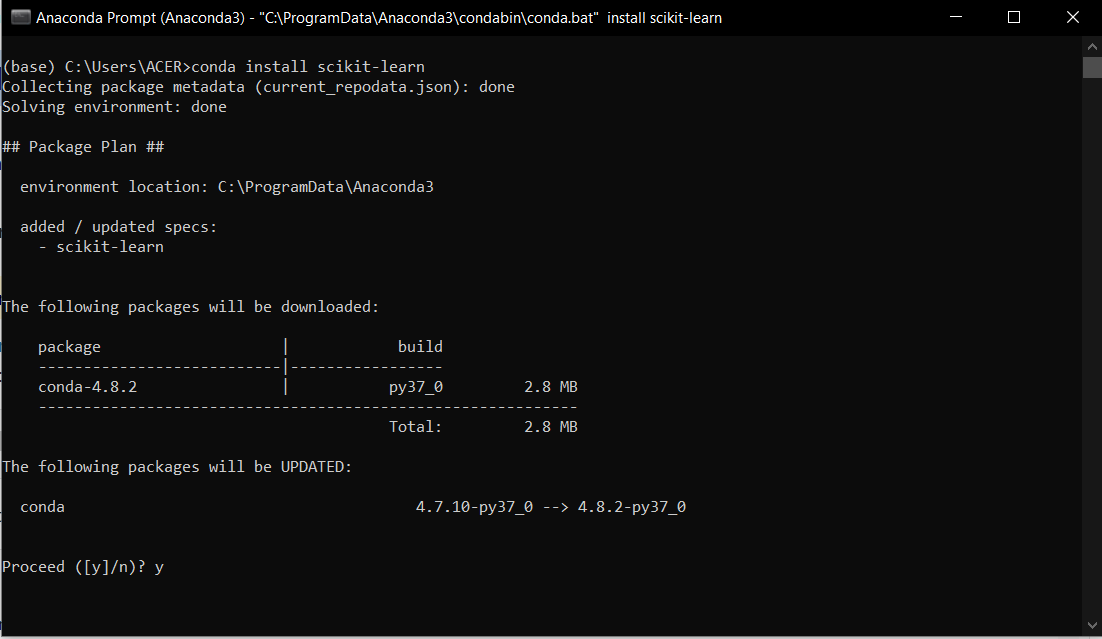
\includegraphics[width=4cm]{figures/1174070/1/1.PNG}
		\centering
		\caption{Instalasi Package Scikit Learn}
	\end{figure}
	\begin{figure}[H]
		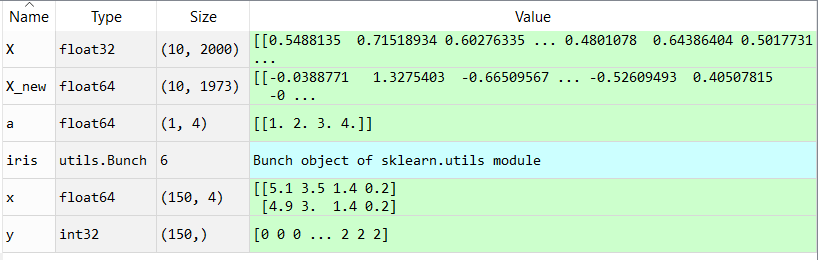
\includegraphics[width=4cm]{figures/1174070/1/2.PNG}
		\centering
		\caption{Isi Variabel Explorer}
	\end{figure}
	\item Mencoba loading an example dataset
	\hfill\break
	\lstinputlisting[firstline=8, lastline=12]{src/1174070/1/1174070.py}
	\item Mencoba Learning dan predicting
	\hfill\break
	\lstinputlisting[firstline=14, lastline=24]{src/1174070/1/1174070.py}
	\item Mencoba Model Persistence
	\hfill\break
	\lstinputlisting[firstline=26, lastline=36]{src/1174070/1/1174070.py}
	\item Mencoba Conventions
	\hfill\break
	\lstinputlisting[firstline=38, lastline=50]{src/1174070/1/1174070.py}
\end{enumerate}
\subsection{Penanganan Error}
\begin{enumerate}
	\item ScreenShoot Error
	\begin{figure}[H]
		\includegraphics[width=4cm]{figures/1174070/1/error/1.png}
		\centering
		\caption{Import Error}
	\end{figure}
	\begin{figure}[H]
		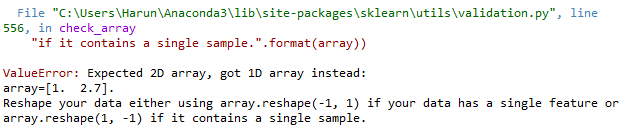
\includegraphics[width=4cm]{figures/1174070/1/error/2.png}
		\centering
		\caption{Value Error}
	\end{figure}
	\item Tuliskan Kode Error dan Jenis Error
	\begin{itemize}
		\item Import Error
		\item Value Error
	\end{itemize}
	\item Cara Penangan Error
	\begin{itemize}
		\item Import Error
		\hfill\break
		Dengan Menginstall Library Yang Tidak Ditemukan
		\item Value Error
		\hfill\break
		Mengubah Bentuk Arraynya, Menjadi 1 Dimensi
	\end{itemize}
\end{enumerate}
\subsection{Bukti Tidak Plagiat}
\begin{figure}[H]
	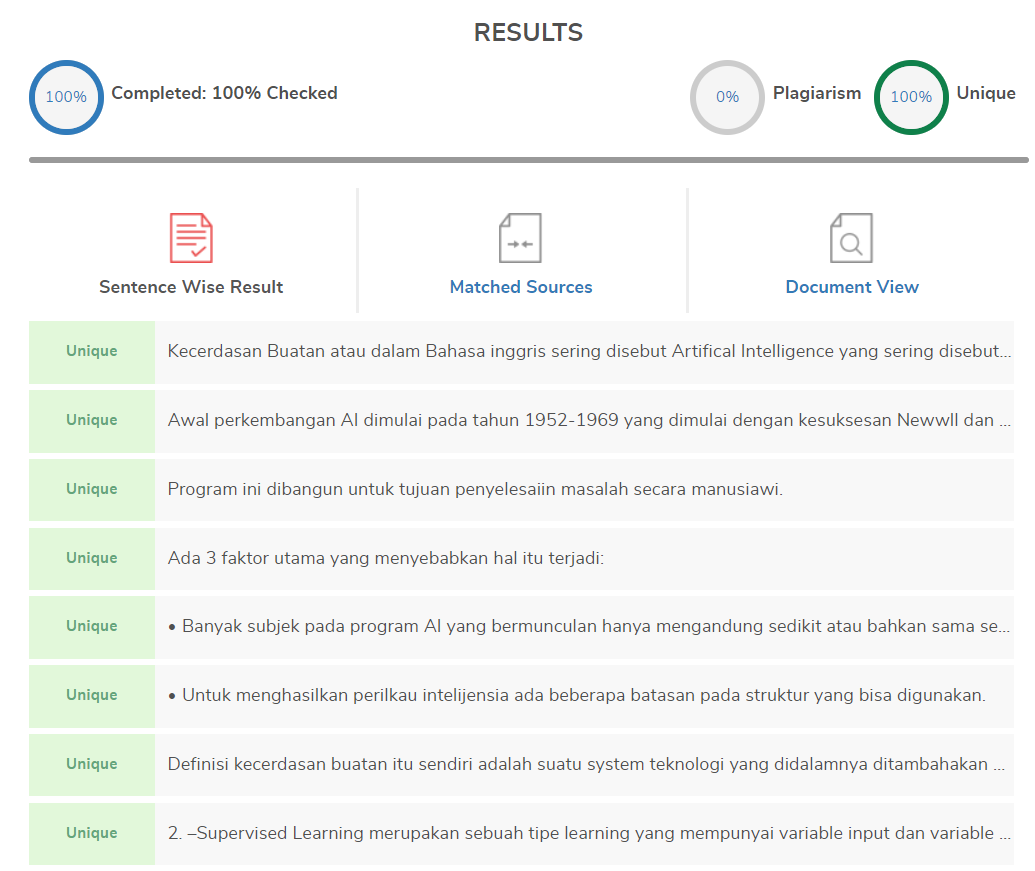
\includegraphics[width=4cm]{figures/1174070/1/plagiat/1.PNG}
	\centering
	\caption{Bukti Tidak Melakukan Plagiat 1}
    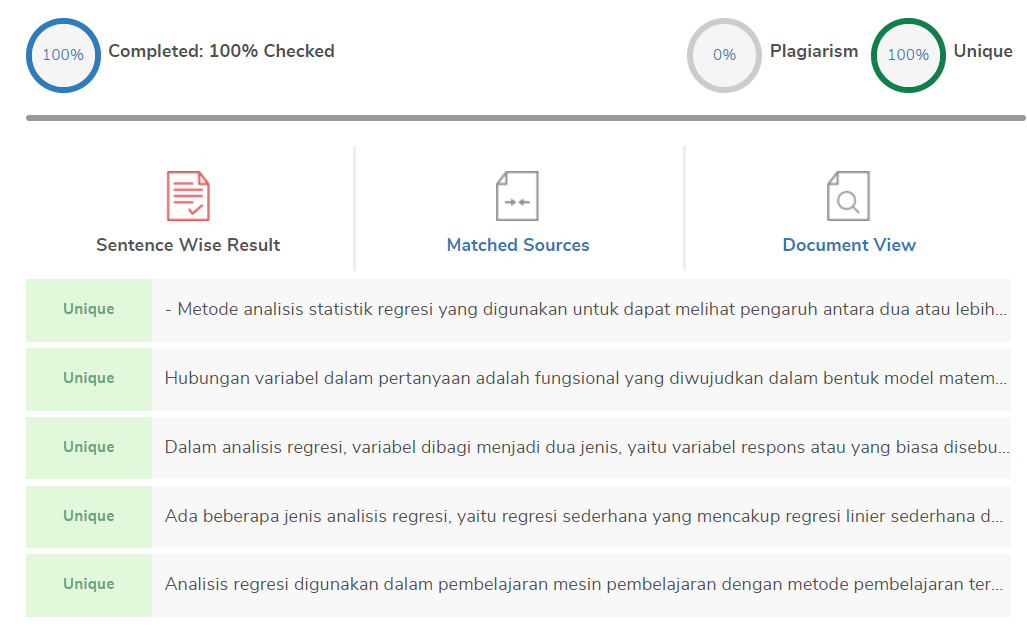
\includegraphics[width=4cm]{figures/1174070/1/plagiat/2.PNG}
	\centering
	\caption{Bukti Tidak Melakukan Plagiat 2}
\end{figure}
%\section{Fanny Shafira Damayanti (1174069)}
\subsection{Teori}
\begin{enumerate}
\item Definisi Kecerdasan buatan\\ 
Kecerdasan buatan atau Artificial intelligence merupakan kecerdasan yang ditambahkkan kedalam suatu system yang diatur secara ilmiah. Kecerdasan buatan dibuat untuk menggantikan pekerjaan yang dilakukan oleh manusia menjadi dikerjakan oleh sistem.

\item Sejarah Kecerdasan Buatan
\begin{itemize}
\item Abad 17, Rene Descartes berkata bahwa tubuh hewan adalah sekumpulan mesin yang rumit.
\item 1642, Blaise Pascal menciptakan mesin penghitung digital mekanis pertama.
\item Abad 19, Charles Babbage dan Ada Lovelace bekerja di program penghitung mekanis.
\item 1950, John McCarthy membuat istilah “Kecerdasan Buatan”.
\item 1960-1970, Joel Moses membuat program yang pertama kali sukses dalam bidang matematika.
\item 1980, jaringan saraf digunakan secara meluas dengan algoritme perambatan balik.
\item 2004, DARPA membuat kendaraan yang bisa dijalankan sendiri tanpa manusia.
\end{itemize}

\item Perkembangan kecerdasan buatan
\begin{itemize}
\item Masa persiapan (1943-1946)
Warren McCulloch dan Walter Pitt mengemukakan tiga hal : pengetahuan fisiologi dasar dan fungsi sel syaraf dalam otak, analisa formal tentang logika proposisi, dan teori komputasi Turing.

Pada tahun 1950, Nobert Wiener membuat penelitian mengenai prinsip-prinsip teori feedback.

Pada tahun 1956, John McCarthy meyakinkan Minsky, Claude Shannon dan Nathaniel Rochester untuk membantunya melakukan penelitian dalam bidan Otomata, Jaringan Syaraf dan pembelajaran intelijensia. 

\item Awal perkembangan (1952-1969)
Pada tahun 1958, McCarthy di MIT AI Lab Memo No.1 mendefinisikan bahasa pemrograman tingkat tinggi yaitu LISP,

Pada tahun 1959, Nathaniel Rochester dari IBM dan mahasiswa-mahasiswanya mengeluarkan program kecerdasan buatan yaitu Geometry Theorm Prover.

Pada tahun 1963, program yang dibuat James Slagle mampu menyelesaikan masalah integral tertutup untuk mata kuliah Kalkulus.
Pada tahun 1986, program analogi buatan Tom Evan menyelesaikan masalah analogi geometris yang ada pada tes IQ.

\item Perkembangan Kecerdasan Buatan Melambat (1969-1979)
Bruce Buchanan dan Joshua Lederberg yang membuat program untuk memecahkan masalah struktur molekul dari informasi yang didapatkan dari spectrometer massa.

\item AI Menjadi sebuah industri
Industrialisasi kecerdasan buatan diawali dengan ditemukannya sistem pakar yang dinamakan R1 yang mampu mengkonfigurasi system-sistem computer baru. 

\item Kembalinya Jaringan Syaraf Tiruan (1986-sekarang)
Pada tahun 1985-an setidaknya empat kelompok riset menemukan kembali algoritma belajar propagasi balik (Black-Propagation Learning). Algoritma ini berhasil diimplementasikan ke dalam bidang ilmu computer dan psikologi.
\end{itemize}

\item Definisi Supervised Learning\\
Supervised Learning merupakan cabang dari Artificial Intelligence. supervised learning adalah suatu ilmu yang mempelajari perancangan dan pengembangan algoritma.

\item Klasifikasi Supervised Learning
\begin{itemize}
\item Logistic regression.
\item K-nearest neighbors.
\item Support vector machine (SVM)
\item Naive Bayes.
\item Decision tree classification.
\item Random forest classification.
\end{itemize}

\item Regresi dan Unsupervised Learning\\
Regresi merupakan sebuah metode analisis statistic yang digunkan untuk mengetahui pengaruh antara dua variable atau lebih.

Untuk mempelajari Unsupervised learning kita tidak perlu data training untuk melakukan prediksi maupun klasifikasi.

\item Dataset\\
Dataset merupakan objek yang mempresentasikan data dan relasinya pada memori.

\item Training Set\\
Training Set merupakan bagian dari dataset untuk membuat prediksi atau menjalankan fungsi dari sebuah algoritma Machine Learning.

\item Testing Set\\
Testing set digunakan untuk mengukur apakah classifier berhasil melakukan klasifikasi dengan benar.

\end{enumerate}

\subsection{Instalasi}
\begin{enumerate}
	\item Instalasi Library scikit dari anaconda, mencoba kompilasi dan uji coba ambil contoh kode dan lihat variabel explorer
	\hfill\break
	\begin{figure}[H]
		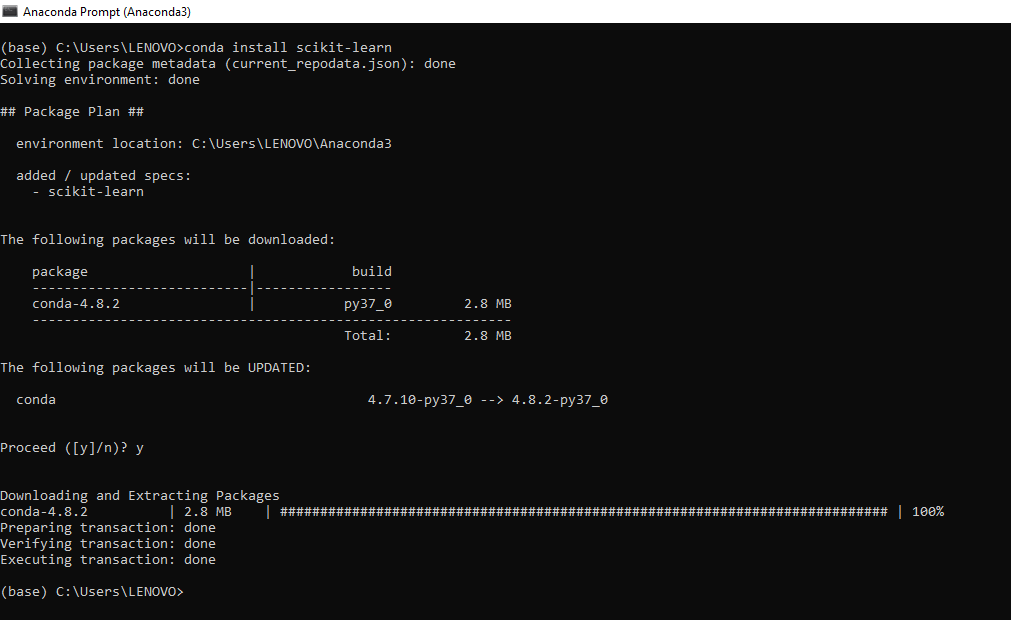
\includegraphics[width=4cm]{figures/1174069/1/1.png}
		\centering
		\caption{Instalasi Package Scikit Learn}
	\end{figure}
	\begin{figure}[H]
		\includegraphics[width=4cm]{figures/1174069/1/2.png}
		\centering
		\caption{Isi Variabel Explorer}
	\end{figure}
	\item Mencoba Loading an example dataset, menjelaskan maksud dari tulisan tersebut dan mengartikan           		  per baris
	\hfill\break
	\lstinputlisting[firstline=7, lastline=11]{src/1174069/1/1174069.py}
	\item Mencoba Learning and predicting, menjelaskan maksud dari tulisan tersebut dan mengartikan per  			  baris
	\hfill\break
	\lstinputlisting[firstline=13, lastline=22]{src/1174069/1/1174069.py}
	\item  Mencoba Model persistence, menjelaskan maksud dari tulisan tersebut dan mengartikan per baris
	\hfill\break
	\lstinputlisting[firstline=25, lastline=34]{src/1174069/1/1174069.py}
	\item Mencoba Conventions, menjelaskan maksud dari tulisan tersebut dan mengartikan per baris
	\hfill\break
	\lstinputlisting[firstline=37, lastline=48]{src/1174069/1/1174069.py}
\end{enumerate}

\subsection{Penanganan Error}
\begin{enumerate}
	\item ScreenShoot Error
	\begin{figure}[H]
		\includegraphics[width=4cm]{figures/1174069/1/error/1.png}
		\centering
		\caption{Import Error}
	\end{figure}

	\item Tuliskan Kode Error dan Jenis Error
	\begin{itemize}
		\item Import Error
	\end{itemize}
	\item Cara Penangan Error
	\begin{itemize}
		\item Import Error
		\hfill\break
		Dengan Menginstall Library Yang Tidak Ditemukan
	\end{itemize}
\end{enumerate}

\subsection{Bukti Tidak Plagiat}
\begin{figure}[H]
	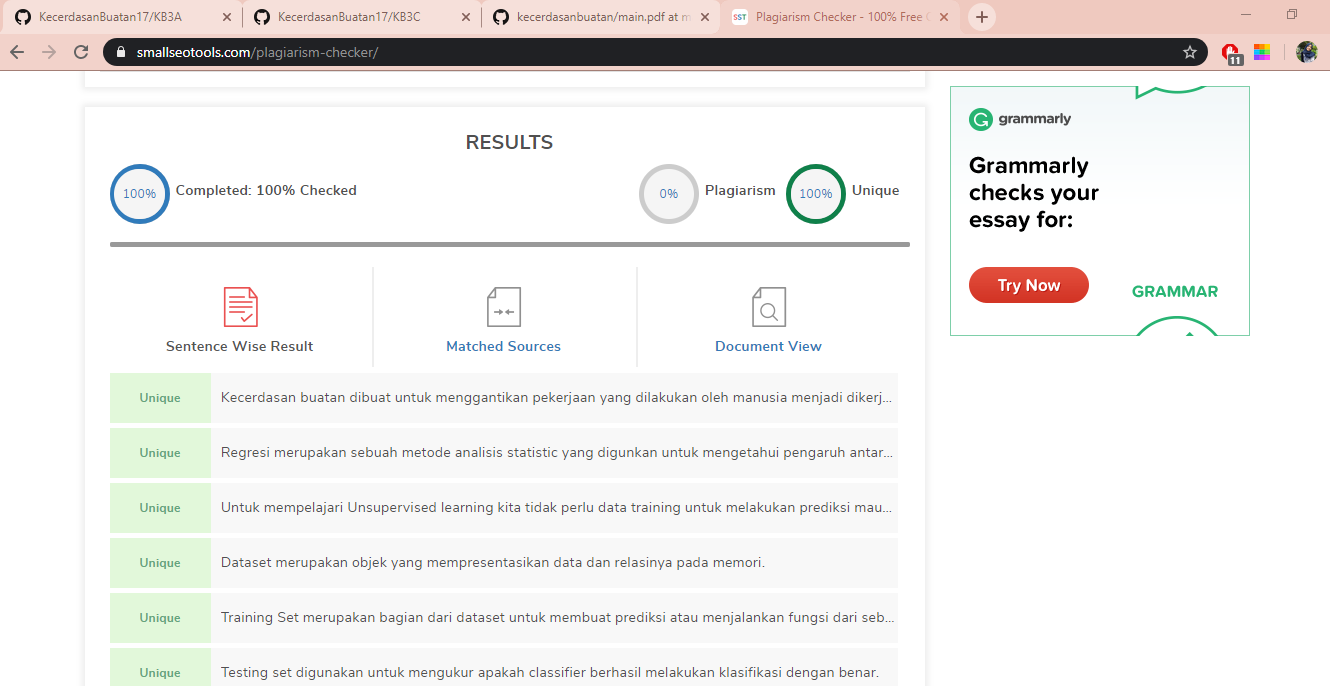
\includegraphics[width=4cm]{figures/1174069/1/plagiat/plagiat.png}
	\centering
	\caption{Bukti Tidak Melakukan Plagiat Chapter 1}
\end{figure}

\subsection{Link Youtube}


%\section{1174086 - Tia Nur Candida}
\subsection{Teori}
\begin{enumerate}
\item Definisi Kecerdasan Buatan\\
Kecerdasan Buatan adalah suatu ilmu yang mempelajari bagaimana cara komputer melakukan sesuatu seperti yang dilakukan oleh manusia. Secara sederhana AI adalah teknik dan ilmu untuk membangun atau membuat suatu mesin menjadi cerdas, terutama pada program komputer. Kecerdasan yang dimaksud yaitu seperti yang dimiliki oleh manusia namun pada mesin akan dibuat cepat dan tepat atau akurat.

\item Sejarah Kecerdasan Buatan
Sejarah kecerdasan buatan dimulai pada zaman kuno. Benih kecerdasan buatan modern ditanamkan oleh filusuf klasik dengan berusaha menggambarkan proses berpikir manusia. Karya tersebut memuncak pada penemuan komputer digital yang di program pada tahun 1940 an, dimana terdapat sebuah mesin yang didasarkan pada esensi abstrak penalaran matematika. 
Istilah kecerdasan buatan pertama kali dikemukaan pada tahun 1956 di Konferensi Darthmouth yang kemudian sejak saat itu kecerdasan buatan terus berkembang.

\item Perkembangan kecerdasan buatan
\begin{itemize}
\item Masa Persiapan AI (1943-1956)
Pada tahun 1943, Warren McCulloch dan Walter Pitt mengemukakan tiga hal : pengetahuan fisiologi dasar dan fungsi sel syaraf dalam otak, analisa formal tentang logika proposisi, dan teori komputasi Turing. Mereka berhasil membuat suatu model sel syaraf tiruan dimana setiap sel syaraf digambarkan sebagai ‘on’ dan ‘off’. Mereka menunjukkan bahwa setiap fungsi dapat dihitung dengan suatu jaringan sel syaraf dan bahwa semua hubungan logis dapat diimplementasikan dengan struktur jaringan yang sederhana.
Pada tahun 1950, Nobert Wiener membuat penelitian mengenai prinsip-prinsip teori feedback. Contoh yang terkenal adalah thermostat. Penemuan ini juga merupakan awal dari perkembangan AI.
Pada tahun 1956, John McCarthy meyakinkan Minsky, Claude Shannon dan Nathaniel Rochester untuk membantunya melakukan penelitian dalam bidan Otomata, Jaringan Syaraf dan pembelajaran intelijensia. Mereka mengerjakan proyek ini selama 2 bulan di Dartsmouth. Hasilnya adalah program yang mampu berpikir non-numerik dan menyelesaikan masalah pemikiran, yang dinamakan Principia Mathematica. Hal ini menjadikan McCarthy disebut sebagai bapak kecerdasan buatan.

\item Awal perkembangan AI (1952-1969)
Kecerdasan buatan banyak mengalami kesuksesan pada tahun pertama. 
Pada tahun 1958, McCarthy di MIT AI Lab Memo No.1 mendefinisikan bahasa pemrograman tingkat tinggi yaiyu LISP, yang sekarang mendominasi pembuatan program-pogram kecerdasan buatan. Kemudian, McCarthy membuat program yang dinamakan Programs with Common Sense. Di dalam program tersebut, dibuat rancangan untuk menggunakan pengetahuan dalam mencari solusi.
Pada tahun 1959, Nathaniel Rochester dari IBM dan mahasiswa-mahasiswanya mengeluarkan program kecerdasan buatan yaitu Geometry Theorm Prover. Program ini dapat mengeluarkan suatu teorema menggunakan aksioma-aksioma yang ada.
Pada tahun 1963, program yang dibuat James Slagle mampu menyelesaikan masalah integral tertutup untuk mata kuliah Kalkulus.
Pada tahun 1986, program analogi buatan Tom Evan menyelesaikan masalah analogi geometris yang ada pada tes IQ.

\item Perkembangan kecerdasan buatan melambat (1966-1974)
Banyak masalah yang perlu di selesaikan oleh kecerdasan buatan dan baru sedikit program yang keluar menyebabkan melambat.

\item Kecerdasan buatan menjadi sebuah industri ( 1980 - 1988 )
Industrialisasi kecerdasan buatan diawali dengan ditemukannya sistem pakar yang dinamakan R1 yang mampu mengkonfigurasi system-sistem computer baru. Program tersebut mulai dioperasikan di Digital Equipment Corporation (DEC), McDermott, pada tahun 1982.
Pada tahun 1986, R1 telah berhasil menghemat US Dolar 40 juta per tahun.
Pada tahun 1988, kelompok kecerdasan buatan di DEC menjalankan 40 sistem pakar. Hampir semua perusahaan besar di USA mempunyai divisi AI. Sehingga perusahaan yang sejak tahun 1982 hanya menghasilkan beberapa juta US dolar per tahun meningkat menjadi 2 milyar US dolar per tahun pada tahun 1988.

\item Kembalinya Jaringan Syaraf Tiruan ( 1986 - Sekarang )
Meskipun bidang ilmu computer menolak jaringan syaraf tiruan setelah diterbitkannya buku “Perceptrons” karangan Minsky dan Papert, tetapi para ilmuwan masih mempelajari bidang ilmu tersebut dari sudut pandang yang lain yaitu fisika. Para ahli fisika seperti Hopfield (1982) menggunakan teknik-teknik mekanika statistika untuk menganalisa sifat-sifat pentimpanan dan optimasi pada jaringan syaraf. Para ahli psikologi, David Rumelhart dan Geoff Hinton, melanjutkan penelitian mengenai model jaringan syaraf tiruan pada memori.
Pada tahun 1985-an setidaknya empat kelompok riset menemukan kembali algoritma belajar propagasi balik (Black-Propagation Learning). Algoritma ini berhasil diimplementasikan ke dalam bidang ilmu computer dan psikologi.

\end{itemize}
\item Definisi Supervised Learning\\

Merupakan tipe Machine Learning dimana model ini menyediakan training data berlabel. Supervised learning merupakan suatu pembelajaran yang terawasi dimana jika output yang diharapkan telah diketahui sebelumnya.  Supervised Learning adalah tipe learning di mana kita mempunyai variable input dan variable output, dan menggunakan satu algoritma atau lebih untuk mempelajari fungsi pemetaan dari input ke output. Goal-nya adalah untuk memperkirakan fungsi pemetaannya, sehingga ketika kita mempunya input baru, kita dapat memprediksi output untuk input tersebut.

\item Klasifikasi
\begin{itemize}
\item Logistic regression.
\item K-nearest neighbors.
\item Support vector machine (SVM).
\item Naive Bayes.
\item Decision tree classification.
\item Random forest classification.
\end{itemize}

\item Regresi \\
Regresi adalah suatu metode analisis statistik yang digunakan untuk melihat pengaruh antara dua atau lebih banyak variabel. Hubungan variabel tersebut bersifat fungsional yang diwujudkan dalam suatu model matematis.

\item Unsupervised Learning \\
Unsupervised Learning adalah tipe learning di mana kita hanya mempunyai data masukan (input data) tetapi tidak ada output variable yang berhubungan.\\
Goal dari unsupervised learning adalah untuk memodelkan struktur dasar atau distribusi dalam data dengan tujuan untuk mempelajari data lebih jauh lagi, dengan kata lain, adalah menyimpulkan fungsi yang mendeskripsikan atau menjelaskan data.

\item Dataset \\
Dataset adalah objek yang merepresentasikan data dan relasinya di memory. Strukturnya mirip dengan data di database. Dataset berisi koleksi dari datatable dan datarelation.
\item Training Set \\
Training set adalah bagian dataset yang kita latih untuk membuat prediksi atau menjalankan fungsi dari sebuah algoritma ML lainnya sesuai tujuannya masing-masing. Kita memberikan petunjuk melalui algoritma agar mesin yang kita latih bisa mencari korelasinya sendiri.
\item Test Set \\
Test set adalah bagian dataset yang kita tes untuk melihat keakuratannya, atau dengan kata lain melihat performanya.

\end{enumerate}

\subsection{Praktek}
\begin{enumerate}
	\item Instalasi Library scikit dari anaconda, mencoba kompilasi dan uji coba ambil contoh kode dan lihat variabel explorer
	\hfill\break
	\begin{figure}[H]
		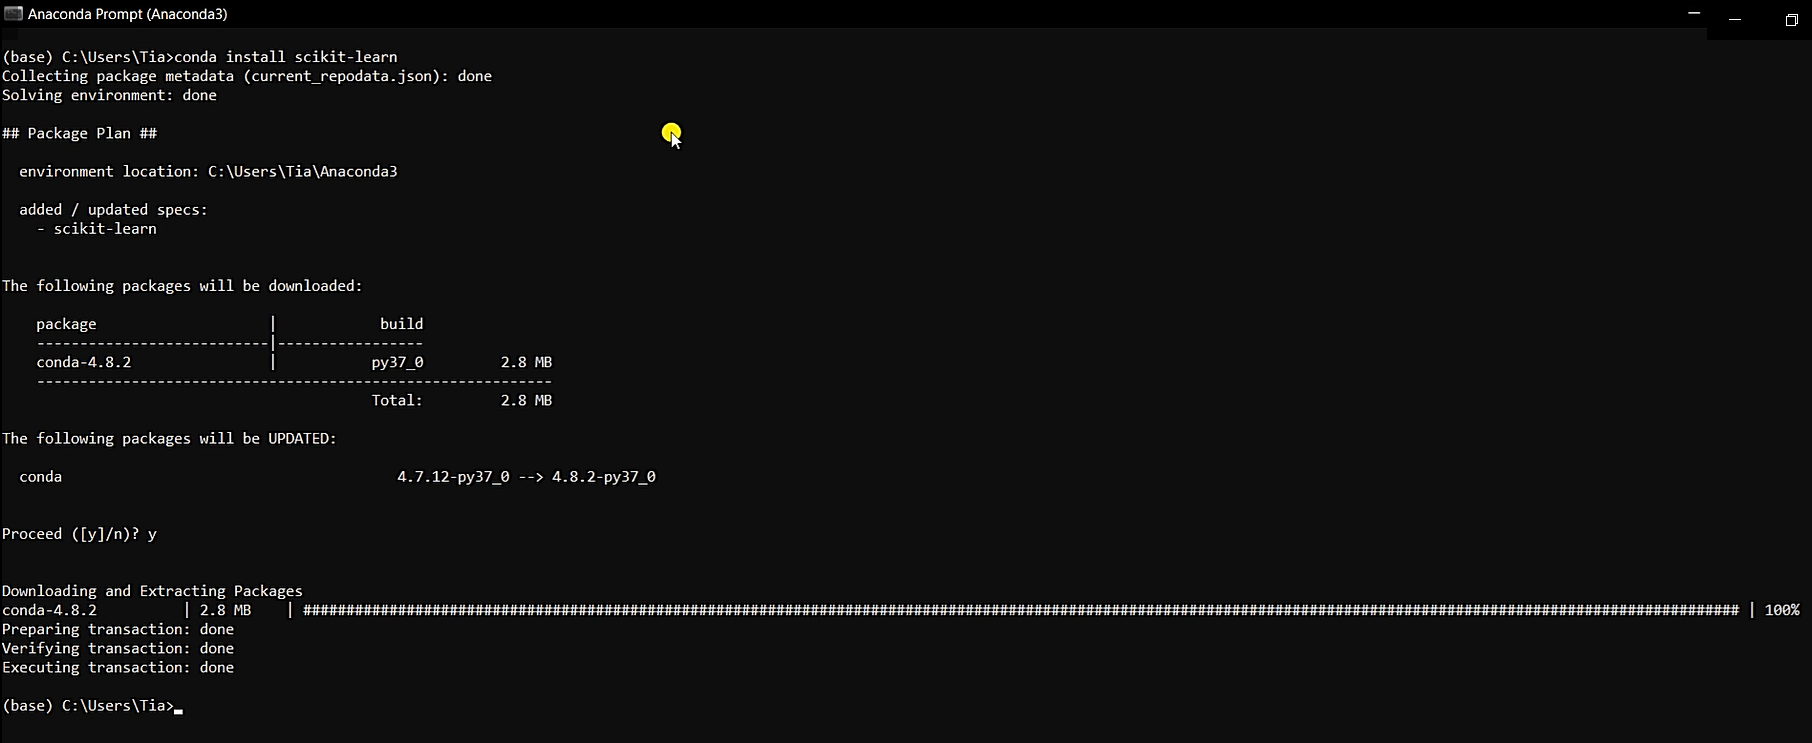
\includegraphics[width=4cm]{figures/1174086/1/installasi.png}
		\centering
		\caption{Instalasi Package Scikit Learn}
	\end{figure}
	\begin{figure}[H]
		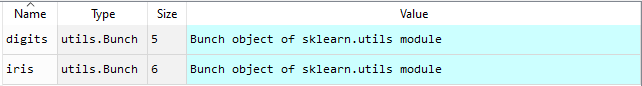
\includegraphics[width=4cm]{figures/1174086/1/variabel.png}
		\centering
		\caption{Isi Variabel Explorer}
	\end{figure}
	\item Mencoba loading an example dataset
	\hfill\break
	\lstinputlisting[firstline=7, lastline=11]{src/1174086/1/1174086.py}
	\item Mencoba Learning dan predicting
	\hfill\break
	\lstinputlisting[firstline=13, lastline=22]{src/1174086/1/1174086.py}
	\item Mencoba Model Persistence
	\hfill\break
	\lstinputlisting[firstline=25, lastline=34]{src/1174086/1/1174086.py}
	\item Mencoba Conventions
	\hfill\break
	\lstinputlisting[firstline=37, lastline=48]{src/1174086/1/1174086.py}
\end{enumerate}

\subsection{Penanganan Error}
\begin{enumerate}
	\item ScreenShoot Error
	\begin{figure}[H]
		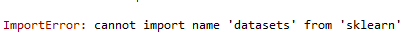
\includegraphics[width=4cm]{figures/1174086/error/1_import.png}
		\centering
		\caption{Import Error}
	\end{figure}
	\begin{figure}[H]
		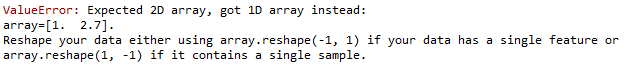
\includegraphics[width=4cm]{figures/1174086/error/1_value.png}
		\centering
		\caption{Value Error}
	\end{figure}
	\item Tuliskan Kode Error dan Jenis Error
	\begin{itemize}
		\item Import Error
		\item Value Error
	\end{itemize}
	\item Cara Penangan Error
	\begin{itemize}
		\item Import Error
		\hfill\break
		Dengan Menginstall Library Yang Tidak Ditemukan
		\item Value Error
		\hfill\break
		Mengubah Bentuk Arraynya, Menjadi 1 Dimensi
	\end{itemize}
\end{enumerate}

\subsection{Bukti Tidak Plagiat}
\begin{figure}[H]
	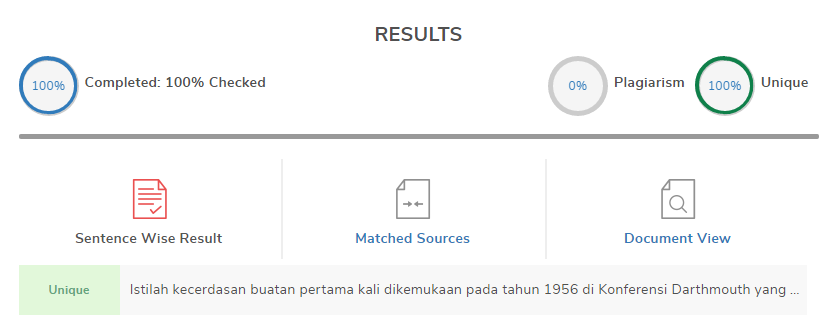
\includegraphics[width=4cm]{figures/1174086/bukti/1.png}
	\centering
	\caption{Bukti Tidak Melakukan Plagiat Chapter 1}
\end{figure}



%\section{1174054 | Aulyardha Anindita}

\subsection{Teori}
\begin{enumerate}
\item Definisi, Sejarah dan Perkembangan Kecerdasan Buatan
\begin{itemize}
\item Definisi Kecerdasan Buatan\\
Kecerdasan buatan adalah suatu kecerdasan yang didalamnya berisi suatu system yang biasa diatur dalam sebuah konteks ilmiah. Kecerdasan  buatan juga bisa didefinisikan sebagai sebuah kecerdasan yang diciptakan dan dimasukkan kedalam suatu mesin computer agar dapat melakukan pekerjaan seperti yang dapat dilakukan oleh manusia. Ada beberapa macam bidang atau ilmu yang menggunakan kecerdasan buatan diantaranya adalah system pakar, permainan computer (game), logika fuzzy, jaringan saraf tiruan dan robotika.\\
Penelitian dalam AI mencakup pembuatan mesin dan suatu program computer untuk mengotomatisasikan tugas-tugas yang membutuhkan perilaku cerdas, seperti : pengendalian, perencanaan dan penjadwalan serta kemampuan untuk menjawab diagnose dan pertanyaan pelanggan serta pengenalan tulisan tangan. Suara dan wajah

\item Sejarah Kecerdasan Buatan
\begin{itemize}
\item Pada tahun 1940 dan 1950 Artificial Inteligence merupakan suatu inovasi baru dalam bidang ilmu pengetahuan dimana pada tahun ini computer modern sudah ada
\item Pada tahun 1950 awal, studi tentang “mesin berfikir” mempunyai berbegai nama seperti cybernetics, teori automata, dan pemrosesan informasi
\item Pada tahun 1956, para ilmuwan jenius seperti Alan Turing, Norbert, Wiener, Claude Shannon dan Warren McCullough bekerja secara independen di bidang cybernetics, matematika, algoritma dan teori jaringan. John McCarthy merupakan orang yang menciptakan istilah tersebut dan mendirikan laboratorium kecerdasan buatan di MIT dan Stanford
\item Pada tahun 1956, McCarthy mendirikan Konferensi Dartmouth di Hanover, New Hampshire. Dia merupakan peneliti terkemuka dalam teori kompleksitas, simulasi Bahasa, dan hubungan antara keacakan dan pemikiran kreatif, jaringan saraf diundang. Sehingga Konferensi Dartmouth 1956 dianggap sebagai kelahiran Kecerdasan Buatan.
\item Sejak saat itu, Kecerdasan Buatan telah hidup melalui decade kemuliaan dan cemohan yang dikenal dengan luas sebagai musim panas dan musim dingin Ai.
\end{itemize}

\item Perkembangan Kecerdasan Buatan\\
Saat ini, teknologi Artificial Intelligence sangat ramai diperbincangkan oleh masyarakat. Sudah banyak pekerjaan yang hilang karena adanya AI, seperti pekerjaan kasir, penjaga pintu tol, parkir, dan sebagainya. Hal ini terjadi karena AI lebih unggul dalam hal kinerja, fitur dan lain sebagainya. Walaupun masih ada beberapa aspek yang memang pekerja manusia masih unggul dibandingkan AI itu sendiri. \\
Berdasarkan survei yang dilakukan oleh Microsoft, hasilnya adalah 39 responden masih mempertimbangkan untuk menggunakan mobil tanpa pengemudi dan sebanyak 36 responden lainnya setuju mahwa robot atau AI dengan menggunakan software untuk beroperasi mampu meningkatan produktivitas. Dari survei tersebut, dapat ditarik kesimpulan bahwa pengguna AI harus lebih bijaksana dalam pengembangan dan penggunaan dari AI sehingga tidak memiliki efek samping terhadap profuktifitas kerja dan keseharian sebagai pengguna dalam kehidupan sehari-hari.

\end{itemize}

\item Definisi Supervised Learning, Klasifikasi, Regresi, Unsupervised Learning, Data Set, Training Set dan Testing Set
\begin{itemize}
\item Supervised Learning\\
Supervised learning adalah suatu tugas pengumpulan data yang berfungsi untum menyimpulkan fungsi dari data pelatihan yang berlabel. Didalam Supervised Learning, setiap contoh merupakan pasangan yang terdiri dari objek input dan nilai output yang diinginkan. Algoritma pembelajaran yang diawasi berupa menganalisis data pelatihan dan menghasilkan fungsi yang disimpulkan yang digunakan untuk memetakan contoh baru.\\
 	Supervised Learning adalah suatu pendekatan dimana sudah terdapat data yang dilatih selain itu juga sudah memiliki variable yang ditargetkan sehingga tujuan dari pendekatan tersebut adalah mengelompokkan suatu data ke data yang sudah ada. Supervised learning sendiri menyediakan algoritma pembelajaran dengan jumlah yang diketahui untuk mendukung penilaian dimasa depan. Supervised learning sebagian besar memiliki kaitan dengan AI dengan menggunakan model pembelajaran generatif. Data pelatihan untuk pembelajaran yang diawasi mencakup beberapa contoh dengan subjek input yang berpasangan dan output yang diinginkan.\\
 	Modul supervised learning mempunyai beberapa keunggulan dibandingkan pendekatan tanpa pengawasan, tapi mereka juga memiliki keterbatasan. System lebih cenderung membuat penilaian bahwa manusia dapat berhubungan, misalnya manusia mempunyai dasar untuk keputusan. Tapi, dalam kasus tersebut yang menggunakan metode berbasis pengambilan, supervised learning mengalami kseulitan dalam menangani suatu informasi baru. 

\item Klasifikasi\\
Klasifikasi merupakan pembagian menurut kelas-kelas. Menurut ilmu pengetahuan, klasifikasi adalah suatu proses pengelompokkan benda berdasarkan ciri-ciri persamaan dan perbedaan. Dalam pembelajaran mesin dan statistic, klasifikasi merupakan suatu pendekatan pembelajaran yang diawasi dimana program computer tersebut belajar dari input data yang diberkan kepadanya lalu menggunakan pembelajaran tersebut untuk mengklasifikasikan pengamatan baru. Kumpulan data tersebut mungkin hanya bersifat dua kelas atau mungkin juga multi-kelas.

\item Regresi\\
Regresi adalah suatu metode analisis statistik yang digunakan untuk melihat pengaruh antara dua atau lebih variable. Regresi sendiri membahas masalah ketika variable output yaitu nilai ril atau berkelanjutan seperti gaji atau berat. Banyak model yang dapat digunakan, yang paling sederhana adalah regresi linear.

\item Unsupervised Learning\\
Unsupervised learning berbeda dengan supervised learning, perbedaanya yaitu unsupervised learning tidak memiliki data pelatihan, sehingga data dapat dikelompokkan menjadi dua atau 3 begitupun seterusnya. Unsupervised learning adalah suatu pelatihan algoritma kecerdasan buatan (AI) menggunakan beberapa informasi yang tidak diklasifikasikan atau diberi label dan memungkinkan algoritma  untuk bertindak atas informasi tersebut. System AI disini dapat dikelompokkan berdasarkan informasi yang tidak disortir berdasarkan persamaan dan perbedaan meskipun tidak ada kategori yang disediakan. System AI disajikan dengan data yang tidak berlabel, tidak terkategorisasi dan algoritma system bekerja pada data tanpa pelatihan sebelumnya sehingga outputmya tergantung pada algoritma kode.

\item Data Set\\
Data set adalah suatu objek yang merepresentasikan data dan memiliki relasi yang ada di dalam memory. Struktur data set mirip dengan data yang ada didatabase, namun bedanya data set berisi koleksi dari data table dan data relation. Untuk mendapatkan data yang tepat, berarti mengumpulkan atau mengidentifikasi data yang berkorelasi dengan hasil yang ingin anda prediksi.

\item Training Set\\
Training set adalah salah satu set yang biasa digunakan oleh algoritma klasifikasi. Seperti decision tree, bayesian, neural network, dll. Mereka dapat digunakan untuk membentuk model classifier, dalam menjalankan pelatihan yang diatur melalui jaringan saraf yang mengajarkan pada net dengan cara menimbang berbagai fitur, menyesuaikan koefisien berdasarkan kemungkinan mereka meminimalkan kesalahan. Kofiesen tersebut juga dikenal sebagai parameter.

\item Testing Set\\
Testing set adalah salah satu set yang digunakan untuk mengukur sejauh mana classifier berhasil melakukan klasifikasi dengan benar. Hal ini berfungsi sebagai materai persetujuan tapi tak digunakan sampai akhir. Setelah melatih dan mengoptimalkan data, kita dapat melakukan pengujian sarat terhadap pengambilan sampel aca. Dan hasilnya harus memvalidasi bahwa jaring data tersebut secara akurat mengenali gambar atau mengenali setidaknya (x) dari jumlah tersebut.

\end{itemize}
\end{enumerate}

\subsection{Praktek}
\begin{enumerate}
\item Instalasi library scikit dari anaconda
\hfill\break
	\begin{figure}[H]
		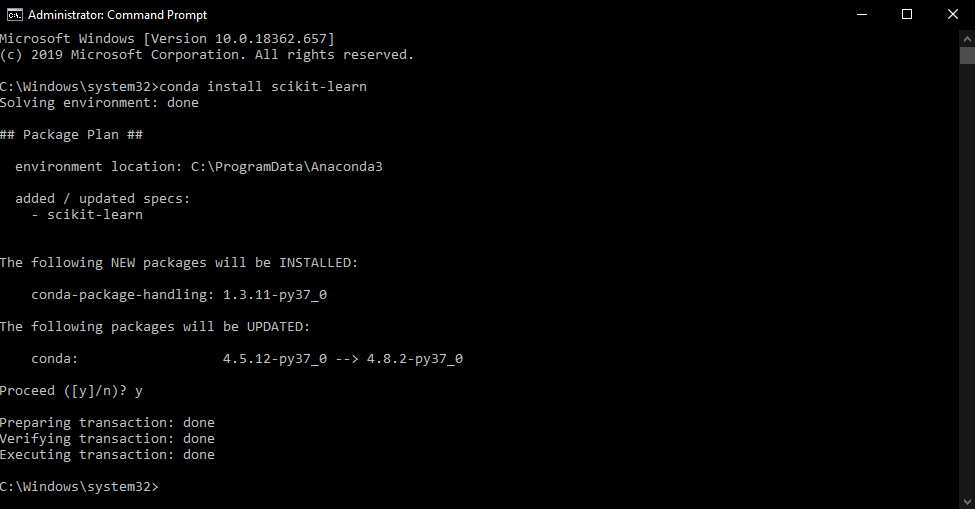
\includegraphics[width=4cm]{figures/1174054/1/1.png}
		\centering
		\caption{Instalasi Package Scikit Learn}
	\end{figure}
	\begin{figure}[H]
		\includegraphics[width=4cm]{figures/1174054/1/2.png}
		\centering
		\caption{Isi Variabel Explorer}
	\end{figure}
\item Mencoba Loading an example dataset
\hfill\break
	\lstinputlisting[firstline=8, lastline=12]{src/1174054/1/1174054.py}
	
\item Mencoba Learning and predicting
\hfill\break
	\lstinputlisting[firstline=14, lastline=24]{src/1174054/1/1174054.py}
	
\item Mencoba Model persistence
\hfill\break
	\lstinputlisting[firstline=26, lastline=36]{src/1174054/1/1174054.py}
	
\item Mencoba Conventions
\hfill\break
	\lstinputlisting[firstline=38, lastline=50]{src/1174054/1/1174054.py}
\end{enumerate}

\subsection{Penanganan Error}
\begin{enumerate}
\item ScreenShoot Error
	\begin{figure}[H]
		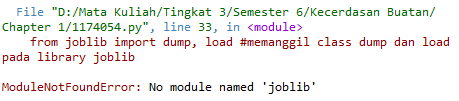
\includegraphics[width=4cm]{figures/1174054/1/3.png}
		\centering
		\caption{Module Not Found Error}
	\end{figure}
	\begin{figure}[H]
		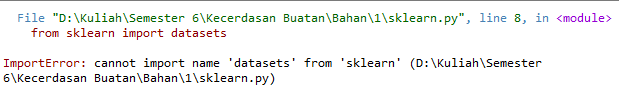
\includegraphics[width=4cm]{figures/1174054/1/4.png}
		\centering
		\caption{Import Error}
	\end{figure}

	\item Tuliskan Kode Error dan Jenis Error
	\begin{itemize}
		\item Module Not Found Error
		\item Import Error
	\end{itemize}
	\item Cara Penanganan Error
	\begin{itemize}
		\item Module Not Found Error
		\hfill\break
		Dengan memperbaiki penulisan atau kesalahan dalam penulisan kode atau melakukan install package atau modul yang belum terinstal
		\item Import Error
		\hfill\break
		Dengan Menginstall Library Yang Tidak Ditemukan
	\end{itemize}
\end{enumerate}


\subsection{Bukti Tidak Plagiat}
\begin{figure}[H]
	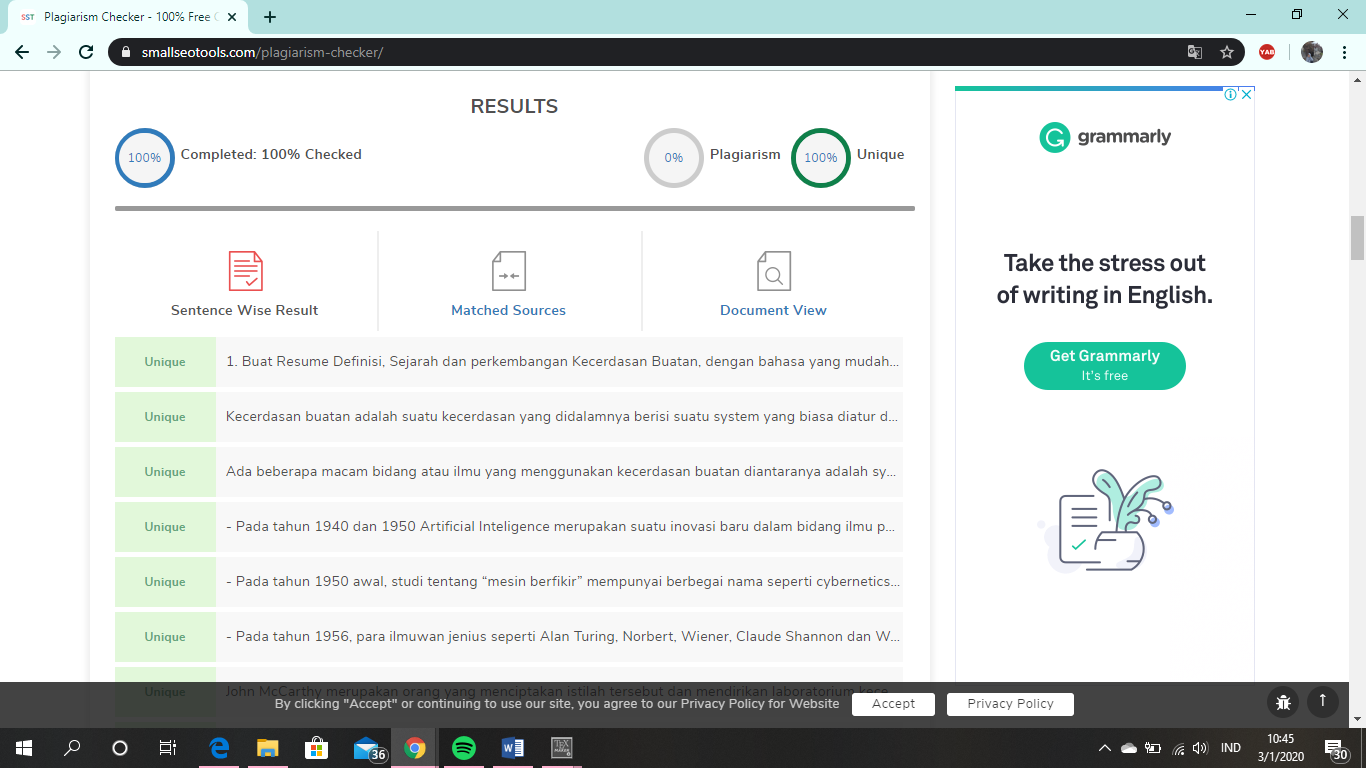
\includegraphics[width=4cm]{figures/1174054/1/plagiarisme.png}
	\centering
	\caption{Bukti Plagiasrisme}
\end{figure}

\subsection{Link Youtube}
https://youtu.be/gl9Q60DzEfI
%\section{Ainul Filiani 1174073}
\subsection{Pengertian Kecerdasan Buatan}
kecerdasan buatan adalah salah satu cabang ilmu pengetahuan yang berhubungan dengan mesin untuk memecahkan persoalan yang rumit dengan cara yang lebih manusiawi. Hal ini biasanya dilakukan dengan mengikuti karakteristik dan anologi berpikir dari kecerdasan  atau inteligance manusia, dan menerapkan sebagai algoritma yang dikenal oleh komputer.
Dengan suatu pendekatan yang kurang lebih fleksibilitas dan efisien dapat diambil tergantung keperluan yang mempengaruhi bagaimana wujud dari prilaku kecerdasan buatan. AI biasanya dihubungkan dengan ilmu komputer, akan tetapi juga terkait erat dengan bidang lain seperti matematika, Psikologi, Pengamatan, Biolog, filosofi, dan lainnya
\subsection{Sejarah Kecerdasan Buatan}
Kecerdasan buatan merupakan bidang ilmu komputer yang sangat penting di era kini dan masa yang akan datang untuk mewujudkan sistem komputer yang cerdas. Bidang ini telah berkembang sangat pesat di 20 tahun terakir seiring dengan kebutuhan perangkat cerdas pada industry dan rumah tangga.
Kata Intelligance berasal dari bahasa latin "intelligo" yang berarti "saya paham". Berarti dasar dari intelligance adalah kemampuan untuk memahami dan melakukan aksi. nyatanya, bidang Kecerdasan Buatan atau disingkat dengan AI, berawal dari kemunculan komputer sekitar tahun 1940-an, sedangkan perkembangan sejarah dapat ditelusuri sejak zaman Mesir kuno. Pada saat ini, perhatian mendesak diberikan pada kemampuan komputer untuk melakukan hal-hal yang dapat dilakukan manusia. Dalam hal ini, komputer ini dapat meningkatkan kemampuan kecerdasan dan kecerdasan manusia.
Pada awal abad ke-17, René berbicara tentang tubuh binatang yang tidak meminta apa pun selain mesin yang rumit. Blaise Pascal membuat mesin hitung digital mekanis pertama pada tahun 1642. Pada 19, Charles Babbage dan Ada Lovelace bekerja pada mesin hitung mekanis yang dapat diprogram. Bertrand Russell dan Alfred Whitehead North menerbitkan Principia Mathematica, yang merombak logistik formal. Warren McCulloch dan Walter Pitts menerbitkan "Kalkulus Logika Gagasan yang Menjaga Aktivitas" pada tahun 1943 yang membentuk dasar bagi jaringan saraf.
1950-an adalah periode upaya aktif dalam AI. program permainan catur yang ditulis oleh Dietrich Prinz. John McCarthy menciptakan istilah "kecerdasan buatan" pada konferensi pertama yang menjadi dasar perjanjian itu, pada tahun 1956. Dia juga menemukan bahasa pemrograman Lisp. Alan Turing memperkenalkan "tes Turing" sebagai cara untuk mengoperasionalkan tes kecerdasan cerdas. 
\subsection{Perkembangan dan Penggunaan Kecerdasan}
Menurut studi Harvard Business Review dan ICM Unlimited pada tahun 2016, perusahaan besar memberikan kompensasi 10 persen lebih tinggi untuk setiap karyawan, Terrelong melanjutkan pengembangan Artificial Intelligence (AI) tidak hanya untuk membuat gambar atau video palsu lebih mudah, tetapi juga membuatnya sulit untuk membuktikan materi.Meskipun pada saat ini, upaya untuk membuat dan mendistribusikan konten hoax, alias hoaks, masih dapat diatasi, tetapi berhasil, tantangan yang dihadapi semakin sulit. Selain itu, AI memungkinkan pembuatan gambar, video, atau audio palsu dari bahan yang relatif minim.Moody's, yang harus disetujui, membuktikan upaya itu akan semakin menantang dan membutuhkan teknik forensik yang lebih canggih.Pada Mei 2019, para peneliti di Samsung AI Center dan Institut Sains dan Teknologi Skolkovo di Moskow, Rusia menunjukkan bahwa mereka dapat membuat tayangan video yang menampilkan masing-masing individu. Video ini sangat realistis tetapi sebenarnya palsu, dibuat menggunakan model pembelajaran tertentu yang disebut Generative Adversarial Network (GAN).Hasil dari proses GAN disebut deepfakes karena mereka menggunakan teknik pembelajaran yang mendalam untuk membuat konten palsu.Untuk jangka pendek, perusahaan diharapkan untuk terus memainkan media sosial dan situs untuk melihat pentingnya disinformasi dan meminta mereka yang bertanggung jawab untuk media sosial dan situs terkait untuk mengunduh konten.Terrelonge menambahkan langkah lain yang bisa diambil untuk merilis materi resmi untuk melawan konten palsu."Perlawanan terhadap konten palsu membutuhkan kombinasi teknologi dan pendidikan,".
\section{resume mengenai definisi supervised learning, klarifikasi, regresi, dan un-supervised learning. Data Set, training set dan testing set}
\subsection{Sipervised Learning}Supervised Learning adalah tugas mengumpulkan data untuk melengkapi fungsi data pelatihan yang diberi label. Data pelatihan terdiri dari contoh pelatihan. Dalam pembelajaran terawasi, setiap contoh adalah pasangan yang terdiri dari objek input (biasanya vektor) dan nilai output dingin (juga disebut sinyal pengawasan super). Algoritma pembelajaran yang diawasi menganalisis data pelatihan dan menghasilkan fungsi yang lengkap, yang dapat digunakan untuk memetakan contoh-contoh baru. Skenario  akan memungkinkan algoritma menentukan lable kelas dengan benar untuk instance yang tidak terlihat. Ini membutuhkan algoritma pembelajaran untuk menggeneralisasi data pelatihan sehingga tidak muncul dengan cara yang "masuk akal". Pembelajaran terawasi semakin dekat di mana ada pelatihan praktis selain dapat bervariasi yang berarti tujuannya adalah di mana mengelompokkan data ke dalam database yang ada. Pembelajaran terawasi menyediakan jumlah pembelajaran yang direkomendasikan untuk mendukung penilaian di masa depan. Obrolan, program mengemudi mandiri, pengenalan wajah, tatap muka dan robot adalah beberapa sistem yang dapat menggunakan pembelajaran yang diawasi atau tidak diawasi. Pembelajaran terbimbing sebagian besar terkait dengan AI berdasarkan pengambilan mereka juga mungkin diperlukan menggunakan model pembelajaran generatif. Pelatihan data untuk pembelajaran dimulai dengan mendiskusikan contoh-contoh dengan subjek input berpasangan dan output yang diinginkan (juga disebut sebagai sinyal pengawasan). Dalam pembelajaran yang diawasi untuk pemrosesan gambar, misalnya sistem AI dapat lengkap dengan gambar mengemudi yang berlabel dalam kategori mobil dan truk. Setelah jumlah yang memadai, sistem harus dapat membedakan antara dan mengklasifikasikan gambar yang tidak berlabel, di mana waktu pelatihan dapat diselesaikan secara penuh. Model Pembelajaran Terpandu memiliki beberapa keunggulan dibandingkan pengawasan, tetapi mereka juga memiliki keterbatasan. Sistem lebih cenderung membuat penilaian bahwa hak asasi manusia dapat dihubungkan, misalnya karena manusia telah memberikan dasar untuk pengambilan keputusan. Namun, dalam hal metode berbasis pengambilan, Supervised Learning menghilangkan kesulitan dalam menangani informasi baru. Jika sistem dikategorikan untuk mobil dan truk, maka sepeda disediakan, misalnya, harus dikelompokkan dalam satu kategori atau yang lain. Namun. Jika sistem AI generatif, mungkin tidak tahu apa itu sepeda tetapi akan dapat mengenalinya sebagai milik kategori yang terpisah.
\subsection{Klasifikasi}
Klasifikasi adalah pembagian hal sesuai dengan kelas (kelas). Menurut Science, klasifikasi adalah proses pengelompokan materi berdasarkan karakteristik dan perbedaan yang sama. Dalam masalah klasifikasi, kami mencoba memprediksi sejumlah nilai yang terpisah. Label (y) Umumnya datang dalam bentuk kategorikal dan mewakili sejumlah kelas. Dalam pembelajaran statistik dan pembelajaran mesin statistik, klasifikasi adalah pembelajaran yang dimulai ketika sebuah program komputer belajar dari input data yang disediakan untuk mendukung dan kemudian menggunakan pembelajaran ini untuk mengklasifikasikan pembelajaran baru. Pengumpulan data ini mungkin hanya dua kelas (seperti mengidentifikasi apakah orang ini laki-laki atau perempuan atau orang itu adalah spam atau bukan-spam) atau mungkin juga multi-kelas. Beberapa contoh masalah klasifikasi adalah: pengenalan ucapan, pengenalan tulisan tangan, metrik identifikasi, klasifikasi dokumen dll.
\subsection{Regresi}
Regresi adalah metode analisis statistik yang digunakan untuk melihat perbedaan antara dua atau lebih variabel. Regresi sedang membahas masalah kompilasi, variabel output adalah nilai nyata atau dipertahankan, seperti "gaji" atau "berat". Banyak model yang berbeda dapat digunakan untuk makan, cara paling sederhana adalah linearitas linear. Itu mencoba untuk mencocokkan data dengan pesawat-hyper terbaik yang melewati titik.
\subsection{unsupervised learning}
Belajar tanpa pengawasan berbeda dari Belajar dengan Supervisi. Perbedaannya adalah bahwa pembelajaran tanpa pengawasan tidak memiliki data pelatihan, jadi dari data yang tersedia kami mengelompokkan data menjadi 2 atau 3 bagian dan seterusnya. Unsupervised Learning adalah pelatihan dalam algoritma kecerdasan buatan (AI) menggunakan informasi yang tidak diklasifikasikan atau diberi label dan menyediakan algoritma untuk memperbaiki informasi yang diberikan tanpa bimbingan. Dalam Unattended Learning, sistem AI dapat mengklasifikasikan informasi yang tidak diurutkan berdasarkan ekuitas dan perbedaan dalam kategori mendadak yang disediakan. Dalam Supervised Learning Learning, sistem AI disajikan dengan sistem wajib yang tidak diberi label, tidak dikategorikan dan algoritma bekerja pada data tanpa pelatihan sebelumnya. Outputnya tergantung pada algoritma kode. Menyerahkan sistem untuk Belajar Tanpa Pengawasan adalah salah satu cara untuk menerima AI. Algoritma Pembelajaran tanpa pengawasan dapat melakukan tugas yang lebih kompleks daripada sistem pembelajaran yang diawasi. Namun, pembelajaran tanpa pengawasan dapat lebih tidak konsisten dengan model alternatif. Sementara Supervised Learning Might, misalnya, mencari sendiri dengan memilih kucing dari anjing, ia juga dapat menambahkan kategori yang tidak diinginkan dari yang tidak diinginkan untuk ditingkatkan menjadi ras yang tidak biasa, membuat pesanan diperlukan.
\subsection{Data Set}
Dataset adalah objek yang mewakili data dan hubungan dalam memori. Strukturnya mirip dengan basis data basis data, tetapi hanya kumpulan data yang dikumpulkan dari catatan dan latar belakang yang diaktifkan. dapatkan persetujuan yang tepat untuk mengumpulkan atau mengidentifikasi data yang berkorelasi dengan hasil yang ingin Anda hasilkan; yaitu data yang berisi sinyal tentang acara yang Anda sukai. Data harus disinkronkan dengan masalah yang Anda coba selesaikan. Gambar kucing bukan kompilasi yang sangat berguna. Anda sedang membangun sistem identifikasi wajah. Memodifikasi data yang selaras dengan masalah yang ingin Anda selesaikan harus dilakukan oleh para ahli data. Jika Anda tidak memiliki data yang benar, maka upaya Anda untuk membuat solusi AI harus kembali ke instalasi data. Format ujung kanan untuk belajar secara umum adalah array tensor, atau multi-dimensional. Jadi pipa data yang dibangun untuk pembelajaran dibangun secara umum untuk mengubah semua gambar, video, suara, suara, teks atau deret waktu menjadi vektor dan tensor yang dapat digunakan operasi aljabar linier. Data yang diperlukan perlu dinormalisasi, distandarisasi dan dikembalikan untuk meningkatkan kegunaannya, dan semua ini adalah langkah-langkah dalam pembelajaran mesin ETC. Deeplearning4j menawarkan alat ETV Data Vec untuk melakukan tugas memfasilitasi data.
Pembelajaran yang mendalam, dan pembelajaran mesin yang lebih umum, membutuhkan pelatihan yang baik agar dapat bekerja dengan baik. Mengumpulkan dan membangun satu set badan pelatihan yang cukup besar dari data yang diketahui membutuhkan waktu dan pengetahuan khusus tentang pengetahuan dan cara untuk mengumpulkan informasi yang relevan. Perangkat pelatihan bertindak sebagai patokan terhadap mana jaring pembelajaran dalam pengeboran. Itulah yang mereka perbarui untuk direkonstruksi sebelum mereka merilis data yang belum pernah dilihat sebelumnya. Pada saat ini, manusia memiliki pengetahuan luas tentang mengidentifikasi instrumen yang tepat dan mengubahnya menjadi representasi numerik yang dapat dipahami oleh algoritma pembelajaran dalam, tensor. Membangun set pelatihan, dalam arti tertentu, pra-pelatihan. Kumpulan pelatihan yang membutuhkan banyak waktu atau keahlian yang dapat membantu dalam dunia data dan pemecahan masalah. Sifat keahlian terbesar Anda dalam memberi tahu algoritma Anda apa yang penting bagi Anda adalah memilih apa yang Anda masukkan dalam kursus pelatihan Anda. Ini melibatkan menceritakan kisah melalui data awal yang Anda pilih untuk memandu proses pembelajaran mendalam Anda dengan mengekstraksi fitur-fitur penting, baik dalam pengaturan pelatihan dan data yang ingin Anda buat untuk dipelajari. Agar pelatihan ini bermanfaat, Anda harus memecahkan masalah yang Anda selesaikan; yaitu, apa yang Anda inginkan agar sesuai dengan pembelajaran Anda, di mana hasil yang ingin Anda prediksi.
\subsection{Training Set}
Set Pelatihan adalah set yang digunakan oleh algoritma klasifikasi. Dapat dicontohkan oleh: decisiontree, bayesian, neural network dll. Semuanya dapat digunakan untuk membuat model kelas. Terkait dengan pelatihan yang mengatur melalui jaringan saraf di internet bagaimana menimbang berbagai fitur, sesuaikan koefisien sesuai dengan apa yang mereka tingkatkan dalam hasil Anda. Koefisien, juga dikenal sebagai parameter, akan terkandung dalam sensor dan bersama-sama mereka disebut model, model data karena mereka menyandikan latihan yang mereka praktekkan. 
\subsection{testing Set}
Tes ini digunakan untuk mengukur sejauh mana classifil berhasil mengklasifikasikan dengan benar. Ini digunakan sebagai meterai persetujuan, dan Anda tidak dapat digunakan sampai akhir. Setelah Anda melatih dan mengoptimalkan data Anda, Anda menguji jaringan saraf Anda untuk mengambil sampel acak akhir ini. Hasilnya harus memvalidasi gambar bersih Anda, atau gambar mengenali [x] dari nomor itu. Jika Anda tidak mendapatkan prediksi yang akurat, kembalilah ke set pelatihan Anda, lihat mitra Anda yang Anda gunakan untuk mengelola jaringan Anda, dan kualitas data Anda dan lihat teknik pra-pemanfaatan yang dapat Anda gunakan.
\subsection{Instalasi}
\begin{enumerate}
	\item Instalasi Library scikit dari anaconda, mencoba kompilasi dan uji coba ambil contoh kode dan lihat variabel explorer
	\hfill\break
	\begin{figure}[H]
		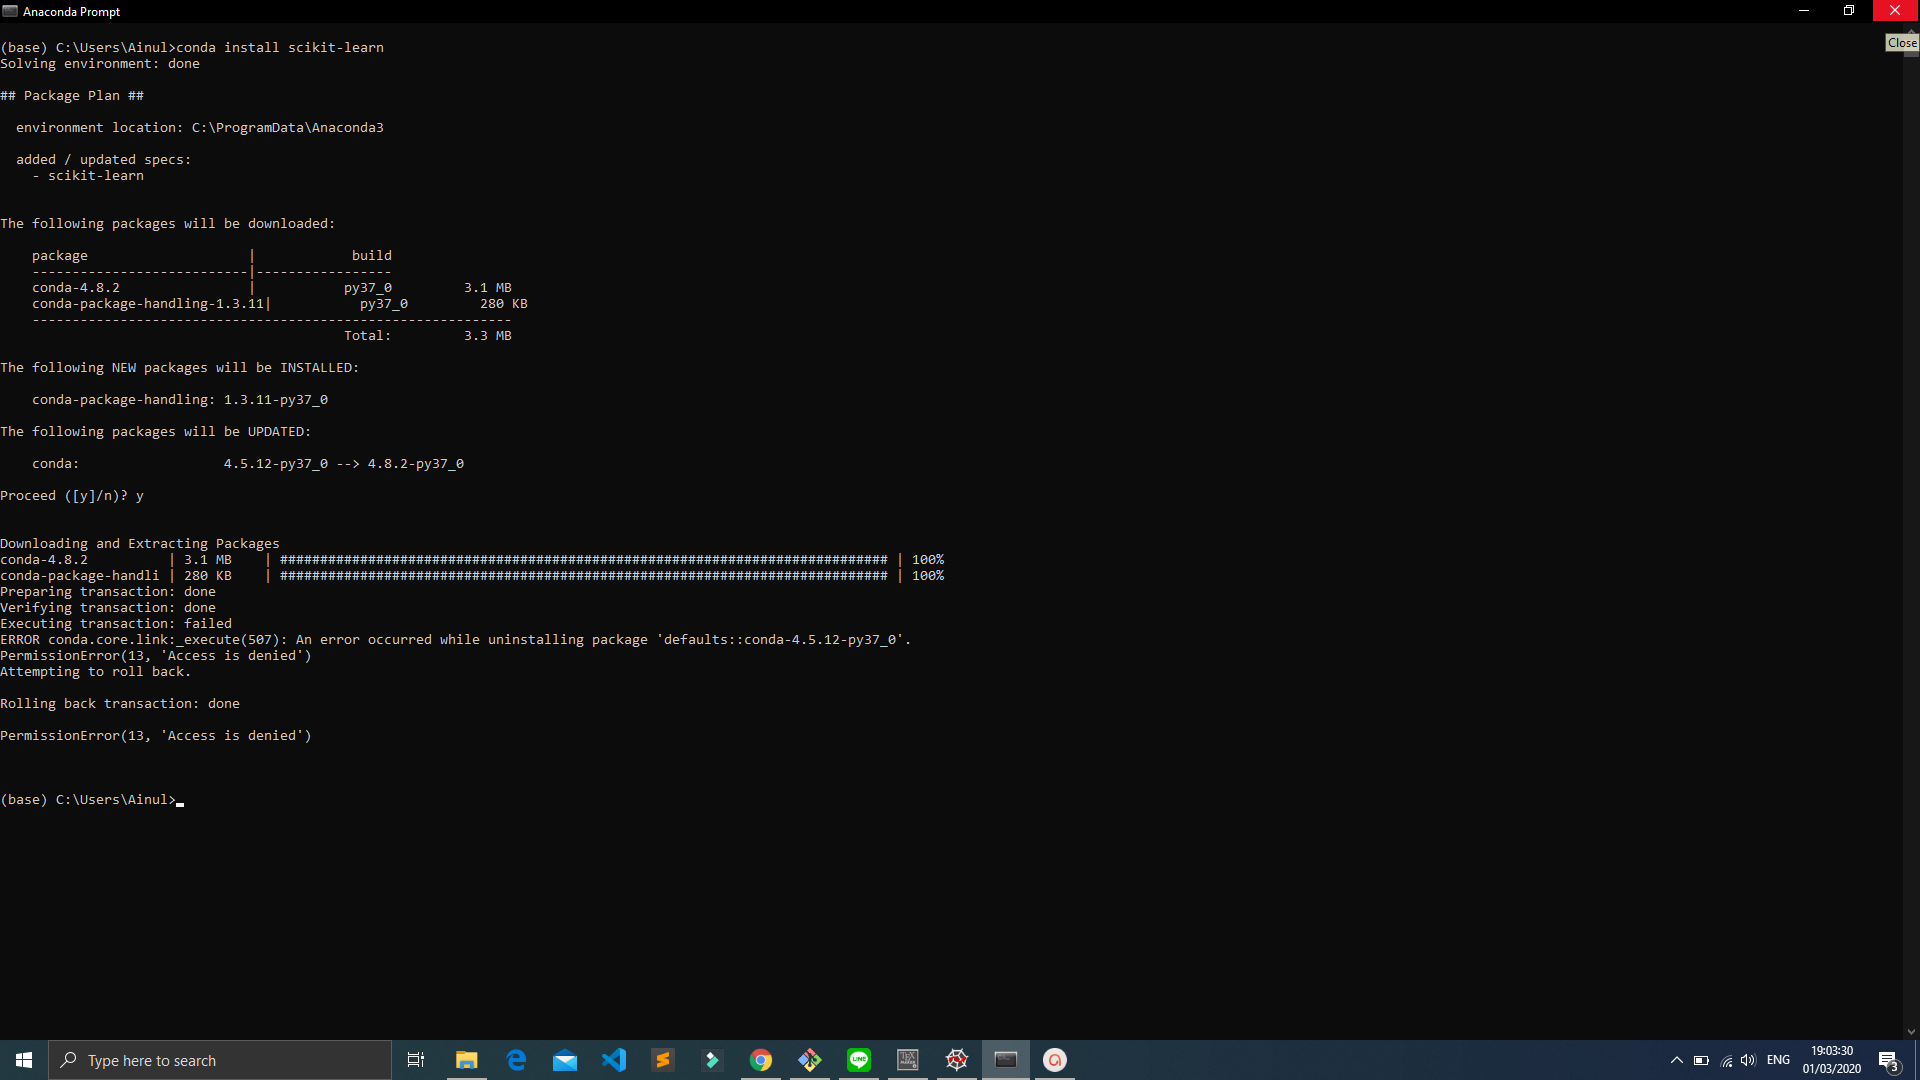
\includegraphics[width=4cm]{figures/1174073/1/1.png}
		\centering
		\caption{Instalasi Package Scikit Learn}
	\end{figure}
	\begin{figure}[H]
		\includegraphics[width=4cm]{figures/1174073/1/2.png}
		\centering
		\caption{Isi Variabel Explorer}
	\end{figure}
	\item Mencoba Loading an example dataset, menjelaskan maksud dari tulisan tersebut dan mengartikan           		  per baris
	\hfill\break
	\lstinputlisting[firstline=7, lastline=11]{src/1174073/1/1174073.py}
	\item Mencoba Learning and predicting, menjelaskan maksud dari tulisan tersebut dan mengartikan per  			  baris
	\hfill\break
	\lstinputlisting[firstline=13, lastline=22]{src/1174073/1/1174073.py}
	\item  Mencoba Model persistence, menjelaskan maksud dari tulisan tersebut dan mengartikan per baris
	\hfill\break
	\lstinputlisting[firstline=25, lastline=34]{src/1174073/1/1174073.py}
	\item Mencoba Conventions, menjelaskan maksud dari tulisan tersebut dan mengartikan per baris
	\hfill\break
	\lstinputlisting[firstline=37, lastline=48]{src/1174073/1/1174073.py}
\end{enumerate}

\subsection{Penanganan Error}
\begin{enumerate}
	\item ScreenShoot Error
	\begin{figure}[H]
		\includegraphics[width=4cm]{figures/1174073/1/error/1.png}
		\centering
		\caption{Import Error}
	\end{figure}

	\item Tuliskan Kode Error dan Jenis Error
	\begin{itemize}
		\item Import Error
	\end{itemize}
	\item Cara Penangan Error
	\begin{itemize}
		\item Import Error
		\hfill\break
		Dengan Menginstall Library Yang Tidak Ditemukan
	\end{itemize}
\end{enumerate}

\subsection{Bukti Tidak Plagiat}
\begin{figure}[H]
	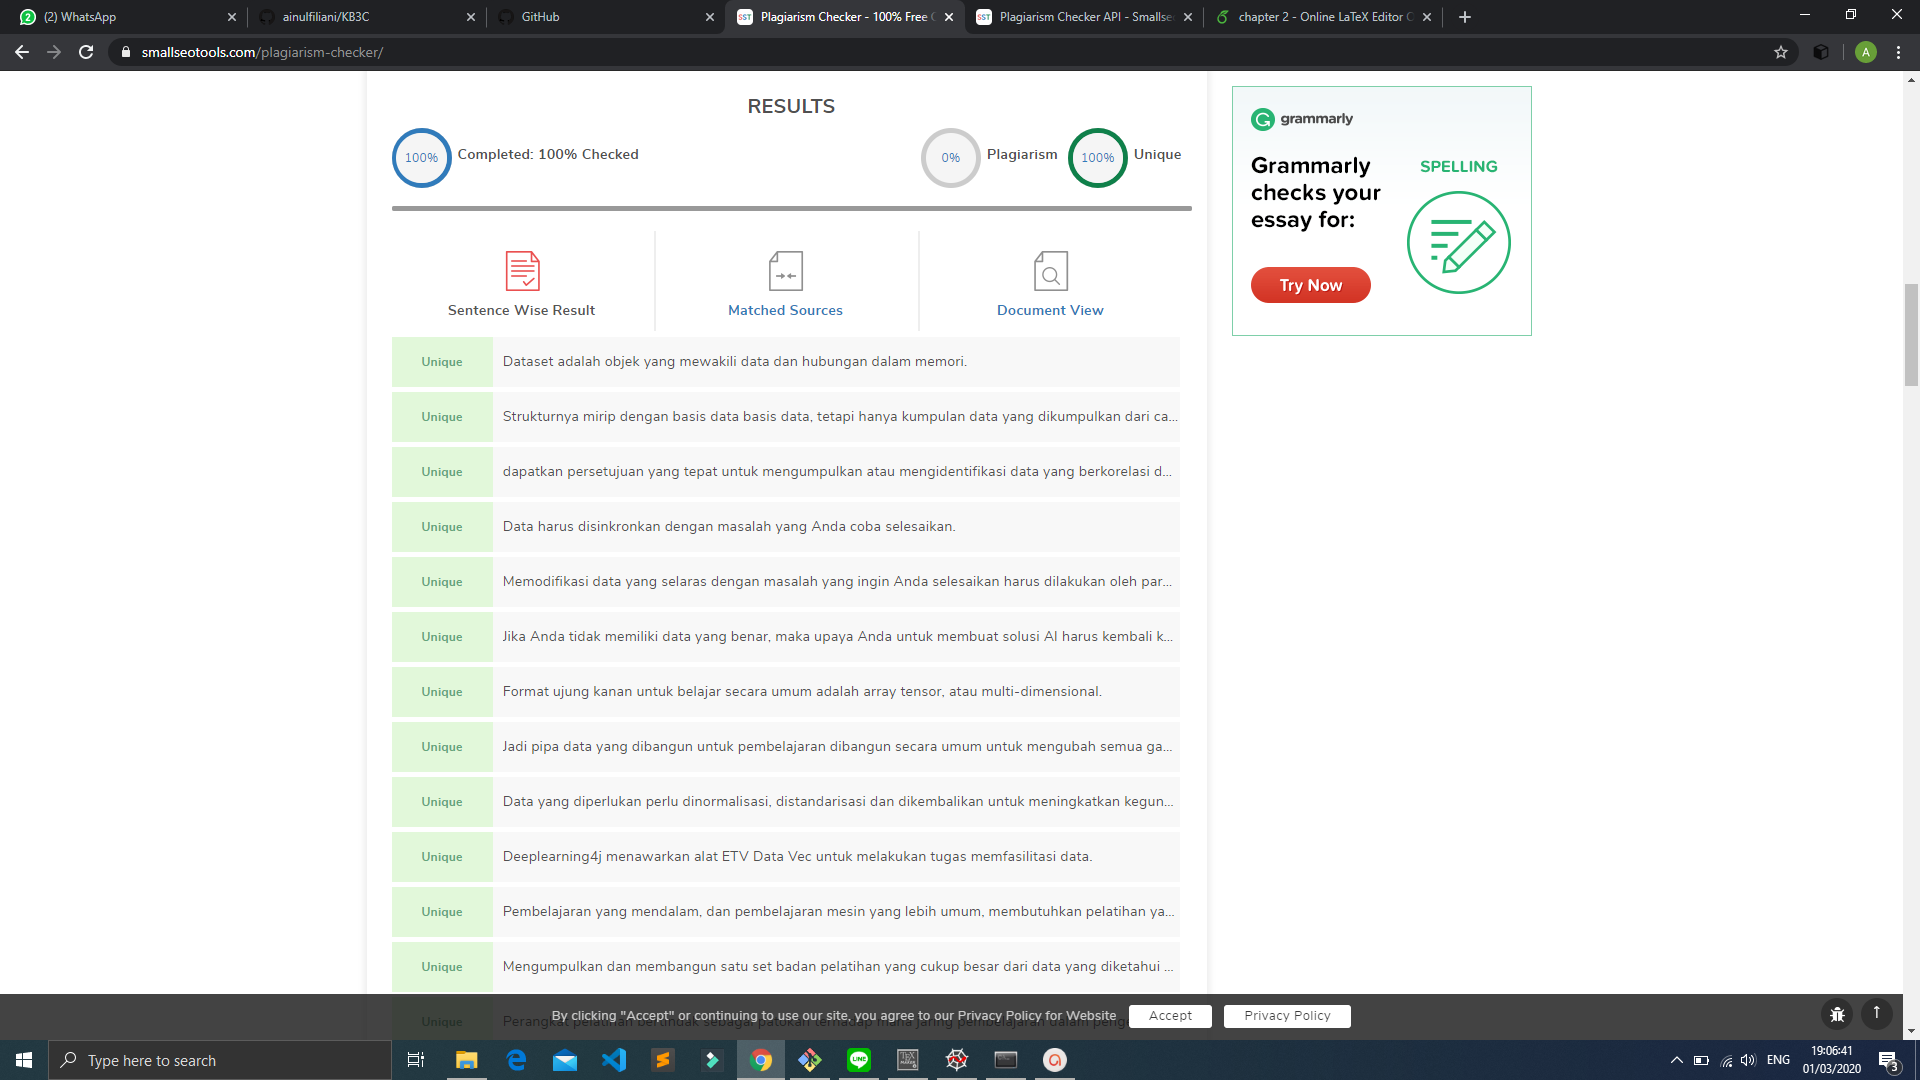
\includegraphics[width=4cm]{figures/1174073/1/plagiat/plagiat.png}
	\centering
	\caption{Bukti Tidak Melakukan Plagiat Chapter 1}
\end{figure}

\subsection{Link Youtube}



%\section{Chandra Kirana Poetra (1174079)}
\subsection{Teori}
\begin{enumerate}
\item Definisi Kecerdasan buatan\\ 
Dalam bidang komputer, Aritificial Intelligence (AI), atau biasa disebut juga sebagai Machine Intelligence merupakan bentuk dari representasi kecerdasan yang dilakukan oleh mesin, hampir mirip seperti bagaimana manusia melakukan kecerdasan. Beberapa sumber mendefinisikan  bahwa bidang yang mempelajari suatu agen kecerdasan merupakan suatu alat yang mengenali lingkungan sekitarnya dan mencoba untuk membuat kesimpulan untuk memaksimalkan kemungkinan tingkat keberhasilan dari pencapaian yang ingin dituju.

\item Sejarah dan Perkembangan Kecerdasan Buatan
\begin{itemize}
\item Pada tahun 1943, pekerjaan pertama yang dikenal sebagai AI telah dilakukan oleh Warren McCulloch dan juga Walter Pits yang dinamakan sebagai artificial neurons
\item Pada tahun 1955, Allen Newell dan Herbert A. Simon membuat program kecerdasan buatan pertama yang dinamakan Logic Theorist
\item Pada tahun 1972, robot pertama dibuat di jepang dengan nama Wabot-1 dengan kecerdasan buatan
\item Pada tahun 1980, muncul bidang baru dari kecerdasan buatan yaitu Expert System yang membantu dalam pemberian keputusan
\item Tahun 1997, IBM deep blue mengalahkan juara catur dunia Gary Kasparov dan menjadi komputer pertama yang mengalahkannya
\item Tahub 2006, perusahaaan sudah mulai menerapkan kecerdasan buatan pada produknya seperti Netflix dan Twitter.
\item Tahun 2018,  	Project Debater dari IBM melakuakn debat tentang topik yang kompleks dan berakhir dengan hasil memuaskan
\end{itemize}

\item Definisi Supervised Learning\\
Supervised Learning adalah proses untuk melatih mesin secara input dan output melalui contoh nyata secara langsung

\item Klasifikasi Supervised Learning
\begin{itemize}
\item Support Vector Machines
\item linear regression
\item logistic regression
\item naive Bayes
\item linear discriminant analysis
\item decision trees
\item k-nearest neighbor algorithm
\item Neural Networks (Multilayer perceptron)
\item Similarity learning
\end{itemize}

\item Regresi dan Unsupervised Learning\\
Regresi adalah suatu proses statistikal yang mengestimasi hubungan antara variable satu dengan variable yang lainnya.

Unsupervised Learning adalah bentuk dari machine learning yang mencari bentuk atau hubungan dari data set yang tidak mempunyai label dengan bantuan yang minimal dari manusia.

\item Dataset\\
Dataset adalah koleksi suatu data

\item Training Set\\
Training Set merupakan data yang digunakan untuk keperluan pembelajaran yang biasanya digunakan oleh machine learning

\item Testing Set\\
Testing set adalah data yang real yang digunakan untuk melatih machine learning

\end{enumerate}

\subsection{Instalasi}
\begin{enumerate}
	\item Instalasi Library scikit dari a naconda, mencoba kompilasi dan uji coba ambil contoh kode dan lihat variabel explorer
	\hfill\break
	\begin{figure}[H]
		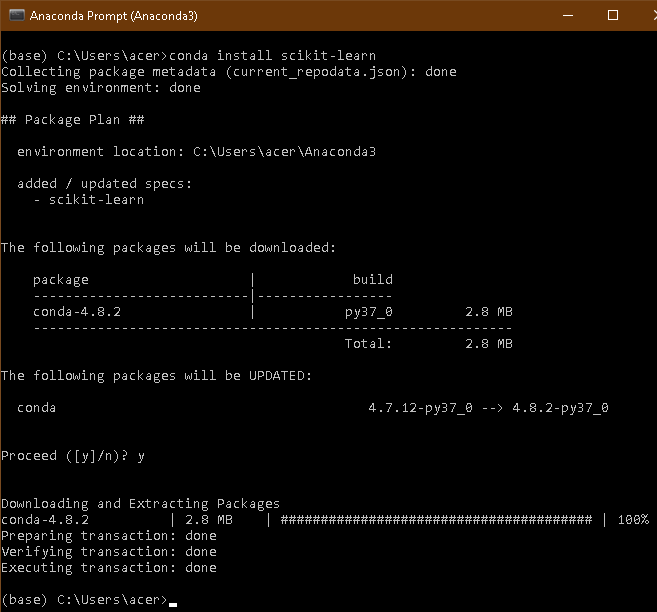
\includegraphics[width=4cm]{figures/1174079/1/1.png}
		\centering
		\caption{Instalasi Package Scikit Learn}
	\end{figure}
	\begin{figure}[H]
		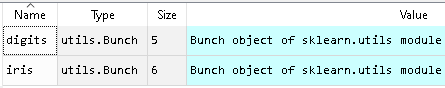
\includegraphics[width=4cm]{figures/1174079/1/2.png}
		\centering
		\caption{Isi Variabel Explorer}
	\end{figure}
	\item Mencoba Loading an example dataset, menjelaskan maksud dari tulisan tersebut dan mengartikan per baris
	\hfill\break
	\lstinputlisting[firstline=2, lastline=7]{src/1174079/1/1174079.py}
	\item Mencoba Learning and predicting, menjelaskan maksud dari tulisan tersebut dan mengartikan perbaris
	\hfill\break
	\lstinputlisting[firstline=9, lastline=28]{src/1174079/1/1174079.py}
	\item  Mencoba Model persistence, menjelaskan maksud dari tulisan tersebut dan mengartikan per baris
	\hfill\break
	\lstinputlisting[firstline=30, lastline=48]{src/1174079/1/1174079.py}
	\item Mencoba Conventions, menjelaskan maksud dari tulisan tersebut dan mengartikan per baris
	\hfill\break
	\lstinputlisting[firstline=50, lastline=72]{src/1174079/1/1174079.py}
\end{enumerate}

\subsection{Penanganan Error}
\begin{enumerate}
	\item ScreenShoot Error
	\begin{figure}[H]
		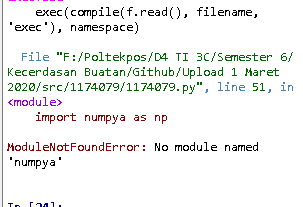
\includegraphics[width=4cm]{figures/1174079/1/error.PNG}
		\centering
		\caption{No Module Named Numpya}
	\end{figure}

	\item Tuliskan Kode Error dan Jenis Error
	\begin{itemize}
		\item ModuleNotFoundError
	\end{itemize}
	\item Cara Penangan Error
	\begin{itemize}
		\item ModuleNotFoundError
		\hfill\break
		Mengecek Typo dan menulis kembali library yang akan diimport
	\end{itemize}
\end{enumerate}

\subsection{Bukti Tidak Plagiat}
\begin{figure}[H]
	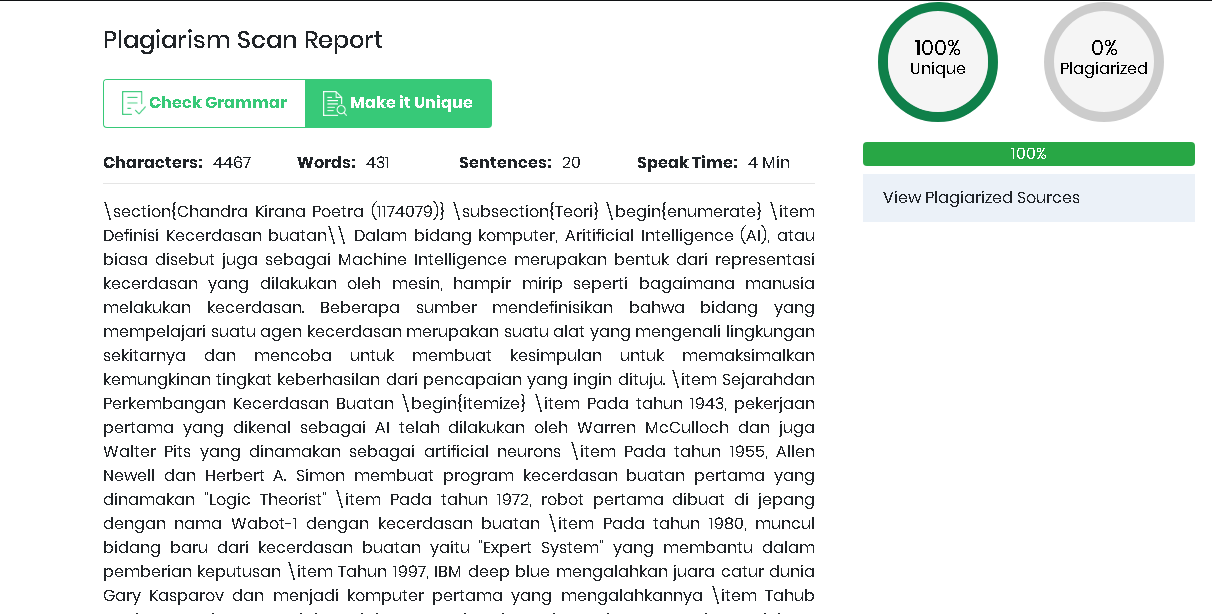
\includegraphics[width=4cm]{figures/1174079/1/plagiarism.PNG}
	\centering
	\caption{Bukti Tidak Melakukan Plagiat Chapter 1}
\end{figure}

\subsection{Link Youtube}
https://youtu.be/nPua0lRXjO8

%\section{D. Irga B. Naufal Fakhri}
\subsection{Teori}
\subsubsection{Definisi Kecerdasan Buatan}

Kecerdasan Buatan atau yang sering disebut AI (Artificial Intelligence) merupakan suatu cabang didalam bisnis sains dan komputer sains yang didalamnya membahas tentang bagaimana caranya untuk membuat sebuah komputer dengan kemampuan atau kepintaran layaknya atau mirip dengan yang dimiliki manusia. 
Contohnya, bagaimana komputer bisa berkomunikasi dengan pengguna baik menggunakan kata, suara ataupun yang lainnya. 
Dengan kemampuan ini, diharapkan komputer dapat mengambil keputusan dengan sendirinya untuk memecahkan berbagai kasus yang ditemuinya kemudian itulah yang disebut dengan kecerdasan buatan. 
Kecerdasan buatan adalah kemampuan komputer digital atau robot yang dikendalikan konputer untuk melakukan tugas yang umumnya dikaitkan dengan sesuatu yang cerdas. Istilah ini sering diterapkan pada proyek pengembangan sistem yang diberkahi dengan karakteristik proses intelektual manusia, seperti kemampuan untuk berpikir, menemukan makna, menggeneralisasi, atau belajar dari pengalaman masa lalu.

Kecerdasan Buatan (AI) merupakan salah satu bidang yang sangat berhubungan dengan memanfaatkan mesin (komputer) untuk memecahkan suatu masalah atau persoalan yang rumit dengan cara yang lebih mudah dimengerti oleh manusia. Kecerdasan Buatan (AI) yang semakin canggih yang mampu menambahkan pengetahuannya dengan cara melakukan banyak testing dan perkembangan dari target yang di analisa. Contoh dari kecerdasan buatan yang paling terkenal saat ini adalah Google Assistant, Alexa dan Siri. Google Assisntant, Alexa dan Siri sangat dikenal karena penggunaannya yang mudah oleh user untuk menemukan berbagai hal atau membuatnya untuk melakukan sesuatu terhadap smartphone atau smarthome anda dan contohnya masih banyak lagi.

\subsubsection{Sejarah Kecerdasan Buatan}

Kecerdasan Buatan (Artificial intelligence) mulai dibentuk sejak adanya komputer modern yang diperkirakan terjadi pada tahun 1940 dan 1950. Ilmu pengetahuan kecerdasan buatan ini dikhususkan dalam perancangan otomatisasi tingkah laku cerdas dalam sistem kecerdasan komputer. 

Pada awal 50-an, studi tentang “mesin berpikir” memiliki berbagai nama seperti cybernetics, teori automata, dan pemrosesan innformasi. 
Pada tahun 1956, para ilmuan jenius seperti Alan Turing, Norbert, Wiener, Claude Shannon dan Warren McCullough telah bekerja secara independen dibidang cybernetics, matematika, algoritma dan teori jaringan. Namun, seprang ilmuan komputer dan kognitif John McCarthy adalah orang yang dating dengan ide untuk bergabung dengan upaya penelitian terpisah ini kedalam satu bidang yang akan mempelajari topic baru untuk imajinasi manusia yaitu kecerdasan buatan. Dia adalah orang yang menciptakan istilah tersebut dan kemudian mendirikan laboratorium Kecerdasan Buatan di MIT dan Stan ford.
Pada tahun 1956, McCarthy yang sama mendirikan Konferensi Dartmouth di Hanover, New Hampshire. Peneliti terkemuka dalam teori kompleksitas, simulasi bahasa, hubungan antara keacakan dan pemikiran kreatif, jaringan saraf diundang. Tujuan dari bidang penelitian yang baru dibuat adalah untuk mengembangkan mesin yang dapat mensimulasikan setiap aspek kecerdasab. Itulah sebabnya Konferensi Dartmouth 1956 dianggap sebagai kelahiran Kecerdasan Buatan. Sejak saat itu, Kecerdasa Buatan telah hidup melalui decade kemuliaan dan cemoohan, yang dikenal luas sebagai musim panas dan musim dingin AI. Musim panasnya ditandai dengan optimism dan dana besar, sedangkan musim dinginnya dihadapkan dengan pemotongan dana, ketidakkpercayaan dan pesimisme.

\subsubsection{Perkembangan Kecerdasan Buatan}

Teknologi Artificial Intelligence semakin ramai dibahas dalam berbagai diskusi teknologi di seluruh dunia.Menurut kebanyakan orang, pekerjaan seperti kasir, operator telepon, pengendara truk, dan lainnya sangat berpeluang besar untuk tergantikan oleh Artificial Intelligence. Mengapa terjadi hal demikian? dikarenakan memang bahwa AI lebih ungul dalam hal kinerja, fitur dan lain sebagainya. Namun, dalam beberapa aspek memang pekerja manusia masih unggul dibandingkan AI itu sendiri. Para generasi muda yang ada di dunia terutama di daerah Asia terlihat sudah memahami fungsi dan efek dari AI dalam kehidupan kita sehari-hari. Berdasarkan survei yang dilakukan oleh Microsoft, terdapat 39 persen responden yang mempertimbangkan untuk menggunakan mobil tanpa pengemudi dan 36 persen lainnya setuju bahwa robot masa depan dengan software untuk beroperasi mampu meningkatkan produktivitas. Dari survey tersebut kita sebagai pengguna AI harus lebih bijaksana dalam pengembangan dan penggunaan dari AI sehingga tanpa memberikan efek samping terhadap etos kerja dan keseharian kita sebagai pengguna dalam kehidupan sehari-hari.

AI Summer 1 (1956-1973) KOnferensi Dartmounth diikuti oleh 17 tahun kemajuan luar biasa. Proyek penelitian yang dilakukan di MIT, universitas di Edinburgh, Stanford dan Carnegie Mellon menerima dana besar-besaran, yang akhirnya membuahkan hasil. Selama tahun-tahun itulah komputer pemrograman mulai melakukan masalah aljabar, membuktikan teorema geometris, memahami dan menggunakan sintaks dan tata bahasa Inggris. Terlepas dari ditinggalkannya koneksionisme dan terjemahan mesin yang gagal, yang menunda penelitian Natural Language Processing (NLP) selama bertahun-tahun, banyak prestasi dari masa lalu yang membuat sejarah. Berikut ini beberapa diantaranya : Pelopor pembelajaran mesin, Ray Solomonoff meletakkan dasar-dasar teori metematika AI, memperkenalkan metode Bayesian universal untuk inferensi dan preddiksi induktif Thomas Evans menciptakan program ANALOGI heuristik, yang memungkinkan komputer memecahkan masalah geometri-analogi Unimation, perusahaan robotika pertma didunia, menciptakan robot industri Unimate, yang bekerja pada jalur perakitan modil Genenral Motors. Joseph Weizenbaum membangun ELIZA-program interaktif yang dapat membawa percakapan dalam bahasan Inggris tentang topik apapun. Ross Quillian menunjukkan jaring semanik, sedangkan Jaime Carbonell (Sr.) mengembangkan Cendikia-program interaktif untuk instruksi yang dibantu komputer berdasarkan jaring semantik. Edward Feigenbaum dan Julian Feldman menerbitkan Computeks and Thought, kumpulan artikel pertama tentang AI.

\subsubsection{Supervised Learning}
Supervised Learning adalah tugas pengumpulan data untuk menyimpulkan fungsi dari data pelatihan berlabel. Data pelatihan terdiri dari serangkaian contoh pelatihan. Dalam supervised learning, setiap contoh adalah pasangan yang terdiri dari objek input (biasanya vektor) dan nilai output yang diinginkan(juga disebut sinyal pengawasan super). Algoritma pembelajaran yang diawasi menganalisis data pelatihan dan menghasilkan fungsi yang disimpulkan, yang dapat digunakan untuk memetakan contoh-contoh baru. Skenario optimal akan memungkinkan algoritma menentukan label kelas dengan benar untuk instance yang tidak terlihat. Ini membutuhkan algoritma pembelajaran untuk menggeneralisasi dari data pelatihan untuk situasi yang tidak terlihat dengan cara yang "masuk akal". Supervised Learning adalah pendekatan dimana sudah terdapat data yang dilatih selain itu juga terdapat variable yang ditargetkan sehingga tujuan dari pendekatan ini yaitu mengelompokkan suatu data ke dta yang sudah ada. Supervised Learning menyediakan algoritma pembelajaran dengan jumlah yang diketahui untuk mendukung penilaian dimasa depan. Chatbots, mobil self-driving, program pengenalan wajah, sistem pakar dan robot adalah beberapa sistem yang dapat menggunakan pembelajaran yang diawasi atau tidak diawasi. Supervised Learning sebagian besar terkait dengan AI berbasis pengambilan tetapi mereka juga mungkin mampu menggunakan model pembelajaran generatif. Data pelatihan untuk pembelajaran yang diawasi mencakup serangkaian contoh dengan subjek input berpasangan dan output yang diinginkan (yang juga disebut sebagai sinyal pengawasan).

Dalam pembelajaran yang diawasi untuk pemrosesan gambar, misalnya sistem AI mungkin dilengkapi dengan gambar berlabel kendaraan dalam ketegori seperti mobil dan truk. Setelah jumlah pengamatan yang cukup, sistem harus dapat membedakan antara dan mengkategorikan gambar yang tidak berlabel, dimana waktu pelatihan dapat dikatakan lengkap. Model Supervised Learning memiliki beberapa keunggulan dibandingkan pendekatan tanpa pengawasan, tetapi mereka juga memiliki keterbatasan. Sistem lebih cenderung membuat penilaian bahwa manusia dapat berhubungan, misalnya karena manusia telah memberikan dasar untuk keputusan. Namun, dalam kasus metode berbasis pengambilan, Supervised Learning mengalami kesulitan dalam menangani informaasi baru. Jika suatu sistem dengan kategori untuk mobil dan truk disajikan dengan sepeda, misalnya ia harus salah dikelompokkan dalam satu kategori ata yang lain. Namun. jika sistem AI bersifat generatif, ia mungkin tidak tahu apa sepeda itu tetapi akan dapat mengenalinya sebagai milik kategori yang terpisah.

\subsubsection{Klasifikasi}
Klasifikasi adalah pembagian sesuatu menurut kelas-kelas ( class ). Menurut Ilmu Pengetahuan, Klasifikasi merupakan proses pengelompokkan benda berdasarkan ciri-ciri persamaan dan juga perbedaan. Dalam masalah klasifikasi, kami mencoba memprediksi sejumlah nilai terpisah. Label (y) umumnya datang dalam bentuk kategorikal dan mewakili sejumlah kelas. Dalam pembelajaran mesin dan statistik, klasifikasi adalah pendekatan pembelajaran yang diawasi di mana program komputer belajar dari input data yang diberikan kepadanya dan kemudian menggunakan pembelajaran ini untuk mengklasifikasikan pengamatan baru. Kumpulan data ini mungkin hanya bersifat dua kelas (seperti mengidentifikasi apakah orang tersebut berjenis kelamin laki-laki atau perempuan atau bahwa surat itu spam atau bukan-spam) atau mungkin juga multi-kelas. Beberapa contoh masalah klasifikasi adalah: pengenalan ucapan, pengenalan tulisan tangan, identifikasi metrik, klasifikasi dokumen dll.

\subsubsection{Regresi}
Regresi adalah metode analisis statistik yang digunakan untuk melihat pengaruh antara dua ataupun lebih variabel. Regresi adalah membahas masalah ketika variabel output adalah nilai riil atau berkelanjutan, seperti "gaji" atau "berat". Banyak model yang berbeda dapat digunakan makan, yang paling sederhana adalah regresi linier. Ia mencoba untuk menyesuaikan data dengan hyper-plane terbaik yang melewati poin.

\subsubsection{Unsupervised Learning}
Unsupervised Learning berbeda dengan Supervised Leraning. Perbedaannya ialah unsupervised learning tidak memiliki data latih, sehingga dari data yang ada kita mengelompokan data tersebut menjadi 2 ataupun 3 bagian dan seterusnya. Unsupervised Learning adalah pelatihan algoritma kecerdasan buatan (AI) menggunakan informasi yang tidak diklasifikasikan atau diberi label dan memungkinkan algoritma untuk bertindak atas informasi tersebut tanpa bimbingan. Dalam Unsupervised Learning, sistem AI dapat mengelompokkan informasi yang tidak disortir berdasarkan persamaan dan perbedaan meskipun tidak ada kategori yang disediakan.

Dalam Unsupervised Learning, sistem AI disajikan dengan data yang tidak berlabel, tidak terkategorisasi dan algoritma sistem bekerja pada data tanpa pelatihan sebelumnya. Outputnya tergantung pada algoritma kode. Menundukkan suatu sistem pada Unsupervised Learning adalah salah satu cara untuk menguji AI. Algoritma Unsupervised Learning dapat melakukan tugas pemrosesan yang lebih kompleks daripada sistem pembelajaran yang
diawasi. Namun, pembelajaran tanpa pengawasan bisa lebih tidak terduga daripada model alternatif. Sementara Unsupervised Learningi mungkin, misalnya, mencari tahu sendiri cara memilah kucing dari anjing, mungkin juga menambahkan kategori yang tidak terduga dan tidak diinginkan untuk menangani breed yang tidak biasa, membuat kekacauan bukannya keteraturan


\subsubsection{Data Set}
Dataset adalah objek yang merepresentasikan data dan juga relasi yang ada di memory. Strukturnya mirip dengan data di database, namun bedanya
dataset berisi koleksi dari data table dan data relation. mendapatkan data yang tepat berarti mengumpulkan atau mengidentifikasi data yang berkorelasi dengan hasil yang ingin Anda prediksi; yaitu data yang berisi sinyal tentang peristiwa yang Anda pedulikan. Data harus diselaraskan dengan masalah yang Anda coba selesaikan. Gambar kucing tidak terlalu berguna ketika Anda sedang membangun sistem identifikasi wajah. Memverifikasi bahwa data selaras dengan masalah yang ingin Anda selesaikan harus dilakukan oleh ilmuwan data. Jika Anda tidak memiliki data yang tepat, maka upaya Anda untuk membangun solusi AI harus kembali ke tahap pengumpulan data. Format ujung kanan untuk pembelajaran dalam umumnya adalah tensor, atau array multi-dimensi. Jadi jalur pipa data yang dibangun untuk pembelajaran mendalam umumnya akan mengkonversi semua data - baik itu gambar, video, suara, suara, teks atau deret waktu  menjadi vektor dan tensor yang dapat diterapkan operasi aljabar linier. Data itu seringkali perlu dinormalisasi, distandarisasi dan dibersihkan untuk meningkatkan kegunaannya, dan itu semua adalah langkah dalam ETL pembelajaran mesin. Deeplearning4j menawarkan alat ETV DataVec untuk melakukan tugas-tugas pemrosesan data tersebut.

Pembelajaran yang dalam, dan pembelajaran mesin yang lebih umum, membutuhkan pelatihan yang baik agar bekerja dengan baik. Mengumpulkan dan membangun set pelatihan  badan yang cukup besar dari data yang diketahui  membutuhkan waktu dan pengetahuan khusus domain tentang di mana dan bagaimana mengumpulkan informasi yang relevan. Perangkat pelatihan bertindak sebagai tolok ukur terhadap mana jaring pembelajaran dalam dilatih. Itulah yang mereka pelajari untuk direkonstruksi sebelum mereka melepaskan data yang belum pernah mereka lihat sebelumnya. Pada tahap ini, manusia yang berpengetahuan luas perlu menemukan data mentah yang tepat dan mengubahnya menjadi representasi numerik yang dapat dipahami oleh algoritma pembelajaran mendalam, tensor. Membangun set pelatihan, dalam arti tertentu, pra-pra pelatihan. Set pelatihan yang membutuhkan banyak waktu atau keahlian dapat berfungsi sebagai keunggulan dalam dunia ilmu data dan pemecahan masalah. Sifat keahlian sebagian besar dalam memberi tahu algoritma Anda apa yang penting bagi Anda dengan memilih apa yang masuk ke dalam set pelatihan. Ini melibatkan menceritakan sebuah kisah  melalui data awal yang Anda pilih yang akan memandu jaring pembelajaran mendalam Anda saat mereka mengekstraksi fitur-fitur penting, baik di set pelatihan maupun dalam data mentah yang telah mereka ciptakan untuk dipelajari. Untuk membuat set pelatihan yang bermanfaat, Anda harus memahami masalah yang Anda selesaikan; yaitu apa yang Anda inginkan agar jaring pembelajaran mendalam Anda memperhatikan, di mana hasil yang ingin Anda prediksi.


\subsubsection{Training Set}
Training Set adalah set digunakan oleh algoritma klassifikasi . Dapat dicontohkan dengan : decision tree, bayesian, neural network dll. Semuanya dapat digunakan untuk membentuk sebuah model classifier. Menjalankan pelatihan yang diatur melalui jaringan saraf mengajarkan pada net
cara menimbang berbagai fitur, menyesuaikan koefisien berdasarkan kemungkinan mereka meminimalkan kesalahan dalam hasil Anda. Koefisien-koefisien tersebut, juga dikenal sebagai parameter, akan terkandung dalam tensor dan bersama-sama mereka disebut model, karena mereka mengkodekan model data yang mereka latih. Mereka adalah takeaways paling penting yang akan Anda dapatkan dari pelatihan jaringan saraf.


\subsubsection{Testing Set}
Testing Set adalah set yang digunakan untuk mengukur sejauh mana classifier berhasil melakukan klasifikasi dengan benar. Ini berfungsi sebagai meterai persetujuan, dan Anda tidak menggunakannya sampai akhir. Setelah Anda melatih dan mengoptimalkan data Anda, Anda menguji jaringan saraf Anda terhadap pengambilan sampel acak akhir ini. Hasil yang dihasilkannya harus memvalidasi bahwa jaring Anda secara akurat mengenali gambar, atau mengenalinya setidaknya [x] dari jumlah tersebut. Jika Anda tidak mendapatkan prediksi yang akurat, kembalilah ke set pelatihan, lihat hyperparameter yang Anda gunakan untuk menyetel jaringan, serta kualitas data Anda dan lihat teknik pra-pemrosesan Anda.

\subsection{Praktek}
\subsubsection{Instalasi library scikit dari anaconda, mencoba kompilasi dan uji coba ambil contoh kode dan lihat variabel explorer}
\begin{enumerate}

\item Pastikan anda telah menginstall anaconda lalu buka aplikasi Anaconda Prompt

\item Lalu pastikan anda telah menginstall python

\item Pada Anaconda Prompt install scikit dengan cara conda install scikit-learn
\begin{figure}[H]
	\begin{center}
   	 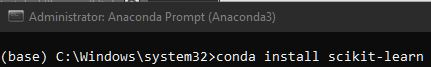
\includegraphics[width=10cm]{figures/1174066/1/1.jpg}
   	 \caption{Instalasi Scikit Dari Anaconda Prompt}	
	\end{center}
\end{figure}

\item Lalu tulis kode yang ada dibawah ini dan run menggunakan spyder
\lstinputlisting[firstline=1, lastline=4]{src/1174066/1/contoh.py}
\begin{figure}[H]
	\begin{center}
   	 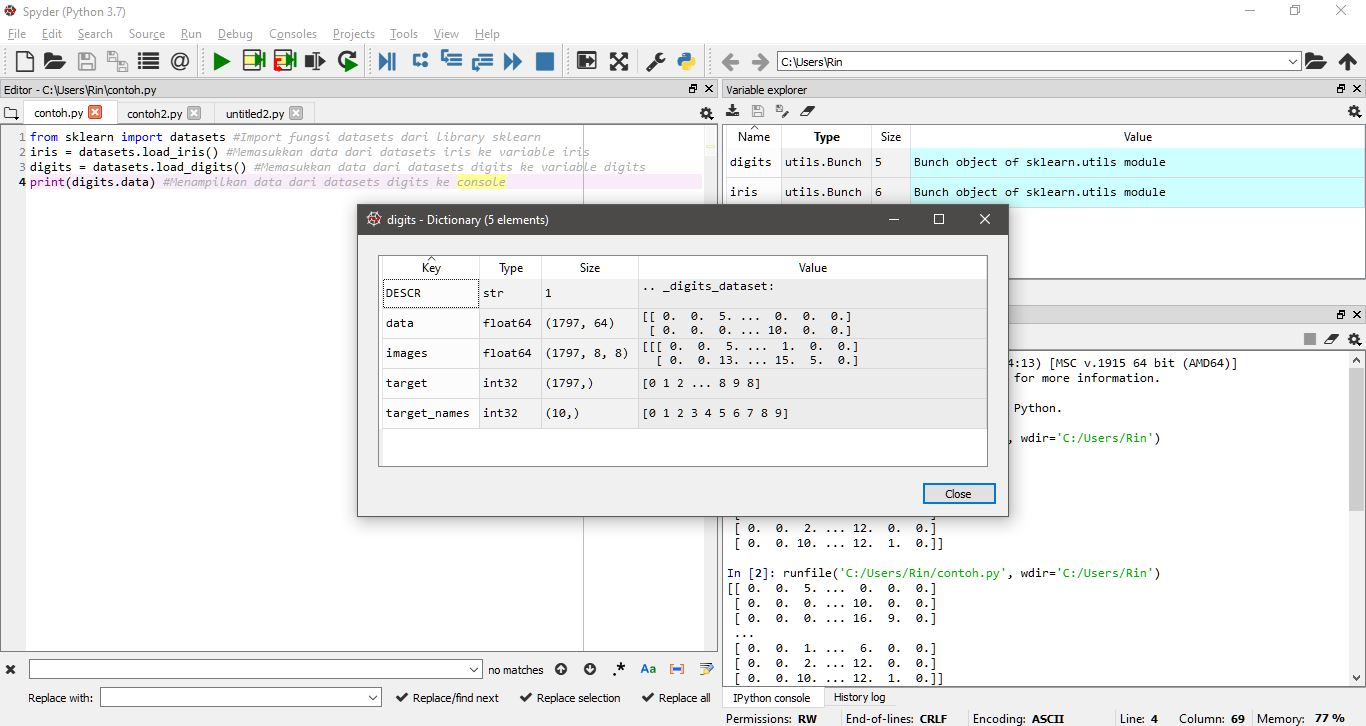
\includegraphics[width=10cm]{figures/1174066/1/2.jpg}
   	 \caption{Running Kode dari Spyder dan Hasil Variable Explorer}	
	\end{center}
\end{figure}
\end{enumerate}

\subsubsection{Loading an example dataset}
\begin{figure}[H]
	\begin{center}
   	 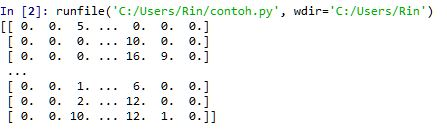
\includegraphics[width=10cm]{figures/1174066/1/3.jpg}
   	 \caption{Running Loading an example dataset dari Spyder}	
	\end{center}
\end{figure}

\begin{itemize}
\item Import fungsi datasets dari library sklearn
\lstinputlisting[firstline=1, lastline=1]{src/1174066/1/contoh.py}

\item Memasukkan data dari datasets iris ke variable iris
\lstinputlisting[firstline=2, lastline=2]{src/1174066/1/contoh.py}

\item Memasukkan data dari datasets digits ke variable digits
\lstinputlisting[firstline=3, lastline=3]{src/1174066/1/contoh.py}

\item Menampilkan data dari datasets digits ke console
\lstinputlisting[firstline=4, lastline=4]{src/1174066/1/contoh.py}
\begin{figure}[H]
	\begin{center}
   	 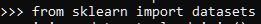
\includegraphics[width=10cm]{figures/1174066/1/5.jpg}
   	 \caption{Hasil Running kode loading an example dataset}	
	\end{center}
\end{figure}
\end{itemize}

\subsubsection{Learning and predicting}
\begin{itemize}
\item Buka Anaconda Prompt
\begin{figure}[H]
	\begin{center}
   	 
\includegraphics[width=10cm]{figures/1174066/1/anaconda.jpg}
   	 \caption{Anaconda Prompt}	
	\end{center}
\end{figure}

\item Lalu kita import datasets dari sklearn seperti dibawah ini
\begin{figure}[H]
	\begin{center}
   	 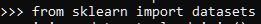
\includegraphics[width=10cm]{figures/1174066/1/5.jpg}
   	 \caption{Menggunakan datasets}	
	\end{center}
\end{figure}

\item lalu kita mendefisisikan iris dan digits menjadi variable
\begin{figure}[H]
	\begin{center}
   	 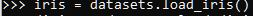
\includegraphics[width=10cm]{figures/1174066/1/6.jpg}
   	 \caption{mendefinisikan iris}	
	\end{center}
\end{figure}
\begin{figure}[H]
	\begin{center}
   	 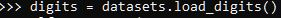
\includegraphics[width=10cm]{figures/1174066/1/7.jpg}
   	 \caption{mendefinisikan digits}	
	\end{center}
\end{figure}

\item Lalu kita import svm dari sklearn yang nantinya digunakan untuk menjadi estimanasi angka kita
\begin{figure}[H]
	\begin{center}
   	 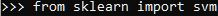
\includegraphics[width=10cm]{figures/1174066/1/4.jpg}
   	 \caption{Menggunakan svm}	
	\end{center}
\end{figure}

\item Lalu, kita definisikan clf sebagai classfier, disini gamma didefinisikan secara manual
\begin{figure}[H]
	\begin{center}
   	 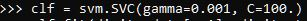
\includegraphics[width=10cm]{figures/1174066/1/8.jpg}
   	 \caption{Mendefinisikan Classifier}	
	\end{center}
\end{figure}

\item Estimator clf (for classifier) pertama kali dipasang pada model. Ini dilakukan dengan melewati training set ke metode fit. Untuk training set, akan menggunakan semua gambar dari set data yang ada, kecuali untuk gambar terakhir, yang dicadangan untuk prediksi. Pada skrip dibawah memilih training set dengan sintaks Python [: -1], yang menghasilkan array baru yang berisi semua kecuali item terakhir dari digits.
\begin{figure}[H]
	\begin{center}
   	 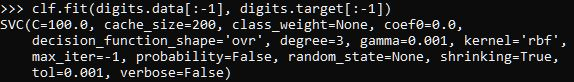
\includegraphics[width=10cm]{figures/1174066/1/9.jpg}
   	 \caption{Memanggil Classifier}	
	\end{center}
\end{figure}

\item Menunnjukkan prediksi angka baru
\begin{figure}[H]
	\begin{center}
   	 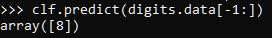
\includegraphics[width=10cm]{figures/1174066/1/10.jpg}
   	 \caption{Prediksi nilai baru}	
	\end{center}
\end{figure}
\end{itemize}
\lstinputlisting[firstline=8 lastline=15]{src/1174066/1/contoh2.py}

\subsubsection{Model Persistance}
Model Persistance
\lstinputlisting[firstline=8 lastline=32]{src/1174066/1/contoh3.py}

\subsubsection{Conversion}
Conversion
\lstinputlisting[firstline=8 lastline=19]{src/1174066/1/contoh4.py}

\subsection{Penanganan Error}

Dari percobaan yang dilakukan di atas, apabila mendapatkan error maka:
\begin{enumerate}

\item Screenshoot Error
\begin{figure}[H]
	\begin{center}
   	 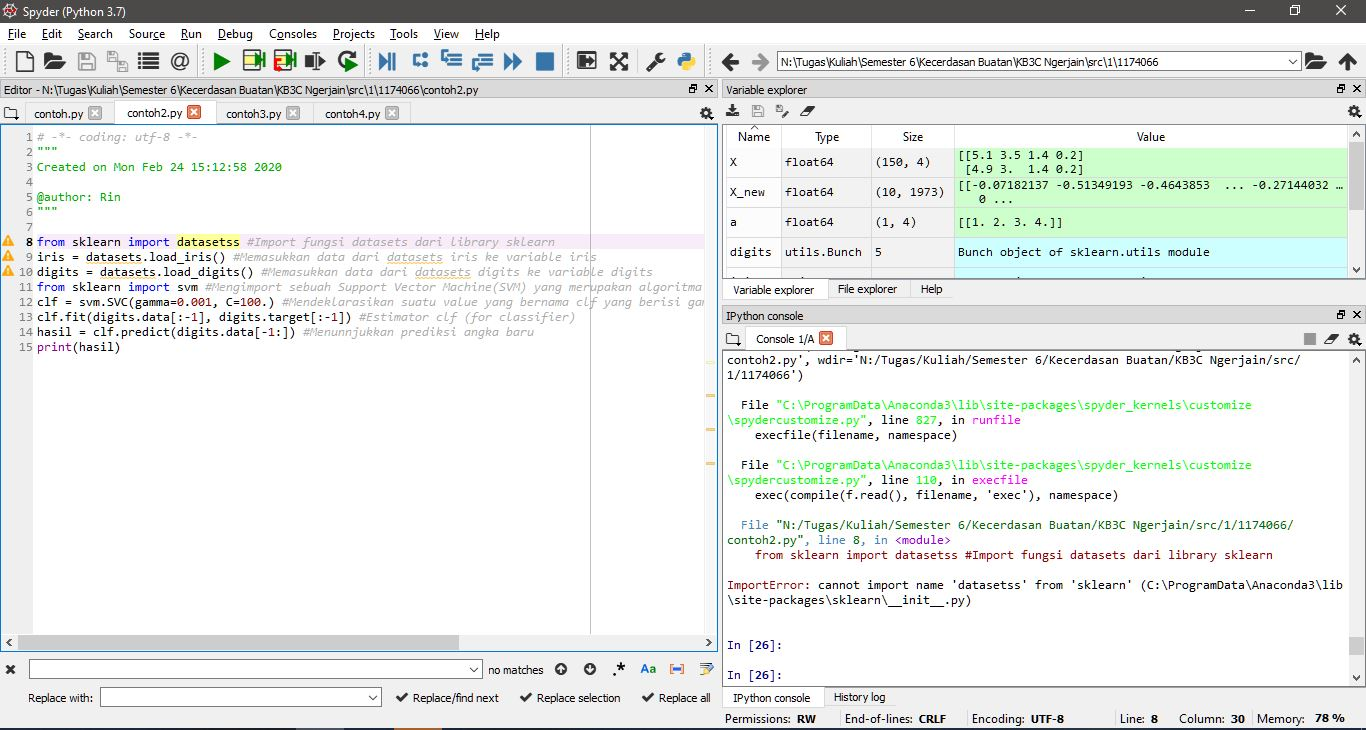
\includegraphics[width=10cm]{figures/1174066/1/error1.jpg}
   	 \caption{ImportError: cannot import name 'datasetss' from 'sklearn'}	
	\end{center}
\end{figure}
	
\item Tuliskan kode eror dan jenis errornya [hari ke 2](10)
\begin{itemize}
\item ImportError
\end{itemize}

\item Solusi pemecahan masalah error tersebut[hari ke 2](10)
\begin{itemize}
\item ImportError

Cek kembali jika ada yang typo
\end{itemize}

\end{enumerate}

\subsection{Bukti Tidak Plagiat}
\begin{figure}[H]
	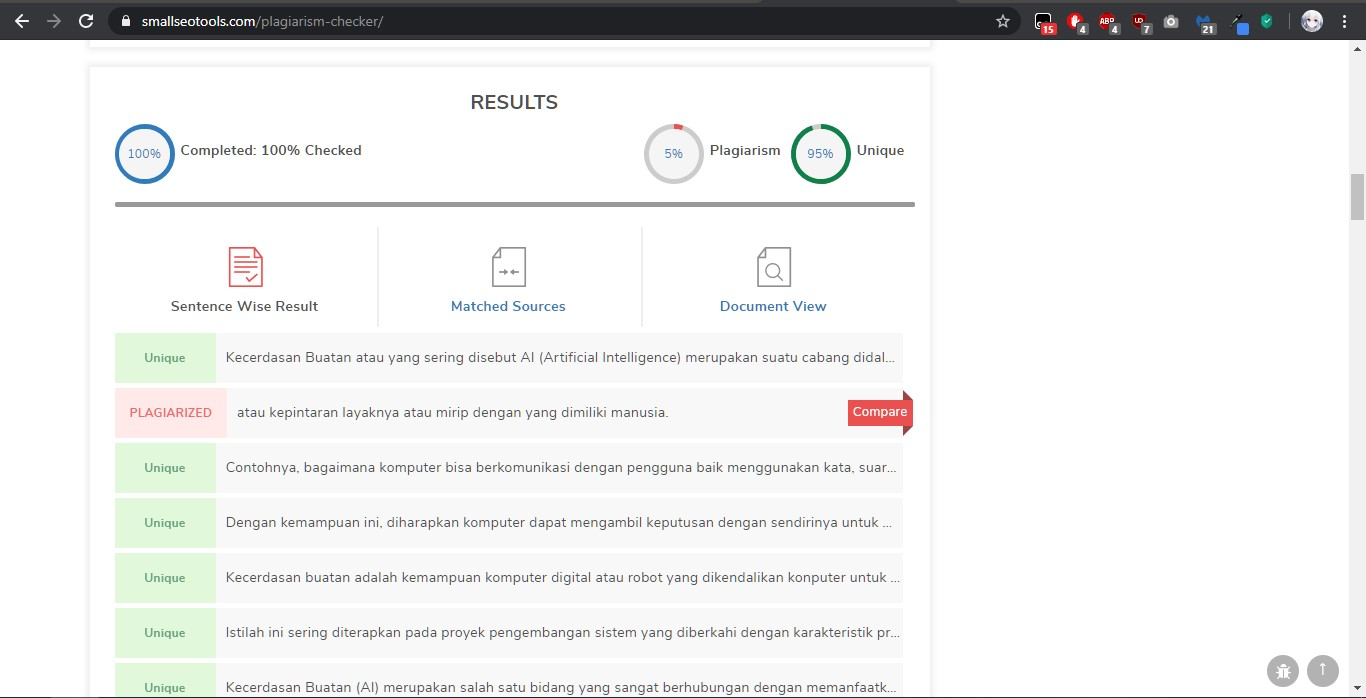
\includegraphics[width=4cm]{figures/1174066/1/plagiat.jpg}
	\centering
	\caption{Bukti Tidak Melakukan Plagiat Chapter 1}
\end{figure}

\subsection{Link Youtube}
https://youtu.be/S8Sj\_vZluUs
%\section{1174087 - Ilham Muhammad Ariq}
\subsection{Teori}
\begin{enumerate}
	\item Definisi Kecerdasan Buatan
		\par Kecerdasan Buatan adalah suatu ilmu yang mempelajari bagaimana cara komputer melakukan sesuatu seperti yang dilakukan oleh manusia. Secara sederhana AI adalah teknik dan ilmu untuk membangun atau membuat suatu mesin menjadi cerdas, terutama pada program komputer. Kecerdasan yang dimaksud yaitu seperti yang dimiliki oleh manusia namun pada mesin akan dibuat cepat dan tepat atau akurat.

\item {Sejarah Kecerdasan Buatan}
    \par Artificial intelligence merupakan inovasi baru di bidang ilmu pengetahuan. Mulai terbentuk sejak adanya komputer modern dan kira-kira terjadi sekitaran tahun 1940 dan 1950. Ilmu pengetahuan komputer ini khusus ditujukan dalam perancangan otomatisasi tingkah laku cerdas dalam sistem kecerdasan komputer. Pada awal 50-an, studi tentang “mesin berpikir” memiliki berbagai nama seperti cybernetics, teori automata, dan pemrosesan innformasi. Pada tahun 1956, para ilmuan jenius seperti Alan Turing, Norbert, Wiener, Claude Shannon dan Warren McCullough telah bekerja secara independen dibidang cybernetics, matematika, algoritma dan teori jaringan. Namun, seprang ilmuan komputer dan kognitif John McCarthy adalah orang yang dating dengan ide untuk bergabung dengan upaya penelitian terpisah ini kedalam satu bidang yang akan mempelajari topic baru untuk imajinasi manusia yaitu kecerdasan buatan. Dia adalah orang yang menciptakan istilah tersebut dan kemudian mendirikan laboratorium Kecerdasan Buatan di MIT dan Stan ford.

    Pada tahun 1956, McCarthy yang sama mendirikan Konferensi Dartmouth di Hanover, New Hampshire. Peneliti terkemuka dalam teori kompleksitas, simulasi bahasa, hubungan antara keacakan dan pemikiran kreatif, jaringan saraf diundang. Tujuan dari bidang penelitian yang baru dibuat adalah untuk mengembangkan mesin yang dapat mensimulasikan setiap aspek kecerdasab. Itulah sebabnya Konferensi Dartmouth 1956 dianggap sebagai kelahiran Kecerdasan Buatan. Sejak saat itu, Kecerdasa Buatan telah hidup melalui decade kemuliaan dan cemoohan, yang dikenal luas sebagai musim panas dan musim dingin AI. Musim panasnya ditandai dengan optimism dan dana besar, sedangkan musim dinginnya dihadapkan dengan pemotongan dana, ketidakkpercayaan dan pesimisme.

    \item{Perkembangan Kecerdasan Buatan}
    \par Teknologi Artificial Intelligence semakin ramai dibahas dalam berbagai diskusi teknologi di seluruh dunia.Menurut kebanyakan orang, pekerjaan seperti kasir, operator telepon, pengendara truk, dan lainnya sangat berpeluang besar untuk tergantikan oleh Artificial Intelligence. Mengapa terjadi hal demikian? dikarenakan memang bahwa AI lebih ungul dalam hal kinerja, fitur dan lain sebagainya. Namun, dalam beberapa aspek memang pekerja manusia masih unggul dibandingkan AI itu sendiri. Para generasi muda yang ada di dunia terutama di daerah Asia terlihat sudah memahami fungsi dan efek dari AI dalam kehidupan kita sehari-hari. Berdasarkan survei yang dilakukan oleh Microsoft, terdapat 39 persen responden yang mempertimbangkan untuk menggunakan mobil tanpa pengemudi dan 36 persen lainnya setuju bahwa robot masa depan dengan software untuk beroperasi mampu meningkatkan produktivitas. Dari survey tersebut kita sebagai pengguna AI harus lebih bijaksana dalam pengembangan dan penggunaan dari AI sehingga tanpa memberikan efek samping terhadap etos kerja dan keseharian kita sebagai pengguna dalam kehidupan sehari-hari.

    AI Summer 1 (1956-1973) KOnferensi Dartmounth diikuti oleh 17 tahun kemajuan luar biasa. Proyek penelitian yang dilakukan di MIT, universitas di Edinburgh, Stanford dan Carnegie Mellon menerima dana besar-besaran, yang akhirnya membuahkan hasil. Selama tahun-tahun itulah komputer pemrograman mulai melakukan masalah aljabar, membuktikan teorema geometris, memahami dan menggunakan sintaks dan tata bahasa Inggris. Terlepas dari ditinggalkannya koneksionisme dan terjemahan mesin yang gagal, yang menunda penelitian Natural Language Processing (NLP) selama bertahun-tahun, banyak prestasi dari masa lalu yang membuat sejarah. Berikut ini beberapa diantaranya : Pelopor pembelajaran mesin, Ray Solomonoff meletakkan dasar-dasar teori metematika AI, memperkenalkan metode Bayesian universal untuk inferensi dan preddiksi induktif Thomas Evans menciptakan program ANALOGI heuristik, yang memungkinkan komputer memecahkan masalah geometri-analogi Unimation, perusahaan robotika pertma didunia, menciptakan robot industri Unimate, yang bekerja pada jalur perakitan modil Genenral Motors. Joseph Weizenbaum membangun ELIZA-program interaktif yang dapat membawa percakapan dalam bahasan Inggris tentang topik apapun. Ross Quillian menunjukkan jaring semanik, sedangkan Jaime Carbonell (Sr.) mengembangkan Cendikia-program interaktif untuk instruksi yang dibantu komputer berdasarkan jaring semantik. Edward Feigenbaum dan Julian Feldman menerbitkan Computeks and Thought, kumpulan artikel pertama tentang AI.
	
	\item Definisi supervised learning, klasifikasi, regresi, unsupervised learning, dataset, training set dan testing set.
	\begin{itemize}
	\item Supervised Learning
		\par Supervised Learning merupakan sebuah tipe learning yang mempunyai variable input dan variable output, tipe ini juga menggunakan satu algoritma atau lebih dari satu algoritma yang digunakan untuk mempelajari fungsi  pemetaan dari input ke output.
		
	\item Klasifikasi
		\par Klasifikasi adalah pengelompokan data di mana data yang digunakan memiliki label atau kelas target. Sehingga algoritma untuk menyelesaikan masalah klasifikasi dikategorikan ke dalam pembelajaran terbimbing.
		
	\item Regresi
		\par Regresi metode analisis statistik yang digunakan untuk dapat melihat efek antara dua atau lebih variabel. Hubungan variabel dalam pertanyaan adalah fungsional yang diwujudkan dalam bentuk model matematika. Dalam analisis regresi, variabel dibagi menjadi dua jenis, yaitu variabel respons atau yang biasa disebut variabel dependen dan variabel independen atau dikenal sebagai variabel independen. Ada beberapa jenis analisis regresi, yaitu regresi sederhana yang mencakup linear sederhana dan regresi non-linear sederhana dan regresi berganda yang mencakup banyak linier atau non-linear berganda. Analisis regresi digunakan dalam pembelajaran mesin pembelajaran dengan metode pembelajaran terawasi.
		
	\item Unsupervised learning 
		\par Unsupervised learning jenis pembelajaran di mana kita hanya memiliki data input (input data) tetapi tidak ada variabel output yang terkait. Tujuan dari pembelajaran tanpa pengawasan adalah untuk memodelkan struktur dasar atau distribusi data dengan tujuan mempelajari data lebih lanjut, dengan kata lain, itu adalah fungsi simpulan yang menggambarkan atau menjelaskan data.
		
	\item Data set
		\par Data set objek yang merepresentasikan data dan relasinya di memory. Strukturnya mirip dengan data di database. Dataset berisi koleksi dari datatable dan datarelation.
		
	\item Training Set
		\par Training set adalah bagian dari dataset yang di latih untuk membuat prediksi atau menjalankan fungsi dari algoritma ML lain sesuai dengan masing-masing. Memberikan instruksi melalui algoritma sehingga mesin yang di praktikkan dapat menemukan korelasinya sendiri.
		
	\item Testing Set
		\par testing set adalah bagian dari dataset yang kami uji untuk melihat akurasinya, atau dengan kata lain untuk melihat kinerjanya.
	\end{itemize}
\end{enumerate}
\subsection{Praktek}
\begin{enumerate}
	\item Instalasi Library scikit dari ianaconda, mencoba kompilasi dan uji coba ambil contoh kode dan lihat variabel explorer
	\hfill\break
	\begin{figure}[H]
		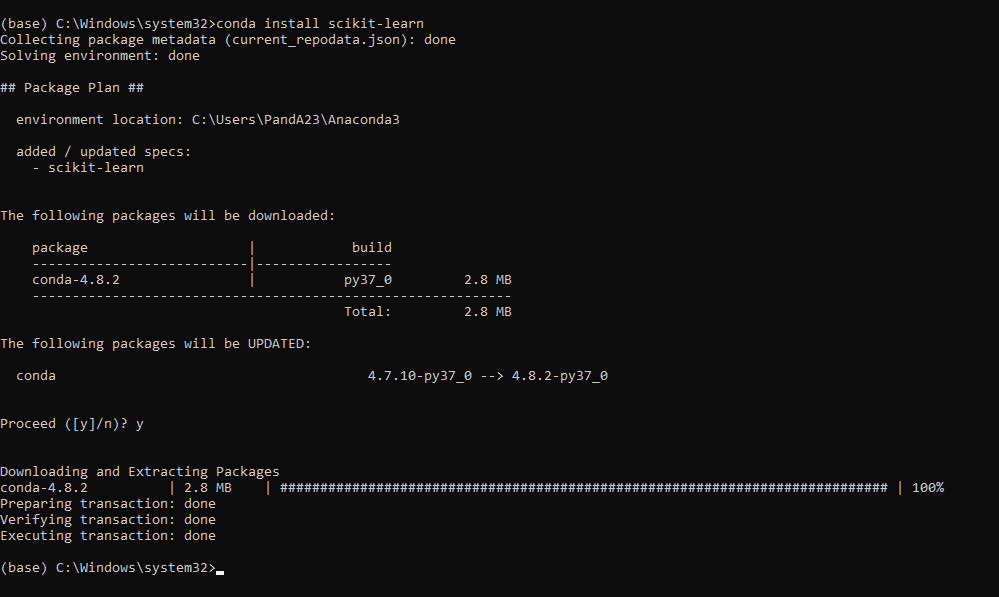
\includegraphics[width=4cm]{figures/1174087/1/instalasi.png}
		\centering
		\caption{Instalasi Package Scikit Learn}
	\end{figure}
	\begin{figure}[H]
		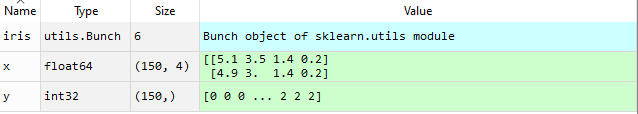
\includegraphics[width=4cm]{figures/1174087/1/variable.png}
		\centering
		\caption{Isi Variabel Explorer}
	\end{figure}
	\item Mencoba loading an example dataset
	\hfill\break
	\lstinputlisting[firstline=8, lastline=12]{src/1174087/1/1174087.py}
	\item Mencoba Learning dan predicting
	\hfill\break
	\lstinputlisting[firstline=14, lastline=24]{src/1174087/1/1174087.py}
	\item Mencoba Model Persistence
	\hfill\break
	\lstinputlisting[firstline=26, lastline=36]{src/1174087/1/1174087.py}
	\item Mencoba Conventions
	\hfill\break
	\lstinputlisting[firstline=38, lastline=50]{src/1174087/1/1174087.py}
\end{enumerate}

\subsection{Penanganan Error}
\begin{enumerate}
	\item ScreenShoot Error
	\begin{figure}[H]
		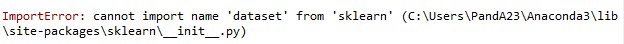
\includegraphics[width=4cm]{figures/1174087/1/import.png}
		\centering
		\caption{Import Error}
	\end{figure}
	
	\item Tuliskan Kode Error dan Jenis Error
	\begin{itemize}
		\item Import Error
	\end{itemize}
	\item Cara Penangan Error
	\begin{itemize}
		\item Import Error
		\hfill\break
		Dengan Menginstall Library Yang Tidak Ditemukan atau Memperperbaiki Penulisan Library 
	
	\end{itemize}
\end{enumerate}

\subsection{Bukti Tidak Plagiat}
\begin{figure}[H]
	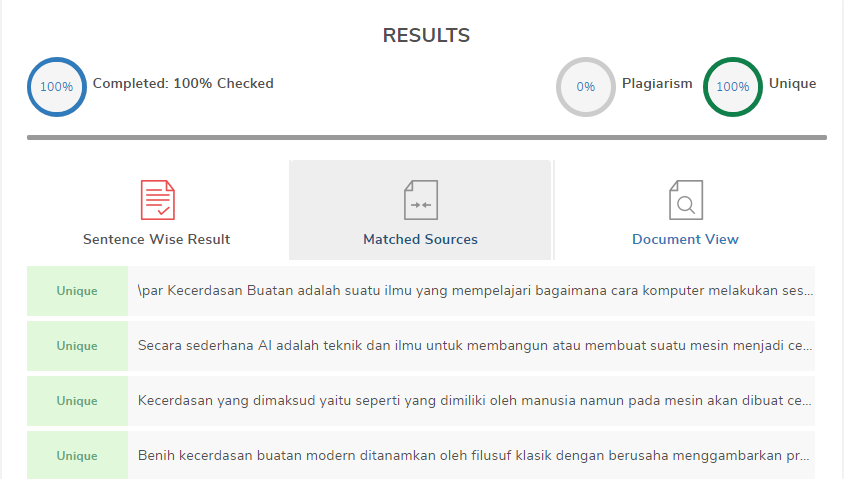
\includegraphics[width=4cm]{figures/1174087/1/plagiat.png}
	\centering
	\caption{Bukti Tidak Melakukan Plagiat}
\end{figure}

\subsection{Link Youtube:}
https://www.youtube.com/watch?v=-qw8q7jhEmg
%\section{1174084 - Muhammad Reza Syachrani}
\subsection{Teori}
\begin{enumerate}
	\item Definisi Sejarah dan Perkembangan Kecerdasan Buatan
	\hfill\break
	Definisi Kecerdasan Buatan, Kecerdasan Buatan biasa disebut dengan istilah AI (Artificial Intelligence). AI merupakan tentang bagaimana cara untuk melengkapi sebuah komputer dengan kemampuan yang dimiliki oleh manusia. Dengan demikian, Diharapkan komputer mampu mengambil keputusan sendiri untuk berbagai kasus yang ditemuinya kemudian itulah yang disebut dengan kecerdasan buatan.  Kecerdasan buatan adalah kemampuan komputer yang dikendalikan konputer untuk melakukan tugas yang umumnya dikaitkan dengan sesuatu yang cerdas.
	\hfill\break
	Sejarah Kecerdasan Buatan, Kecerdasan buatan / Artificial intelligence mulai terbentuk pada tahun 1940 dan 1950. Pada awal 50-an, studi tentang “mesin berpikir” memiliki berbagai nama seperti cybernetics, teori automata, dan pemrosesan innformasi. Pada tahun 1956, para ilmuan jenius seperti Alan Turing, Norbert, Wiener, Claude Shannon dan Warren McCullough telah bekerja secara independen dibidang cybernetics, matematika, algoritma dan teori jaringan. Namun, seprang ilmuan komputer dan kognitif John McCarthy adalah orang yang dating dengan ide untuk bergabung dengan upaya penelitian terpisah ini kedalam satu bidang yang akan mempelajari topic baru untuk imajinasi manusia yaitu kecerdasan buatan.
    Pada tahun 1956, McCarthy yang sama mendirikan Konferensi Dartmouth di Hanover, New Hampshire. Tujuan dari bidang penelitian yang baru dibuat adalah untuk mengembangkan mesin yang dapat mensimulasikan setiap aspek kecerdasab. Oleh karena itu Konferensi Dartmouth 1956 dianggap sebagai kelahiran Kecerdasan Buatan.
    \hfill\break
    Perkembangan Kecerdasan Buatan, perkembangan kecerdasan buatan dapat menggantikan berbagai pekerjaan manusia seperti kasir, operator telepon, pengendara truk, dan lainnya. AI Summer 1 (1956-1973) Konferensi Dartmounth diikuti oleh 17 tahun kemajuan luar biasa. Proyek penelitian yang dilakukan di MIT, universitas di Edinburgh, Stanford dan Carnegie Mellon menerima dana besar-besaran, yang akhirnya membuahkan hasil. Selama tahun-tahun itulah komputer pemrograman mulai melakukan masalah aljabar, membuktikan teorema geometris, memahami dan menggunakan sintaks dan tata bahasa Inggris. Terlepas dari ditinggalkannya koneksionisme dan terjemahan mesin yang gagal, yang menunda penelitian Natural Language Processing (NLP) selama bertahun-tahun, banyak prestasi dari masa lalu yang membuat sejarah. Berikut ini beberapa diantaranya : Pelopor pembelajaran mesin, Ray Solomonoff dasar-dasar teori metematika AI, memperkenalkan metode Bayesian universal untuk inferensi dan preddiksi induktif Thomas Evans menciptakan program ANALOGI heuristik, yang memungkinkan komputer memecahkan masalah geometrianalogi Unimation, perusahaan robotika pertma didunia, menciptakan robot industri Unimate, yang bekerja pada jalur perakitan modil Genenral Motors. Joseph Weizenbaum membangun ELIZA-program interaktif yang dapat membawa percakapan dalam bahasan Inggris tentang topik apapun. Ross Quillian menunjukkan jaring semanik, sedangkan Jaime Carbonell (Sr.) mengembangkan Cendikia-program interaktif untuk instruksi yang dibantu komputer berdasarkan jaring semantik. Edward Feigenbaum dan Julian Feldman menerbitkan Computeks and Thought, kumpulan artikel pertama tentang AI.
	\item Definisi Supervised learning, klasifikasi, regresi, unsupervised learning, dataset, training set dan testing set.
	\hfill\break
	\begin{itemize}
		\item Supervised Learning
		\hfill\break
		Supervised Learning merupakan tugas pengumpulan data untuk menyimpulkan fungsi dari data pelatihan berlabel. Data pelatihan terdiri dari serangkaian contoh pelatihan. Dalam supervised learning, setiap contoh adalah pasangan yang terdiri dari objek input (biasanya vektor) dan nilai output yang diinginkan(juga disebut sinyal pengawasan super).
		\item Klasifikasi
		\hfill\break
		Klasifikasi adalah pembagian sesuatu menurut kelas-kelas.  Klasifikasi merupakan proses dari pengelompokkan benda berdasarkan ciri-ciri persamaan dan juga perbedaan. Dalam masalah klasifikasi, kami mencoba memprediksi sejumlah nilai terpisah.
		\item Regresi
		\hfill\break
		Regresi adalah metode analisis statistik yang digunakan untuk melihat pengaruh antara dua ataupun lebih variabel. Regresi adalah membahas masalah ketika variabel output adalah nilai riil atau berkelanjutan, seperti ”gaji” atau ”berat”.
		\item Unsupervised learning 
		\hfill\break
		Unsupervised Learning adalah pelatihan algoritma kecerdasan buatan (AI) menggunakan informasi yang tidak diklasifikasikan atau diberi label dan memungkinkan algoritma untuk bertindak atas informasi tersebut tanpa bimbingan. Dalam Unsupervised Learning, sistem AI dapat mengelompokkan informasi yang tidak disortir berdasarkan persamaan dan perbedaan meskipun tidak ada kategori yang disediakan.
		\item Data set
		\hfill\break
		Data set objek yang merepresentasikan data dan relasinya di memory. Strukturnya mirip dengan data di database. Dataset berisi koleksi dari datatable dan datarelation.
		\item Training Set
		\hfill\break
		Training Set adalah set digunakan oleh algoritma klassifikasi. Dapat dicontohkan dengan decision tree, bayesian, neural network dll. Semuanya dapat digunakan untuk membentuk sebuah model classifier
		\item Testing Set
		\hfill\break
		Testing Set merupakan set yang digunakan untuk mengukur sejauh mana classifier berhasil melakukan klasifikasi dengan benar. Dapat berfungsi sebagai meterai persetujuan, dan Anda tidak menggunakannya sampai akhir.
	\end{itemize}
\end{enumerate}
\subsection{Praktek}
\begin{enumerate}
	\item Instalasi Library scikit dari ianaconda, mencoba kompilasi dan uji coba ambil contoh kode dan lihat variabel explorer
	\hfill\break
	\begin{figure}[H]
		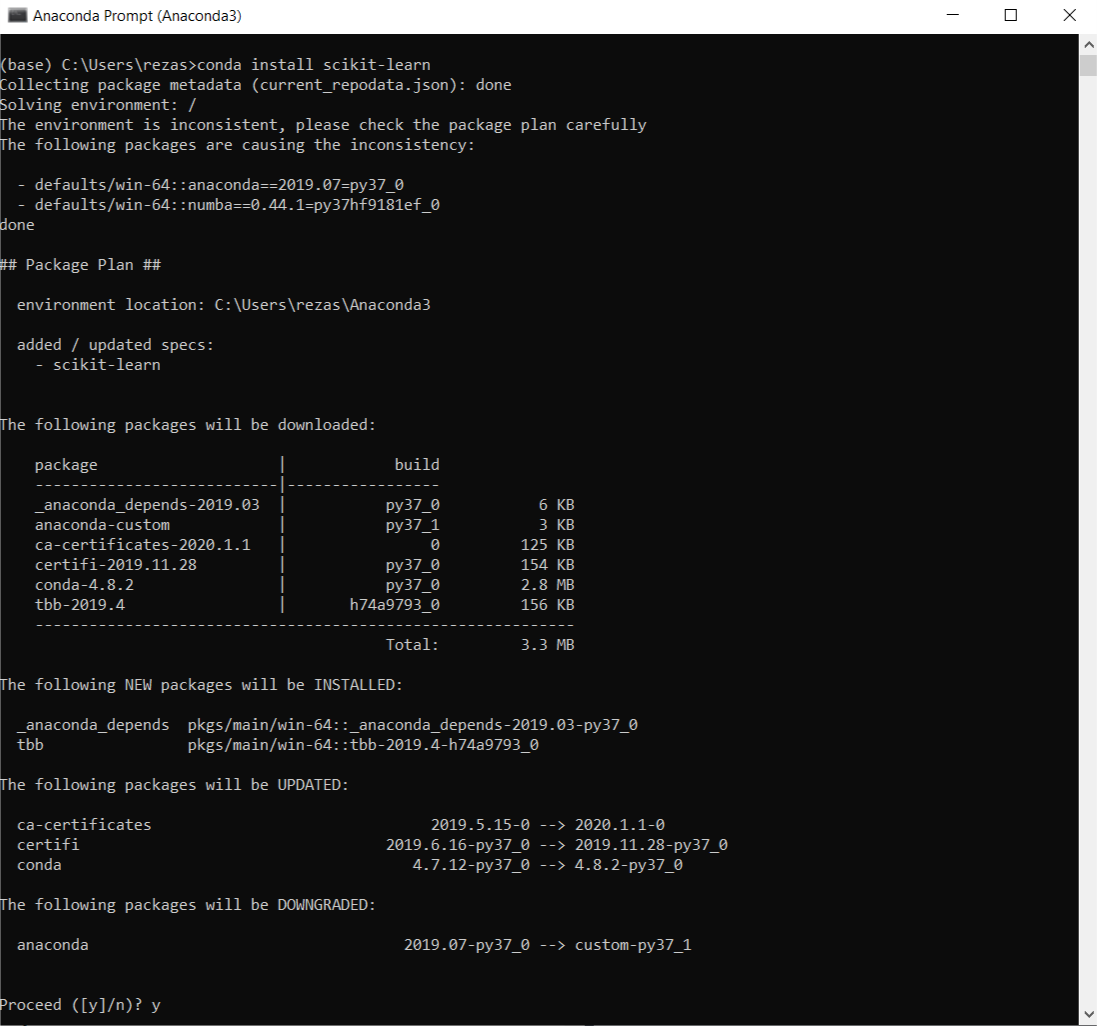
\includegraphics[width=4cm]{figures/1174084/1/1.png}
		\centering
		\caption{Instalasi Package Scikit Learn}
	\end{figure}
	\begin{figure}[H]
		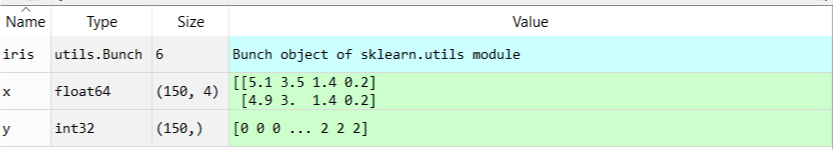
\includegraphics[width=4cm]{figures/1174084/1/2.png}
		\centering
		\caption{Isi Variabel Explorer}
	\end{figure}
	\item Mencoba loading an example dataset
	\hfill\break
	\lstinputlisting[firstline=7, lastline=11]{src/1174084/1/1174084.py}
	\item Mencoba Learning dan predicting
	\hfill\break
	\lstinputlisting[firstline=12, lastline=22]{src/1174084/1/1174084.py}
	\item Mencoba Model Persistence
	\hfill\break
	\lstinputlisting[firstline=23, lastline=33]{src/1174084/1/1174084.py}
	\item Mencoba Conventions
	\hfill\break
	\lstinputlisting[firstline=34, lastline=46]{src/1174084/1/1174084.py}
\end{enumerate}
\subsection{Penanganan Error}
\begin{enumerate}
	\item ScreenShoot Error
	\begin{figure}[H]
		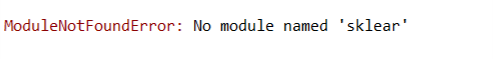
\includegraphics[width=4cm]{figures/1174084/1/error/1.png}
		\centering
		\caption{Module Error}
	\end{figure}
	\item Tuliskan Kode Error dan Jenis Error
	\begin{itemize}
		\item Module Error
	\end{itemize}
	\item Cara Penangan Error
	\begin{itemize}
		\item Module Error
		\hfill\break
		Dengan memperbaiki penulisan atau kesalahan dalam kode atau melakukan install package atau modul yang belum terinstal 
	\end{itemize}
\end{enumerate}
\subsection{Bukti Tidak Plagiat}
\begin{figure}[H]
	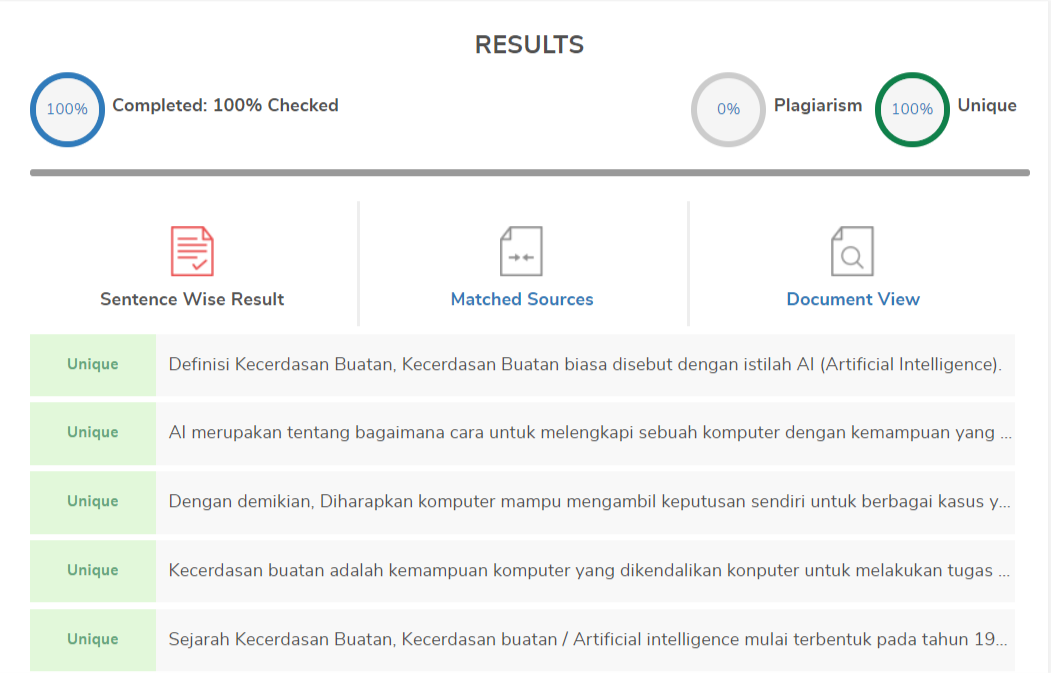
\includegraphics[width=4cm]{figures/1174084/1/plagiarisme.png}
	\centering
	\caption{Bukti Tidak Melakukan Plagiat}
\end{figure}
%\section{1174083 - Bakti Qilan Mufid}
\subsection{Teori}
\subsubsection{Kecerdasan Buatan}
\begin{enumerate}
    \item {Definisi Kecerdasan Buatan}
    \par Kecerdasan Buatan biasa disebut dengan istilah AI (Artificial Intelligence). AI sendiri merupakan suatu cabang dalam bisnis sains komputer sains dimana mengkaji tentang bagaimana cara untuk menlengkapi sebuah komputer dengan kemampuan atau kepintaran layaknya atau mirip dengan yang dimiliki manusia. Sebagai contoh, sebagaimana komputer dapat berkomunikasi dengan pengguna baik menggunakan kata, suara maupun lain sebagainya. Dengan kemampuan ini, diharapkan komputer mampu mengambil keputusan sendiri untuk berbagai kasus yang ditemuinya kemudian itulah yang disebut dengan kecerdasan buatan. Kecerdasan buatan adalah kemampuan komputer digital atau robot yang dikendalikan konputer untuk melakukan tugas yang umumnya dikaitkan dengan sesuatu yang cerdas. Istilah ini sering diterapkan pada proyek pengembangan sistem yang diberkahi dengan karakteristik proses intelektual manusia, seperti kemampuan untuk berpikir, menemukan makna, menggeneralisasi, atau belajar dari pengalaman masa lalu.

    Kecerdasan Buatan adalah salah satu bidang studi yang berhubungan dengan pemanfaatan mesin untuk memecahkan persoalan yang rumit dengan cara lebih manusiawi dan lebih bisa di pahami oleh manusia. Kecerdasan buatan makin canggih dengan kemampuan komputer dalam memperbarui pengetahuannya dengan banyaknya testing dan perkembangan target analisa. Untuk kecerdasan buatan ada banyak contoh dan jenisnya. Salah satu contoh yang paling terkenal dari Artificial Intelligence ialah Google Assistant. Google Assistant digunakan untuk kemudahan user dalam menemukan berbagai hal maupun penyetingan langsung terhadap smartphone yang digunakan dan masih banyak lagi.
    
    \item {Sejarah Kecerdasan Buatan}
    \par Artificial intelligence merupakan inovasi baru di bidang ilmu pengetahuan. Mulai terbentuk sejak adanya komputer modern dan kira-kira terjadi sekitaran tahun 1940 dan 1950. Ilmu pengetahuan komputer ini khusus ditujukan dalam perancangan otomatisasi tingkah laku cerdas dalam sistem kecerdasan komputer. Pada awal 50-an, studi tentang “mesin berpikir” memiliki berbagai nama seperti cybernetics, teori automata, dan pemrosesan innformasi. Pada tahun 1956, para ilmuan jenius seperti Alan Turing, Norbert, Wiener, Claude Shannon dan Warren McCullough telah bekerja secara independen dibidang cybernetics, matematika, algoritma dan teori jaringan. Namun, seprang ilmuan komputer dan kognitif John McCarthy adalah orang yang dating dengan ide untuk bergabung dengan upaya penelitian terpisah ini kedalam satu bidang yang akan mempelajari topic baru untuk imajinasi manusia yaitu kecerdasan buatan. Dia adalah orang yang menciptakan istilah tersebut dan kemudian mendirikan laboratorium Kecerdasan Buatan di MIT dan Stan ford.

    Pada tahun 1956, McCarthy yang sama mendirikan Konferensi Dartmouth di Hanover, New Hampshire. Peneliti terkemuka dalam teori kompleksitas, simulasi bahasa, hubungan antara keacakan dan pemikiran kreatif, jaringan saraf diundang. Tujuan dari bidang penelitian yang baru dibuat adalah untuk mengembangkan mesin yang dapat mensimulasikan setiap aspek kecerdasab. Itulah sebabnya Konferensi Dartmouth 1956 dianggap sebagai kelahiran Kecerdasan Buatan. Sejak saat itu, Kecerdasa Buatan telah hidup melalui decade kemuliaan dan cemoohan, yang dikenal luas sebagai musim panas dan musim dingin AI. Musim panasnya ditandai dengan optimism dan dana besar, sedangkan musim dinginnya dihadapkan dengan pemotongan dana, ketidakkpercayaan dan pesimisme.

    \item{Perkembangan Kecerdasan Buatan}
    \par Teknologi Artificial Intelligence semakin ramai dibahas dalam berbagai diskusi teknologi di seluruh dunia.Menurut kebanyakan orang, pekerjaan seperti kasir, operator telepon, pengendara truk, dan lainnya sangat berpeluang besar untuk tergantikan oleh Artificial Intelligence. Mengapa terjadi hal demikian? dikarenakan memang bahwa AI lebih ungul dalam hal kinerja, fitur dan lain sebagainya. Namun, dalam beberapa aspek memang pekerja manusia masih unggul dibandingkan AI itu sendiri. Para generasi muda yang ada di dunia terutama di daerah Asia terlihat sudah memahami fungsi dan efek dari AI dalam kehidupan kita sehari-hari. Berdasarkan survei yang dilakukan oleh Microsoft, terdapat 39 persen responden yang mempertimbangkan untuk menggunakan mobil tanpa pengemudi dan 36 persen lainnya setuju bahwa robot masa depan dengan software untuk beroperasi mampu meningkatkan produktivitas. Dari survey tersebut kita sebagai pengguna AI harus lebih bijaksana dalam pengembangan dan penggunaan dari AI sehingga tanpa memberikan efek samping terhadap etos kerja dan keseharian kita sebagai pengguna dalam kehidupan sehari-hari.

    AI Summer 1 (1956-1973) KOnferensi Dartmounth diikuti oleh 17 tahun kemajuan luar biasa. Proyek penelitian yang dilakukan di MIT, universitas di Edinburgh, Stanford dan Carnegie Mellon menerima dana besar-besaran, yang akhirnya membuahkan hasil. Selama tahun-tahun itulah komputer pemrograman mulai melakukan masalah aljabar, membuktikan teorema geometris, memahami dan menggunakan sintaks dan tata bahasa Inggris. Terlepas dari ditinggalkannya koneksionisme dan terjemahan mesin yang gagal, yang menunda penelitian Natural Language Processing (NLP) selama bertahun-tahun, banyak prestasi dari masa lalu yang membuat sejarah. Berikut ini beberapa diantaranya : Pelopor pembelajaran mesin, Ray Solomonoff meletakkan dasar-dasar teori metematika AI, memperkenalkan metode Bayesian universal untuk inferensi dan preddiksi induktif Thomas Evans menciptakan program ANALOGI heuristik, yang memungkinkan komputer memecahkan masalah geometri-analogi Unimation, perusahaan robotika pertma didunia, menciptakan robot industri Unimate, yang bekerja pada jalur perakitan modil Genenral Motors. Joseph Weizenbaum membangun ELIZA-program interaktif yang dapat membawa percakapan dalam bahasan Inggris tentang topik apapun. Ross Quillian menunjukkan jaring semanik, sedangkan Jaime Carbonell (Sr.) mengembangkan Cendikia-program interaktif untuk instruksi yang dibantu komputer berdasarkan jaring semantik. Edward Feigenbaum dan Julian Feldman menerbitkan Computeks and Thought, kumpulan artikel pertama tentang AI.

\end{enumerate}

\subsubsection{Scikit-Learn}
\begin{enumerate}
    \item{Supervised Learning}
    \par Supervised Learning adalah tugas pengumpulan data untuk menyimpulkan fungsi dari data pelatihan berlabel. Data pelatihan terdiri dari serangkaian contoh pelatihan. Dalam supervised learning, setiap contoh adalah pasangan yang terdiri dari objek input (biasanya vektor) dan nilai output yang diinginkan(juga disebut sinyal pengawasan super). Algoritma pembelajaran yang diawasi menganalisis data pelatihan dan menghasilkan fungsi yang disimpulkan, yang dapat digunakan untuk memetakan contoh-contoh baru. Skenario optimal akan memungkinkan algoritma menentukan label kelas dengan benar untuk instance yang tidak terlihat. Ini membutuhkan algoritma pembelajaran untuk menggeneralisasi dari data pelatihan untuk situasi yang tidak terlihat dengan cara yang "masuk akal". Supervised Learning adalah pendekatan dimana sudah terdapat data yang dilatih selain itu juga terdapat variable yang ditargetkan sehingga tujuan dari pendekatan ini yaitu mengelompokkan suatu data ke dta yang sudah ada. Supervised Learning menyediakan algoritma pembelajaran dengan jumlah yang diketahui untuk mendukung penilaian dimasa depan. Chatbots, mobil self-driving, program pengenalan wajah, sistem pakar dan robot adalah beberapa sistem yang dapat menggunakan pembelajaran yang diawasi atau tidak diawasi. Supervised Learning sebagian besar terkait dengan AI berbasis pengambilan tetapi mereka juga mungkin mampu menggunakan model pembelajaran generatif. Data pelatihan untuk pembelajaran yang diawasi mencakup serangkaian contoh dengan subjek input berpasangan dan output yang diinginkan (yang juga disebut sebagai sinyal pengawasan).

    Dalam pembelajaran yang diawasi untuk pemrosesan gambar, misalnya sistem AI mungkin dilengkapi dengan gambar berlabel kendaraan dalam ketegori seperti mobil dan truk. Setelah jumlah pengamatan yang cukup, sistem harus dapat membedakan antara dan mengkategorikan gambar yang tidak berlabel, dimana waktu pelatihan dapat dikatakan lengkap. Model Supervised Learning memiliki beberapa keunggulan dibandingkan pendekatan tanpa pengawasan, tetapi mereka juga memiliki keterbatasan. Sistem lebih cenderung membuat penilaian bahwa manusia dapat berhubungan, misalnya karena manusia telah memberikan dasar untuk keputusan. Namun, dalam kasus metode berbasis pengambilan, Supervised Learning mengalami kesulitan dalam menangani informaasi baru. Jika suatu sistem dengan kategori untuk mobil dan truk disajikan dengan sepeda, misalnya ia harus salah dikelompokkan dalam satu kategori ata yang lain. Namun. jika sistem AI bersifat generatif, ia mungkin tidak tahu apa sepeda itu tetapi akan dapat mengenalinya sebagai milik kategori yang terpisah.

    \item{Regresi}
    \par Regresi adalah metode analisis statistik yang digunakan untuk melihat pengaruh antara dua ataupun lebih variabel. Regresi adalah membahas masalah ketika variabel output adalah nilai riil atau berkelanjutan, seperti "gaji" atau "berat". Banyak model yang berbeda dapat digunakan makan, yang paling sederhana adalah regresi linier. Ia mencoba untuk menyesuaikan data dengan hyper-plane terbaik yang melewati poin.

    \item{Klasifikasi}
    \par Klasifikasi adalah pembagian sesuatu menurut kelas-kelas ( class ). Menurut Ilmu Pengetahuan, Klasifikasi merupakan proses pengelompokkan benda berdasarkan ciri-ciri persamaan dan juga perbedaan. Dalam masalah klasifikasi, kami mencoba memprediksi sejumlah nilai terpisah. Label (y) umumnya datang dalam bentuk kategorikal dan mewakili sejumlah kelas. Dalam pembelajaran mesin dan statistik, klasifikasi adalah pendekatan pembelajaran yang diawasi di mana program komputer belajar dari input data yang diberikan kepadanya dan kemudian menggunakan pembelajaran ini untuk mengklasifikasikan pengamatan baru. Kumpulan data ini mungkin hanya bersifat dua kelas (seperti mengidentifikasi apakah orang tersebut berjenis kelamin laki-laki atau perempuan atau bahwa surat itu spam atau bukan-spam) atau mungkin juga multi-kelas. Beberapa contoh masalah klasifikasi adalah: pengenalan ucapan, pengenalan tulisan tangan, identifikasi metrik, klasifikasi dokumen dll.

    \item{Unsupervised Learning}
    \par Unsupervised Learning berbeda dengan Supervised Leraning. Perbedaannya ialah unsupervised learning tidak memiliki data latih, sehingga dari data yang ada kita mengelompokan data tersebut menjadi 2 ataupun 3 bagian dan seterusnya. Unsupervised Learning adalah pelatihan algoritma kecerdasan buatan (AI) menggunakan informasi yang tidak diklasifikasikan atau diberi label dan memungkinkan algoritma untuk bertindak atas informasi tersebut tanpa bimbingan. Dalam Unsupervised Learning, sistem AI dapat mengelompokkan informasi yang tidak disortir berdasarkan persamaan dan perbedaan meskipun tidak ada kategori yang disediakan.

    Dalam Unsupervised Learning, sistem AI disajikan dengan data yang tidak berlabel, tidak terkategorisasi dan algoritma sistem bekerja pada data tanpa pelatihan sebelumnya. Outputnya tergantung pada algoritma kode. Menundukkan suatu sistem pada Unsupervised Learning adalah salah satu cara untuk menguji AI. Algoritma Unsupervised Learning dapat melakukan tugas pemrosesan yang lebih kompleks daripada sistem pembelajaran yang diawasi. Namun, pembelajaran tanpa pengawasan bisa lebih tidak terduga daripada model alternatif. Sementara Unsupervised Learningi mungkin, misalnya, mencari tahu sendiri cara memilah kucing dari anjing, mungkin juga menambahkan kategori yang tidak terduga dan tidak diinginkan untuk menangani breed yang tidak biasa, membuat kekacauan bukannya keteraturan

    \item{Data Set}
    \par Dataset adalah objek yang merepresentasikan data dan juga relasi yang ada di memory. Strukturnya mirip dengan data di database, namun bedanya dataset berisi koleksi dari data table dan data relation. mendapatkan data yang tepat berarti mengumpulkan atau mengidentifikasi data yang berkorelasi dengan hasil yang ingin Anda prediksi; yaitu data yang berisi sinyal tentang peristiwa yang Anda pedulikan. Data harus diselaraskan dengan masalah yang Anda coba selesaikan. Gambar kucing tidak terlalu berguna ketika Anda sedang membangun sistem identifikasi wajah. Memverifikasi bahwa data selaras dengan masalah yang ingin Anda selesaikan harus dilakukan oleh ilmuwan data. Jika Anda tidak memiliki data yang tepat, maka upaya Anda untuk membangun solusi AI harus kembali ke tahap pengumpulan data. Format ujung kanan untuk pembelajaran dalam umumnya adalah tensor, atau array multi-dimensi. Jadi jalur pipa data yang dibangun untuk pembelajaran mendalam umumnya akan mengkonversi semua data - baik itu gambar, video, suara, suara, teks atau deret waktu  menjadi vektor dan tensor yang dapat diterapkan operasi aljabar linier. Data itu seringkali perlu dinormalisasi, distandarisasi dan dibersihkan untuk meningkatkan kegunaannya, dan itu semua adalah langkah dalam ETL pembelajaran mesin. Deeplearning4j menawarkan alat ETV DataVec untuk melakukan tugas-tugas pemrosesan data tersebut.

    Pembelajaran yang dalam, dan pembelajaran mesin yang lebih umum, membutuhkan pelatihan yang baik agar bekerja dengan baik. Mengumpulkan dan membangun set pelatihan  badan yang cukup besar dari data yang diketahui  membutuhkan waktu dan pengetahuan khusus domain tentang di mana dan bagaimana mengumpulkan informasi yang relevan. Perangkat pelatihan bertindak sebagai tolok ukur terhadap mana jaring pembelajaran dalam dilatih. Itulah yang mereka pelajari untuk direkonstruksi sebelum mereka melepaskan data yang belum pernah mereka lihat sebelumnya. Pada tahap ini, manusia yang berpengetahuan luas perlu menemukan data mentah yang tepat dan mengubahnya menjadi representasi numerik yang dapat dipahami oleh algoritma pembelajaran mendalam, tensor. Membangun set pelatihan, dalam arti tertentu, pra-pra pelatihan. Set pelatihan yang membutuhkan banyak waktu atau keahlian dapat berfungsi sebagai keunggulan dalam dunia ilmu data dan pemecahan masalah. Sifat keahlian sebagian besar dalam memberi tahu algoritma Anda apa yang penting bagi Anda dengan memilih apa yang masuk ke dalam set pelatihan. Ini melibatkan menceritakan sebuah kisah  melalui data awal yang Anda pilih yang akan memandu jaring pembelajaran mendalam Anda saat mereka mengekstraksi fitur-fitur penting, baik di set pelatihan maupun dalam data mentah yang telah mereka ciptakan untuk dipelajari. Untuk membuat set pelatihan yang bermanfaat, Anda harus memahami masalah yang Anda selesaikan; yaitu apa yang Anda inginkan agar jaring pembelajaran mendalam Anda memperhatikan, di mana hasil yang ingin Anda prediksi.

    \item{Training Set}
    \par Training Set adalah set digunakan oleh algoritma klassifikasi . Dapat dicontohkan dengan : decision tree, bayesian, neural network dll. Semuanya dapat digunakan untuk membentuk sebuah model classifier. Menjalankan pelatihan yang diatur melalui jaringan saraf mengajarkan pada net cara menimbang berbagai fitur, menyesuaikan koefisien berdasarkan kemungkinan mereka meminimalkan kesalahan dalam hasil Anda. Koefisien-koefisien tersebut, juga dikenal sebagai parameter, akan terkandung dalam tensor dan bersama-sama mereka disebut model, karena mereka mengkodekan model data yang mereka latih. Mereka adalah takeaways paling penting yang akan Anda dapatkan dari pelatihan jaringan saraf.

    \item{Testing Set}
    \par Testing Set adalah set yang digunakan untuk mengukur sejauh mana classifier berhasil melakukan klasifikasi dengan benar. Ini berfungsi sebagai meterai persetujuan, dan Anda tidak menggunakannya sampai akhir. Setelah Anda melatih dan mengoptimalkan data Anda, Anda menguji jaringan saraf Anda terhadap pengambilan sampel acak akhir ini. Hasil yang dihasilkannya harus memvalidasi bahwa jaring Anda secara akurat mengenali gambar, atau mengenalinya setidaknya [x] dari jumlah tersebut. Jika Anda tidak mendapatkan prediksi yang akurat, kembalilah ke set pelatihan, lihat hyperparameter yang Anda gunakan untuk menyetel jaringan, serta kualitas data Anda dan lihat teknik pra-pemrosesan Anda.
\end{enumerate}


\subsection{Praktek}
\subsubsection{Instalasi library scikit dari anaconda, mencoba kompilasi dan uji coba ambil contoh kode dan lihat variabel explorer}
\begin{enumerate}
\item Pastikan anda telah menginstall anaconda lalu buka aplikasi Anaconda Prompt

\item Lalu pastikan anda telah menginstall python

\item Pada Anaconda Prompt install scikit dengan cara conda install scikit-learn
\begin{figure}[H]
	\begin{center}
   	 \includegraphics[width=10cm]{figures/1174083/figures1/1.jpg}
   	 \caption{Instalasi Scikit Dari Anaconda Prompt}	
	\end{center}
\end{figure}

\item Lalu tulis kode yang ada dibawah ini dan run menggunakan spyder
\lstinputlisting[firstline=1, lastline=4]{src/1174083/src1/coba.py}
\begin{figure}[H]
	\begin{center}
   	 \includegraphics[width=10cm]{figures/1174083/figures1/2.jpg}
   	 \caption{Running Kode dari Spyder dan Hasil Variable Explorer}	
	\end{center}
\end{figure}
\end{enumerate}

\subsubsection{Loading an example dataset}
\begin{figure}[H]
	\begin{center}
   	 \includegraphics[width=10cm]{figures/1174083/figures1/3.jpg}
   	 \caption{Running Loading an example dataset dari Spyder}	
	\end{center}
\end{figure}

\begin{itemize}
\item Import fungsi datasets dari library sklearn
\lstinputlisting[firstline=1, lastline=1]{src/1174083/src1/coba.py}

\item Memasukkan data dari datasets iris ke variable iris
\lstinputlisting[firstline=2, lastline=2]{src/1174083/src1/coba.py}

\item Memasukkan data dari datasets digits ke variable digits
\lstinputlisting[firstline=3, lastline=3]{src/1174083/src1/coba.py}

\item Menampilkan data dari datasets digits ke console
\lstinputlisting[firstline=4, lastline=4]{src/1174083/src1/coba.py}
\begin{figure}[H]
	\begin{center}
   	 \includegraphics[width=10cm]{figures/1174083/figures1/5.jpg}
   	 \caption{Hasil Running kode loading an example dataset}	
	\end{center}
\end{figure}
\end{itemize}

\subsubsection{Learning and predicting}
\begin{itemize}
\item Buka Anaconda Prompt
\begin{figure}[H]
	\begin{center}
   	 \includegraphics[width=10cm]{figures/1174083/figures1/anaconda.jpg}
   	 \caption{Anaconda Prompt}	
	\end{center}
\end{figure}

\item Lalu kita import datasets dari sklearn seperti dibawah ini
\begin{figure}[H]
	\begin{center}
   	 \includegraphics[width=10cm]{figures/1174083/figures1/5.jpg}
   	 \caption{Menggunakan datasets}	
	\end{center}
\end{figure}

\item lalu kita mendefisisikan iris dan digits menjadi variable
\begin{figure}[H]
	\begin{center}
   	 \includegraphics[width=10cm]{figures/1174083/figures1/6.jpg}
   	 \caption{mendefinisikan iris}	
	\end{center}
\end{figure}
\begin{figure}[H]
	\begin{center}
   	 \includegraphics[width=10cm]{figures/1174083/figures1/7.jpg}
   	 \caption{mendefinisikan digits}	
	\end{center}
\end{figure}

\item Lalu kita import svm dari sklearn yang nantinya digunakan untuk menjadi estimanasi angka kita
\begin{figure}[H]
	\begin{center}
   	 \includegraphics[width=10cm]{figures/1174083/figures1/4.jpg}
   	 \caption{Menggunakan svm}	
	\end{center}
\end{figure}

\item Lalu, kita definisikan clf sebagai classfier, disini gamma didefinisikan secara manual
\begin{figure}[H]
	\begin{center}
   	 \includegraphics[width=10cm]{figures/1174083/figures1/8.jpg}
   	 \caption{Mendefinisikan Classifier}	
	\end{center}
\end{figure}

\item Estimator clf (for classifier) pertama kali dipasang pada model. Ini dilakukan dengan melewati training set ke metode fit. Untuk training set, akan menggunakan semua gambar dari set data yang ada, kecuali untuk gambar terakhir, yang dicadangan untuk prediksi. Pada skrip dibawah memilih training set dengan sintaks Python [: -1], yang menghasilkan array baru yang berisi semua kecuali item terakhir dari digits.
\begin{figure}[H]
	\begin{center}
   	 \includegraphics[width=10cm]{figures/1174083/figures1/9.jpg}
   	 \caption{Memanggil Classifier}	
	\end{center}
\end{figure}

\item Menunnjukkan prediksi angka baru
\begin{figure}[H]
	\begin{center}
   	 \includegraphics[width=10cm]{figures/1174083/figures1/10.jpg}
   	 \caption{Prediksi nilai baru}	
	\end{center}
\end{figure}
\end{itemize}
\lstinputlisting[firstline=8 lastline=15]{src/1174083/src1/coba2.py}

\subsubsection{Model Persistance}
Model Persistance
\lstinputlisting[firstline=8 lastline=32]{src/1174083/src1/coba3.py}


\subsubsection{Conventions}
Conversion
\lstinputlisting[firstline=8 lastline=19]{src/1174083/src1/coba4.py}

\subsection{Penanganan Error}

Dari percobaan yang dilakukan di atas, apabila mendapatkan error maka:
\begin{enumerate}

\item Screenshoot Error
\begin{figure}[H]
	\begin{center}
   	 \includegraphics[width=10cm]{figures/1174083/figures1/error1.jpg}
   	 \caption{ImportError: cannot import name 'datasetss' from 'sklearn'}	
	\end{center}
\end{figure}
	
\item Tuliskan kode eror dan jenis errornya [hari ke 2](10)
\begin{itemize}
\item ImportError
\end{itemize}

\item Solusi pemecahan masalah error tersebut[hari ke 2](10)
\begin{itemize}
\item ImportError

Cek kembali jika ada yang typo
\end{itemize}

\end{enumerate}

\subsection{Bukti Tidak Plagiat}
\begin{figure}[H]
	\includegraphics[width=4cm]{figures/1174083/figures1/plagiat.jpg}
	\centering
	\caption{Bukti Tidak Melakukan Plagiat Chapter 1}
\end{figure}

\subsection{Link Youtube}
https://youtu.be/w4lTVoumb1g

%\section{Sekar Jasmine 1174075}
\subsection{Pengertian Kecerdasan Buatan}
kecerdasan buatan adalah salah satu cabang ilmu pengetahuan yang berhubungan dengan mesin untuk memecahkan persoalan yang rumit dengan cara yang lebih manusiawi. Hal ini biasanya dilakukan dengan mengikuti karakteristik dan anologi berpikir dari kecerdasan  atau inteligance manusia, dan menerapkan sebagai algoritma yang dikenal oleh komputer.
Dengan suatu pendekatan yang kurang lebih fleksibilitas dan efisien dapat diambil tergantung keperluan yang mempengaruhi bagaimana wujud dari prilaku kecerdasan buatan. AI biasanya dihubungkan dengan ilmu komputer, akan tetapi juga terkait erat dengan bidang lain seperti matematika, Psikologi, Pengamatan, Biolog, filosofi, dan lainnya
\subsection{Sejarah Kecerdasan Buatan}
Kecerdasan buatan merupakan bidang ilmu komputer yang sangat penting di era kini dan masa yang akan datang untuk mewujudkan sistem komputer yang cerdas. Bidang ini telah berkembang sangat pesat di 20 tahun terakir seiring dengan kebutuhan perangkat cerdas pada industry dan rumah tangga.
Kata Intelligance berasal dari bahasa latin "intelligo" yang berarti "saya paham". Berarti dasar dari intelligance adalah kemampuan untuk memahami dan melakukan aksi. nyatanya, bidang Kecerdasan Buatan atau disingkat dengan AI, berawal dari kemunculan komputer sekitar tahun 1940-an, sedangkan perkembangan sejarah dapat ditelusuri sejak zaman Mesir kuno. Pada saat ini, perhatian mendesak diberikan pada kemampuan komputer untuk melakukan hal-hal yang dapat dilakukan manusia. Dalam hal ini, komputer ini dapat meningkatkan kemampuan kecerdasan dan kecerdasan manusia.
Pada awal abad ke-17, René berbicara tentang tubuh binatang yang tidak meminta apa pun selain mesin yang rumit. Blaise Pascal membuat mesin hitung digital mekanis pertama pada tahun 1642. Pada 19, Charles Babbage dan Ada Lovelace bekerja pada mesin hitung mekanis yang dapat diprogram. Bertrand Russell dan Alfred Whitehead North menerbitkan Principia Mathematica, yang merombak logistik formal. Warren McCulloch dan Walter Pitts menerbitkan "Kalkulus Logika Gagasan yang Menjaga Aktivitas" pada tahun 1943 yang membentuk dasar bagi jaringan saraf.
1950-an adalah periode upaya aktif dalam AI. program permainan catur yang ditulis oleh Dietrich Prinz. John McCarthy menciptakan istilah "kecerdasan buatan" pada konferensi pertama yang menjadi dasar perjanjian itu, pada tahun 1956. Dia juga menemukan bahasa pemrograman Lisp. Alan Turing memperkenalkan "tes Turing" sebagai cara untuk mengoperasionalkan tes kecerdasan cerdas. 
\subsection{Perkembangan dan Penggunaan Kecerdasan}
Menurut studi Harvard Business Review dan ICM Unlimited pada tahun 2016, perusahaan besar memberikan kompensasi 10 persen lebih tinggi untuk setiap karyawan, Terrelong melanjutkan pengembangan Artificial Intelligence (AI) tidak hanya untuk membuat gambar atau video palsu lebih mudah, tetapi juga membuatnya sulit untuk membuktikan materi.Meskipun pada saat ini, upaya untuk membuat dan mendistribusikan konten hoax, alias hoaks, masih dapat diatasi, tetapi berhasil, tantangan yang dihadapi semakin sulit. Selain itu, AI memungkinkan pembuatan gambar, video, atau audio palsu dari bahan yang relatif minim.Moody's, yang harus disetujui, membuktikan upaya itu akan semakin menantang dan membutuhkan teknik forensik yang lebih canggih.Pada Mei 2019, para peneliti di Samsung AI Center dan Institut Sains dan Teknologi Skolkovo di Moskow, Rusia menunjukkan bahwa mereka dapat membuat tayangan video yang menampilkan masing-masing individu. Video ini sangat realistis tetapi sebenarnya palsu, dibuat menggunakan model pembelajaran tertentu yang disebut Generative Adversarial Network (GAN).Hasil dari proses GAN disebut deepfakes karena mereka menggunakan teknik pembelajaran yang mendalam untuk membuat konten palsu.Untuk jangka pendek, perusahaan diharapkan untuk terus memainkan media sosial dan situs untuk melihat pentingnya disinformasi dan meminta mereka yang bertanggung jawab untuk media sosial dan situs terkait untuk mengunduh konten.Terrelonge menambahkan langkah lain yang bisa diambil untuk merilis materi resmi untuk melawan konten palsu."Perlawanan terhadap konten palsu membutuhkan kombinasi teknologi dan pendidikan,".
\section{resume mengenai definisi supervised learning, klarifikasi, regresi, dan un-supervised learning. Data Set, training set dan testing set}
\subsection{Sipervised Learning}Supervised Learning adalah tugas mengumpulkan data untuk melengkapi fungsi data pelatihan yang diberi label. Data pelatihan terdiri dari contoh pelatihan. Dalam pembelajaran terawasi, setiap contoh adalah pasangan yang terdiri dari objek input (biasanya vektor) dan nilai output dingin (juga disebut sinyal pengawasan super). Algoritma pembelajaran yang diawasi menganalisis data pelatihan dan menghasilkan fungsi yang lengkap, yang dapat digunakan untuk memetakan contoh-contoh baru. Skenario  akan memungkinkan algoritma menentukan lable kelas dengan benar untuk instance yang tidak terlihat. Ini membutuhkan algoritma pembelajaran untuk menggeneralisasi data pelatihan sehingga tidak muncul dengan cara yang "masuk akal". Pembelajaran terawasi semakin dekat di mana ada pelatihan praktis selain dapat bervariasi yang berarti tujuannya adalah di mana mengelompokkan data ke dalam database yang ada. Pembelajaran terawasi menyediakan jumlah pembelajaran yang direkomendasikan untuk mendukung penilaian di masa depan. Obrolan, program mengemudi mandiri, pengenalan wajah, tatap muka dan robot adalah beberapa sistem yang dapat menggunakan pembelajaran yang diawasi atau tidak diawasi. Pembelajaran terbimbing sebagian besar terkait dengan AI berdasarkan pengambilan mereka juga mungkin diperlukan menggunakan model pembelajaran generatif. Pelatihan data untuk pembelajaran dimulai dengan mendiskusikan contoh-contoh dengan subjek input berpasangan dan output yang diinginkan (juga disebut sebagai sinyal pengawasan). Dalam pembelajaran yang diawasi untuk pemrosesan gambar, misalnya sistem AI dapat lengkap dengan gambar mengemudi yang berlabel dalam kategori mobil dan truk. Setelah jumlah yang memadai, sistem harus dapat membedakan antara dan mengklasifikasikan gambar yang tidak berlabel, di mana waktu pelatihan dapat diselesaikan secara penuh. Model Pembelajaran Terpandu memiliki beberapa keunggulan dibandingkan pengawasan, tetapi mereka juga memiliki keterbatasan. Sistem lebih cenderung membuat penilaian bahwa hak asasi manusia dapat dihubungkan, misalnya karena manusia telah memberikan dasar untuk pengambilan keputusan. Namun, dalam hal metode berbasis pengambilan, Supervised Learning menghilangkan kesulitan dalam menangani informasi baru. Jika sistem dikategorikan untuk mobil dan truk, maka sepeda disediakan, misalnya, harus dikelompokkan dalam satu kategori atau yang lain. Namun. Jika sistem AI generatif, mungkin tidak tahu apa itu sepeda tetapi akan dapat mengenalinya sebagai milik kategori yang terpisah.
\subsection{Klasifikasi}
Klasifikasi adalah pembagian hal sesuai dengan kelas (kelas). Menurut Science, klasifikasi adalah proses pengelompokan materi berdasarkan karakteristik dan perbedaan yang sama. Dalam masalah klasifikasi, kami mencoba memprediksi sejumlah nilai yang terpisah. Label (y) Umumnya datang dalam bentuk kategorikal dan mewakili sejumlah kelas. Dalam pembelajaran statistik dan pembelajaran mesin statistik, klasifikasi adalah pembelajaran yang dimulai ketika sebuah program komputer belajar dari input data yang disediakan untuk mendukung dan kemudian menggunakan pembelajaran ini untuk mengklasifikasikan pembelajaran baru. Pengumpulan data ini mungkin hanya dua kelas (seperti mengidentifikasi apakah orang ini laki-laki atau perempuan atau orang itu adalah spam atau bukan-spam) atau mungkin juga multi-kelas. Beberapa contoh masalah klasifikasi adalah: pengenalan ucapan, pengenalan tulisan tangan, metrik identifikasi, klasifikasi dokumen dll.
\subsection{Regresi}
Regresi adalah metode analisis statistik yang digunakan untuk melihat perbedaan antara dua atau lebih variabel. Regresi sedang membahas masalah kompilasi, variabel output adalah nilai nyata atau dipertahankan, seperti "gaji" atau "berat". Banyak model yang berbeda dapat digunakan untuk makan, cara paling sederhana adalah linearitas linear. Itu mencoba untuk mencocokkan data dengan pesawat-hyper terbaik yang melewati titik.
\subsection{unsupervised learning}
Belajar tanpa pengawasan berbeda dari Belajar dengan Supervisi. Perbedaannya adalah bahwa pembelajaran tanpa pengawasan tidak memiliki data pelatihan, jadi dari data yang tersedia kami mengelompokkan data menjadi 2 atau 3 bagian dan seterusnya. Unsupervised Learning adalah pelatihan dalam algoritma kecerdasan buatan (AI) menggunakan informasi yang tidak diklasifikasikan atau diberi label dan menyediakan algoritma untuk memperbaiki informasi yang diberikan tanpa bimbingan. Dalam Unattended Learning, sistem AI dapat mengklasifikasikan informasi yang tidak diurutkan berdasarkan ekuitas dan perbedaan dalam kategori mendadak yang disediakan. Dalam Supervised Learning Learning, sistem AI disajikan dengan sistem wajib yang tidak diberi label, tidak dikategorikan dan algoritma bekerja pada data tanpa pelatihan sebelumnya. Outputnya tergantung pada algoritma kode. Menyerahkan sistem untuk Belajar Tanpa Pengawasan adalah salah satu cara untuk menerima AI. Algoritma Pembelajaran tanpa pengawasan dapat melakukan tugas yang lebih kompleks daripada sistem pembelajaran yang diawasi. Namun, pembelajaran tanpa pengawasan dapat lebih tidak konsisten dengan model alternatif. Sementara Supervised Learning Might, misalnya, mencari sendiri dengan memilih kucing dari anjing, ia juga dapat menambahkan kategori yang tidak diinginkan dari yang tidak diinginkan untuk ditingkatkan menjadi ras yang tidak biasa, membuat pesanan diperlukan.
\subsection{Data Set}
Dataset adalah objek yang mewakili data dan hubungan dalam memori. Strukturnya mirip dengan basis data basis data, tetapi hanya kumpulan data yang dikumpulkan dari catatan dan latar belakang yang diaktifkan. dapatkan persetujuan yang tepat untuk mengumpulkan atau mengidentifikasi data yang berkorelasi dengan hasil yang ingin Anda hasilkan; yaitu data yang berisi sinyal tentang acara yang Anda sukai. Data harus disinkronkan dengan masalah yang Anda coba selesaikan. Gambar kucing bukan kompilasi yang sangat berguna. Anda sedang membangun sistem identifikasi wajah. Memodifikasi data yang selaras dengan masalah yang ingin Anda selesaikan harus dilakukan oleh para ahli data. Jika Anda tidak memiliki data yang benar, maka upaya Anda untuk membuat solusi AI harus kembali ke instalasi data. Format ujung kanan untuk belajar secara umum adalah array tensor, atau multi-dimensional. Jadi pipa data yang dibangun untuk pembelajaran dibangun secara umum untuk mengubah semua gambar, video, suara, suara, teks atau deret waktu menjadi vektor dan tensor yang dapat digunakan operasi aljabar linier. Data yang diperlukan perlu dinormalisasi, distandarisasi dan dikembalikan untuk meningkatkan kegunaannya, dan semua ini adalah langkah-langkah dalam pembelajaran mesin ETC. Deeplearning4j menawarkan alat ETV Data Vec untuk melakukan tugas memfasilitasi data.
Pembelajaran yang mendalam, dan pembelajaran mesin yang lebih umum, membutuhkan pelatihan yang baik agar dapat bekerja dengan baik. Mengumpulkan dan membangun satu set badan pelatihan yang cukup besar dari data yang diketahui membutuhkan waktu dan pengetahuan khusus tentang pengetahuan dan cara untuk mengumpulkan informasi yang relevan. Perangkat pelatihan bertindak sebagai patokan terhadap mana jaring pembelajaran dalam pengeboran. Itulah yang mereka perbarui untuk direkonstruksi sebelum mereka merilis data yang belum pernah dilihat sebelumnya. Pada saat ini, manusia memiliki pengetahuan luas tentang mengidentifikasi instrumen yang tepat dan mengubahnya menjadi representasi numerik yang dapat dipahami oleh algoritma pembelajaran dalam, tensor. Membangun set pelatihan, dalam arti tertentu, pra-pelatihan. Kumpulan pelatihan yang membutuhkan banyak waktu atau keahlian yang dapat membantu dalam dunia data dan pemecahan masalah. Sifat keahlian terbesar Anda dalam memberi tahu algoritma Anda apa yang penting bagi Anda adalah memilih apa yang Anda masukkan dalam kursus pelatihan Anda. Ini melibatkan menceritakan kisah melalui data awal yang Anda pilih untuk memandu proses pembelajaran mendalam Anda dengan mengekstraksi fitur-fitur penting, baik dalam pengaturan pelatihan dan data yang ingin Anda buat untuk dipelajari. Agar pelatihan ini bermanfaat, Anda harus memecahkan masalah yang Anda selesaikan; yaitu, apa yang Anda inginkan agar sesuai dengan pembelajaran Anda, di mana hasil yang ingin Anda prediksi.
\subsection{Training Set}
Set Pelatihan adalah set yang digunakan oleh algoritma klasifikasi. Dapat dicontohkan oleh: decisiontree, bayesian, neural network dll. Semuanya dapat digunakan untuk membuat model kelas. Terkait dengan pelatihan yang mengatur melalui jaringan saraf di internet bagaimana menimbang berbagai fitur, sesuaikan koefisien sesuai dengan apa yang mereka tingkatkan dalam hasil Anda. Koefisien, juga dikenal sebagai parameter, akan terkandung dalam sensor dan bersama-sama mereka disebut model, model data karena mereka menyandikan latihan yang mereka praktekkan. 
\subsection{testing Set}
Tes ini digunakan untuk mengukur sejauh mana classifil berhasil mengklasifikasikan dengan benar. Ini digunakan sebagai meterai persetujuan, dan Anda tidak dapat digunakan sampai akhir. Setelah Anda melatih dan mengoptimalkan data Anda, Anda menguji jaringan saraf Anda untuk mengambil sampel acak akhir ini. Hasilnya harus memvalidasi gambar bersih Anda, atau gambar mengenali [x] dari nomor itu. Jika Anda tidak mendapatkan prediksi yang akurat, kembalilah ke set pelatihan Anda, lihat mitra Anda yang Anda gunakan untuk mengelola jaringan Anda, dan kualitas data Anda dan lihat teknik pra-pemanfaatan yang dapat Anda gunakan.
\subsection{Instalasi}
\begin{enumerate}
	\item Instalasi Library scikit dari anaconda, mencoba kompilasi dan uji coba ambil contoh kode dan lihat variabel explorer
	\hfill\break
	\begin{figure}[H]
		\includegraphics[width=4cm]{figures/1174075/1/1.png}
		\centering
		\caption{Instalasi Package Scikit Learn}
	\end{figure}
	\begin{figure}[H]
		\includegraphics[width=4cm]{figures/1174075/1/2.png}
		\centering
		\caption{Isi Variabel Explorer}
	\end{figure}
	\item Mencoba Loading an example dataset, menjelaskan maksud dari tulisan tersebut dan mengartikan           		  per baris
	\hfill\break
	\lstinputlisting[firstline=7, lastline=11]{src/1174075/1/1174075.py}
	\item Mencoba Learning and predicting, menjelaskan maksud dari tulisan tersebut dan mengartikan per  			  baris
	\hfill\break
	\lstinputlisting[firstline=13, lastline=22]{src/1174075/1/1174075.py}
	\item  Mencoba Model persistence, menjelaskan maksud dari tulisan tersebut dan mengartikan per baris
	\hfill\break
	\lstinputlisting[firstline=25, lastline=34]{src/1174075/1/1174075.py}
	\item Mencoba Conventions, menjelaskan maksud dari tulisan tersebut dan mengartikan per baris
	\hfill\break
	\lstinputlisting[firstline=37, lastline=48]{src/1174075/1/1174075.py}
\end{enumerate}

\subsection{Penanganan Error}
\begin{enumerate}
	\item ScreenShoot Error
	\begin{figure}[H]
		\includegraphics[width=4cm]{figures/1174075/1/error/1.png}
		\centering
		\caption{Import Error}
	\end{figure}

	\item Tuliskan Kode Error dan Jenis Error
	\begin{itemize}
		\item Import Error
	\end{itemize}
	\item Cara Penangan Error
	\begin{itemize}
		\item Import Error
		\hfill\break
		Dengan Menginstall Library Yang Tidak Ditemukan
	\end{itemize}
\end{enumerate}

\subsection{Bukti Tidak Plagiat}
\begin{figure}[H]
	\includegraphics[width=4cm]{figures/1174075/1/plagiat/plagiat.png}
	\centering
	\caption{Bukti Tidak Melakukan Plagiat Chapter 1}
\end{figure}

\subsection{Link Youtube}



%\section{Nurul Izza Hamka - 1174062}
\subsection{Pemahaman Teori}

\begin{enumerate}

\item Definisi Sejarah Kecerdasan Buatan

Kecerdasan buatan atau yang dikenal dengan Artificial Intelligence (AI) adalah suatu perkembangan teknologi yang muncul untuk membentuk suatu mesin teknologi yang lebih pintar yang mana agar lebih memudahkan setiap pekerjaan manusia. Selain itu AI ini juga untuk memahami kecerdasan dalam artian membuat sebuah mesin yang dapat membantu memahami kecerdasan contohnya dapat memcahkan sebuah masalah dengan lebih cepat.

\item Definisi Kecerdasan Buatan

Kecerdasan buatan atau yang disebut dengan Artificial Intelligence mulai muncul sekitar tahun 1940 dan 1950 sejak adanya komputer. Munculnya AI ini memberikan banyak keuntungan seperti AI ini berisfat permanen, artinya bisa digunakan secara berulang-ulang dimana saja dan kapan saja. Selain itu menawarkan kemudahan dalam artian data yang telah disimpan sebelumnya akan mudah untuk di akses kembali. Kerja AI ini juga lebih cepat jika dibandingkan dengan kerja manusia


\item Definisi Perkembangan Kecerdasan Buatan
Tahun 1960 s/d 1970, mulailah berbagai diskusi tentang bagaimana komputer dapat menirukan dengan sedetail mungkin kemampuan otak manusia, saat itu dikategorikan dengan "classical AI". Kemudian pada tahun 1980, saat itu komputer sudah mudah didapatkan dengan harga yang terjangkau yang memudahkan berbagai riset dibidang kecerdasan buatan berkembangan dengan pesat diu berbagai universitas dunia.\\

John McCarthy dari Massacuhetts Institute of Technology atau yang dikenal sebagai Bapak AI, pada tahun 1956 McCarthy mengadakan konferensi Dartmouth Workshop yang melahirkan suatu bidang baru dengan nama “Artificial Intelligence". Pada konferensi Dartmouth itu mempertemukan semua para pendiri AI, dimana John McCarthy yang mengusulkan defisi dari AI itu. AI adalah cabang dari ilmu komputer yang berfikus pada pengembangan komputer yang dapat memiliki kemampuan layakntya manusia.

\item Definisi supervised learning 
Supervised learning mempunyai input dan output yang bisa dibuat menjadi model hubungan matematis, dan juga sebuah pendekatan dimana sudah terdapat data yang dilatih selain itu juga ada sebuah variable yang sudah ditargetkan sebagai tujuan dari pendekatan ini yaitu pengelompokan data ke data yang sudah ada sebelumnya.\\
Pengertian dalam konteks AI, supervised learning adalah sistem dimana sebuah input dan output data yang kita inginkan sudah tersedia. Input dan output data ini diberi label untuk klasifikasi dasar pembelajaran untuk pemrosesan data yang akan datang. Supervised learing ini menyediakan algoritma untuk pembelajaran dengan jumlah diketahui untuk mendukung sebuah penilaian yang akan datang seperti: Regrasi Linear Berganda, Analisis Deret Waktu, Decision tree dan Random Forest, Artificial Neural Network, dan lain sebagainya.

\item Definisi Klasifikasi
Klasifikasi merupakan sebuah proses pengelompokan benda berdasarkan ciri-ciri persamaan dan perbedaan. Artinya kita memberitahu mesin tersebut bagaimana cara pengerjaannya berdasarkan kelompok.

\item Definisi Regrasi
Regrasi adalah bagian dari problem Supervised Learning, regrasi ini menggunakan metode statistika.

\item Definisi Unsupervised Learning
Unsupervised Learning berbeda dengan suprevised learning. Unsupervised Learning tidak memiliki data latih, sehingga dari data yang telah ada kita kelompokkan menjadi dua atau tigas bagian begitupun seterusnya. Unsupervised Learning ini merupakan pelatihan algoritma kecerdasan buatan emnggunakan informasi yang tidak diklasifikasikan atau diberi label dan memungkinkan algoritma untuk bertindak atas informasi tersebut tanpa panduan. \\
Tujuan dari algoritma tersebut adalah untuk mengelompokkan sebuah objek yang hampir mirip atau sama ke dalam area tertentu

\item Definisi Data Set
Dataset merupaskan objek yang merepresentasikan sebuah data dan relasi yang ada di memory. Struktur data set mirip dengan data yang ada didalam sebuah database.Namun, didalam dataset berisi sebuash koleksi dari data tabel dan data relation.
\item Definisi Training Set
Traning set merupakan set yang digunakan oleh algoritma klassifikasi. Contohnya adalah decision tree, bayesian, neural network, dan lain sebagainya.

\item Testing Set
Testing set merupakan sebuah set yang digunakan untuk mengukur sejauh mana sebuah classfier berhasil melakukan klasifikasi dengan benar. Testing set berfungsi sebagai materai persetujuan, tapi tidak dapat kita gunakan sampai akhir. Setelah data di optimalkan, kita dapat melakukan pengujian jaringan saraf terhadapt pengambilan sampel acak. Kemudian hasil yang diperolah harus valid bahwa jaringan kita akurat dalam menegnali gambar.\\

\end{enumerate}

\subsection{Intalasi}
\begin{enumerate}
\item Instalasi  Library Scikit Anaconda
	\hfill\break
	\begin{figure}[H]
		\includegraphics[width=4cm]{figures/1174062/1.PNG}
		\centering
		\caption{Instalasi Package Scikit Learn}
	\end{figure}
	\begin{figure}[H]
		\includegraphics[width=4cm]{figures/1174062/2.PNG}
		\centering
		\caption{Hasil Variabel Explorer}
	\end{figure}
\item Mencoba Loading an Example Dataset
\hfill\break
	\lstinputlisting[firstline=8, lastline=12]{src/1174062/1/1174062.py}
\item Mencoba Learning and Predicting
\hfill\break
	\lstinputlisting[firstline=14, lastline=22]{src/1174062/1/1174062.py}
\item Mencoba Model Persintence
\hfill\break
	\lstinputlisting[firstline=24, lastline=34]{src/1174062/1/1174062.py}
\item Mencoba Conventions
\hfill\break
	\lstinputlisting[firstline=36, lastline=48]{src/1174062/1/1174062.py}

\subsection{Penanganan Error}
\begin{enumerate}
	\item Hasil ScreenShoot Error
	\begin{figure}[H]
		\includegraphics[width=4cm]{figures/1174062/Error/Error 1.PNG}
		\centering
		\caption{Import Error}
	\end{figure}
	\item Tuliskan Kode Error dan Jenis Error
	\begin{itemize}
		\item Import Error
	\end{itemize}
	\item Cara Penangan Error
	\begin{itemize}
		\item Import Error
		\hfill\break
		Dengan Menginstall Library Yang Tidak Ditemukan
	\end{itemize}
	
\subsection{Bukti Tidak Melakukan Plagiat}
\begin{figure}[H]
	\includegraphics[width=4cm]{figures/1174062/Plagiat/plagiarisme.PNG}
	\centering
	\caption{Bukti Tidak Plagiat }
	
\subsection{Link Youtube}

\end{figure}
\end{enumerate}
\end{enumerate}


%\section{Alvan Alvanzah (1174077)}

\subsection{Teori}
\begin{enumerate}
	\item Definisi, Sejarah dan Perkembangan Kecerdasan Buatan
	\hfill\break
	Definisi kecerdasan buatan itu sendiri adalah suatu system teknologi yang didalamnya ditambahakan kecerdasan oleh manusia, kecerdasan buatan diatur dan dikembangkan dalam konteks ilmiah, dan bentukan dari kecerdasan entitas ilmiah yang ada. Kecerdasan Buatan atau dalam Bahasa inggris sering disebut Artifical Intelligence yang sering disebut juga sebagai AI, pada 10 tahun lalu masyarakat belum terlalu mengetahui hal tersebut dan masih menjadi bahan candaan dikalangan masyarakat. Awal perkembangan AI dimulai pada tahun 1952-1969 yang dimulai dengan kesuksesan Newwll dan temannya simon menggunakan sebuah program yang disebut dengan General Problem Solver. Program ini dibangun untuk tujuan penyelesaiin masalah secara manusiawi. Pada tahun 1966-1974 perkembangan kecerdasan buatan mulai melambat. Ada 3 faktor utama yang menyebabkan hal itu terjadi:
	\begin{itemize}
		\item Banyak subjek pada program AI yang bermunculan hanya mengandung sedikit atau bahkan sama sekali tidak  mengandung sama sekali pengetahuan (knowledge).
		\item Kecerdasan buatan harus bisa menyelesaikan banyak masalah.
		\item Untuk menghasilkan perilkau intelijensia ada beberapa batasan pada struktur yang bisa digunakan.
	\end{itemize}
	\item Definisi
	\hfill\break
	Supervised learning, klasifikasi, regresi, unsupervised learning, dataset, trainingset dan testingset.
	\begin{itemize}
		\item Supervised Learning
		\hfill\break
		Supervised Learning merupakan sebuah tipe learning yang mempunyai variable input dan variable output, tipe ini juga menggunakan satu algoritma atau lebih dari satu algoritma yang digunakan untuk mempelajari fungsi  pemetaan dari input ke output.
		\item Klasifikasi
		\hfill\break
		Klasifikasi adalah pengelompokan data di mana data yang digunakan memiliki label atau kelas target. Sehingga algoritma untuk menyelesaikan masalah klasifikasi dikategorikan ke dalam pembelajaran terbimbing.
		\item Regresi
		\hfill\break
		Regresi metode analisis statistik yang digunakan untuk dapat melihat efek antara dua atau lebih variabel. Hubungan variabel dalam pertanyaan adalah fungsional yang diwujudkan dalam bentuk model matematika. Dalam analisis regresi, variabel dibagi menjadi dua jenis, yaitu variabel respons atau yang biasa disebut variabel dependen dan variabel independen atau dikenal sebagai variabel independen. Ada beberapa jenis analisis regresi, yaitu regresi sederhana yang mencakup linear sederhana dan regresi non-linear sederhana dan regresi berganda yang mencakup banyak linier atau non-linear berganda. Analisis regresi digunakan dalam pembelajaran mesin pembelajaran dengan metode pembelajaran terawasi.
		\item Unsupervised Learning 
		\hfill\break
		Unsupervised Learning jenis pembelajaran di mana kita hanya memiliki data input (input data) tetapi tidak ada variabel output yang terkait. Tujuan dari pembelajaran tanpa pengawasan adalah untuk memodelkan struktur dasar atau distribusi data dengan tujuan mempelajari data lebih lanjut, dengan kata lain, itu adalah fungsi simpulan yang menggambarkan atau menjelaskan data.
		\item Data Set
		\hfill\break
		Data Set objek yang merepresentasikan data dan relasinya di memory. Strukturnya mirip dengan data di database. Dataset berisi koleksi dari datatable dan datarelation.
		\item Training Set
		\hfill\break
		Training Set adalah bagian dari dataset yang di latih untuk membuat prediksi atau menjalankan fungsi dari algoritma ML lain sesuai dengan masing-masing. Memberikan instruksi melalui algoritma sehingga mesin yang di praktikkan dapat menemukan korelasinya sendiri.
		\item Testing Set
		\hfill\break
		testing set adalah bagian dari dataset yang kami uji untuk melihat akurasinya, atau dengan kata lain untuk melihat kinerjanya.
	\end{itemize}
\end{enumerate}
\subsection{Praktek}
\begin{enumerate}
	\item Instalasi Library scikit dari ianaconda, mencoba kompilasi dan uji coba ambil contoh kode dan lihat variabel explorer
	\hfill\break
	\begin{figure}[H]
		\includegraphics[width=4cm]{figures/1174077/1/instalasi.png}
		\centering
		\caption{Instalasi Package Scikit Learn}
	\end{figure}
	\begin{figure}[H]
		\includegraphics[width=4cm]{figures/1174077/1/variabel.png}
		\centering
		\caption{Isi Variabel Explorer}
	\end{figure}
	\item Mencoba loading an example dataset
	\hfill\break
	\lstinputlisting[firstline=7, lastline=11]{src/1174077/1/1174077.py}
	\item Mencoba Learning dan predicting
	\hfill\break
	\lstinputlisting[firstline=13, lastline=22]{src/1174077/1/1174077.py}
	\item Mencoba Model Persistence
	\hfill\break
	\lstinputlisting[firstline=25, lastline=34]{src/1174077/1/1174077.py}
	\item Mencoba Conventions
	\hfill\break
	\lstinputlisting[firstline=37, lastline=48]{src/1174077/1/1174077.py}
\end{enumerate}
\subsection{Penanganan Error}
\begin{enumerate}
	\item ScreenShoot Error
	\begin{figure}[H]
		\includegraphics[width=4cm]{figures/1174077/error/1_import.png}
		\centering
		\caption{Import Error}
	\end{figure}
	\begin{figure}[H]
		\includegraphics[width=4cm]{figures/1174077/error/1_value.png}
		\centering
		\caption{Value Error}
	\end{figure}
	\item Tuliskan Kode Error dan Jenis Error
	\begin{itemize}
		\item Import Error
		\item Value Error
	\end{itemize}
	\item Cara Penangan Error
	\begin{itemize}
		\item Import Error
		\hfill\break
		Dengan Menginstall Library Yang Tidak Ditemukan
		\item Value Error
		\hfill\break
		Mengubah Bentuk Arraynya, Menjadi 1 Dimensi
	\end{itemize}
\end{enumerate}
\subsection{Bukti Tidak Plagiat}
\begin{figure}[H]
	\includegraphics[width=4cm]{figures/1174077/bukti/1.png}
	\centering
	\caption{Bukti Tidak Melakukan Plagiat Chapter 1}
\end{figure}
%\section{Difa Al Fansha}
\subsection{Teori}

\begin{enumerate}
	\item Definisi, Sejarah dan Perkembangan Kecerdasan Buatan

		\begin{itemize}
			\item Definisi Kecerdasan Buatan
				\paragraph{}
				Kecerdasan Buatan biasa disebut dengan istilah AI (Artificial Intelligence). AI sendiri merupakan suatu cabang dalam bisnis sains komputer sains dimana mengkaji tentang bagaimana cara untuk menlengkapi sebuah komputer dengan kemampuan atau kepintaran layaknya atau mirip dengan yang dimiliki manusia. Sebagai contoh, sebagaimana komputer dapat berkomunikasi dengan pengguna baik menggunakan kata, suara maupun lain sebagainya. Dengan kemampuan ini, diharapkan komputer mampu mengambil keputusan sendiri untuk berbagai kasus yang ditemuinya kemudian itulah yang disebut dengan kecerdasan buatan. 
				\paragraph{}
				Kecerdasan Buatan adalah salah satu bidang studi yang berhubungan dengan pemanfaatan mesin untuk memecahkan persoalan yang rumit dengan cara lebih manusiawi dan lebih bisa di pahami oleh manusia. Kecerdasan buatan makin canggih dengan kemampuan komputer dalam memperbarui pengetahuannya dengan testing dan perkembangan target analisa.
			
			\item Sejarah Kecerdasan Buatan
				\paragraph{}
				Pada tahun 1956, McCarthy yang sama mendirikan Konferensi Dartmouth di Hanover, New Hampshire. Peneliti terkemuka dalam teori kompleksitas, simulasi bahasa, hubungan antara keacakan dan pemikiran kreatif, jaringan saraf diundang. Tujuan dari bidang penelitian yang baru dibuat adalah untuk mengembangkan mesin yang dapat mensimulasikan setiap aspek kecerdasab. Itulah sebabnya Konferensi Dartmouth 1956 dianggap sebagai kelahiran Kecerdasan Buatan. Sejak saat itu, Kecerdasa Buatan telah hidup melalui decade kemuliaan dan cemoohan, yang dikenal luas sebagai musim panas dan musim dingin AI. Musim panasnya ditandai dengan optimism dan dana besar, sedangkan musim dinginnya dihadapkan dengan pemotongan dana, ketidakkpercayaan dan pesimisme.
				
				 \paragraph{}
				Artificial intelligence merupakan inovasi baru di bidang ilmu pengetahuan. Mulai terbentuk sejak adanya komputer modern dan kira-kira terjadi sekitaran tahun 1940 dan 1950. Ilmu pengetahuan komputer ini khusus ditujukan dalam perancangan otomatisasi tingkah laku cerdas dalam sistem kecerdasan komputer. Pada awal 50-an, studi tentang “mesin berpikir” memiliki berbagai nama seperti cybernetics, teori automata, dan pemrosesan innformasi. Pada tahun 1956, para ilmuan jenius seperti Alan Turing, Norbert, Wiener, Claude Shannon dan Warren McCullough telah bekerja secara independen dibidang cybernetics, matematika, algoritma dan teori jaringan. Namun, seprang ilmuan komputer dan kognitif John McCarthy adalah orang yang dating dengan ide untuk bergabung dengan upaya penelitian terpisah ini kedalam satu bidang yang akan mempelajari topic baru untuk imajinasi manusia yaitu kecerdasan buatan. Dia adalah orang yang menciptakan istilah tersebut dan kemudian mendirikan laboratorium Kecerdasan Buatan di MIT dan Stan
				ford.
				
			\item Perkembangan Kecerdasan Buatan
			
				\paragraph{}
				Teknologi Artificial Intelligence semakin ramai dibahas dalam berbagai diskusi teknologi di seluruh dunia.Menurut kebanyakan orang, pekerjaan seperti kasir, operator telepon, pengendara truk, dan lainnya sangat berpeluang besar untuk tergantikan oleh Artificial Intelligence. Mengapa terjadi hal demikian? dikarenakan memang bahwa AI lebih ungul dalam hal kinerja, fitur dan lain sebagainya. Namun, dalam beberapa aspek memang pekerja manusia masih unggul dibandingkan AI itu sendiri. Para generasi muda yang ada di dunia terutama di daerah Asia terlihat sudah memahami fungsi dan efek dari AI dalam kehidupan kita sehari-hari. Berdasarkan survei yang dilakukan oleh Microsoft, terdapat 39 persen responden yang mempertimbangkan untuk menggunakan mobil tanpa pengemudi dan 36 persen lainnya setuju bahwa robot masa depan dengan software untuk beroperasi mampu meningkatkan produktivitas. Dari survey tersebut kita sebagai pengguna AI harus lebih bijaksana dalam pengembangan dan penggunaan dari AI sehingga tanpa memberikan efek samping terhadap etos kerja dan keseharian kita sebagai pengguna dalam kehidupan seharihari.
				
				\paragraph{}
				AI Summer 1 (1956-1973) KOnferensi Dartmounth diikuti oleh 17 tahun kemajuan luar biasa. Proyek penelitian yang dilakukan di MIT, universitas di Edinburgh, Stanford dan Carnegie Mellon menerima dana besar-besaran, yang akhirnya membuahkan hasil. Selama tahun-tahun itulah komputer pemrograman mulai melakukan masalah aljabar, membuktikan teorema geometris, memahami dan menggunakan sintaks dan tata bahasa Inggris. Terlepas dari ditinggalkannya koneksionisme dan terjemahan mesin yang gagal, yang menunda penelitian Natural Language Processing (NLP) selama bertahun-tahun, banyak prestasi dari masa lalu yang membuat sejarah. Berikut ini beberapa diantaranya : Pelopor pembelajaran mesin, Ray Solomonoff meletakkan dasar-dasar teori metematika AI, memperkenalkan metode Bayesian universal untuk inferensi dan preddiksi induktif Thomas Evans menciptakan program ANALOGI heuristik, yang memungkinkan komputer memecahkan masalah geometrianalogi Unimation, perusahaan robotika pertma didunia, menciptakan robot industri Unimate, yang bekerja pada jalur perakitan modil Genenral Motors. Joseph Weizenbaum membangun ELIZA-program interaktif yang dapat membawa percakapan dalam bahasan Inggris tentang topik apapun. Ross Quillian menunjukkan jaring semanik, sedangkan Jaime Carbonell (Sr.) mengembangkan Cendikia-program interaktif untuk instruksi yang dibantu komputer berdasarkan jaring semantik. Edward Feigenbaum dan Julian Feldman menerbitkan Computeks and Thought, kumpulan artikel pertama tentang AI.
				
		\end{itemize}
		
	\item Definisi Supervised Learning, Klasifikasi, Regresi, Unsupervised Learning, Data Set, Training Set dan Testing Set
		
		\begin{itemize}
			\item Definisi Supervised Learning
				\paragraph{}
				Supervised Learning adalah tugas pengumpulan data untuk menyimpulkan fungsi dari data pelatihan berlabel. Data pelatihan terdiri dari serangkaian contoh pelatihan. Dalam supervised learning, setiap contoh adalah pasangan yang terdiri dari objek input (biasanya vektor) dan nilai output yang diinginkan(juga disebut sinyal pengawasan super). Algoritma pembelajaran yang diawasi menganalisis data pelatihan dan menghasilkan fungsi yang disimpulkan, yang dapat digunakan untuk memetakan contoh-contoh baru. Skenario optimal akan memungkinkan algoritma menentukan label kelas dengan benar untuk instance yang tidak terlihat. Ini membutuhkan algoritma pembelajaran untuk menggeneralisasi dari data pelatihan untuk situasi yang tidak terlihat dengan cara yang ”masuk akal”. Supervised Learning menyediakan algoritma pembelajaran dengan jumlah yang diketahui untuk mendukung penilaian dimasa depan. Chatbots, mobil self-driving, program pengenalan wajah, sistem pakar dan robot adalah beberapa sistem yang dapat menggunakan pembelajaran yang diawasi atau tidak diawasi. Supervised Learning sebagian besar terkait dengan AI berbasis pengambilan tetapi mereka juga mungkin mampu menggunakan model pembelajaran generatif. Data pelatihan untuk pembelajaran yang diawasi mencakup serangkaian contoh dengan subjek input berpasangan dan output yang diinginkan (yang juga disebut sebagai sinyal pengawasan).
			
			\item Klasifikasi
				\paragraph{}
				Klasifikasi adalah pembagian sesuatu menurut kelas-kelas ( class ). Menurut Ilmu Pengetahuan, Klasifikasi merupakan proses pengelompokkan benda berdasarkan ciriciri persamaan dan juga perbedaan. Dalam masalah klasifikasi, kami mencoba memprediksi sejumlah nilai terpisah. Label (y) umumnya datang dalam bentuk kategorikal dan mewakili sejumlah kelas. Dalam pembelajaran mesin dan statistik, klasifikasi adalah pendekatan pembelajaran yang diawasi di mana program komputer belajar dari input data yang diberikan kepadanya dan kemudian menggunakan pembelajaran ini untuk mengklasifikasikan pengamatan baru. Kumpulan data ini mungkin hanya bersifat dua kelas (seperti mengidentifikasi apakah orang tersebut berjenis kelamin laki-laki atau perempuan atau bahwa surat itu spam atau bukan-spam) atau mungkin juga multi-kelas. Beberapa contoh masalah klasifikasi adalah: pengenalan ucapan, pengenalan tulisan tangan, identifikasi metrik, klasifikasi dokumen dll.

			\item Regresi
				\paragraph{}
				Regresi adalah metode analisis statistik yang digunakan untuk melihat pengaruh antara dua ataupun lebih variabel. Regresi adalah membahas masalah ketika variabel output adalah nilai riil atau berkelanjutan, seperti ”gaji” atau ”berat”. Banyak model yang berbeda dapat digunakan makan, yang paling sederhana adalah regresi linier. Ia mencoba untuk menyesuaikan data dengan hyper-plane terbaik yang melewati poin.
				
			\item Unsupervised Learning
				\paragraph{}
				Unsupervised Learning adalah pelatihan algoritma kecerdasan buatan (AI) menggunakan informasi yang tidak diklasifikasikan atau diberi label dan memungkinkan algoritma untuk bertindak atas informasi tersebut tanpa bimbingan. Dalam Unsupervised Learning, sistem AI dapat mengelompokkan informasi yang tidak disortir berdasarkan persamaan dan perbedaan meskipun tidak ada kategori yang disediakan.
				
			\item Data set
				\paragraph{}
				Dataset adalah objek yang merepresentasikan data dan juga relasi yang ada di memory. Strukturnya mirip dengan data di database, namun bedanya dataset berisi koleksi dari data table dan data relation. mendapatkan data yang tepat berarti mengumpulkan atau mengidentifikasi data yang berkorelasi dengan hasil yang ingin Anda prediksi; yaitu data yang berisi sinyal tentang peristiwa yang Anda pedulikan. Data harus diselaraskan dengan masalah yang Anda coba selesaikan. Gambar kucing tidak terlalu berguna ketika Anda sedang membangun sistem identifikasi wajah. Memverifikasi bahwa data selaras dengan masalah yang ingin Anda selesaikan harus dilakukan oleh ilmuwan data. Jika Anda tidak memiliki data yang tepat, maka upaya Anda untuk membangun solusi AI harus kembali ke tahap pengumpulan data.

			\item Training Set
				\paragraph{}
				Training Set adalah set digunakan oleh algoritma klassifikasi . Dapat dicontohkan dengan : decision tree, bayesian, neural network dll. Semuanya dapat digunakan untuk membentuk sebuah model classifier. Menjalankan pelatihan yang diatur melalui jaringan saraf mengajarkan pada net cara menimbang berbagai fitur, menyesuaikan koefisien berdasarkan kemungkinan mereka meminimalkan kesalahan dalam hasil Anda. Koefisien-koefisien tersebut, juga dikenal sebagai parameter, akan terkandung dalam tensor dan bersama-sama mereka disebut model, karena mereka mengkodekan model data yang mereka latih. Mereka adalah takeaways paling penting yang akan Anda dapatkan dari pelatihan jaringan saraf.

			\item Testing set
				\paragraph{}
				Testing Set adalah set yang digunakan untuk mengukur sejauh mana classifier berhasil melakukan klasifikasi dengan benar. Ini berfungsi sebagai meterai persetujuan, dan Anda tidak menggunakannya sampai akhir. Setelah Anda melatih dan mengoptimalkan data Anda, Anda menguji jaringan saraf Anda terhadap pengambilan sampel acak akhir ini. Hasil yang dihasilkannya harus memvalidasi bahwa jaring Anda secara akurat mengenali gambar, atau mengenalinya setidaknya [x] dari jumlah tersebut. Jika Anda tidak mendapatkan prediksi yang akurat, kembalilah ke set pelatihan,
				lihat hyperparameter yang Anda gunakan untuk menyetel jaringan, serta kualitas data Anda dan lihat teknik pra-pemrosesan Anda.
				
		\end{itemize}
		
\end{enumerate}


\subsection{Praktek}

	\begin{enumerate}
		\item Instalasi library scikit dari anaconda, mencoba kompilasi dan uji coba ambil contoh kode dan lihat variabel explorer

			\begin{itemize}
				\item Buka promt anaconda lalu ketikkan conda scikit-learn
				\item Biarkan proses berjalan hingga selesai
			\end{itemize}
		
			\begin{figure}[H]
				\begin{center}
				 \includegraphics[width=10cm]{figures/1174076/figures1/1.PNG}
				 \caption{Install library scikit}	
				\end{center}
			\end{figure}
			
			\begin{figure}[H]
				\begin{center}
				 \includegraphics[width=10cm]{figures/1174076/figures1/2.PNG}
				 \caption{Proses jika berhasil}	
				\end{center}
			\end{figure}
	
		\item Mencoba Loading an example dataset, menjelaskan maksud dari tulisan tersebut dan mengartikan per baris

			\begin{itemize}
				\item Ketikkan script berikut di spyder, lalu run
				\lstinputlisting[firstline=1, lastline=11]{src/1174076/src1/test.py}	
			\end{itemize}

			\begin{figure}[H]
				\begin{center}
				 \includegraphics[width=10cm]{figures/1174076/figures1/3.PNG}
				 \caption{hasil test.py}	
				\end{center}
			\end{figure}

		\item Mencoba Learning and predicting, menjelaskan maksud dari tulisan tersebut dan mengartikan perbaris	
			\lstinputlisting[firstline=1, lastline=24]{src/1174076/src1/test2.py}

			\begin{figure}[H]
				\begin{center}
				 \includegraphics[width=10cm]{figures/1174076/figures1/test2.PNG}
				 \caption{variabel explorer test2.py}	
				\end{center}
			\end{figure}
			
			
		\item Mencoba Model persistence, menjelaskan maksud dari tulisan tersebut dan mengartikan per baris
			\lstinputlisting[firstline=1, lastline=63]{src/1174076/src1/test3.py}			
	
			\begin{figure}[H]
				\begin{center}
				 \includegraphics[width=10cm]{figures/1174076/figures1/test3.PNG}
				 \caption{variabel explorer test3.py}	
				\end{center}
			\end{figure}
			
	
		\item Mencoba Conventions, menjelaskan maksud dari tulisan tersebut dan mengartikan per baris
			\lstinputlisting[firstline=1, lastline=27]{src/1174076/src1/test4.py}			
	
			\begin{figure}[H]
				\begin{center}
				 \includegraphics[width=10cm]{figures/1174076/figures1/test4ve.PNG}
				 \caption{variabel explorer test4.py}	
				\end{center}
			\end{figure}
			
			\begin{figure}[H]
				\begin{center}
				 \includegraphics[width=10cm]{figures/1174076/figures1/test4.PNG}
				 \caption{hasil test4.py}	
				\end{center}
			\end{figure}
	
	\end{enumerate}
	

\subsection{Penanganan Error}

	\begin{enumerate}
		\item Screenshoots Error
			\begin{figure}[H]
				\begin{center}
				 \includegraphics[width=10cm]{figures/1174076/figures1/error_1.PNG}
				 \caption{error}	
				\end{center}
			\end{figure}
			
		\item Jenis Error
			\begin{itemize}
				\item Not Module name "joblib"
			\end{itemize}
			
			\item Cara Penanganan Error
			\begin{itemize}
				\item install library joblib
			\end{itemize}
			
	\end{enumerate}
	
\subsection{Bukti tidak plagiat}

\subsection{Link Youtube}

	
%\section{1174074 | Mochamad Arifqi Ramadhan}
\subsection{Teori}
\begin{enumerate}
	\item Definisi Sejarah dan Perkembangan Kecerdasan Buatan
	\hfill\break
	 Kecerdasan Buatan biasa disebut dengan istilah AI (Artificial Intelligence). AI sendiri merupakan suatu cabang dalam bisnis sains komputer sains dimana mengkaji tentang bagaimana cara untuk menlengkapi sebuah komputer dengan kemampuan atau kepintaran layaknya atau mirip dengan yang dimiliki manusia. Sebagai contoh, sebagaimana komputer dapat berkomunikasi dengan pengguna baik menggunakan kata, suara maupun lain sebagainya. Dengan kemampuan ini, diharapkan komputer mampu mengambil keputusan sendiri untuk berbagai kasus yang ditemuinya kemudian itulah yang disebut dengan kecerdasan buatan. Kecerdasan buatan adalah kemampuan komputer digital atau robot yang dikendalikan konputer untuk melakukan tugas yang umumnya dikaitkan dengan sesuatu yang cerdas. Istilah ini sering diterapkan pada proyek pengembangan sistem yang diberkahi dengan karakteristik proses intelektual manusia, seperti kemampuan untuk berpikir, menemukan makna, menggeneralisasi, atau belajar dari pengalaman masa lalu.

    Kecerdasan Buatan adalah salah satu bidang studi yang berhubungan dengan pemanfaatan mesin untuk memecahkan persoalan yang rumit dengan cara lebih manusiawi dan lebih bisa di pahami oleh manusia. Kecerdasan buatan makin canggih dengan kemampuan komputer dalam memperbarui pengetahuannya dengan banyaknya testing dan perkembangan target analisa. Untuk kecerdasan buatan ada banyak contoh dan jenisnya. Salah satu contoh yang paling terkenal dari Artificial Intelligence ialah Google Assistant. Google Assistant digunakan untuk kemudahan user dalam menemukan berbagai hal maupun penyetingan langsung terhadap smartphone yang digunakan dan masih banyak lagi.

	\hfill\break
	Sejarah Kecerdasan Buatan,  Artificial intelligence merupakan inovasi baru di bidang ilmu pengetahuan. Mulai terbentuk sejak adanya komputer modern dan kira-kira terjadi sekitaran tahun 1940 dan 1950. Ilmu pengetahuan komputer ini khusus ditujukan dalam perancangan otomatisasi tingkah laku cerdas dalam sistem kecerdasan komputer. Pada awal 50-an, studi tentang “mesin berpikir” memiliki berbagai nama seperti cybernetics, teori automata, dan pemrosesan innformasi. Pada tahun 1956, para ilmuan jenius seperti Alan Turing, Norbert, Wiener, Claude Shannon dan Warren McCullough telah bekerja secara independen dibidang cybernetics, matematika, algoritma dan teori jaringan. Namun, seprang ilmuan komputer dan kognitif John McCarthy adalah orang yang dating dengan ide untuk bergabung dengan upaya penelitian terpisah ini kedalam satu bidang yang akan mempelajari topic baru untuk imajinasi manusia yaitu kecerdasan buatan. Dia adalah orang yang menciptakan istilah tersebut dan kemudian mendirikan laboratorium Kecerdasan Buatan di MIT dan Stan ford.


    \hfill\break
    Perkembangan Kecerdasan Buatan, Teknologi Artificial Intelligence semakin ramai dibahas dalam berbagai diskusi teknologi di seluruh dunia.Menurut kebanyakan orang, pekerjaan seperti kasir, operator telepon, pengendara truk, dan lainnya sangat berpeluang besar untuk tergantikan oleh Artificial Intelligence. Mengapa terjadi hal demikian? dikarenakan memang bahwa AI lebih ungul dalam hal kinerja, fitur dan lain sebagainya. Namun, dalam beberapa aspek memang pekerja manusia masih unggul dibandingkan AI itu sendiri. Para generasi muda yang ada di dunia terutama di daerah Asia terlihat sudah memahami fungsi dan efek dari AI dalam kehidupan kita sehari-hari. Berdasarkan survei yang dilakukan oleh Microsoft, terdapat 39 persen responden yang mempertimbangkan untuk menggunakan mobil tanpa pengemudi dan 36 persen lainnya setuju bahwa robot masa depan dengan software untuk beroperasi mampu meningkatkan produktivitas. Dari survey tersebut kita sebagai pengguna AI harus lebih bijaksana dalam pengembangan dan penggunaan dari AI sehingga tanpa memberikan efek samping terhadap etos kerja dan keseharian kita sebagai pengguna dalam kehidupan sehari-hari.

   
	\item Definisi Supervised learning, klasifikasi, regresi, unsupervised learning, dataset, training set dan testing set.
	\hfill\break
	\begin{itemize}
		\item Supervised Learning
		\hfill\break
		Supervised Learning merupakan tugas pengumpulan data untuk menyimpulkan fungsi dari data pelatihan berlabel. Data pelatihan terdiri dari serangkaian contoh pelatihan. Dalam supervised learning, setiap contoh adalah pasangan yang terdiri dari objek input (biasanya vektor) dan nilai output yang diinginkan(juga disebut sinyal pengawasan super).
		\item Klasifikasi
		\hfill\break
		Klasifikasi adalah pembagian sesuatu menurut kelas-kelas.  Klasifikasi merupakan proses dari pengelompokkan benda berdasarkan ciri-ciri persamaan dan juga perbedaan. Dalam masalah klasifikasi, kami mencoba memprediksi sejumlah nilai terpisah.
		\item Regresi
		\hfill\break
		Regresi adalah metode analisis statistik yang digunakan untuk melihat pengaruh antara dua ataupun lebih variabel. Regresi adalah membahas masalah ketika variabel output adalah nilai riil atau berkelanjutan, seperti ”gaji” atau ”berat”.
		\item Unsupervised learning 
		\hfill\break
		Unsupervised Learning adalah pelatihan algoritma kecerdasan buatan (AI) menggunakan informasi yang tidak diklasifikasikan atau diberi label dan memungkinkan algoritma untuk bertindak atas informasi tersebut tanpa bimbingan. Dalam Unsupervised Learning, sistem AI dapat mengelompokkan informasi yang tidak disortir berdasarkan persamaan dan perbedaan meskipun tidak ada kategori yang disediakan.
		\item Data set
		\hfill\break
		Data set objek yang merepresentasikan data dan relasinya di memory. Strukturnya mirip dengan data di database. Dataset berisi koleksi dari datatable dan datarelation.
		\item Training Set
		\hfill\break
		Training Set adalah set digunakan oleh algoritma klassifikasi. Dapat dicontohkan dengan decision tree, bayesian, neural network dll. Semuanya dapat digunakan untuk membentuk sebuah model classifier
		\item Testing Set
		\hfill\break
		Testing Set merupakan set yang digunakan untuk mengukur sejauh mana classifier berhasil melakukan klasifikasi dengan benar. Dapat berfungsi sebagai meterai persetujuan, dan Anda tidak menggunakannya sampai akhir.
	\end{itemize}
\end{enumerate}
\subsection{Praktek}
\begin{enumerate}
	\item Instalasi Library scikit dari anaconda, mencoba kompilasi dan uji coba ambil contoh kode dan lihat variabel explorer
	\hfill\break
	\begin{figure}[H]
		\includegraphics[width=4cm]{figures/1174074/1/Sckit-learn.png}
		\centering
		\caption{Instalasi Package Scikit Learn}
	\end{figure}
	\begin{figure}[H]
		\includegraphics[width=4cm]{figures/1174074/1/Sckit-learn2.png}
		\centering
		\caption{Isi Variabel Explorer}
	\end{figure}
	\item Mencoba loading an example dataset
	\hfill\break
	\lstinputlisting[firstline=7, lastline=11]{src/1174074/1/1174074.py}
	\item Mencoba Learning dan predicting
	\hfill\break
	\lstinputlisting[firstline=12, lastline=22]{src/1174074/1/1174074.py}
	\item Mencoba Model Persistence
	\hfill\break
	\lstinputlisting[firstline=23, lastline=33]{src/1174074/1/1174074.py}
	\item Mencoba Conventions
	\hfill\break
	\lstinputlisting[firstline=34, lastline=46]{src/1174074/1/1174074.py}
\end{enumerate}
\subsection{Penanganan Error}
\begin{enumerate}
	\item ScreenShoot Error
	\begin{figure}[H]
		\includegraphics[width=4cm]{figures/1174074/1/error/1.png}
		\centering
		\caption{Module Error}
	\end{figure}
	\item Tuliskan Kode Error dan Jenis Error
	\begin{itemize}
		\item Module Error
	\end{itemize}
	\item Cara Penangan Error
	\begin{itemize}
		\item Module Error
		\hfill\break
		Dengan memperbaiki penulisan atau kesalahan dalam kode atau melakukan install package atau modul yang belum terinstal 
	\end{itemize}
\end{enumerate}
\subsection{Bukti Tidak Plagiat}
\begin{figure}[H]
	\includegraphics[width=4cm]{figures/1174074/1/plagiarisme.png}
	\centering
	\caption{Bukti Tidak Melakukan Plagiat}
\end{figure}
%\section{Advent Nopele Olansi Damiahan Sihite (1174089)}
\subsection{Teori}
\begin{enumerate}
\item Definisi Kecerdasan buatan\\ 
Kecerdasan Buatan biasa disebut dengan istilah AI (Artificial Intelligence). Kecerdasan Buatan adalah salah satu bidang studi yang berhubungan dengan pemanfaatan mesin untuk memecahkan persoalan yang rumit dengan cara lebih manusiawi dan lebih bisa di pahami oleh manusia. Kecerdasan buatan makin canggih dengan kemampuan komputer dalam memperbarui pengetahuannya dengan banyaknya testing dan perkembangan target analisa. Untuk kecerdasan buatan ada banyak contoh dan jenisnya. Salah satu contoh yang paling terkenal dari Artificial Intelligence ialah Google Assistant. Google Assistant digunakan untuk kemudahan user dalam menemukan berbagai hal maupun penyetingan langsung terhadap smartphone yang digunakan dan masih banyak lagi.

\item Sejarah dan Perkembangan Kecerdasan Buatan
\begin{itemize}
\item Pada tahun 1943, pekerjaan pertama yang dikenal sebagai AI telah dilakukan oleh Warren McCulloch dan juga Walter Pits yang dinamakan sebagai artificial neurons
\item Pada tahun 1955, Allen Newell dan Herbert A. Simon membuat program kecerdasan buatan pertama yang dinamakan Logic Theorist
\item Pada tahun 1972, robot pertama dibuat di jepang dengan nama Wabot-1 dengan kecerdasan buatan
\item Pada tahun 1980, muncul bidang baru dari kecerdasan buatan yaitu Expert System yang membantu dalam pemberian keputusan
\item Tahun 1997, IBM deep blue mengalahkan juara catur dunia Gary Kasparov dan menjadi komputer pertama yang mengalahkannya
\item Tahub 2006, perusahaaan sudah mulai menerapkan kecerdasan buatan pada produknya seperti Netflix dan Twitter.
\item Tahun 2018,  	Project Debater dari IBM melakuakn debat tentang topik yang kompleks dan berakhir dengan hasil memuaskan
\end{itemize}

\item Definisi Supervised Learning\\
Supervised Learning adalah tugas pengumpulan data untuk menyimpulkan fungsi dari data pelatihan berlabel. Data pelatihan terdiri dari serangkaian contoh pelatihan. Dalam supervised learning, setiap contoh adalah pasangan yang terdiri dari objek input (biasanya vektor) dan nilai output yang diinginkan(juga disebut sinyal pengawasan super).

\item Klasifikasi Supervised Learning
\begin{itemize}
\item Klasifikasi adalah pembagian sesuatu menurut kelas-kelas ( class ). Menurut Ilmu Pengetahuan, Klasifikasi merupakan proses pengelompokkan benda berdasarkan ciriciri persamaan dan juga perbedaan. Dalam masalah klasifikasi, kami mencoba memprediksi sejumlah nilai terpisah. Label (y) umumnya datang dalam bentuk kategorikal dan mewakili sejumlah kelas. Dalam pembelajaran mesin dan statistik, klasifikasi adalah pendekatan pembelajaran yang diawasi di mana program komputer belajar dari input data yang diberikan kepadanya dan kemudian menggunakan pembelajaran ini untuk mengklasifikasikan pengamatan baru. Kumpulan data ini mungkin hanya bersifat dua kelas (seperti mengidentifikasi apakah orang tersebut berjenis kelamin laki-laki atau perempuan atau bahwa surat itu spam atau bukan-spam) atau mungkin juga multi-kelas. Beberapa contoh masalah klasifikasi adalah: pengenalan ucapan, pengenalan tulisan tangan, identifikasi metrik, klasifikasi dokumen dll.
\end{itemize}

\item Regresi dan Unsupervised Learning\\
Regresi adalah metode analisis statistik yang digunakan untuk melihat pengaruh antara dua ataupun lebih variabel. Regresi adalah membahas masalah ketika variabel output adalah nilai riil atau berkelanjutan, seperti ”gaji” atau ”berat”. Banyak model yang berbeda dapat digunakan makan, yang paling sederhana adalah regresi linier. Ia mencoba untuk menyesuaikan data dengan hyper-plane terbaik yang melewati poin.

Unsupervised Learning berbeda dengan Supervised Leraning. Perbedaannya ialah unsupervised learning tidak memiliki data latih, sehingga dari data yang ada kita mengelompokan data tersebut menjadi 2 ataupun 3 bagian dan seterusnya. Unsupervised Learning adalah pelatihan algoritma kecerdasan buatan (AI) menggunakan informasi yang tidak diklasifikasikan atau diberi label dan memungkinkan algoritma untuk bertindak atas informasi tersebut tanpa bimbingan. Algoritma Unsupervised Learning dapat melakukan tugas pemrosesan yang lebih kompleks daripada sistem pembelajaran yang diawasi

\item Dataset\\
Dataset adalah objek yang merepresentasikan data dan juga relasi yang ada di memory. Strukturnya mirip dengan data di database, namun bedanya dataset berisi koleksi dari data table dan data relation. mendapatkan data yang tepat berarti mengumpulkan atau mengidentifikasi data yang berkorelasi dengan hasil yang ingin Anda prediksi; yaitu data yang berisi sinyal tentang peristiwa yang Anda pedulikan. Data harus diselaraskan dengan masalah yang Anda coba selesaikan.

\item Training Set\\
Training Set adalah set digunakan oleh algoritma klassifikasi . Dapat dicontohkan dengan : decision tree, bayesian, neural network dll. Semuanya dapat digunakan untuk membentuk sebuah model classifier. Menjalankan pelatihan yang diatur melalui jaringan saraf mengajarkan pada net cara menimbang berbagai fitur, menyesuaikan koefisien berdasarkan kemungkinan mereka meminimalkan kesalahan dalam hasil Anda. Koefisien-koefisien tersebut, juga dikenal sebagai parameter, akan terkandung dalam tensor dan bersama-sama mereka disebut model, karena mereka mengkodekan model data yang mereka latih. Mereka adalah takeaways paling penting yang akan Anda dapatkan dari pelatihan jaringan saraf.

\item Testing Set\\
Testing Set adalah set yang digunakan untuk mengukur sejauh mana classifier berhasil melakukan klasifikasi dengan benar. Ini berfungsi sebagai meterai persetujuan, dan Anda tidak menggunakannya sampai akhir. Setelah Anda melatih dan mengoptimalkan data Anda, Anda menguji jaringan saraf Anda terhadap pengambilan sampel acak akhir ini. Hasil yang dihasilkannya harus memvalidasi bahwa jaring Anda secara akurat mengenali gambar, atau mengenalinya setidaknya [x] dari jumlah tersebut. Jika Anda tidak mendapatkan prediksi yang akurat, kembalilah ke set pelatihan, lihat hyperparameter yang Anda gunakan untuk menyetel jaringan, serta kualitas data Anda dan lihat teknik pra-pemrosesan Anda.
\end{enumerate}

\subsection{Instalasi}
\begin{enumerate}
	\item Instalasi Library scikit dari a naconda, mencoba kompilasi dan uji coba ambil contoh kode dan lihat variabel explorer
	\hfill\break
	\begin{figure}[H]
		\includegraphics[width=4cm]{figures/1174089/1/1.png}
		\centering
		\caption{Instalasi Package Scikit Learn}
	\end{figure}
	\begin{figure}[H]
		\includegraphics[width=4cm]{figures/1174089/1/2.png}
		\centering
		\caption{Isi Variabel Explorer}
	\end{figure}
	\item Mencoba Loading an example dataset, menjelaskan maksud dari tulisan tersebut dan mengartikan per baris
	\hfill\break
	\lstinputlisting[firstline=2, lastline=7]{src/1174089/1/1174089.py}
	\item Mencoba Learning and predicting, menjelaskan maksud dari tulisan tersebut dan mengartikan perbaris
	\hfill\break
	\lstinputlisting[firstline=9, lastline=28]{src/1174089/1/1174089.py}
	\item  Mencoba Model persistence, menjelaskan maksud dari tulisan tersebut dan mengartikan per baris
	\hfill\break
	\lstinputlisting[firstline=30, lastline=48]{src/1174089/1/1174089.py}
	\item Mencoba Conventions, menjelaskan maksud dari tulisan tersebut dan mengartikan per baris
	\hfill\break
	\lstinputlisting[firstline=50, lastline=72]{src/1174089/1/1174089.py}
\end{enumerate}

\subsection{Penanganan Error}
\begin{enumerate}
	\item ScreenShoot Error
	\begin{figure}[H]
		\includegraphics[width=4cm]{figures/1174089/1/error.PNG}
		\centering
		\caption{No Module Named Numpya}
	\end{figure}

	\item Tuliskan Kode Error dan Jenis Error
	\begin{itemize}
		\item ModuleNotFoundError
	\end{itemize}
	\item Cara Penangan Error
	\begin{itemize}
		\item ModuleNotFoundError
		\hfill\break
		Mengecek Typo dan menulis kembali library yang akan diimport
	\end{itemize}
\end{enumerate}

\subsection{Bukti Tidak Plagiat}
\begin{figure}[H]
	\includegraphics[width=4cm]{figures/1174089/1/plagiarism.PNG}
	\centering
	\caption{Bukti Tidak Melakukan Plagiat Chapter 1}
\end{figure}



%\section{Handi Hermawan (1174080)}
\subsection{Teori}
\begin{enumerate}
\item Definisi Kecerdasan buatan\\ 
Kecerdasan buatan atau Artificial intelligence merupakan kecerdasan yang ditambahkkan kedalam suatu system yang diatur secara ilmiah. Kecerdasan buatan dibuat untuk menggantikan pekerjaan yang dilakukan oleh manusia menjadi dikerjakan oleh sistem.

\item Sejarah Kecerdasan Buatan
\begin{itemize}
\item Abad 17, Rene Descartes berkata bahwa tubuh hewan adalah sekumpulan mesin yang rumit.
\item 1642, Blaise Pascal menciptakan mesin penghitung digital mekanis pertama.
\item Abad 19, Charles Babbage dan Ada Lovelace bekerja di program penghitung mekanis.
\item 1950, John McCarthy membuat istilah “Kecerdasan Buatan”.
\item 1960-1970, Joel Moses membuat program yang pertama kali sukses dalam bidang matematika.
\item 1980, jaringan saraf digunakan secara meluas dengan algoritme perambatan balik.
\item 2004, DARPA membuat kendaraan yang bisa dijalankan sendiri tanpa manusia.
\end{itemize}

\item Perkembangan kecerdasan buatan
\begin{itemize}
\item Masa persiapan (1943-1946)
Warren McCulloch dan Walter Pitt mengemukakan tiga hal : pengetahuan fisiologi dasar dan fungsi sel syaraf dalam otak, analisa formal tentang logika proposisi, dan teori komputasi Turing.

Pada tahun 1950, Nobert Wiener membuat penelitian mengenai prinsip-prinsip teori feedback.

Pada tahun 1956, John McCarthy meyakinkan Minsky, Claude Shannon dan Nathaniel Rochester untuk membantunya melakukan penelitian dalam bidan Otomata, Jaringan Syaraf dan pembelajaran intelijensia. 

\item Awal perkembangan (1952-1969)
Pada tahun 1958, McCarthy di MIT AI Lab Memo No.1 mendefinisikan bahasa pemrograman tingkat tinggi yaitu LISP,

Pada tahun 1959, Nathaniel Rochester dari IBM dan mahasiswa-mahasiswanya mengeluarkan program kecerdasan buatan yaitu Geometry Theorm Prover.

Pada tahun 1963, program yang dibuat James Slagle mampu menyelesaikan masalah integral tertutup untuk mata kuliah Kalkulus.
Pada tahun 1986, program analogi buatan Tom Evan menyelesaikan masalah analogi geometris yang ada pada tes IQ.

\item Perkembangan Kecerdasan Buatan Melambat (1969-1979)
Bruce Buchanan dan Joshua Lederberg yang membuat program untuk memecahkan masalah struktur molekul dari informasi yang didapatkan dari spectrometer massa.

\item AI Menjadi sebuah industri
Industrialisasi kecerdasan buatan diawali dengan ditemukannya sistem pakar yang dinamakan R1 yang mampu mengkonfigurasi system-sistem computer baru. 

\item Kembalinya Jaringan Syaraf Tiruan (1986-sekarang)
Pada tahun 1985-an setidaknya empat kelompok riset menemukan kembali algoritma belajar propagasi balik (Black-Propagation Learning). Algoritma ini berhasil diimplementasikan ke dalam bidang ilmu computer dan psikologi.
\end{itemize}

\item Definisi Supervised Learning\\
Supervised Learning merupakan cabang dari Artificial Intelligence. supervised learning adalah suatu ilmu yang mempelajari perancangan dan pengembangan algoritma.

\item Klasifikasi Supervised Learning
\begin{itemize}
\item Logistic regression.
\item K-nearest neighbors.
\item Support vector machine (SVM)
\item Naive Bayes.
\item Decision tree classification.
\item Random forest classification.
\end{itemize}

\item Regresi dan Unsupervised Learning\\
Regresi merupakan sebuah metode analisis statistic yang digunkan untuk mengetahui pengaruh antara dua variable atau lebih.

Untuk mempelajari Unsupervised learning kita tidak perlu data training untuk melakukan prediksi maupun klasifikasi.

\item Dataset\\
Dataset merupakan objek yang mempresentasikan data dan relasinya pada memori.

\item Training Set\\
Training Set merupakan bagian dari dataset untuk membuat prediksi atau menjalankan fungsi dari sebuah algoritma Machine Learning.

\item Testing Set\\
Testing set digunakan untuk mengukur apakah classifier berhasil melakukan klasifikasi dengan benar.

\end{enumerate}

\subsection{Instalasi}
\begin{enumerate}
	\item Instalasi Library scikit dari anaconda, mencoba kompilasi dan uji coba ambil contoh kode dan lihat variabel explorer
	\hfill\break
	\begin{figure}[H]
		\includegraphics[width=4cm]{figures/1174080/1/1.PNG}
		\centering
		\caption{Instalasi Package Scikit Learn}
	\end{figure}
	\begin{figure}[H]
		\includegraphics[width=4cm]{figures/1174080/1/2.PNG}
		\centering
		\caption{Isi Variabel Explorer}
	\end{figure}
	\item Mencoba Loading an example dataset, menjelaskan maksud dari tulisan tersebut dan mengartikan           		  per baris
	\hfill\break
	\lstinputlisting[firstline=7, lastline=11]{src/1174080/1/1174080.py}
	\item Mencoba Learning and predicting, menjelaskan maksud dari tulisan tersebut dan mengartikan per  			  baris
	\hfill\break
	\lstinputlisting[firstline=13, lastline=22]{src/1174080/1/1174080.py}
	\item  Mencoba Model persistence, menjelaskan maksud dari tulisan tersebut dan mengartikan per baris
	\hfill\break
	\lstinputlisting[firstline=25, lastline=34]{src/1174080/1/1174080.py}
	\item Mencoba Conventions, menjelaskan maksud dari tulisan tersebut dan mengartikan per baris
	\hfill\break
	\lstinputlisting[firstline=37, lastline=48]{src/1174080/1/1174080.py}
\end{enumerate}

\subsection{Penanganan Error}
\begin{enumerate}
	\item ScreenShoot Error
	\begin{figure}[H]
		\includegraphics[width=4cm]{figures/1174080/1/3.PNG}
		\centering
		\caption{Import Error}
	\end{figure}

	\item Tuliskan Kode Error dan Jenis Error
	\begin{itemize}
		\item Import Error
	\end{itemize}
	\item Cara Penangan Error
	\begin{itemize}
		\item Import Error
		\hfill\break
		Dengan Menginstall Library Yang Tidak Ditemukan
	\end{itemize}
\end{enumerate}

\subsection{Bukti Tidak Plagiat}
\begin{figure}[H]
	\includegraphics[width=4cm]{figures/1174080/1/4.PNG}
	\centering
	\caption{Bukti Tidak Melakukan Plagiat }
\end{figure}

\subsection{Link Youtube}
https://youtu.be/V4NWiVnF2bo

%
\section{Muhammad Abdul Gani Wijaya (1174071)}
\subsection{Teori Soal 1}
\subsubsection{Definisi Kecerdasan Buatan}
Kecerdasan buatan merupakan kecerdasan yang diterapkan pada teknologi, dan diatur serta dikembangan dalam bidang ilmiah, sebagai bentuk kecerdasan yang dibuat dari kecerdasan ilmu ilmiah yang telah ada.
\subsubsection{Sejarah Kecerdasan Buatan}
Kecerdasan buatan telah ada pada di zaman kuno dalam cerita dongeng tentang atau benda buatan yang diberkahi dengan kecerdasan atau kesadaran oleh pengrajin dan pembuatnya. Kecerdasan buatan modern menggambarkan proses cara berpikir manusia secara mekanis. Kecerdasan buatan memuncak pada penemuan komputer digital yang sudah dapat diprogram pada tahun 1940-an, sebuah mesin yang didasarkan pada perhitungan dan esensi penalaran matematika. Perangkat ini dan ide-ide nya menginspirasi para ilmuwan untuk mulai serius membahas kemungkinan membangun otak elektronik atau yang sekarang dikenal dengan kecerdasan buatan/artificial intelligence.
\subsubsection{Perkembangan Kecerdasan Buatan}
\begin{enumerate}
    \item Awal Mula Kecerdasan Buatan (1943 – 1955)
    \begin{itemize}
        \item Awal Mula AI dikerjakan oleh McCulloh dan Pitts yang membuat Neuron buatan dengan menirukan cara kerja neuron manusia dengan logika proposisional. Project tersebut bisa menyelesaikan fungsi komputasi dengan struktur neuron network.
        \item Hebbian learning, memperkenalkan aturan-aturan sederhana untuk meng-update kekuatan antar neuron.
        \item Minsky dan Edmonds berhasil membangun komputer neural network pertama pada 1950.
        \item Allan Turing dianggap sebagai orang pertama yang mengeluarkan pikiran mengenai Artificial Intelligence secara utuh pada artikelnya yang berjudul “Computing machinery and Intelligent” pada tahun 1950.
    \end{itemize}
    \item Kelahiran Kecerdasan Buatan (1956)
    \begin{itemize}
        \item McCarthy menginisiasi Dartmouth Workshop pada tahun 1956 dan melahirkan suatu bidang baru yaitu “Artificial Intelligence”.
    \end{itemize}
    \item Awal mula AI yang penuh dengan antusias dan harapan besar di masa depan (1952 – 1969)
    \begin{itemize}
        \item Sebuah tahap pengembangan aplikasi AI yang sukses jika dibandingan dengan program komputer primitif. Banyak dari aplikasi AI yang berhasil sehingga muncul istilah “evolusi mesin”
    \end{itemize}
    \item AI menjadi industry (1980 – sekarang)
    \begin{itemize}
        \item Aplikasi komersial pertama yang menggunakan sistem pakar bernama R1 yang digunakan oleh perusahaan Amerika (1982).
        \item Jepang juga membentuk proyek jangka panjang menggunakan komputer cerdas dengan berbasis Prolog.
    \end{itemize}
    \item Kecerdasan Buatan menjadi disiplin ilmu (1987 – sekarang)
    \item AI menampakkan diri di semua bidang (1995 – sekarang)
\end{enumerate}
\subsection{Teori Soal 2}
\subsubsection{Definisi Supervised Learning}
Supervised Learning adalah pembelajaran dengan diiringi oleh supervisornya. Maksud dari supervisornya adalah label pada tiap data nya. Maksud dari label adalah tag oada data yang ditambahkan dalam machine learning model. Pada contoh gambar burung di tag burung” pada setiap  masing masing image burung dan gambar ikan di tag “ikan" pada setiapvmasing masing gambar ikan. Machine learning kategori dapat berupa clasification ("ikan”, “kucing”, “burung", dsb) dan regression ( berat, tinggi dsb). Supervised learning digunakan untuk  memprediksi pola-pola dengan contoh data yang diberikan, jadi pola yang terbentuk adalah hasil pembelajaran dari data lengkap tersebut. Tentunya jika kita mengisi data baru, lalu setelah kita melakukan ETL (Extract Transform Load) maka kita akan mendapat info feature-feature dari sample baru tersebut. Kemudian dari feature-feature tersebut akan di compare dengan pattern clasification dari model yang didapat dari labeled data. Setiap label dicompare sampai selesai, dan yang memiliki percentage lebih banyak diambil sebagai prediksi akhir.
\subsubsection{Definisi Klasifikasi}
Klasifikasi adalah penggolongan atau pengelompokkan. Menurut KBBI klasifikasi adalah penyusunan bersistem dalam kelompok atau golongan menurut kaidah atau standar yang ditetapkan.  Harrolds Librarians Glossary menjelaskan bahwa klasifikasi adalah pengelompokkan benda secara logis menurut ciri-ciri kesamaannya. Lalu klasifikasi menurut Sulistyo Basuki yang menjelaskan bahwa klasifikasi merupakan proses yang digunakan untuk pengelompokkan/pengumpulan benda atau entitas yang sama, serta memisahkan benda atas entitas yang tidak sama. Namun  secara umum klasifikasi adalah suatu kegiatan yang mengelompokkan benda-benda yang memiliki beberapa ciri-ciri yang sama dan memisahkan benda yang tidak sama.
\subsubsection{Definisi Regresi}
Regresi merupakan suatu metode analisis statistik yang digunakan untuk melihat pengaruh antara dua atau lebih banyak variabel. Hubungan variabel-variabel tersebut bersifat fungsional yang diwujudkan dalam suatu model yang matematis. Analisis regresi pada variabel dibagi menjadi dua, yaitu variabel respons (response variable) atau variabel bergantung (dependent variable), dan variabel explanatory atau penduga (predictor variable) atau disebut variabel bebas (independent variable).
\subsubsection{Definisi Unsupervised Learning}
Unsupervised learning memiliki keunggulan dari unsupervised learning. Jika unsupervised learning memiliki label sebagai dasar prediksi serta membuat clasification dan regression algorithm memungkinkan. Namun pada realitanya, data real itu banyak yang tidak memiliki label. Label data akan masuk ke ERP apapun bentuk ERPnya, sedangkan jika datanya berupa natural input seperti suara, gambar, dan video tidak bisa. Pada unsupervised learning tidak menggunakan label pada saat memprediksi target feauture / variable nya. Namun menggunakan kesamaan dari attribut yang dimiliki. Jika attribut dan sifat dari data feature yang diekstrak memiliki kemiripan, maka akan dikelompokan (clustering). Sehingga nantinya akan menimbulkan kelompok kelompok (cluster). Jumlah cluster bisa tak terbatas. Dari kelompok kelompok itu model akan melabelkan, dan jika data baru yang mau di prediksi, maka akan dicocok kan dengan kelompok yang mirip featurenya.
\subsubsection{Definisi Data Set}
Dataset adalah kumpulan dari data. Yang paling umum satu
data set sesuai dengan isi tabel pada database tunggal, atau matriks data pada statistik tunggal,
di mana setiap kolom tabel mewakili suatu variabel tertentu, dan setiap baris sesuai dengan
anggota tertentu dari dataset yang dipertanyakan.
\subsubsection{Definisi Training Set}
Training Set adalah set digunakan oleh algoritma klasifikasi . Contohnya : decision tree, bayesian, neural network dll. Semuanya biasanya digunakan untuk membentuk model classifier. Menjalankan pelatihan dan diatur melalui jaringan saraf yang mengajarkan pada net cara menimbang berbagai fitur, lalu menyesuaikan koefisien berdasarkan kemungkinan mereka meminimalkan kesalahan pada hasil. Koefisien-koefisien tersebut, juga dikenal dengan parameter, akan terkandung dalam tensor dan bersama-sama mereka disebut dengan model, karena mereka mengkodekan model data yang telah mereka latih. Mereka adalah takeaways yang paling penting yang akan didapatkan dari pelatihan jaringan saraf.
\subsubsection{Definisi Testing Set}
Testing Set adalah set yang digunakan untuk mengukur sejauh mana classifier berhasil
melakukan klasifikasi dengan benar. Ini berfungsi sebagai meterai persetujuan, dan tidak menggunakannya sampai akhir. Setelah melatih dan mengoptimalkan data, dapat menguji jaringan saraf terhadap pengambilan sampel acak akhir ini. Hasil yang dihasilkannya harus memvalidasi bahwa jaring secara akurat mengenali gambar, atau mengenalinya setidaknya [x] dari jumlah tersebut. Jika tidak mendapatkan prediksi yang akurat, kembali ke set pelatihan,
lihat hyperparameter yang digunakan untuk menyetel jaringan, serta kualitas data dan lihat teknik pra-pemrosesan.

\subsection{Instalasi}
\begin{enumerate}
	\item Instalasi Library scikit dari anaconda, mencoba kompilasi dan uji coba ambil contoh kode dan lihat variabel explorer
	\hfill\break
	\begin{figure}
		\includegraphics[width=4cm]{figures/1174071/1/1.PNG}
		\centering
		\caption{Instalasi Package Scikit}
	\end{figure}
	\begin{figure}
		\includegraphics[width=4cm]{figures/1174071/1/2.PNG}
		\centering
		\caption{Isi Variabel Explorer Package Scikit}
	\end{figure}
	\item Mencoba Loading an example dataset, menjelaskan maksud dari tulisan tersebut dan mengartikan  per baris
	\hfill\break
	\lstinputlisting[firstline=12, lastline=20]{src/1174071/1/1174071.py}
	\item Mencoba Learning and predicting, menjelaskan maksud dari tulisan tersebut dan mengartikan perbaris
	\hfill\break
	\lstinputlisting[firstline=22, lastline=38]{src/1174071/1/1174071.py}
	\item  Mencoba Model persistence, menjelaskan maksud dari tulisan tersebut dan mengartikan per baris
	\hfill\break
	\lstinputlisting[firstline=40, lastline=59]{src/1174071/1/1174071.py}
	\item Mencoba Conventions, menjelaskan maksud dari tulisan tersebut dan mengartikan per baris
	\hfill\break
	\lstinputlisting[firstline=61, lastline=83]{src/1174071/1/1174071.py}
\end{enumerate}

\subsection{Penanganan Error}
\begin{enumerate}
	\item Screenshoot Error
	\begin{figure}
		\includegraphics[width=4cm]{figures/1174071/1/error/1.PNG}
		\centering
		\caption{Import Library Error}
	\end{figure}

	\item Tuliskan Kode Error dan Jenis Error
	\begin{itemize}
		\item Import Library Error
	\end{itemize}
	\item Cara Penangan Error
	\begin{itemize}
		\item Impor Library Error
		\hfill\break
		\begin{figure}
		\includegraphics[width=4cm]{figures/1174071/1/error/2.PNG}
		\centering
		\caption{Install Library}
		\end{figure}
		Menginstall Library yang belum ada
	\end{itemize}
\end{enumerate}

\subsection{Bukti Tidak Plagiarisme}
\begin{figure}
	\includegraphics[width=4cm]{figures/1174071/1/plagiat/plagiat.PNG}
	\centering
	\caption{Bukti Tidak Melakukan Plagiarisme Chapter 1}
\end{figure}

\subsection{Link Youtube}
http://bit.ly/AIkem71
%\section{Kaka Kamaludin}
\subsection{Teori}

\begin{enumerate}
	\item Definisi, Sejarah dan Perkembangan Kecerdasan Buatan

		\begin{itemize}
			\item Definisi Kecerdasan Buatan
				\paragraph{}
				Kecerdasan Buatan biasa disebut dengan istilah AI (Artificial Intelligence). AI sendiri merupakan suatu cabang dalam bisnis sains komputer sains dimana mengkaji tentang bagaimana cara untuk menlengkapi sebuah komputer dengan kemampuan atau kepintaran layaknya atau mirip dengan yang dimiliki manusia. Sebagai contoh, sebagaimana komputer dapat berkomunikasi dengan pengguna baik menggunakan kata, suara maupun lain sebagainya. Dengan kemampuan ini, diharapkan komputer mampu mengambil keputusan sendiri untuk berbagai kasus yang ditemuinya kemudian itulah yang disebut dengan kecerdasan buatan. 
				\paragraph{}
				Kecerdasan Buatan adalah salah satu bidang studi yang berhubungan dengan pemanfaatan mesin untuk memecahkan persoalan yang rumit dengan cara lebih manusiawi dan lebih bisa di pahami oleh manusia. Kecerdasan buatan makin canggih dengan kemampuan komputer dalam memperbarui pengetahuannya dengan testing dan perkembangan target analisa.
			
			\item Sejarah Kecerdasan Buatan
				\paragraph{}
				Pada tahun 1956, McCarthy yang sama mendirikan Konferensi Dartmouth di Hanover, New Hampshire. Peneliti terkemuka dalam teori kompleksitas, simulasi bahasa, hubungan antara keacakan dan pemikiran kreatif, jaringan saraf diundang. Tujuan dari bidang penelitian yang baru dibuat adalah untuk mengembangkan mesin yang dapat mensimulasikan setiap aspek kecerdasab. Itulah sebabnya Konferensi Dartmouth 1956 dianggap sebagai kelahiran Kecerdasan Buatan. Sejak saat itu, Kecerdasa Buatan telah hidup melalui decade kemuliaan dan cemoohan, yang dikenal luas sebagai musim panas dan musim dingin AI. Musim panasnya ditandai dengan optimism dan dana besar, sedangkan musim dinginnya dihadapkan dengan pemotongan dana, ketidakkpercayaan dan pesimisme.
				
				 \paragraph{}
				Artificial intelligence merupakan inovasi baru di bidang ilmu pengetahuan. Mulai terbentuk sejak adanya komputer modern dan kira-kira terjadi sekitaran tahun 1940 dan 1950. Ilmu pengetahuan komputer ini khusus ditujukan dalam perancangan otomatisasi tingkah laku cerdas dalam sistem kecerdasan komputer. Pada awal 50-an, studi tentang “mesin berpikir” memiliki berbagai nama seperti cybernetics, teori automata, dan pemrosesan innformasi. Pada tahun 1956, para ilmuan jenius seperti Alan Turing, Norbert, Wiener, Claude Shannon dan Warren McCullough telah bekerja secara independen dibidang cybernetics, matematika, algoritma dan teori jaringan. Namun, seprang ilmuan komputer dan kognitif John McCarthy adalah orang yang dating dengan ide untuk bergabung dengan upaya penelitian terpisah ini kedalam satu bidang yang akan mempelajari topic baru untuk imajinasi manusia yaitu kecerdasan buatan. Dia adalah orang yang menciptakan istilah tersebut dan kemudian mendirikan laboratorium Kecerdasan Buatan di MIT dan Stan
				ford.
				
			\item Perkembangan Kecerdasan Buatan
			
				\paragraph{}
				Teknologi Artificial Intelligence semakin ramai dibahas dalam berbagai diskusi teknologi di seluruh dunia.Menurut kebanyakan orang, pekerjaan seperti kasir, operator telepon, pengendara truk, dan lainnya sangat berpeluang besar untuk tergantikan oleh Artificial Intelligence. Mengapa terjadi hal demikian? dikarenakan memang bahwa AI lebih ungul dalam hal kinerja, fitur dan lain sebagainya. Namun, dalam beberapa aspek memang pekerja manusia masih unggul dibandingkan AI itu sendiri. Para generasi muda yang ada di dunia terutama di daerah Asia terlihat sudah memahami fungsi dan efek dari AI dalam kehidupan kita sehari-hari. Berdasarkan survei yang dilakukan oleh Microsoft, terdapat 39 persen responden yang mempertimbangkan untuk menggunakan mobil tanpa pengemudi dan 36 persen lainnya setuju bahwa robot masa depan dengan software untuk beroperasi mampu meningkatkan produktivitas. Dari survey tersebut kita sebagai pengguna AI harus lebih bijaksana dalam pengembangan dan penggunaan dari AI sehingga tanpa memberikan efek samping terhadap etos kerja dan keseharian kita sebagai pengguna dalam kehidupan seharihari.
				
				\paragraph{}
				AI Summer 1 (1956-1973) KOnferensi Dartmounth diikuti oleh 17 tahun kemajuan luar biasa. Proyek penelitian yang dilakukan di MIT, universitas di Edinburgh, Stanford dan Carnegie Mellon menerima dana besar-besaran, yang akhirnya membuahkan hasil. Selama tahun-tahun itulah komputer pemrograman mulai melakukan masalah aljabar, membuktikan teorema geometris, memahami dan menggunakan sintaks dan tata bahasa Inggris. Terlepas dari ditinggalkannya koneksionisme dan terjemahan mesin yang gagal, yang menunda penelitian Natural Language Processing (NLP) selama bertahun-tahun, banyak prestasi dari masa lalu yang membuat sejarah. Berikut ini beberapa diantaranya : Pelopor pembelajaran mesin, Ray Solomonoff meletakkan dasar-dasar teori metematika AI, memperkenalkan metode Bayesian universal untuk inferensi dan preddiksi induktif Thomas Evans menciptakan program ANALOGI heuristik, yang memungkinkan komputer memecahkan masalah geometrianalogi Unimation, perusahaan robotika pertma didunia, menciptakan robot industri Unimate, yang bekerja pada jalur perakitan modil Genenral Motors. Joseph Weizenbaum membangun ELIZA-program interaktif yang dapat membawa percakapan dalam bahasan Inggris tentang topik apapun. Ross Quillian menunjukkan jaring semanik, sedangkan Jaime Carbonell (Sr.) mengembangkan Cendikia-program interaktif untuk instruksi yang dibantu komputer berdasarkan jaring semantik. Edward Feigenbaum dan Julian Feldman menerbitkan Computeks and Thought, kumpulan artikel pertama tentang AI.
				
		\end{itemize}
		
	\item Definisi Supervised Learning, Klasifikasi, Regresi, Unsupervised Learning, Data Set, Training Set dan Testing Set
		
		\begin{itemize}
			\item Definisi Supervised Learning
				\paragraph{}
				Supervised Learning adalah tugas pengumpulan data untuk menyimpulkan fungsi dari data pelatihan berlabel. Data pelatihan terdiri dari serangkaian contoh pelatihan. Dalam supervised learning, setiap contoh adalah pasangan yang terdiri dari objek input (biasanya vektor) dan nilai output yang diinginkan(juga disebut sinyal pengawasan super). Algoritma pembelajaran yang diawasi menganalisis data pelatihan dan menghasilkan fungsi yang disimpulkan, yang dapat digunakan untuk memetakan contoh-contoh baru. Skenario optimal akan memungkinkan algoritma menentukan label kelas dengan benar untuk instance yang tidak terlihat. Ini membutuhkan algoritma pembelajaran untuk menggeneralisasi dari data pelatihan untuk situasi yang tidak terlihat dengan cara yang ”masuk akal”. Supervised Learning menyediakan algoritma pembelajaran dengan jumlah yang diketahui untuk mendukung penilaian dimasa depan. Chatbots, mobil self-driving, program pengenalan wajah, sistem pakar dan robot adalah beberapa sistem yang dapat menggunakan pembelajaran yang diawasi atau tidak diawasi. Supervised Learning sebagian besar terkait dengan AI berbasis pengambilan tetapi mereka juga mungkin mampu menggunakan model pembelajaran generatif. Data pelatihan untuk pembelajaran yang diawasi mencakup serangkaian contoh dengan subjek input berpasangan dan output yang diinginkan (yang juga disebut sebagai sinyal pengawasan).
			
			\item Klasifikasi
				\paragraph{}
				Klasifikasi adalah pembagian sesuatu menurut kelas-kelas ( class ). Menurut Ilmu Pengetahuan, Klasifikasi merupakan proses pengelompokkan benda berdasarkan ciriciri persamaan dan juga perbedaan. Dalam masalah klasifikasi, kami mencoba memprediksi sejumlah nilai terpisah. Label (y) umumnya datang dalam bentuk kategorikal dan mewakili sejumlah kelas. Dalam pembelajaran mesin dan statistik, klasifikasi adalah pendekatan pembelajaran yang diawasi di mana program komputer belajar dari input data yang diberikan kepadanya dan kemudian menggunakan pembelajaran ini untuk mengklasifikasikan pengamatan baru. Kumpulan data ini mungkin hanya bersifat dua kelas (seperti mengidentifikasi apakah orang tersebut berjenis kelamin laki-laki atau perempuan atau bahwa surat itu spam atau bukan-spam) atau mungkin juga multi-kelas. Beberapa contoh masalah klasifikasi adalah: pengenalan ucapan, pengenalan tulisan tangan, identifikasi metrik, klasifikasi dokumen dll.

			\item Regresi
				\paragraph{}
				Regresi adalah metode analisis statistik yang digunakan untuk melihat pengaruh antara dua ataupun lebih variabel. Regresi adalah membahas masalah ketika variabel output adalah nilai riil atau berkelanjutan, seperti ”gaji” atau ”berat”. Banyak model yang berbeda dapat digunakan makan, yang paling sederhana adalah regresi linier. Ia mencoba untuk menyesuaikan data dengan hyper-plane terbaik yang melewati poin.
				
			\item Unsupervised Learning
				\paragraph{}
				Unsupervised Learning adalah pelatihan algoritma kecerdasan buatan (AI) menggunakan informasi yang tidak diklasifikasikan atau diberi label dan memungkinkan algoritma untuk bertindak atas informasi tersebut tanpa bimbingan. Dalam Unsupervised Learning, sistem AI dapat mengelompokkan informasi yang tidak disortir berdasarkan persamaan dan perbedaan meskipun tidak ada kategori yang disediakan.
				
			\item Data set
				\paragraph{}
				Dataset adalah objek yang merepresentasikan data dan juga relasi yang ada di memory. Strukturnya mirip dengan data di database, namun bedanya dataset berisi koleksi dari data table dan data relation. mendapatkan data yang tepat berarti mengumpulkan atau mengidentifikasi data yang berkorelasi dengan hasil yang ingin Anda prediksi; yaitu data yang berisi sinyal tentang peristiwa yang Anda pedulikan. Data harus diselaraskan dengan masalah yang Anda coba selesaikan. Gambar kucing tidak terlalu berguna ketika Anda sedang membangun sistem identifikasi wajah. Memverifikasi bahwa data selaras dengan masalah yang ingin Anda selesaikan harus dilakukan oleh ilmuwan data. Jika Anda tidak memiliki data yang tepat, maka upaya Anda untuk membangun solusi AI harus kembali ke tahap pengumpulan data.

			\item Training Set
				\paragraph{}
				Training Set adalah set digunakan oleh algoritma klassifikasi . Dapat dicontohkan dengan : decision tree, bayesian, neural network dll. Semuanya dapat digunakan untuk membentuk sebuah model classifier. Menjalankan pelatihan yang diatur melalui jaringan saraf mengajarkan pada net cara menimbang berbagai fitur, menyesuaikan koefisien berdasarkan kemungkinan mereka meminimalkan kesalahan dalam hasil Anda. Koefisien-koefisien tersebut, juga dikenal sebagai parameter, akan terkandung dalam tensor dan bersama-sama mereka disebut model, karena mereka mengkodekan model data yang mereka latih. Mereka adalah takeaways paling penting yang akan Anda dapatkan dari pelatihan jaringan saraf.

			\item Testing set
				\paragraph{}
				Testing Set adalah set yang digunakan untuk mengukur sejauh mana classifier berhasil melakukan klasifikasi dengan benar. Ini berfungsi sebagai meterai persetujuan, dan Anda tidak menggunakannya sampai akhir. Setelah Anda melatih dan mengoptimalkan data Anda, Anda menguji jaringan saraf Anda terhadap pengambilan sampel acak akhir ini. Hasil yang dihasilkannya harus memvalidasi bahwa jaring Anda secara akurat mengenali gambar, atau mengenalinya setidaknya [x] dari jumlah tersebut. Jika Anda tidak mendapatkan prediksi yang akurat, kembalilah ke set pelatihan,
				lihat hyperparameter yang Anda gunakan untuk menyetel jaringan, serta kualitas data Anda dan lihat teknik pra-pemrosesan Anda.
				
		\end{itemize}
		
\end{enumerate}


\subsection{Praktek}

	\begin{enumerate}
		\item Instalasi library scikit dari anaconda, mencoba kompilasi dan uji coba ambil contoh kode dan lihat variabel explorer

			\begin{itemize}
				\item Buka promt anaconda lalu ketikkan conda scikit-learn
				\item Biarkan proses berjalan hingga selesai
			\end{itemize}
		
			\begin{figure}[H]
				\begin{center}
				 \includegraphics[width=10cm]{figures/1174067/1/1.png}
				 \caption{Install library scikit}	
				\end{center}
			\end{figure}
			
			\begin{figure}[H]
				\begin{center}
				 \includegraphics[width=10cm]{figures/1174067/1/2.png}
				 \caption{Proses jika berhasil}	
				\end{center}
			\end{figure}
	
		\item Mencoba Loading an example dataset, menjelaskan maksud dari tulisan tersebut dan mengartikan per baris

			\begin{itemize}
				\item Ketikkan script berikut di spyder, lalu run
				\lstinputlisting[firstline=1, lastline=11]{src/1174067/1/test.py}	
			\end{itemize}

			\begin{figure}[H]
				\begin{center}
				 \includegraphics[width=10cm]{figures/1174067/1/3.png}
				 \caption{hasil test.py}	
				\end{center}
			\end{figure}

		\item Mencoba Learning and predicting, menjelaskan maksud dari tulisan tersebut dan mengartikan perbaris	
			\lstinputlisting[firstline=1, lastline=24]{src/1174067/1/test2.py}

			\begin{figure}[H]
				\begin{center}
				 \includegraphics[width=10cm]{figures/1174067/1/test2.png}
				 \caption{variabel explorer test2.py}	
				\end{center}
			\end{figure}
			
			
		\item Mencoba Model persistence, menjelaskan maksud dari tulisan tersebut dan mengartikan per baris
			\lstinputlisting[firstline=1, lastline=63]{src/1174067/1/test3.py}			
	
			\begin{figure}[H]
				\begin{center}
				 \includegraphics[width=10cm]{figures/1174067/1/test3.png}
				 \caption{variabel explorer test3.py}	
				\end{center}
			\end{figure}
			
	
		\item Mencoba Conventions, menjelaskan maksud dari tulisan tersebut dan mengartikan per baris
			\lstinputlisting[firstline=1, lastline=27]{src/1174067/1/test4.py}			
	
			\begin{figure}[H]
				\begin{center}
				 \includegraphics[width=10cm]{figures/1174067/1/test4ve.png}
				 \caption{variabel explorer test4.py}	
				\end{center}
			\end{figure}
			
			\begin{figure}[H]
				\begin{center}
				 \includegraphics[width=10cm]{figures/1174067/1/test4.png}
				 \caption{hasil test4.py}	
				\end{center}
			\end{figure}
	
	\end{enumerate}
	

\subsection{Penanganan Error}

	\begin{enumerate}
		\item Screenshoots Error
			\begin{figure}[H]
				\begin{center}
				 \includegraphics[width=10cm]{figures/1174067/1/error_1.png}
				 \caption{error}	
				\end{center}
			\end{figure}
			
		\item Jenis Error
			\begin{itemize}
				\item Not Module name "joblib"
			\end{itemize}
			
			\item Cara Penanganan Error
			\begin{itemize}
				\item install library joblib
			\end{itemize}
			
	\end{enumerate}
	
\subsection{Bukti tidak plagiat}

\subsection{Link Youtube}
https://youtu.be/FDQopV2LUIo
	
%\section{Dini Permata Putri 1174053}
\subsection{Pengertian Kecerdasan Buatan}
kecerdasan buatan adalah salah satu cabang ilmu pengetahuan yang berhubungan dengan mesin untuk memecahkan persoalan yang rumit dengan cara yang lebih manusiawi. Hal ini biasanya dilakukan dengan mengikuti karakteristik dan anologi berpikir dari kecerdasan  atau inteligance manusia, dan menerapkan sebagai algoritma yang dikenal oleh komputer.
Dengan suatu pendekatan yang kurang lebih fleksibilitas dan efisien dapat diambil tergantung keperluan yang mempengaruhi bagaimana wujud dari prilaku kecerdasan buatan. AI biasanya dihubungkan dengan ilmu komputer, akan tetapi juga terkait erat dengan bidang lain seperti matematika, Psikologi, Pengamatan, Biolog, filosofi, dan lainnya
\subsection{Sejarah Kecerdasan Buatan}
Kecerdasan buatan merupakan bidang ilmu komputer yang sangat penting di era kini dan masa yang akan datang untuk mewujudkan sistem komputer yang cerdas. Bidang ini telah berkembang sangat pesat di 20 tahun terakir seiring dengan kebutuhan perangkat cerdas pada industry dan rumah tangga.
Kata Intelligance berasal dari bahasa latin "intelligo" yang berarti "saya paham". Berarti dasar dari intelligance adalah kemampuan untuk memahami dan melakukan aksi. nyatanya, bidang Kecerdasan Buatan atau disingkat dengan AI, berawal dari kemunculan komputer sekitar tahun 1940-an, sedangkan perkembangan sejarah dapat ditelusuri sejak zaman Mesir kuno. Pada saat ini, perhatian mendesak diberikan pada kemampuan komputer untuk melakukan hal-hal yang dapat dilakukan manusia. Dalam hal ini, komputer ini dapat meningkatkan kemampuan kecerdasan dan kecerdasan manusia.
Pada awal abad ke-17, René berbicara tentang tubuh binatang yang tidak meminta apa pun selain mesin yang rumit. Blaise Pascal membuat mesin hitung digital mekanis pertama pada tahun 1642. Pada 19, Charles Babbage dan Ada Lovelace bekerja pada mesin hitung mekanis yang dapat diprogram. Bertrand Russell dan Alfred Whitehead North menerbitkan Principia Mathematica, yang merombak logistik formal. Warren McCulloch dan Walter Pitts menerbitkan "Kalkulus Logika Gagasan yang Menjaga Aktivitas" pada tahun 1943 yang membentuk dasar bagi jaringan saraf.
1950-an adalah periode upaya aktif dalam AI. program permainan catur yang ditulis oleh Dietrich Prinz. John McCarthy menciptakan istilah "kecerdasan buatan" pada konferensi pertama yang menjadi dasar perjanjian itu, pada tahun 1956. Dia juga menemukan bahasa pemrograman Lisp. Alan Turing memperkenalkan "tes Turing" sebagai cara untuk mengoperasionalkan tes kecerdasan cerdas. 
\subsection{Perkembangan dan Penggunaan Kecerdasan}
Menurut studi Harvard Business Review dan ICM Unlimited pada tahun 2016, perusahaan besar memberikan kompensasi 10 persen lebih tinggi untuk setiap karyawan, Terrelong melanjutkan pengembangan Artificial Intelligence (AI) tidak hanya untuk membuat gambar atau video palsu lebih mudah, tetapi juga membuatnya sulit untuk membuktikan materi.Meskipun pada saat ini, upaya untuk membuat dan mendistribusikan konten hoax, alias hoaks, masih dapat diatasi, tetapi berhasil, tantangan yang dihadapi semakin sulit. Selain itu, AI memungkinkan pembuatan gambar, video, atau audio palsu dari bahan yang relatif minim.Moody's, yang harus disetujui, membuktikan upaya itu akan semakin menantang dan membutuhkan teknik forensik yang lebih canggih.Pada Mei 2019, para peneliti di Samsung AI Center dan Institut Sains dan Teknologi Skolkovo di Moskow, Rusia menunjukkan bahwa mereka dapat membuat tayangan video yang menampilkan masing-masing individu. Video ini sangat realistis tetapi sebenarnya palsu, dibuat menggunakan model pembelajaran tertentu yang disebut Generative Adversarial Network (GAN).Hasil dari proses GAN disebut deepfakes karena mereka menggunakan teknik pembelajaran yang mendalam untuk membuat konten palsu.Untuk jangka pendek, perusahaan diharapkan untuk terus memainkan media sosial dan situs untuk melihat pentingnya disinformasi dan meminta mereka yang bertanggung jawab untuk media sosial dan situs terkait untuk mengunduh konten.Terrelonge menambahkan langkah lain yang bisa diambil untuk merilis materi resmi untuk melawan konten palsu."Perlawanan terhadap konten palsu membutuhkan kombinasi teknologi dan pendidikan,".
\section{resume mengenai definisi supervised learning, klarifikasi, regresi, dan un-supervised learning. Data Set, training set dan testing set}
\subsection{Sipervised Learning}Supervised Learning adalah tugas mengumpulkan data untuk melengkapi fungsi data pelatihan yang diberi label. Data pelatihan terdiri dari contoh pelatihan. Dalam pembelajaran terawasi, setiap contoh adalah pasangan yang terdiri dari objek input (biasanya vektor) dan nilai output dingin (juga disebut sinyal pengawasan super). Algoritma pembelajaran yang diawasi menganalisis data pelatihan dan menghasilkan fungsi yang lengkap, yang dapat digunakan untuk memetakan contoh-contoh baru. Skenario  akan memungkinkan algoritma menentukan lable kelas dengan benar untuk instance yang tidak terlihat. Ini membutuhkan algoritma pembelajaran untuk menggeneralisasi data pelatihan sehingga tidak muncul dengan cara yang "masuk akal". Pembelajaran terawasi semakin dekat di mana ada pelatihan praktis selain dapat bervariasi yang berarti tujuannya adalah di mana mengelompokkan data ke dalam database yang ada. Pembelajaran terawasi menyediakan jumlah pembelajaran yang direkomendasikan untuk mendukung penilaian di masa depan. Obrolan, program mengemudi mandiri, pengenalan wajah, tatap muka dan robot adalah beberapa sistem yang dapat menggunakan pembelajaran yang diawasi atau tidak diawasi. Pembelajaran terbimbing sebagian besar terkait dengan AI berdasarkan pengambilan mereka juga mungkin diperlukan menggunakan model pembelajaran generatif. Pelatihan data untuk pembelajaran dimulai dengan mendiskusikan contoh-contoh dengan subjek input berpasangan dan output yang diinginkan (juga disebut sebagai sinyal pengawasan). Dalam pembelajaran yang diawasi untuk pemrosesan gambar, misalnya sistem AI dapat lengkap dengan gambar mengemudi yang berlabel dalam kategori mobil dan truk. Setelah jumlah yang memadai, sistem harus dapat membedakan antara dan mengklasifikasikan gambar yang tidak berlabel, di mana waktu pelatihan dapat diselesaikan secara penuh. Model Pembelajaran Terpandu memiliki beberapa keunggulan dibandingkan pengawasan, tetapi mereka juga memiliki keterbatasan. Sistem lebih cenderung membuat penilaian bahwa hak asasi manusia dapat dihubungkan, misalnya karena manusia telah memberikan dasar untuk pengambilan keputusan. Namun, dalam hal metode berbasis pengambilan, Supervised Learning menghilangkan kesulitan dalam menangani informasi baru. Jika sistem dikategorikan untuk mobil dan truk, maka sepeda disediakan, misalnya, harus dikelompokkan dalam satu kategori atau yang lain. Namun. Jika sistem AI generatif, mungkin tidak tahu apa itu sepeda tetapi akan dapat mengenalinya sebagai milik kategori yang terpisah.
\subsection{Klasifikasi}
Klasifikasi adalah pembagian hal sesuai dengan kelas (kelas). Menurut Science, klasifikasi adalah proses pengelompokan materi berdasarkan karakteristik dan perbedaan yang sama. Dalam masalah klasifikasi, kami mencoba memprediksi sejumlah nilai yang terpisah. Label (y) Umumnya datang dalam bentuk kategorikal dan mewakili sejumlah kelas. Dalam pembelajaran statistik dan pembelajaran mesin statistik, klasifikasi adalah pembelajaran yang dimulai ketika sebuah program komputer belajar dari input data yang disediakan untuk mendukung dan kemudian menggunakan pembelajaran ini untuk mengklasifikasikan pembelajaran baru. Pengumpulan data ini mungkin hanya dua kelas (seperti mengidentifikasi apakah orang ini laki-laki atau perempuan atau orang itu adalah spam atau bukan-spam) atau mungkin juga multi-kelas. Beberapa contoh masalah klasifikasi adalah: pengenalan ucapan, pengenalan tulisan tangan, metrik identifikasi, klasifikasi dokumen dll.
\subsection{Regresi}
Regresi adalah metode analisis statistik yang digunakan untuk melihat perbedaan antara dua atau lebih variabel. Regresi sedang membahas masalah kompilasi, variabel output adalah nilai nyata atau dipertahankan, seperti "gaji" atau "berat". Banyak model yang berbeda dapat digunakan untuk makan, cara paling sederhana adalah linearitas linear. Itu mencoba untuk mencocokkan data dengan pesawat-hyper terbaik yang melewati titik.
\subsection{unsupervised learning}
Belajar tanpa pengawasan berbeda dari Belajar dengan Supervisi. Perbedaannya adalah bahwa pembelajaran tanpa pengawasan tidak memiliki data pelatihan, jadi dari data yang tersedia kami mengelompokkan data menjadi 2 atau 3 bagian dan seterusnya. Unsupervised Learning adalah pelatihan dalam algoritma kecerdasan buatan (AI) menggunakan informasi yang tidak diklasifikasikan atau diberi label dan menyediakan algoritma untuk memperbaiki informasi yang diberikan tanpa bimbingan. Dalam Unattended Learning, sistem AI dapat mengklasifikasikan informasi yang tidak diurutkan berdasarkan ekuitas dan perbedaan dalam kategori mendadak yang disediakan. Dalam Supervised Learning Learning, sistem AI disajikan dengan sistem wajib yang tidak diberi label, tidak dikategorikan dan algoritma bekerja pada data tanpa pelatihan sebelumnya. Outputnya tergantung pada algoritma kode. Menyerahkan sistem untuk Belajar Tanpa Pengawasan adalah salah satu cara untuk menerima AI. Algoritma Pembelajaran tanpa pengawasan dapat melakukan tugas yang lebih kompleks daripada sistem pembelajaran yang diawasi. Namun, pembelajaran tanpa pengawasan dapat lebih tidak konsisten dengan model alternatif. Sementara Supervised Learning Might, misalnya, mencari sendiri dengan memilih kucing dari anjing, ia juga dapat menambahkan kategori yang tidak diinginkan dari yang tidak diinginkan untuk ditingkatkan menjadi ras yang tidak biasa, membuat pesanan diperlukan.
\subsection{Data Set}
Dataset adalah objek yang mewakili data dan hubungan dalam memori. Strukturnya mirip dengan basis data basis data, tetapi hanya kumpulan data yang dikumpulkan dari catatan dan latar belakang yang diaktifkan. dapatkan persetujuan yang tepat untuk mengumpulkan atau mengidentifikasi data yang berkorelasi dengan hasil yang ingin Anda hasilkan; yaitu data yang berisi sinyal tentang acara yang Anda sukai. Data harus disinkronkan dengan masalah yang Anda coba selesaikan. Gambar kucing bukan kompilasi yang sangat berguna. Anda sedang membangun sistem identifikasi wajah. Memodifikasi data yang selaras dengan masalah yang ingin Anda selesaikan harus dilakukan oleh para ahli data. Jika Anda tidak memiliki data yang benar, maka upaya Anda untuk membuat solusi AI harus kembali ke instalasi data. Format ujung kanan untuk belajar secara umum adalah array tensor, atau multi-dimensional. Jadi pipa data yang dibangun untuk pembelajaran dibangun secara umum untuk mengubah semua gambar, video, suara, suara, teks atau deret waktu menjadi vektor dan tensor yang dapat digunakan operasi aljabar linier. Data yang diperlukan perlu dinormalisasi, distandarisasi dan dikembalikan untuk meningkatkan kegunaannya, dan semua ini adalah langkah-langkah dalam pembelajaran mesin ETC. Deeplearning4j menawarkan alat ETV Data Vec untuk melakukan tugas memfasilitasi data.
Pembelajaran yang mendalam, dan pembelajaran mesin yang lebih umum, membutuhkan pelatihan yang baik agar dapat bekerja dengan baik. Mengumpulkan dan membangun satu set badan pelatihan yang cukup besar dari data yang diketahui membutuhkan waktu dan pengetahuan khusus tentang pengetahuan dan cara untuk mengumpulkan informasi yang relevan. Perangkat pelatihan bertindak sebagai patokan terhadap mana jaring pembelajaran dalam pengeboran. Itulah yang mereka perbarui untuk direkonstruksi sebelum mereka merilis data yang belum pernah dilihat sebelumnya. Pada saat ini, manusia memiliki pengetahuan luas tentang mengidentifikasi instrumen yang tepat dan mengubahnya menjadi representasi numerik yang dapat dipahami oleh algoritma pembelajaran dalam, tensor. Membangun set pelatihan, dalam arti tertentu, pra-pelatihan. Kumpulan pelatihan yang membutuhkan banyak waktu atau keahlian yang dapat membantu dalam dunia data dan pemecahan masalah. Sifat keahlian terbesar Anda dalam memberi tahu algoritma Anda apa yang penting bagi Anda adalah memilih apa yang Anda masukkan dalam kursus pelatihan Anda. Ini melibatkan menceritakan kisah melalui data awal yang Anda pilih untuk memandu proses pembelajaran mendalam Anda dengan mengekstraksi fitur-fitur penting, baik dalam pengaturan pelatihan dan data yang ingin Anda buat untuk dipelajari. Agar pelatihan ini bermanfaat, Anda harus memecahkan masalah yang Anda selesaikan; yaitu, apa yang Anda inginkan agar sesuai dengan pembelajaran Anda, di mana hasil yang ingin Anda prediksi.
\subsection{Training Set}
Set Pelatihan adalah set yang digunakan oleh algoritma klasifikasi. Dapat dicontohkan oleh: decisiontree, bayesian, neural network dll. Semuanya dapat digunakan untuk membuat model kelas. Terkait dengan pelatihan yang mengatur melalui jaringan saraf di internet bagaimana menimbang berbagai fitur, sesuaikan koefisien sesuai dengan apa yang mereka tingkatkan dalam hasil Anda. Koefisien, juga dikenal sebagai parameter, akan terkandung dalam sensor dan bersama-sama mereka disebut model, model data karena mereka menyandikan latihan yang mereka praktekkan. 
\subsection{testing Set}
Tes ini digunakan untuk mengukur sejauh mana classifil berhasil mengklasifikasikan dengan benar. Ini digunakan sebagai meterai persetujuan, dan Anda tidak dapat digunakan sampai akhir. Setelah Anda melatih dan mengoptimalkan data Anda, Anda menguji jaringan saraf Anda untuk mengambil sampel acak akhir ini. Hasilnya harus memvalidasi gambar bersih Anda, atau gambar mengenali [x] dari nomor itu. Jika Anda tidak mendapatkan prediksi yang akurat, kembalilah ke set pelatihan Anda, lihat mitra Anda yang Anda gunakan untuk mengelola jaringan Anda, dan kualitas data Anda dan lihat teknik pra-pemanfaatan yang dapat Anda gunakan.
\subsection{Instalasi}
\begin{enumerate}
	\item Instalasi Library scikit dari anaconda, mencoba kompilasi dan uji coba ambil contoh kode dan lihat variabel explorer
	\hfill\break
	\begin{figure}[H]
		\includegraphics[width=4cm]{figures/1174053/1.png}
		\centering
		\caption{Instalasi Package Scikit Learn}
	\end{figure}
	\begin{figure}[H]
		\includegraphics[width=4cm]{figures/1174053/2.png}
		\centering
		\caption{Isi Variabel Explorer}
	\end{figure}
	\item Mencoba Loading an example dataset, menjelaskan maksud dari tulisan tersebut dan mengartikan           		  per baris
	\hfill\break
	\lstinputlisting[firstline=7, lastline=11]{src/1174053/1174053.py}
	\item Mencoba Learning and predicting, menjelaskan maksud dari tulisan tersebut dan mengartikan per  			  baris
	\hfill\break
	\lstinputlisting[firstline=13, lastline=22]{src/1174053/1174053.py}
	\item  Mencoba Model persistence, menjelaskan maksud dari tulisan tersebut dan mengartikan per baris
	\hfill\break
	\lstinputlisting[firstline=25, lastline=34]{src/1174053/1174053.py}
	\item Mencoba Conventions, menjelaskan maksud dari tulisan tersebut dan mengartikan per baris
	\hfill\break
	\lstinputlisting[firstline=37, lastline=48]{src/1174053/1174053.py}
\end{enumerate}

\subsection{Penanganan Error}
\begin{enumerate}
	\item ScreenShoot Error
	\begin{figure}[H]
		\includegraphics[width=4cm]{figures/1174053/error.png}
		\centering
		\caption{Import Error}
	\end{figure}

	\item Tuliskan Kode Error dan Jenis Error
	\begin{itemize}
		\item Import Error
	\end{itemize}
	\item Cara Penangan Error
	\begin{itemize}
		\item Import Error
		\hfill\break
		Dengan Menginstall Library Yang Tidak Ditemukan
	\end{itemize}
\end{enumerate}

\subsection{Bukti Tidak Plagiat}
\begin{figure}[H]
	\includegraphics[width=4cm]{figures/1174053/plagiat.png}
	\centering
	\caption{Bukti Tidak Melakukan Plagiat Chapter 1}
\end{figure}

\subsection{Link Youtube}
\href{https://youtu.be/_DVBLBMLVRk}{Buka Link}



\chapter{Chapter 2}
%\section{1174083 - Bakti Qilan Mufid}
Chapter 2 - Membangun model prediksi
\subsection{Teori}
\subsubsection{Jelaskan Apa Itu Binary Classification dilengkapi ilustrasi gambar sendiri.}
\hfill\\
\begin{figure}[H]
    \includegraphics[width=12cm]{figures/1174083/figures2/1.png}
    \centering
    \caption{gambaran binary classification}
\end{figure}

Klasifikasi biner atau binomial adalah tugas mengklasifikasikan elemen-elemen dari himpunan yang diberikan ke dalam dua kelompok (memprediksi kelompok mana yang masing-masing dimiliki) berdasarkan aturan klasifikasi. Konteks yang membutuhkan keputusan apakah suatu item memiliki sifat kualitatif atau tidak, beberapa karakteristik tertentu, atau beberapa klasifikasi biner khas meliputi:
\begin{itemize}
	\item Tes medis untuk menentukan apakah pasien memiliki penyakit tertentu atau tidak - properti klasifikasi adalah keberadaan penyakit.
	\item Metode uji "lulus atau gagal" atau kontrol kualitas di pabrik, yaitu memutuskan apakah suatu spesifikasi telah atau belum terpenuhi - klasifikasi Go/no go.
	\item Pengambilan informasi, yaitu memutuskan apakah suatu halaman atau artikel harus ada dalam hasil pencarian atau tidak - properti klasifikasi adalah relevansi artikel.
\end{itemize}

\subsubsection{Jelaskan Apa itu supervised learning , unsupervised learning dan clusterring dengan ilustrasi gambar sendiri.}
\begin{enumerate}
\item supervised learning
\hfill\\
Supervised learning merupakan suatu pembelajaran yang terawasi dimana jika output yang diharapkan telah diketahui sebelumnya. Biasanya pembelajaran ini dilakukan dengan menggunakan data yang telah ada. Dan Supervised Learning dalam bahasa indonesia adalah pembelajaran yang ada supervisornya. Maksud disini ada supervisornya adalah label di tiap data nya. Label maksudnya adalah tag dari data yang ditambahkan dalam machine learning model. Contohnya gambar kucing di tag “kucing” di tiap masing masing image kucing dan gambar anjing di tag “anjing” di tiap masing gambar anjing.
\begin{figure}[H]
    \includegraphics[width=12cm]{figures/1174083/figures2/2.png}
    \centering
    \caption{gambaran cara kerja supervised}
\end{figure}

\item unspervised learning
\hfill\\
Unsupervised learning memiliki keunggulan daari supervised learning. Jika supervised learning memiliki label sebagai dasar prediksi baik serta membuat clasification dan regression algorithm yang memungkinkan. Tetapi dalam realitanya, data real itu banyak yang tidak memiliki label. Unsupervised learning menggunakan ke samaan dari attribut attribut yang dimiliki. Jika attribut dan sifat sifat dari data data feature yang diekstrak memiliki kemirip miripan, maka akan dikelompok kelompokan (clustering). Sehingga hal ini akan menimbulkan kelompok kelompok (cluster). Jumlah cluster bisa unlimited. Dari kelompok kelompok itu model melabelkan, dan jika data baru mau di prediksi, maka akan dicocok kan dengan kelompok yang mirip mirip featurenya.
\begin{figure}[H]
    \includegraphics[width=12cm]{figures/1174083/figures2/3.png}
    \centering
    \caption{gambaran cara kerja unsupervised}
\end{figure}

\item Clustering 
\hfill\\
Clustering adalah sebuah metode untuk membedakan data - data menjadi kumpulan dari group yang isinya merupakan data yang serupa setiap grupnya. Basisnya dapat berupa kesamaan atau perbedaan dari setiap grup tersebut.
\begin{figure}[H]
    \includegraphics[width=12cm]{figures/1174083/figures2/4.png}
    \centering
    \caption{gambaran clustering}
\end{figure}
\end{enumerate}
\subsubsection{Jelaskan apa itu evaluasi dan akurasi dan disertai ilustrasi contoh dengan gambar sendiri}
\hfill\\
Evaluasi adalah tentang bagaimana kita dapat mengevaluasi seberapa baik model bekerja dengan mengukur akurasinya. Dan akurasi akan didefinisikan sebagai persentase kasus yang diklasifikasikan dengan benar. Kita dapat menganalisis kesalahan yang dibuat oleh model,atau tingkat kebingungannya,menggunakan matriks kebingungan . Matriks kebingungan mengacu pada kebingungan dalam model,tetapi matriks kebingungan ini bisa menjadi sedikit sulit untuk dipahami ketika mereka menjadi sangat besar.
\begin{figure}[H]
    \includegraphics[width=12cm]{figures/1174083/figures2/5.png}
    \centering
    \caption{contoh confusion matrix}
\end{figure}

\subsubsection{Jelaskan bagaimana cara membuat Confusion Matrix, Buat confusion matrix sendiri.}
\hfill\\
Confusion Matrix merupakan metode untuk menghitung akurasi pada data mining atau Sistem Pendukung Keputusan. Untuk menggunakan Confusion Matrix, ada 4 istilah sebagai hasil proses dari klasifikasi. Diantaranya adalah :
\begin{itemize}
    \item True Positive : Data positif yang terdeteksi memiliki hasil benar
    \item False Positive : Data Positif yang terdeteksi memiliki hasil salah
    \item True Negative : Data negatif yang terdeteksi memiliki hasil benar
    \item False Negative : Data negatif yang terdeteksi memiliki hasil salah
\end{itemize}
\begin{figure}[H]
    \includegraphics[width=12cm]{figures/1174083/figures2/6.png}
    \centering
    \caption{contoh confusion matrix}
\end{figure}	

\subsubsection{Jelaskan bagaimana K-fold cross validation bekerja dengan gambar ilustrasi contoh buatan sendiri.}
\hfill\\
Cara kerja k-fold validation:
\begin{itemize}
	\item Total instance dibagi menjadi N bagian.
	\item Fold yang pertama adalah bagian pertama menjadi data uji (testing data) dan sisanya menjadi training data.
	\item Lalu hitung akurasi berdasarkan porsi data tersebut dengan menggunakan persamaan.
	\item Fold yang kedua adalah bagian kedua, yang menjadi data uji(testing data)dan sisanya training  data.
	\item Kemudian hitung akurasi berdasarkan porsi data tersebut.
	\item Dan seterusnya hingga habis mencapai fold ke-K.
	\item Terakhir hitung rata-rata akurasi K buah.
\end{itemize}
\begin{figure}[H]
    \includegraphics[width=8cm]{figures/1174083/figures2/7.png}
    \centering
    \caption{contoh K-Fold Validation}
\end{figure}

\subsubsection{Jelaskan Apa itu decision tree dengan gambar ilustrasi contoh buatan sendiri.}
\hfill\\
Decision Tree merupakan sebuah struktur yang menentukan keputusan dan setiap konsekuensinya. Hasil dari setiap struktur biasanya menggunakan jawaban (True dan False) atau cabang lain yang akan menjadi pohon selanjutnya. Setiap keputusan diantaranya akan membandingkan kondisi yang diberikan kepada struktur untuk dibandingkan kondisi apa saja yang sudah didapat pada sistem tersebut.
\begin{figure}[H]
    \includegraphics[width=8cm]{figures/1174083/figures2/8.png}
    \centering
    \caption{Decision Tree bermain Tenis}
\end{figure}


\subsubsection{jelaskan apa itu information gain dan entropi dengan gambar ilustrasi buatan sendiri.}
\hfill\\
\begin{enumerate}
	\item information Gain
	\hfill\\
	Information Gain merupakan total data yang didapat dari data - data acak yang data tersebut akan digunakan untuk analisis data lainnya. Information Gain ini digunakan pada decision tree sebagai label setiap aksi - aksi yang perlu dinilai validasinya. 
\begin{figure}[H]
    \includegraphics[width=12cm]{figures/1174083/figures2/9.png}
    \centering
    \caption{information gain}
\end{figure}

	\item Entropi
	\hfill\\
	Entropi merupakan pengukuran sebuah data dan validnya data tersebut untuk dapat digunakan sebagai informasi yang akan dimasukkan ke Information Gain. Entropi menilai sebuah obyek berdasarkan kebutuhan di dunia nyata dan pengaruh pada sistem yang akan digunakan.
\begin{figure}[H]
    \includegraphics[width=8cm]{figures/1174083/figures2/10.png}
    \centering
    \caption{penggambaran entropi}
\end{figure}
\end{enumerate}



\subsection{Praktek}
Tugas anda adalah, dataset ganti menggunakan student-mat.csv dan mengganti semua nama variabel dari kode di bawah ini dengan nama-nama makanan (NPM mod 3=0), kota (NPM mod 3=1), buah (NPM mod 3=2),
\lstinputlisting[firstline=9, lastline=10]{src/1174083/src2/Student performance.py} 

\subsubsection{Praktek No. 1}
\hfill\\
\lstinputlisting[firstline=13, lastline=16]{src/1174083/src2/Student performance.py}
mengimport library pandas lalu menamainya dengan pd. membuat variable mochi yang didalamnya terdefinisikan perintah untuk membaca file csv. dan len(mochi) untuk mengembalikan panjang jumlah anggota yang dimiliki variabel mochi. 

\begin{figure}[H]
    \includegraphics[width=8cm]{figures/1174083/figures2/p1.png}
    \centering
    \caption{Loading Dataset}
\end{figure}

\subsubsection{Praktek No. 2}
\hfill\\
\lstinputlisting[firstline=19, lastline=22]{src/1174083/src2/Student performance.py}
pada bagian ini mendeklarasikan pass/fail nya data berdasarkan G1+G2+G3. Dengan ketentuan nilai passnya yaitu lebih besar/sama dengan 30. kemudian pada variabel mochi dideklarasikan jika baris dengan G1+G2+G3 ditambahkan,dan hasilnya lebih besar/sama dengan 35 maka axisnya 1. ketika dijalankan hasilnya seperti berikut

\begin{figure}[H]
    \includegraphics[width=8cm]{figures/1174083/figures2/p2.png}
    \centering
    \caption{Generate Binary Label}
\end{figure}

\subsubsection{Praktek No. 3}
\hfill\\
\lstinputlisting[firstline=25, lastline=29]{src/1174083/src2/Student performance.py}
One-hot encoding adalah proses di mana variabel kategorikal dikonversi menjadi bentuk yang dapat disediakan untuk algoritma ML agar melakukan pekerjaan yang lebih baik dalam prediksi. Karena kita memuat data menggunakan pandas, disini digunakan fungsi panda pdgetdummies untuk jenis kelamin , sekolah, alamat dll. Metode head ini digunakan untuk mengembalikan baris n atas 5 secara default dari frame atau seri data. hasilnya seperti berikut

\begin{figure}[H]
    \includegraphics[width=8cm]{figures/1174083/figures2/p3.png}
    \centering
    \caption{One-hot Encoding}
\end{figure}

\subsubsection{Praktek No. 4}
\hfill\\
\lstinputlisting[firstline=32, lastline=50]{src/1174083/src2/Student performance.py}
Sample digunakan untuk mengembalikan(return) sampel secara acak(item) dari objek. Pada bagian tersebut, terdapat train dan test yaing digunakan untuk untuk membagi train, test dan kemudian membagi lagi train ke validasi dan test. Kemudia akan mengimport module numpy sebagai np yang akan digunakan untuk mengembalikan nilai passing dari pelajar dari keseluruhan dataset dengan cara print.

\begin{figure}[H]
    \includegraphics[width=8cm]{figures/1174083/figures2/p4.png}
    \centering
    \caption{Shuffle Rows}
\end{figure}

\subsubsection{Praktek No. 5}
\hfill\\
\lstinputlisting[firstline=53, lastline=57]{src/1174083/src2/Student performance.py}
Dari librari scikit-learn import modul tree. Kemudian definisikan variabel Cilok dengan menggunakan DecisionClassifier.Kemudian pada variabel cilok terdapat Criterion yaitu suatu fungsi untuk mengukur kualitas split,setelah itu agar DecisionTreeClassifier dapat dijalankan gunakan perintah fit. hasilnya seperti dibawah

\begin{figure}[H]
    \includegraphics[width=8cm]{figures/1174083/figures2/p5.png}
    \centering
    \caption{Fit Decision tree}
\end{figure}

\subsubsection{Praktek No. 6}
\hfill\\
\lstinputlisting[firstline=62, lastline=68]{src/1174083/src2/Student performance.py}
Graphviz adalah perangkat lunak visualisasi grafik open source. Visualisasi grafik adalah cara mewakili informasi struktural sebagai diagram grafik dan jaringan abstrak. TREEEXPORTGRAPHVIZ merupakan fungsi yang menghasilkan representasi Graphviz dari decision tree,yang kemudian ditulis ke out file. Sehingga akan muncul gambar diagram grafik bercabang.

\begin{figure}[H]
    \includegraphics[width=12cm]{figures/1174083/figures2/p6.png}
    \centering
    \caption{Visualize tree}
\end{figure}

\subsubsection{Praktek No. 7}
\hfill\\
\lstinputlisting[firstline=70, lastline=74]{src/1174083/src2/Student performance.py}
TREEEXPORTGRAPHVIZ merupakan fungsi yang menghasilkan representasi  Graphviz dari decision tree,yang kemudian dituliske out file.Disini akan disimpan classifiernya, yang setelahnya akan mengekspor file student performance dan jika salah akan mengembalikan nilai fail.

\begin{figure}[H]
    \includegraphics[width=8cm]{figures/1174083/figures2/p7.png}
    \centering
    \caption{menyimpan(save) tree}
\end{figure}

\subsubsection{Praktek No. 8}
\hfill\\
\lstinputlisting[firstline=77, lastline=78]{src/1174083/src2/Student performance.py}
Score juga disebut prediksi,dan merupakan proses yang menghasilkan nilai berdasarkan model pembelajaran mesin yang terlatih, diberi beberapa data input baru. Nilai atau skor yang dibuat dapat mewakili prediksi nilai masa depan, tetapi mereka juga mungkin mewakili kategori atau hasil yang mungkin. Jadi disini cilok akan memprediksi nilai dari mochi\_ test\_ att dan mochi\_ test\_ pass. Hasilnya seperti dibawah ini 

\begin{figure}[H]
    \includegraphics[width=8cm]{figures/1174083/figures2/error3.png}
    \centering
    \caption{Score(masih error)}
\end{figure}

\subsubsection{Praktek No. 9}
\hfill\\
\lstinputlisting[firstline=80, lastline=84]{src/1174083/src2/Student performance.py}
Script ini akan mengevaluasi score dengan validasi silang. Dimana variabel biskuit berisikan cross valscore yang merupakan fungsi pembantu pada estimator dan dataset. Kemudian akan menampilkan score rata rata dan kurang lebih dua standar deviasi yang mencakup 95\% score. dengan menggunakan perintah print hasil yang didapatkan sebagai berikut

\begin{figure}[H]
    \includegraphics[width=8cm]{figures/1174083/figures2/p9.png}
    \centering
    \caption{Cross Val Score}
\end{figure}

\subsubsection{Praktek No. 10}
\hfill\\
\lstinputlisting[firstline=87, lastline=91]{src/1174083/src2/Student performance.py}
Pada script ini menunjukkan seberapa dalam tree itu. Semakin dalam tree, semakin banyak perpecahan yang dimilikinya dan menangkap lebih banyak informasi tentang data. variabel cilok akan mendefinisikan tree nya yang kemudian variabel biskuit akan mengevaluasi score dengan validasi silang. disini mendefinisikan decision tree dengan kedalaman mulai dari 1 hingga 19 dan merencanakan pelatihan dan menguji skor auc. Jika di run hasilnya seperti berikut

\begin{figure}[H]
    \includegraphics[width=8cm]{figures/1174083/figures2/p10.png}
    \centering
    \caption{Max Depth}
\end{figure}

\subsubsection{Praktek No. 11}
\hfill\\
\lstinputlisting[firstline=93, lastline=103]{src/1174083/src2/Student performance.py}
Depth acc akan membuat array kosong dengan mengembalikan array baru dengan bentuk dan tipe yang diberikan, tanpa menginisialisasi entri. Dengan 19 sebagai bentuk array kosong, 3 sebagai output data-type dan float urutan kolom utama (gaya Fortran) dalam memori. variabel cilok yang akan melakukan split score dan biskuit akan memvalidasi score secara silang. dan pada akhirnya biskuit.std() yaitu menghitung standar deviasi dari data yang diberikan (elemen array) di sepanjang sumbu yang ditentukan (jika ada), hasilnya sebagai berikut

\begin{figure}[H]
    \includegraphics[width=8cm]{figures/1174083/figures2/p11.png}
    \centering
    \caption{Depth in Range}
\end{figure}

\subsubsection{Praktek No. 12}
\hfill\\
\lstinputlisting[firstline=106, lastline=110]{src/1174083/src2/Student performance.py}
Mengimpor librari dari matplotlib yaitu pylot sebagai plt, fig dan puding menggunakan subplots untuk membuat gambar dan satu set subplot. puding.errorbar akan membuat error bar kemudian grafik akan ditampilkan menggunakan show. Grafiknya seperti berikut

\begin{figure}[H]
    \includegraphics[width=8cm]{figures/1174083/figures2/p12.png}
    \centering
    \caption{Matplotlib}
\end{figure}

\subsection{Penanganan Error}
\subsubsection{Error ke-1}
\hfill\\
\begin{figure}[H]
    \includegraphics[width=8cm]{figures/1174083/figures2/error1.png}
    \centering
    \caption{No module named graphviz}
\end{figure}
Solusi: 
	\begin{itemize}
	\item buka anaconda navigator $>$ Environment $>$  lalu install graphviz
	\begin{figure}[H]
    	\includegraphics[width=8cm]{figures/1174083/figures2/s1.png}
    	\centering
    	\caption{Solusi dengan anaconda navigator}
	\end{figure}
	\item buka anaconda promt(Run As Admin) $>$ lalu ketikan kode seperti berikut
	\begin{figure}[H]
    	\includegraphics[width=8cm]{figures/1174083/figures2/s11.png}
    	\centering
    	\caption{Solusi dengan anaconda promt}
	\end{figure}
	\end{itemize}
	
\subsubsection{Error ke-2}
\hfill\\
\begin{figure}[H]
    \includegraphics[width=8cm]{figures/1174083/figures2/error2.png}
    \centering
    \caption{graphviz executables}
\end{figure}
Pada gambar diatas kode erornya adalah ExecutableNotFound failed to execute dot Tsvg. Eror ini terjadi karena tidak terdaftarnya environment variable dari Graphviz pada PATH di PC.

Solusi:
menammbahkan kode berikut:
\lstinputlisting[firstline=60, lastline=61]{src/1174083/src2/Student performance.py}

\subsubsection{Error ke-3}
\hfill\\
\begin{figure}[H]
    \includegraphics[width=8cm]{figures/1174083/figures2/error4.png}
    \centering
    \caption{Masih belum Paham}
\end{figure}
Solusi:
404 Not Found. Pusing slur!

\subsection{Bukti Tidak Plagiat}
\begin{figure}[H]
	\includegraphics[width=4cm]{figures/1174083/figures2/plagiarism.png}
	\centering
	\caption{plagirism di smallseotools}
\end{figure}

\subsection{Link Video Youtube}
https://youtu.be/19GeYn55DvU

%\section{Fanny Shafira Damayanti (1174069)}
\subsection{Teori}
\begin{enumerate}

\item Jelaskan apa itu binary classification dilengkapi ilustrasi gambar sendiri\\
Klasifikasi biner tugasnya yaitu untuk mengklasifikasikan elemen-elemen dari himpunan yang diberikan ke dalam dua kelompok berdasarkan aturan klasifikasi.

\begin{figure}[H]
		\includegraphics[width=4cm]{figures/1174069/2/binclass.png}
		\centering
		\caption{Binary Classification}
	\end{figure}

\item Jelaskan apa itu supervised learning dan unsupervised learning dan clustering dengan ilustrasi gambar sendiri\\

Supervised Learning adalah tipe learning di mana kita mempunyai variable input dan variable output, dan menggunakan satu algoritma atau lebih untuk mempelajari fungsi pemetaan dari input ke output.

\begin{figure}[H]
		\includegraphics[width=4cm]{figures/1174069/2/sl.png}
		\centering
		\caption{Supervised Learning}
	\end{figure}
	
Unsupervised learning adalah tipe learning di mana kita hanya mempunyai data masukan (input data) tetapi tidak ada output variable yang berhubungan.

\begin{figure}[H]
		\includegraphics[width=4cm]{figures/1174069/2/usl.png}
		\centering
		\caption{Unsupervised learning}
	\end{figure}
	
Analisis atau pengelompokan klaster adalah tugas pengelompokan sekumpulan objek sedemikian rupa sehingga objek dalam kelompok yang sama lebih mirip satu sama lain daripada pada kelompok lain.

\begin{figure}[H]
		\includegraphics[width=4cm]{figures/1174069/2/clus.png}
		\centering
		\caption{Clustering}
	\end{figure}	
	
\item Jelaskan apa itu evaluasi dan akurasi dari buku dan disertai ilustrasi contoh dengan gambar sendiri\\

Evaluasi merupakan saduran dari bahasa Inggris "evaluation" yang diartikan sebagai penaksiran atau penilaian. Nurkancana (1983) menyatakan bahwa evaluasi adalah kegiatan yang dilakukan berkenaan dengan proses untuk menentukan nilai dari suatu hal.\\

Akurasi adalah derajat kesesuaian, yaitu tingkat yang mana pengukuran adalah tepat ketika dibandingkan dengan nilai absolut.

\item Jelaskan bagaimana cara membuat dan membaca confusion matrix, buat confusion matrix buatan sendiri.\\

Confusion matrix adalah suatu metode yang biasanya digunakan untuk melakukan perhitungan akurasi pada konsep data mining atau Sistem Pendukung Keputusan. Pada pengukuran kinerja menggunakan confusion matrix, terdapat 4 (empat) istilah sebagai representasi hasil proses klasifikasi. Keempat istilah tersebut adalah True Positive (TP), True Negative (TN), False Positive (FP) dan False Negative (FN). Nilai True Negative (TN) merupakan jumlah data negatif yang terdeteksi dengan benar, sedangkan False Positive (FP) merupakan data negatif namun terdeteksi sebagai data positif. Sementara itu, True Positive (TP) merupakan data positif yang terdeteksi benar. False Negative (FN) merupakan kebalikan dari True Positive, sehingga data posifit, namun terdeteksi sebagai data negatif.

\begin{figure}[H]
		\includegraphics[width=4cm]{figures/1174069/2/cm.PNG}
		\centering
		\caption{Clustering}
	\end{figure}	

\item Jelaskan bagaimana K-fold cross validation bekerja dengan gambar ilustrasi contoh buatan sendiri.\\

Cross-validasi, atau bisa disebut estimasi rotasi, adalah sebuah teknik validasi model untuk menilai bagaimana hasil statistik analisis akan menggeneralisasi kumpulan data independen. Teknik ini utamanya digunakan untuk melakukan prediksi model dan memperkirakan seberapa akurat sebuah model prediktif ketika dijalankan dalam praktiknya. Dalam sebuah masalah prediksi, sebuah model biasanya diberikan kumpulan data (dataset) yang diketahui untuk digunakan dalam menjalankan pelatihan (dataset pelatihan), serta kumpulan data yang tidak diketahui (atau data yang pertama kali dilihat) terhadap model yang diuji (pengujian dataset).Tujuan dari validasi silang adalah untuk mendefinisikan dataset untuk "menguji" model dalam tahap pelatihan (yaitu, validasi data), dalam rangka untuk membatasi masalah seperti terjadinya overfitting, memberikan wawasan tentang bagaimana model akan menggeneralisasi independen dataset (yaitu, dataset tidak diketahui, misalnya dari masalah nyata), dll.

\begin{figure}[H]
		\includegraphics[width=4cm]{figures/1174069/2/kfold.png}
		\centering
		\caption{K-fold cross validation}
	\end{figure}
	
\item Jelaskan apa itu decision tree dengan gambar ilustrasi contoh buatan sendiri.\\

Pohon keputusan adalah alat pendukung keputusan yang menggunakan model keputusan seperti pohon dan konsekuensinya yang mungkin, termasuk hasil acara kebetulan, biaya sumber daya, dan utilitas. Ini adalah salah satu cara untuk menampilkan algoritma yang hanya berisi pernyataan kontrol bersyarat.

\begin{figure}[H]
		\includegraphics[width=4cm]{figures/1174069/2/dt.png}
		\centering
		\caption{Decision Tree}
	\end{figure}
	
\item Jelaskan apa itu information gain dan entropi dengan gambar ilustrasi buatan sendiri.\\

Metode Information Gain adalah metode yang menggunakan teknik scoring untuk pembobotan sebuah fitur dengan menggunakan maksimal entropy.

\begin{figure}[H]
		\includegraphics[width=4cm]{figures/1174069/2/ig.png}
		\centering
		\caption{Information Gain}
	\end{figure}
	
Entropi adalah salah satu besaran termodinamika yang mengukur energi dalam sistem per satuan temperatur yang tak dapat digunakan untuk melakukan usaha. 

\begin{figure}[H]
		\includegraphics[width=4cm]{figures/1174069/2/Entropy.png}
		\centering
		\caption{Entropy}
	\end{figure}

\end{enumerate}

\subsection{scikit-learn}

\lstinputlisting[firstline=1, lastline=84]{src/1174069/2/1174069.py}

\subsection{Penganan Error}
\begin{enumerate}
\item Screenshoot Error

\begin{figure}[H]
		\includegraphics[width=4cm]{figures/1174069/2/error/error1.PNG}
		\centering
		\caption{File Not Found}
	\end{figure}
	
	\begin{figure}[H]
		\includegraphics[width=4cm]{figures/1174069/2/error/error2.PNG}
		\centering
		\caption{Module Not Found}
	\end{figure}
	
	\begin{figure}[H]
		\includegraphics[width=4cm]{figures/1174069/2/error/error3.PNG}
		\centering
		\caption{Executable Not Found}
	\end{figure}
	
\item Jenis Error
	\begin{itemize}
	\item File Not Found
	\item Module Not Found
	\item Executable Not Found
	\end{itemize}
	
\item Solusi Error
\begin{itemize}
	\item File Not Found\\
	Mendownload filenya di github
	\begin{figure}[H]
		\includegraphics[width=4cm]{figures/1174069/2/error/solusi1.PNG}
		\centering
		\caption{File Dataset}
	\end{figure}
	
	\item Module Not Found\\
	Mendownload library graphviz menggunakan pip install graphviz di Anaconda Prompt
	\begin{figure}[H]
		\includegraphics[width=4cm]{figures/1174069/2/error/solusi2.PNG}
		\centering
		\caption{Install graphviz}
	\end{figure}
	
	\item Executable Not Found
	Memasukkan PATH dari graphviz
	\lstinputlisting[firstline=42, lastline=43]{src/1174069/2/1174069.py}
	\end{itemize}
\end{enumerate}

\subsection{Scan Plagiarisme}
\begin{figure}[H]
		\includegraphics[width=4cm]{figures/1174069/2/plagiarisme/plagiarisme.PNG}
		\centering
		\caption{Scan plagiarisme}
	\end{figure}
	
\subsection{Link Youtube}	
https://youtu.be/ZLN9sCwl9-I
%\section{D.Irga B. Naufal Fakhri (1174066)}
\subsection{Teori}

\subsubsection{Binary Classification}
\begin{figure}[H]
\centerline{\includegraphics[width=10cm]{figures/1174066/2/1.jpg}}
\caption{Binary Classification}
\label{labelgambar}
\end{figure}
Binary Classification (Klasifikasi Biner) adalah sebuah tugas yang mengklasifikasikan elemen-elemen dari himpunan yang diberikan ke dalam dua kelompok (memprediksi kelompok mana yang masing-masing dimiliki) berdasarkan aturan klasifikasi. Konteks yang membutuhkan keputusan apakah suatu item memiliki sifat kualitatif atau tidak, beberapa karakteristik tertentu, atau beberapa klasifikasi
biner khas meliputi:
\begin{enumerate}
\item Tes medis 

untuk menentukan apakah pasien memiliki penyakit tertentu atau tidak - properti klasifikasi adalah keberadaan penyakit.

\item Metode uji ”lulus atau gagal”

Kontrol kualitas di pabrik, yaitu memutuskan apakah suatu spesifikasi telah atau belum terpenuhi - klasifikasi Go/no go.

\item Pengambilan informasi

memutuskan apakah suatu halaman atau artikel harus ada dalam hasil pencarian atau tidak - properti klasifikasi adalah relevansi artikel.
\end{enumerate}

\subsubsection{Supervised Learning , Unsupervised Learning dan Clusterring}

\begin{enumerate}
\item Supervised Learning

Supervised learning adalah suatu pembelajaran yang terawasi dimana jika output yang diharapkan telah diketahui sebelumnya. Biasanya pembelajaran ini dilakukan dengan menggunakan data yang telah ada.
Dan Supervised Learning dalam bahasa indonesia adalah pembelajaran yang ada supervisornya. Maksud disini ada supervisornya adalah label di tiap data nya. Label maksudnya adalah tag dari data yang ditambahkan dalam machine learning model. Contohnya gambar kucing di tag “kucing” di tiap masing masing image kucing dan gambar anjing di tag “anjing” di tiap masing gambar anjing.
\begin{figure}[H]
\centerline{\includegraphics[width=10cm]{figures/1174066/2/2.jpg}}
\caption{Supervised Learning}
\label{labelgambar}
\end{figure}

\item Unsupervised Learning

Unsupervised learning menggunakan kemiripan dari attribut yang dimiliki suatu item. Jika attribut dan sifat dari data yang diekstrak memiliki kemiripan, maka akan dikelompokan (clustering). Sehingga hal ini akan menimbulkan kelompok (cluster). Jumlah cluster bisa unlimited. Dari kelompok-kelompok itu model dilabelkan, dan jika data baru mau di prediksi, maka akan dicocokkan dengan data kelompok yang mirip featurenya.
\begin{figure}[H]
\centerline{\includegraphics[width=10cm]{figures/1174066/2/3.jpg}}
\caption{Unsupervised Learning}
\label{labelgambar}
\end{figure}

\item Clusterring

Clustering adalah sebuah metode untuk membedakan data-data menjadi sebuah kumpulan dari group yang isinya merupakan data yang mirip setiap grupnya. Basisnya dapat berupa kesamaan atau perbedaan dari setiap grup tersebut.
\begin{figure}[H]
\centerline{\includegraphics[width=10cm]{figures/1174066/2/4.jpg}}
\caption{Clusterring}
\label{labelgambar}
\end{figure}
\end{enumerate}

\subsubsection{Evaluasi dan Akurasi}

Evaluasi adalah tentang bagaimana kita dapat mengevaluasi seberapa baik model bekerja dengan mengukur tingkat akurasinya. Dan akurasi akan didefinisikan sebagai persentase kasus yang diklasifikasikan dengan benar. Kita dapat menganalisis kesalahan yang dibuat oleh model,atau tingkat kebingungannya, menggunakan matriks kebingungan(confusion matrix). Matriks kebingungan mengacu pada kebingungan dalam model,tetapi matriks kebingungan ini bisa menjadi sedikit sulit untuk dipahami ketika mereka menjadi sangat besar.
\begin{figure}[H]
\centerline{\includegraphics[width=10cm]{figures/1174066/2/5.jpg}}
\caption{Evaluasi}
\label{labelgambar}
\end{figure}

\subsubsection{Cara Membuat Confusion Matrix}

Confusion Matrix merupakan metode untuk menghitung akurasi pada data mining atau Sistem Pendukung Keputusan. Untuk menggunakan Confusion Matrix, ada 4 istilah sebagai hasil proses dari klasifikasi. Diantaranya adalah:
\begin{itemize}
\item True Positive: Data positif yang terdeteksi memiliki hasil benar
\item False Positive: Data Positif yang terdeteksi memiliki hasil salah
\item True Negative: Data negatif yang terdeteksi memiliki hasil benar
\item False Negative: Data negatif yang terdeteksi memiliki hasil salah
\end{itemize}
\begin{figure}[H]
\centerline{\includegraphics[width=10cm]{figures/1174066/2/6.jpg}}
\caption{Contoh Confusion Matrix}
\label{labelgambar}
\end{figure}

\subsubsection{Bagaimana K-fold cross validation bekerja}
\begin{enumerate}
\item Total instance dibagi menjadi N bagian.
\item Fold yang pertama adalah bagian pertama menjadi data uji (testing data) dan sisanya menjadi training data.
\item Lalu hitung akurasi berdasarkan porsi data tersebut dengan menggunakan persamaan.
\item Fold yang kedua adalah bagian kedua, yang menjadi data uji(testing data)dan sisanya training  data.
\item Kemudian hitung akurasi berdasarkan porsi data tersebut.
\item Dan seterusnya hingga habis mencapai fold ke-K.
\item Terakhir hitung rata-rata akurasi K buah.
\end{enumerate}
\begin{figure}[H]
\centerline{\includegraphics[width=10cm]{figures/1174066/2/7.png}}
\caption{Contoh K-Fold Cross Validation}
\label{labelgambar}
\end{figure}

\subsubsection{Apa itu Decision Tree}

Decision Tree adalah sebuah struktur yang menentukan keputusan dan setiap konsekuensinya. Hasil dari setiap struktur biasanya menggunakan jawaban (True dan False) atau cabang lain yang akan menjadi pohon selanjutnya. Setiap keputusan diantaranya akan membandingkan kondisi yang diberikan kepada struktur untuk dibandingkan kondisi apa saja yang sudah didapat pada sistem tersebut.
\begin{figure}[H]
\centerline{\includegraphics[width=10cm]{figures/1174066/2/8.jpg}}
\caption{Contoh Decision Tree membeli mobil}
\label{labelgambar}
\end{figure}

\subsubsection{Information Gain dan Entropi}
\begin{itemize}
\item Information Gain

Information Gain merupakan total data yang didapat dari data - data acak yang data tersebut akan digunakan untuk analisis data lainnya. Information Gain ini digunakan pada decision tree sebagai label setiap aksi - aksi yang perlu dinilai validasinya.
\begin{figure}[H]
\centerline{\includegraphics[width=10cm]{figures/1174066/2/9.png}}
\caption{Information Gain}
\label{labelgambar}
\end{figure}

\item Entropi

Entropi merupakan pengukuran sebuah data dan validnya data tersebut untuk dapat digunakan sebagai informasi yang akan dimasukkan ke Information Gain. Entropi menilai sebuah obyek berdasarkan kebutuhan di dunia nyata dan pengaruh pada sistem yang akan digunakan.
\begin{figure}[H]
\centerline{\includegraphics[width=10cm]{figures/1174066/2/10.png}}
\caption{Entropi}
\label{labelgambar}
\end{figure}
\end{itemize}


\subsection{Praktek}
Tugas anda adalah, dataset ganti menggunakan student-mat.csv dan mengganti semua nama variabel dari kode di bawah ini dengan nama-nama makanan (NPM mod 3=0), kota (NPM mod 3=1), buah (NPM mod 3=2)
\lstinputlisting[firstline=8, lastline=9]{src/1174066/2/1.py} 

\subsubsection{Nomor 1}
\hfill\\
\lstinputlisting[firstline=12, lastline=14]{src/1174066/2/1.py}
\begin{figure}[H]
\centerline{\includegraphics[width=10cm]{figures/1174066/2/11.jpg}}
\caption{Nomor 1}
\label{labelgambar}
\end{figure}

\subsubsection{Nomor 2}
\hfill\\
\lstinputlisting[firstline=16, lastline=20]{src/1174066/2/1.py}
\begin{figure}[H]
\centerline{\includegraphics[width=10cm]{figures/1174066/2/12.jpg}}
\caption{Nomor 2}
\label{labelgambar}
\end{figure}

\subsubsection{Nomor 3}
\hfill\\
\lstinputlisting[firstline=22, lastline=27]{src/1174066/2/1.py}
\begin{figure}[H]
\centerline{\includegraphics[width=10cm]{figures/1174066/2/13.jpg}}
\caption{Nomor 3}
\label{labelgambar}
\end{figure}

\subsubsection{Nomor 4}
\hfill\\
\lstinputlisting[firstline=29, lastline=47]{src/1174066/2/1.py}
\begin{figure}[H]
\centerline{\includegraphics[width=10cm]{figures/1174066/2/14.jpg}}
\caption{Nomor 4}
\label{labelgambar}
\end{figure}

\subsubsection{Nomor 5}
\hfill\\
\lstinputlisting[firstline=49, lastline=53]{src/1174066/2/1.py}
\begin{figure}[H]
\centerline{\includegraphics[width=10cm]{figures/1174066/2/15.jpg}}
\caption{Nomor 5}
\label{labelgambar}
\end{figure}

\subsubsection{Nomor 6}
\hfill\\
\lstinputlisting[firstline=56, lastline=63]{src/1174066/2/1.py}
\begin{figure}[H]
\centerline{\includegraphics[width=10cm]{figures/1174066/2/16.png}}
\caption{Nomor 6}
\label{labelgambar}
\end{figure}

\subsubsection{Nomor 7}
\hfill\\
\lstinputlisting[firstline=66, lastline=70]{src/1174066/2/1.py}
\begin{figure}[H]
\centerline{\includegraphics[width=10cm]{figures/1174066/2/17.jpg}}
\caption{Nomor 7}
\label{labelgambar}
\end{figure}

\subsubsection{Nomor 8}
\hfill\\
\lstinputlisting[firstline=73, lastline=74]{src/1174066/2/1.py}
\begin{figure}[H]
\centerline{\includegraphics[width=10cm]{figures/1174066/2/18.jpg}}
\caption{Nomor 8}
\label{labelgambar}
\end{figure}

\subsubsection{Nomor 9}
\hfill\\
\lstinputlisting[firstline=77, lastline=81]{src/1174066/2/1.py}
\begin{figure}[H]
\centerline{\includegraphics[width=10cm]{figures/1174066/2/19.jpg}}
\caption{Nomor 9}
\label{labelgambar}
\end{figure}

\subsubsection{Nomor 10}
\hfill\\
\lstinputlisting[firstline=84, lastline=88]{src/1174066/2/1.py}
\begin{figure}[H]
\centerline{\includegraphics[width=10cm]{figures/1174066/2/20.jpg}}
\caption{Nomor 10}
\label{labelgambar}
\end{figure}

\subsubsection{Nomor 11}
\hfill\\
\lstinputlisting[firstline=91, lastline=102]{src/1174066/2/1.py}
\begin{figure}[H]
\centerline{\includegraphics[width=10cm]{figures/1174066/2/21.jpg}}
\caption{Nomor 11}
\label{labelgambar}
\end{figure}

\subsubsection{Nomor 12}
\hfill\\
\lstinputlisting[firstline=105, lastline=109]{src/1174066/2/1.py}
\begin{figure}[H]
\centerline{\includegraphics[width=10cm]{figures/1174066/2/22.jpg}}
\caption{Nomor 12}
\label{labelgambar}
\end{figure}

\subsection{Penanganan Error}
\subsubsection{Error}
\hfill\\
\begin{enumerate}
\item ModuleNotFoundError

\begin{figure}[H]
\centerline{\includegraphics[width=10cm]{figures/1174066/2/error1.jpg}}
\caption{ModuleNotFoundError}
\label{labelgambar}
\end{figure}
\end{enumerate}

\subsubsection{Solusi}
\begin{enumerate}
\item Intall library Graphviz dengan cara download graphviz di google

setelah instalasi buka anaconda prompt sebagai admin lalu mengetikkan
\begin{lstlisting}
conda install graphviz
\end{lstlisting} 
\end{enumerate}

\subsection{Bukti Tidak Plagiat}
\hfill\\
\begin{figure}[H]
\centerline{\includegraphics[width=10cm]{figures/1174066/2/plagiat.jpg}}
\caption{Bukti Tidak Plagiat}
\label{labelgambar}
\end{figure}

\subsection{Link Youtube:}
https://youtu.be/lwhaqVixHu8

%\section{Kaka Kamaludin(1174067)}
\subsection{Teori}

\subsubsection{Binary Classification}
\begin{figure}[H]
\centerline{\includegraphics[width=10cm]{figures/1174067/2/1.jpg}}
\caption{Binary Classification}
\label{labelgambar}
\end{figure}
Binary Classification (Klasifikasi Biner) adalah sebuah tugas yang mengklasifikasikan elemen-elemen dari himpunan yang diberikan ke dalam dua kelompok (memprediksi kelompok mana yang masing-masing dimiliki) berdasarkan aturan klasifikasi. Konteks yang membutuhkan keputusan apakah suatu item memiliki sifat kualitatif atau tidak, beberapa karakteristik tertentu, atau beberapa klasifikasi
biner khas meliputi:
\begin{enumerate}
\item Tes medis 

untuk menentukan apakah pasien memiliki penyakit tertentu atau tidak - properti klasifikasi adalah keberadaan penyakit.

\item Metode uji ”lulus atau gagal”

Kontrol kualitas di pabrik, yaitu memutuskan apakah suatu spesifikasi telah atau belum terpenuhi - klasifikasi Go/no go.

\item Pengambilan informasi

memutuskan apakah suatu halaman atau artikel harus ada dalam hasil pencarian atau tidak - properti klasifikasi adalah relevansi artikel.
\end{enumerate}

\subsubsection{Supervised Learning , Unsupervised Learning dan Clusterring}

\begin{enumerate}
\item Supervised Learning

Supervised learning adalah suatu pembelajaran yang terawasi dimana jika output yang diharapkan telah diketahui sebelumnya. Biasanya pembelajaran ini dilakukan dengan menggunakan data yang telah ada.
Dan Supervised Learning dalam bahasa indonesia adalah pembelajaran yang ada supervisornya. Maksud disini ada supervisornya adalah label di tiap data nya. Label maksudnya adalah tag dari data yang ditambahkan dalam machine learning model. Contohnya gambar kucing di tag “kucing” di tiap masing masing image kucing dan gambar anjing di tag “anjing” di tiap masing gambar anjing.
\begin{figure}[H]
\centerline{\includegraphics[width=10cm]{figures/1174067/2/2.jpg}}
\caption{Supervised Learning}
\label{labelgambar}
\end{figure}

\item Unsupervised Learning

Unsupervised learning menggunakan kemiripan dari attribut yang dimiliki suatu item. Jika attribut dan sifat dari data yang diekstrak memiliki kemiripan, maka akan dikelompokan (clustering). Sehingga hal ini akan menimbulkan kelompok (cluster). Jumlah cluster bisa unlimited. Dari kelompok-kelompok itu model dilabelkan, dan jika data baru mau di prediksi, maka akan dicocokkan dengan data kelompok yang mirip featurenya.
\begin{figure}[H]
\centerline{\includegraphics[width=10cm]{figures/1174067/2/3.jpg}}
\caption{Unsupervised Learning}
\label{labelgambar}
\end{figure}

\item Clusterring

Clustering adalah sebuah metode untuk membedakan data-data menjadi sebuah kumpulan dari group yang isinya merupakan data yang mirip setiap grupnya. Basisnya dapat berupa kesamaan atau perbedaan dari setiap grup tersebut.
\begin{figure}[H]
\centerline{\includegraphics[width=10cm]{figures/1174067/2/4.jpg}}
\caption{Clusterring}
\label{labelgambar}
\end{figure}
\end{enumerate}

\subsubsection{Evaluasi dan Akurasi}

Evaluasi adalah tentang bagaimana kita dapat mengevaluasi seberapa baik model bekerja dengan mengukur tingkat akurasinya. Dan akurasi akan didefinisikan sebagai persentase kasus yang diklasifikasikan dengan benar. Kita dapat menganalisis kesalahan yang dibuat oleh model,atau tingkat kebingungannya, menggunakan matriks kebingungan(confusion matrix). Matriks kebingungan mengacu pada kebingungan dalam model,tetapi matriks kebingungan ini bisa menjadi sedikit sulit untuk dipahami ketika mereka menjadi sangat besar.
\begin{figure}[H]
\centerline{\includegraphics[width=10cm]{figures/1174067/2/5.jpg}}
\caption{Evaluasi}
\label{labelgambar}
\end{figure}

\subsubsection{Cara Membuat Confusion Matrix}

Confusion Matrix merupakan metode untuk menghitung akurasi pada data mining atau Sistem Pendukung Keputusan. Untuk menggunakan Confusion Matrix, ada 4 istilah sebagai hasil proses dari klasifikasi. Diantaranya adalah:
\begin{itemize}
\item True Positive: Data positif yang terdeteksi memiliki hasil benar
\item False Positive: Data Positif yang terdeteksi memiliki hasil salah
\item True Negative: Data negatif yang terdeteksi memiliki hasil benar
\item False Negative: Data negatif yang terdeteksi memiliki hasil salah
\end{itemize}
\begin{figure}[H]
\centerline{\includegraphics[width=10cm]{figures/1174067/2/6.jpg}}
\caption{Contoh Confusion Matrix}
\label{labelgambar}
\end{figure}

\subsubsection{Bagaimana K-fold cross validation bekerja}
\begin{enumerate}
\item Total instance dibagi menjadi N bagian.
\item Fold yang pertama adalah bagian pertama menjadi data uji (testing data) dan sisanya menjadi training data.
\item Lalu hitung akurasi berdasarkan porsi data tersebut dengan menggunakan persamaan.
\item Fold yang kedua adalah bagian kedua, yang menjadi data uji(testing data)dan sisanya training  data.
\item Kemudian hitung akurasi berdasarkan porsi data tersebut.
\item Dan seterusnya hingga habis mencapai fold ke-K.
\item Terakhir hitung rata-rata akurasi K buah.
\end{enumerate}
\begin{figure}[H]
\centerline{\includegraphics[width=10cm]{figures/1174067/2/7.png}}
\caption{Contoh K-Fold Cross Validation}
\label{labelgambar}
\end{figure}

\subsubsection{Apa itu Decision Tree}

Decision Tree adalah sebuah struktur yang menentukan keputusan dan setiap konsekuensinya. Hasil dari setiap struktur biasanya menggunakan jawaban (True dan False) atau cabang lain yang akan menjadi pohon selanjutnya. Setiap keputusan diantaranya akan membandingkan kondisi yang diberikan kepada struktur untuk dibandingkan kondisi apa saja yang sudah didapat pada sistem tersebut.
\begin{figure}[H]
\centerline{\includegraphics[width=10cm]{figures/1174067/2/8.jpg}}
\caption{Contoh Decision Tree membeli mobil}
\label{labelgambar}
\end{figure}

\subsubsection{Information Gain dan Entropi}
\begin{itemize}
\item Information Gain

Information Gain merupakan total data yang didapat dari data - data acak yang data tersebut akan digunakan untuk analisis data lainnya. Information Gain ini digunakan pada decision tree sebagai label setiap aksi - aksi yang perlu dinilai validasinya.
\begin{figure}[H]
\centerline{\includegraphics[width=10cm]{figures/1174067/2/9.png}}
\caption{Information Gain}
\label{labelgambar}
\end{figure}

\item Entropi

Entropi merupakan pengukuran sebuah data dan validnya data tersebut untuk dapat digunakan sebagai informasi yang akan dimasukkan ke Information Gain. Entropi menilai sebuah obyek berdasarkan kebutuhan di dunia nyata dan pengaruh pada sistem yang akan digunakan.
\begin{figure}[H]
\centerline{\includegraphics[width=10cm]{figures/1174067/2/10.png}}
\caption{Entropi}
\label{labelgambar}
\end{figure}
\end{itemize}


\subsection{Praktek}
Tugas anda adalah, dataset ganti menggunakan student-mat.csv dan mengganti semua nama variabel dari kode di bawah ini dengan nama-nama makanan (NPM mod 3=0), kota (NPM mod 3=1), buah (NPM mod 3=2)
\lstinputlisting[firstline=8, lastline=9]{src/1174067/2/1.py} 

\subsubsection{Nomor 1}
\hfill\\
\lstinputlisting[firstline=12, lastline=14]{src/1174067/2/1.py}
\begin{figure}[H]
\centerline{\includegraphics[width=10cm]{figures/1174067/2/11.jpg}}
\caption{Nomor 1}
\label{labelgambar}
\end{figure}

\subsubsection{Nomor 2}
\hfill\\
\lstinputlisting[firstline=16, lastline=20]{src/1174067/2/1.py}
\begin{figure}[H]
\centerline{\includegraphics[width=10cm]{figures/1174067/2/12.jpg}}
\caption{Nomor 2}
\label{labelgambar}
\end{figure}

\subsubsection{Nomor 3}
\hfill\\
\lstinputlisting[firstline=22, lastline=27]{src/1174067/2/1.py}
\begin{figure}[H]
\centerline{\includegraphics[width=10cm]{figures/1174067/2/13.jpg}}
\caption{Nomor 3}
\label{labelgambar}
\end{figure}

\subsubsection{Nomor 4}
\hfill\\
\lstinputlisting[firstline=29, lastline=47]{src/1174067/2/1.py}
\begin{figure}[H]
\centerline{\includegraphics[width=10cm]{figures/1174067/2/14.jpg}}
\caption{Nomor 4}
\label{labelgambar}
\end{figure}

\subsubsection{Nomor 5}
\hfill\\
\lstinputlisting[firstline=49, lastline=53]{src/1174067/2/1.py}
\begin{figure}[H]
\centerline{\includegraphics[width=10cm]{figures/1174067/2/15.jpg}}
\caption{Nomor 5}
\label{labelgambar}
\end{figure}

\subsubsection{Nomor 6}
\hfill\\
\lstinputlisting[firstline=56, lastline=63]{src/1174067/2/1.py}
\begin{figure}[H]
\centerline{\includegraphics[width=10cm]{figures/1174067/2/16.png}}
\caption{Nomor 6}
\label{labelgambar}
\end{figure}

\subsubsection{Nomor 7}
\hfill\\
\lstinputlisting[firstline=66, lastline=70]{src/1174067/2/1.py}
\begin{figure}[H]
\centerline{\includegraphics[width=10cm]{figures/1174067/2/17.jpg}}
\caption{Nomor 7}
\label{labelgambar}
\end{figure}

\subsubsection{Nomor 8}
\hfill\\
\lstinputlisting[firstline=73, lastline=74]{src/1174067/2/1.py}
\begin{figure}[H]
\centerline{\includegraphics[width=10cm]{figures/1174067/2/18.jpg}}
\caption{Nomor 8}
\label{labelgambar}
\end{figure}

\subsubsection{Nomor 9}
\hfill\\
\lstinputlisting[firstline=77, lastline=81]{src/1174067/2/1.py}
\begin{figure}[H]
\centerline{\includegraphics[width=10cm]{figures/1174067/2/19.jpg}}
\caption{Nomor 9}
\label{labelgambar}
\end{figure}

\subsubsection{Nomor 10}
\hfill\\
\lstinputlisting[firstline=84, lastline=88]{src/1174067/2/1.py}
\begin{figure}[H]
\centerline{\includegraphics[width=10cm]{figures/1174067/2/20.jpg}}
\caption{Nomor 10}
\label{labelgambar}
\end{figure}

\subsubsection{Nomor 11}
\hfill\\
\lstinputlisting[firstline=91, lastline=102]{src/1174067/2/1.py}
\begin{figure}[H]
\centerline{\includegraphics[width=10cm]{figures/1174067/2/21.jpg}}
\caption{Nomor 11}
\label{labelgambar}
\end{figure}

\subsubsection{Nomor 12}
\hfill\\
\lstinputlisting[firstline=105, lastline=109]{src/1174067/2/1.py}
\begin{figure}[H]
\centerline{\includegraphics[width=10cm]{figures/1174067/2/22.jpg}}
\caption{Nomor 12}
\label{labelgambar}
\end{figure}

\subsection{Penanganan Error}
\subsubsection{Error}
\hfill\\
\begin{enumerate}
\item ModuleNotFoundError

\begin{figure}[H]
\centerline{\includegraphics[width=10cm]{figures/1174067/2/error1.jpg}}
\caption{ModuleNotFoundError}
\label{labelgambar}
\end{figure}
\end{enumerate}

\subsubsection{Solusi}
\begin{enumerate}
\item Intall library Graphviz dengan cara download graphviz di google

setelah instalasi buka anaconda prompt sebagai admin lalu mengetikkan
\begin{lstlisting}
conda install graphviz
\end{lstlisting} 
\end{enumerate}

\subsection{Link Youtube:}
https://www.youtube.com/playlist?list=PL4dhp4u89PHbhX9jrGyM3N12gmwhY3uIe

%\section{1174087 - Ilham Muhammad Ariq}
Chapter 2 - Membangun model prediksi
\subsection{Teori}
\subsubsection{Jelaskan Apa Itu Binary Classification dilengkapi ilustrasi gambar sendiri.}

Klasifikasi biner bertujuan untuk mengklasifikasikan elemen-elemen dari himpunan yang diberikan ke dalam dua kelompok (memprediksi kelompok mana yang masing-masing dimiliki) berdasarkan aturan klasifikasi. 
\hfill\\
\begin{figure}[H]
    \includegraphics[width=12cm]{figures/1174087/2/kb.png}
    \centering
    \caption{Binary Classification}
\end{figure}

\subsubsection{Jelaskan Apa itu supervised learning , unsupervised learning dan clusterring dengan ilustrasi gambar sendiri.}
\begin{enumerate}
\item supervised learning
\hfill\\
Supervised learning adalah suatu pembelajaran yang terawasi dimana output yang diharapkan telah diketahui sebelumnya. Biasanya pembelajaran ini dilakukan dengan menggunakan data yang telah ada. Dan Supervised Learning dalam bahasa indonesia adalah pembelajaran yang ada supervisornya. Maksudnya  ada supervisornya adalah label di tiap data nya. 
\begin{figure}[H]
    \includegraphics[width=12cm]{figures/1174087/2/sl.png}
    \centering
    \caption{Supervised Learning}
\end{figure}

\item unspervised learning
\hfill\\
Unsupervised learning berbeda dengan supervised learning. Unsupervised learning memiliki keunggulan dari supervised learning. Supervised learning memiliki label sebagai dasar prediksi untuk membuat clasification dan regression algorithm yang memungkinkan. Tetapi dalam realitanya, data real banyak yang tidak memiliki label. Jadi unsupervised learning menggunakan ke samaan dari attribut attribut yang dimiliki untuk mencari kemiripan,dan kemudian dikelompok kelompokan (clustering). Sehingga hal ini akan menimbulkan kelompok kelompok (cluster). 
\begin{figure}[H]
    \includegraphics[width=12cm]{figures/1174087/2/ul.png}
    \centering
    \caption{Unsupervised Learning}
\end{figure}

\item Clustering 
\hfill\\
Clustering adalah sebuah metode untuk mengkelompokan data - data menjadi kumpulan dari group yang isinya merupakan data yang serupa setiap grupnya. Basisnya dapat berupa kesamaan atau perbedaan attribut dari setiap grup tersebut.
\begin{figure}[H]
    \includegraphics[width=12cm]{figures/1174087/2/cl.png}
    \centering
    \caption{gambaran clustering}
\end{figure}
\end{enumerate}

\subsubsection{Jelaskan apa itu evaluasi dan akurasi dan disertai ilustrasi contoh dengan gambar sendiri}
\hfill\\
Evaluasi adalah tentang bagaimana kita dapat mengevaluasi seberapa baik model bekerja dengan mengukur akurasinya. Dan akurasi akan didefinisikan sebagai persentase kasus yang diklasifikasikan dengan benar. Kita dapat menganalisis kesalahan yang dibuat oleh model,atau tingkat kebingungannya,menggunakan matriks kebingungan. 
\begin{figure}[H]
    \includegraphics[width=12cm]{figures/1174087/2/ea.png}
    \centering
    \caption{Evaluasi dan Akurasi}
\end{figure}

\subsubsection{Jelaskan bagaimana cara membuat Confusion Matrix, Buat confusion matrix sendiri.}
\hfill\\
Confusion Matrix suatu metode yang biasanya digunakan untuk melakukan perhitungan akurasi pada konsep data mining atau Sistem Pendukung Keputusan. Pada pengukuran kinerja menggunakan confusion matrix, terdapat 4 (empat) istilah sebagai representasi hasil proses klasifikasi. Keempat istilah tersebut adalah True Positive (TP), True Negative (TN), False Positive (FP) dan False Negative (FN). Nilai True Negative (TN) merupakan jumlah data negatif yang terdeteksi dengan benar, sedangkan False Positive (FP) merupakan data negatif namun terdeteksi sebagai data positif. Sementara itu, True Positive (TP) merupakan data positif yang terdeteksi benar. False Negative (FN) merupakan kebalikan dari True Positive, sehingga data posifit, namun terdeteksi sebagai data negatif.

\begin{figure}[H]
    \includegraphics[width=12cm]{figures/1174087/2/cm.png}
    \centering
    \caption{Confusion Matrix}
\end{figure}	

\subsubsection{Jelaskan bagaimana K-fold cross validation bekerja dengan gambar ilustrasi contoh buatan sendiri.}
\hfill\\
Cara Kerja k-fold cross validation:
\begin{itemize}
	\item Total instance dibagi menjadi N bagian.
	\item Fold yang pertama adalah bagian pertama menjadi data uji (testing data) dan sisanya menjadi training data.
	\item Lalu hitung akurasi berdasarkan porsi data tersebut dengan menggunakan persamaan.
	\item Fold yang kedua adalah bagian kedua, yang menjadi data uji(testing data)dan sisanya training  data.
	\item Kemudian hitung akurasi berdasarkan porsi data tersebut.
	\item Dan seterusnya hingga habis mencapai fold ke-K.
	\item Terakhir hitung rata-rata akurasi K buah.
\end{itemize}
\begin{figure}[H]
    \includegraphics[width=8cm]{figures/1174087/2/kf.png}
    \centering
    \caption{K-Fold Validation}
\end{figure}

\subsubsection{Jelaskan Apa itu decision tree dengan gambar ilustrasi contoh buatan sendiri.}
\hfill\\
Decision Tree merupakan sebuah struktur yang menentukan keputusan dan setiap konsekuensinya. Hasil dari setiap struktur biasanya menggunakan jawaban (True dan False) atau cabang lain yang akan menjadi pohon selanjutnya. Setiap keputusan diantaranya akan membandingkan kondisi yang diberikan kepada struktur untuk dibandingkan kondisi apa saja yang sudah didapat pada sistem tersebut.
\begin{figure}[H]
    \includegraphics[width=8cm]{figures/1174087/2/dt.png}
    \centering
    \caption{Decision Tree Hewan Vertebrata}
\end{figure}


\subsubsection{jelaskan apa itu information gain dan entropi dengan gambar ilustrasi buatan sendiri.}
\hfill\\
\begin{enumerate}
	\item information Gain
	\hfill\\
	Information Gain merupakan total data yang didapat dari data - data acak yang data tersebut akan digunakan untuk analisis data lainnya. Information Gain ini digunakan pada decision tree sebagai label setiap aksi - aksi yang perlu dinilai validasinya. 
\begin{figure}[H]
    \includegraphics[width=12cm]{figures/1174087/2/ig.png}
    \centering
    \caption{information gain}
\end{figure}

	\item Entropi
	\hfill\\
	Entropi merupakan pengukuran sebuah data dan validnya data tersebut untuk dapat digunakan sebagai informasi yang akan dimasukkan ke Information Gain. Entropi menilai sebuah obyek berdasarkan kebutuhan di dunia nyata dan pengaruh pada sistem yang akan digunakan.
\begin{figure}[H]
    \includegraphics[width=8cm]{figures/1174087/2/e.png}
    \centering
    \caption{Entropi}
\end{figure}
\end{enumerate}



\subsection{Praktek}
Tugas anda adalah, dataset ganti menggunakan student-mat.csv dan mengganti semua nama variabel dari kode di bawah ini dengan nama-nama makanan (NPM mod 3=0), kota (NPM mod 3=1), buah (NPM mod 3=2)
\lstinputlisting[firstline=8, lastline=9]{src/1174087/2/1174087.py} 

\subsubsection{Nomor 1}
\hfill\\
\lstinputlisting[firstline=12, lastline=14]{src/1174087/2/1174087.py}
\begin{figure}[H]
\centerline{\includegraphics[width=10cm]{figures/1174087/2/p1.png}}
\caption{Nomor 1}
\label{labelgambar}
\end{figure}

\subsubsection{Nomor 2}
\hfill\\
\lstinputlisting[firstline=16, lastline=20]{src/1174087/2/1174087.py}
\begin{figure}[H]
\centerline{\includegraphics[width=10cm]{figures/1174087/2/p2.png}}
\caption{Nomor 2}
\label{labelgambar}
\end{figure}

\subsubsection{Nomor 3}
\hfill\\
\lstinputlisting[firstline=22, lastline=27]{src/1174087/2/1174087.py}
\begin{figure}[H]
\centerline{\includegraphics[width=10cm]{figures/1174087/2/p3.png}}
\caption{Nomor 3}
\label{labelgambar}
\end{figure}

\subsubsection{Nomor 4}
\hfill\\
\lstinputlisting[firstline=29, lastline=47]{src/1174087/2/1174087.py}
\begin{figure}[H]
\centerline{\includegraphics[width=10cm]{figures/1174087/2/p4.png}}
\caption{Nomor 4}
\label{labelgambar}
\end{figure}

\subsubsection{Nomor 5}
\hfill\\
\lstinputlisting[firstline=49, lastline=53]{src/1174087/2/1174087.py}
\begin{figure}[H]
\centerline{\includegraphics[width=10cm]{figures/1174087/2/p5.png}}
\caption{Nomor 5}
\label{labelgambar}
\end{figure}

\subsubsection{Nomor 6}
\hfill\\
\lstinputlisting[firstline=56, lastline=63]{src/1174087/2/1174087.py}
\begin{figure}[H]
\centerline{\includegraphics[width=10cm]{figures/1174087/2/p6.png}}
\caption{Nomor 6}
\label{labelgambar}
\end{figure}

\subsubsection{Nomor 7}
\hfill\\
\lstinputlisting[firstline=66, lastline=70]{src/1174087/2/1174087.py}
\begin{figure}[H]
\centerline{\includegraphics[width=10cm]{figures/1174087/2/p7.png}}
\caption{Nomor 7}
\label{labelgambar}
\end{figure}

\subsubsection{Nomor 8}
\hfill\\
\lstinputlisting[firstline=73, lastline=74]{src/1174087/2/1174087.py}
\begin{figure}[H]
\centerline{\includegraphics[width=10cm]{figures/1174087/2/p8.png}}
\caption{Nomor 8}
Error dikarenakan tidak ada sample data ditemukan
\label{labelgambar}
\end{figure}

\subsubsection{Nomor 9}
\hfill\\
\lstinputlisting[firstline=77, lastline=81]{src/1174087/2/1174087.py}
\begin{figure}[H]
\centerline{\includegraphics[width=10cm]{figures/1174087/2/p9.png}}
\caption{Nomor 9}
\label{labelgambar}
\end{figure}

\subsubsection{Nomor 10}
\hfill\\
\lstinputlisting[firstline=84, lastline=88]{src/1174087/2/1174087.py}
\begin{figure}[H]
\centerline{\includegraphics[width=10cm]{figures/1174087/2/p10.png}}
\caption{Nomor 10}
\label{labelgambar}
\end{figure}

\subsubsection{Nomor 11}
\hfill\\
\lstinputlisting[firstline=91, lastline=102]{src/1174087/2/1174087.py}
\begin{figure}[H]
\centerline{\includegraphics[width=10cm]{figures/1174087/2/p11.png}}
\caption{Nomor 11}
\label{labelgambar}
\end{figure}

\subsubsection{Nomor 12}
\hfill\\
\lstinputlisting[firstline=105, lastline=109]{src/1174087/2/1174087.py}
\begin{figure}[H]
\centerline{\includegraphics[width=10cm]{figures/1174087/2/p12.png}}
\caption{Nomor 12}
\label{labelgambar}
\end{figure}

\subsection{Penanganan Error}
\subsubsection{Error}
\hfill\\
\begin{enumerate}
\item ModuleNotFoundError

\begin{figure}[H]
\centerline{\includegraphics[width=10cm]{figures/1174087/2/error1.png}}
\caption{ModuleNotFoundError}
\label{labelgambar}
\end{figure}
\end{enumerate}

\subsubsection{Solusi}
\begin{enumerate}
\item Intall library Graphviz dengan cara download graphviz di google

setelah instalasi buka anaconda prompt sebagai admin lalu mengetikkan
\begin{lstlisting}
conda install graphviz
\end{lstlisting} 
\end{enumerate}

\subsection{Bukti Tidak Plagiat}
\hfill\\
\begin{figure}[H]
\centerline{\includegraphics[width=10cm]{figures/1174087/2/plagiat.png}}
\caption{Bukti Tidak Plagiat}
\label{labelgambar}
\end{figure}

\subsection{Link Youtube:}
https://www.youtube.com/watch?v=-qw8q7jhEmg
%\section{1174054 - Aulyardha Anindita}

\subsection{Teori}
\begin{enumerate}
\item Binary Classification \\
Binary Classification adalah suatu tugas mengklafisikan himpunan yang didalamnya terdapat elemen-elemen yang dimasukkan ke dalam kelompok berdasarkan aturan klasifikasi. Beberapa katakteristik tersebut contohnya tes medis digunakan untuk mengetahui suatu pasien memiliki penyakit tertentu atau tidak. dan properti klasifikasi tersebut adalah keberadaan penyakit dari pasien.\\

Binary Classification digunakan untuk tujuan praktis dalam banyak masalah klasifikasi biner, dan kedua kelompok tersebut tidak simetris daripada akurasi secara keseluruhan, proporsi relatif dari berbagai macam kesalahan yang menarik. Contohnya, dalam pengujian medis tadi, false positif maksudnya mendeteksi penyakit ketika ada sedangkan untuk false negatif artinya tidak mendeteksi penyakit ketika ada.\\

Ada banyak metrik yang bisa digunakan dalam mengukur kinerja klasifikasi dan prediksi. misalnya dapat dilihat pada gambar berikut:
\begin{figure}[H]
		\includegraphics[width=4cm]{figures/1174054/2/binary.png}
		\centering
		\caption{Binary Classification}
\end{figure}

Bagian kiri dan kanan masing-masing memiliki instance yang sebenarnya ada dan tidak memiliki konndisi. Sedangkan bentuk oval tersebut berisi instance yang diklasifikasikan atau diprediksi sebagai positif atau negatif.

\item Supervised Learning, Unsupervised Learning, dan Clustering
\begin{itemize}
\item Supervised Learning \\
Dalam Supervised Learning, suatu program komputer diberikan dataset pelatihan yang kemudian diberi label dengan nilai output yang sesuai, dan fungsi tersebut akan ditentukan berdasarkan pada dataset. Fungdi atau algoritma tersebut kemudian akan digunakan untuk mengklasifikasian data abru untuk memprediksi nilai-nilai output yang sesuai dengan asumsi bahwa data baru sesuai dengan aturan dan fungsi yang digunakan. Berikut adalah contoh supervised learning:
\begin{figure}[H]
		\includegraphics[width=4cm]{figures/1174054/2/supervised.jpg}
		\centering
		\caption{Supervised Learning}
\end{figure}

\item Unsupervised Learning \\
Dalam Unsupervised Learning, dataset pelatihan tidak memiliki label nilai output yang sesuai, karena tidak ada jawaban benar untuk dipelajari, tujuan algoritma ini adalah untuk mengungkap pola-pola menarik yang dapat ditemukan dalam data, dan data baru akan membantu untuk mengonfirmasi atau membatalkan pola-pola yang ditemukannya. Berikut adalah contoh Unsupervised Learning:
\begin{figure}[H]
		\includegraphics[width=4cm]{figures/1174054/2/unsupervised.jpg}
		\centering
		\caption{Unsupervised Learning}
\end{figure}

\item Clustering \\
Clustering adalah suatu teknik yang masuk kedalam kelompok Unsupervised Learning yang  merupakan teknik dimana mesin akan bekerja atau belajar sendiri tanpa diajari bagaimna cara memecahkan masalahnya. Contohnya, Kita memiliki sebuah data, yaitu data pelanggan yang berisi jenis kelamin, besarnya penghasilan dan besarnya pembelian produk. Maka dengan algoritma Clustering kita dapat mengetahui pelanggan kita akan dikelompokkan kedalam beberapa kluster dengan sendirinya.Misalnya ada pelanggan yang pelit, pelanggan yang royal dan lain sebagainya. Contohnya, Bisa kita lihat bagaimana sebuah teknik clustering bisa mengelompokkan data ke dalam beberapa kluster.
\begin{figure}[H]
		\includegraphics[width=4cm]{figures/1174054/2/clustering.jpg}
		\centering
		\caption{Clustering}
\end{figure}
\end{itemize}

\item Evaluasi dan Akurasi \\
Evaluasi merupakan suatu cara atau teknik dalam mengevaluasi seberapa baik model bekerja dengan mengukur akurasinya. Sedangkan akurasi adalah suatu persentase kasus yang diklasifikasikan dengan benar. Kita bisa menganalisis suatu kesalahan yang dibuat dengan model atau tingkat confusion dengan menggunakan matriks confusion. Berikut adalah contoh klasifikasi biner yang menunjukkan berapa kali model telah membuat prediksi yang benar dari objek.
\begin{figure}[H]
		\includegraphics[width=4cm]{figures/1174054/2/evaluasi.png}
		\centering
		\caption{Evaluasi}
\end{figure}
Dalam tabel diatas,baris True Apple dan True Orange mengacu pada suatu kasus dimana objek itu sebenarnya sebuah apel atau sebenarnya jeruk. Kolom merujuk pada prediksi yang dibuat oleh model. Kita melihat bahwa ada 20 apel yang diprediksi dengan benar, sementara ada 5 apel yang dalah diidentifikasi sebagai jeruk. Sehingga, matriks confusion harus memiliki semua nol, kecuali untuk diagonal sehingga kita dapat menghitung akurasi dengan menambahkan angka secara diagonal seperti pada gambar berikut :
\begin{figure}[H]
		\includegraphics[width=4cm]{figures/1174054/2/akurasi.png}
		\centering
		\caption{Akurasi}
\end{figure}

\item Cara Membuat dan Membaca Confusion Matrix \\
Confusion Matrix adalah suatu matrix yang memberikan informasi perbandingan hasil klasifikasi yang dilakukan pada sistem atau model dengan hasil klasifikasi sebenarnya. Confusion Matrix berbentuk tabel matriks yang menggambarkan suatu kinerja model klasifikasi dari serangkaian data uji yang nilai sebenarnya diketahui. \\
Berikut cara membuat dan membaca confusion matrix : pertama, tentukan terlebih dahulu pokok permasalahan dan atributnya. kedua, buatlah pohon keputusan dan data testingnya. ketiga, carilah nilai a,b,c dan d. Selanjutnya, cari nilai recall, precesion, accuracy serta seeror rate. Berikut contoh Confusion Matrix :
\begin{figure}[H]
		\includegraphics[width=4cm]{figures/1174054/2/confusion.jpeg}
		\centering
		\caption{Confusion Matrix}
\end{figure}

\item Cara Kerja K-fold Cross Validation 
\begin{itemize}
\item Pertama, total instance bagi menjadi N bagian
\item Fold pertama merupakan bagian peertama yang menjadi data uji atau testing data dan sisanya menjadi training data
\item Kemudian, hitung akurasi dari porsi data dengan menggunakan persamaan
\item Fol kedua, adalah bagian kedua dengan menjadi data uji atau testing data dan sisanya merupakan training data
\item Lalu, hitung akurasi dari porsi data tersebut
\item Lakukan hal tersebut, sampai habis mencapai fold ke-K
\item Setelah itu, hitung rata-rata akurasi K
\end{itemize}
\begin{figure}[H]
		\includegraphics[width=4cm]{figures/1174054/2/kfold.png}
		\centering
		\caption{K-fold Cross Validation}
\end{figure}

\item Decision Tree \\
Decision Tree adalah salah satu model prediksi dengan menggunakan struktur pohon atau strktur yang berhirarki. Konsepnya adalah mengubah data menjadi decesion tree dan beberapa aturan keputusan. Decicion Tree memiliki manfaat yaitu membrekdown porses pengambilan keputusan yang kompleks menjadi lebih simpel sehingga pengambil keputusan akan lebih mengintrpretasikan solusi dari suatu permasalahan.
\begin{figure}[H]
		\includegraphics[width=4cm]{figures/1174054/2/decision.jpg}
		\centering
		\caption{Decicion Tree}
\end{figure}

\item Information Gain dan Entropi\\
Information Gain adalah suatu teknik yang didasarkan pada penurunan entropi setelah dataset dibagi pada atribut. Membangun keputusan adalah menemukan atribut yang mengembalikan perolehan informasi tertinggi.
\begin{figure}[H]
		\includegraphics[width=4cm]{figures/1174054/2/information.png}
		\centering
		\caption{Information Gain}
\end{figure}

Entropi adalah suatu ukuran acak dalam informasi yang sedang diproses. Semakin tinggi sutau entropi, semakin sulit menarik kesimpulan dari informasi tersebut. Decision tree dibangun dari atas kebawah dan melibatkan partisi data kedalam himpunan bagian yang berisi instance dengan nilai yang sama. Algoritma ID3 menggunakan entropi untuk menghitung suatu homogenitas sampel. 
\begin{figure}[H]
		\includegraphics[width=4cm]{figures/1174054/2/entropy.png}
		\centering
		\caption{Entropy}
\end{figure}
\end{enumerate}

\subsection{Praktek}
\begin{enumerate}
\item Nomor 1
\hfill\break
	\lstinputlisting[firstline=10, lastline=14]{src/1174054/2/1174054.py}
Hasilnya :
\begin{figure}[H]
		\includegraphics[width=4cm]{figures/1174054/2/1.png}
		\centering
		\caption{Hasil Nomor 1}
\end{figure}

\item Nomor 2
\hfill\break
	\lstinputlisting[firstline=18, lastline=22]{src/1174054/2/1174054.py}
Hasilnya :
\begin{figure}[H]
		\includegraphics[width=4cm]{figures/1174054/2/2.png}
		\centering
		\caption{Hasil Nomor 2}
\end{figure}

\item Nomor 3
\hfill\break
	\lstinputlisting[firstline=26, lastline=31]{src/1174054/2/1174054.py}
Hasilnya :
\begin{figure}[H]
		\includegraphics[width=4cm]{figures/1174054/2/3.png}
		\centering
		\caption{Hasil Nomor 3}
\end{figure}

\item Nomor 4
\hfill\break
	\lstinputlisting[firstline=35, lastline=53]{src/1174054/2/1174054.py}
Hasilnya :
\begin{figure}[H]
		\includegraphics[width=4cm]{figures/1174054/2/4.png}
		\centering
		\caption{Hasil Nomor 4}
\end{figure}

\item Nomor 5
\hfill\break
	\lstinputlisting[firstline=57, lastline=61]{src/1174054/2/1174054.py}
Hasilnya :
\begin{figure}[H]
		\includegraphics[width=4cm]{figures/1174054/2/5.png}
		\centering
		\caption{Hasil Nomor 5}
\end{figure}

\item Nomor 6
\hfill\break
	\lstinputlisting[firstline=65, lastline=74]{src/1174054/2/1174054.py}
Hasilnya :
\begin{figure}[H]
		\includegraphics[width=4cm]{figures/1174054/2/6.png}
		\centering
		\caption{Hasil Nomor 6}
\end{figure}

\item Nomor 7
\hfill\break
	\lstinputlisting[firstline=78, lastline=82]{src/1174054/2/1174054.py}
Hasilnya :
\begin{figure}[H]
		\includegraphics[width=4cm]{figures/1174054/2/7.png}
		\centering
		\caption{Hasil Nomor 7}
\end{figure}

\item Nomor 8
\hfill\break
	\lstinputlisting[firstline=85, lastline=87]{src/1174054/2/1174054.py}
Hasilnya :
\begin{figure}[H]
		\includegraphics[width=4cm]{figures/1174054/2/8.png}
		\centering
		\caption{Hasil Nomor 8}
\end{figure}

\item Nomor 9
\hfill\break
	\lstinputlisting[firstline=90, lastline=95]{src/1174054/2/1174054.py}
Hasilnya :
\begin{figure}[H]
		\includegraphics[width=4cm]{figures/1174054/2/9.png}
		\centering
		\caption{Hasil Nomor 9}
\end{figure}

\item Nomor 10
\hfill\break
	\lstinputlisting[firstline=98, lastline=105]{src/1174054/2/1174054.py}
Hasilnya :
\begin{figure}[H]
		\includegraphics[width=4cm]{figures/1174054/2/10.png}
		\centering
		\caption{Hasil Nomor 10}
\end{figure}

\item Nomor 11
\hfill\break
	\lstinputlisting[firstline=108, lastline=120]{src/1174054/2/1174054.py}
Hasilnya :
\begin{figure}[H]
		\includegraphics[width=4cm]{figures/1174054/2/11.png}
		\centering
		\caption{Hasil Nomor 11}
\end{figure}

\item Nomor 12
\hfill\break
	\lstinputlisting[firstline=123, lastline=128]{src/1174054/2/1174054.py}
Hasilnya :
\begin{figure}[H]
		\includegraphics[width=4cm]{figures/1174054/2/12.png}
		\centering
		\caption{Hasil Nomor 12}
\end{figure}
\end{enumerate}
\subsection{Penanganan Error}
\begin{enumerate}
\item ScreenShoot Error
	\begin{figure}[H]
		\includegraphics[width=4cm]{figures/1174054/2/error1.png}
		\centering
		\caption{Module Not Found Error}
	\end{figure}
	\begin{figure}[H]
		\includegraphics[width=4cm]{figures/1174054/2/error2.png}
		\centering
		\caption{File Not Found Error}
	\end{figure}
	\begin{figure}[H]
		\includegraphics[width=4cm]{figures/1174054/2/error3.png}
		\centering
		\caption{Executable Not Found}
	\end{figure}

	\item Tuliskan Kode Error dan Jenis Error
	\begin{itemize}
		\item Module Not Found Error
		\item File Not Found Error
		\item Executable Not Found
	\end{itemize}
	\item Cara Penanganan Error
	\begin{itemize}
		\item Module Not Found Error
		\hfill\break
		Dengan memperbaiki penulisan atau kesalahan dalam penulisan kode atau melakukan install package atau modul yang belum terinstal
		\item File Not Found Error
		\hfill\break
		Dengan memperbaiki directory file. Sesuaikan sama tempat penyimpanan di laptop
		\item Executable Not Found
		\hfill\break
		Dengan menginstal aplikasi graphviz di windows dan menambahkan directory diatas kode program
	\end{itemize}
\end{enumerate}

\subsection{Bukti Tidak Plagiat}
\begin{figure}[H]
	\includegraphics[width=4cm]{figures/1174054/2/plagiarisme.png}
	\centering
	\caption{Bukti Tidak Plagiat}
\end{figure}

\subsection{Link Youtube}
https://youtu.be/VPwDAYYAMek

%\section{Arrizak Furqona Gifary (1174070)}
\subsection{Teori}

\subsubsection{Binary Classification}
\begin{figure}[H]
\centerline{\includegraphics[width=10cm]{figures/1174070/2/1.jpg}}
\caption{Binary Classification}
\label{labelgambar}
\end{figure}
Binary Classification (Klasifikasi Biner) adalah sebuah tugas yang mengklasifikasikan elemen-elemen dari himpunan yang diberikan ke dalam dua kelompok (memprediksi kelompok mana yang masing-masing dimiliki) berdasarkan aturan klasifikasi. Konteks yang membutuhkan keputusan apakah suatu item memiliki sifat kualitatif atau tidak, beberapa karakteristik tertentu, atau beberapa klasifikasi
biner khas meliputi:
\begin{enumerate}
\item Tes medis 

untuk menentukan apakah pasien memiliki penyakit tertentu atau tidak - properti klasifikasi adalah keberadaan penyakit.

\item Metode uji ”lulus atau gagal”

Kontrol kualitas di pabrik, yaitu memutuskan apakah suatu spesifikasi telah atau belum terpenuhi - klasifikasi Go/no go.

\item Pengambilan informasi

memutuskan apakah suatu halaman atau artikel harus ada dalam hasil pencarian atau tidak - properti klasifikasi adalah relevansi artikel.
\end{enumerate}

\subsubsection{Supervised Learning , Unsupervised Learning dan Clusterring}

\begin{enumerate}
\item Supervised Learning

Supervised learning adalah suatu pembelajaran yang terawasi dimana jika output yang diharapkan telah diketahui sebelumnya. Biasanya pembelajaran ini dilakukan dengan menggunakan data yang telah ada.
Dan Supervised Learning dalam bahasa indonesia adalah pembelajaran yang ada supervisornya. Maksud disini ada supervisornya adalah label di tiap data nya. Label maksudnya adalah tag dari data yang ditambahkan dalam machine learning model. Contohnya gambar kucing di tag “kucing” di tiap masing masing image kucing dan gambar anjing di tag “anjing” di tiap masing gambar anjing.
\begin{figure}[H]
\centerline{\includegraphics[width=10cm]{figures/1174070/2/2.jpg}}
\caption{Supervised Learning}
\label{labelgambar}
\end{figure}

\item Unsupervised Learning

Unsupervised learning menggunakan kemiripan dari attribut yang dimiliki suatu item. Jika attribut dan sifat dari data yang diekstrak memiliki kemiripan, maka akan dikelompokan (clustering). Sehingga hal ini akan menimbulkan kelompok (cluster). Jumlah cluster bisa unlimited. Dari kelompok-kelompok itu model dilabelkan, dan jika data baru mau di prediksi, maka akan dicocokkan dengan data kelompok yang mirip featurenya.
\begin{figure}[H]
\centerline{\includegraphics[width=10cm]{figures/1174070/2/3.jpg}}
\caption{Unsupervised Learning}
\label{labelgambar}
\end{figure}

\item Clusterring

Clustering adalah sebuah metode untuk membedakan data-data menjadi sebuah kumpulan dari group yang isinya merupakan data yang mirip setiap grupnya. Basisnya dapat berupa kesamaan atau perbedaan dari setiap grup tersebut.
\begin{figure}[H]
\centerline{\includegraphics[width=10cm]{figures/1174070/2/4.jpg}}
\caption{Clusterring}
\label{labelgambar}
\end{figure}
\end{enumerate}

\subsubsection{Evaluasi dan Akurasi}

Evaluasi adalah tentang bagaimana kita dapat mengevaluasi seberapa baik model bekerja dengan mengukur tingkat akurasinya. Dan akurasi akan didefinisikan sebagai persentase kasus yang diklasifikasikan dengan benar. Kita dapat menganalisis kesalahan yang dibuat oleh model,atau tingkat kebingungannya, menggunakan matriks kebingungan(confusion matrix). Matriks kebingungan mengacu pada kebingungan dalam model,tetapi matriks kebingungan ini bisa menjadi sedikit sulit untuk dipahami ketika mereka menjadi sangat besar.
\begin{figure}[H]
\centerline{\includegraphics[width=10cm]{figures/1174070/2/5.jpg}}
\caption{Evaluasi}
\label{labelgambar}
\end{figure}

\subsubsection{Cara Membuat Confusion Matrix}

Confusion Matrix merupakan metode untuk menghitung akurasi pada data mining atau Sistem Pendukung Keputusan. Untuk menggunakan Confusion Matrix, ada 4 istilah sebagai hasil proses dari klasifikasi. Diantaranya adalah:
\begin{itemize}
\item True Positive: Data positif yang terdeteksi memiliki hasil benar
\item False Positive: Data Positif yang terdeteksi memiliki hasil salah
\item True Negative: Data negatif yang terdeteksi memiliki hasil benar
\item False Negative: Data negatif yang terdeteksi memiliki hasil salah
\end{itemize}
\begin{figure}[H]
\centerline{\includegraphics[width=10cm]{figures/1174070/2/6.jpg}}
\caption{Contoh Confusion Matrix}
\label{labelgambar}
\end{figure}

\subsubsection{Bagaimana K-fold cross validation bekerja}
\begin{enumerate}
\item Total instance dibagi menjadi N bagian.
\item Fold yang pertama adalah bagian pertama menjadi data uji (testing data) dan sisanya menjadi training data.
\item Lalu hitung akurasi berdasarkan porsi data tersebut dengan menggunakan persamaan.
\item Fold yang kedua adalah bagian kedua, yang menjadi data uji(testing data)dan sisanya training  data.
\item Kemudian hitung akurasi berdasarkan porsi data tersebut.
\item Dan seterusnya hingga habis mencapai fold ke-K.
\item Terakhir hitung rata-rata akurasi K buah.
\end{enumerate}
\begin{figure}[H]
\centerline{\includegraphics[width=10cm]{figures/1174070/2/7.png}}
\caption{Contoh K-Fold Cross Validation}
\label{labelgambar}
\end{figure}

\subsubsection{Apa itu Decision Tree}

Decision Tree adalah sebuah struktur yang menentukan keputusan dan setiap konsekuensinya. Hasil dari setiap struktur biasanya menggunakan jawaban (True dan False) atau cabang lain yang akan menjadi pohon selanjutnya. Setiap keputusan diantaranya akan membandingkan kondisi yang diberikan kepada struktur untuk dibandingkan kondisi apa saja yang sudah didapat pada sistem tersebut.
\begin{figure}[H]
\centerline{\includegraphics[width=10cm]{figures/1174070/2/8.jpg}}
\caption{Contoh Decision Tree membeli mobil}
\label{labelgambar}
\end{figure}

\subsubsection{Information Gain dan Entropi}
\begin{itemize}
\item Information Gain

Information Gain merupakan total data yang didapat dari data - data acak yang data tersebut akan digunakan untuk analisis data lainnya. Information Gain ini digunakan pada decision tree sebagai label setiap aksi - aksi yang perlu dinilai validasinya.
\begin{figure}[H]
\centerline{\includegraphics[width=10cm]{figures/1174070/2/9.png}}
\caption{Information Gain}
\label{labelgambar}
\end{figure}

\item Entropi

Entropi merupakan pengukuran sebuah data dan validnya data tersebut untuk dapat digunakan sebagai informasi yang akan dimasukkan ke Information Gain. Entropi menilai sebuah obyek berdasarkan kebutuhan di dunia nyata dan pengaruh pada sistem yang akan digunakan.
\begin{figure}[H]
\centerline{\includegraphics[width=10cm]{figures/1174070/2/10.png}}
\caption{Entropi}
\label{labelgambar}
\end{figure}
\end{itemize}


\subsection{Praktek}
Tugas anda adalah, dataset ganti menggunakan student-mat.csv dan mengganti semua nama variabel dari kode di bawah ini dengan nama-nama makanan (NPM mod 3=0), kota (NPM mod 3=1), buah (NPM mod 3=2)
\lstinputlisting[firstline=8, lastline=9]{src/1174070/2/1.py} 

\subsubsection{Nomor 1}
\hfill\\
\lstinputlisting[firstline=12, lastline=14]{src/1174070/2/1.py}
\begin{figure}[H]
\centerline{\includegraphics[width=10cm]{figures/1174070/2/11.jpg}}
\caption{Nomor 1}
\label{labelgambar}
\end{figure}

\subsubsection{Nomor 2}
\hfill\\
\lstinputlisting[firstline=16, lastline=20]{src/1174070/2/1.py}
\begin{figure}[H]
\centerline{\includegraphics[width=10cm]{figures/1174070/2/12.jpg}}
\caption{Nomor 2}
\label{labelgambar}
\end{figure}

\subsubsection{Nomor 3}
\hfill\\
\lstinputlisting[firstline=22, lastline=27]{src/1174070/2/1.py}
\begin{figure}[H]
\centerline{\includegraphics[width=10cm]{figures/1174070/2/13.jpg}}
\caption{Nomor 3}
\label{labelgambar}
\end{figure}

\subsubsection{Nomor 4}
\hfill\\
\lstinputlisting[firstline=29, lastline=47]{src/1174070/2/1.py}
\begin{figure}[H]
\centerline{\includegraphics[width=10cm]{figures/1174070/2/14.jpg}}
\caption{Nomor 4}
\label{labelgambar}
\end{figure}

\subsubsection{Nomor 5}
\hfill\\
\lstinputlisting[firstline=49, lastline=53]{src/1174070/2/1.py}
\begin{figure}[H]
\centerline{\includegraphics[width=10cm]{figures/1174070/2/15.jpg}}
\caption{Nomor 5}
\label{labelgambar}
\end{figure}

\subsubsection{Nomor 6}
\hfill\\
\lstinputlisting[firstline=56, lastline=63]{src/1174070/2/1.py}
\begin{figure}[H]
\centerline{\includegraphics[width=10cm]{figures/1174070/2/16.png}}
\caption{Nomor 6}
\label{labelgambar}
\end{figure}

\subsubsection{Nomor 7}
\hfill\\
\lstinputlisting[firstline=66, lastline=70]{src/1174070/2/1.py}
\begin{figure}[H]
\centerline{\includegraphics[width=10cm]{figures/1174070/2/17.jpg}}
\caption{Nomor 7}
\label{labelgambar}
\end{figure}

\subsubsection{Nomor 8}
\hfill\\
\lstinputlisting[firstline=73, lastline=74]{src/1174070/2/1.py}
\begin{figure}[H]
\centerline{\includegraphics[width=10cm]{figures/1174070/2/18.jpg}}
\caption{Nomor 8}
\label{labelgambar}
\end{figure}

\subsubsection{Nomor 9}
\hfill\\
\lstinputlisting[firstline=77, lastline=81]{src/1174070/2/1.py}
\begin{figure}[H]
\centerline{\includegraphics[width=10cm]{figures/1174070/2/19.jpg}}
\caption{Nomor 9}
\label{labelgambar}
\end{figure}

\subsubsection{Nomor 10}
\hfill\\
\lstinputlisting[firstline=84, lastline=88]{src/1174070/2/1.py}
\begin{figure}[H]
\centerline{\includegraphics[width=10cm]{figures/1174070/2/20.jpg}}
\caption{Nomor 10}
\label{labelgambar}
\end{figure}

\subsubsection{Nomor 11}
\hfill\\
\lstinputlisting[firstline=91, lastline=102]{src/1174070/2/1.py}
\begin{figure}[H]
\centerline{\includegraphics[width=10cm]{figures/1174070/2/21.jpg}}
\caption{Nomor 11}
\label{labelgambar}
\end{figure}

\subsubsection{Nomor 12}
\hfill\\
\lstinputlisting[firstline=105, lastline=109]{src/1174070/2/1.py}
\begin{figure}[H]
\centerline{\includegraphics[width=10cm]{figures/1174070/2/22.jpg}}
\caption{Nomor 12}
\label{labelgambar}
\end{figure}

\subsection{Penanganan Error}
\subsubsection{Error}
\hfill\\
\begin{enumerate}
\item ModuleNotFoundError

\begin{figure}[H]
\centerline{\includegraphics[width=10cm]{figures/1174070/2/error1.jpg}}
\caption{ModuleNotFoundError}
\label{labelgambar}
\end{figure}
\end{enumerate}

\subsubsection{Solusi}
\begin{enumerate}
\item Intall library Graphviz dengan cara download graphviz di google

setelah instalasi buka anaconda prompt sebagai admin lalu mengetikkan
\begin{lstlisting}
conda install graphviz
\end{lstlisting} 
\end{enumerate}

\subsection{Bukti Tidak Plagiat}
\hfill\\
\begin{figure}[H]
\centerline{\includegraphics[width=10cm]{figures/1174070/2/plagiat.jpg}}
\caption{Bukti Tidak Plagiat}
\label{labelgambar}
\end{figure}

\subsection{Link Youtube:}
https://youtu.be/\_rB-Z2xMMdk
%\section{Nurul Izza Hamka | 1174062}
\subsection{Teori}
\begin{enumerate}

\item Apa itu Binary Classification dilengkapi Ilustrasi Buatan sendiri
Binary Classification adalah  mengklasifikasikan sebuah elemen-elemen dari suatu himpunan yang di masukkan kedalam dua kelompok dengan memprediksi  kelompok mana yang masing-masing dimiliki berdasarkan aturan klasifikasi. Konteks yang memerlukan keputusan apakah suatu item memiliki sifat kualitatif atau tidak, beberapa karakteristik tertentu, atau beberapa klasifikasi biner khas

\begin{figure}[H]
	\includegraphics[width=4cm]{figures/1174062/2/Teori/no1.png}
	\centering
	\caption{Gambar Binary Classification }
\end{figure}

\item Apa itu supervised Learning, Unsupervised Learning, dan Clustering dengan ilustrasi sendiri

Pengertian dalam konteks AI, supervised learning adalah sistem dimana sebuah input dan output data yang kita inginkan sudah tersedia. Input dan output data ini diberi label untuk klasifikasi dasar pembelajaran untuk pemrosesan data yang akan datang. Supervised learing ini menyediakan algoritma untuk pembelajaran dengan jumlah diketahui untuk mendukung sebuah penilaian yang akan datang.\\

\begin{figure}[H]
	\includegraphics[width=4cm]{figures/1174062/2/Teori/no2.png}
	\centering
	\caption{Gambar Supervised Learning }
\end{figure}

Unsupervised Learning tidak memiliki data latih, sehingga dari data yang telah ada kita kelompokkan menjadi dua ataupun tiga bagian dst. Unsupervised learning ini merupakan pelatihgan algoritma kecerdasan buatan menggunakan infomasi yang tidak diklasifikasikan atau diberi label dan memungkinkan algoritma untuk bertindak atas informasi tersebut tanpa bimbingan.\\

\begin{figure}[H]
	\includegraphics[width=4cm]{figures/1174062/2/Teori/Unsupervised.png}
	\centering
	\caption{Gambar Unsupervised Learning }
\end{figure}

Clustering adalah pengelompokan objek dengan sedemikian rupa sehingga objek berada dalam kelompok yang sama (disebut klister) lebih mirip satu sama lain dibandingkan kelompok lain. 

\begin{figure}[H]
	\includegraphics[width=4cm]{figures/1174062/2/Teori/Clustering.png}
	\centering
	\caption{Gambar Clustering }
\end{figure}

\item Apa itu evaluasi dan akurasi dari buku dan disertai contoh dengan gambar sendiri.

Evaluasi adalah bagaimana kita dapat melakukan evaluasi tentang seberapa baik model bekerja dengan mengukur tingkat akurasinya.\\
 
Akurasi ini didefinisikan sebagai sebuah persentase kasus yang diklasifikasikan dengan benar. Analisis dapat dilakukan menggunakan sebuah matriks kebingungan apabila model yang dibuat terdapat kesalaha atau tingkat kebingungannya.

\item Bagaimana cara membuat dan membaca cunfusion matrix, buat cunfusion matrix buatan sendiri

Confusion matrix adalah untuk memberikan informasi sebuah oerbandingan hasil klasifikasi yang di lakukan oleh sebuah sistem atau model dengan hasil klasifikasi yang nyata.\\
Cara membuat dan membaca cunfosion matrix:\\
1. Tentukan pokok permasalahan dan atributanya, misal gaji dan listik.\\
2. Buat pohon keputusan.\\
3. Lalu data testingnya.\\
4. Lalu mencari nilai a, b, c, dan d.\\
5. Selanjutnya mencari nilai recall, precision, accuracy, serta dan error rate.

\begin{figure}[H]
	\includegraphics[width=4cm]{figures/1174062/2/Teori/no4.png}
	\centering
	\caption{Gambar Cunfusion Matrix }
\end{figure}

\item Bagaimana K-fold cross validation bekerja, disertai gambar ilustrasi contoh buatan sendiri

K-fold cross validation adalah salah satu metode yang mengevaluasi kinerja classfier, metode ini dapat kita gunakan jika jumlah data terbatas atau jumlah instance tidak banyak.\\

Cara kerja K-fold Cross validation adalah :\\
1. Total instance dibagi menjadi N bagian.\\
2. Fold ke 1 adalah bagian pertama menjadi data uji (testing data) dan sisanya menjadi training data.\\
3. Fold yang kedua adalah ketika ke 2 menjadi data uji dan sisanya menjadi data latih\\
4. Hitung akurasi berdasarkan porsi data tersebut\\
5. Begitupun dengan selanjutnya hingga mencapai fold ke-K, dan hitung rata-rata akurasi daari K buah akurasi tersebut.\\

\begin{figure}[H]
	\includegraphics[width=4cm]{figures/1174062/2/Teori/K-fold.png}
	\centering
	\caption{Gambar K-Fold Cross Validation }
\end{figure}

\item Apa itu desicion tree, buat gambar ilustrasi contoh buatan sendiri

Decision tree adalah sebuah metode pembelajaran non-parametik yang digunakan untuk klasifikasi dan juga regrasi. Tujuannya adalah untuk membuat sebuah model yang dapat memprediksi sebuah nilai variable target dengan memahami aturan sederhana dari fitur data.

\begin{figure}[H]
	\includegraphics[width=4cm]{figures/1174062/2/Teori/no6.png}
	\centering
	\caption{Gambar Decision Tree }
\end{figure}

\item Apa itu Information gain dan entropi, gambar ilustrasi contoh buatan sendiri.

Information gain adalah penurunan entropi setelag dataset dibagi pada sebuah atribut. Dalam membangun decision tree semua tentang menemukan atribut yang mengembalikan prolehan informasi tertinggi.\\

\begin{figure}[H]
	\includegraphics[width=4cm]{figures/1174062/2/Teori/no7.png}
	\centering
	\caption{Gambar Information Gain }
\end{figure}

Entropi merupakan ukuran keacakan dalam sebuah informasi yang sedang diproses. Semakin tinggi sebuah entropi  maka semakin sulit menarik sebuah kesimpulan dari informasi tersebut.

\begin{figure}[H]
	\includegraphics[width=4cm]{figures/1174062/2/Teori/Entropy.png}
	\centering
	\caption{Gambar Binary Classification }
\end{figure}
\end{enumerate}

\subsection{Scikit-learn}
\begin{enumerate}
	\item Nomor 1
	\hfill\break
	\lstinputlisting[firstline=8, lastline=13]{src/1174062/2/1174062.py}
\begin{figure}[H]
	\includegraphics[width=4cm]{figures/1174062/2/ScikitLearn/Nomor 1.png}
	\centering
	\caption{Gambar Hasil No 1 }
\end{figure}
	
\item Nomor 2
	\hfill\break
	\lstinputlisting[firstline=15, lastline=20]{src/1174062/2/1174062.py}
	
\begin{figure}[H]
	\includegraphics[width=4cm]{figures/1174062/2/ScikitLearn/Nomor 2.png}
	\centering
	\caption{Gambar Hasil No 2 }
\end{figure}
	
\item Nomor 3
	\hfill\break
	\lstinputlisting[firstline=22, lastline=28]{src/1174062/2/1174062.py}
	
\begin{figure}[H]
	\includegraphics[width=4cm]{figures/1174062/2/ScikitLearn/Nomor 3.png}
	\centering
	\caption{Gambar Hasil No 3 }
\end{figure}

\item Nomor 4
	\hfill\break
	\lstinputlisting[firstline=30, lastline=49]{src/1174062/2/1174062.py}
	
\begin{figure}[H]
	\includegraphics[width=4cm]{figures/1174062/2/ScikitLearn/Nomor 4.png}
	\centering
	\caption{Gambar Hasil No 4 }
\end{figure}

\item Nomor 5
	\hfill\break
	\lstinputlisting[firstline=51, lastline=56]{src/1174062/2/1174062.py}
	
\begin{figure}[H]
	\includegraphics[width=4cm]{figures/1174062/2/ScikitLearn/Nomor 5.png}
	\centering
	\caption{Gambar Hasil No 5 }
\end{figure}
	
\item Nomor 6
	\hfill\break
	\lstinputlisting[firstline=58, lastline=68]{src/1174062/2/1174062.py}
	
\begin{figure}[H]
	\includegraphics[width=4cm]{figures/1174062/2/ScikitLearn/Nomor 6.png}
	\centering
	\caption{Gambar Hasil No 6}
\end{figure}
	
\begin{figure}[H]
	\includegraphics[width=4cm]{figures/1174062/2/ScikitLearn/6.png}
	\centering
	\caption{Gambar Hasil No 6 }
\end{figure}
	
\item Nomor 7
	\hfill\break
	\lstinputlisting[firstline=70, lastline=75]{src/1174062/2/1174062.py}
	
\begin{figure}[H]
	\includegraphics[width=4cm]{figures/1174062/2/ScikitLearn/Nomor 7.png}
	\centering
	\caption{Gambar Hasil No 7 }
\end{figure}
	
\item Nomor 8
	\hfill\break
	\lstinputlisting[firstline=77, lastline=80]{src/1174062/2/1174062.py}
	
\begin{figure}[H]
	\includegraphics[width=4cm]{figures/1174062/2/ScikitLearn/Nomor 8.png}
	\centering
	\caption{Gambar Hasil No 8 }
\end{figure}
	
\item Nomor 9
	\hfill\break
	\lstinputlisting[firstline=82, lastline=87]{src/1174062/2/1174062.py}
	
\begin{figure}[H]
	\includegraphics[width=4cm]{figures/1174062/2/ScikitLearn/Nomor 9.png}
	\centering
	\caption{Gambar Hasil No 9 }
\end{figure}
	
\item Nomor 10
	\hfill\break
	\lstinputlisting[firstline=89, lastline=95]{src/1174062/2/1174062.py}
	
\begin{figure}[H]
	\includegraphics[width=4cm]{figures/1174062/2/ScikitLearn/Nomor 10.png}
	\centering
	\caption{Gambar Hasil No 10 }
\end{figure}

\item Nomor 11
	\hfill\break
	\lstinputlisting[firstline=97, lastline=109]{src/1174062/2/1174062.py}
	
\begin{figure}[H]
	\includegraphics[width=4cm]{figures/1174062/2/ScikitLearn/Nomor 11.png}
	\centering
	\caption{Gambar Hasil No 11 }
\end{figure}	

\item Nomor 12
	\hfill\break
	\lstinputlisting[firstline=111, lastline=116]{src/1174062/2/1174062.py}
	
\begin{figure}[H]
	\includegraphics[width=4cm]{figures/1174062/2/ScikitLearn/Nomor 12.png}
	\centering
	\caption{Gambar Hasil No 12 }
\end{figure}
	
\begin{figure}[H]
	\includegraphics[width=4cm]{figures/1174062/2/ScikitLearn/12.png}
	\centering
	\caption{Gambar Hasil No 12 }
\end{figure}
	
\end{enumerate}

\subsection{Penanganan error}
\begin{enumerate}
\item Hasil Screenshoot Error
\begin{figure}[H]
	\includegraphics[width=4cm]{figures/1174062/2/Error/1.png}
	\centering
	\caption{Gambar Module Not Found Error }
\end{figure}
\item Cara penanganannya adalah dengan memperbaiki penulisanya yang salah dalam penulisan kode atau melakukan penginstallan package atau modul yang belum terinstal.\\

\begin{figure}[H]
\includegraphics[width=4cm]{figures/1174062/2/Error/2.png}
	\centering
	\caption{Gambar Error Bagian 2 }
\end{figure}
\item Cara penangananya adalah memperbaiki directory file. Dengan menyesuaikan tempat penyimpanan di laptop.\\

\begin{figure}[H]
\includegraphics[width=4cm]{figures/1174062/2/Error/3.png}
	\centering
	\caption{Gambar Error Bagian 3 }
\end{figure}
\item Cara penanganannya lakukan penginstallan graphviz di windows dan menambahkan directory diatas pada kode program.

\end{enumerate}


\subsection{Bukti Tidak Plagiat}
\begin{enumerate}
\item Bukti Tidak Melakukan Plagiat
\begin{figure}[H]
\includegraphics[width=4cm]{figures/1174062/2/Plagiat/Tidakplagiat.png}
	\centering
	\caption{Bukti Tidak Plagiat }
\end{figure}
\end{enumerate}

\subsection{Link Youtube}



%\section{1174084 - Muhammad Reza Syachrani}
\subsection{Teori}
\begin{enumerate}
	\item Jelaskan Apa Itu Binary Classification dilengkapi ilustrasi gambar

\begin{figure}[H]
    \includegraphics[width=12cm]{figures/1174084/2/1.png}
    \centering
    \caption{gambaran binary classification}
\end{figure}
	\hfill\\
Klasifikasi biner atau binomial adalah tugas mengklasifikasikan elemen-elemen dari himpunan yang diberikan ke dalam dua kelompok (memprediksi kelompok mana yang masing-masing dimiliki) berdasarkan aturan klasifikasi. 

\item Jelaskan Apa itu supervised learning , unsupervised learning dan clusterring dengan ilustrasi gambar
\begin{enumerate}
\item supervised learning
	\hfill\\
	Dalam bahasa indonesia Supervised Learning adalah pembelajaran yang ada supervisornya. Maksud ada supervisornya adalah label di tiap data nya. Label adalah tag dari data yang ditambahkan dalam machine learning model. Contohnya gambar kucing di tag “kucing” di tiap masing masing image kucing dan gambar anjing di tag “anjing” di tiap masing gambar anjing. Machine learning kategori berupa clasification (“anjing”, “kucing”, “beruang”, dsb) dan regression ( berat badan, tinggi badan dsb). Supervised learning digunakan untuk memprediksi pola yang sudah ada contoh data yang lengkap, jadi pola yang terbentuk adalah hasil pembelajaran data lengkap tersebut. Jika kita memasukan data baru, setelah melakukan ETL (Extract Transform Load) maka kita mendapat info feature dari sample baru tersebut. Kemudian feature tersebut di compare dengan pattern clasification dari model yang didapat dari label data. Setiap label di compare hingga selesai, dan yang memiliki percentage lebih banyak akan diambil sebagai prediksi akhir.

\begin{figure}[H]
    \includegraphics[width=12cm]{figures/1174084/2/2.png}
    \centering
    \caption{gambaran cara kerja supervised}
\end{figure}

\item unspervised learning
	\hfill\\
	Unsupervised learning tidak menggunakan label seperti supervised learning dalam memprediksi target feautures / variable. Melainkan menggunakan ke samaan dari attribut attribut yang dimiliki. Apabila attribut dan sifat-sifat dari data data feature yang diekstrak memiliki kemirip-miripan, maka akan dikelompok-kelompokan (clustering). Sehingga hal ini akan menimbulkan kelompok-kelompok (cluster). Jumlah cluster bisa unlimited. Dari kelompok itu model melabelkan, dan jika data baru mau di prediksi, maka akan dicocokkan dengan kelompok yang mirip dengan featurenya.
\begin{figure}[H]
    \includegraphics[width=12cm]{figures/1174084/2/3.png}
    \centering
    \caption{gambaran cara kerja unsupervised}
\end{figure}

\item Clustering 
	\hfill\\
	Clustering adalah sebuah metode untuk membedakan data - data menjadi kumpulan dari group yang isinya merupakan data yang serupa setiap grupnya. Basisnya dapat berupa kesamaan atau perbedaan dari setiap grup tersebut.
\begin{figure}[H]
    \includegraphics[width=12cm]{figures/1174084/2/4.png}
    \centering
    \caption{gambaran clustering}
\end{figure}
\end{enumerate}
\item Jelaskan apa itu evaluasi dan akurasi dan disertai ilustrasi contoh dengan gambar
	\hfill\\
	Evaluasi adalah tentang bagaimana kita dapat mengevaluasi seberapa baik model bekerja dengan mengukur akurasinya. Dan akurasi akan didefinisikan sebagai persentase kasus yang diklasifikasikan dengan benar. Kita dapat menganalisis kesalahan yang dibuat oleh model,atau tingkat kebingungannya,menggunakan matriks kebingungan(\textit{confusion matrix}). Matriks kebingungan mengacu pada kebingungan dalam model,tetapi matriks kebingungan ini bisa menjadi sedikit sulit untuk dipahami ketika mereka menjadi sangat besar.
\begin{figure}[H]
    \includegraphics[width=12cm]{figures/1174084/2/5.png}
    \centering
    \caption{contoh confusion matrix}
\end{figure}

\item Jelaskan bagaimana cara membuat Confusion Matrix, Buat confusion matrix
\hfill\\
	Confusion matrix juga sering disebut error matrix. Pada umumnya confusion matrix memberikan informasi perbandingan hasil klasifikasi yang dilakukan oleh sistem (model) dengan hasil klasifikasi sebenarnya. Confusion matrix berbentuk tabel matriks yang menggambarkan kinerja model klasifikasi pada serangkaian data uji yang nilai sebenarnya diketahui. Untuk menggunakan Confusion Matrix, ada 4 istilah sebagai hasil proses dari klasifikasi. Diantaranya adalah :
\begin{itemize}
    \item True Positive : Data positif yang terdeteksi memiliki hasil benar
    \item False Positive : Data Positif yang terdeteksi memiliki hasil salah
    \item True Negative : Data negatif yang terdeteksi memiliki hasil benar
    \item False Negative : Data negatif yang terdeteksi memiliki hasil salah
\end{itemize}
\begin{figure}[H]
    \includegraphics[width=12cm]{figures/1174084/2/6.png}
    \centering
    \caption{contoh confusion matrix}
\end{figure}	

\item Jelaskan bagaimana K-fold cross validation bekerja dengan gambar ilustrasi contoh
	\hfill\\
Cara kerja k-fold validation:
\begin{itemize}
	\item Total instance dibagi menjadi N bagian.
	\item Fold yang pertama adalah bagian pertama menjadi data uji (testing data) dan sisanya menjadi training data.
	\item Lalu hitung akurasi berdasarkan porsi data tersebut dengan menggunakan persamaan.
	\item Fold yang kedua adalah bagian kedua, yang menjadi data uji(testing data)dan sisanya training  data.
	\item Kemudian hitung akurasi berdasarkan porsi data tersebut.
	\item Dan seterusnya hingga habis mencapai fold ke-K.
	\item Terakhir hitung rata-rata akurasi K buah.
\end{itemize}
\begin{figure}[H]
    \includegraphics[width=8cm]{figures/1174084/2/7.png}
    \centering
    \caption{contoh K-Fold Validation}
\end{figure}

\item Jelaskan Apa itu decision tree dengan gambar ilustrasi contoh buatan sendiri.
	\hfill\\
	Decision tree merupakan model prediksi menggunakan struktur pohon atau struktur berhirarki. Hasil dari setiap struktur biasanya menggunakan jawaban (True dan False) atau cabang lain yang akan menjadi pohon selanjutnya. Setiap keputusan diantaranya akan membandingkan kondisi yang diberikan kepada struktur untuk dibandingkan kondisi apa saja yang sudah didapat pada sistem tersebut.
\begin{figure}[H]
    \includegraphics[width=8cm]{figures/1174084/2/8.png}
    \centering
    \caption{Decision Tree}
\end{figure}


\item jelaskan apa itu information gain dan entropi dengan gambar ilustrasi

\begin{enumerate}
	\item information Gain
	\hfill\\
	Information Gain adalah teknik seleksi fitur dengan cara memakai metode scoring untuk nominal ataupun pembobotan atribut kontinu yang didiskretkan menggunakan maksimal entropy. Suatu entropy digunakan untuk mendefinisikan nilai Information Gain. Entropy menggambarkan banyaknya informasi yang dibutuhkan untuk mengkodekan suatu kelas 
\begin{figure}[H]
    \includegraphics[width=12cm]{figures/1174084/2/9.png}
    \centering
    \caption{information gain}
\end{figure}

	\item Entropi
	\hfill\\
	Entropi merupakan pengukuran sebuah data dan validnya data tersebut untuk dapat digunakan sebagai informasi yang akan dimasukkan ke Information Gain. Entropi menilai sebuah obyek berdasarkan kebutuhan di dunia nyata dan pengaruh pada sistem yang akan digunakan.
\begin{figure}[H]
    \includegraphics[width=8cm]{figures/1174084/2/10.png}
    \centering
    \caption{penggambaran entropi}
\end{figure}
\end{enumerate}
\end{enumerate}



\subsection{Praktek}
	Tugas anda adalah, dataset ganti menggunakan student-mat.csv dan mengganti semua nama variabel dari kode di bawah ini dengan nama-nama makanan (NPM mod 3=0), kota (NPM mod 3=1), buah (NPM mod 3=2),
\lstinputlisting[firstline=9, lastline=12]{src/1174084/2/1174084.py} 
\begin{enumerate}
\item No. 1
	\hfill\\
	\lstinputlisting[firstline=13, lastline=18]{src/1174084/2/1174084.py}
\begin{figure}[H]
    \includegraphics[width=8cm]{figures/1174084/2/praktek/1.png}
    \centering
    \caption{Loading Dataset}
\end{figure}

\item No. 2
	\hfill\\
	\lstinputlisting[firstline=19, lastline=24]{src/1174084/2/1174084.py}
\begin{figure}[H]
    \includegraphics[width=8cm]{figures/1174084/2/praktek/2.png}
    \centering
    \caption{Generate Binary Label}
\end{figure}

\item No. 3
	\hfill\\
	\lstinputlisting[firstline=25, lastline=31]{src/1174084/2/1174084.py}
\begin{figure}[H]
    \includegraphics[width=8cm]{figures/1174084/2/praktek/3.png}
    \centering
    \caption{One-hot Encoding}
\end{figure}

\item No. 4
	\hfill\\
	\lstinputlisting[firstline=32, lastline=51]{src/1174084/2/1174084.py}
\begin{figure}[H]
    \includegraphics[width=8cm]{figures/1174084/2/praktek/4.png}
    \centering
    \caption{Shuffle Rows}
\end{figure}

\item No. 5
	\hfill\\
	\lstinputlisting[firstline=53, lastline=58]{src/1174084/2/1174084.py}
\begin{figure}[H]
    \includegraphics[width=8cm]{figures/1174084/2/praktek/5.png}
    \centering
    \caption{Fit Decision tree}
\end{figure}

\item No. 6
	\hfill\\
	\lstinputlisting[firstline=59, lastline=69]{src/1174084/2/1174084.py}
\begin{figure}[H]
    \includegraphics[width=12cm]{figures/1174084/2/praktek/6.png}
    \centering
    \caption{Visualize tree}
\end{figure}

\item No. 7
	\hfill\\
	\lstinputlisting[firstline=70, lastline=75]{src/1174084/2/1174084.py}
\begin{figure}[H]
    \includegraphics[width=8cm]{figures/1174084/2/praktek/7.png}
    \centering
    \caption{menyimpan(save) tree}
\end{figure}

\item No. 8
	\lstinputlisting[firstline=76, lastline=79]{src/1174084/2/1174084.py}

\item No. 9
	\hfill\\
	\lstinputlisting[firstline=80, lastline=85]{src/1174084/2/1174084.py}
\begin{figure}[H]
    \includegraphics[width=8cm]{figures/1174084/2/praktek/9.png}
    \centering
    \caption{Cross Val Score}
\end{figure}

\item No. 10
	\hfill\\
	\lstinputlisting[firstline=87, lastline=92]{src/1174084/2/1174084.py}
\begin{figure}[H]
    \includegraphics[width=8cm]{figures/1174084/2/praktek/10.png}
    \centering
    \caption{Max Depth}
\end{figure}

\item No. 11
	\hfill\\
	\lstinputlisting[firstline=93, lastline=104]{src/1174084/2/1174084.py}
\begin{figure}[H]
    \includegraphics[width=8cm]{figures/1174084/2/praktek/11.png}
    \centering
    \caption{Depth in Range}
\end{figure}

\item No. 12
	\hfill\\
	\lstinputlisting[firstline=106, lastline=111]{src/1174084/2/1174084.py}
\begin{figure}[H]
    \includegraphics[width=8cm]{figures/1174084/2/praktek/12.png}
    \centering
    \caption{Matplotlib}
\end{figure}
\end{enumerate}

\subsection{Penanganan Error}
\begin{enumerate}
\item Error
\begin{figure}[H]
    \includegraphics[width=8cm]{figures/1174084/2/error/1.png}
    \centering
    \caption{No module named graphviz}
\end{figure}
\item Solusi: 
	\begin{figure}[H]
    \includegraphics[width=8cm]{figures/1174084/2/error/2.png}
    \centering
    \caption{Solusi dengan anaconda promt}
	\end{figure}

\end{enumerate}

\subsection{Bukti Tidak Plagiat}
\begin{figure}[H]
	\includegraphics[width=4cm]{figures/1174084/2/plagiarism.png}
	\centering
	\caption{plagirism}
\end{figure}


\subsection{Link Video Youtube}
https://youtu.be/7gIPgpQA1LA

%\section{1174073 - Ainul Filiani}

\subsection{Teori}
\begin{enumerate}
\item Binary Classification \\
masalah klasifikasi biner praktis, kedua kelompok tidak simetris - daripada akurasikeseluruhan,proporsirelatifdariberbagaijeniskesalahanyangmenarik. Misalnya, dalam pengujian medis, false positive (mendeteksi penyakit ketika tidakada)dianggapberbedadarifalsenegative.\\

Binary Classification digunakan untuk tujuan praktis dalam banyak masalah klasifikasi biner, dan kedua kelompok tersebut tidak simetris daripada akurasi secara keseluruhan, proporsi relatif dari berbagai macam kesalahan yang menarik. Contohnya, dalam pengujian medis tadi, false positif maksudnya mendeteksi penyakit ketika ada sedangkan untuk false negatif artinya tidak mendeteksi penyakit ketika ada.\\

Ada banyak metrik yang bisa digunakan dalam mengukur kinerja klasifikasi dan prediksi. misalnya dapat dilihat pada gambar berikut:
\begin{figure}[H]
		\includegraphics[width=4cm]{figures/1174073/2/binary.png}
		\centering
		\caption{Binary Classification}
\end{figure}

Bagian kiri dan kanan masing-masing memiliki instance yang sebenarnya ada dan tidak memiliki konndisi. Sedangkan bentuk oval tersebut berisi instance yang diklasifikasikan atau diprediksi sebagai positif atau negatif.

\item Supervised Learning, Unsupervised Learning, dan Clustering
\begin{itemize}
\item Supervised Learning \\
Dalam Supervised Learning, suatu program komputer diberikan dataset pelatihan yang kemudian diberi label dengan nilai output yang sesuai, dan fungsi tersebut akan ditentukan berdasarkan pada dataset. Fungdi atau algoritma tersebut kemudian akan digunakan untuk mengklasifikasian data abru untuk memprediksi nilai-nilai output yang sesuai dengan asumsi bahwa data baru sesuai dengan aturan dan fungsi yang digunakan. Berikut adalah contoh supervised learning:
\begin{figure}[H]
		\includegraphics[width=4cm]{figures/1174073/2/supervised.jpg}
		\centering
		\caption{Supervised Learning}
\end{figure}

\item Unsupervised Learning \\
Unsupervised learning adalah istilah yang digunakan untuk pembelajaran bahasa Ibrani, yang terkait dengan pembelajaran tanpa guru, juga dikenal sebagai organisasi mandiri dan metode pemodelan kepadatan probabilitas input. Analisis cluster sebagai cabang pembelajaran mesin yang mengelompokkan data yang belum diberi label, diklasifikasikan atau dikategorikan. Alih-alih menanggapi umpan balik, analisis klaster mengidentifikasi kesamaan dalam data dan bereaksi berdasarkan ada tidaknya kesamaan di setiap potongan data baru. Berikut adalah contoh Unsupervised Learning:
\begin{figure}[H]
		\includegraphics[width=4cm]{figures/1174073/2/unsupervised.jpg}
		\centering
		\caption{Unsupervised Learning}
\end{figure}

\item Clustering \\
 Cluster analysis or clustering adalah tugas pengelompokan sekumpulan objek sedemikian rupa sehingga objek dalam kelompok yang sama (disebut klaster) lebih mirip (dalam beberapa hal) satu sama lain daripada pada kelompok lain (kluster). Ini adalah tugas utama penambangan data eksplorasi, dan teknik umumuntukanalisisdatastatistik,yangdigunakandibanyakbidang,termasuk pembelajaranmesin,pengenalanpola,analisisgambar,pengambilaninformasi, bioinformatika, kompresi data, dan grafik komputer. Analisis Cluster sendiri bukan merupakan salah satu algoritma spesifik, tetapi tugas umum yang harus dipecahkan. Ini dapat dicapai dengan berbagai algoritma yang berbeda secara signifikan dalam pemahaman mereka tentang apa yang merupakan sebuah cluster dan bagaimana cara menemukanny asecara efisien. Gagasan populer mengenai cluster termasuk kelompok dengan jarak kecil antara anggota cluster, area padat ruang data, interval atau distribusi statistik tertentu. Clustering karena itu dapat dirumuskan sebagai masalah optimasi multi-objektif. Algoritma pengelompokandanpengaturanparameteryangsesuai(termasukparameterseperti fungsi jarak yang akan digunakan, ambang kepadatan atau jumlah cluster yang diharapkan) tergantung pada set data individual dan penggunaan hasil yang dimaksudkan. Analisis kluster bukan merupakan tugas otomatis, tetapi proses berulang penemuan pengetahuan atau optimasi multi-objektif interaktif yang melibatkan percobaan dan kegagalan. Seringkali diperlukan untuk memodifikasi praproses data dan parameter model hingga hasilnya mencapai properti yang diinginkan. Contohnya, Bisa kita lihat bagaimana sebuah teknik clustering bisa mengelompokkan data ke dalam beberapa kluster.
\begin{figure}[H]
		\includegraphics[width=4cm]{figures/1174073/2/clustering.jpg}
		\centering
		\caption{Clustering}
\end{figure}
\end{itemize}

\item Evaluasi dan Akurasi \\
Evaluasi merupakan suatu cara atau teknik dalam mengevaluasi seberapa baik model bekerja dengan mengukur akurasinya. Sedangkan akurasi adalah suatu persentase kasus yang diklasifikasikan dengan benar. Kita bisa menganalisis suatu kesalahan yang dibuat dengan model atau tingkat confusion dengan menggunakan matriks confusion. Berikut adalah contoh klasifikasi biner yang menunjukkan berapa kali model telah membuat prediksi yang benar dari objek.
\begin{figure}[H]
		\includegraphics[width=4cm]{figures/1174073/2/evaluasi.png}
		\centering
		\caption{Evaluasi}
\end{figure}
Dalam tabel diatas,baris True Apple dan True Orange mengacu pada suatu kasus dimana objek itu sebenarnya sebuah apel atau sebenarnya jeruk. Kolom merujuk pada prediksi yang dibuat oleh model. Kita melihat bahwa ada 20 apel yang diprediksi dengan benar, sementara ada 5 apel yang dalah diidentifikasi sebagai jeruk. Sehingga, matriks confusion harus memiliki semua nol, kecuali untuk diagonal sehingga kita dapat menghitung akurasi dengan menambahkan angka secara diagonal seperti pada gambar berikut :
\begin{figure}[H]
		\includegraphics[width=4cm]{figures/1174073/2/akurasi.png}
		\centering
		\caption{Akurasi}
\end{figure}

\item Cara Membuat dan Membaca Confusion Matrix \\
Confusion Matrix adalah suatu matrix yang memberikan informasi perbandingan hasil klasifikasi yang dilakukan pada sistem atau model dengan hasil klasifikasi sebenarnya. Confusion Matrix berbentuk tabel matriks yang menggambarkan suatu kinerja model klasifikasi dari serangkaian data uji yang nilai sebenarnya diketahui. \\
Berikut cara membuat dan membaca confusion matrix : pertama, tentukan terlebih dahulu pokok permasalahan dan atributnya. kedua, buatlah pohon keputusan dan data testingnya. ketiga, carilah nilai a,b,c dan d. Selanjutnya, cari nilai recall, precesion, accuracy serta seeror rate. Berikut contoh Confusion Matrix :
\begin{figure}[H]
		\includegraphics[width=4cm]{figures/1174073/2/confusion.jpeg}
		\centering
		\caption{Confusion Matrix}
\end{figure}

\item Cara Kerja K-fold Cross Validation 
\begin{itemize}
\item Pertama, total instance bagi menjadi N bagian
\item Fold pertama merupakan bagian peertama yang menjadi data uji atau testing data dan sisanya menjadi training data
\item Kemudian, hitung akurasi dari porsi data dengan menggunakan persamaan
\item Fol kedua, adalah bagian kedua dengan menjadi data uji atau testing data dan sisanya merupakan training data
\item Lalu, hitung akurasi dari porsi data tersebut
\item Lakukan hal tersebut, sampai habis mencapai fold ke-K
\item Setelah itu, hitung rata-rata akurasi K
\end{itemize}
\begin{figure}[H]
		\includegraphics[width=4cm]{figures/1174073/2/kfold.png}
		\centering
		\caption{K-fold Cross Validation}
\end{figure}

\item Decision Tree \\
Decision Tree adalah salah satu model prediksi dengan menggunakan struktur pohon atau strktur yang berhirarki. Konsepnya adalah mengubah data menjadi decesion tree dan beberapa aturan keputusan. Decicion Tree memiliki manfaat yaitu membrekdown porses pengambilan keputusan yang kompleks menjadi lebih simpel sehingga pengambil keputusan akan lebih mengintrpretasikan solusi dari suatu permasalahan.
\begin{figure}[H]
		\includegraphics[width=4cm]{figures/1174073/2/decision.jpg}
		\centering
		\caption{Decicion Tree}
\end{figure}

\item Information Gain dan Entropi\\
Information Gain adalah suatu teknik yang didasarkan pada penurunan entropi setelah dataset dibagi pada atribut. Membangun keputusan adalah menemukan atribut yang mengembalikan perolehan informasi tertinggi.
\begin{figure}[H]
		\includegraphics[width=4cm]{figures/1174073/2/information.png}
		\centering
		\caption{Information Gain}
\end{figure}

Entropi adalah suatu ukuran acak dalam informasi yang sedang diproses. Semakin tinggi sutau entropi, semakin sulit menarik kesimpulan dari informasi tersebut. Decision tree dibangun dari atas kebawah dan melibatkan partisi data kedalam himpunan bagian yang berisi instance dengan nilai yang sama. Algoritma ID3 menggunakan entropi untuk menghitung suatu homogenitas sampel. 
\begin{figure}[H]
		\includegraphics[width=4cm]{figures/1174073/2/entropy.png}
		\centering
		\caption{Entropy}
\end{figure}
\end{enumerate}

\subsection{Praktek}
\begin{enumerate}
\item Nomor 1
\hfill\break
	\lstinputlisting[firstline=10, lastline=14]{src/1174073/2/1174073.py}
Hasilnya :
\begin{figure}[H]
		\includegraphics[width=4cm]{figures/1174073/2/1.png}
		\centering
		\caption{Hasil Nomor 1}
\end{figure}

\item Nomor 2
\hfill\break
	\lstinputlisting[firstline=18, lastline=22]{src/1174073/2/1174073.py}
Hasilnya :
\begin{figure}[H]
		\includegraphics[width=4cm]{figures/1174073/2/2.png}
		\centering
		\caption{Hasil Nomor 2}
\end{figure}

\item Nomor 3
\hfill\break
	\lstinputlisting[firstline=26, lastline=31]{src/1174073/2/1174073.py}
Hasilnya :
\begin{figure}[H]
		\includegraphics[width=4cm]{figures/1174073/2/3.png}
		\centering
		\caption{Hasil Nomor 3}
\end{figure}

\item Nomor 4
\hfill\break
	\lstinputlisting[firstline=35, lastline=53]{src/1174073/2/1174073.py}
Hasilnya :
\begin{figure}[H]
		\includegraphics[width=4cm]{figures/1174073/2/4.png}
		\centering
		\caption{Hasil Nomor 4}
\end{figure}

\item Nomor 5
\hfill\break
	\lstinputlisting[firstline=57, lastline=61]{src/1174073/2/1174073.py}
Hasilnya :
\begin{figure}[H]
		\includegraphics[width=4cm]{figures/1174073/2/5.png}
		\centering
		\caption{Hasil Nomor 5}
\end{figure}

\item Nomor 6
\hfill\break
	\lstinputlisting[firstline=65, lastline=74]{src/1174073/2/1174073.py}
Hasilnya :
\begin{figure}[H]
		\includegraphics[width=4cm]{figures/1174073/2/6.png}
		\centering
		\caption{Hasil Nomor 6}
\end{figure}

\item Nomor 7
\hfill\break
	\lstinputlisting[firstline=78, lastline=82]{src/1174073/2/1174073.py}
Hasilnya :
\begin{figure}[H]
		\includegraphics[width=4cm]{figures/1174073/2/7.png}
		\centering
		\caption{Hasil Nomor 7}
\end{figure}

\item Nomor 8
\hfill\break
	\lstinputlisting[firstline=85, lastline=87]{src/1174073/2/1174073.py}
Hasilnya :
\begin{figure}[H]
		\includegraphics[width=4cm]{figures/1174073/2/8.png}
		\centering
		\caption{Hasil Nomor 8}
\end{figure}

\item Nomor 9
\hfill\break
	\lstinputlisting[firstline=90, lastline=95]{src/1174073/2/1174073.py}
Hasilnya :
\begin{figure}[H]
		\includegraphics[width=4cm]{figures/1174073/2/9.png}
		\centering
		\caption{Hasil Nomor 9}
\end{figure}

\item Nomor 10
\hfill\break
	\lstinputlisting[firstline=98, lastline=105]{src/1174073/2/1174073.py}
Hasilnya :
\begin{figure}[H]
		\includegraphics[width=4cm]{figures/1174073/2/10.png}
		\centering
		\caption{Hasil Nomor 10}
\end{figure}

\item Nomor 11
\hfill\break
	\lstinputlisting[firstline=108, lastline=120]{src/1174073/2/1174073.py}
Hasilnya :
\begin{figure}[H]
		\includegraphics[width=4cm]{figures/1174073/2/11.png}
		\centering
		\caption{Hasil Nomor 11}
\end{figure}

\item Nomor 12
\hfill\break
	\lstinputlisting[firstline=123, lastline=128]{src/1174073/2/1174073.py}
Hasilnya :
\begin{figure}[H]
		\includegraphics[width=4cm]{figures/1174073/2/12.png}
		\centering
		\caption{Hasil Nomor 12}
\end{figure}
\end{enumerate}
\subsection{Penanganan Error}
\begin{enumerate}
\item ScreenShoot Error
	\begin{figure}[H]
		\includegraphics[width=4cm]{figures/1174073/2/error1.png}
		\centering
		\caption{Module Not Found Error}
	\end{figure}
	\begin{figure}[H]
		\includegraphics[width=4cm]{figures/1174073/2/error2.png}
		\centering
		\caption{File Not Found Error}
	\end{figure}
	\begin{figure}[H]
		\includegraphics[width=4cm]{figures/1174073/2/error3.png}
		\centering
		\caption{Executable Not Found}
	\end{figure}

	\item Tuliskan Kode Error dan Jenis Error
	\begin{itemize}
		\item Module Not Found Error
		\item File Not Found Error
		\item Executable Not Found
	\end{itemize}
	\item Cara Penanganan Error
	\begin{itemize}
		\item Module Not Found Error
		\hfill\break
		Dengan memperbaiki penulisan atau kesalahan dalam penulisan kode atau melakukan install package atau modul yang belum terinstal
		\item File Not Found Error
		\hfill\break
		Dengan memperbaiki directory file. Sesuaikan sama tempat penyimpanan di laptop
		\item Executable Not Found
		\hfill\break
		Dengan menginstal aplikasi graphviz di windows dan menambahkan directory diatas kode program
	\end{itemize}
\end{enumerate}

\subsection{Bukti Tidak Plagiat}
\begin{figure}[H]
	\includegraphics[width=4cm]{figures/1174073/2/plagiarisme.png}
	\centering
	\caption{Bukti Tidak Plagiat}
\end{figure}

\subsection{Link Youtube}

%\section{1174086 - Tia Nur Candida}

\subsection{Teori}
\begin{enumerate}
\item Binary Classification \\
Binary Classification, yang berarti mengklasifikasikan objek dari suatu himpunan menjadi dua kelompok, tetapi teknik ada untuk klasifikasi multikelas.

\hfill\break
\begin{figure}[H]
    \includegraphics[width=6cm]{figures/1174086/2/binary.png}
    \centering
    \caption{Binary Classification}
\end{figure}

\item Supervised Learning, Unsupervised Learning dan Clustering \\
\begin{itemize}
\item Supervised Learning \\
supervised learning mempuyai input dan output yang dapat dibuat menjadi suatu model hubungan matematis sehingga mampu melakukan prediksi dan klasifikasi berdasarkan data yang telah ada sebelumnya. supervised learning membutuhkan data training agar mampu melakukan prediksi maupun klasifikasi. supervised learning, algoritma tersebut seolah-olah dilatih terlebih dahulu agar dapat melakukan prediksi maupun klasifikasi.
\begin{figure}[H]
    \includegraphics[width=6cm]{figures/1174086/2/super.jpg}
    \centering
    \caption{Supervised Learning}
\end{figure}

\item Unsupervised Learning \\
Unsupervised learning tidak menggunakan data latih atau data training untuk melakukan prediksi maupun klasifikasi. Berdasarkan model matematisnya, algoritma ini tidak memiliki target variabel. Salah satu tujuan dari algoritma ini adalah mengelompokkan objek yang hampir sama dalam suatu area tertentu.
\begin{figure}[H]
    \includegraphics[width=6cm]{figures/1174086/2/un.jpg}
    \centering
    \caption{Unsupervised Learning}
\end{figure}

\item Clustering \\
Teknik clustering ini masuk ke dalam kelompok unsupervised learning, yang artinya ini merupakan teknik di mana mesin akan bekerja (belajar) sendiri tanpa kita ajari bagaimana cara memecahkan permasalahannya.
Sebagai contoh, anggap saja kita memiliki sebuah data, misal data pelanggan yang berisi tentang jenis kelamin, besarnya penghasilan dan besarnya pembelian produk-produk kita. Maka dengan algoritma clustering kita dapat mengetahui pelanggan kita akan dikelompokkan ke dalam beberapa kluster dengan sendirinya, misal ada pelanggan yang pelit, pelanggan yang royal dan lain sebagainya.

\hfill\break
\begin{figure}[H]
    \includegraphics[width=4cm]{figures/1174086/2/clustering.jpg}
    \centering
    \caption{Clustering}
\end{figure}

Ada 3 hasil klustering, yaitu A (menjadi 3 kluster), B (menjadi 4 kluster) dan C (menjadi 5 kluster). Manakah yang paling baik pembagiannya? Apakah A, B atau C? Itu semua tergantung kita sebagai pembuat algoritmanya. Jika kita menginginkan 3 kluster saja, maka mungkin A yang terbaik. Jika kita ingin 5 dan sangat detail, maka C yang terbaik. Itupun juga tergantung bagaimana data yang kita miliki.

\end{itemize}

\item Evaluasi dan Akurasi \\
Evaluasi adalah kegiatan yang dilakukan berkenaan dengan proses untuk menentukan nilai dari suatu hal.
Kita dapat mengevaluasi seberapa baik model bekerja dengan mengukur akurasinya. 
Akurasi akan didefinisikan sebagai persentase kasus yang diklasifikasikan dengan benar.

\begin{figure}[H]
    \includegraphics[width=4cm]{figures/1174086/2/eva.jpg}
    \centering
    \caption{Evaluation}
\end{figure}
\begin{figure}[H]
    \includegraphics[width=4cm]{figures/1174086/2/acc.jpg}
    \centering
    \caption{Accuracy}
\end{figure}
\item Confusion Matrix \\
Confusion matrix juga sering disebut error matrix. Pada dasarnya confusion matrix memberikan informasi perbandingan hasil klasifikasi yang dilakukan oleh sistem (model) dengan hasil klasifikasi sebenarnya. Confusion matrix berbentuk tabel matriks yang menggambarkan kinerja model klasifikasi pada serangkaian data uji yang nilai sebenarnya diketahui.
Terdapat 4 istilah sebagai representasi hasil proses klasifikasi pada confusion matrix
\begin{itemize}
\item True Positive (TP)
Merupakan data positif yang diprediksi benar. Contohnya, pasien menderita kanker (class 1) dan dari model yang dibuat memprediksi pasien tersebut menderita kanker (class 1).
\item True Negative (TN)
Merupakan data negatif yang diprediksi benar. Contohnya, pasien tidak menderita kanker (class 2) dan dari model yang dibuat memprediksi pasien tersebut tidak menderita kanker (class 2).
\item False Postive (FP) — Type I Error
Merupakan data negatif namun diprediksi sebagai data positif. Contohnya, pasien tidak menderita kanker (class 2) tetapi dari model yang telah memprediksi pasien tersebut menderita kanker (class 1).
\item False Negative (FN) — Type II Error
Merupakan data positif namun diprediksi sebagai data negatif. Contohnya, pasien menderita kanker (class 1) tetapi dari model yang dibuat memprediksi pasien tersebut tidak menderita kanker (class 2).
\begin{figure}[H]
    \includegraphics[width=8cm]{figures/1174086/2/confmat.jpg}
    \centering
    \caption{Confussion Matrix}
\end{figure}


\end{itemize}
\item K-Fold 

Cara kerja k-fold validation:
\begin{itemize}
	\item Total instance dibagi menjadi N bagian.
	\item Fold yang pertama adalah bagian pertama menjadi data uji (testing data) dan sisanya menjadi training data.
	\item Lalu hitung akurasi berdasarkan porsi data tersebut dengan menggunakan persamaan.
	\item Fold yang kedua adalah bagian kedua, yang menjadi data uji(testing data)dan sisanya training  data.
	\item Kemudian hitung akurasi berdasarkan porsi data tersebut.
	\item Dan seterusnya hingga habis mencapai fold ke-K.
	\item Terakhir hitung rata-rata akurasi K buah.
\end{itemize}
\begin{figure}[H]
    \includegraphics[width=8cm]{figures/1174086/2/kfolds.png}
    \centering
    \caption{contoh K-Fold Validation}
\end{figure}
\item Decision Tree \\
Decision tree adalah salah satu metode klasifikasi yang paling populer, karena mudah untuk diinterpretasi oleh manusia. Decision tree adalah model prediksi menggunakan struktur pohon atau struktur berhirarki. Konsep dari pohon keputusan adalah mengubah data menjadi decision tree dan aturan-aturan keputusan.
\begin{figure}[H]
    \includegraphics[width=8cm]{figures/1174086/2/decisiontree.png}
    \centering
    \caption{Decision Tree}
\end{figure}
\item Entropy dan Information Gain \\
Algoritma pada metode ini menggunakan konsep dari entropi. Konsep Entropi yang digunakan untuk mengukur “seberapa informatifnya” sebuah node (yang biasanya disebut seberapa baiknya).\\
Entropi adalah nilai informasi yang menyatakan ukuran ketidakpastian (impurity) dari attribut dari suatu kumpulan obyek data dalam satuan bit.\\
Information Gain adalah ukuran efektifitas suatu atribut dalam mengklasifikasikan data. Digunakan untuk menentukan urutan atribut dimana attribut yang memiliki nilai Information Gain terbesar yang dipilih

\begin{figure}[H]
    \includegraphics[width=8cm]{figures/1174086/2/en.jpg}
    \centering
    \caption{Information Gain}
\end{figure}




\end{enumerate}


\subsection{Praktek}

\hfill\\
\lstinputlisting[firstline=8, lastline=110]{src/1174086/2/chp2.py}


\subsection{Penanganan Error}
\begin{enumerate}
\item Screenshoot Error

\begin{figure}[H]
		\includegraphics[width=4cm]{figures/1174086/2/error/error1.PNG}
		\centering
		\caption{File Not Found}
	\end{figure}
	
	\begin{figure}[H]
		\includegraphics[width=4cm]{figures/1174086/2/error/error2.PNG}
		\centering
		\caption{Module Not Found}
	\end{figure}
	
	\begin{figure}[H]
		\includegraphics[width=4cm]{figures/1174086/2/error/error3.PNG}
		\centering
		\caption{Executable Not Found}
	\end{figure}
	
\item Jenis Error
	\begin{itemize}
	\item File Not Found
	\item Module Not Found
	\item Executable Not Found
	\end{itemize}
	
\item Solusi Error
\begin{itemize}
	\item File Not Found\\
	Mendownload filenya di github
	\begin{figure}[H]
		\includegraphics[width=4cm]{figures/1174086/2/error/solusi1.PNG}
		\centering
		\caption{File Dataset}
	\end{figure}
	
	\item Module Not Found\\
	Mendownload library graphviz menggunakan pip install graphviz di Anaconda Prompt
	\begin{figure}[H]
		\includegraphics[width=4cm]{figures/1174086/2/error/solusi2.PNG}
		\centering
		\caption{Install graphviz}
	\end{figure}
	
	\item Executable Not Found
	
	\end{itemize}
\end{enumerate}


\subsection{Bukti Tidak Plagiat}
\begin{figure}[H]
	\includegraphics[width=4cm]{figures/1174086/2/plagiarisme.PNG}
	\centering
	\caption{Bukti Tidak Plagiat}
\end{figure}
%\section{1174079 - Chandra Kirana Poetra}
Chapter 2 - Membangun model prediksi
\subsection{Teori}
\subsubsection{Jelaskan Apa Itu Binary Classification dilengkapi ilustrasi gambar sendiri.}
\hfill\\
\begin{figure}[H]
    \includegraphics[width=12cm]{figures/1174079/2/binaryclassification.png}
    \centering
    \caption{Ilustrasi Binary Classification}
\end{figure}

Klasifikasi biner merupakan suatu cara kerja atau metode dalam menentukan atau mengelompokkan beberapa elemen atau data menjadi dua kelompok (Menentukan klasifikasi tiap data yang ada) berdasarkan aturan klasifikasi. Konteks yang membutuhkan suatu keputusan mengenai apakah suatu data atau item memiliki sifat kualitatif atau tidak, beberapa karakteristik tertentu yang unik,atau beberapa klasifikasi biner yang tipikal meliputi:
\begin{itemize}
	\item Tes medis : digunakan untuk menentukan apakah seorang pasien memiliki penyakit tertentu atau tidak, bentuk klasifikasinya disini yaitu keberadaan penyakitnya itu sendiri
	\item Suatu metode "pass or fail" yang menentukan suatu spesifikasi apakah sudah memenuhi ketentuan atau belum.
	\item Pengambilan informasi : Menentukan apakah suatu halaman atau artikel berhak untuk tampil dalam suatu result set dari hasil pencarian atau tidak, properti klasifikasi disini adalah relevansi artikelnya itu sendiri atau kegunaannya kepada para pembaca..
\end{itemize}

\subsubsection{Jelaskan Apa itu supervised learning , unsupervised learning dan clusterring dengan ilustrasi gambar sendiri.}
\begin{enumerate}
\item supervised learning
\hfill\\
Supervised learning merupakan suatu metode dalam bidang machine learning yang digunakan untuk melatih mesin menggunakan data yang sudah dilabeli. itu berarti beberapa data sudah dilabeli sebagai jawaban yang benar atau true. ini semua sama halnya seperti bagaimana seorang guru mengajarkan ilmu kepada para siswanya.

Algorithma Supervised learning belajar dari data training yang sudah dilabeli, yang kemudian akan membantu anda dalam memprediksi hasil yang akan terjadi dari data yang ada.
\begin{figure}[H]
    \includegraphics[width=12cm]{figures/1174079/2/supervisedmachinelearning.png}
    \centering
    \caption{Illustrasi cara kerja Supervised Learning}
\end{figure}

\item unspervised learning
\hfill\\
Unsupervised learning merupakan suatu algoritma di machine learning yang digunakan untuk menarik kesimpulan dari suatu dataset yang berisi data yang akan dinput tetapi tidak memiliki label.

Metode yang sering dipakai dalam Unsupervised learning  adalah analisis cluster, yang menggunakan data untuk menganalisis beberapa pola yang terlihat untuk mengelompokan suatu data. Data akan dikelompokan berdasarkan kemiripan dengan menggunakan basis seperti misalkan Euclidean atau proabilistic distance 
\begin{figure}[H]
    \includegraphics[width=12cm]{figures/1174079/2/unsupervisedmachinelearning.jpg}
    \centering
    \caption{Illustrasi cara kerja unsupervised learning}
\end{figure}

\item Clustering 
\hfill\\
\begin{figure}
Clustering adalah suatu proses untuk mengelompokkan entity yang mirip secara bersamaan, tujuan dari metode Clustering yang merupakan bagian dari Unsupervised machine learning sendiri adalah untuk mencair kemiripan dari data data yang ada.
    \includegraphics[width=12cm]{figures/1174079/2/clustering.png}
    \centering
    \caption{gambaran clustering}
\end{figure}
\end{enumerate}
\subsubsection{Jelaskan apa itu evaluasi dan akurasi dan disertai ilustrasi contoh dengan gambar sendiri}
\hfill\\
Evaluasi merupakan tahap untuk mengidentifikasi seberapa baik hasil dari suatu proses yang bekerja untuk kemudian ditingkatkan atau diperbaiki kembali agar mendapatkan hasil yang meningkat atau hasil yang ingin kita dapatkan.Sedangkan akurasi sendiri yaitu mengukur bagaimana suatu klasifikasi membuat keputusan yang benar. Di machine learning sendiri, kita bisa mengevaluasi kinerja dari machine learning itu dengan menggunakan hal yang disebut sebagai confusion matrix 
\begin{figure}[H]
    \includegraphics[width=12cm]{figures/1174079/2/confusionmatrix.jpg}
    \centering
    \caption{contoh confusion matrix}
\end{figure}

\subsubsection{Jelaskan bagaimana cara membuat Confusion Matrix, Buat confusion matrix sendiri.}
\hfill\\
\begin{enumerate}
    \item Pertama, kita harus punya dataset sebagai contoh, satu kolom untuk hasil yang diinginkan, dan satu kolum untuk contoh hasil prediksi machine learning
\begin{figure}[H]
    \includegraphics[width=12cm]{figures/1174079/2/confusionmatrixcara1.PNG}
    \centering
    \caption{Tahap 1 Confusion matrix}
\end{figure}	
    \item Kemudian kita translate koding tersebut menjadi python seperti berikut
\begin{figure}[H]
    \includegraphics[width=12cm]{figures/1174079/2/confusionmatrixcara2.PNG}
    \centering
    \caption{Tahap 2 confusion matrix}
\end{figure}	
    \item Jalankan, dan lihat hasilnya
\begin{figure}[H]
    \includegraphics[width=12cm]{figures/1174079/2/confusionmatrixcara3.PNG}
    \centering
    \caption{Tahap 3 confusion matrix}
\end{figure}	
    \item Hasilnya, lelaki yang teridentifikasi sebagai lelaki adalah 3 orang, lelaki yang teridentifikasi sebagai perempuan sebanyak 2 orang, perempuan yang teridentifikasi sebagai lelaki sebanyak 1 orang dan perempuan yang teridentifikasi sebagai perempuan ada sebanyak 4 orang
    \item rumus prediksi adalah sebagai berikut 
\begin{figure}[H]
    \includegraphics[width=12cm]{figures/1174079/2/confusionmatrixcara4.PNG}
    \centering
    \caption{Tahap 4 confusion matrix}
   \item Menggunakan rumus diatas, berarti jumlah akurasi yang didapat yaitu akurasi = total prediksi / jumlah data. yang berarti akurasi = 7 / 10 = 0,7 atau 70 \%
\end{figure}	
\end{enumerate}

\subsubsection{Jelaskan bagaimana K-fold cross validation bekerja dengan gambar ilustrasi contoh buatan sendiri.}
\hfill\\
Cara kerja k-fold validation adalah dengan cara membagi sample data secara acak sejumlah k yang kita definisikan sebagai jumlah subsample. Misalkan kita punya 12 data, dan kita definisikan k = 3, berarti kita akan membagi jumlah data 12 itu menjadi 3 bagian yang berisi masing masing 4 data, kemudian bagian 1 ini akan kita jadikan sebagai data yang akan digunakan untuk validasi, dan sisanya yaitu bagian 2 dan 3 menjadi training data, setelah itu data pada bagian 1 akan digunakan untuk memvalidasi data pada bagian 2 dan 3 yang kemudian apabila bagian satu sudah selesai dijadikan sebagai validasi data, maka tahap selanjutnya yaitu data pada bagian 2 akan dijadikan data untuk memvalidasi data pada bagian 1 dan 3, dan begitu seterusnya.
\begin{figure}[H]
    \includegraphics[width=8cm]{figures/1174079/2/kfold.PNG}
    \centering
    \caption{contoh K-Fold Validation}
\end{figure}

\subsubsection{Jelaskan Apa itu decision tree dengan gambar ilustrasi contoh buatan sendiri.}
\hfill\\
Decision Tree merupakan suatu konsep untuk yang berisi aturan aturan keputusan. Manfaat dari decision tree sendiri adalah untuk mempermudah pengambilan keputusan yang rumit menjadi lebih sederhana dan tergambarkan sehingga nantinya akan lebih mudah dalam proses pengambilan keputusan.
\begin{figure}[H]
    \includegraphics[width=8cm]{figures/1174079/2/decisiontree.png}
    \centering
    \caption{Decision Tree bermain Credit}
\end{figure}


\subsubsection{jelaskan apa itu information gain dan entropi dengan gambar ilustrasi buatan sendiri.}
\hfill\\
\begin{enumerate}
	\item information Gain
	\hfill\\
	Information gain merupakan cara untuk memberi nilai pada suatu informasi dengan cara rumus dibawah ini
\begin{figure}[H]
    \includegraphics[width=12cm]{figures/1174079/2/informationgainrumus.PNG}
    \centering
    \caption{information gain}
\end{figure}

	\item Entropi
	\hfill\\
	Entropi adalah nilai informasi yang menyatakan ukuran ketidakpastian(impurity) dari attribut dari suatu kumpulan obyek data dalam satuan bit. Lihat gambar sebagai ilustrasi
\begin{figure}[H]
    \includegraphics[width=8cm]{figures/1174079/2/entropy.png}
    \centering
    \caption{penggambaran entropi}
\end{figure}
\end{enumerate}



\subsection{Praktek}
Tugas anda adalah, dataset ganti menggunakan student-mat.csv dan mengganti semua nama variabel dari kode di bawah ini dengan nama-nama makanan (NPM mod 3=0), kota (NPM mod 3=1), buah (NPM mod 3=2),
\lstinputlisting[firstline=8, lastline=9]{src/1174079/2/1174079.py} 

\subsubsection{Praktek No. 1}
\hfill\\
\lstinputlisting[firstline=13, lastline=15]{src/1174079/2/1174079.py} 
load library panda sebagai pd kemudian buat variable bernama apel yang diisi dengan function readcsv dari library pd(panda) dan definisikan file yang dimaksud dengan separator titik koma, kemudian perintah len akan mengukur panjang data dari variable apel

\subsubsection{Praktek No. 2}
\hfill\\
\lstinputlisting[firstline=19, lastline=21]{src/1174079/2/1174079.py} 
menentukan pass/fail nya data melalui parameter G1+G2+G3. = 30. kemudian pada variabel mochi dideklarasikan jika baris dengan ut

\subsubsection{Praktek No. 3}
\hfill\\
\lstinputlisting[firstline=25, lastline=26]{src/1174079/2/1174079.py} 
One hot encoding merupakan suatu proses yang digunakan untuk mengkonversi data yang bisa dikelompokkan menjadi bentuk yang bisa di sediakan untuk algoritma machine learning membacanya secara lebih mudah.

\subsubsection{Praktek No. 4}
\hfill\\
\lstinputlisting[firstline=29, lastline=40]{src/1174079/2/1174079.py} 
Variable yang ada diisi dengan data sample yang kemudian dihitung keakuratannya pada bagian printf dengan rumus seperti digambar

\subsubsection{Praktek No. 5}
\hfill\\
\lstinputlisting[firstline=42, lastline=44]{src/1174079/2/1174079.py} 
Import library class tree dari library sklearn kemudian variable mangga diisi dengan function DecisionTreeClassifier dari class tree dengan parameter criteria sebagai entrophy dan maxdepth nya 5 kali, kemudian variable mangga diisi dengan function fit yang akan menghitung data yang ada di parameter dengan metode yang sudah didefinisikan seperti di gambar

\subsubsection{Praktek No. 6}
\hfill\\
\lstinputlisting[firstline=47, lastline=50]{src/1174079/2/1174079.py} 
Graphviz adalah library yang digunakan untuk visualiasasi data, kode kode pada bagian ini kurang lebih hanya untuk visualiasi data berdasarkan data dan aturan dari apa yang telah didefinisikan di variable pir, kemudian pada variable avokado dia memanggil function source untuk meminta sumber data dan settingnya, dan akhirnya ditampilkan

\subsubsection{Praktek No. 7}
\hfill\\
\lstinputlisting[firstline=53, lastline=54]{src/1174079/2/1174079.py} 
tree.export graphviz digunakan untuk membuat  graphic, student-performance dot adalah nama output filenya dan sisanya yaitu parameter yang optional yang digunakan untuk apakah anda ingin menampilkan seluruh data yang ada pada node atau hanya beberapa node saja yang ditampilkan, seperti itu.

\subsubsection{Praktek No. 8}
\hfill\\
\lstinputlisting[firstline=56, lastline=57]{src/1174079/2/1174079.py} 
Score akan membandingkan parameter pertama sebagai hasil yang diinginkan dan parameter kedua sebagai pembanding yang nantinya akan dikalkulasi tingkat kemiripannya dalam bentuk persen

\subsubsection{Praktek No. 9}
\hfill\\
\lstinputlisting[firstline=59, lastline=62]{src/1174079/2/1174079.py} 
Script ini akan akan mecoba untuk mengevaluasi data dengan metode cross validation . Dimana variabel anggur yang  diisi  dengan cross valscore yang merupakan fungsi dari class yang kita import. Kemudian akan memperlihatkan score rata rata dan juga nilai deviasinya

\subsubsection{Praktek No. 10}
\hfill\\
\lstinputlisting[firstline=65, lastline=68]{src/1174079/2/1174079.py} 
script ini berisi tentang perulangan terlebih dahulu yang akan diisi parameternya sebagai 1,20 yang berarti akan diulang perintahnya sebanyak 19 kali, kemudian variable mangga berisi fungsi DecisionTreeClassifier dengan kriteria entropy dengan max-depth yang artinya jumlah fold sebanyak nilai dari variable belimbing, di variable anggur diisi dengan fungsi crossvalscore yang menerima parameter mangga sebagai pengaturan tree, dan apelatt serta apelpass sebagai data dan cv=5 sebagai jumlah foldnya

\subsubsection{Praktek No. 11}
\hfill\\
\lstinputlisting[firstline=71, lastline=80]{src/1174079/2/1174079.py} 
Variable stroberi diisi dengan np yang berarti library numpy lalu memanggil function empty dengan nilai 19,3 dengan tipe data float, lalu ada variable jeruk yang diisi 0, setelah itu ada perulangan belimbing yang diulang sebanyak 19 kali, kemudian ada variable mangga yang diisi function DecisionTreeClassifier dengan settingnya yang sudah dijelaskan sebelumnya, lanjut kebagian variable anggur yang kurang lebih sama seperti penejalasan di nomor 10, kemudian variable stroberi akan mengakses arranya pada bagian yang didefinisikan oleh variable jeruk dan juga 0 yang datanya akan diganti oleh data dari variable belimbing, kemudian variable stroberi akan mengakses bagian yang didefinisikan oleh jeruk, dan 1 yang datanya akan diisi dengan nilai rata rata dari variable anggur, lanjut stroberi akan mengakses array pada bagian yang didefinisikan oleh variable jeruk dan 2 yang akan diisi dengan nilai deviasi dari variable anggur dikali dua, kemudian variable jeruk ditambah 1 lalu menampilkan data stroberi

\subsubsection{Praktek No. 12}
\hfill\\
\lstinputlisting[firstline=83, lastline=86]{src/1174079/2/1174079.py} 
Load library pyplot dari matplotlib sebagai plt, dan buat variable manggis serta pisang yang diisi funtion subplot dari pyplot, kemudian variable pisang memanggil function error bar yang diisi data seperti yang didefnisikan di gambar lalu menampilkannya
\subsection{Penanganan Error}
\subsubsection{Error}
No Module Named Graphviz
\hfill\\

Solusi: 
Pastikan library graphviz terinstall, jika belum buka anaconda prompt kemudian ketika conda install python-graphviz untuk menginstall

\subsection{Bukti Tidak Plagiat}
\begin{figure}[H]
	\includegraphics[width=4cm]{figures/1174079/2/plagiarsm.PNG}
	\centering
	\caption{Plagiarism}
\end{figure}

\subsection{Link Video Youtube}
https://youtu.be/9fuSYsqxuVg	

%\section{1174053 - Dini Permata Putri}
\subsection{Teori}
\begin{enumerate}
\item Binary Classification
\hfill\break
Binary Classification adalah suatu tugas mengklafisikan himpunan yang didalamnya terdapat elemen-elemen yang dimasukkan ke dalam kelompok berdasarkan aturan klasifikasi. Beberapa katakteristik tersebut contohnya tes medis digunakan untuk mengetahui suatu pasien memiliki penyakit tertentu atau tidak. dan properti klasifikasi tersebut adalah keberadaan penyakit dari pasien.\\
Binary Classification digunakan untuk tujuan praktis dalam banyak masalah klasifikasi biner, dan kedua kelompok tersebut tidak simetris daripada akurasi secara keseluruhan, proporsi relatif dari berbagai macam kesalahan yang menarik. Contohnya, dalam pengujian medis tadi, false positif maksudnya mendeteksi penyakit ketika ada sedangkan untuk false negatif artinya tidak mendeteksi penyakit ketika ada.\\
Ada banyak metrik yang bisa digunakan dalam mengukur kinerja klasifikasi dan prediksi. misalnya dapat dilihat pada gambar berikut:
	\begin{figure}[H]
		\includegraphics[width=4cm]{figures/1174053/2/binary.png}
		\centering
		\caption{Binary Classification}
	\end{figure}
Bagian kiri dan kanan masing-masing memiliki instance yang sebenarnya ada dan tidak memiliki konndisi. Sedangkan bentuk oval tersebut berisi instance yang diklasifikasikan atau diprediksi sebagai positif atau negatif.
\item Supervised Learning, Unsupervised Learning, dan Clustering
\hfill\break
	\begin{itemize}
	\item Supervised Learning \\
	Dalam Supervised Learning, suatu program komputer diberikan dataset pelatihan yang kemudian diberi label dengan nilai output yang sesuai, dan fungsi tersebut akan ditentukan berdasarkan pada dataset. Fungdi atau algoritma tersebut kemudian akan 					digunakan untuk mengklasifikasian data abru untuk memprediksi nilai-nilai output yang sesuai dengan asumsi bahwa data baru sesuai dengan aturan dan fungsi yang digunakan. Berikut adalah contoh supervised learning:
	\begin{figure}[H]
		\includegraphics[width=4cm]{figures/1174053/2/supervised.jpg}
		\centering
		\caption{Supervised Learning}
	\end{figure}
	\item Unsupervised Learning \\
	Dalam Unsupervised Learning, dataset pelatihan tidak memiliki label nilai output yang sesuai, karena tidak ada jawaban benar untuk dipelajari, tujuan algoritma ini adalah untuk mengungkap pola-pola menarik yang dapat ditemukan dalam data, dan data baru akan 			membantu untuk mengonfirmasi atau membatalkan pola-pola yang ditemukannya. Berikut adalah contoh Unsupervised Learning:
	\begin{figure}[H]
		\includegraphics[width=4cm]{figures/1174053/2/unsupervised.jpg}
		\centering
		\caption{Unsupervised Learning}
	\end{figure}
	\item Clustering \\
	Clustering adalah suatu teknik yang masuk kedalam kelompok Unsupervised Learning yang  merupakan teknik dimana mesin akan bekerja atau belajar sendiri tanpa diajari bagaimna cara memecahkan masalahnya. Contohnya, Kita memiliki sebuah data, yaitu data 			pelanggan yang berisi jenis kelamin, besarnya penghasilan dan besarnya pembelian produk. Maka dengan algoritma Clustering kita dapat mengetahui pelanggan kita akan dikelompokkan kedalam beberapa kluster dengan sendirinya.Misalnya ada pelanggan yang pelit, 			pelanggan yang royal dan lain sebagainya. Contohnya, Bisa kita lihat bagaimana sebuah teknik clustering bisa mengelompokkan data ke dalam beberapa kluster.
	\begin{figure}[H]
		\includegraphics[width=4cm]{figures/1174053/2/clustering.jpg}
		\centering
		\caption{Clustering}
	\end{figure}
	\end{itemize}
\item Evaluasi dan Akurasi
\hfill\break
	Evaluasi merupakan suatu cara atau teknik dalam mengevaluasi seberapa baik model bekerja dengan mengukur akurasinya. Sedangkan akurasi adalah suatu persentase kasus yang diklasifikasikan dengan benar. Kita bisa menganalisis suatu kesalahan yang dibuat 			dengan model atau tingkat confusion dengan menggunakan matriks confusion. Berikut adalah contoh klasifikasi biner yang menunjukkan berapa kali model telah membuat prediksi yang benar dari objek.
	\begin{figure}[H]
		\includegraphics[width=4cm]{figures/1174053/2/evaluasi.png}
		\centering
		\caption{Evaluasi}
	\end{figure}
	Dalam tabel diatas,baris True Apple dan True Orange mengacu pada suatu kasus dimana objek itu sebenarnya sebuah apel atau sebenarnya jeruk. Kolom merujuk pada prediksi yang dibuat oleh model. Kita melihat bahwa ada 20 apel yang diprediksi dengan benar, 			sementara ada 5 apel yang dalah diidentifikasi sebagai jeruk. Sehingga, matriks confusion harus memiliki semua nol, kecuali untuk diagonal sehingga kita dapat menghitung akurasi dengan menambahkan angka secara diagonal seperti pada gambar berikut :
	\begin{figure}[H]
		\includegraphics[width=4cm]{figures/1174053/2/akurasi.png}
		\centering
		\caption{Akurasi}
	\end{figure}
\item Cara Membuat dan Membaca Confusion Matrix
\hfill\break
	Confusion Matrix adalah suatu matrix yang memberikan informasi perbandingan hasil klasifikasi yang dilakukan pada sistem atau model dengan hasil klasifikasi sebenarnya. Confusion Matrix berbentuk tabel matriks yang menggambarkan suatu kinerja model klasifikasi 			dari serangkaian data uji yang nilai sebenarnya diketahui. \\
	Berikut cara membuat dan membaca confusion matrix : pertama, tentukan terlebih dahulu pokok permasalahan dan atributnya. kedua, buatlah pohon keputusan dan data testingnya. ketiga, carilah nilai a,b,c dan d. Selanjutnya, cari nilai recall, precesion, accuracy 			serta seeror rate. Berikut contoh Confusion Matrix :
	\begin{figure}[H]
		\includegraphics[width=4cm]{figures/1174053/2/confusion.jpeg}
		\centering
		\caption{Confusion Matrix}
	\end{figure}
\item Cara Kerja K-fold Cross Validation 
	\begin{itemize}
		\item Pertama, total instance bagi menjadi N bagian
		\item Fold pertama merupakan bagian peertama yang menjadi data uji atau testing data dan sisanya menjadi training data
		\item Kemudian, hitung akurasi dari porsi data dengan menggunakan persamaan
		\item Fol kedua, adalah bagian kedua dengan menjadi data uji atau testing data dan sisanya merupakan training data
		\item Lalu, hitung akurasi dari porsi data tersebut
		\item Lakukan hal tersebut, sampai habis mencapai fold ke-K
		\item Setelah itu, hitung rata-rata akurasi K
	\end{itemize}
	\begin{figure}[H]
		\includegraphics[width=4cm]{figures/1174053/2/kfold.png}
		\centering
		\caption{K-fold Cross Validation}
	\end{figure}
\item Decision Tree \\
	Decision Tree adalah salah satu model prediksi dengan menggunakan struktur pohon atau strktur yang berhirarki. Konsepnya adalah mengubah data menjadi decesion tree dan beberapa aturan keputusan. Decicion Tree memiliki manfaat yaitu membrekdown porses 			pengambilan keputusan yang kompleks menjadi lebih simpel sehingga pengambil keputusan akan lebih mengintrpretasikan solusi dari suatu permasalahan.
	\begin{figure}[H]
		\includegraphics[width=4cm]{figures/1174053/2/decision.jpg}
		\centering
		\caption{Decicion Tree}
	\end{figure}
\item Information Gain dan Entropi\\
	Information Gain adalah suatu teknik yang didasarkan pada penurunan entropi setelah dataset dibagi pada atribut. Membangun keputusan adalah menemukan atribut yang mengembalikan perolehan informasi tertinggi.
	\begin{figure}[H]
		\includegraphics[width=4cm]{figures/1174053/2/information.png}
		\centering
		\caption{Information Gain}
	\end{figure}
	Entropi adalah suatu ukuran acak dalam informasi yang sedang diproses. Semakin tinggi sutau entropi, semakin sulit menarik kesimpulan dari informasi tersebut. Decision tree dibangun dari atas kebawah dan melibatkan partisi data kedalam himpunan bagian yang berisi 		instance dengan nilai yang sama. Algoritma ID3 menggunakan entropi untuk menghitung suatu homogenitas sampel. 
	\begin{figure}[H]
		\includegraphics[width=4cm]{figures/1174053/2/entropy.png}
		\centering
		\caption{Entropy}
	\end{figure}
\end{enumerate}
\subsection{Praktek}
\begin{enumerate}
\item Nomor 1
	\hfill\break
	\lstinputlisting[firstline=10, lastline=14]{src/1174053/2/1174053.py}
	Hasilnya :
	\begin{figure}[H]
		\includegraphics[width=4cm]{figures/1174053/2/2.png}
		\centering
		\caption{Hasil Nomor 1}
	\end{figure}
\item Nomor 2
	\hfill\break
	\lstinputlisting[firstline=18, lastline=22]{src/1174053/2/1174053.py}
	Hasilnya :
	\begin{figure}[H]
		\includegraphics[width=4cm]{figures/1174053/2/2.png}
		\centering
		\caption{Hasil Nomor 2}
	\end{figure}
\item Nomor 3
		\hfill\break
		\lstinputlisting[firstline=26, lastline=31]{src/1174053/2/1174053.py}
	Hasilnya :
	\begin{figure}[H]
		\includegraphics[width=4cm]{figures/1174053/2/akurasi.png}
		\centering
		\caption{Hasil Nomor 3}
	\end{figure}
\item Nomor 4
		\hfill\break
		\lstinputlisting[firstline=35, lastline=53]{src/1174053/2/1174053.py}
	Hasilnya :
	\begin{figure}[H]
		\includegraphics[width=4cm]{figures/1174053/2/binary.png}
		\centering
		\caption{Hasil Nomor 4}
	\end{figure}
\item Nomor 5
		\hfill\break
		\lstinputlisting[firstline=57, lastline=61]{src/1174053/2/1174053.py}
	Hasilnya :
	\begin{figure}[H]
		\includegraphics[width=4cm]{figures/1174053/2/clustering.jpg}
		\centering
		\caption{Hasil Nomor 5}
	\end{figure}
\item Nomor 6
		\hfill\break
		\lstinputlisting[firstline=65, lastline=74]{src/1174053/2/1174053.py}
	Hasilnya :
	\begin{figure}[H]
		\includegraphics[width=4cm]{figures/1174053/2/confusion.jpeg}
		\centering
		\caption{Hasil Nomor 6}
	\end{figure}
\item Nomor 7
		\hfill\break
		\lstinputlisting[firstline=78, lastline=82]{src/1174053/2/1174053.py}
	Hasilnya :
	\begin{figure}[H]
		\includegraphics[width=4cm]{figures/1174053/2/decision.jpg}
		\centering
		\caption{Hasil Nomor 7}
	\end{figure}
\item Nomor 8
		\hfill\break
		\lstinputlisting[firstline=85, lastline=87]{src/1174053/2/1174053.py}
	Hasilnya :
	\begin{figure}[H]
		\includegraphics[width=4cm]{figures/1174053/2/entropy.png}
		\centering
		\caption{Hasil Nomor 8}
	\end{figure}
\item Nomor 9
		\hfill\break
		\lstinputlisting[firstline=90, lastline=95]{src/1174053/2/1174053.py}
	Hasilnya :
	\begin{figure}[H]
		\includegraphics[width=4cm]{figures/1174054/2/evaluasi.png}
		\centering
		\caption{Hasil Nomor 9}
	\end{figure}
\item Nomor 10
		\hfill\break
		\lstinputlisting[firstline=98, lastline=105]{src/1174053/2/1174053.py}
	Hasilnya :
	\begin{figure}[H]
		\includegraphics[width=4cm]{figures/1174053/2/information.png}
		\centering
		\caption{Hasil Nomor 10}
	\end{figure}
\item Nomor 11
		\hfill\break
		\lstinputlisting[firstline=108, lastline=120]{src/1174053/2/1174053.py}
	Hasilnya :
	\begin{figure}[H]
		\includegraphics[width=4cm]{figures/1174053/2/kfold.png}
		\centering
		\caption{Hasil Nomor 11}
	\end{figure}
\item Nomor 12
		\hfill\break
		\lstinputlisting[firstline=123, lastline=128]{src/1174053/2/1174053.py}
	Hasilnya :
	\begin{figure}[H]
		\includegraphics[width=4cm]{figures/1174053/2/supervised.jpg}
		\centering
		\caption{Hasil Nomor 12}
	\end{figure}
\end{enumerate}
\subsection{Penanganan Error}
\begin{enumerate}
\item ScreenShoot Error
	\begin{figure}[H]
		\includegraphics[width=4cm]{figures/1174053/error/error1.png}
		\centering
		\caption{Module Not Found Error}
	\end{figure}
	\begin{figure}[H]
		\includegraphics[width=4cm]{figures/1174053/error/error2.png}
		\centering
		\caption{File Not Found Error}
	\end{figure}
\item Tuliskan Kode Error dan Jenis Error
	\begin{itemize}
		\item Module Not Found Error
		\item File Not Found Error
		\item Executable Not Found
	\end{itemize}
\item Cara Penanganan Error
	\begin{itemize}
	\item Module Not Found Error
		\hfill\break
		Dengan memperbaiki penulisan atau kesalahan dalam penulisan kode atau melakukan install package atau modul yang belum terinstal
	\item File Not Found Error
		\hfill\break
		Dengan memperbaiki directory file. Sesuaikan sama tempat penyimpanan di laptop
	\item Executable Not Found
		\hfill\break
		Dengan menginstal aplikasi graphviz di windows dan menambahkan directory diatas kode program
	\end{itemize}
\end{enumerate}
\subsection{Bukti Tidak Plagiat}
\begin{figure}[H]
	\includegraphics[width=4cm]{figures/1174053/plagiat/plagiat2.png}
	\centering
	\caption{Bukti Tidak Plagiat}
\end{figure}
\subsection{Link Youtube}

%\section{1174077 - Alvan Alvanzah}
\subsection{Teori}
\subsubsection{Jelaskan Apa Itu Binary Classification dilengkapi ilustrasi gambar sendiri.}

Klasifikasi biner bertujuan untuk mengklasifikasikan elemen-elemen dari himpunan yang diberikan ke dalam dua kelompok (memprediksi kelompok mana yang masing-masing dimiliki) berdasarkan aturan klasifikasi. 
\hfill\\
\begin{figure}[H]
    \includegraphics[width=12cm]{figures/1174077/2/kb.png}
    \centering
    \caption{Binary Classification}
\end{figure}

\subsubsection{Jelaskan Apa itu supervised learning , unsupervised learning dan clusterring dengan ilustrasi gambar sendiri.}
\begin{enumerate}
\item supervised learning
\hfill\\
Supervised learning adalah suatu pembelajaran yang terawasi dimana output yang diharapkan telah diketahui sebelumnya. Biasanya pembelajaran ini dilakukan dengan menggunakan data yang telah ada. Dan Supervised Learning dalam bahasa indonesia adalah pembelajaran yang ada supervisornya. Maksudnya  ada supervisornya adalah label di tiap data nya. 
\begin{figure}[H]
    \includegraphics[width=12cm]{figures/1174077/2/sl.png}
    \centering
    \caption{Supervised Learning}
\end{figure}

\item unspervised learning
\hfill\\
Unsupervised learning berbeda dengan supervised learning. Unsupervised learning memiliki keunggulan dari supervised learning. Supervised learning memiliki label sebagai dasar prediksi untuk membuat clasification dan regression algorithm yang memungkinkan. Tetapi dalam realitanya, data real banyak yang tidak memiliki label. Jadi unsupervised learning menggunakan ke samaan dari attribut attribut yang dimiliki untuk mencari kemiripan,dan kemudian dikelompok kelompokan (clustering). Sehingga hal ini akan menimbulkan kelompok kelompok (cluster). 
\begin{figure}[H]
    \includegraphics[width=12cm]{figures/1174077/2/ul.png}
    \centering
    \caption{Unsupervised Learning}
\end{figure}

\item Clustering 
\hfill\\
Clustering adalah sebuah metode untuk mengkelompokan data - data menjadi kumpulan dari group yang isinya merupakan data yang serupa setiap grupnya. Basisnya dapat berupa kesamaan atau perbedaan attribut dari setiap grup tersebut.
\begin{figure}[H]
    \includegraphics[width=12cm]{figures/1174077/2/cl.png}
    \centering
    \caption{gambaran clustering}
\end{figure}
\end{enumerate}

\subsubsection{Jelaskan apa itu evaluasi dan akurasi dan disertai ilustrasi contoh dengan gambar sendiri}
\hfill\\
Evaluasi adalah tentang bagaimana kita dapat mengevaluasi seberapa baik model bekerja dengan mengukur akurasinya. Dan akurasi akan didefinisikan sebagai persentase kasus yang diklasifikasikan dengan benar. Kita dapat menganalisis kesalahan yang dibuat oleh model,atau tingkat kebingungannya,menggunakan matriks kebingungan. 
\begin{figure}[H]
    \includegraphics[width=12cm]{figures/1174077/2/ea.png}
    \centering
    \caption{Evaluasi dan Akurasi}
\end{figure}

\subsubsection{Jelaskan bagaimana cara membuat Confusion Matrix, Buat confusion matrix sendiri.}
\hfill\\
Confusion Matrix suatu metode yang biasanya digunakan untuk melakukan perhitungan akurasi pada konsep data mining atau Sistem Pendukung Keputusan. Pada pengukuran kinerja menggunakan confusion matrix, terdapat 4 (empat) istilah sebagai representasi hasil proses klasifikasi. Keempat istilah tersebut adalah True Positive (TP), True Negative (TN), False Positive (FP) dan False Negative (FN). Nilai True Negative (TN) merupakan jumlah data negatif yang terdeteksi dengan benar, sedangkan False Positive (FP) merupakan data negatif namun terdeteksi sebagai data positif. Sementara itu, True Positive (TP) merupakan data positif yang terdeteksi benar. False Negative (FN) merupakan kebalikan dari True Positive, sehingga data posifit, namun terdeteksi sebagai data negatif.

\begin{figure}[H]
    \includegraphics[width=12cm]{figures/1174077/2/cm.png}
    \centering
    \caption{Confusion Matrix}
\end{figure}	

\subsubsection{Jelaskan bagaimana K-fold cross validation bekerja dengan gambar ilustrasi contoh buatan sendiri.}
\hfill\\
Cara Kerja k-fold cross validation:
\begin{itemize}
	\item Total instance dibagi menjadi N bagian.
	\item Fold yang pertama adalah bagian pertama menjadi data uji (testing data) dan sisanya menjadi training data.
	\item Lalu hitung akurasi berdasarkan porsi data tersebut dengan menggunakan persamaan.
	\item Fold yang kedua adalah bagian kedua, yang menjadi data uji(testing data)dan sisanya training  data.
	\item Kemudian hitung akurasi berdasarkan porsi data tersebut.
	\item Dan seterusnya hingga habis mencapai fold ke-K.
	\item Terakhir hitung rata-rata akurasi K buah.
\end{itemize}
\begin{figure}[H]
    \includegraphics[width=8cm]{figures/1174077/2/kf.png}
    \centering
    \caption{K-Fold Validation}
\end{figure}

\subsubsection{Jelaskan Apa itu decision tree dengan gambar ilustrasi contoh buatan sendiri.}
\hfill\\
Decision Tree merupakan sebuah struktur yang menentukan keputusan dan setiap konsekuensinya. Hasil dari setiap struktur biasanya menggunakan jawaban (True dan False) atau cabang lain yang akan menjadi pohon selanjutnya. Setiap keputusan diantaranya akan membandingkan kondisi yang diberikan kepada struktur untuk dibandingkan kondisi apa saja yang sudah didapat pada sistem tersebut.
\begin{figure}[H]
    \includegraphics[width=8cm]{figures/1174077/2/dt.png}
    \centering
    \caption{Decision Tree Hewan Vertebrata}
\end{figure}


\subsubsection{jelaskan apa itu information gain dan entropi dengan gambar ilustrasi buatan sendiri.}
\hfill\\
\begin{enumerate}
	\item information Gain
	\hfill\\
	Information Gain merupakan total data yang didapat dari data - data acak yang data tersebut akan digunakan untuk analisis data lainnya. Information Gain ini digunakan pada decision tree sebagai label setiap aksi - aksi yang perlu dinilai validasinya. 
\begin{figure}[H]
    \includegraphics[width=12cm]{figures/1174077/2/ig.png}
    \centering
    \caption{information gain}
\end{figure}

	\item Entropi
	\hfill\\
	Entropi merupakan pengukuran sebuah data dan validnya data tersebut untuk dapat digunakan sebagai informasi yang akan dimasukkan ke Information Gain. Entropi menilai sebuah obyek berdasarkan kebutuhan di dunia nyata dan pengaruh pada sistem yang akan digunakan.
\begin{figure}[H]
    \includegraphics[width=8cm]{figures/1174077/2/e.png}
    \centering
    \caption{Entropi}
\end{figure}
\end{enumerate}



\subsection{Praktek}
Tugas anda adalah, dataset ganti menggunakan student-mat.csv dan mengganti semua nama variabel dari kode di bawah ini dengan nama-nama makanan (NPM mod 3=0), kota (NPM mod 3=1), buah (NPM mod 3=2)
\lstinputlisting[firstline=8, lastline=9]{src/1174077/2/1174077.py} 

\subsubsection{Nomor 1}
\hfill\\
\lstinputlisting[firstline=12, lastline=14]{src/1174077/2/1174077.py}
\begin{figure}[H]
\centerline{\includegraphics[width=10cm]{figures/1174077/2/p1.png}}
\caption{Nomor 1}
\label{labelgambar}
\end{figure}

\subsubsection{Nomor 2}
\hfill\\
\lstinputlisting[firstline=16, lastline=20]{src/1174077/2/1174077.py}
\begin{figure}[H]
\centerline{\includegraphics[width=10cm]{figures/1174077/2/p2.png}}
\caption{Nomor 2}
\label{labelgambar}
\end{figure}

\subsubsection{Nomor 3}
\hfill\\
\lstinputlisting[firstline=22, lastline=27]{src/1174077/2/1174077.py}
\begin{figure}[H]
\centerline{\includegraphics[width=10cm]{figures/1174077/2/p3.png}}
\caption{Nomor 3}
\label{labelgambar}
\end{figure}

\subsubsection{Nomor 4}
\hfill\\
\lstinputlisting[firstline=29, lastline=47]{src/1174077/2/1174077.py}
\begin{figure}[H]
\centerline{\includegraphics[width=10cm]{figures/1174077/2/p4.png}}
\caption{Nomor 4}
\label{labelgambar}
\end{figure}

\subsubsection{Nomor 5}
\hfill\\
\lstinputlisting[firstline=49, lastline=53]{src/1174077/2/1174077.py}
\begin{figure}[H]
\centerline{\includegraphics[width=10cm]{figures/1174077/2/p5.png}}
\caption{Nomor 5}
\label{labelgambar}
\end{figure}

\subsubsection{Nomor 6}
\hfill\\
\lstinputlisting[firstline=56, lastline=63]{src/1174077/2/1174077.py}
\begin{figure}[H]
\centerline{\includegraphics[width=10cm]{figures/1174077/2/p6.png}}
\caption{Nomor 6}
\label{labelgambar}
\end{figure}

\subsubsection{Nomor 7}
\hfill\\
\lstinputlisting[firstline=66, lastline=70]{src/1174077/2/1174077.py}
\begin{figure}[H]
\centerline{\includegraphics[width=10cm]{figures/1174077/2/p7.png}}
\caption{Nomor 7}
\label{labelgambar}
\end{figure}

\subsubsection{Nomor 8}
\hfill\\
\lstinputlisting[firstline=73, lastline=74]{src/1174077/2/1174077.py}
\begin{figure}[H]
\centerline{\includegraphics[width=10cm]{figures/1174077/2/p8.png}}
\caption{Nomor 8}
Error dikarenakan tidak ada sample data ditemukan
\label{labelgambar}
\end{figure}

\subsubsection{Nomor 9}
\hfill\\
\lstinputlisting[firstline=77, lastline=81]{src/1174077/2/1174077.py}
\begin{figure}[H]
\centerline{\includegraphics[width=10cm]{figures/1174077/2/p9.png}}
\caption{Nomor 9}
\label{labelgambar}
\end{figure}

\subsubsection{Nomor 10}
\hfill\\
\lstinputlisting[firstline=84, lastline=88]{src/1174077/2/1174077.py}
\begin{figure}[H]
\centerline{\includegraphics[width=10cm]{figures/1174077/2/p10.png}}
\caption{Nomor 10}
\label{labelgambar}
\end{figure}

\subsubsection{Nomor 11}
\hfill\\
\lstinputlisting[firstline=91, lastline=102]{src/1174077/2/1174077.py}
\begin{figure}[H]
\centerline{\includegraphics[width=10cm]{figures/1174077/2/p11.png}}
\caption{Nomor 11}
\label{labelgambar}
\end{figure}

\subsubsection{Nomor 12}
\hfill\\
\lstinputlisting[firstline=105, lastline=109]{src/1174077/2/1174077.py}
\begin{figure}[H]
\centerline{\includegraphics[width=10cm]{figures/1174077/2/p12.png}}
\caption{Nomor 12}
\label{labelgambar}
\end{figure}

\subsection{Penanganan Error}
\subsubsection{Error}
\hfill\\
\begin{enumerate}
\item ModuleNotFoundError

\begin{figure}[H]
\centerline{\includegraphics[width=10cm]{figures/1174077/2/error1.png}}
\caption{ModuleNotFoundError}
\label{labelgambar}
\end{figure}
\end{enumerate}

\subsubsection{Solusi}
\begin{enumerate}
\item Intall library Graphviz dengan cara download graphviz di google

setelah instalasi buka anaconda prompt sebagai admin lalu mengetikkan
\begin{lstlisting}
conda install graphviz
\end{lstlisting} 
\end{enumerate}

\subsection{Bukti Tidak Plagiat}
\hfill\\
\begin{figure}[H]
\centerline{\includegraphics[width=10cm]{figures/1174077/2/plagiat.png}}
\caption{Bukti Tidak Plagiat}
\label{labelgambar}
\end{figure}
%\section{Muhammad Abdul Gani Wijaya (1174071)}
\subsection{Teori}
\begin{enumerate}

\item Jelaskan apa itu binary classification dilengkapi ilustrasi gambar sendiri\\
Klasifikasi biner berfungsi untuk mengklasifikasikan elemen-elemen yang diberikan ke dalam dua kelompok berdasarkan aturan klasifikasi.

\begin{figure}
		\includegraphics[width=4cm]{figures/1174071/2/binclass.png}
		\centering
		\caption{Binary Classification}
	\end{figure}

\item Jelaskan apa itu supervised learning dan unsupervised learning dan clustering dengan ilustrasi gambar sendiri\\

Supervised Learning adalah jenis learning yang memiliki data dari variable input dan variable output, dan menggunakan satu algoritma atau lebih untuk mempelajari fungsi pemetaan dari input ke output.

\begin{figure}
		\includegraphics[width=4cm]{figures/1174071/2/sup.png}
		\centering
		\caption{Supervised Learning}
	\end{figure}
	
Unsupervised learning merupakan tipe learning di mana kita hanya mempunyai data masukan (input data) tetapi tidak ada output variable yang berhubungan.

\begin{figure}
		\includegraphics[width=4cm]{figures/1174071/2/unsup.jpg}
		\centering
		\caption{Unsupervised learning}
	\end{figure}
	
Analisis atau pengelompokan cluster adalah pengelompokan kumpulan objek sedemikian rupa sehingga objek yang mirip dikelompokan satu sama lain dan begitu juga pada kelompok lain.

\begin{figure}
		\includegraphics[width=4cm]{figures/1174071/2/clus.png}
		\centering
		\caption{Clustering}
	\end{figure}	
	
\item Jelaskan apa itu evaluasi dan akurasi dari buku dan disertai ilustrasi contoh dengan gambar sendiri\\

Evaluasi adalah serapan dari bahasa Inggris yaitu "evaluation" yang diartikan sebagai penaksiran atau penilaian. Nurkancana (1983) menyatakan bahwa evaluasi adalah kegiatan yang dilakukan berkenaan dengan proses untuk menentukan nilai dari suatu hal.\\

Akurasi adalah derajat dari kesesuaian, yaitu tingkat yang mana pengukuran adalah tepat ketika dibandingkan dengan nilai absolut.

\item Jelaskan bagaimana cara membuat dan membaca confusion matrix, buat confusion matrix buatan sendiri.\\

Confusion matrix merupakan suatu metode yang biasanya digunakan untuk melakukan perhitungan dan akurasi pada konsep data mining atau Sistem Pendukung Keputusan. Pada pengukuran kinerja menggunakan confusion matrix, terdapat 4 (empat) istilah sebagai representasi hasil proses klasifikasi. Keempat istilah tersebut adalah True Positive (TP), True Negative (TN), False Positive (FP) dan False Negative (FN). Nilai True Negative (TN) merupakan jumlah data negatif yang terdeteksi dengan benar, sedangkan False Positive (FP) merupakan data negatif namun terdeteksi sebagai data positif. Sementara itu, True Positive (TP) merupakan data positif yang terdeteksi benar. False Negative (FN) merupakan kebalikan dari True Positive, sehingga data posifit, namun terdeteksi sebagai data negatif.

\begin{figure}]
		\includegraphics[width=4cm]{figures/1174071/2/conf.png}
		\centering
		\caption{Clustering}
	\end{figure}	

\item Jelaskan bagaimana K-fold cross validation bekerja dengan gambar ilustrasi contoh buatan sendiri.\\

Cross-validasi, atau juga disebut estimasi rotasi, adalah teknik validasi model untuk menilai bagaimana hasil statistik analisis akan menggeneralisasi kumpulan data independen. Teknik ini utamanya digunakan untuk melakukan prediksi model dan memperkirakan seberapa akurat sebuah model prediktif ketika dijalankan dalam praktiknya. Dalam sebuah masalah prediksi, sebuah model biasanya diberikan kumpulan data (dataset) yang diketahui untuk digunakan dalam menjalankan pelatihan (dataset pelatihan), serta kumpulan data yang tidak diketahui (atau data yang pertama kali dilihat) terhadap model yang diuji (pengujian dataset).Tujuan dari validasi silang adalah untuk mendefinisikan dataset untuk "menguji" model dalam tahap pelatihan (yaitu, validasi data), dalam rangka untuk membatasi masalah seperti terjadinya overfitting, memberikan wawasan tentang bagaimana model akan menggeneralisasi independen dataset (yaitu, dataset tidak diketahui, misalnya dari masalah nyata), dll.

\begin{figure}
		\includegraphics[width=4cm]{figures/1174071/2/kfold.png}
		\centering
		\caption{K-fold cross validation}
	\end{figure}
	
\item Jelaskan apa itu decision tree dengan gambar ilustrasi contoh buatan sendiri.\\

Decision tree adalah alat pendukung keputusan yang menggunakan model keputusan seperti pohon dan konsekuensinya yang mungkin, termasuk hasil acara kebetulan, biaya sumber daya, dan utilitas. Ini adalah salah satu cara untuk menampilkan algoritma yang hanya berisi pernyataan kontrol bersyarat.

\begin{figure}
		\includegraphics[width=4cm]{figures/1174071/2/destree.png}
		\centering
		\caption{Decision Tree}
	\end{figure}
	
\item Jelaskan apa itu information gain dan entropi dengan gambar ilustrasi buatan sendiri.\\

Metode Information Gain merupakan metode yang menggunakan teknik scoring untuk pembobotan sebuah fitur yang menggunakan maksimal entropy.

\begin{figure}
		\includegraphics[width=4cm]{figures/1174071/2/infgain.png}
		\centering
		\caption{Information Gain}
	\end{figure}
	
Entropy merupakan salah satu besaran termodinamika yang mengukur energi dalam sistem per satuan temperatur yang tak dapat digunakan untuk melakukan usaha. 

\begin{figure}
		\includegraphics[width=4cm]{figures/1174071/2/entropy.png}
		\centering
		\caption{Entropy}
	\end{figure}

\end{enumerate}

\subsection{scikit-learn}

\lstinputlisting[firstline=7, lastline=896]{src/1174071/2/1174071.py}

\subsection{Penganan Error}
\begin{enumerate}
\item Screenshoot Error
	\begin{figure}
		\includegraphics[width=4cm]{figures/1174071/2/error/error.PNG}
		\centering
		\caption{Module Not Found}
	\end{figure}
	
\item Jenis Error
	\begin{itemize}
	\item Module Not Found
	\end{itemize}
	
\item Solusi Error
\begin{itemize}
	\item Module Not Found\\
	Mendownload library graphviz menggunakan pip install graphviz di Anaconda Prompt
	\begin{figure}
		\includegraphics[width=4cm]{figures/1174069/2/error/solusi2.PNG}
		\centering
		\caption{Install graphviz}
	\end{figure}
	\end{itemize}
\end{enumerate}

\subsection{Scan Plagiarisme}
\begin{figure}
		\includegraphics[width=4cm]{figures/1174071/2/plagiarisme/plagiarisme.png}
		\centering
		\caption{Scan plagiarisme}
	\end{figure}
	
\subsection{Link Youtube}	
https://youtu.be/1RX-a3SOLt4
%\section{Handi Hermawan (1174080)}
\subsection{Teori (Membangun Model Prediksi)}

\subsubsection{Binary Classification}

Klasifikasi biner (Binary Classification) atau binomial adalah tugas untuk mengklasifikasikan elemen-elemen dari himpunan tertentu ke dalam dua kelompok (memprediksi kelompok mana yang masing-masing dimiliki) berdasarkan aturan klasifikasi . Konteks yang membutuhkan keputusan apakah suatu item memiliki sifat kualitatif atau tidak, beberapa karakteristik tertentu, atau beberapa klasifikasi biner khas.
\begin{enumerate}

\begin{figure}[H]
\centerline{\includegraphics[width=10cm]{figures/1174080/2/1.png}}
\caption{Binary Classification}
\label{labelgambar}
\end{figure}

\item Tes Medis 

untuk menentukan apakah pasien memiliki penyakit tertentu atau tidak - properti klasifikasi adalah keberadaan penyakit.

\item Metode Uji ”lulus atau gagal” atau "kontrol kualitas di pabrik"

yaitu memutuskan apakah suatu spesifikasi telah atau belum terpenuhi - klasifikasi Go/no go.

\item Pengambilan informasi

yaitu memutuskan apakah suatu halaman atau artikel harus dalam hasil pencarian atau tidak - properti klasifikasi adalah relevansi artikel, atau kegunaannya bagi pengguna.
\end{enumerate}

\subsubsection{Supervised Learning , Unsupervised Learning dan Clusterring dengan ilustrasi gambar }

\begin{enumerate}
\item Supervised Learning

Supervised Learning dalam bahasa indonesia adalah pembelajaran yang ada supervisornya. Maksud disini ada supervisornya adalah label di tiap data nya. Label maksudnya adalah tag dari data yang ditambahkan dalam machine learning model. Contohnya gambar kucing di tag “kucing” di tiap masing masing image kucing dan gambar anjing di tag “anjing” di tiap masing gambar anjing. Machine learning kategori dapat berupa clasification (“anjing”, “kucing”, “beruang”, dsb) dan regression ( berat badan, tinggi badan dsb). Supervised learning banyak digunakan dalam memprediksi pola dimana pola tersebut sudah ada contoh data yang lengkap, jadi pola yang terbentuk adalah hasil pembelajaran data lengkap tersebut. Tentunya jika kita memasukan data baru, setelah kita melakukan ETL (Extract Transform Load) maka kita mendapat info feature feature dari sample baru tersebut. Kemudian dari feature feature tersebut di compare dengan pattern clasification dari model yang didapat dari labeled data. Setiap label akan dicompare sampai selesai, dan yang memiliki percentage lebih banyak akan diambil sebagai prediksi akhir.
\begin{figure}[H]
\centerline{\includegraphics[width=10cm]{figures/1174080/2/2.jpeg}}
\caption{Supervised Learning}
\label{labelgambar}
\end{figure}

\item Unsupervised Learning

Unsupervised learning memiliki keunggulan daari unsupervised learning. Jika unsupervised learning memiliki label sebagai dasar prediksi baik serta membuat clasification dan regression algorithm memungkinkan. Tetapi dalam realitanya, data real itu banyak yang tidak memiliki label. Label kebanyakan jika data sudah masuk ke ERP apapun bentuk ERPnya dan bagaimana kalo datanya berupa natural input seperti suara, gambar, dan video. Unsupervised learning tidak menggunakan label dalam memprediksi target feautures / variable. Melainkan menggunakan ke samaan dari attribut attribut yang dimiliki. Jika attribut dan sifat sifat dari data data feature yang diekstrak memiliki kemirip miripan, maka akan dikelompok kelompokan (clustering). Sehingga hal ini akan menimbulkan kelompok kelompok (cluster). Jumlah cluster bisa unlimited. Dari kelompok kelompok itu model melabelkan, dan jika data baru mau di prediksi, maka akan dicocok kan dengan kelompok yang mirip mirip featurenya.
\begin{figure}[H]
\centerline{\includegraphics[width=10cm]{figures/1174080/2/3.jpg}}
\caption{Unsupervised Learning}
\label{labelgambar}
\end{figure}

\item Clusterring

Clustering atau klasterisasi adalah metode pengelompokan data. Menurut Tan, 2006 clustering adalah sebuah proses untuk mengelompokan data ke dalam beberapa cluster atau kelompok sehingga data dalam satu cluster memiliki tingkat kemiripan yang maksimum dan data antar cluster memiliki kemiripan yang minimum.
\begin{figure}[H]
\centerline{\includegraphics[width=10cm]{figures/1174080/2/4.jpg}}
\caption{Clusterring}
\label{labelgambar}
\end{figure}
\end{enumerate}

\subsubsection{Evaluasi dan Akurasi}

Evaluasi adalah tentang bagaimana kita dapat mengevaluasi seberapa baik model bekerja dengan mengukur tingkat akurasinya. Dan akurasi akan didefinisikan sebagai persentase kasus yang diklasifikasikan dengan benar. Kita dapat menganalisis kesalahan yang dibuat oleh model,atau tingkat kebingungannya, menggunakan matriks kebingungan(confusion matrix). Matriks kebingungan mengacu pada kebingungan dalam model,tetapi matriks kebingungan ini bisa menjadi sedikit sulit untuk dipahami ketika mereka menjadi sangat besar.
\begin{figure}[H]
\centerline{\includegraphics[width=10cm]{figures/1174080/2/5.jpg}}
\caption{Evaluasi}
\label{labelgambar}
\end{figure}

\subsubsection{Cara Membuat Confusion Matrix}

Confusion Matrix merupakan metode untuk menghitung akurasi pada data mining atau Sistem Pendukung Keputusan. Untuk menggunakan Confusion Matrix, ada 4 istilah sebagai hasil proses dari klasifikasi. Diantaranya adalah:
\begin{itemize}
\item True Positive: Data positif yang terdeteksi memiliki hasil benar
\item False Positive: Data Positif yang terdeteksi memiliki hasil salah
\item True Negative: Data negatif yang terdeteksi memiliki hasil benar
\item False Negative: Data negatif yang terdeteksi memiliki hasil salah
\end{itemize}
\begin{figure}[H]
\centerline{\includegraphics[width=10cm]{figures/1174080/2/6.jpg}}
\caption{Contoh Confusion Matrix}
\label{labelgambar}
\end{figure}

\subsubsection{Bagaimana Fold-cross validation}

Cross-validation (CV) adalah metode statistik yang dapat digunakan untuk mengevaluasi kinerja model atau algoritma dimana data dipisahkan menjadi dua subset yaitu data proses pembelajaran dan data validasi / evaluasi. Model atau algoritma dilatih oleh subset pembelajaran dan divalidasi oleh subset validasi. Selanjutnya pemilihan jenis CV dapat didasarkan pada ukuran dataset. Biasanya CV K-fold digunakan karena dapat mengurangi waktu komputasi dengan tetap menjaga keakuratan estimasi.

\begin{figure}[H]
\centerline{\includegraphics[width=10cm]{figures/1174080/2/7.png}}
\caption{Contoh Fold-Cross Validation}
\label{labelgambar}
\end{figure}
\begin{enumerate}
\item 10 fold CV adalah salah satu K fold CV yang direkomendasikan untuk pemilihan model terbaik karena cenderung memberikan estimasi akurasi yang kurang bias dibandingkan dengan CV biasa, leave-one-out CV dan bootstrap. Dalam 10 fold CV, data dibagi menjadi 10 fold berukuran kira-kira sama, sehingga kita memiliki 10 subset data untuk mengevaluasi kinerja model atau algoritma. Untuk masing-masing dari 10 subset data tersebut, CV akan menggunakan 9 fold untuk pelatihan dan 1 fold untuk pengujian seperti diilustrasikan pada Gambar diatas.
\end{enumerate}

\subsubsection{Decision Tree}

Decision Tree adalah sebuah struktur yang menentukan keputusan dan setiap konsekuensinya. Hasil dari setiap struktur biasanya menggunakan jawaban (True dan False) atau cabang lain yang akan menjadi pohon selanjutnya. Setiap keputusan diantaranya akan membandingkan kondisi yang diberikan kepada struktur untuk dibandingkan kondisi apa saja yang sudah didapat pada sistem tersebut.
\begin{figure}[H]
\centerline{\includegraphics[width=10cm]{figures/1174080/2/8.png}}
\caption{Contoh Decision Tree}
\label{labelgambar}
\end{figure}

\subsubsection{Information Gain dan Entropi}
\begin{itemize}
\item Information Gain

Information Gain merupakan total data yang didapat dari data - data acak yang data tersebut akan digunakan untuk analisis data lainnya. Information Gain ini digunakan pada decision tree sebagai label setiap aksi - aksi yang perlu dinilai validasinya.
\begin{figure}[H]
\centerline{\includegraphics[width=10cm]{figures/1174080/2/9.png}}
\caption{Information Gain}
\label{labelgambar}
\end{figure}

\item Entropi

Entropi merupakan pengukuran sebuah data dan validnya data tersebut untuk dapat digunakan sebagai informasi yang akan dimasukkan ke Information Gain. Entropi menilai sebuah obyek berdasarkan kebutuhan di dunia nyata dan pengaruh pada sistem yang akan digunakan.
\begin{figure}[H]
\centerline{\includegraphics[width=10cm]{figures/1174080/2/10.png}}
\caption{Entropi}
\label{labelgambar}
\end{figure}
\end{itemize}


\subsection{Praktek}
Tugas anda adalah, dataset ganti menggunakan student-mat.csv dan mengganti semua nama variabel dari kode di bawah ini dengan nama-nama makanan (NPM mod 3=0), kota (NPM mod 3=1), buah (NPM mod 3=2)
\lstinputlisting[firstline=8, lastline=9]{src/1174080/2/1174080.py} 

\subsubsection{Nomor 1}
\hfill\\
\lstinputlisting[firstline=12, lastline=14]{src/1174080/2/1174080.py}
\begin{figure}[H]
\centerline{\includegraphics[width=10cm]{figures/1174080/2/11.jpg}}
\caption{Nomor 1}
\label{labelgambar}
\end{figure}

\subsubsection{Nomor 2}
\hfill\\
\lstinputlisting[firstline=16, lastline=20]{src/1174080/2/1174080.py}
\begin{figure}[H]
\centerline{\includegraphics[width=10cm]{figures/1174080/2/12.jpg}}
\caption{Nomor 2}
\label{labelgambar}
\end{figure}

\subsubsection{Nomor 3}
\hfill\\
\lstinputlisting[firstline=22, lastline=27]{src/1174080/2/1174080.py}
\begin{figure}[H]
\centerline{\includegraphics[width=10cm]{figures/1174080/2/13.jpg}}
\caption{Nomor 3}
\label{labelgambar}
\end{figure}

\subsubsection{Nomor 4}
\hfill\\
\lstinputlisting[firstline=29, lastline=47]{src/1174080/2/1174080.py}
\begin{figure}[H]
\centerline{\includegraphics[width=10cm]{figures/1174080/2/14.jpg}}
\caption{Nomor 4}
\label{labelgambar}
\end{figure}

\subsubsection{Nomor 5}
\hfill\\
\lstinputlisting[firstline=49, lastline=53]{src/1174080/2/1174080.py}
\begin{figure}[H]
\centerline{\includegraphics[width=10cm]{figures/1174080/2/15.jpg}}
\caption{Nomor 5}
\label{labelgambar}
\end{figure}

\subsubsection{Nomor 6}
\hfill\\
\lstinputlisting[firstline=56, lastline=63]{src/1174080/2/1174080.py}
\begin{figure}[H]
\centerline{\includegraphics[width=10cm]{figures/1174080/2/16.png}}
\caption{Nomor 6}
\label{labelgambar}
\end{figure}

\subsubsection{Nomor 7}
\hfill\\
\lstinputlisting[firstline=66, lastline=70]{src/1174080/2/1174080.py}
\begin{figure}[H]
\centerline{\includegraphics[width=10cm]{figures/1174080/2/17.jpg}}
\caption{Nomor 7}
\label{labelgambar}
\end{figure}

\subsubsection{Nomor 8}
\hfill\\
\lstinputlisting[firstline=73, lastline=74]{src/1174080/2/1174080.py}
\begin{figure}[H]
\centerline{\includegraphics[width=10cm]{figures/1174080/2/18.jpg}}
\caption{Nomor 8}
\label{labelgambar}
\end{figure}

\subsubsection{Nomor 9}
\hfill\\
\lstinputlisting[firstline=77, lastline=81]{src/1174080/2/1174080.py}
\begin{figure}[H]
\centerline{\includegraphics[width=10cm]{figures/1174080/2/19.jpg}}
\caption{Nomor 9}
\label{labelgambar}
\end{figure}

\subsubsection{Nomor 10}
\hfill\\
\lstinputlisting[firstline=84, lastline=88]{src/1174080/2/1174080.py}
\begin{figure}[H]
\centerline{\includegraphics[width=10cm]{figures/1174080/2/20.jpg}}
\caption{Nomor 10}
\label{labelgambar}
\end{figure}

\subsubsection{Nomor 11}
\hfill\\
\lstinputlisting[firstline=91, lastline=102]{src/1174080/2/1174080.py}
\begin{figure}[H]
\centerline{\includegraphics[width=10cm]{figures/1174080/2/21.jpg}}
\caption{Nomor 11}
\label{labelgambar}
\end{figure}

\subsubsection{Nomor 12}
\hfill\\
\lstinputlisting[firstline=105, lastline=109]{src/1174080/2/1174080.py}
\begin{figure}[H]
\centerline{\includegraphics[width=10cm]{figures/1174080/2/22.jpg}}
\caption{Nomor 12}
\label{labelgambar}
\end{figure}

\subsection{Penanganan Error}
\subsubsection{Error}
\hfill\\
\begin{enumerate}
\item ModuleNotFoundError

\begin{figure}[H]
\centerline{\includegraphics[width=10cm]{figures/1174080/2/error.jpg}}
\caption{ModuleNotFoundError}
\label{labelgambar}
\end{figure}
\end{enumerate}

\subsubsection{Solusi}
\begin{enumerate}
\item Intall library Graphviz dengan cara download graphviz di google

setelah instalasi buka anaconda prompt sebagai admin lalu mengetikkan
\begin{lstlisting}
conda install graphviz
\end{lstlisting} 
\end{enumerate}

\subsection{Bukti Tidak Plagiat}
\hfill\\
\begin{figure}[H]
\centerline{\includegraphics[width=10cm]{figures/1174080/2/plagiat.jpg}}
\caption{Bukti Tidak Plagiat}
\label{labelgambar}
\end{figure}

\subsection{Link Youtube:}
https://youtu.be/QL05oLFErFk

%\section{Advent Nopele Olansi Damiahan Sihite(1174089)}
\subsection{Teori}

\subsubsection{Binary Classification}
\begin{figure}[H]
\centerline{\includegraphics[width=10cm]{figures/1174089/2/1.jpg}}
\caption{Binary Classification}
\label{labelgambar}
\end{figure}
Binary Classification (Klasifikasi Biner) adalah sebuah tugas yang mengklasifikasikan elemen-elemen dari himpunan yang diberikan ke dalam dua kelompok (memprediksi kelompok mana yang masing-masing dimiliki) berdasarkan aturan klasifikasi. Konteks yang membutuhkan keputusan apakah suatu item memiliki sifat kualitatif atau tidak, beberapa karakteristik tertentu, atau beberapa klasifikasi
biner khas meliputi:
\begin{enumerate}
\item Tes medis 

untuk menentukan apakah pasien memiliki penyakit tertentu atau tidak - properti klasifikasi adalah keberadaan penyakit.

\item Metode uji ”lulus atau gagal”

Kontrol kualitas di pabrik, yaitu memutuskan apakah suatu spesifikasi telah atau belum terpenuhi - klasifikasi Go/no go.

\item Pengambilan informasi

memutuskan apakah suatu halaman atau artikel harus ada dalam hasil pencarian atau tidak - properti klasifikasi adalah relevansi artikel.
\end{enumerate}

\subsubsection{Supervised Learning , Unsupervised Learning dan Clusterring}

\begin{enumerate}
\item Supervised Learning

Supervised learning adalah suatu pembelajaran yang terawasi dimana jika output yang diharapkan telah diketahui sebelumnya. Biasanya pembelajaran ini dilakukan dengan menggunakan data yang telah ada.
Dan Supervised Learning dalam bahasa indonesia adalah pembelajaran yang ada supervisornya. Maksud disini ada supervisornya adalah label di tiap data nya. Label maksudnya adalah tag dari data yang ditambahkan dalam machine learning model. Contohnya gambar kucing di tag “kucing” di tiap masing masing image kucing dan gambar anjing di tag “anjing” di tiap masing gambar anjing.
\begin{figure}[H]
\centerline{\includegraphics[width=10cm]{figures/1174089/2/2.jpg}}
\caption{Supervised Learning}
\label{labelgambar}
\end{figure}

\item Unsupervised Learning

Unsupervised learning menggunakan kemiripan dari attribut yang dimiliki suatu item. Jika attribut dan sifat dari data yang diekstrak memiliki kemiripan, maka akan dikelompokan (clustering). Sehingga hal ini akan menimbulkan kelompok (cluster). Jumlah cluster bisa unlimited. Dari kelompok-kelompok itu model dilabelkan, dan jika data baru mau di prediksi, maka akan dicocokkan dengan data kelompok yang mirip featurenya.
\begin{figure}[H]
\centerline{\includegraphics[width=10cm]{figures/1174089/2/3.jpg}}
\caption{Unsupervised Learning}
\label{labelgambar}
\end{figure}

\item Clusterring

Clustering adalah sebuah metode untuk membedakan data-data menjadi sebuah kumpulan dari group yang isinya merupakan data yang mirip setiap grupnya. Basisnya dapat berupa kesamaan atau perbedaan dari setiap grup tersebut.
\begin{figure}[H]
\centerline{\includegraphics[width=10cm]{figures/1174089/2/4.jpg}}
\caption{Clusterring}
\label{labelgambar}
\end{figure}
\end{enumerate}

\subsubsection{Evaluasi dan Akurasi}

Evaluasi adalah tentang bagaimana kita dapat mengevaluasi seberapa baik model bekerja dengan mengukur tingkat akurasinya. Dan akurasi akan didefinisikan sebagai persentase kasus yang diklasifikasikan dengan benar. Kita dapat menganalisis kesalahan yang dibuat oleh model,atau tingkat kebingungannya, menggunakan matriks kebingungan(confusion matrix). Matriks kebingungan mengacu pada kebingungan dalam model,tetapi matriks kebingungan ini bisa menjadi sedikit sulit untuk dipahami ketika mereka menjadi sangat besar.
\begin{figure}[H]
\centerline{\includegraphics[width=10cm]{figures/1174089/2/5.jpg}}
\caption{Evaluasi}
\label{labelgambar}
\end{figure}

\subsubsection{Cara Membuat Confusion Matrix}

Confusion Matrix merupakan metode untuk menghitung akurasi pada data mining atau Sistem Pendukung Keputusan. Untuk menggunakan Confusion Matrix, ada 4 istilah sebagai hasil proses dari klasifikasi. Diantaranya adalah:
\begin{itemize}
\item True Positive: Data positif yang terdeteksi memiliki hasil benar
\item False Positive: Data Positif yang terdeteksi memiliki hasil salah
\item True Negative: Data negatif yang terdeteksi memiliki hasil benar
\item False Negative: Data negatif yang terdeteksi memiliki hasil salah
\end{itemize}
\begin{figure}[H]
\centerline{\includegraphics[width=10cm]{figures/1174089/2/6.jpg}}
\caption{Contoh Confusion Matrix}
\label{labelgambar}
\end{figure}

\subsubsection{Bagaimana K-fold cross validation bekerja}
\begin{enumerate}
\item Total instance dibagi menjadi N bagian.
\item Fold yang pertama adalah bagian pertama menjadi data uji (testing data) dan sisanya menjadi training data.
\item Lalu hitung akurasi berdasarkan porsi data tersebut dengan menggunakan persamaan.
\item Fold yang kedua adalah bagian kedua, yang menjadi data uji(testing data)dan sisanya training  data.
\item Kemudian hitung akurasi berdasarkan porsi data tersebut.
\item Dan seterusnya hingga habis mencapai fold ke-K.
\item Terakhir hitung rata-rata akurasi K buah.
\end{enumerate}
\begin{figure}[H]
\centerline{\includegraphics[width=10cm]{figures/1174089/2/7.png}}
\caption{Contoh K-Fold Cross Validation}
\label{labelgambar}
\end{figure}

\subsubsection{Apa itu Decision Tree}

Decision Tree adalah sebuah struktur yang menentukan keputusan dan setiap konsekuensinya. Hasil dari setiap struktur biasanya menggunakan jawaban (True dan False) atau cabang lain yang akan menjadi pohon selanjutnya. Setiap keputusan diantaranya akan membandingkan kondisi yang diberikan kepada struktur untuk dibandingkan kondisi apa saja yang sudah didapat pada sistem tersebut.
\begin{figure}[H]
\centerline{\includegraphics[width=10cm]{figures/1174089/2/8.jpg}}
\caption{Contoh Decision Tree membeli mobil}
\label{labelgambar}
\end{figure}

\subsubsection{Information Gain dan Entropi}
\begin{itemize}
\item Information Gain

Information Gain merupakan total data yang didapat dari data - data acak yang data tersebut akan digunakan untuk analisis data lainnya. Information Gain ini digunakan pada decision tree sebagai label setiap aksi - aksi yang perlu dinilai validasinya.
\begin{figure}[H]
\centerline{\includegraphics[width=10cm]{figures/1174089/2/9.png}}
\caption{Information Gain}
\label{labelgambar}
\end{figure}

\item Entropi

Entropi merupakan pengukuran sebuah data dan validnya data tersebut untuk dapat digunakan sebagai informasi yang akan dimasukkan ke Information Gain. Entropi menilai sebuah obyek berdasarkan kebutuhan di dunia nyata dan pengaruh pada sistem yang akan digunakan.
\begin{figure}[H]
\centerline{\includegraphics[width=10cm]{figures/1174089/2/10.png}}
\caption{Entropi}
\label{labelgambar}
\end{figure}
\end{itemize}


\subsection{Praktek}
Tugas anda adalah, dataset ganti menggunakan student-mat.csv dan mengganti semua nama variabel dari kode di bawah ini dengan nama-nama makanan (NPM mod 3=0), kota (NPM mod 3=1), buah (NPM mod 3=2)
\lstinputlisting[firstline=8, lastline=9]{src/1174089/2/1.py} 

\subsubsection{Nomor 1}
\hfill\\
\lstinputlisting[firstline=12, lastline=14]{src/1174089/2/1.py}
\begin{figure}[H]
\centerline{\includegraphics[width=10cm]{figures/1174089/2/11.jpg}}
\caption{Nomor 1}
\label{labelgambar}
\end{figure}

\subsubsection{Nomor 2}
\hfill\\
\lstinputlisting[firstline=16, lastline=20]{src/1174089/2/1.py}
\begin{figure}[H]
\centerline{\includegraphics[width=10cm]{figures/1174089/2/12.jpg}}
\caption{Nomor 2}
\label{labelgambar}
\end{figure}

\subsubsection{Nomor 3}
\hfill\\
\lstinputlisting[firstline=22, lastline=27]{src/1174089/2/1.py}
\begin{figure}[H]
\centerline{\includegraphics[width=10cm]{figures/1174089/2/13.jpg}}
\caption{Nomor 3}
\label{labelgambar}
\end{figure}

\subsubsection{Nomor 4}
\hfill\\
\lstinputlisting[firstline=29, lastline=47]{src/1174089/2/1.py}
\begin{figure}[H]
\centerline{\includegraphics[width=10cm]{figures/1174089/2/14.jpg}}
\caption{Nomor 4}
\label{labelgambar}
\end{figure}

\subsubsection{Nomor 5}
\hfill\\
\lstinputlisting[firstline=49, lastline=53]{src/1174089/2/1.py}
\begin{figure}[H]
\centerline{\includegraphics[width=10cm]{figures/1174089/2/15.jpg}}
\caption{Nomor 5}
\label{labelgambar}
\end{figure}

\subsubsection{Nomor 6}
\hfill\\
\lstinputlisting[firstline=56, lastline=63]{src/1174089/2/1.py}
\begin{figure}[H]
\centerline{\includegraphics[width=10cm]{figures/1174089/2/16.png}}
\caption{Nomor 6}
\label{labelgambar}
\end{figure}

\subsubsection{Nomor 7}
\hfill\\
\lstinputlisting[firstline=66, lastline=70]{src/1174089/2/1.py}
\begin{figure}[H]
\centerline{\includegraphics[width=10cm]{figures/1174089/2/17.jpg}}
\caption{Nomor 7}
\label{labelgambar}
\end{figure}

\subsubsection{Nomor 8}
\hfill\\
\lstinputlisting[firstline=73, lastline=74]{src/1174089/2/1.py}
\begin{figure}[H]
\centerline{\includegraphics[width=10cm]{figures/1174089/2/18.jpg}}
\caption{Nomor 8}
\label{labelgambar}
\end{figure}

\subsubsection{Nomor 9}
\hfill\\
\lstinputlisting[firstline=77, lastline=81]{src/1174089/2/1.py}
\begin{figure}[H]
\centerline{\includegraphics[width=10cm]{figures/1174089/2/19.jpg}}
\caption{Nomor 9}
\label{labelgambar}
\end{figure}

\subsubsection{Nomor 10}
\hfill\\
\lstinputlisting[firstline=84, lastline=88]{src/1174089/2/1.py}
\begin{figure}[H]
\centerline{\includegraphics[width=10cm]{figures/1174089/2/20.jpg}}
\caption{Nomor 10}
\label{labelgambar}
\end{figure}

\subsubsection{Nomor 11}
\hfill\\
\lstinputlisting[firstline=91, lastline=102]{src/1174089/2/1.py}
\begin{figure}[H]
\centerline{\includegraphics[width=10cm]{figures/1174089/2/21.jpg}}
\caption{Nomor 11}
\label{labelgambar}
\end{figure}

\subsubsection{Nomor 12}
\hfill\\
\lstinputlisting[firstline=105, lastline=109]{src/1174089/2/1.py}
\begin{figure}[H]
\centerline{\includegraphics[width=10cm]{figures/1174089/2/22.jpg}}
\caption{Nomor 12}
\label{labelgambar}
\end{figure}

\subsection{Penanganan Error}
\subsubsection{Error}
\hfill\\
\begin{enumerate}
\item ModuleNotFoundError

\begin{figure}[H]
\centerline{\includegraphics[width=10cm]{figures/1174089/2/error1.jpg}}
\caption{ModuleNotFoundError}
\label{labelgambar}
\end{figure}
\end{enumerate}

\subsubsection{Solusi}
\begin{enumerate}
\item Intall library Graphviz dengan cara download graphviz di google

setelah instalasi buka anaconda prompt sebagai admin lalu mengetikkan
\begin{lstlisting}
conda install graphviz
\end{lstlisting} 
\end{enumerate}

%\section{1174053 - Dini Permata Putri}
\subsection{Teori}
\begin{enumerate}
\item Binary Classification
\hfill\break
Binary Classification adalah suatu tugas mengklafisikan himpunan yang didalamnya terdapat elemen-elemen yang dimasukkan ke dalam kelompok berdasarkan aturan klasifikasi. Beberapa katakteristik tersebut contohnya tes medis digunakan untuk mengetahui suatu pasien memiliki penyakit tertentu atau tidak. dan properti klasifikasi tersebut adalah keberadaan penyakit dari pasien.\\
Binary Classification digunakan untuk tujuan praktis dalam banyak masalah klasifikasi biner, dan kedua kelompok tersebut tidak simetris daripada akurasi secara keseluruhan, proporsi relatif dari berbagai macam kesalahan yang menarik. Contohnya, dalam pengujian medis tadi, false positif maksudnya mendeteksi penyakit ketika ada sedangkan untuk false negatif artinya tidak mendeteksi penyakit ketika ada.\\
Ada banyak metrik yang bisa digunakan dalam mengukur kinerja klasifikasi dan prediksi. misalnya dapat dilihat pada gambar berikut:
	\begin{figure}[H]
		\includegraphics[width=4cm]{figures/1174053/2/binary.png}
		\centering
		\caption{Binary Classification}
	\end{figure}
Bagian kiri dan kanan masing-masing memiliki instance yang sebenarnya ada dan tidak memiliki konndisi. Sedangkan bentuk oval tersebut berisi instance yang diklasifikasikan atau diprediksi sebagai positif atau negatif.
\item Supervised Learning, Unsupervised Learning, dan Clustering
\hfill\break
	\begin{itemize}
	\item Supervised Learning \\
	Dalam Supervised Learning, suatu program komputer diberikan dataset pelatihan yang kemudian diberi label dengan nilai output yang sesuai, dan fungsi tersebut akan ditentukan berdasarkan pada dataset. Fungdi atau algoritma tersebut kemudian akan 					digunakan untuk mengklasifikasian data abru untuk memprediksi nilai-nilai output yang sesuai dengan asumsi bahwa data baru sesuai dengan aturan dan fungsi yang digunakan. Berikut adalah contoh supervised learning:
	\begin{figure}[H]
		\includegraphics[width=4cm]{figures/1174053/2/supervised.jpg}
		\centering
		\caption{Supervised Learning}
	\end{figure}
	\item Unsupervised Learning \\
	Dalam Unsupervised Learning, dataset pelatihan tidak memiliki label nilai output yang sesuai, karena tidak ada jawaban benar untuk dipelajari, tujuan algoritma ini adalah untuk mengungkap pola-pola menarik yang dapat ditemukan dalam data, dan data baru akan 			membantu untuk mengonfirmasi atau membatalkan pola-pola yang ditemukannya. Berikut adalah contoh Unsupervised Learning:
	\begin{figure}[H]
		\includegraphics[width=4cm]{figures/1174053/2/unsupervised.jpg}
		\centering
		\caption{Unsupervised Learning}
	\end{figure}
	\item Clustering \\
	Clustering adalah suatu teknik yang masuk kedalam kelompok Unsupervised Learning yang  merupakan teknik dimana mesin akan bekerja atau belajar sendiri tanpa diajari bagaimna cara memecahkan masalahnya. Contohnya, Kita memiliki sebuah data, yaitu data 			pelanggan yang berisi jenis kelamin, besarnya penghasilan dan besarnya pembelian produk. Maka dengan algoritma Clustering kita dapat mengetahui pelanggan kita akan dikelompokkan kedalam beberapa kluster dengan sendirinya.Misalnya ada pelanggan yang pelit, 			pelanggan yang royal dan lain sebagainya. Contohnya, Bisa kita lihat bagaimana sebuah teknik clustering bisa mengelompokkan data ke dalam beberapa kluster.
	\begin{figure}[H]
		\includegraphics[width=4cm]{figures/1174053/2/clustering.jpg}
		\centering
		\caption{Clustering}
	\end{figure}
	\end{itemize}
\item Evaluasi dan Akurasi
\hfill\break
	Evaluasi merupakan suatu cara atau teknik dalam mengevaluasi seberapa baik model bekerja dengan mengukur akurasinya. Sedangkan akurasi adalah suatu persentase kasus yang diklasifikasikan dengan benar. Kita bisa menganalisis suatu kesalahan yang dibuat 			dengan model atau tingkat confusion dengan menggunakan matriks confusion. Berikut adalah contoh klasifikasi biner yang menunjukkan berapa kali model telah membuat prediksi yang benar dari objek.
	\begin{figure}[H]
		\includegraphics[width=4cm]{figures/1174053/2/evaluasi.png}
		\centering
		\caption{Evaluasi}
	\end{figure}
	Dalam tabel diatas,baris True Apple dan True Orange mengacu pada suatu kasus dimana objek itu sebenarnya sebuah apel atau sebenarnya jeruk. Kolom merujuk pada prediksi yang dibuat oleh model. Kita melihat bahwa ada 20 apel yang diprediksi dengan benar, 			sementara ada 5 apel yang dalah diidentifikasi sebagai jeruk. Sehingga, matriks confusion harus memiliki semua nol, kecuali untuk diagonal sehingga kita dapat menghitung akurasi dengan menambahkan angka secara diagonal seperti pada gambar berikut :
	\begin{figure}[H]
		\includegraphics[width=4cm]{figures/1174053/2/akurasi.png}
		\centering
		\caption{Akurasi}
	\end{figure}
\item Cara Membuat dan Membaca Confusion Matrix
\hfill\break
	Confusion Matrix adalah suatu matrix yang memberikan informasi perbandingan hasil klasifikasi yang dilakukan pada sistem atau model dengan hasil klasifikasi sebenarnya. Confusion Matrix berbentuk tabel matriks yang menggambarkan suatu kinerja model klasifikasi 			dari serangkaian data uji yang nilai sebenarnya diketahui. \\
	Berikut cara membuat dan membaca confusion matrix : pertama, tentukan terlebih dahulu pokok permasalahan dan atributnya. kedua, buatlah pohon keputusan dan data testingnya. ketiga, carilah nilai a,b,c dan d. Selanjutnya, cari nilai recall, precesion, accuracy 			serta seeror rate. Berikut contoh Confusion Matrix :
	\begin{figure}[H]
		\includegraphics[width=4cm]{figures/1174053/2/confusion.jpeg}
		\centering
		\caption{Confusion Matrix}
	\end{figure}
\item Cara Kerja K-fold Cross Validation 
	\begin{itemize}
		\item Pertama, total instance bagi menjadi N bagian
		\item Fold pertama merupakan bagian peertama yang menjadi data uji atau testing data dan sisanya menjadi training data
		\item Kemudian, hitung akurasi dari porsi data dengan menggunakan persamaan
		\item Fol kedua, adalah bagian kedua dengan menjadi data uji atau testing data dan sisanya merupakan training data
		\item Lalu, hitung akurasi dari porsi data tersebut
		\item Lakukan hal tersebut, sampai habis mencapai fold ke-K
		\item Setelah itu, hitung rata-rata akurasi K
	\end{itemize}
	\begin{figure}[H]
		\includegraphics[width=4cm]{figures/1174053/2/kfold.png}
		\centering
		\caption{K-fold Cross Validation}
	\end{figure}
\item Decision Tree \\
	Decision Tree adalah salah satu model prediksi dengan menggunakan struktur pohon atau strktur yang berhirarki. Konsepnya adalah mengubah data menjadi decesion tree dan beberapa aturan keputusan. Decicion Tree memiliki manfaat yaitu membrekdown porses 			pengambilan keputusan yang kompleks menjadi lebih simpel sehingga pengambil keputusan akan lebih mengintrpretasikan solusi dari suatu permasalahan.
	\begin{figure}[H]
		\includegraphics[width=4cm]{figures/1174053/2/decision.jpg}
		\centering
		\caption{Decicion Tree}
	\end{figure}
\item Information Gain dan Entropi\\
	Information Gain adalah suatu teknik yang didasarkan pada penurunan entropi setelah dataset dibagi pada atribut. Membangun keputusan adalah menemukan atribut yang mengembalikan perolehan informasi tertinggi.
	\begin{figure}[H]
		\includegraphics[width=4cm]{figures/1174053/2/information.png}
		\centering
		\caption{Information Gain}
	\end{figure}
	Entropi adalah suatu ukuran acak dalam informasi yang sedang diproses. Semakin tinggi sutau entropi, semakin sulit menarik kesimpulan dari informasi tersebut. Decision tree dibangun dari atas kebawah dan melibatkan partisi data kedalam himpunan bagian yang berisi 		instance dengan nilai yang sama. Algoritma ID3 menggunakan entropi untuk menghitung suatu homogenitas sampel. 
	\begin{figure}[H]
		\includegraphics[width=4cm]{figures/1174053/2/entropy.png}
		\centering
		\caption{Entropy}
	\end{figure}
\end{enumerate}
\subsection{Praktek}
\begin{enumerate}
\item Nomor 1
	\hfill\break
	\lstinputlisting[firstline=10, lastline=14]{src/1174053/2/1174053.py}
	Hasilnya :
	\begin{figure}[H]
		\includegraphics[width=4cm]{figures/1174053/2/2.png}
		\centering
		\caption{Hasil Nomor 1}
	\end{figure}
\item Nomor 2
	\hfill\break
	\lstinputlisting[firstline=18, lastline=22]{src/1174053/2/1174053.py}
	Hasilnya :
	\begin{figure}[H]
		\includegraphics[width=4cm]{figures/1174053/2/2.png}
		\centering
		\caption{Hasil Nomor 2}
	\end{figure}
\item Nomor 3
		\hfill\break
		\lstinputlisting[firstline=26, lastline=31]{src/1174053/2/1174053.py}
	Hasilnya :
	\begin{figure}[H]
		\includegraphics[width=4cm]{figures/1174053/2/akurasi.png}
		\centering
		\caption{Hasil Nomor 3}
	\end{figure}
\item Nomor 4
		\hfill\break
		\lstinputlisting[firstline=35, lastline=53]{src/1174053/2/1174053.py}
	Hasilnya :
	\begin{figure}[H]
		\includegraphics[width=4cm]{figures/1174053/2/binary.png}
		\centering
		\caption{Hasil Nomor 4}
	\end{figure}
\item Nomor 5
		\hfill\break
		\lstinputlisting[firstline=57, lastline=61]{src/1174053/2/1174053.py}
	Hasilnya :
	\begin{figure}[H]
		\includegraphics[width=4cm]{figures/1174053/2/clustering.jpg}
		\centering
		\caption{Hasil Nomor 5}
	\end{figure}
\item Nomor 6
		\hfill\break
		\lstinputlisting[firstline=65, lastline=74]{src/1174053/2/1174053.py}
	Hasilnya :
	\begin{figure}[H]
		\includegraphics[width=4cm]{figures/1174053/2/confusion.jpeg}
		\centering
		\caption{Hasil Nomor 6}
	\end{figure}
\item Nomor 7
		\hfill\break
		\lstinputlisting[firstline=78, lastline=82]{src/1174053/2/1174053.py}
	Hasilnya :
	\begin{figure}[H]
		\includegraphics[width=4cm]{figures/1174053/2/decision.jpg}
		\centering
		\caption{Hasil Nomor 7}
	\end{figure}
\item Nomor 8
		\hfill\break
		\lstinputlisting[firstline=85, lastline=87]{src/1174053/2/1174053.py}
	Hasilnya :
	\begin{figure}[H]
		\includegraphics[width=4cm]{figures/1174053/2/entropy.png}
		\centering
		\caption{Hasil Nomor 8}
	\end{figure}
\item Nomor 9
		\hfill\break
		\lstinputlisting[firstline=90, lastline=95]{src/1174053/2/1174053.py}
	Hasilnya :
	\begin{figure}[H]
		\includegraphics[width=4cm]{figures/1174054/2/evaluasi.png}
		\centering
		\caption{Hasil Nomor 9}
	\end{figure}
\item Nomor 10
		\hfill\break
		\lstinputlisting[firstline=98, lastline=105]{src/1174053/2/1174053.py}
	Hasilnya :
	\begin{figure}[H]
		\includegraphics[width=4cm]{figures/1174053/2/information.png}
		\centering
		\caption{Hasil Nomor 10}
	\end{figure}
\item Nomor 11
		\hfill\break
		\lstinputlisting[firstline=108, lastline=120]{src/1174053/2/1174053.py}
	Hasilnya :
	\begin{figure}[H]
		\includegraphics[width=4cm]{figures/1174053/2/kfold.png}
		\centering
		\caption{Hasil Nomor 11}
	\end{figure}
\item Nomor 12
		\hfill\break
		\lstinputlisting[firstline=123, lastline=128]{src/1174053/2/1174053.py}
	Hasilnya :
	\begin{figure}[H]
		\includegraphics[width=4cm]{figures/1174053/2/supervised.jpg}
		\centering
		\caption{Hasil Nomor 12}
	\end{figure}
\end{enumerate}
\subsection{Penanganan Error}
\begin{enumerate}
\item ScreenShoot Error
	\begin{figure}[H]
		\includegraphics[width=4cm]{figures/1174053/error/error1.png}
		\centering
		\caption{Module Not Found Error}
	\end{figure}
	\begin{figure}[H]
		\includegraphics[width=4cm]{figures/1174053/error/error2.png}
		\centering
		\caption{File Not Found Error}
	\end{figure}
\item Tuliskan Kode Error dan Jenis Error
	\begin{itemize}
		\item Module Not Found Error
		\item File Not Found Error
		\item Executable Not Found
	\end{itemize}
\item Cara Penanganan Error
	\begin{itemize}
	\item Module Not Found Error
		\hfill\break
		Dengan memperbaiki penulisan atau kesalahan dalam penulisan kode atau melakukan install package atau modul yang belum terinstal
	\item File Not Found Error
		\hfill\break
		Dengan memperbaiki directory file. Sesuaikan sama tempat penyimpanan di laptop
	\item Executable Not Found
		\hfill\break
		Dengan menginstal aplikasi graphviz di windows dan menambahkan directory diatas kode program
	\end{itemize}
\end{enumerate}
\subsection{Bukti Tidak Plagiat}
\begin{figure}[H]
	\includegraphics[width=4cm]{figures/1174053/plagiat/plagiat2.png}
	\centering
	\caption{Bukti Tidak Plagiat}
\end{figure}
\subsection{Link Youtube}



\chapter{Chapter 3}
%\section{1174006 - Kadek Diva Krishna Murti}
Lorem ipsum dolor sit amet, consectetur adipiscing elit.

\lstinputlisting[firstline=1, lastline=8]{references.bib}
\hfill\break
\begin{figure}[H]
    \includegraphics[width=4cm]{kreatiflogo.png}
    \centering
    \caption{Kecerdasan Buatan.}
\end{figure}

\begin{enumerate}
	\item Lorem ipsum dolor sit amet, consectetur adipiscing elit.
	\item Lorem ipsum dolor sit amet, consectetur adipiscing elit.
	\item Lorem ipsum dolor sit amet, consectetur adipiscing elit.
\end{enumerate}

\subsection{Teori}

\subsection{Praktek}

\subsection{Penanganan Error}

\subsection{Bukti Tidak Plagiat}
\begin{figure}[H]
	\includegraphics[width=4cm]{kreatiflogo.png}
	\centering
	\caption{Kecerdasan Buatan.}
\end{figure}
%\section{D.Irga B. Naufal Fakhri (1174066)}
\subsection{Teori}

\subsubsection{Apa Itu Random Forest}

\hfill\break
Random Forest adalah sebuah algoritma yang digunakan terhadap klasifikasi data dalam jumlah yang besar. Klasifikasi pada random forest dilakukan dengan penggabungan dicision tree dengan melakuakn training terhadap sempel data yang dimiliki. Semakin banyak dicision tree maka data yang di dapat akan
semakin akurat.
\begin{figure}[H]
\centerline{\includegraphics[width=10cm]{figures/1174066/3/1.jpg}}
\caption{Random Forest}
\label{labelgambar}
\end{figure}

\subsubsection{cara membaca dataset kasus dan artikan makna setiap file dan isi field masing-masing file.}

\hfill\break
\begin{itemize}
\item Pertama download dataset terlebih dahulu lalu buka dengan menggunakan software spyder guna melihat isi dari dataset tersebut.

\item Data tersebut memiliki extensi file bernama .txt dan didalamnya terdapat class dari field.

\item Misalnya saja pada data jenis burung memiliki file index dan angka, dimana index berisi angka yang memiliki makna berupa jenis burung.

\item bahkan nama burung sedangkan field memiliki isi nilai berupa 0 dan 1 yang dimana sifatnya boolean atau Ya dan Tidak.

\item Hal ini dikarenakan komputer hanya dapat membaca bilangan biner maka dari itu field yang di isikan berupa angka.

\item Artinya angka 0 berarti tidak dan angka 1 berarti Ya.
\end{itemize}

\subsubsection{Cross Validation}

\hfill\break
Cross Validation adalah sebuah teknik validasi model yang berfungsi untuk melakukan penilaian bagaimana hasil analisis statistik akan digeneralisasi ke data yang lebih independen. Cross validation digunakan dengan tujuan prediksi, dan bila kita ingin memperkirakan seberapa akurat model model prediksi yang dilakukan dalam sebuah praktek. Tujuan dari cross validation yaitu untuk mendefinisikan dataset guna menguju dalam fase pelatihan untuk membatasi masalah seperti overfitting dan underfitting serta mendapatkan wawasan tentang bagaimana model akan digeneralisasikan ke set data independen.

\subsubsection{Arti score 44 \% pada random forest, 27\% pada decission tree dan 29 \% dari SVM.}

\hfill\break
Dimana Score 44 \% didapatkan dari hasil pengelohan dataset jenis burung. Dimana akan dilakukan proses pembagian data testing dan data training lalu diproses dan menghasilkan score sebanyak 44 \% dimana menjelaskan bahwa score tersebut digunakan sebagai pembanding dalam tingkat keakuratannya. Pada dicision tree akan memperoleh data lebih kecil yaitu sebanyak 27 \% hal ini dikarenakan data yang diolah menggunakan dicision tree dibagi menjadi beberapa tree dan lalu disimpulkan untuk mendapatkan data yang akurat. Pada SVM akan memperoleh score sebanyak 29 \% hal ini dikarenakan data yang dimiliki masih bernilai netral sehingga tingkat keakuratannya masih belum jelas.

\subsubsection{Cara membaca confusion matriks dan contohnya memakai gambar atau ilustrasi sendiri.}

\hfill\break
Perthitungan Confusion Matriks dapat dilakukan dengan cara dibawah ini.
\begin{itemize}
\item
Import librari Pandas, Matplotlib, dan Numpy.
\item
Buat variabel y actu yang berisikan data aktual.
\item
Buat variabel y pred berisikan data yang akan dijadikan sebagai prediksi.
\item
Buat variabel df confusion yang berisikan crosstab untuk membangun tabel tabulasi silang yang dapat menunjukkan frekuensi kemunculan kelompok data tertentu.
\item
Pada variabel df confusion definisikan lagi nama baris yaitu Actual dan kolomnya Predicted
\item
Kemudian definisikan suatu fungsi yang diberi nama plot confusion matrix yang berisikan pendefinisian confusion matrix dan juga akan di plotting.
\lstinputlisting{src/1174066/3/conmatriks.py}
\end{itemize}
\begin{figure}[H]
\centerline{\includegraphics[width=10cm]{figures/1174066/3/2.jpg}}
\caption{Confusion Matriks}
\label{labelgambar}
\end{figure}

\subsubsection{Apa itu voting pada random forest}

\hfill\break
Voting yaitu suara untuk setiap target yang diprediksi pada saat melakukan Random Forest dilakukan. Pertimbangkan target prediksi dengan voting tertinggi sebagai prediksi akhir dari algoritma random forest.

Untuk menggunakan Voting pada Random Forest dapat dilihat code ini:
\lstinputlisting{src/1174066/3/voteforest.py}
\begin{figure}[H]
\centerline{\includegraphics[width=10cm]{figures/1174066/3/3.jpg}}
\caption{Voting Random Matriks}
\label{labelgambar}
\end{figure}


\subsection{Praktek}
\subsubsection{Nomor 1}
\hfill\break
\lstinputlisting[firstline=8, lastline=13]{src/1174066/3/1174066.py}
\begin{figure}[H]
\centerline{\includegraphics[width=10cm]{figures/1174066/3/4.jpg}}
\caption{Membuat Aplikasi pakai pandas}
\label{labelgambar}
\end{figure}

\subsubsection{Nomor 2}
\hfill\break
\lstinputlisting[firstline=16, lastline=21]{src/1174066/3/1174066.py}
\begin{figure}[H]
\centerline{\includegraphics[width=10cm]{figures/1174066/3/5.jpg}}
\caption{Membuat Aplikasi pakai numpy}
\label{labelgambar}
\end{figure}

\subsubsection{Nomor 3}
\hfill\break
\lstinputlisting[firstline=24, lastline=28]{src/1174066/3/1174066.py}
\begin{figure}[H]
\centerline{\includegraphics[width=10cm]{figures/1174066/3/6.jpg}}
\caption{Membuat Aplikasi pakai matplotlib}
\label{labelgambar}
\end{figure}

\subsubsection{Nomor 4}
\hfill\break

\begin{itemize}
\item Source Code pertama pada random forest berfungsi untuk membaca dataset yang memiliki format text file dengan mendefinisikan variabel yang bernama imgatt. Variabel tersebut berisi value untuk membaca data.
\lstinputlisting[firstline=34, lastline=38]{src/1174066/3/1174066.py}
\begin{figure}[H]
\centerline{\includegraphics[width=10cm]{figures/1174066/3/6.jpg}}
\caption{Hasil 4 Bagian 1}
\label{labelgambar}
\end{figure}

\item Pada source code berikutnya akan mengembalikan baris teratas dari DataFrame variabel imgatt.
\lstinputlisting[firstline=42, lastline=43]{src/1174066/3/1174066.py}
\begin{figure}[H]
\centerline{\includegraphics[width=10cm]{figures/1174066/3/7.jpg}}
\caption{Hasil 4 Bagian 2}
\label{labelgambar}
\end{figure}

\item Pada output berikutnya akan menampilkan jumlah kolom dan baris dari DataFrame variable imgatt.
\lstinputlisting[firstline=42, lastline=43]{src/1174066/3/1174066.py}
\begin{figure}[H]
\centerline{\includegraphics[width=10cm]{figures/1174066/3/8.jpg}}
\caption{Hasil 4 Bagian 3}
\label{labelgambar}
\end{figure}

\item Variabel imgatt2 telah menggunakan fungsi yang bernama pivot agar mengubah kolom jadi baris dan sebaliknya dari DataFrame imgatt sebelumnya.
\lstinputlisting[firstline=48, lastline=48]{src/1174066/3/1174066.py}
\begin{figure}[H]
\centerline{\includegraphics[width=10cm]{figures/1174066/3/10.jpg}}
\caption{Hasil 4 Bagian 4}
\label{labelgambar}
\end{figure}

\item Variabel imgatt2 head berfungsi untuk mengembalikan value teratas pada DataFrame imgatt2.
\lstinputlisting[firstline=51, lastline=51]{src/1174066/3/1174066.py}
\begin{figure}[H]
\centerline{\includegraphics[width=10cm]{figures/1174066/3/11.jpg}}
\caption{Hasil 4 Bagian 5}
\label{labelgambar}
\end{figure}

\item Menghasilkan jumlah kolom dan baris pada DataFrame imgatt2.
\lstinputlisting[firstline=54, lastline=54]{src/1174066/3/1174066.py}
\begin{figure}[H]
\centerline{\includegraphics[width=10cm]{figures/1174066/3/12.jpg}}
\caption{Hasil 4 Bagian 6}
\label{labelgambar}
\end{figure}

\item Menunjukkan dalam melakukan pivot yang mana imgid menjadi sebuah index yang unik.
\lstinputlisting[firstline=62, lastline=65]{src/1174066/3/1174066.py}
\begin{figure}[H]
\centerline{\includegraphics[width=10cm]{figures/1174066/3/13.jpg}}
\caption{Hasil 4 Bagian 7}
\label{labelgambar}
\end{figure}

\item Akan melakukan load jawabannya yang berisi apakah burung tersebut termasuk spesies yang mana. Kolom tersebut yaitu imgid dan label.
\lstinputlisting[firstline=68, lastline=68]{src/1174066/3/1174066.py}
\begin{figure}[H]
\centerline{\includegraphics[width=10cm]{figures/1174066/3/14.jpg}}
\caption{Hasil 4 Bagian 8}
\label{labelgambar}
\end{figure}

\item Menunjukkan bahwa jumlah baris sebanyak 11788 dan kolom 1 yang dimana kolom tersebut adalah jenis spesies pada burung.
\lstinputlisting[firstline=71, lastline=71]{src/1174066/3/1174066.py}
\begin{figure}[H]
\centerline{\includegraphics[width=10cm]{figures/1174066/3/15.jpg}}
\caption{Hasil 4 Bagian 9}
\label{labelgambar}
\end{figure}

\item Melakukan join antara imgatt2 dengan imglabels dikarenakan memiliki isi yang sama sehingga akan mendapatkan sebuah data ciri-ciri dan data jawaban sehingga bisa dikategorikan sebagai supervised learning.
\lstinputlisting[firstline=74, lastline=75]{src/1174066/3/1174066.py}
\begin{figure}[H]
\centerline{\includegraphics[width=10cm]{figures/1174066/3/16.jpg}}
\caption{Hasil 4 Bagian 10}
\label{labelgambar}
\end{figure}

\item Melakukan drop pada label yang ada didepan dan akan menggunakan label yang baru di joinkan.
\lstinputlisting[firstline=78, lastline=79]{src/1174066/3/1174066.py}
\begin{figure}[H]
\centerline{\includegraphics[width=10cm]{figures/1174066/3/17.jpg}}
\caption{Hasil 4 Bagian 11}
\label{labelgambar}
\end{figure}

\item Mengecek isi 5 data teratas pada df\_att.
\lstinputlisting[firstline=82, lastline=82]{src/1174066/3/1174066.py}
\begin{figure}[H]
\centerline{\includegraphics[width=10cm]{figures/1174066/3/18.jpg}}
\caption{Hasil 4 Bagian 12}
\label{labelgambar}
\end{figure}

\item Mengecek isi data teratas dari df\_label.
\lstinputlisting[firstline=85, lastline=85]{src/1174066/3/1174066.py}
\begin{figure}[H]
\centerline{\includegraphics[width=10cm]{figures/1174066/3/19.jpg}}
\caption{Hasil 4 Bagian 13}
\label{labelgambar}
\end{figure}

\item Membagi 8000 row pertama menjadi data training dan sisanya adalah data testing.
\lstinputlisting[firstline=88, lastline=94]{src/1174066/3/1174066.py}
\begin{figure}[H]
\centerline{\includegraphics[width=10cm]{figures/1174066/3/20.jpg}}
\caption{Hasil 4 Bagian 14}
\label{labelgambar}
\end{figure}

\item Pemanggilan class RandomForestClassifier. Dimana artinya menunjukkan banyak kolom pada setiap tree adalah 50.
\lstinputlisting[firstline=97, lastline=98]{src/1174066/3/1174066.py}
\begin{figure}[H]
\centerline{\includegraphics[width=10cm]{figures/1174066/3/21.jpg}}
\caption{Hasil 4 Bagian 15}
\label{labelgambar}
\end{figure}

\item Menunjukkan hasil prediksi dari Random Forest.
\lstinputlisting[firstline=101, lastline=101]{src/1174066/3/1174066.py}
\begin{figure}[H]
\centerline{\includegraphics[width=10cm]{figures/1174066/3/22.jpg}}
\caption{Hasil 4 Bagian 16}
\label{labelgambar}
\end{figure}

\item Menampilkan besaran akurasi dari prediksi pada Random Forest yang merupakan score perolehan klarifikasi.
\lstinputlisting[firstline=104, lastline=104]{src/1174066/3/1174066.py}
\begin{figure}[H]
\centerline{\includegraphics[width=10cm]{figures/1174066/3/23.jpg}}
\caption{Hasil 4 Bagian 17}
\label{labelgambar}
\end{figure}

\item Menampilkan besaran akurasi dari prediksi pada Random Forest yang merupakan score perolehan klarifikasi.
\lstinputlisting[firstline=107, lastline=107]{src/1174066/3/1174066.py}
\begin{figure}[H]
\centerline{\includegraphics[width=10cm]{figures/1174066/3/24.jpg}}
\caption{Hasil 4 Bagian 18}
\label{labelgambar}
\end{figure}
\end{itemize}

\subsubsection{Nomor 5}
\hfill\break
\lstinputlisting[firstline=112, lastline=114]{src/1174066/3/1174066.py}
\begin{figure}[H]
\centerline{\includegraphics[width=10cm]{figures/1174066/3/25.jpg}}
\caption{Hasil 5 Bagian 1}
\label{labelgambar}
\end{figure}

\lstinputlisting[firstline=117, lastline=117]{src/1174066/3/1174066.py}
\begin{figure}[H]
\centerline{\includegraphics[width=10cm]{figures/1174066/3/26.jpg}}
\caption{Hasil 5 Bagian 2}
\label{labelgambar}
\end{figure}

\lstinputlisting[firstline=120, lastline=147]{src/1174066/3/1174066.py}
\begin{figure}[H]
\centerline{\includegraphics[width=10cm]{figures/1174066/3/27.jpg}}
\caption{Hasil 5 Bagian 3}
\label{labelgambar}
\end{figure}

\lstinputlisting[firstline=151, lastline=154]{src/1174066/3/1174066.py}
\begin{figure}[H]
\centerline{\includegraphics[width=10cm]{figures/1174066/3/28.jpg}}
\caption{Hasil 5 Bagian 4}
\label{labelgambar}
\end{figure}

\lstinputlisting[firstline=158, lastline=163]{src/1174066/3/1174066.py}
\begin{figure}[H]
\centerline{\includegraphics[width=10cm]{figures/1174066/3/29.jpg}}
\caption{Hasil 5 Bagian 5}
\label{labelgambar}
\end{figure}

\begin{figure}[H]
\centerline{\includegraphics[width=10cm]{figures/1174066/3/30.png}}
\caption{Plot Hasil 5 Bagian 5}
\label{labelgambar}
\end{figure}

\subsubsection{Nomor 6}
\hfill\break
\lstinputlisting[firstline=168, lastline=171]{src/1174066/3/1174066.py}
\begin{figure}[H]
\centerline{\includegraphics[width=10cm]{figures/1174066/3/31.jpg}}
\caption{Hasil 6 Bagian 1}
\label{labelgambar}
\end{figure}

\lstinputlisting[firstline=174, lastline=177]{src/1174066/3/1174066.py}
\begin{figure}[H]
\centerline{\includegraphics[width=10cm]{figures/1174066/3/32.jpg}}
\caption{Hasil 6 Bagian 2}
\label{labelgambar}
\end{figure}

\subsubsection{Nomor 7}
\hfill\break
\lstinputlisting[firstline=180, lastline=182]{src/1174066/3/1174066.py}
\begin{figure}[H]
\centerline{\includegraphics[width=10cm]{figures/1174066/3/33.jpg}}
\caption{Hasil 7 Bagian 1}
\label{labelgambar}
\end{figure}

\lstinputlisting[firstline=185, lastline=186]{src/1174066/3/1174066.py}
\begin{figure}[H]
\centerline{\includegraphics[width=10cm]{figures/1174066/3/34.jpg}}
\caption{Hasil 7 Bagian 2}
\label{labelgambar}
\end{figure}

\lstinputlisting[firstline=189, lastline=190]{src/1174066/3/1174066.py}
\begin{figure}[H]
\centerline{\includegraphics[width=10cm]{figures/1174066/3/35.jpg}}
\caption{Hasil 7 Bagian 3}
\label{labelgambar}
\end{figure}

\subsubsection{Nomor 8}
\hfill\break
\lstinputlisting[firstline=193, lastline=208]{src/1174066/3/1174066.py}
\begin{figure}[H]
\centerline{\includegraphics[width=10cm]{figures/1174066/3/36.jpg}}
\caption{Hasil 8 Bagian 1}
\label{labelgambar}
\end{figure}
\begin{figure}[H]
\centerline{\includegraphics[width=10cm]{figures/1174066/3/37.jpg}}
\caption{Hasil 8 Bagian 1 Akhir kode}
\label{labelgambar}
\end{figure}

\lstinputlisting[firstline=210, lastline=224]{src/1174066/3/1174066.py}
\begin{figure}[H]
\centerline{\includegraphics[width=10cm]{figures/1174066/3/38.png}}
\caption{Hasil 8 Bagian 2}
\label{labelgambar}
\end{figure}



\subsection{Penanganan Error}
\begin{enumerate}
	\item ScreenShoot Error
	\begin{figure}[H]
		\includegraphics[width=4cm]{figures/1174066/3/error1.jpg}
		\centering
		\caption{FileNotFoundError}
	\end{figure}
	\item Tuliskan Kode Error dan Jenis Error
	\begin{itemize}
		\item FileNotFoundError
	\end{itemize}
	\item Cara Penangan Error
	\begin{itemize}
		\item FileNotFoundError
		\hfill\break
		Error terdapat pada kesalahan saat baca file csv, yang tidak terbaca. Dikarenakan letak file yang dibaca tidak para direktori yang sama. Seharusnya letakkan file di direktori yang sama. 
	\end{itemize}
\end{enumerate}


\subsection{Bukti Tidak Plagiat}
\hfill\\
\begin{figure}[H]
\centerline{\includegraphics[width=10cm]{figures/1174066/3/plagiat.jpg}}
\caption{Bukti Tidak Plagiat}
\label{labelgambar}
\end{figure}

\subsection{Link Youtube:}
https://youtu.be/69BWGlcf\_CQ
%\section{1174083 - Bakti Qilan Mufid}
Chapter 3 - Prediksi dengan Random Forest
\subsection{Teori}
\subsubsection{ Jelaskan apa itu random forest, sertakan gambar ilustrasi buatan sendiri.}
\hfill\\
Random Forest adalah konstruk data yang diterapkan pada machine learning yang mengembangkan sejumlah besar pohon keputusan acak yang menganalisis sekumpulan variabel. Jenis algoritma ini membantu meningkatkan cara teknologi menganalisis data yang kompleks. Juga merupakan algoritma machine learning yang fleksibel, mudah digunakan, bahkan tanpa penyetelan hyperparameter, dengan hasil yang baik. Ini juga merupakan salah satu algoritma yang paling banyak digunakan, karena kesederhanaan dan faktanya dapat digunakan untuk tugas klasifikasi dan regresi.

\begin{figure}[H]
	\centering
	\includegraphics[width=12cm]{figures/1174083/figures3/1.png}
	\caption{contoh random forest}
\end{figure}


\subsubsection{Jelaskan cara membaca dataset kasus dan artikan makna setiap file dan isi field masing masing file.}
\hfill\\
Dataset adalah kumpulan data. Paling umum satu data set sesuai dengan isi tabel database tunggal, atau matriks data statistik tunggal, dimanasetiapkolomtabelmewakilivariabeltertentu,dansetiapbarissesuaidengan anggota tertentu dari dataset yang dipertanyakan.
\begin{enumerate}
\item cara membaca dataset
\hfill\\
	\begin{itemize}
	\item Gunakan librari Pandas pada python untuk dapat membaca dataset dengan format text file.
	\item Setelah itu,buat variabel baru ”dataset” yang berisikan perintah untuk membaca file csv. seperti berikut
	\hfill\\
	\lstinputlisting[firstline=8, lastline=11]{src/1174083/src3/1174083.py}
	Pada kodingan diatas dapat dijelaskan bahwa : Memanggil Librari Panda untuk membaca dataset Membuat variabel ”Dataset” yang berisikan pd.read\_csv untu kmembaca dataset.
	
	\item setelah di run maka hasilnya seperti berikut
	\hfill\\
\begin{figure}[H]
	\centering
	\includegraphics[width=12cm]{figures/1174083/figures3/2.png}
	\caption{contoh dataset}
\end{figure}
	
	Pertama tama gambar diatas merupakan dataset yang digunakan untuk mengetahui penyebaran virus corona di negara korea selatan. Datasetnya dapat didapatkan dari laman https://www.kaggle.com/kimjihoo/coronavirusdataset/data. Penjelasan dari isi field diatas adalah sebagai berikut :
	\begin{itemize}
	\item Atribut Index merupakan atribut otomatis untuk penomoran data yang ada. 
	\item Atribut case\_id merupakan nomor id dari case
	\item Atribut province merupakan nama provinsi
	\item Atribut city merupakan nama kota
	\item Atribut group terdiri dari dua variable, yaitu TRUE (untuk terindikasi infeksi dari group) dan FALSE(sebaliknya)
	\item Atribut infection\_case merupakan nama kasus yang menginfeksi
	\item Atribut confirmed merupakan kasus yang sudah terkonfirmasi
	\item Atribut latitude merupakan titik koordinat
	\item Atribut longitude merupakan titik koordinat
	\end{itemize}
	\end{itemize}
\end{enumerate}

\subsubsection{ Jelaskan apa itu cross validation}
\hfill\\
Cross-validation (CV) adalah metode statistik yang dapat digunakan untuk mengevaluasi kinerja model atau algoritma dimana data dipisahkan menjadi dua subset yaitu data proses pembelajaran dan data validasi / evaluasi. Model atau algoritma dilatih oleh subset pembelajaran dan divalidasi oleh subset validasi. Selanjutnya pemilihan jenis CV dapat didasarkan pada ukuran dataset. Biasanya CV K-fold digunakan karena dapat mengurangi waktu komputasi dengan tetap menjaga keakuratan estimasi.
	Teknik ini utamanya digunakan untuk melakukan prediksi model dan memperkirakan seberapa akurat sebuah model prediktif ketika dijalankan dalam praktiknya. Dalam sebuah masalah prediksi, sebuah model biasanya diberikan kumpulan data (dataset) yang diketahui untuk digunakan dalam menjalankan pelatihan (dataset pelatihan), serta kumpulan data yang tidak diketahui (atau data yang pertama kali dilihat)  terhadap model yang diuji (pengujian dataset) Metode 3 - fold cross validation membagi sebuah himpunan contoh  secara  acak  menjadi  3  subset yang saling bebas. Dilakukan pengulangan sebanyak 3kali untuk pelatihan dan pengujian. Pada setiap ulangan, disisakan satu subset untuk pengujian dan subset lainnya untuk pelatihan. Tingkat akurasi dihitung dengan membagi jumlah keseluruhan klasifikasi  yang benar dengan jumlah  semua  i nstance pada data  awal.

\subsubsection{Jelaskan apa arti score 44\% pada random forest, 27\% pada decission tree dan 29\% dari SVM.}
\hfill\\
Itu merupakan presentase keakurasian prediksi yang dilakukan pada saat testing menggunakan label pada dataset yang digunakan. Score merupakan mendefinisikan aturan evaluasi model. Maka pada saat dijalankan akan muncuk persentase tersebut yang menunjukan keakurasian atau keberhasilan dari prediksi yang dilakukan. Jika menggunakan Random Forest maka hasilnya 40\% , jika menggunakan Decission Tree hasil prediksinya yaitu 27\% dan pada SVM 29\% .

\subsubsection{Jelaskan bagaimana cara membaca confusion matriks dan contohnya memakai gambar atau ilustrasi sendiri.}
\hfill\\
Perthitungan Confusion Matriks dapat dilakukan sebagai berikut. Disini saya menggunakan data yang dibuat sendiri untuk menampilkan data aktual dan prediksi.
\begin{itemize}
\item Import librari Pandas, Matplotlib, dan Numpy.
\item Buat variabel y actu yang berisikan data aktual.
\item Buat variabel y pred berisikan data yang akan dijadikan sebagai prediksi.
\item Buat variabel df\_confusion yang berisikan crosstab untuk membangun tabel tabulasi silang yang dapat menunjukkan frekuensi kemunculan kelompok data tertentu.
\item Pada variabel df\_confusion definisikan lagi nama baris yaitu Actual dan kolomnya Predicted
\item Kemudian definisikan suatu fungsi yang diberi nama plot\_confusion\_matrix yang berisikan pendefinisian confusion matrix dan juga akan di plotting. untuk code lengkapnya sebagai berikut:
\lstinputlisting[firstline=14, lastline=32]{src/1174083/src3/1174083.py}
\end{itemize}
Hasil dari kode diatas akan menghasilkan confusion matrix seperti berikut:
\begin{figure}[H]
	\centering
	\includegraphics{figures/1174083/figures3/4.png}
	\caption{hasil confusion matrix}
\end{figure}

\subsubsection{Jelaskan apa itu voting pada random forest disertai dengan ilustrasi gambar sendiri.}
\hfill\\
Voting yaitu suara untuk setiap target yang diprediksi pada saat melakukan Random Forest. Pertimbangkan target prediksi dengan voting tertinggi sebagai prediksi akhir dari algoritma random forest. contohnya pada gambar berikut, dimana ada 9 hasil yang berbeda dari decision tree, dan menghasilkan suatu random forest
\begin{figure}[H]
	\centering
	\includegraphics[width=8cm]{figures/1174083/figures3/5.png}
	\caption{contoh 9 hasil decision tree yang berbeda}
\end{figure}
\begin{figure}[H]
	\centering
	\includegraphics[width=6cm]{figures/1174083/figures3/6.png}
	\caption{contoh random forest}
\end{figure}

\subsection{Praktek}
\subsubsection{buat aplikasi sederhana menggunakan pandas dan jelaskan arti setiap baris kode yang dibuat(harus beda dengan teman sekelas)}
\hfill\\
Disini saya akan membuat program sederhana menggunakan Pandas yaitu untuk memilih baris dari DataFrame yang diberikan berdasarkan value disalah satu kolom. 
\lstinputlisting[firstline=8, lastline=14]{src/1174083/src3/praktek1.py}
Dari code diatas dapat dijelaskan perbarisnya sebagai berikut : 
\begin{itemize}
\item Baris pertama, yaitu import pandas yang artinya kita akan mengimport librari Pandas dari python dengan inisiasi pd.
\item Variabel d didefinisikan sebagai data. data untuk col1, col2, dan col3.
\item Variabel df akan mengubah data pada variabel d disejajarkan menjadi baris dan kolom dengan menggunakan fungsi pd.DataFrame(data=d).
\item Baris selanjutnya yaitu akan mencetak atau menampilkan tulisan "nomor 1" dan juga "Hasil: " pada jendela console
\item print(df) artinya akan mencetak atau menampilkan DataFrame dari data yang telah dibuat tadi.
\end{itemize}
Hasilnya seperti berikut:
\begin{figure}[H]
	\centering
	\includegraphics[width=6cm]{figures/1174083/figures3/7.png}
	\caption{contoh aplikasi sederhana menggunakan pandas}
\end{figure}

\subsubsection{buat aplikasi sederhana menggunakan numpy dan jelaskan arti dari setiap baris kode yang dibuat(harus beda dengan teman sekelas)}
\hfill\\
Disini saya akan membuat program sederhana menggunakan numpy, dimana saya membuat array dari angka 1 sebanyak 26 data, artinya dari angka 1-25. dan mengubah array tersebut menjadi matrix 5x5.
\lstinputlisting[firstline=16, lastline=20]{src/1174083/src3/praktek1.py}
Dari code diatas dapat dijelaskan perbarisnya sebagai berikut : 
\begin{itemize}
\item baris pertama kita meng-import numpy dan menamainya dengan np
\item lalu kita membuat variabel slur dengan diisi arraya yang dimulai dari angka 1 sebanyak 26 data(sampai angka 25) lalu mengubahnya kedalam bentuk matrix 5x5
\item Baris selanjutnya yaitu akan mencetak atau menampilkan tulisan "nomor 2" pada jendela console
\item print(slur) artinya akan mencetak atau menampilkan data yang ada pada variable slur
\end{itemize}
Hasilnya seperti berikut:
\begin{figure}[H]
	\centering
	\includegraphics[width=6cm]{figures/1174083/figures3/8.png}
	\caption{contoh aplikasi sederhana menggunakan numpy}
\end{figure}

\subsubsection{buat aplikasi sederhana menggunakan matplotlib dan jelaskan arti dari setiap baris kode(harus beda dengan teman sekelas)}
\hfill\\\\
Disini saya akan membuat program sederhana menggunakan matplotlib.
\lstinputlisting[firstline=23, lastline=28]{src/1174083/src3/praktek1.py}
Dari code diatas dapat dijelaskan perbarisnya sebagai berikut : 
\begin{itemize}
\item baris pertama kita meng-import matplotlib.pyplot dan menamainya denan plt
\item membuat variable t dan mengisi datanya dengan array(menggunakan library numpy) yang dimulai dari angka 0 sebanyak 5 array dengan interval 0.2 untuk setiap arraynya.
\item Baris selanjutnya yaitu akan mencetak atau menampilkan tulisan "nomor 3" pada jendela console
\item plt.plot akan membuat grafik dengan data yang ada pada variable t. 'r--' itu untuk membuat garis putus-putus berwarna merah, t**2 itu sama dengan t pangkat 2, 'bo' sama dengan black oval, 'g\^' sama dengan segitiga berwarna hijau.
\item plt.show() digunakan untuk menampilkan grafik pada saat skrip dijalankan. 
\end{itemize}
Hasilnya seperti berikut:
\begin{figure}[H]
	\centering
	\includegraphics[width=12cm]{figures/1174083/figures3/9.png}
	\caption{contoh aplikasi sederhana menggunakan matplotlib}
\end{figure}

\subsubsection{jalankan program klasifikasi Random Fores pada bagian teori bab ini. Tunjukkan keluarannya dari komputer sendiri dan artikan maksud setiap luaran yang didapatkan.}
\hfill\\
Pertama dataset kita baca terlebih dahulu. 
\lstinputlisting[firstline=7, lastline=12, caption={Membaca data file txt},captionpos=b]{src/1174083/src3/bird-identifier.py}
Hasilnya seperti berikut:
\begin{figure}[H]
	\centering
	\includegraphics[width=8cm]{figures/1174083/figures3/10.png}
	\caption{Hasil dari listing 3.1}
\end{figure}

Melihat sebagian data awal, dengan menggunakan listing 3.2
\lstinputlisting[firstline=16, lastline=16, caption={Melihat sebagian data(bagian awal)},captionpos=b]{src/1174083/src3/bird-identifier.py} 
Hasilnya seperti berikut:
\begin{figure}[H]
	\centering
	\includegraphics[width=4cm]{figures/1174083/figures3/11.png}
	\caption{Hasil dari listing 3.2}
\end{figure}

Melihat jumlah data menggunakan listing 3.3
\lstinputlisting[firstline=20, lastline=20, caption={Mengetahui jumlah data},captionpos=b]{src/1174083/src3/bird-identifier.py}
Hasilnya seperti berikut:
\begin{figure}[H]
	\centering
	\includegraphics[width=4cm]{figures/1174083/figures3/12.png}
	\caption{Hasil dari listing 3.3}
\end{figure}

Merubah atribut menjadi kolom dengan menggunakan pivot layaknya excel. lalu kita cek isinya dengan menggunakan perintah pada listing 3.4
\lstinputlisting[linerange={24-24,28-28,32-32}, caption={Pivot dataset},captionpos=b]{src/1174083/src3/bird-identifier.py}
Hasilnya seperti berikut:
\begin{figure}[H]
	\centering
	\includegraphics[width=8cm]{figures/1174083/figures3/13.png}
	\includegraphics[width=12cm]{figures/1174083/figures3/13a.png}
	\includegraphics{figures/1174083/figures3/13b.png}
	\caption{Hasil dari listing 3.4}
\end{figure}

Sekarang kita akan meload jawabannya yang berisi apakah burung itu termasuk dalam spesies yang mana. Dua kolomnya adalah imgid dan label. Dan melakukan pivot yang mana imgid menjadi index yang artinya unik perintahnya ada di listing 3.5. Lalu kita cek kembali datanya. 
\lstinputlisting[linerange={36-39,43-43,47-47}, caption={Membaca dataset label file txt},captionpos=b]{src/1174083/src3/bird-identifier.py}
Hasilnya seperti berikut:
\begin{figure}[H]
	\centering
	\includegraphics{figures/1174083/figures3/14.png}
	\includegraphics{figures/1174083/figures3/14a.png}
	\includegraphics{figures/1174083/figures3/14b.png}
	\caption{Hasil dari listing 3.5}
\end{figure}

Karena isinya sama kita bisa melakukan join antara dua data. Sehingga kita akan mendapatkan data ciri dan data jawabannya atau labelnya sehingga bisa dikatekorikan supervised learning. maka perintah untuk menggabungkan kedua data dan kemudian kita melakukan pemisahan antara data set untuk training dan test dengan perintah di listing 3.6
\lstinputlisting[linerange={51-52}, caption={Menggabungkan field dari dua file terpisah},captionpos=b]{src/1174083/src3/bird-identifier.py}
Hasilnya seperti berikut:
\begin{figure}[H]
	\centering
	\includegraphics[width=10cm]{figures/1174083/figures3/15.png}
	\caption{Hasil dari listing 3.6}
\end{figure}

Kemudian drop label yang didepan, dan gunakan label yang paling belakang yang baru di join dengan perintah listing 3.7
\lstinputlisting[linerange={56-57}, caption={Memisahkan dan memilih label},captionpos=b]{src/1174083/src3/bird-identifier.py}
Hasilnya seperti berikut:
\begin{figure}[H]
	\centering
	\includegraphics[width=10cm]{figures/1174083/figures3/16.png}
	\caption{Hasil dari listing 3.7}
\end{figure}

Kita bisa mengecek isinya dengan perintah listing 3.8
\lstinputlisting[linerange={61-61,65-65}, caption={Melihat isi masing-masing dataframe},captionpos=b]{src/1174083/src3/bird-identifier.py}
Hasilnya seperti berikut:
\begin{figure}[H]
	\centering
	\includegraphics[width=12cm]{figures/1174083/figures3/17.png}
	\includegraphics{figures/1174083/figures3/17a.png}
	\caption{Hasil dari listing 3.8}
\end{figure}

Kita bagi menjadi dua bagian, 8000 row pertama sebagai data training sisanya sebagai data testing dengan perintah listing 3.9
\lstinputlisting[linerange={69-75}, caption={Pembagian data training dan test},captionpos=b]{src/1174083/src3/bird-identifier.py}
Hasilnya seperti berikut:
\begin{figure}[H]
	\centering
	\includegraphics[width=12cm]{figures/1174083/figures3/18.png}
	\caption{Hasil dari listing 3.9}
\end{figure}

Kita panggil kelas RandomForestClassifier. max features diartikan sebagai berapa banyak kolom pada setiap tree dengan perintah listing 3.10
\lstinputlisting[linerange={79-80}, caption={Pembagian data training dan testInstansiasi kelas Random Forest},captionpos=b]{src/1174083/src3/bird-identifier.py}
Hasilnya seperti berikut:
\begin{figure}[H]
	\centering
	\includegraphics[width=12cm]{figures/1174083/figures3/19.png}
	\caption{Hasil dari listing 3.10}
\end{figure}

Kemudian lakukan fit untuk membangun random forest yang sudah ditentukan dengan maksimum fitur sebanya 50 untuk perpohonnya dengan perintah listing 3.11
\lstinputlisting[linerange={84-84}, caption={Fitting random forest dengan dataset training},captionpos=b]{src/1174083/src3/bird-identifier.py}
Hasilnya seperti berikut:
\begin{figure}[H]
	\centering
	\includegraphics[width=12cm]{figures/1174083/figures3/20.png}
	\caption{Hasil dari listing 3.11}
\end{figure}

Hasilnya bisa kita dapatkan dengan perintah predict dengan perintah listing 3.12
\lstinputlisting[linerange={88-88}, caption={Melihat Hasil prediksi},captionpos=b]{src/1174083/src3/bird-identifier.py}
Hasilnya seperti berikut:
\begin{figure}[H]
	\centering
	\includegraphics{figures/1174083/figures3/21.png}
	\caption{Hasil dari listing 3.12}
\end{figure}

Untuk besaran akurasinya dengan perintah listing 3.13
\lstinputlisting[linerange={92-92}, caption={Score perolehan dari klasifikasi},captionpos=b]{src/1174083/src3/bird-identifier.py}
Hasilnya seperti berikut:
\begin{figure}[H]
	\centering
	\includegraphics{figures/1174083/figures3/22.png}
	\caption{Hasil dari listing 3.13}
\end{figure}

\subsubsection{jalankan program confusion matrix pada bagian teori bab ini. Tunjukkan keluarannya dari komputer sendiri dan artikan maksud setiap luaran yang didapatkan.}
\hfill\\
Dari Random Forest kita coba petakan ke dalam Confusion Matrix dan lihat hasilnya dengan perintah listing 3.14
\lstinputlisting[linerange={96-98,102-102}, caption={Membuat Confusion Matrix},captionpos=b]{src/1174083/src3/bird-identifier.py}
Hasilnya seperti berikut:
\begin{figure}[H]
	\centering
	\includegraphics[width=12cm]{figures/1174083/figures3/23.png}
	\includegraphics{figures/1174083/figures3/23a.png}
	\caption{Hasil dari listing 3.14}
\end{figure}

Kemudian kita plot dengan perintah
\lstinputlisting[linerange={106-136}, caption={Plotting Confusion Matrix},captionpos=b]{src/1174083/src3/bird-identifier.py}
Hasilnya seperti berikut:
\begin{figure}[H]
	\centering
	\includegraphics[width=12cm]{figures/1174083/figures3/24.png}
	\caption{Hasil dari listing 3.15}
\end{figure}

Agar plot sumbunya sesuai dengan nama datanya maka kita set dengan perintah
\lstinputlisting[linerange={140-143}, caption={Membaca file classes.txt},captionpos=b]{src/1174083/src3/bird-identifier.py}
Hasilnya seperti berikut:
\begin{figure}[H]
	\centering
	\includegraphics[width=12cm]{figures/1174083/figures3/25.png}
	\caption{Hasil dari listing 3.16}
\end{figure}

Lalu kita plot
\lstinputlisting[linerange={147-151}, caption={Plot hasil perubahan label},captionpos=b]{src/1174083/src3/bird-identifier.py}
Hasilnya seperti berikut:
\begin{figure}[H]
	\centering
	\includegraphics[width=12cm]{figures/1174083/figures3/26.png}
	\caption{Hasil dari listing 3.17}
\end{figure}

\subsubsection{jalankan program klasifikasi SVM dan Decission Tree pada bagian teori bab ini. Tunjukkan keluarannya dari komputer sendiri dan artikan maksud setiap luaran yang didapatkan.}
\hfill\\
Kita coba menggunakan Decission tree
\lstinputlisting[linerange={155-158}, caption={Mencoba klasifikasi dengan decission tree dengan dataset yang sama},captionpos=b]{src/1174083/src3/bird-identifier.py}
Hasilnya seperti berikut:
\begin{figure}[H]
	\centering
	\includegraphics{figures/1174083/figures3/27.png}
	\caption{Hasil dari listing 3.18}
\end{figure}

Kita coba menggunakan SVM
\lstinputlisting[linerange={162-165}, caption={Mencoba klasifikasi dengan SVM dengan dataset yang sama},captionpos=b]{src/1174083/src3/bird-identifier.py}
Hasilnya seperti berikut:
\begin{figure}[H]
	\centering
	\includegraphics[width=12cm]{figures/1174083/figures3/28.png}
	\caption{Hasil dari listing 3.19}
\end{figure}

\subsubsection{jalankan program cross validaiton pada bagian teori bab ini. Tunjukkan keluarannya dari komputer sendiri dan artikan maksud setiap luaran yang didapatkan.}
\hfill\\
Pengeceken Cross Validation untuk Random Forest
\lstinputlisting[linerange={169-172}, caption={Hasil Cross Validation random forest},captionpos=b]{src/1174083/src3/bird-identifier.py}
Hasilnya seperti berikut:
\begin{figure}[H]
	\centering
	\includegraphics[width=12cm]{figures/1174083/figures3/29.png}
	\caption{Hasil dari listing 3.20}
\end{figure}

untuk decission tree
\lstinputlisting[linerange={176-177}, caption={Hasil Cross Validation Random Forest},captionpos=b]{src/1174083/src3/bird-identifier.py}
Hasilnya seperti berikut:
\begin{figure}[H]
	\centering
	\includegraphics[width=12cm]{figures/1174083/figures3/30.png}
	\caption{Hasil dari listing 3.21}
\end{figure}

untuk SVM
\lstinputlisting[linerange={181-182}, caption={Hasil Cross Validation SVM},captionpos=b]{src/1174083/src3/bird-identifier.py}
Hasilnya seperti berikut:
\begin{figure}[H]
	\centering
	\includegraphics[width=12cm]{figures/1174083/figures3/31.png}
	\includegraphics{figures/1174083/figures3/31a.png}
	\caption{Hasil dari listing 3.22}
\end{figure}

\subsubsection{jalankan program pengamatan komponen informasi pada bagian teori bab ini. Tunjukkan keluarannya dari komputer sendiri dan artikan maksud setiap luaran yang didapatkan.}
\hfill\\
Untuk mengetahui berapa banyak tree yang dibuat, berapa banyak atribut yang dipakai dan informasi lainnya menggunakan kode
\lstinputlisting[linerange={186-199}, caption={Melakukan Pengamatan komponen informasi},captionpos=b]{src/1174083/src3/bird-identifier.py}
Hasilnya seperti berikut:
\begin{figure}[H]
	\centering
	\includegraphics[width=10cm]{figures/1174083/figures3/32.png}
	\caption{Hasil dari listing 3.23}
\end{figure}
\begin{figure}[H]
	\centering
	\includegraphics[width=10cm]{figures/1174083/figures3/32a.png}
	\caption{Hasil dari listing 3.23(2)}
\end{figure}


Dan kita bisa melakukan plot informasi ini dengan kode
\lstinputlisting[linerange={203-217}, caption={Plot Komponen informasi agar bisa dibaca},captionpos=b]{src/1174083/src3/bird-identifier.py}
Hasilnya seperti berikut:
\begin{figure}[H]
	\centering
	\includegraphics[width=12cm]{figures/1174083/figures3/33.png}
	\caption{Hasil dari listing 3.24}
\end{figure}


\subsection{Penanganan Error}
\subsubsection{skrinsut Error}
\hfill\\
Untuk Error, saya tidak menemukannya. tetapi saya mengalami not responding beberapa kali. seperti pada gambar berikut, dimana not responding terjadi karena laptop dengan spek yang minim melakukan kinerja yang sangat berat.
\begin{figure}[H]
	\centering
	\includegraphics[width=12cm]{figures/1174083/figures3/error1.png}
	\caption{Before Disaster}
\end{figure}
\begin{figure}[H]
	\centering
	\includegraphics[width=12cm]{figures/1174083/figures3/error2.png}
	\caption{After Disaster}
\end{figure}

\subsubsection{Tuliskan Kode Error dan Jenis Error}
\hfill\\
\begin{figure}[H]
	\centering
	\includegraphics[width=12cm]{figures/1174083/figures3/error3.png}
	\caption{Not Responding pun terjadi}
\end{figure}

\subsubsection{Cara Penanganan Error}
\hfill\\
Untuk mengatasinya, saya endtask terlebih dahulu spydernya. dan memodifikasi codingannya. yang asalnya
\begin{figure}[H]
	\centering
	\includegraphics[width=12cm]{figures/1174083/figures3/error4.png}
	\caption{Sebelum diubah}
\end{figure}

\begin{figure}[H]
	\centering
	\includegraphics[width=12cm]{figures/1174083/figures3/error5.png}
	\caption{Setelah diubah}
\end{figure}
yang asalnya pada baris terakhir itu plt.show() yaitu untuk menampilkannya di console, saya ganti menjadi plt.savefig yang berfungsi menyimpan langsung gambar dari grafik tersebut. dan not respinding ini terjadi karena laptop berusaha menampilkan gambar dengan ukuran yang besar, yaitu 18000x18000px tetapi speknya hanya tidak mampu maka terjadilah not responding. tetapi jika kita hanya langsung men save figurenya maka proses akan berjalan lancar meskipun agak lama.
\begin{figure}[H]
	\centering
	\includegraphics[width=5cm]{figures/1174083/figures3/error6.png}
	\caption{Detail Gambar Confusion Matrix}
\end{figure}
\hfill\\

\subsubsection{Bukti Tidak Plagiat}
\hfill\\
\begin{figure}[H]
	\centering
	\includegraphics[width=12cm]{figures/1174083/figures3/plagiat.png}
	\caption{Cek Plagiarism}
\end{figure}
\begin{figure}[H]
	\centering
	\includegraphics[width=12cm]{figures/1174083/figures3/plagiat1.png}	
	\caption{Cek Plagiarism(2)}
\end{figure}


\subsection{Link Video Youtube}
https://youtu.be/DyJRzPrFxiQ
%\section{1174069 - Fanny Shafira}
\subsection{Soal Teori}
\begin{enumerate}

	\item Jelaskan apa itu random forest, sertakan gambar ilustrasi buatan sendiri.
	\hfill\break
	Random Forest merupakan algoritma yang digunakan terhadapap klasifikasi data dalam jumlah yang besar. Klasifikasi pada random forest dilakukan dengan penggabungan dicision tree dengan melakuakn training terhadap sempel data yang dimiliki. Semakin banyak dicision tree maka data yang di dapat akan semakin akurat. Untuk gambar Random Forest dapat dilihat dibawah ini :

	\begin{figure}[H]
	\centering
		\includegraphics[width=4cm]{figures/1174069/3/materi/1.PNG}
		\caption{Random Forest.}
	\end{figure}

	\item Jelaskan cara membaca dataset kasus dan artikan makna setiap file dan isi field masing-masing file.
	\hfill\break

	\begin{itemize}
		\item Pertama download dataset terlebih dahulu lalu buka dengan menggunakan software spyder guna melihat isi dari dataset tersebut.

		\item Data tersebut memiliki extensi file bernama .txt dan didalamnya terdapat class dari field.

		\item Misalnya saja pada data jenis burung memiliki file index dan angka, dimana index berisi angka yang memiliki makna berupa jenis burung.

		\item bahkan nama burung sedangkan field memiliki isi nilai berupa 0 dan 1 yang dimana sifatnya boolean atau Ya dan Tidak.

		\item Hal ini dikarenakan komputer hanya dapat membaca bilangan biner maka dari itu field yang di isikan berupa angka.

		\item Artinya angka 0 berarti tidak dan angka 1 berarti Ya.
	\end{itemize}
	
	\item Jelaskan apa itu cross validation.
	\hfill\break
	Cross Validation merupakan sebuah teknik validasi model yang berfungsi untuk melakukan penilaian bagaimana hasil analisis statistik akan digeneralisasi ke data yang lebih independen. Cross validation digunakan dengan tujuan prediksi, dan bila kita ingin memperkirakan seberapa akurat model model prediksi yang dilakukan dalam sebuah praktek. Tujuan dari cross validation yaitu untuk mendefinisikan dataset guna menguju dalam fase pelatihan untuk membatasi masalah seperti overfitting dan underfitting serta mendapatkan wawasan tentang bagaimana model akan digeneralisasikan ke set data independen.

	\item Jelaskan apa arti score 44 \% pada random forest, 27\% pada decission tree dan 29 \% dari SVM.
	\hfill\break
	Dimana Score 44 \% diperoleh dari hasil pengelohan dataset jenis burung. Dimana akan dilakukan proses pembagian data testing dan data training lalu diproses dan menghasilkan score sebanyak 44 \% dimana menjelaskan bahwa score tersebut digunakan sebagai pembanding dalam tingkat keakuratannya. Pada dicision tree akan memperoleh data lebih kecil yaitu sebanyak 27 \% hal ini dikarenakan data yang diolah menggunakan dicision tree dibagi menjadi beberapa tree dan lalu disimpulkan untuk mendapatkan data yang akurat. Pada SVM akan memperoleh score sebanyak 29 \% hal ini dikarenakan data yang dimiliki masih bernilai netral sehingga tingkat keakuratannya masih belum jelas.

	\item Jelaskan bagaimana cara membaca confusion matriks dan contohnya memakai gambar atau ilustrasi sendiri.
	\hfill\break
	Untuk membaca confusion matriks dapat menggunakan source code sebagai berikut :
	\lstinputlisting[firstline=227, lastline=231]{src/1174069/3/tugas3.py}
	\hfill\break
	Dimana numpy akan mengurus semua data yang berhubungan dengan matrix. Pada source code tersebut digunakan dalam melakukan read pada dataset burung dengan menggunakan metode confusion matrix. Dalam confusion matrix memiliki 4 istilah yaitu True Positive yang merupakan data posotif yang terditeksi benar, True Negatif yang merupakan data negatif akan tetapi terditeksi benar, False Positif merupakan data negatif namun terditeksi sebagai data positif, False Negatif merupakan data posotif namun terditeksi sebagai data negatif. Adapun contoh hasil read dataset menggunakan confusion matrix dapat dilihat dibawah ini :

	\begin{figure}[H]
	\centering
		\includegraphics[width=2cm]{figures/1174069/3/materi/2.png}
		\caption{Confusion Matriks.}
	\end{figure}

	\item Jelaskan apa itu voting pada random forest disertai dengan ilustrasi gambar sendiri
	\hfill\break
	Voting pada random forest ialah sebuah proses pemilihan dari tree yang dimana akan dimunculkan hasilnya dan disimpulkan menjadi informasi yang pasti. Untuk lebih jelasnya saya akan memberikan sebuah contoh bagaimana voting bekerja : 

	\begin{figure}[H]
	\centering
		\includegraphics[width=4cm]{figures/1174069/3/materi/3.PNG}
		\caption{Decision Tree.}
	\end{figure}

	Dimana ditunjukkan pada gambar diatas terdapat 3 tree. Dalam tree tersebut akan dilakukan proses voting. Saya akan memberikan contoh kasus, dimana akan diadakan voting untuk menentukan sebuah laptop. Dalam tree akan diberikan sejumlah data misalnya saja data tersebut berupa gambar, yang dimana data tersebut akan dipilih dengan cara voting. Hasil voting akhir dari setiap tree menunjukkan laptop asus, yang berarti kesimpulan dari data yang telah diberikan menyatakan gambar tersebut adalah laptop asus. Bagaimana apabila terjadi perbedaan data misalnya saja pada tree 1 dan 2 menunyatakan laptop asus sedangkan pada tree 3 menyatakan laptop HP, maka kesimpulan yang di ambil adalah laptop asus dikarenakan hasil voting terbanyak adalah laptop asus.
\end{enumerate}


\subsection{Praktek Program}
\begin{enumerate}
	\item Buat aplikasi sederhana menggunakan pandas dan jelaskan arti setiap baris kode yang dibuat(harus beda dengan teman sekelas).
	\hfill\break
	\lstinputlisting[firstline=1, lastline=5]{src/1174069/3/soal123.py}
	Kode di atas digunakan untuk mengimpor atau mengirim library pandas sebagai fahmi, Hasilnya adalah sebagai berikut :
	\begin{figure}[H]
	\centering
		\includegraphics[width=4cm]{figures/1174069/3/materi/hasilsoal1.PNG}
		\caption{Hasil Soal 1.}
	\end{figure}

	\item buat aplikasi sederhana menggunakan numpy dan jelaskan arti dari setiap baris kode yang dibuat(harus beda dengan teman sekelas)
	\hfill\break
	\lstinputlisting[firstline=11, lastline=16]{src/1174069/3/soal123.py}
	Fungsi eye disini berguna untuk memanggil matrix identitas dengan jumlah colom dan baris sesuai yang ditentukan. Disini saya telah menentukan 10 colom dan baris maka dari itu hasilnya akan memunculkan matrix identitas 10x10, Hasilnya adalah sebagai berikut :
	\begin{figure}[H]
	\centering
		\includegraphics[width=4cm]{figures/1174069/3/materi/hasilsoal2.PNG}
		\caption{Hasil Soal 2.}
	\end{figure}
	
	\item buat aplikasi sederhana menggunakan matplotlib dan jelaskan arti dari setiap baris kode(harus beda dengan teman sekelas)
	\hfill\break
	\lstinputlisting[firstline=21, lastline=26]{src/1174069/3/soal123.py}
	Jalankan source code diatas dengan spyder atau anaconda sehingga hasilnya akan seperti berikut : 

	\begin{figure}[H]
	\centering
		\includegraphics[width=4cm]{figures/1174069/3/materi/hasilsoal3.PNG}
		\caption{Hasil Soal 3.}
	\end{figure}

	%mulai nomor 4

	\item jalankan program klasifikasi Random Forest pada bagian teori bab ini. Tunjukkan keluarannya dari komputer sendiri dan artikan maksud setiap luaran yang didapatkan.
	\hfill\break
\begin{itemize}
	\item Source Code pertama pada random forest berfungsi untuk membaca dataset yang memiliki format text file dengan mendefinisikan variabel yang bernama imgatt. Variabel tersebut berisi value untuk membaca data. 
	\lstinputlisting[firstline=2, lastline=9]{src/1174069/3/tugas3.py}
	Hasilnya adalah seperti ini :

	\begin{figure}[H]
	\centering
		\includegraphics[width=4cm]{figures/1174069/3/materi/soal41.PNG}
		\caption{Hasil Soal 4 - 1}
	\end{figure}

	\item Pada source code berikutnya akan mengembalikan baris teratas dari DataFrame variabel imgatt.
	\lstinputlisting[firstline=11, lastline=13]{src/1174069/3/tugas3.py}
	Hasilnya adalah seperti ini :

	\begin{figure}[H]
	\centering
		\includegraphics[width=4cm]{figures/1174069/3/materi/soal42.PNG}
		\caption{Hasil Soal 4 - 2}
	\end{figure}

	\item Pada output berikutnya akan menampilkan jumlah kolom dan baris dari DataFrame imgatt. 
	\lstinputlisting[firstline=16, lastline=18]{src/1174069/3/tugas3.py}
	Hasilnya adalah seperti ini :

	\begin{figure}[H]
	\centering
		\includegraphics[width=4cm]{figures/1174069/3/materi/soal43.PNG}
		\caption{Hasil Soal 4 - 3}
	\end{figure}

	\item Variabel imgatt2 telah menggunakan function yang bernama pivot guna mengubah kolom jadi baris dan sebaliknya dari DataFrame sebelumnya.
	\lstinputlisting[firstline=21, lastline=23]{src/1174069/3/tugas3.py}
	Hasilnya adalah seperti ini :

	\begin{figure}[H]
	\centering
		\includegraphics[width=4cm]{figures/1174069/3/materi/soal44.PNG}
		\caption{Hasil Soal 4 - 4}
	\end{figure}

	\item Variabel imgatt2 head berfungsi untuk mengembalikan value teratas pada DataFrame imgatt2.
	\lstinputlisting[firstline=26, lastline=28]{src/1174069/3/tugas3.py}
	Hasilnya adalah seperti ini :

	\begin{figure}[H]
	\centering
		\includegraphics[width=4cm]{figures/1174069/3/materi/soal45.PNG}
		\caption{Hasil Soal 4 - 5}
	\end{figure}

	\item Menghasilkan jumlah kolom dan baris pada DataFrame imgatt2.
	\lstinputlisting[firstline=31, lastline=33]{src/1174069/3/tugas3.py}
	Hasilnya adalah seperti ini :

	\begin{figure}[H]
	\centering
		\includegraphics[width=4cm]{figures/1174069/3/materi/soal46.PNG}
		\caption{Hasil Soal 4 - 6}
	\end{figure}

	\item Menunjukkan dalam melakukan pivot yang mana imgid menjadi sebuah index yang unik.
	\lstinputlisting[firstline=36, lastline=41]{src/1174069/3/tugas3.py}
	Hasilnya adalah seperti ini :

	\begin{figure}[H]
	\centering
		\includegraphics[width=4cm]{figures/1174069/3/materi/soal47.PNG}
		\caption{Hasil Soal 4 - 7}
	\end{figure}

	\item Akan melakukan load jawabannya yang berisi apakah burung tersebut termasuk spesies yang mana. Kolom tersebut yaitu imgid dan label.
	\lstinputlisting[firstline=44, lastline=46]{src/1174069/3/tugas3.py}
	Hasilnya adalah seperti ini :

	\begin{figure}[H]
	\centering
		\includegraphics[width=4cm]{figures/1174069/3/materi/soal48.PNG}
		\caption{Hasil Soal 4 - 8}
	\end{figure}

	\item Menunjukkan bahwa jumlah baris sebanyak 11788 dan kolom 1 yang dimana kolom tersebut adalah jenis spesies pada burung.
	\lstinputlisting[firstline=49, lastline=51]{src/1174069/3/tugas3.py}
	Hasilnya adalah seperti ini :

	\begin{figure}[H]
	\centering
		\includegraphics[width=4cm]{figures/1174069/3/materi/soal49.PNG}
		\caption{Hasil Soal 4 - 9}
	\end{figure}

	\item Melakukan join antara imgatt2 dengan imglabels dikarenakan memiliki isi yang sama sehingga akan mendapatkan sebuah data ciri-ciri dan data jawaban sehingga bisa dikategorikan sebagai supervised learning.
	\lstinputlisting[firstline=54, lastline=57]{src/1174069/3/tugas3.py}
	Hasilnya adalah seperti ini :

	\begin{figure}[H]
	\centering
		\includegraphics[width=4cm]{figures/1174069/3/materi/soal410.PNG}
		\caption{Hasil Soal 4 - 10}
	\end{figure}

	\item Melakukan drop pada label yang ada didepan dan akan menggunakan label yang baru di joinkan.
	\lstinputlisting[firstline=60, lastline=63]{src/1174069/3/tugas3.py}
	Hasilnya adalah seperti ini :

	\begin{figure}[H]
	\centering
		\includegraphics[width=4cm]{figures/1174069/3/materi/soal411.PNG}
		\caption{Hasil Soal 4 - 11}
	\end{figure}

	\item Mengecek isi 5 data teratas pada df att.
	\lstinputlisting[firstline=66, lastline=68]{src/1174069/3/tugas3.py}
	Hasilnya adalah seperti ini :

	\begin{figure}[H]
	\centering
		\includegraphics[width=4cm]{figures/1174069/3/materi/soal412.PNG}
		\caption{Hasil Soal 4 - 12}
	\end{figure}

	\item Mengecek isi data teratas dari df label.
	\lstinputlisting[firstline=71, lastline=73]{src/1174069/3/tugas3.py}
	Hasilnya adalah seperti ini :

	\begin{figure}[H]
	\centering
		\includegraphics[width=4cm]{figures/1174069/3/materi/soal413.PNG}
		\caption{Hasil Soal 4 - 13}
	\end{figure}

	\item Membagi 8000 row pertama menjadi data training dan sisanya adalah data testing.
	\lstinputlisting[firstline=76, lastline=84]{src/1174069/3/tugas3.py}
	Hasilnya adalah seperti ini :

	\begin{figure}[H]
	\centering
		\includegraphics[width=4cm]{figures/1174069/3/materi/soal414.PNG}
		\caption{Hasil Soal 4 - 14}
	\end{figure}

	\item Pemanggilan class RandomForestClassifier. Dimana artinya menunjukkan banyak kolom pada setiap tree adalah 50.
	\lstinputlisting[firstline=87, lastline=90]{src/1174069/3/tugas3.py}
	Hasilnya adalah seperti ini :

	\begin{figure}[H]
	\centering
		\includegraphics[width=4cm]{figures/1174069/3/materi/soal415.PNG}
		\caption{Hasil Soal 4 - 15}
	\end{figure}

	\item Menunjukkan hasil prediksi dari Random Forest.
	\lstinputlisting[firstline=93, lastline=95]{src/1174069/3/tugas3.py}
	Hasilnya adalah seperti ini :

	\begin{figure}[H]
	\centering
		\includegraphics[width=4cm]{figures/1174069/3/materi/soal416.PNG}
		\caption{Hasil Soal 4 - 16}
	\end{figure}

	\item Menampilkan besaran akurasi dari prediksi pada Random Forest yang merupakan score perolehan klarifikasi.
	\lstinputlisting[firstline=98, lastline=100]{src/1174069/3/tugas3.py}
	Hasilnya adalah seperti ini :

	\begin{figure}[H]
	\centering
		\includegraphics[width=4cm]{figures/1174069/3/materi/soal417.PNG}
		\caption{Hasil Soal 4 - 17}
	\end{figure}

	\item Menampilkan besaran akurasi dari prediksi pada Random Forest yang merupakan score perolehan klarifikasi.
	\lstinputlisting[firstline=103, lastline=105]{src/1174069/3/tugas3.py}
	Hasilnya adalah seperti ini :

	\begin{figure}[H]
	\centering
		\includegraphics[width=4cm]{figures/1174069/3/materi/soal418.PNG}
		\caption{Hasil Soal 4 - 18}
	\end{figure}
\end{itemize}

%Mulai nomor 5

\item Jalankan program confusion matrix pada bagian teori bab ini. Tunjukkan keluarannya dari komputer sendiri dan artikan maksud setiap luaran yang didapatkan.
\hfill\break

\begin{itemize}
	\item Melakukan import confusion matrix pada library sklearn matriks.
	\lstinputlisting[firstline=108, lastline=112]{src/1174069/3/tugas3.py}
	Hasilnya adalah seperti ini :

	\begin{figure}[H]
	\centering
		\includegraphics[width=4cm]{figures/1174069/3/materi/soal51.PNG}
		\caption{Hasil Soal 5 - 1}
	\end{figure}

	\item Menampilkan isi cm dalam bentuk matrix yang berupa array.
	\lstinputlisting[firstline=115, lastline=117]{src/1174069/3/tugas3.py}
	Hasilnya adalah seperti ini :

	\begin{figure}[H]
	\centering
		\includegraphics[width=4cm]{figures/1174069/3/materi/soal52.PNG}
		\caption{Hasil Soal 5 - 2}
	\end{figure}

	\item Membuat dan menampilkan hasil plot.
	\lstinputlisting[firstline=120, lastline=166]{src/1174069/3/tugas3.py}
	Hasilnya adalah seperti dibawah ini :
	\begin{figure}[H]
	\centering
		\includegraphics[width=4cm]{figures/1174069/3/materi/soal5_3.PNG}
		\includegraphics[width=4cm]{figures/1174069/3/materi/soal56.PNG}
		\includegraphics[width=4cm]{figures/1174069/3/materi/2.PNG}
		\caption{Menampilkan hasil plot}
	\end{figure}

\end{itemize}

%mulai soal nomor 6

\item Jalankan program klasifikasi SVM dan Decission Tree pada bagian teori bab ini. Tunjukkan keluarannya dari komputer sendiri dan artikan maksud setiap luaran yang didapatkan.
	\hfill\break
\begin{itemize}
	\item Menunjukkan klarifikasi dengan decission tree menggunakan dataset yang sama dan akan memunculkan akurasi prediksi.
	\lstinputlisting[firstline=169, lastline=174]{src/1174069/3/tugas3.py}
	Hasilnya adalah seperti ini :

	\begin{figure}[H]
	\centering
		\includegraphics[width=4cm]{figures/1174069/3/materi/soal61.PNG}
		\caption{Hasil Soal 6 - 1}
	\end{figure}

	\item Menunjukkan klarifikasi dengan SVM menggunakan dataset yang sama dan akan memunculkan akurasi prediksi.
	\lstinputlisting[firstline=177, lastline=182]{src/1174069/3/tugas3.py}
	Hasilnya adalah seperti ini :

	\begin{figure}[H]
	\centering
		\includegraphics[width=4cm]{figures/1174069/3/materi/soal62.PNG}
		\caption{Hasil Soal 6 - 2}
	\end{figure}
\end{itemize}

%mulai soal nomor 7

\item Jalankan program cross validaiton pada bagian teori bab ini. Tunjukkan keluarannya dari komputer sendiri dan artikan maksud setiap luaran yang didapatkan.
	\hfill\break
\begin{itemize}
	\item Menunjukkan hasil cross validation pada Random Forest.
	\lstinputlisting[firstline=185, lastline=189]{src/1174069/3/tugas3.py}
	Hasilnya adalah seperti ini :

	\begin{figure}[H]
	\centering
		\includegraphics[width=4cm]{figures/1174069/3/materi/soal71.PNG}
		\caption{Hasil Soal 7 - 1}
	\end{figure}

	\item Menunjukkan hasil cross validation pada Desiccion Tree.
	\lstinputlisting[firstline=192, lastline=195]{src/1174069/3/tugas3.py}
	Hasilnya adalah seperti ini :

	\begin{figure}[H]
	\centering
		\includegraphics[width=4cm]{figures/1174069/3/materi/soal72.PNG}
		\caption{Hasil Soal 7 - 2}
	\end{figure}

	\item Menunjukkan hasil cross validation pada SVM.
	\lstinputlisting[firstline=198, lastline=201]{src/1174069/3/tugas3.py}
	Hasilnya adalah seperti ini :

	\begin{figure}[H]
	\centering
		\includegraphics[width=4cm]{figures/1174069/3/materi/soal73.PNG}
		\caption{Hasil Soal 7 - 3}
	\end{figure}
\end{itemize}

%mulai soal nomor 8

\item Jalankan program pengamatan komponen informasi pada bagian teori bab ini. Tunjukkan keluarannya dari komputer sendiri dan artikan maksud setiap luaran yang didapatkan.
	\hfill\break
\begin{itemize}
	\item Menunjukkan informasi-informasi tree yang dibuat.
	\lstinputlisting[firstline=204, lastline=220]{src/1174069/3/tugas3.py}
	Hasilnya adalah seperti ini :

	\begin{figure}[H]
	\centering
		\includegraphics[width=4cm]{figures/1174069/3/materi/soal81.PNG}
		\includegraphics[width=4cm]{figures/1174069/3/materi/soal82.PNG}
		\caption{Hasil Soal 8 - 1}
	\end{figure}

	\item Menunjukkan hasil dari plotting komponen informasi sehingga dapat kita baca sebagai grafik 3D.
	\lstinputlisting[firstline=222, lastline=238]{src/1174069/3/tugas3.py}
	Hasilnya adalah seperti ini :

	\begin{figure}[H]
	\centering
		\includegraphics[width=4cm]{figures/1174069/3/materi/soal83.PNG}
		\caption{Hasil Soal 8 - 2}
	\end{figure}
\end{itemize}
\end{enumerate}

\subsection{Penanganan Error}
\begin{enumerate}
	\item ScreenShoot Error
	\begin{figure}[H]
		\includegraphics[width=4cm]{figures/1174069/3/error/1.PNG}
		\centering
		\caption{FileNotFoundError}
	\end{figure}
	\item Tuliskan Kode Error dan Jenis Error
	\begin{itemize}
		\item FileNotFoundError
	\end{itemize}
	\item Cara Penangan Error
	\begin{itemize}
		\item FileNotFoundError
		\hfill\break
		Error terdapat pada kesalahan baca file csv, yang tidak terbaca. Dikarenakan letak file yang dibaca tidak para direktori yang sama. Seharusnya letakkan file di direktori yang sama. 
	\end{itemize}
\end{enumerate}
\subsection{Bukti Tidak Plagiat}
\begin{figure}[H]
\centering
	\includegraphics[width=4cm]{figures/1174069/3/buktiplagiat/1.PNG}
	\includegraphics[width=4cm]{figures/1174069/3/buktiplagiat/2.PNG}
	\caption{Bukti Tidak Melakukan Plagiat Chapter 3}
\end{figure}
	
\subsection{Link Youtube}
https://youtu.be/0B2-XZUiylk


%\section{1174087 - Ilham Muhammad Ariq}
Chapter 3 - Prediksi dengan Random Forest
\subsection{Teori}
\subsubsection{ Jelaskan apa itu random forest, sertakan gambar ilustrasi buatan sendiri.}
\hfill\\
Random Forest adalah sebuah algoritma yang digunakan terhadap klasifikasi data dalam jumlah yang besar. Klasifikasi pada random forest dilakukan dengan penggabungan dicision tree dengan melakuakn training terhadap sempel data yang dimiliki. Semakin banyak dicision tree maka data yang di dapat akan
semakin akurat.

\begin{figure}[H]
	\centering
	\includegraphics[width=12cm]{figures/1174087/3/1.png}
	\caption{Random forest}
\end{figure}


\subsubsection{Jelaskan cara membaca dataset kasus dan artikan makna setiap file dan isi field masing masing file.}
\hfill\\
\begin{enumerate}
\item cara membaca dataset
\hfill\\
	\begin{itemize}
	\item Gunakan librari Pandas pada python untuk dapat membaca dataset dengan format text file.
	\item Setelah itu,buat variabel baru ”dataset” yang berisikan perintah untuk membaca file csv. seperti berikut
	\hfill\\
	\lstinputlisting[firstline=8, lastline=10]{src/1174087/3/1174087.py}
	Pada kodingan diatas dapat dijelaskan bahwa : Memanggil Librari Panda untuk membaca dataset Membuat variabel ”Dataset” yang berisikan pd.read\_csv untu kmembaca dataset.
	
	\item setelah di run maka hasilnya seperti berikut
	\hfill\\
\begin{figure}[H]
	\centering
	\includegraphics[width=12cm]{figures/1174087/3/2.png}
	\caption{contoh dataset}
\end{figure}
	
	Gambar diatas merupakan dataset Jumlah Tempat Pemakaman Umum (TPU) Kota Batu 2019. Datasetnya didapat dari laman https://data.go.id/dataset/jumlah-tempat-pemakaman-umum-tpu-kota-batu-2019. Penjelasan dari isi field diatas adalah sebagai berikut :
	\begin{itemize}
	\item Atribut Index merupakan atribut otomatis untuk penomoran data yang ada. 
	\item Atribut kecamatan merupakan kecamatan yang ada pada kota batu
	\item Atribut jumlah merupakan jumlah makan yang ada pada kecamatan
	\item Atribut kapasitas merupakan daya tampung pemakaman pada kecamatan
	\end{itemize}
	\end{itemize}
\end{enumerate}

\subsubsection{ Jelaskan apa itu cross validation}
\hfill\\
Cross Validation adalah sebuah teknik validasi model yang berfungsi untuk melakukan penilaian bagaimana hasil analisis statistik akan digeneralisasi ke data yang lebih independen. Cross validation digunakan dengan tujuan prediksi, dan bila kita ingin memperkirakan seberapa akurat model model prediksi yang dilakukan dalam sebuah praktek. Tujuan dari cross validation yaitu untuk mendefinisikan dataset guna menguju dalam fase pelatihan untuk membatasi masalah seperti overfitting dan underfitting serta mendapatkan wawasan tentang bagaimana model akan digeneralisasikan ke set data independen.

\subsubsection{Jelaskan apa arti score 44\% pada random forest, 27\% pada decission tree dan 29\% dari SVM.}
\hfill\\
Dimana Score 44 \% didapatkan dari hasil pengelohan dataset jenis burung. Dimana akan dilakukan proses pembagian data testing dan data training lalu diproses dan menghasilkan score sebanyak 44 \% dimana menjelaskan bahwa score tersebut digunakan sebagai pembanding dalam tingkat keakuratannya. Pada dicision tree akan memperoleh data lebih kecil yaitu sebanyak 27 \% hal ini dikarenakan data yang diolah menggunakan dicision tree dibagi menjadi beberapa tree dan lalu disimpulkan untuk mendapatkan data yang akurat. Pada SVM akan memperoleh score sebanyak 29 \% hal ini dikarenakan data yang dimiliki masih bernilai netral sehingga tingkat keakuratannya masih belum jelas.

\subsubsection{Jelaskan bagaimana cara membaca confusion matriks dan contohnya memakai gambar atau ilustrasi sendiri.}
\hfill\\
Perthitungan Confusion Matriks dapat dilakukan sebagai berikut. Disini saya menggunakan data yang dibuat sendiri untuk menampilkan data aktual dan prediksi.
\begin{itemize}
\item Import librari Pandas, Matplotlib, dan Numpy.
\item Buat variabel y actu yang berisikan data aktual.
\item Buat variabel y pred berisikan data yang akan dijadikan sebagai prediksi.
\item Buat variabel df\_confusion yang berisikan crosstab untuk membangun tabel tabulasi silang yang dapat menunjukkan frekuensi kemunculan kelompok data tertentu.
\item Pada variabel df\_confusion definisikan lagi nama baris yaitu Actual dan kolomnya Predicted
\item Kemudian definisikan suatu fungsi yang diberi nama plot\_confusion\_matrix yang berisikan pendefinisian confusion matrix dan juga akan di plotting. untuk code lengkapnya sebagai berikut:
\lstinputlisting[firstline=14, lastline=32]{src/1174087/3/1174087.py}
\end{itemize}
Hasil dari kode diatas akan menghasilkan confusion matrix seperti berikut:
\begin{figure}[H]
	\centering
	\includegraphics{figures/1174087/3/3.png}
	\caption{hasil confusion matrix}
\end{figure}

\subsubsection{Jelaskan apa itu voting pada random forest disertai dengan ilustrasi gambar sendiri.}
\hfill\\
Voting yaitu suara untuk setiap target yang diprediksi pada saat melakukan Random Forest. Pertimbangkan target prediksi dengan voting tertinggi sebagai prediksi akhir dari algoritma random forest.

\begin{figure}[H]
	\centering
	\includegraphics[width=8cm]{figures/1174087/3/4.png}
	\caption{voting random forest}
\end{figure}

\subsection{Praktek}
\subsubsection{Nomor 1}
\hfill\break
\lstinputlisting[firstline=9, lastline=14]{src/1174087/3/Praktek.py}
\begin{figure}[H]
\centerline{\includegraphics[width=10cm]{figures/1174087/3/5.png}}
\caption{Membuat Aplikasi pakai pandas}
\label{labelgambar}
\end{figure}

\subsubsection{Nomor 2}
\hfill\break
\lstinputlisting[firstline=17, lastline=19]{src/1174087/3/Praktek.py}
\begin{figure}[H]
\centerline{\includegraphics[width=10cm]{figures/1174087/3/6.png}}
\caption{Membuat Aplikasi pakai numpy}
\label{labelgambar}
\end{figure}

\subsubsection{Nomor 3}
\hfill\break
\lstinputlisting[firstline=22, lastline=26]{src/1174087/3/Praktek.py}
\begin{figure}[H]
\centerline{\includegraphics[width=10cm]{figures/1174087/3/7.png}}
\caption{Membuat Aplikasi pakai matplotlib}
\label{labelgambar}
\end{figure}

\subsubsection{Nomor 4}
\hfill\break

\begin{itemize}
\item Source Code pertama pada random forest berfungsi untuk membaca dataset yang memiliki format text file dengan mendefinisikan variabel yang bernama imgatt. Variabel tersebut berisi value untuk membaca data.
\lstinputlisting[firstline=34, lastline=38]{src/1174087/3/Praktek.py}
\begin{figure}[H]
\centerline{\includegraphics[width=10cm]{figures/1174087/3/8.png}}
\caption{Hasil 4 Bagian 1}
\label{labelgambar}
\end{figure}

\item Pada source code berikutnya akan mengembalikan baris teratas dari DataFrame variabel imgatt.
\lstinputlisting[firstline=42, lastline=43]{src/1174087/3/Praktek.py}
\begin{figure}[H]
\centerline{\includegraphics[width=10cm]{figures/1174087/3/9.png}}
\caption{Hasil 4 Bagian 2}
\label{labelgambar}
\end{figure}

\item Pada output berikutnya akan menampilkan jumlah kolom dan baris dari DataFrame variable imgatt.
\lstinputlisting[firstline=45, lastline=45]{src/1174087/3/Praktek.py}
\begin{figure}[H]
\centerline{\includegraphics[width=10cm]{figures/1174087/3/10.png}}
\caption{Hasil 4 Bagian 3}
\label{labelgambar}
\end{figure}

\item Variabel imgatt2 telah menggunakan fungsi yang bernama pivot agar mengubah kolom jadi baris dan sebaliknya dari DataFrame imgatt sebelumnya.
\lstinputlisting[firstline=48, lastline=48]{src/1174087/3/Praktek.py}
\begin{figure}[H]
\centerline{\includegraphics[width=10cm]{figures/1174087/3/11.png}}
\caption{Hasil 4 Bagian 4}
\label{labelgambar}
\end{figure}

\item Variabel imgatt2 head berfungsi untuk mengembalikan value teratas pada DataFrame imgatt2.
\lstinputlisting[firstline=51, lastline=51]{src/1174087/3/Praktek.py}
\begin{figure}[H]
\centerline{\includegraphics[width=10cm]{figures/1174087/3/12.png}}
\caption{Hasil 4 Bagian 5}
\label{labelgambar}
\end{figure}

\item Menghasilkan jumlah kolom dan baris pada DataFrame imgatt2.
\lstinputlisting[firstline=54, lastline=54]{src/1174087/3/Praktek.py}
\begin{figure}[H]
\centerline{\includegraphics[width=10cm]{figures/1174087/3/13.png}}
\caption{Hasil 4 Bagian 6}
\label{labelgambar}
\end{figure}

\item Menunjukkan dalam melakukan pivot yang mana imgid menjadi sebuah index yang unik.
\lstinputlisting[firstline=57, lastline=60]{src/1174087/3/Praktek.py}
\begin{figure}[H]
\centerline{\includegraphics[width=10cm]{figures/1174087/3/14.png}}
\caption{Hasil 4 Bagian 7}
\label{labelgambar}
\end{figure}

\item Akan melakukan load jawabannya yang berisi apakah burung tersebut termasuk spesies yang mana. Kolom tersebut yaitu imgid dan label.
\lstinputlisting[firstline=68, lastline=68]{src/1174087/3/Praktek.py}
\begin{figure}[H]
\centerline{\includegraphics[width=10cm]{figures/1174087/3/15.png}}
\caption{Hasil 4 Bagian 8}
\label{labelgambar}
\end{figure}

\item Menunjukkan bahwa jumlah baris sebanyak 11788 dan kolom 1 yang dimana kolom tersebut adalah jenis spesies pada burung.
\lstinputlisting[firstline=71, lastline=71]{src/1174087/3/Praktek.py}
\begin{figure}[H]
\centerline{\includegraphics[width=10cm]{figures/1174087/3/16.png}}
\caption{Hasil 4 Bagian 9}
\label{labelgambar}
\end{figure}

\item Melakukan join antara imgatt2 dengan imglabels dikarenakan memiliki isi yang sama sehingga akan mendapatkan sebuah data ciri-ciri dan data jawaban sehingga bisa dikategorikan sebagai supervised learning.
\lstinputlisting[firstline=74, lastline=75]{src/1174087/3/Praktek.py}
\begin{figure}[H]
\centerline{\includegraphics[width=10cm]{figures/1174087/3/17.png}}
\caption{Hasil 4 Bagian 10}
\label{labelgambar}
\end{figure}

\item Melakukan drop pada label yang ada didepan dan akan menggunakan label yang baru di joinkan.
\lstinputlisting[firstline=78, lastline=79]{src/1174087/3/Praktek.py}
\begin{figure}[H]
\centerline{\includegraphics[width=10cm]{figures/1174087/3/18.png}}
\caption{Hasil 4 Bagian 11}
\label{labelgambar}
\end{figure}

\item Mengecek isi 5 data teratas pada df\_att.
\lstinputlisting[firstline=82, lastline=82]{src/1174087/3/Praktek.py}
\begin{figure}[H]
\centerline{\includegraphics[width=10cm]{figures/1174087/3/35.png}}
\caption{Hasil 4 Bagian 12}
\label{labelgambar}
\end{figure}

\item Mengecek isi data teratas dari df\_label.
\lstinputlisting[firstline=85, lastline=85]{src/1174087/3/Praktek.py}
\begin{figure}[H]
\centerline{\includegraphics[width=10cm]{figures/1174087/3/19.png}}
\caption{Hasil 4 Bagian 13}
\label{labelgambar}
\end{figure}

\item Membagi 8000 row pertama menjadi data training dan sisanya adalah data testing.
\lstinputlisting[firstline=88, lastline=94]{src/1174087/3/Praktek.py}
\begin{figure}[H]
\centerline{\includegraphics[width=10cm]{figures/1174087/3/20.png}}
\caption{Hasil 4 Bagian 14}
\label{labelgambar}
\end{figure}

\item Pemanggilan class RandomForestClassifier. Dimana artinya menunjukkan banyak kolom pada setiap tree adalah 50.
\lstinputlisting[firstline=97, lastline=98]{src/1174087/3/Praktek.py}
\begin{figure}[H]
\centerline{\includegraphics[width=10cm]{figures/1174087/3/21.png}}
\caption{Hasil 4 Bagian 15}
\label{labelgambar}
\end{figure}

\item Menunjukkan hasil prediksi dari Random Forest.
\lstinputlisting[firstline=101, lastline=101]{src/1174087/3/Praktek.py}
\begin{figure}[H]
\centerline{\includegraphics[width=10cm]{figures/1174087/3/22.png}}
\caption{Hasil 4 Bagian 16}
\label{labelgambar}
\end{figure}

\item Menampilkan besaran akurasi dari prediksi pada Random Forest yang merupakan score perolehan klarifikasi.
\lstinputlisting[firstline=104, lastline=104]{src/1174087/3/Praktek.py}
\begin{figure}[H]
\centerline{\includegraphics[width=10cm]{figures/1174087/3/23.png}}
\caption{Hasil 4 Bagian 17}
\label{labelgambar}
\end{figure}

\item Menampilkan besaran akurasi dari prediksi pada Random Forest yang merupakan score perolehan klarifikasi.
\lstinputlisting[firstline=107, lastline=107]{src/1174087/3/Praktek.py}
\begin{figure}[H]
\centerline{\includegraphics[width=10cm]{figures/1174087/3/24.png}}
\caption{Hasil 4 Bagian 18}
\label{labelgambar}
\end{figure}
\end{itemize}

\subsubsection{Nomor 5}
\hfill\break
\lstinputlisting[firstline=112, lastline=114]{src/1174087/3/Praktek.py}
\begin{figure}[H]
\centerline{\includegraphics[width=10cm]{figures/1174087/3/25.png}}
\caption{Hasil 5 Bagian 1}
\label{labelgambar}
\end{figure}

\lstinputlisting[firstline=117, lastline=117]{src/1174087/3/Praktek.py}
\begin{figure}[H]
\centerline{\includegraphics[width=10cm]{figures/1174087/3/26.png}}
\caption{Hasil 5 Bagian 2}
\label{labelgambar}
\end{figure}

\lstinputlisting[firstline=120, lastline=147]{src/1174087/3/Praktek.py}
\begin{figure}[H]
\centerline{\includegraphics[width=10cm]{figures/1174087/3/27.png}}
\caption{Hasil 5 Bagian 3}
\label{labelgambar}
\end{figure}

\lstinputlisting[firstline=151, lastline=154]{src/1174087/3/Praktek.py}
\begin{figure}[H]
\centerline{\includegraphics[width=10cm]{figures/1174087/3/28.png}}
\caption{Hasil 5 Bagian 4}
\label{labelgambar}
\end{figure}

\lstinputlisting[firstline=158, lastline=163]{src/1174087/3/Praktek.py}
\begin{figure}[H]
\centerline{\includegraphics[width=10cm]{figures/1174087/3/36.png}}
\caption{Hasil 5 Bagian 5}
\label{labelgambar}
\end{figure}

\begin{figure}[H]
\centerline{\includegraphics[width=10cm]{figures/1174087/3/hasil.png}}
\caption{Plot Hasil 5 Bagian 5}
\label{labelgambar}
\end{figure}

\subsubsection{Nomor 6}
\hfill\break
\lstinputlisting[firstline=168, lastline=171]{src/1174087/3/Praktek.py}
\begin{figure}[H]
\centerline{\includegraphics[width=10cm]{figures/1174087/3/29.png}}
\caption{Hasil 6 Bagian 1}
\label{labelgambar}
\end{figure}

\lstinputlisting[firstline=174, lastline=177]{src/1174087/3/Praktek.py}
\begin{figure}[H]
\centerline{\includegraphics[width=10cm]{figures/1174087/3/30.png}}
\caption{Hasil 6 Bagian 2}
\label{labelgambar}
\end{figure}

\subsubsection{Nomor 7}
\hfill\break
\lstinputlisting[firstline=180, lastline=182]{src/1174087/3/Praktek.py}
\begin{figure}[H]
\centerline{\includegraphics[width=10cm]{figures/1174087/3/31.png}}
\caption{Hasil 7 Bagian 1}
\label{labelgambar}
\end{figure}

\lstinputlisting[firstline=185, lastline=186]{src/1174087/3/Praktek.py}
\begin{figure}[H]
\centerline{\includegraphics[width=10cm]{figures/1174087/3/32.png}}
\caption{Hasil 7 Bagian 2}
\label{labelgambar}
\end{figure}

\lstinputlisting[firstline=189, lastline=190]{src/1174087/3/Praktek.py}
\begin{figure}[H]
\centerline{\includegraphics[width=10cm]{figures/1174087/3/33.png}}
\caption{Hasil 7 Bagian 3}
\label{labelgambar}
\end{figure}

\subsubsection{Nomor 8}
\hfill\break
\lstinputlisting[firstline=193, lastline=208]{src/1174087/3/Praktek.py}
\begin{figure}[H]
\centerline{\includegraphics[width=10cm]{figures/1174087/3/37.png}}
\caption{Hasil 8 Bagian 1}
\label{labelgambar}
\end{figure}
\begin{figure}[H]
\centerline{\includegraphics[width=10cm]{figures/1174087/3/38.png}}
\caption{Hasil 8 Bagian 1 Akhir kode}
\label{labelgambar}
\end{figure}

\lstinputlisting[firstline=210, lastline=224]{src/1174087/3/Praktek.py}
\begin{figure}[H]
\centerline{\includegraphics[width=10cm]{figures/1174087/3/39.png}}
\caption{Hasil 8 Bagian 2}
\label{labelgambar}
\end{figure}



\subsection{Penanganan Error}
\begin{enumerate}
	\item ScreenShoot Error
	\begin{figure}[H]
		\includegraphics[width=4cm]{figures/1174087/3/error.png}
		\centering
		\caption{NoModuleFoundError}
	\end{figure}
	\item Tuliskan Kode Error dan Jenis Error
	\begin{itemize}
		\item NoModuleFoundError
	\end{itemize}
	\item Cara Penangan Error
	\begin{itemize}
		\item NoModuleFoundError
		\hfill\break
		Penulisan nama modul harus sesuai atau menginstall module yang diinginkan
	\end{itemize}
\end{enumerate}


\subsection{Bukti Tidak Plagiat}
\hfill\\
\begin{figure}[H]
\centerline{\includegraphics[width=10cm]{figures/1174087/3/plagiat.png}}
\caption{Bukti Tidak Plagiat}
\label{labelgambar}
\end{figure}

\subsection{Link Youtube:}
https://www.youtube.com/watch?v=f9v0KKU8JJ8
%\section{1174079 -Chandra Kirana Poetra}
Chapter 3 - Prediksi dengan Random Forest
\subsection{Teori}
\subsubsection{ Jelaskan apa itu random forest, sertakan gambar ilustrasi buatan sendiri.}
\hfill\\
Random forest merupakan algorithma klasifikasi yang meliputi banyak decisions tress. random forest menggunakan bangging (salah satu algoritma machine learning) serta fitur pengacakan(randomness) ketika membangun setiap satu tree untuk mencoba membuat suatu hutan yang berisi pohon yang tidak berkorelasi

\begin{figure}[H]
	\centering
	\includegraphics[width=12cm]{figures/1174079/3/randomforest.png}
	\caption{contoh random forest}
\end{figure}


\subsubsection{Jelaskan cara membaca dataset kasus dan artikan makna setiap file dan isi field masing masing file.}
\hfill\\
Dataset adalah suatu koleksi dari banyak data, biasanya dalam bentuk tabel dan penggambarannya kurang lebih mirip seperti table yang ada di database.
\begin{enumerate}
\item cara membaca dataset
\hfill\\
\lstinputlisting[]{src/1174079/3/bacadataset.py}
	\begin{itemize}
	\item import library panda dan namai sebagai pd agar memudahkan pemanggilan
	\item buat variable dataset dan panggil perintah untuk membaca file yang dimaksud
	\hfill\\	
	\item berikut hasilnya
	\hfill\\
\begin{figure}[H]
	\centering
	\includegraphics[width=12cm]{figures/1174079/3/hasilbacadataset.PNG}
	\caption{contoh dataset}
\end{figure}
\end{itemize}
\end{enumerate}

\subsubsection{ Jelaskan apa itu cross validation}
\hfill\\
Cross-validation (CV) adalah Merupakan metode statistic untuk meng-evaluasi dan membandingkan akurasi Learning algorithm dengan cara membagi dataset menjadi 2 bagian: Satu bagian digunakan untuk training model, Bagian yang lain untuk mem-validasi model Suatu dataset akan dibagi sesuai dengan banyaknya k, dan akan di test bergantian hingga seluruh bagian terpenuhi.

\subsubsection{Jelaskan apa arti score 44\% pada random forest, 27\% pada decission tree dan 29\% dari SVM.}
\hfill\\
Score dari masing masing itu merupakan hasil dari tingkat keakuratan predikasi yang digunakan, jika menggunakan random forest anda mendapatkan tingkat keakuratan mencapai 44\%, decision tree sekitar 27\% dan svm 29\%.

\subsubsection{Jelaskan bagaimana cara membaca confusion matriks dan contohnya memakai gambar atau ilustrasi sendiri.}
\begin{figure}[H]
	\centering
	\includegraphics{figures/1174079/3/carabacaconfusionmatrix.PNG}
	\caption{Contoh confusion matrix}
\end{figure}
\begin{enumerate}
\item TP adalah True Positive, jumlah data positif terdeteksi benar 
\item TN adalah True Negative,  jumlah data negatif terdeteksi benar.
\item FN adalah False Negative,  jumlah data negatif terdeteksi salah.
\item FP adalah False Positive,  jumlah data positif terdeteksi salah 
\end{enumerate}
\begin{figure}[H]
	\centering
	\includegraphics{figures/1174079/3/contohconfusionmatrix.jpeg}
	\caption{Contoh confusion matrix}
\end{figure}
Penjelasan dari gambar diatas adalah mesin mendeteksi 5 apel sebagai 5 apel dan 2 apel sisanya terdeteksi sebagai jeruk, lalu 3 jeruk terdeteksi sebagai apel dan 3 jeruk terdeteksi sebagai jeruk.


\subsubsection{Jelaskan apa itu voting pada random forest disertai dengan ilustrasi gambar sendiri.}
\hfill\\
Voting di random forest kurang lebih sama seperti ketika kita ingin bertanya atau survey apakah suatu makanan masuk ke kategori enak atau tidak, jadi bisa dibilang voting itu adalah suara atau pendapat, yang akan diklasifikasikan.
\begin{figure}[H]
	\centering
	\includegraphics[width=8cm]{figures/1174079/3/klasifikasirandomforest.png}
	\caption{contoh random forest tentang kualitas barang yang semakin mahal semakin tahan lama}
\end{figure}

\subsection{Praktek}

\subsubsection{Nomor 1}
\hfill\break
\lstinputlisting[firstline=8, lastline=12]{src/1174079/3/1174079.py}
\begin{figure}[H]
\centerline{\includegraphics[width=5cm]{figures/1174079/3/praktek0.PNG}}
\caption{Membuat Aplikasi pakai pandas}
\label{labelgambar}
\end{figure}

\subsubsection{Nomor 2}
\hfill\break
\lstinputlisting[firstline=14, lastline=15]{src/1174079/3/1174079.py}
\begin{figure}[H]
\centerline{\includegraphics[width=5cm]{figures/1174079/3/praktek1.PNG}}
\caption{Membuat Aplikasi pakai numpy}
\label{labelgambar}
\end{figure}

\subsubsection{Nomor 3}
\hfill\break
\lstinputlisting[firstline=18, lastline=24]{src/1174079/3/1174079.py}
\begin{figure}[H]
\centerline{\includegraphics[width=6cm]{figures/1174079/3/praktek2.PNG}}
\caption{Membuat Aplikasi pakai matplotlib}
\label{labelgambar}
\end{figure}

\subsubsection{Nomor 4}
\hfill\break

\begin{itemize}
\item Membaca dataset dengan variable ujang. variable ini digunakan untuk mengisi data
\lstinputlisting[firstline=34, lastline=38]{src/1174079/3/1174079.py}
\begin{figure}[H]
\centerline{\includegraphics[width=10cm]{figures/1174079/3/praktek3.PNG}}
\caption{Hasil 4 Bagian 1}
\label{labelgambar}
\end{figure}

\item Menampilkan data teratas dari variable ujang
\lstinputlisting[firstline=42, lastline=43]{src/1174079/3/1174079.py}
\begin{figure}[H]
\centerline{\includegraphics[width=6cm]{figures/1174079/3/praktek4.PNG}}
\caption{Hasil 4 Bagian 2}
\label{labelgambar}
\end{figure}

\item menampilkan jumlah kolum dan baris dari varaible ujang
\lstinputlisting[firstline=45, lastline=45]{src/1174079/3/1174079.py}
\begin{figure}[H]
\centerline{\includegraphics[width=5cm]{figures/1174079/3/praktek5.PNG}}
\caption{Hasil 4 Bagian 3}
\label{labelgambar}
\end{figure}

\item Mengubah kolum jadi baris dengan fungsi pivot yang disimpan pada variable ujang2 yang datanya berasal dari variable ujang sebelumnya.
\lstinputlisting[firstline=48, lastline=48]{src/1174079/3/1174079.py}
\begin{figure}[H]
\centerline{\includegraphics[width=5cm]{figures/1174079/3/praktek6.PNG}}
\caption{Hasil 4 Bagian 4}
\label{labelgambar}
\end{figure}

\item Menampilkan data teratas dari ujang2
\lstinputlisting[firstline=51, lastline=51]{src/1174079/3/1174079.py}
\begin{figure}[H]
\centerline{\includegraphics[width=5cm]{figures/1174079/3/praktek7.PNG}}
\caption{Hasil 4 Bagian 5}
\label{labelgambar}
\end{figure}

\item menampilkan jumlah kolumm dan baris variable ujang2
\lstinputlisting[firstline=54, lastline=54]{src/1174079/3/1174079.py}
\begin{figure}[H]
\centerline{\includegraphics[width=5cm]{figures/1174079/3/praktek8.PNG}}
\caption{Hasil 4 Bagian 6}
\label{labelgambar}
\end{figure}

\item membaca data csv dan membuat index baru bernama imgid
\lstinputlisting[firstline=56, lastline=59]{src/1174079/3/1174079.py}
\begin{figure}[H]
\centerline{\includegraphics[width=5cm]{figures/1174079/3/praktek9.PNG}}
\caption{Hasil 4 Bagian 7}
\label{labelgambar}
\end{figure}

\item Menampilkan data teratas
\lstinputlisting[firstline=62, lastline=62]{src/1174079/3/1174079.py}
\begin{figure}[H]
\centerline{\includegraphics[width=5cm]{figures/1174079/3/praktek10.PNG}}
\caption{Hasil 4 Bagian 8}
\label{labelgambar}
\end{figure}

\item mengeluarkan output jumlah kolumm dan baris
\lstinputlisting[firstline=65, lastline=65]{src/1174079/3/1174079.py}
\begin{figure}[H]
\centerline{\includegraphics[width=5cm]{figures/1174079/3/praktek11.PNG}}
\caption{Hasil 4 Bagian 9}
\label{labelgambar}
\end{figure}

\item Menggabungkan variable ujang2 dan imglabels karena isi yang mirip sehingga bisa dikategorikan sebagai supervised learning.
\lstinputlisting[firstline=68, lastline=69]{src/1174079/3/1174079.py}
\begin{figure}[H]
\centerline{\includegraphics[width=5cm]{figures/1174079/3/praktek12.PNG}}
\caption{Hasil 4 Bagian 10}
\label{labelgambar}
\end{figure}

\item membuat columm
\lstinputlisting[firstline=72, lastline=73]{src/1174079/3/1174079.py}
\begin{figure}[H]
\centerline{\includegraphics[width=5cm]{figures/1174079/3/praktek13.PNG}}
\caption{Hasil 4 Bagian 11}
\label{labelgambar}
\end{figure}

\item Mengecek data teratas variable df\_att.
\lstinputlisting[firstline=76, lastline=76]{src/1174079/3/1174079.py}
\begin{figure}[H]
\centerline{\includegraphics[width=5cm]{figures/1174079/3/praktek14.PNG}}
\caption{Hasil 4 Bagian 12}
\label{labelgambar}
\end{figure}

\item Mengeceki data teratas dari df\_label.
\lstinputlisting[firstline=79, lastline=79]{src/1174079/3/1174079.py}
\begin{figure}[H]
\centerline{\includegraphics[width=5cm]{figures/1174079/3/praktek15.PNG}}
\caption{Hasil 4 Bagian 13}
\label{labelgambar}
\end{figure}

\item Membagi 8000 baris awal sebagai data training dan yang lainnya sebagai data testing.
\lstinputlisting[firstline=82, lastline=88]{src/1174079/3/1174079.py}
\begin{figure}[H]
\centerline{\includegraphics[width=5cm]{figures/1174079/3/praktek16.PNG}}
\caption{Hasil 4 Bagian 14}
\label{labelgambar}
\end{figure}

\item memanggil class RandomForestClassifier. dengan maks kolum 50
\lstinputlisting[firstline=91, lastline=92]{src/1174079/3/1174079.py}
\begin{figure}[H]
\centerline{\includegraphics[width=5cm]{figures/1174079/3/praktek17.PNG}}
\caption{Hasil 4 Bagian 15}
\label{labelgambar}
\end{figure}

\item output hasil prediksi dari Random Forest.
\lstinputlisting[firstline=95, lastline=95]{src/1174079/3/1174079.py}
\begin{figure}[H]
\centerline{\includegraphics[width=5cm]{figures/1174079/3/praktek18.PNG}}
\caption{Hasil 4 Bagian 16}
\label{labelgambar}
\end{figure}

\item Memperlihatkan score akurasi.
\lstinputlisting[firstline=98, lastline=98]{src/1174079/3/1174079.py}
\begin{figure}[H]
\centerline{\includegraphics[width=5cm]{figures/1174079/3/praktek19.PNG}}
\caption{Hasil 4 Bagian 17}
\label{labelgambar}
\end{figure}

\item Menampilkan tingkat akurasi
\lstinputlisting[firstline=101, lastline=101]{src/1174079/3/1174079.py}
\begin{figure}[H]
\centerline{\includegraphics[width=5cm]{figures/1174079/3/praktek20.PNG}}
\caption{Hasil 4 Bagian 18}
\label{labelgambar}
\end{figure}
\end{itemize}

\subsubsection{Nomor 5}
\hfill\break
\lstinputlisting[firstline=112, lastline=114]{src/1174079/3/1174079.py}
\begin{figure}[H]
\centerline{\includegraphics[width=5cm]{figures/1174079/3/praktek21.PNG}}
\caption{Hasil 5 Bagian 1}
\label{labelgambar}
\end{figure}

\lstinputlisting[firstline=117, lastline=117]{src/1174079/3/1174079.py}
\begin{figure}[H]
\centerline{\includegraphics[width=5cm]{figures/1174079/3/praktek22.PNG}}
\caption{Hasil 5 Bagian 2}
\label{labelgambar}
\end{figure}

\lstinputlisting[firstline=120, lastline=147]{src/1174079/3/1174079.py}
\begin{figure}[H]
\centerline{\includegraphics[width=5cm]{figures/1174079/3/praktek23.PNG}}
\caption{Hasil 5 Bagian 3}
\label{labelgambar}
\end{figure}

\lstinputlisting[firstline=151, lastline=154]{src/1174079/3/1174079.py}
\begin{figure}[H]
\centerline{\includegraphics[width=5cm]{figures/1174079/3/praktek24.PNG}}
\caption{Hasil 5 Bagian 4}
\label{labelgambar}
\end{figure}

\lstinputlisting[firstline=158, lastline=163]{src/1174079/3/1174079.py}
\begin{figure}[H]
\centerline{\includegraphics[width=5cm]{figures/1174079/3/praktek25.PNG}}
\caption{Hasil 5 Bagian 5}
\label{labelgambar}
\end{figure}

\subsubsection{Nomor 6}
\hfill\break
\lstinputlisting[firstline=168, lastline=171]{src/1174079/3/1174079.py}
\begin{figure}[H]
\centerline{\includegraphics[width=5cm]{figures/1174079/3/praktek26.PNG}}
\caption{Hasil 6 Bagian 1}
\label{labelgambar}
\end{figure}

\lstinputlisting[firstline=174, lastline=177]{src/1174079/3/1174079.py}
\begin{figure}[H]
\centerline{\includegraphics[width=5cm]{figures/1174079/3/praktek27.PNG}}
\caption{Hasil 6 Bagian 2}
\label{labelgambar}
\end{figure}

\subsubsection{Nomor 7}
\hfill\break
\lstinputlisting[firstline=180, lastline=182]{src/1174079/3/1174079.py}
\begin{figure}[H]
\centerline{\includegraphics[width=5cm]{figures/1174079/3/praktek28.PNG}}
\caption{Hasil 7 Bagian 1}
\label{labelgambar}
\end{figure}

\lstinputlisting[firstline=185, lastline=186]{src/1174079/3/1174079.py}
\begin{figure}[H]
\centerline{\includegraphics[width=5cm]{figures/1174079/3/praktek29.PNG}}
\caption{Hasil 7 Bagian 2}
\label{labelgambar}
\end{figure}

\lstinputlisting[firstline=189, lastline=190]{src/1174079/3/1174079.py}
\begin{figure}[H]
\centerline{\includegraphics[width=5cm]{figures/1174079/3/praktek30.PNG}}
\caption{Hasil 7 Bagian 3}
\label{labelgambar}
\end{figure}

\subsubsection{Nomor 8}
\hfill\break
\lstinputlisting[firstline=193, lastline=208]{src/1174079/3/1174079.py}
\begin{figure}[H]
\centerline{\includegraphics[width=5cm]{figures/1174079/3/praktek31.PNG}}
\caption{Hasil 8 Bagian 1}
\label{labelgambar}
\end{figure}

\lstinputlisting[firstline=210, lastline=224]{src/1174079/3/1174079.py}
\begin{figure}[H]
\centerline{\includegraphics[width=10cm]{figures/1174079/3/praktek32.PNG}}
\caption{Hasil 8 Bagian 2}
\label{labelgambar}
\end{figure}


\subsection{Penanganan Error}
NameError: name 'dataseta' is not defined : Biasanya karena typo, cek lagi penulisan kode

\subsubsection{Tuliskan Kode Error dan Jenis Error}
NameError: name 'dataseta' is not defined

\subsubsection{Cara Penanganan Error}
Pastikan untuk tidak menulis function secara typo dan ceklagi

\subsubsection{Bukti Tidak Plagiat}
\hfill\\
\begin{figure}[H]
	\centering
	\includegraphics[width=12cm]{figures/1174079/3/plagiarismchecker.PNG}
	\caption{Cek Plagiarism}
\end{figure}


\subsection{Link Video Youtube}
https://youtu.be/hWCR0dXYagk
%\section{1174077 - Alvan Alvanzah}
Chapter 3 - Prediksi dengan Random Forest
\subsection{Teori}
\subsubsection{ Jelaskan apa itu random forest, sertakan gambar ilustrasi buatan sendiri.}
\hfill\\
Random Forest adalah sebuah algoritma yang digunakan terhadap klasifikasi data dalam jumlah yang besar. Klasifikasi pada random forest dilakukan dengan penggabungan dicision tree dengan melakuakn training terhadap sempel data yang dimiliki. Semakin banyak dicision tree maka data yang di dapat akan
semakin akurat.

\begin{figure}[H]
	\centering
	\includegraphics[width=12cm]{figures/1174077/3/1.png}
	\caption{Random forest}
\end{figure}


\subsubsection{Jelaskan cara membaca dataset kasus dan artikan makna setiap file dan isi field masing masing file.}
\hfill\\
\begin{enumerate}
\item cara membaca dataset
\hfill\\
	\begin{itemize}
	\item Gunakan librari Pandas pada python untuk dapat membaca dataset dengan format text file.
	\item Setelah itu,buat variabel baru ”dataset” yang berisikan perintah untuk membaca file csv. seperti berikut
	\hfill\\
	\lstinputlisting[firstline=8, lastline=10]{src/1174077/3/1174077.py}
	Pada kodingan diatas dapat dijelaskan bahwa : Memanggil Librari Panda untuk membaca dataset Membuat variabel ”Dataset” yang berisikan pd.read\_csv untu kmembaca dataset.
	
	\item setelah di run maka hasilnya seperti berikut
	\hfill\\
\begin{figure}[H]
	\centering
	\includegraphics[width=12cm]{figures/1174077/3/2.png}
	\caption{contoh dataset}
\end{figure}
	
	Gambar diatas merupakan dataset Jumlah Tempat Pemakaman Umum (TPU) Kota Batu 2019. Datasetnya didapat dari laman https://data.go.id/dataset/jumlah-tempat-pemakaman-umum-tpu-kota-batu-2019. Penjelasan dari isi field diatas adalah sebagai berikut :
	\begin{itemize}
	\item Atribut Index merupakan atribut otomatis untuk penomoran data yang ada. 
	\item Atribut kecamatan merupakan kecamatan yang ada pada kota batu
	\item Atribut jumlah merupakan jumlah makan yang ada pada kecamatan
	\item Atribut kapasitas merupakan daya tampung pemakaman pada kecamatan
	\end{itemize}
	\end{itemize}
\end{enumerate}

\subsubsection{ Jelaskan apa itu cross validation}
\hfill\\
Cross Validation adalah sebuah teknik validasi model yang berfungsi untuk melakukan penilaian bagaimana hasil analisis statistik akan digeneralisasi ke data yang lebih independen. Cross validation digunakan dengan tujuan prediksi, dan bila kita ingin memperkirakan seberapa akurat model model prediksi yang dilakukan dalam sebuah praktek. Tujuan dari cross validation yaitu untuk mendefinisikan dataset guna menguju dalam fase pelatihan untuk membatasi masalah seperti overfitting dan underfitting serta mendapatkan wawasan tentang bagaimana model akan digeneralisasikan ke set data independen.

\subsubsection{Jelaskan apa arti score 44\% pada random forest, 27\% pada decission tree dan 29\% dari SVM.}
\hfill\\
Dimana Score 44 \% didapatkan dari hasil pengelohan dataset jenis burung. Dimana akan dilakukan proses pembagian data testing dan data training lalu diproses dan menghasilkan score sebanyak 44 \% dimana menjelaskan bahwa score tersebut digunakan sebagai pembanding dalam tingkat keakuratannya. Pada dicision tree akan memperoleh data lebih kecil yaitu sebanyak 27 \% hal ini dikarenakan data yang diolah menggunakan dicision tree dibagi menjadi beberapa tree dan lalu disimpulkan untuk mendapatkan data yang akurat. Pada SVM akan memperoleh score sebanyak 29 \% hal ini dikarenakan data yang dimiliki masih bernilai netral sehingga tingkat keakuratannya masih belum jelas.

\subsubsection{Jelaskan bagaimana cara membaca confusion matriks dan contohnya memakai gambar atau ilustrasi sendiri.}
\hfill\\
Perthitungan Confusion Matriks dapat dilakukan sebagai berikut. Disini saya menggunakan data yang dibuat sendiri untuk menampilkan data aktual dan prediksi.
\begin{itemize}
\item Import librari Pandas, Matplotlib, dan Numpy.
\item Buat variabel y actu yang berisikan data aktual.
\item Buat variabel y pred berisikan data yang akan dijadikan sebagai prediksi.
\item Buat variabel df\_confusion yang berisikan crosstab untuk membangun tabel tabulasi silang yang dapat menunjukkan frekuensi kemunculan kelompok data tertentu.
\item Pada variabel df\_confusion definisikan lagi nama baris yaitu Actual dan kolomnya Predicted
\item Kemudian definisikan suatu fungsi yang diberi nama plot\_confusion\_matrix yang berisikan pendefinisian confusion matrix dan juga akan di plotting. untuk code lengkapnya sebagai berikut:
\lstinputlisting[firstline=14, lastline=32]{src/1174077/3/1174077.py}
\end{itemize}
Hasil dari kode diatas akan menghasilkan confusion matrix seperti berikut:
\begin{figure}[H]
	\centering
	\includegraphics{figures/1174077/3/3.png}
	\caption{hasil confusion matrix}
\end{figure}

\subsubsection{Jelaskan apa itu voting pada random forest disertai dengan ilustrasi gambar sendiri.}
\hfill\\
Voting yaitu suara untuk setiap target yang diprediksi pada saat melakukan Random Forest. Pertimbangkan target prediksi dengan voting tertinggi sebagai prediksi akhir dari algoritma random forest.

\begin{figure}[H]
	\centering
	\includegraphics[width=8cm]{figures/1174077/3/4.png}
	\caption{voting random forest}
\end{figure}

\subsection{Praktek}
\subsubsection{Nomor 1}
\hfill\break
\lstinputlisting[firstline=9, lastline=14]{src/1174077/3/Praktek.py}
\begin{figure}[H]
\centerline{\includegraphics[width=10cm]{figures/1174077/3/5.png}}
\caption{Membuat Aplikasi pakai pandas}
\label{labelgambar}
\end{figure}

\subsubsection{Nomor 2}
\hfill\break
\lstinputlisting[firstline=17, lastline=19]{src/1174077/3/Praktek.py}
\begin{figure}[H]
\centerline{\includegraphics[width=10cm]{figures/1174077/3/6.png}}
\caption{Membuat Aplikasi pakai numpy}
\label{labelgambar}
\end{figure}

\subsubsection{Nomor 3}
\hfill\break
\lstinputlisting[firstline=22, lastline=26]{src/1174077/3/Praktek.py}
\begin{figure}[H]
\centerline{\includegraphics[width=10cm]{figures/1174077/3/7.png}}
\caption{Membuat Aplikasi pakai matplotlib}
\label{labelgambar}
\end{figure}

\subsubsection{Nomor 4}
\hfill\break

\begin{itemize}
\item Source Code pertama pada random forest berfungsi untuk membaca dataset yang memiliki format text file dengan mendefinisikan variabel yang bernama imgatt. Variabel tersebut berisi value untuk membaca data.
\lstinputlisting[firstline=34, lastline=38]{src/1174077/3/Praktek.py}
\begin{figure}[H]
\centerline{\includegraphics[width=10cm]{figures/1174077/3/8.png}}
\caption{Hasil 4 Bagian 1}
\label{labelgambar}
\end{figure}

\item Pada source code berikutnya akan mengembalikan baris teratas dari DataFrame variabel imgatt.
\lstinputlisting[firstline=42, lastline=43]{src/1174077/3/Praktek.py}
\begin{figure}[H]
\centerline{\includegraphics[width=10cm]{figures/1174077/3/9.png}}
\caption{Hasil 4 Bagian 2}
\label{labelgambar}
\end{figure}

\item Pada output berikutnya akan menampilkan jumlah kolom dan baris dari DataFrame variable imgatt.
\lstinputlisting[firstline=45, lastline=45]{src/1174077/3/Praktek.py}
\begin{figure}[H]
\centerline{\includegraphics[width=10cm]{figures/1174077/3/10.png}}
\caption{Hasil 4 Bagian 3}
\label{labelgambar}
\end{figure}

\item Variabel imgatt2 telah menggunakan fungsi yang bernama pivot agar mengubah kolom jadi baris dan sebaliknya dari DataFrame imgatt sebelumnya.
\lstinputlisting[firstline=48, lastline=48]{src/1174077/3/Praktek.py}
\begin{figure}[H]
\centerline{\includegraphics[width=10cm]{figures/1174077/3/11.png}}
\caption{Hasil 4 Bagian 4}
\label{labelgambar}
\end{figure}

\item Variabel imgatt2 head berfungsi untuk mengembalikan value teratas pada DataFrame imgatt2.
\lstinputlisting[firstline=51, lastline=51]{src/1174077/3/Praktek.py}
\begin{figure}[H]
\centerline{\includegraphics[width=10cm]{figures/1174077/3/12.png}}
\caption{Hasil 4 Bagian 5}
\label{labelgambar}
\end{figure}

\item Menghasilkan jumlah kolom dan baris pada DataFrame imgatt2.
\lstinputlisting[firstline=54, lastline=54]{src/1174077/3/Praktek.py}
\begin{figure}[H]
\centerline{\includegraphics[width=10cm]{figures/1174077/3/13.png}}
\caption{Hasil 4 Bagian 6}
\label{labelgambar}
\end{figure}

\item Menunjukkan dalam melakukan pivot yang mana imgid menjadi sebuah index yang unik.
\lstinputlisting[firstline=57, lastline=60]{src/1174077/3/Praktek.py}
\begin{figure}[H]
\centerline{\includegraphics[width=10cm]{figures/1174077/3/14.png}}
\caption{Hasil 4 Bagian 7}
\label{labelgambar}
\end{figure}

\item Akan melakukan load jawabannya yang berisi apakah burung tersebut termasuk spesies yang mana. Kolom tersebut yaitu imgid dan label.
\lstinputlisting[firstline=68, lastline=68]{src/1174077/3/Praktek.py}
\begin{figure}[H]
\centerline{\includegraphics[width=10cm]{figures/1174077/3/15.png}}
\caption{Hasil 4 Bagian 8}
\label{labelgambar}
\end{figure}

\item Menunjukkan bahwa jumlah baris sebanyak 11788 dan kolom 1 yang dimana kolom tersebut adalah jenis spesies pada burung.
\lstinputlisting[firstline=71, lastline=71]{src/1174077/3/Praktek.py}
\begin{figure}[H]
\centerline{\includegraphics[width=10cm]{figures/1174077/3/16.png}}
\caption{Hasil 4 Bagian 9}
\label{labelgambar}
\end{figure}

\item Melakukan join antara imgatt2 dengan imglabels dikarenakan memiliki isi yang sama sehingga akan mendapatkan sebuah data ciri-ciri dan data jawaban sehingga bisa dikategorikan sebagai supervised learning.
\lstinputlisting[firstline=74, lastline=75]{src/1174077/3/Praktek.py}
\begin{figure}[H]
\centerline{\includegraphics[width=10cm]{figures/1174077/3/17.png}}
\caption{Hasil 4 Bagian 10}
\label{labelgambar}
\end{figure}

\item Melakukan drop pada label yang ada didepan dan akan menggunakan label yang baru di joinkan.
\lstinputlisting[firstline=78, lastline=79]{src/1174077/3/Praktek.py}
\begin{figure}[H]
\centerline{\includegraphics[width=10cm]{figures/1174077/3/18.png}}
\caption{Hasil 4 Bagian 11}
\label{labelgambar}
\end{figure}

\item Mengecek isi 5 data teratas pada df\_att.
\lstinputlisting[firstline=82, lastline=82]{src/1174077/3/Praktek.py}
\begin{figure}[H]
\centerline{\includegraphics[width=10cm]{figures/1174077/3/35.png}}
\caption{Hasil 4 Bagian 12}
\label{labelgambar}
\end{figure}

\item Mengecek isi data teratas dari df\_label.
\lstinputlisting[firstline=85, lastline=85]{src/1174077/3/Praktek.py}
\begin{figure}[H]
\centerline{\includegraphics[width=10cm]{figures/1174077/3/19.png}}
\caption{Hasil 4 Bagian 13}
\label{labelgambar}
\end{figure}

\item Membagi 8000 row pertama menjadi data training dan sisanya adalah data testing.
\lstinputlisting[firstline=88, lastline=94]{src/1174077/3/Praktek.py}
\begin{figure}[H]
\centerline{\includegraphics[width=10cm]{figures/1174077/3/20.png}}
\caption{Hasil 4 Bagian 14}
\label{labelgambar}
\end{figure}

\item Pemanggilan class RandomForestClassifier. Dimana artinya menunjukkan banyak kolom pada setiap tree adalah 50.
\lstinputlisting[firstline=97, lastline=98]{src/1174077/3/Praktek.py}
\begin{figure}[H]
\centerline{\includegraphics[width=10cm]{figures/1174077/3/21.png}}
\caption{Hasil 4 Bagian 15}
\label{labelgambar}
\end{figure}

\item Menunjukkan hasil prediksi dari Random Forest.
\lstinputlisting[firstline=101, lastline=101]{src/1174077/3/Praktek.py}
\begin{figure}[H]
\centerline{\includegraphics[width=10cm]{figures/1174077/3/22.png}}
\caption{Hasil 4 Bagian 16}
\label{labelgambar}
\end{figure}

\item Menampilkan besaran akurasi dari prediksi pada Random Forest yang merupakan score perolehan klarifikasi.
\lstinputlisting[firstline=104, lastline=104]{src/1174077/3/Praktek.py}
\begin{figure}[H]
\centerline{\includegraphics[width=10cm]{figures/1174077/3/23.png}}
\caption{Hasil 4 Bagian 17}
\label{labelgambar}
\end{figure}

\item Menampilkan besaran akurasi dari prediksi pada Random Forest yang merupakan score perolehan klarifikasi.
\lstinputlisting[firstline=107, lastline=107]{src/1174077/3/Praktek.py}
\begin{figure}[H]
\centerline{\includegraphics[width=10cm]{figures/1174077/3/24.png}}
\caption{Hasil 4 Bagian 18}
\label{labelgambar}
\end{figure}
\end{itemize}

\subsubsection{Nomor 5}
\hfill\break
\lstinputlisting[firstline=112, lastline=114]{src/1174077/3/Praktek.py}
\begin{figure}[H]
\centerline{\includegraphics[width=10cm]{figures/1174077/3/25.png}}
\caption{Hasil 5 Bagian 1}
\label{labelgambar}
\end{figure}

\lstinputlisting[firstline=117, lastline=117]{src/1174077/3/Praktek.py}
\begin{figure}[H]
\centerline{\includegraphics[width=10cm]{figures/1174077/3/26.png}}
\caption{Hasil 5 Bagian 2}
\label{labelgambar}
\end{figure}

\lstinputlisting[firstline=120, lastline=147]{src/1174077/3/Praktek.py}
\begin{figure}[H]
\centerline{\includegraphics[width=10cm]{figures/1174077/3/27.png}}
\caption{Hasil 5 Bagian 3}
\label{labelgambar}
\end{figure}

\lstinputlisting[firstline=151, lastline=154]{src/1174077/3/Praktek.py}
\begin{figure}[H]
\centerline{\includegraphics[width=10cm]{figures/1174077/3/28.png}}
\caption{Hasil 5 Bagian 4}
\label{labelgambar}
\end{figure}

\lstinputlisting[firstline=158, lastline=163]{src/1174077/3/Praktek.py}
\begin{figure}[H]
\centerline{\includegraphics[width=10cm]{figures/1174077/3/36.png}}
\caption{Hasil 5 Bagian 5}
\label{labelgambar}
\end{figure}

\begin{figure}[H]
\centerline{\includegraphics[width=10cm]{figures/1174077/3/hasil.png}}
\caption{Plot Hasil 5 Bagian 5}
\label{labelgambar}
\end{figure}

\subsubsection{Nomor 6}
\hfill\break
\lstinputlisting[firstline=168, lastline=171]{src/1174077/3/Praktek.py}
\begin{figure}[H]
\centerline{\includegraphics[width=10cm]{figures/1174077/3/29.png}}
\caption{Hasil 6 Bagian 1}
\label{labelgambar}
\end{figure}

\lstinputlisting[firstline=174, lastline=177]{src/1174077/3/Praktek.py}
\begin{figure}[H]
\centerline{\includegraphics[width=10cm]{figures/1174077/3/30.png}}
\caption{Hasil 6 Bagian 2}
\label{labelgambar}
\end{figure}

\subsubsection{Nomor 7}
\hfill\break
\lstinputlisting[firstline=180, lastline=182]{src/1174077/3/Praktek.py}
\begin{figure}[H]
\centerline{\includegraphics[width=10cm]{figures/1174077/3/31.png}}
\caption{Hasil 7 Bagian 1}
\label{labelgambar}
\end{figure}

\lstinputlisting[firstline=185, lastline=186]{src/1174077/3/Praktek.py}
\begin{figure}[H]
\centerline{\includegraphics[width=10cm]{figures/1174077/3/32.png}}
\caption{Hasil 7 Bagian 2}
\label{labelgambar}
\end{figure}

\lstinputlisting[firstline=189, lastline=190]{src/1174077/3/Praktek.py}
\begin{figure}[H]
\centerline{\includegraphics[width=10cm]{figures/1174077/3/33.png}}
\caption{Hasil 7 Bagian 3}
\label{labelgambar}
\end{figure}

\subsubsection{Nomor 8}
\hfill\break
\lstinputlisting[firstline=193, lastline=208]{src/1174077/3/Praktek.py}
\begin{figure}[H]
\centerline{\includegraphics[width=10cm]{figures/1174077/3/37.png}}
\caption{Hasil 8 Bagian 1}
\label{labelgambar}
\end{figure}
\begin{figure}[H]
\centerline{\includegraphics[width=10cm]{figures/1174077/3/38.png}}
\caption{Hasil 8 Bagian 1 Akhir kode}
\label{labelgambar}
\end{figure}

\lstinputlisting[firstline=210, lastline=224]{src/1174077/3/Praktek.py}
\begin{figure}[H]
\centerline{\includegraphics[width=10cm]{figures/1174077/3/39.png}}
\caption{Hasil 8 Bagian 2}
\label{labelgambar}
\end{figure}



\subsection{Penanganan Error}
\begin{enumerate}
	\item ScreenShoot Error
	\begin{figure}[H]
		\includegraphics[width=4cm]{figures/1174077/3/error.png}
		\centering
		\caption{NoModuleFoundError}
	\end{figure}
	\item Tuliskan Kode Error dan Jenis Error
	\begin{itemize}
		\item NoModuleFoundError
	\end{itemize}
	\item Cara Penangan Error
	\begin{itemize}
		\item NoModuleFoundError
		\hfill\break
		Penulisan nama modul harus sesuai atau menginstall module yang diinginkan
	\end{itemize}
\end{enumerate}


\subsection{Bukti Tidak Plagiat}
\hfill\\
\begin{figure}[H]
\centerline{\includegraphics[width=10cm]{figures/1174077/3/plagiat.png}}
\caption{Bukti Tidak Plagiat}
\label{labelgambar}
\end{figure}
%\section{1174054 - Aulyardha Anindita}

\subsection{Teori}
\begin{enumerate}
\item Random Forest \\
Random Forest adalah salah satu metode yang ada di Decision Tree. Decision Tree yaitu suatu diagram atau yang biasa dikenal dengan pohon pengambil keputusan merupakan suatu diagram alir yang memiliki bentuk seperti pohon yang digunakan untuk mengumpulkan data atau root node. Random Forest dapat juga diartikan sebagai kombinasi dari setiap tree yang kemudian dikombinasikan dalam suatu model yang bergantung pada sebuah nilai vektor random dari distribusi yang sama pada semua tree yang masing-masing memiliki descision tree tergantung dari kedalaman yang maksimal.

Random Forest juga merupakan algoritma yang biasa digunakan untuk megklasifikasikan data dalam jumlah yang besar. klasifikasi tersebut dilakukan dengan penggabungan pohon yang akan mempengaruhi akurasi yang didapatkan.

\begin{figure}[H]
		\includegraphics[width=4cm]{figures/1174054/3/1.png}
		\centering
		\caption{Random Forest}
\end{figure}

\item Cara Membaca Dataset \\
\begin{itemize}
\item Untuk langkah pertama, kita mendownload terlebih dahulu file dataset nya, disini saya mengambil dataset burung yang ada pada teori
\item Setelah download selesai, buka software spyder untuk melihat isi dari file dataset yang telah kita download
\item Isi dari data tersebut memiliki extensi file yang bernama .txt yang didalamnya terdapat class dari field.
\item Contohnya pada data jenis burung memiliki file index dan angka, dimana index tersebut berisi angka yang memiliki arti jenis burung dan nama burung
\item Sedangkan pada field memiliki isi nilai yang berupa 0 dan 1 dimana memiliki sifat boolean yaitu true or false
\item Hal ini terjadi karena komputer hanya bisa membaca bilangan biner sehingga field tersebut berupa angka, angka yang dimaksud disini adalah angka 0 yang berarti false dan angka 1 yang berarti true
\end{itemize}

\item Cross Validation \\
Cross Validation (CV) merupakan suatu metode statistik yang digunakan untuk mengevaluasi kinerja model atau algoritma dengan cara data dipisahkan menjadi dua subset yaitu data proses pembelajaran dan data validasi atau evaluasi. suatu model atau algoritma tersebut dilatih oleh subset untuk pembelajaran kemudian divalidasi oleh subset validasi. sehingga pemilihan jenis cross validation dapat didasarkan pada ukuran dataset, biasanya cross validation k-fold berguna untuk mengurangi waktu komputasi dengan menjaga keakuratan estimasi. Tujuan dari cross validation yaitu untuk mendefinisikan dataset guna menguju dalam fase pelatihan untuk membatasi masalah seperti overfitting dan underfitting serta mendapatkan wawasan tentang bagaimana model akan digeneralisasikan ke set data independen.

\item Arti score 44 \% pada random forest, 27\% pada decision tree dan 29 \% dari SVM. \\
Scrore 44 \% diperoleh dari hasil pengolahan dataset jenis burung. Hal ini dilakukan untuk proses pembagian data testing dan data training kemudian diproses dan menghasilkan score sebanyak 44 \% yang artinya bahwa score tersebut digunakan sebagai pembanding dalam tingkat keakuratannya.

Pada Decision Tree memperoleh data yang lebih kecil yaitu sebanyak 27 \% hal ini disebabkan karena data yang diolah menggunakan decision tree dibagi menjadi beberapa tree, sehingga dapat disimpulkan hal ini dilakukanuntuk mendapatkan data yang akurat.

Pada SVM memperoleh score sebanyak 29 \% hal ini disebabkan karena data yang dimiliki masih bernilai netral sehingga tingkat keakuratannya masih belum jelas.

\item Cara Membaca Confusion Matriks\\
Untuk membaca confusion matriks dapat menggunakan source code sebagai berikut :
\lstinputlisting[firstline=233, lastline=237]{src/1174054/3/1174054_teori.py}
\hfill\break
Dimana numpy akan mengurus semua data yang berhubungan dengan matrix. Pada source code tersebut digunakan dalam melakukan read pada dataset burung dengan menggunakan metode confusion matrix. Dalam confusion matrix terdapat 4 istilah yaitu True Positive yang merupakan data positif yang terdeteksi benar, True Negatif yang merupakan data negatif akan tetapi terdeteksi benar, False Positif merupakan data negatif namun terdeteksi sebagai data positif, False Negatif merupakan data posotif namun terdeteksi sebagai data negatif. Adapun contoh hasil read dataset menggunakan confusion matrix dapat dilihat dibawah ini :
	\begin{figure}[H]
	\centering
		\includegraphics[width=2cm]{figures/1174054/3/2.png}
		\caption{Confusion Matriks}
	\end{figure}

\item Voting pada random forest \\
Voting pada random forest ialah sebuah proses pemilihan dari tree yang dimana akan dimunculkan hasilnya dan disimpulkan menjadi informasi yang pasti. Untuk lebih jelasnya saya akan memberikan sebuah contoh bagaimana voting bekerja : 
	\begin{figure}[H]
	\centering
		\includegraphics[width=4cm]{figures/1174054/3/3.png}
		\caption{Decision Tree.}
	\end{figure}
Dimana ditunjukkan pada gambar diatas terdapat 3 tree. Dalam tree tersebut akan dilakukan proses voting. Saya akan memberikan contoh kasus, dimana akan diadakan voting untuk menentukan sebuah hp. Dalam tree akan diberikan sejumlah data misalnya saja data tersebut berupa gambar, yang dimana data tersebut akan dipilih dengan cara voting. Hasil voting akhir dari setiap tree menunjukkan hp vivo, yang berarti kesimpulan dari data yang telah diberikan menyatakan gambar tersebut adalah hp vivo. Bagaimana apabila terjadi perbedaan data misalnya saja pada tree 1 dan 2 menyatakan hp vivo sedangkan pada tree 3 menyatakan hp oppo, maka kesimpulan yang di ambil adalah hp vivo dikarenakan hasil voting terbanyak adalah hp vivo.
\end{enumerate}

\subsection{Praktek}
\begin{enumerate}
\item Aplikasi Sederhana Menggunakan Pandas
\hfill\break
	\lstinputlisting[firstline=9, lastline=12]{src/1174054/3/1174054_praktek.py}
Hasilnya :
\begin{figure}[H]
		\includegraphics[width=4cm]{figures/1174054/3/4.png}
		\centering
		\caption{Hasil Nomor 1}
\end{figure}

\item Nomor 2
\hfill\break
	\lstinputlisting[firstline=13, lastline=16]{src/1174054/3/1174054_praktek.py}
Hasilnya :
\begin{figure}[H]
		\includegraphics[width=4cm]{figures/1174054/3/5.png}
		\centering
		\caption{Hasil Nomor 2}
\end{figure}

\item Nomor 3
\hfill\break
	\lstinputlisting[firstline=17, lastline=35]{src/1174054/3/1174054_praktek.py}
Hasilnya :
\begin{figure}[H]
		\includegraphics[width=4cm]{figures/1174054/3/6.png}
		\centering
		\caption{Hasil Nomor 3}
\end{figure}

\item Nomor 4
\hfill\break
\begin{itemize}
\item Source Code pertama pada random forest berfungsi untuk membaca dataset yang memiliki format text file dengan mendefinisikan variabel yang bernama imgatt. Variabel tersebut berisi value untuk membaca data. 
\lstinputlisting[firstline=10, lastline=14]{src/1174054/3/1174054_teori.py}
Hasilnya :
\begin{figure}[H]
	\centering
		\includegraphics[width=4cm]{figures/1174054/3/7.png}
		\caption{Hasil Soal 4 - 1}
\end{figure}
		
\item Pada source code berikutnya akan mengembalikan baris teratas dari DataFrame variabel imgatt.
\lstinputlisting[firstline=19, lastline=19]{src/1174054/3/1174054_teori.py}
Hasilnya :
\begin{figure}[H]
	\centering
		\includegraphics[width=4cm]{figures/1174054/3/8.png}
		\caption{Hasil Soal 4 - 2}
\end{figure}
		
\item Pada output berikutnya akan menampilkan jumlah kolom dan baris dari DataFrame imgatt. 
\lstinputlisting[firstline=24, lastline=24]{src/1174054/3/1174054_teori.py}
Hasilnya :
\begin{figure}[H]
	\centering
		\includegraphics[width=4cm]{figures/1174054/3/9.png}
		\caption{Hasil Soal 4 - 3}
\end{figure}
		
\item Variabel imgatt2 telah menggunakan function yang bernama pivot guna mengubah kolom jadi baris dan sebaliknya dari DataFrame sebelumnya.
\lstinputlisting[firstline=29, lastline=29]{src/1174054/3/1174054_teori.py}
Hasilnya :
\begin{figure}[H]
	\centering
		\includegraphics[width=4cm]{figures/1174054/3/10.png}
		\caption{Hasil Soal 4 - 4}
\end{figure}
		
\item Variabel imgatt2 head berfungsi untuk mengembalikan value teratas pada DataFrame imgatt2.
\lstinputlisting[firstline=34, lastline=34]{src/1174054/3/1174054_teori.py}
Hasilnya :
\begin{figure}[H]
	\centering
		\includegraphics[width=4cm]{figures/1174054/3/11.png}
		\caption{Hasil Soal 4 - 5}
\end{figure}
		
\item Menghasilkan jumlah kolom dan baris pada DataFrame imgatt2.
\lstinputlisting[firstline=39, lastline=39]{src/1174054/3/1174054_teori.py}
Hasilnya :
\begin{figure}[H]
	\centering
		\includegraphics[width=4cm]{figures/1174054/3/12.png}
		\caption{Hasil Soal 4 - 6}
\end{figure}
		
\item Menunjukkan dalam melakukan pivot yang mana imgid menjadi sebuah index yang unik.
\lstinputlisting[firstline=44, lastline=47]{src/1174054/3/1174054_teori.py}
Hasilnya :
\begin{figure}[H]
	\centering
		\includegraphics[width=4cm]{figures/1174054/3/13.png}
		\caption{Hasil Soal 4 - 7}
\end{figure}
		
\item Akan melakukan load jawabannya yang berisi apakah burung tersebut termasuk spesies yang mana. Kolom tersebut yaitu imgid dan label.
\lstinputlisting[firstline=52, lastline=52]{src/1174054/3/1174054_teori.py}
Hasilnya :
\begin{figure}[H]
	\centering
		\includegraphics[width=4cm]{figures/1174054/3/14.png}
		\caption{Hasil Soal 4 - 8}
\end{figure}
		
\item Menunjukkan bahwa jumlah baris sebanyak 11788 dan kolom 1 yang dimana kolom tersebut adalah jenis spesies pada burung.
\lstinputlisting[firstline=57, lastline=57]{src/1174054/3/1174054_teori.py}
Hasilnya :
\begin{figure}[H]
	\centering
		\includegraphics[width=4cm]{figures/1174054/3/15.png}
		\caption{Hasil Soal 4 - 9}
\end{figure}
		
\item Melakukan join antara imgatt2 dengan imglabels dikarenakan memiliki isi yang sama sehingga akan mendapatkan sebuah data ciri-ciri dan data jawaban sehingga bisa dikategorikan sebagai supervised learning.
\lstinputlisting[firstline=62, lastline=63]{src/1174054/3/1174054_teori.py}
Hasilnya :
\begin{figure}[H]
	\centering
		\includegraphics[width=4cm]{figures/1174054/3/16.png}
		\caption{Hasil Soal 4 - 10}
\end{figure}
		
\item Melakukan drop pada label yang ada didepan dan akan menggunakan label yang baru di joinkan.
\lstinputlisting[firstline=68, lastline=69]{src/1174054/3/1174054_teori.py}
Hasilnya :
\begin{figure}[H]
	\centering
		\includegraphics[width=4cm]{figures/1174054/3/17.png}
		\caption{Hasil Soal 4 - 11}
\end{figure}
		
\item Mengecek isi 5 data teratas pada df att.
\lstinputlisting[firstline=74, lastline=74]{src/1174054/3/1174054_teori.py}
Hasilnya:
\begin{figure}[H]
	\centering
		\includegraphics[width=4cm]{figures/1174054/3/18.png}
		\caption{Hasil Soal 4 - 12}
\end{figure}
		
\item Mengecek isi data teratas dari df label.
\lstinputlisting[firstline=79, lastline=79]{src/1174054/3/1174054_teori.py}
Hasilnya:
\begin{figure}[H]
	\centering
		\includegraphics[width=4cm]{figures/1174054/3/19.png}
		\caption{Hasil Soal 4 - 13}
\end{figure}
		
\item Membagi 8000 row pertama menjadi data training dan sisanya adalah data testing.
\lstinputlisting[firstline=84, lastline=90]{src/1174054/3/1174054_teori.py}
Hasilnya:
\begin{figure}[H]
	\centering
		\includegraphics[width=4cm]{figures/1174054/3/20.png}
		\caption{Hasil Soal 4 - 14}
\end{figure}
		
\item Pemanggilan class RandomForestClassifier. Dimana artinya menunjukkan banyak kolom pada setiap tree adalah 50.
\lstinputlisting[firstline=95, lastline=96]{src/1174054/3/1174054_teori.py}
Hasilnya:
\begin{figure}[H]
	\centering
		\includegraphics[width=4cm]{figures/1174054/3/21.png}
		\caption{Hasil Soal 4 - 15}
\end{figure}
		
\item Menunjukkan hasil prediksi dari Random Forest.
\lstinputlisting[firstline=101, lastline=101]{src/1174054/3/1174054_teori.py}
Hasilnya:
\begin{figure}[H]
	\centering
		\includegraphics[width=4cm]{figures/1174054/3/22.png}
		\caption{Hasil Soal 4 - 16}
\end{figure}

\item Menampilkan besaran akurasi dari prediksi pada Random Forest yang merupakan score perolehan klarifikasi.
\lstinputlisting[firstline=106, lastline=106]{src/1174054/3/1174054_teori.py}
Hasilnya:
\begin{figure}[H]
	\centering
		\includegraphics[width=4cm]{figures/1174054/3/23.png}
		\caption{Hasil Soal 4 - 17}
\end{figure}
\begin{figure}[H]
	\centering
		\includegraphics[width=4cm]{figures/1174054/3/24.png}
		\caption{Hasil Soal 4 - 17}
\end{figure}
\end{itemize}

\item Nomor 5
\hfill\break
\begin{itemize}
\item Melakukan import confusion matrix pada library sklearn matriks.
\lstinputlisting[firstline=116, lastline=118]{src/1174054/3/1174054_teori.py}
Hasilnya:
\begin{figure}[H]
	\centering
		\includegraphics[width=4cm]{figures/1174054/3/25.png}
		\caption{Hasil Soal 5 - 1}
\end{figure}
		
\item Menampilkan isi cm dalam bentuk matrix yang berupa array.
\lstinputlisting[firstline=123, lastline=123]{src/1174054/3/1174054_teori.py}
Hasilnya:
\begin{figure}[H]
	\centering
		\includegraphics[width=4cm]{figures/1174054/3/26.png}
		\caption{Hasil Soal 5 - 2}
\end{figure}
		
\item Membuat dan menampilkan hasil plot.
\lstinputlisting[firstline=128, lastline=171]{src/1174054/3/1174054_teori.py}
Hasilnya:
\begin{figure}[H]
	\centering
		\includegraphics[width=4cm]{figures/1174054/3/27.png}
		\includegraphics[width=4cm]{figures/1174054/3/28.png}
		\caption{Hasil Soal 5 - 3}
\end{figure}
\end{itemize}

\item Nomor 6
\hfill\break
\begin{itemize}
\item Menunjukkan klarifikasi dengan decission tree menggunakan dataset yang sama dan akan memunculkan akurasi prediksi.
\lstinputlisting[firstline=177, lastline=180]{src/1174054/3/1174054_teori.py}
Hasilnya:
\begin{figure}[H]
	\centering
		\includegraphics[width=4cm]{figures/1174054/3/29.png}
		\caption{Hasil Soal 6 - 1}
\end{figure}
		
\item Menunjukkan klarifikasi dengan SVM menggunakan dataset yang sama dan akan memunculkan akurasi prediksi.
\lstinputlisting[firstline=185, lastline=188]{src/1174054/3/1174054_teori.py}
Hasilnya:
\begin{figure}[H]
	\centering
		\includegraphics[width=4cm]{figures/1174054/3/30.png}
		\caption{Hasil Soal 6 - 2}
\end{figure}
\end{itemize}

\item Nomor 7
\hfill\break
\begin{itemize}
\item Menunjukkan hasil cross validation pada Random Forest.
\lstinputlisting[firstline=193, lastline=195]{src/1174054/3/1174054_teori.py}
Hasilnya:
\begin{figure}[H]
	\centering
		\includegraphics[width=4cm]{figures/1174054/3/31.png}
		\caption{Hasil Soal 7 - 1}
\end{figure}
		
\item Menunjukkan hasil cross validation pada Desiccion Tree.
\lstinputlisting[firstline=200, lastline=201]{src/1174054/3/1174054_teori.py}
Hasilnya:
\begin{figure}[H]
	\centering
		\includegraphics[width=4cm]{figures/1174054/3/32.png}
		\caption{Hasil Soal 7 - 2}
\end{figure}
		
\item Menunjukkan hasil cross validation pada SVM.
\lstinputlisting[firstline=206, lastline=207]{src/1174054/3/1174054_teori.py}
Hasilnya:
\begin{figure}[H]
	\centering
		\includegraphics[width=4cm]{figures/1174054/3/33.png}
		\caption{Hasil Soal 7 - 3}
\end{figure}
\end{itemize}

\item Nomor 8
\begin{itemize}
\item Menunjukkan informasi-informasi tree yang dibuat.
\lstinputlisting[firstline=212, lastline=225]{src/1174054/3/1174054_teori.py}
Hasilnya:
\begin{figure}[H]
	\centering
		\includegraphics[width=4cm]{figures/1174054/3/34.png}
		\includegraphics[width=4cm]{figures/1174054/3/35.png}
		\caption{Hasil Soal 8 - 1}
\end{figure}
		
\item Menunjukkan hasil dari plotting komponen informasi sehingga dapat kita baca sebagai grafik 3D.
\lstinputlisting[firstline=230, lastline=244]{src/1174054/3/1174054_teori.py}
Hasilnya:
\begin{figure}[H]
	\centering
		\includegraphics[width=4cm]{figures/1174054/3/36.png}
		\caption{Hasil Soal 8 - 2}
\end{figure}
\end{itemize}
\end{enumerate}

\subsection{Penanganan Error}
\begin{enumerate}
\item ScreenShoot Error
	\begin{figure}[H]
		\includegraphics[width=4cm]{figures/1174054/3/error1.png}
		\centering
		\caption{File Not Found Error}
	\end{figure}

	\item Tuliskan Kode Error dan Jenis Error
	\begin{itemize}
		\item File Not Found Error

	\end{itemize}
	\item Cara Penanganan Error
	\begin{itemize}
		\item File Not Found Error
		\hfill\break
		Error terdapat pada kesalahan baca file csv, yang tidak terbaca. Dikarenakan letak file yang dibaca tidak para direktori yang sama. Seharusnya letakkan file di direktori yang sama. 
	\end{itemize}
\end{enumerate}

\subsection{Bukti Tidak Plagiat}
\begin{figure}[H]
	\includegraphics[width=4cm]{figures/1174054/3/plagiarisme.png}
	\centering
	\caption{Bukti Tidak Plagiat}
\end{figure}

\subsection{Link Youtube}

%\section{Advent Nopele Olansi Damiahan Sihite(1174089)}
Chapter 3 - Prediksi dengan Random Forest
\subsection{Teori}
\subsubsection{ Jelaskan apa itu random forest, sertakan gambar ilustrasi buatan sendiri.}
\hfill\\
Random forest merupakan algorithma klasifikasi yang meliputi banyak decisions tress. random forest menggunakan bangging (salah satu algoritma machine learning) serta fitur pengacakan(randomness) ketika membangun setiap satu tree untuk mencoba membuat suatu hutan yang berisi pohon yang tidak berkorelasi

\begin{figure}[H]
	\centering
	\includegraphics[width=12cm]{figures/1174089/3/randomforest.png}
	\caption{contoh random forest}
\end{figure}


\subsubsection{Jelaskan cara membaca dataset kasus dan artikan makna setiap file dan isi field masing masing file.}
\hfill\\
Dataset adalah suatu koleksi dari banyak data, biasanya dalam bentuk tabel dan penggambarannya kurang lebih mirip seperti table yang ada di database.
\begin{enumerate}
\item cara membaca dataset
\hfill\\
\lstinputlisting[]{src/1174089/3/bacadataset.py}
	\begin{itemize}
	\item import library panda dan namai sebagai pd agar memudahkan pemanggilan
	\item buat variable dataset dan panggil perintah untuk membaca file yang dimaksud
	\hfill\\	
	\item berikut hasilnya
	\hfill\\
\begin{figure}[H]
	\centering
	\includegraphics[width=12cm]{figures/1174089/3/hasilbacadataset.PNG}
	\caption{contoh dataset}
\end{figure}
\end{itemize}
\end{enumerate}

\subsubsection{ Jelaskan apa itu cross validation}
\hfill\\
Cross-validation (CV) adalah Merupakan metode statistic untuk meng-evaluasi dan membandingkan akurasi Learning algorithm dengan cara membagi dataset menjadi 2 bagian: Satu bagian digunakan untuk training model, Bagian yang lain untuk mem-validasi model Suatu dataset akan dibagi sesuai dengan banyaknya k, dan akan di test bergantian hingga seluruh bagian terpenuhi.

\subsubsection{Jelaskan apa arti score 44\% pada random forest, 27\% pada decission tree dan 29\% dari SVM.}
\hfill\\
Score dari masing masing itu merupakan hasil dari tingkat keakuratan predikasi yang digunakan, jika menggunakan random forest anda mendapatkan tingkat keakuratan mencapai 44\%, decision tree sekitar 27\% dan svm 29\%.

\subsubsection{Jelaskan bagaimana cara membaca confusion matriks dan contohnya memakai gambar atau ilustrasi sendiri.}
\begin{figure}[H]
	\centering
	\includegraphics{figures/1174089/3/carabacaconfusionmatrix.PNG}
	\caption{Contoh confusion matrix}
\end{figure}
\begin{enumerate}
\item TP adalah True Positive, jumlah data positif terdeteksi benar 
\item TN adalah True Negative,  jumlah data negatif terdeteksi benar.
\item FN adalah False Negative,  jumlah data negatif terdeteksi salah.
\item FP adalah False Positive,  jumlah data positif terdeteksi salah 
\end{enumerate}
\begin{figure}[H]
	\centering
	\includegraphics{figures/1174089/3/contohconfusionmatrix.jpeg}
	\caption{Contoh confusion matrix}
\end{figure}
Penjelasan dari gambar diatas adalah mesin mendeteksi 5 apel sebagai 5 apel dan 2 apel sisanya terdeteksi sebagai jeruk, lalu 3 jeruk terdeteksi sebagai apel dan 3 jeruk terdeteksi sebagai jeruk.


\subsubsection{Jelaskan apa itu voting pada random forest disertai dengan ilustrasi gambar sendiri.}
\hfill\\
Voting di random forest kurang lebih sama seperti ketika kita ingin bertanya atau survey apakah suatu makanan masuk ke kategori enak atau tidak, jadi bisa dibilang voting itu adalah suara atau pendapat, yang akan diklasifikasikan.
\begin{figure}[H]
	\centering
	\includegraphics[width=8cm]{figures/1174089/3/klasifikasirandomforest.png}
	\caption{contoh random forest tentang kualitas barang yang semakin mahal semakin tahan lama}
\end{figure}

\subsection{Praktek}

\subsubsection{Nomor 1}
\hfill\break
\lstinputlisting[firstline=8, lastline=12]{src/1174089/3/1174089.py}
\begin{figure}[H]
\centerline{\includegraphics[width=5cm]{figures/1174089/3/praktek0.PNG}}
\caption{Membuat Aplikasi pakai pandas}
\label{labelgambar}
\end{figure}

\subsubsection{Nomor 2}
\hfill\break
\lstinputlisting[firstline=14, lastline=15]{src/1174089/3/1174089.py}
\begin{figure}[H]
\centerline{\includegraphics[width=5cm]{figures/1174089/3/praktek1.PNG}}
\caption{Membuat Aplikasi pakai numpy}
\label{labelgambar}
\end{figure}

\subsubsection{Nomor 3}
\hfill\break
\lstinputlisting[firstline=18, lastline=24]{src/1174089/3/1174089.py}
\begin{figure}[H]
\centerline{\includegraphics[width=6cm]{figures/1174089/3/praktek2.PNG}}
\caption{Membuat Aplikasi pakai matplotlib}
\label{labelgambar}
\end{figure}

\subsubsection{Nomor 4}
\hfill\break

\begin{itemize}
\item Membaca dataset dengan variable budi. variable ini digunakan untuk mengisi data
\lstinputlisting[firstline=34, lastline=38]{src/1174089/3/1174089.py}
\begin{figure}[H]
\centerline{\includegraphics[width=10cm]{figures/1174089/3/praktek3.PNG}}
\caption{Hasil 4 Bagian 1}
\label{labelgambar}
\end{figure}

\item Menampilkan data teratas dari variable budi
\lstinputlisting[firstline=42, lastline=43]{src/1174089/3/1174089.py}
\begin{figure}[H]
\centerline{\includegraphics[width=6cm]{figures/1174089/3/praktek4.PNG}}
\caption{Hasil 4 Bagian 2}
\label{labelgambar}
\end{figure}

\item menampilkan jumlah kolum dan baris dari varaible budi
\lstinputlisting[firstline=45, lastline=45]{src/1174089/3/1174089.py}
\begin{figure}[H]
\centerline{\includegraphics[width=5cm]{figures/1174089/3/praktek5.PNG}}
\caption{Hasil 4 Bagian 3}
\label{labelgambar}
\end{figure}

\item Mengubah kolum jadi baris dengan fungsi pivot yang disimpan pada variable budi2 yang datanya berasal dari variable budi sebelumnya.
\lstinputlisting[firstline=48, lastline=48]{src/1174089/3/1174089.py}
\begin{figure}[H]
\centerline{\includegraphics[width=5cm]{figures/1174089/3/praktek6.PNG}}
\caption{Hasil 4 Bagian 4}
\label{labelgambar}
\end{figure}

\item Menampilkan data teratas dari budi2
\lstinputlisting[firstline=51, lastline=51]{src/1174089/3/1174089.py}
\begin{figure}[H]
\centerline{\includegraphics[width=5cm]{figures/1174089/3/praktek7.PNG}}
\caption{Hasil 4 Bagian 5}
\label{labelgambar}
\end{figure}

\item menampilkan jumlah kolumm dan baris variable budi2
\lstinputlisting[firstline=54, lastline=54]{src/1174089/3/1174089.py}
\begin{figure}[H]
\centerline{\includegraphics[width=5cm]{figures/1174089/3/praktek8.PNG}}
\caption{Hasil 4 Bagian 6}
\label{labelgambar}
\end{figure}

\item membaca data csv dan membuat index baru bernama imgid
\lstinputlisting[firstline=56, lastline=59]{src/1174089/3/1174089.py}
\begin{figure}[H]
\centerline{\includegraphics[width=5cm]{figures/1174089/3/praktek9.PNG}}
\caption{Hasil 4 Bagian 7}
\label{labelgambar}
\end{figure}

\item Menampilkan data teratas
\lstinputlisting[firstline=62, lastline=62]{src/1174089/3/1174089.py}
\begin{figure}[H]
\centerline{\includegraphics[width=5cm]{figures/1174089/3/praktek10.PNG}}
\caption{Hasil 4 Bagian 8}
\label{labelgambar}
\end{figure}

\item mengeluarkan output jumlah kolumm dan baris
\lstinputlisting[firstline=65, lastline=65]{src/1174089/3/1174089.py}
\begin{figure}[H]
\centerline{\includegraphics[width=5cm]{figures/1174089/3/praktek11.PNG}}
\caption{Hasil 4 Bagian 9}
\label{labelgambar}
\end{figure}

\item Menggabungkan variable budi2 dan imglabels karena isi yang mirip sehingga bisa dikategorikan sebagai supervised learning.
\lstinputlisting[firstline=68, lastline=69]{src/1174089/3/1174089.py}
\begin{figure}[H]
\centerline{\includegraphics[width=5cm]{figures/1174089/3/praktek12.PNG}}
\caption{Hasil 4 Bagian 10}
\label{labelgambar}
\end{figure}

\item membuat columm
\lstinputlisting[firstline=72, lastline=73]{src/1174089/3/1174089.py}
\begin{figure}[H]
\centerline{\includegraphics[width=5cm]{figures/1174089/3/praktek13.PNG}}
\caption{Hasil 4 Bagian 11}
\label{labelgambar}
\end{figure}

\item Mengecek data teratas variable df\_att.
\lstinputlisting[firstline=76, lastline=76]{src/1174089/3/1174089.py}
\begin{figure}[H]
\centerline{\includegraphics[width=5cm]{figures/1174089/3/praktek14.PNG}}
\caption{Hasil 4 Bagian 12}
\label{labelgambar}
\end{figure}

\item Mengeceki data teratas dari df\_label.
\lstinputlisting[firstline=79, lastline=79]{src/1174089/3/1174089.py}
\begin{figure}[H]
\centerline{\includegraphics[width=5cm]{figures/1174089/3/praktek15.PNG}}
\caption{Hasil 4 Bagian 13}
\label{labelgambar}
\end{figure}

\item Membagi 8000 baris awal sebagai data training dan yang lainnya sebagai data testing.
\lstinputlisting[firstline=82, lastline=88]{src/1174089/3/1174089.py}
\begin{figure}[H]
\centerline{\includegraphics[width=5cm]{figures/1174089/3/praktek16.PNG}}
\caption{Hasil 4 Bagian 14}
\label{labelgambar}
\end{figure}

\item memanggil class RandomForestClassifier. dengan maks kolum 50
\lstinputlisting[firstline=91, lastline=92]{src/1174089/3/1174089.py}
\begin{figure}[H]
\centerline{\includegraphics[width=5cm]{figures/1174089/3/praktek17.PNG}}
\caption{Hasil 4 Bagian 15}
\label{labelgambar}
\end{figure}

\item output hasil prediksi dari Random Forest.
\lstinputlisting[firstline=95, lastline=95]{src/1174089/3/1174089.py}
\begin{figure}[H]
\centerline{\includegraphics[width=5cm]{figures/1174089/3/praktek18.PNG}}
\caption{Hasil 4 Bagian 16}
\label{labelgambar}
\end{figure}

\item Memperlihatkan score akurasi.
\lstinputlisting[firstline=98, lastline=98]{src/1174089/3/1174089.py}
\begin{figure}[H]
\centerline{\includegraphics[width=5cm]{figures/1174089/3/praktek19.PNG}}
\caption{Hasil 4 Bagian 17}
\label{labelgambar}
\end{figure}

\item Menampilkan tingkat akurasi
\lstinputlisting[firstline=101, lastline=101]{src/1174089/3/1174089.py}
\begin{figure}[H]
\centerline{\includegraphics[width=5cm]{figures/1174089/3/praktek20.PNG}}
\caption{Hasil 4 Bagian 18}
\label{labelgambar}
\end{figure}
\end{itemize}

\subsubsection{Nomor 5}
\hfill\break
\lstinputlisting[firstline=112, lastline=114]{src/1174089/3/1174089.py}
\begin{figure}[H]
\centerline{\includegraphics[width=5cm]{figures/1174089/3/praktek21.PNG}}
\caption{Hasil 5 Bagian 1}
\label{labelgambar}
\end{figure}

\lstinputlisting[firstline=117, lastline=117]{src/1174089/3/1174089.py}
\begin{figure}[H]
\centerline{\includegraphics[width=5cm]{figures/1174089/3/praktek22.PNG}}
\caption{Hasil 5 Bagian 2}
\label{labelgambar}
\end{figure}

\lstinputlisting[firstline=120, lastline=147]{src/1174089/3/1174089.py}
\begin{figure}[H]
\centerline{\includegraphics[width=5cm]{figures/1174089/3/praktek23.PNG}}
\caption{Hasil 5 Bagian 3}
\label{labelgambar}
\end{figure}

\lstinputlisting[firstline=151, lastline=154]{src/1174089/3/1174089.py}
\begin{figure}[H]
\centerline{\includegraphics[width=5cm]{figures/1174089/3/praktek24.PNG}}
\caption{Hasil 5 Bagian 4}
\label{labelgambar}
\end{figure}

\lstinputlisting[firstline=158, lastline=163]{src/1174089/3/1174089.py}
\begin{figure}[H]
\centerline{\includegraphics[width=5cm]{figures/1174089/3/praktek25.PNG}}
\caption{Hasil 5 Bagian 5}
\label{labelgambar}
\end{figure}

\subsubsection{Nomor 6}
\hfill\break
\lstinputlisting[firstline=168, lastline=171]{src/1174089/3/1174089.py}
\begin{figure}[H]
\centerline{\includegraphics[width=5cm]{figures/1174089/3/praktek26.PNG}}
\caption{Hasil 6 Bagian 1}
\label{labelgambar}
\end{figure}

\lstinputlisting[firstline=174, lastline=177]{src/1174089/3/1174089.py}
\begin{figure}[H]
\centerline{\includegraphics[width=5cm]{figures/1174089/3/praktek27.PNG}}
\caption{Hasil 6 Bagian 2}
\label{labelgambar}
\end{figure}

\subsubsection{Nomor 7}
\hfill\break
\lstinputlisting[firstline=180, lastline=182]{src/1174089/3/1174089.py}
\begin{figure}[H]
\centerline{\includegraphics[width=5cm]{figures/1174089/3/praktek28.PNG}}
\caption{Hasil 7 Bagian 1}
\label{labelgambar}
\end{figure}

\lstinputlisting[firstline=185, lastline=186]{src/1174089/3/1174089.py}
\begin{figure}[H]
\centerline{\includegraphics[width=5cm]{figures/1174089/3/praktek29.PNG}}
\caption{Hasil 7 Bagian 2}
\label{labelgambar}
\end{figure}

\lstinputlisting[firstline=189, lastline=190]{src/1174089/3/1174089.py}
\begin{figure}[H]
\centerline{\includegraphics[width=5cm]{figures/1174089/3/praktek30.PNG}}
\caption{Hasil 7 Bagian 3}
\label{labelgambar}
\end{figure}

\subsubsection{Nomor 8}
\hfill\break
\lstinputlisting[firstline=193, lastline=208]{src/1174089/3/1174089.py}
\begin{figure}[H]
\centerline{\includegraphics[width=5cm]{figures/1174089/3/praktek31.PNG}}
\caption{Hasil 8 Bagian 1}
\label{labelgambar}
\end{figure}

\lstinputlisting[firstline=210, lastline=224]{src/1174089/3/1174089.py}
\begin{figure}[H]
\centerline{\includegraphics[width=10cm]{figures/1174089/3/praktek32.PNG}}
\caption{Hasil 8 Bagian 2}
\label{labelgambar}
\end{figure}


\subsection{Penanganan Error}
NameError: name 'dataseta' is not defined : Biasanya karena typo, cek lagi penulisan kode

\subsubsection{Tuliskan Kode Error dan Jenis Error}
NameError: name 'dataseta' is not defined

\subsubsection{Cara Penanganan Error}
Pastikan untuk tidak menulis function secara typo dan ceklagi


%\section{1174073 - Ainul Filiani}
\subsection{Soal Teori}
\begin{enumerate}

	\item Jelaskan apa itu random forest, sertakan gambar ilustrasi buatan sendiri.
	\hfill\break
	Random Forest merupakan algoritma yang digunakan terhadapap klasifikasi data dalam jumlah yang besar. Klasifikasi pada random forest dilakukan dengan penggabungan dicision tree dengan melakuakn training terhadap sempel data yang dimiliki. Semakin banyak dicision tree maka data yang di dapat akan semakin akurat. Untuk gambar Random Forest dapat dilihat dibawah ini :

	\begin{figure}[H]
	\centering
		\includegraphics[width=4cm]{figures/1174073/3/materi/1.PNG}
		\caption{Random Forest.}
	\end{figure}

	\item Jelaskan cara membaca dataset kasus dan artikan makna setiap file dan isi field masing-masing file.
	\hfill\break

	\begin{itemize}
		\item Pertama download dataset terlebih dahulu lalu buka dengan menggunakan software spyder guna melihat isi dari dataset tersebut.

		\item Data tersebut memiliki extensi file bernama .txt dan didalamnya terdapat class dari field.

		\item Misalnya saja pada data jenis burung memiliki file index dan angka, dimana index berisi angka yang memiliki makna berupa jenis burung.

		\item bahkan nama burung sedangkan field memiliki isi nilai berupa 0 dan 1 yang dimana sifatnya boolean atau Ya dan Tidak.

		\item Hal ini dikarenakan komputer hanya dapat membaca bilangan biner maka dari itu field yang di isikan berupa angka.

		\item Artinya angka 0 berarti tidak dan angka 1 berarti Ya.
	\end{itemize}
	
	\item Jelaskan apa itu cross validation.
	\hfill\break
	Cross Validation merupakan sebuah teknik validasi model yang berfungsi untuk melakukan penilaian bagaimana hasil analisis statistik akan digeneralisasi ke data yang lebih independen. Cross validation digunakan dengan tujuan prediksi, dan bila kita ingin memperkirakan seberapa akurat model model prediksi yang dilakukan dalam sebuah praktek. Tujuan dari cross validation yaitu untuk mendefinisikan dataset guna menguju dalam fase pelatihan untuk membatasi masalah seperti overfitting dan underfitting serta mendapatkan wawasan tentang bagaimana model akan digeneralisasikan ke set data independen.

	\item Jelaskan apa arti score 44 \% pada random forest, 27\% pada decission tree dan 29 \% dari SVM.
	\hfill\break
	Dimana Score 44 \% diperoleh dari hasil pengelohan dataset jenis burung. Dimana akan dilakukan proses pembagian data testing dan data training lalu diproses dan menghasilkan score sebanyak 44 \% dimana menjelaskan bahwa score tersebut digunakan sebagai pembanding dalam tingkat keakuratannya. Pada dicision tree akan memperoleh data lebih kecil yaitu sebanyak 27 \% hal ini dikarenakan data yang diolah menggunakan dicision tree dibagi menjadi beberapa tree dan lalu disimpulkan untuk mendapatkan data yang akurat. Pada SVM akan memperoleh score sebanyak 29 \% hal ini dikarenakan data yang dimiliki masih bernilai netral sehingga tingkat keakuratannya masih belum jelas.

	\item Jelaskan bagaimana cara membaca confusion matriks dan contohnya memakai gambar atau ilustrasi sendiri.
	\hfill\break
	Untuk membaca confusion matriks dapat menggunakan source code sebagai berikut :
	\lstinputlisting[firstline=227, lastline=231]{src/1174073/3/tugas3.py}
	\hfill\break
	Dimana numpy akan mengurus semua data yang berhubungan dengan matrix. Pada source code tersebut digunakan dalam melakukan read pada dataset burung dengan menggunakan metode confusion matrix. Dalam confusion matrix memiliki 4 istilah yaitu True Positive yang merupakan data posotif yang terditeksi benar, True Negatif yang merupakan data negatif akan tetapi terditeksi benar, False Positif merupakan data negatif namun terditeksi sebagai data positif, False Negatif merupakan data posotif namun terditeksi sebagai data negatif. Adapun contoh hasil read dataset menggunakan confusion matrix dapat dilihat dibawah ini :

	\begin{figure}[H]
	\centering
		\includegraphics[width=2cm]{figures/1174073/3/materi/2.png}
		\caption{Confusion Matriks}
	\end{figure}

	\item Jelaskan apa itu voting pada random forest disertai dengan ilustrasi gambar sendiri
	\hfill\break
	Voting pada random forest ialah sebuah proses pemilihan dari tree yang dimana akan dimunculkan hasilnya dan disimpulkan menjadi informasi yang pasti. Untuk lebih jelasnya saya akan memberikan sebuah contoh bagaimana voting bekerja : 

	\begin{figure}[H]
	\centering
		\includegraphics[width=4cm]{figures/1174073/3/materi/3.PNG}
		\caption{Decision Tree}
	\end{figure}

	Dimana ditunjukkan pada gambar diatas terdapat 3 tree. Dalam tree tersebut akan dilakukan proses voting. Saya akan memberikan contoh kasus, dimana akan diadakan voting untuk menentukan sebuah laptop. Dalam tree akan diberikan sejumlah data misalnya saja data tersebut berupa gambar, yang dimana data tersebut akan dipilih dengan cara voting. Hasil voting akhir dari setiap tree menunjukkan laptop asus, yang berarti kesimpulan dari data yang telah diberikan menyatakan gambar tersebut adalah laptop asus. Bagaimana apabila terjadi perbedaan data misalnya saja pada tree 1 dan 2 menunyatakan laptop asus sedangkan pada tree 3 menyatakan laptop HP, maka kesimpulan yang di ambil adalah laptop asus dikarenakan hasil voting terbanyak adalah laptop asus.
\end{enumerate}


\subsection{Praktek Program}
\begin{enumerate}
	\item Buat aplikasi sederhana menggunakan pandas dan jelaskan arti setiap baris kode yang dibuat(harus beda dengan teman sekelas).
	\hfill\break
	\lstinputlisting[firstline=1, lastline=5]{src/1174073/3/soal123.py}
	Kode di atas digunakan untuk mengimpor atau mengirim library pandas sebagai ainul, Hasilnya adalah sebagai berikut :
	\begin{figure}[H]
	\centering
		\includegraphics[width=4cm]{figures/1174073/3/materi/hasilsoal1.PNG}
		\caption{Hasil Soal 1}
	\end{figure}

	\item buat aplikasi sederhana menggunakan numpy dan jelaskan arti dari setiap baris kode yang dibuat(harus beda dengan teman sekelas)
	\hfill\break
	\lstinputlisting[firstline=11, lastline=16]{src/1174073/3/soal123.py}
	Fungsi eye disini berguna untuk memanggil matrix identitas dengan jumlah colom dan baris sesuai yang ditentukan. Disini saya telah menentukan 10 colom dan baris maka dari itu hasilnya akan memunculkan matrix identitas 10x10, Hasilnya adalah sebagai berikut :
	\begin{figure}[H]
	\centering
		\includegraphics[width=4cm]{figures/1174073/3/materi/hasilsoal2.PNG}
		\caption{Hasil Soal 2}
	\end{figure}
	
	\item buat aplikasi sederhana menggunakan matplotlib dan jelaskan arti dari setiap baris kode(harus beda dengan teman sekelas)
	\hfill\break
	\lstinputlisting[firstline=21, lastline=26]{src/1174073/3/soal123.py}
	Jalankan source code diatas dengan spyder atau anaconda sehingga hasilnya akan seperti berikut : 

	\begin{figure}[H]
	\centering
		\includegraphics[width=4cm]{figures/1174073/3/materi/hasilsoal3.PNG}
		\caption{Hasil Soal 3}
	\end{figure}

	%mulai nomor 4

	\item jalankan program klasifikasi Random Forest pada bagian teori bab ini. Tunjukkan keluarannya dari komputer sendiri dan artikan maksud setiap luaran yang didapatkan.
	\hfill\break
\begin{itemize}
	\item Source Code pertama pada random forest berfungsi untuk membaca dataset yang memiliki format text file dengan mendefinisikan variabel yang bernama imgatt. Variabel tersebut berisi value untuk membaca data. 
	\lstinputlisting[firstline=2, lastline=9]{src/1174073/3/tugas3.py}
	Hasilnya adalah seperti ini :

	\begin{figure}[H]
	\centering
		\includegraphics[width=4cm]{figures/1174073/3/materi/soal41.PNG}
		\caption{Hasil Soal 4 - 1}
	\end{figure}

	\item Pada source code berikutnya akan mengembalikan baris teratas dari DataFrame variabel imgatt.
	\lstinputlisting[firstline=11, lastline=13]{src/1174073/3/tugas3.py}
	Hasilnya adalah seperti ini :

	\begin{figure}[H]
	\centering
		\includegraphics[width=4cm]{figures/1174073/3/materi/soal42.PNG}
		\caption{Hasil Soal 4 - 2}
	\end{figure}

	\item Pada output berikutnya akan menampilkan jumlah kolom dan baris dari DataFrame imgatt. 
	\lstinputlisting[firstline=16, lastline=18]{src/1174073/3/tugas3.py}
	Hasilnya adalah seperti ini :

	\begin{figure}[H]
	\centering
		\includegraphics[width=4cm]{figures/1174073/3/materi/soal43.PNG}
		\caption{Hasil Soal 4 - 3}
	\end{figure}

	\item Variabel imgatt2 telah menggunakan function yang bernama pivot guna mengubah kolom jadi baris dan sebaliknya dari DataFrame sebelumnya.
	\lstinputlisting[firstline=21, lastline=23]{src/1174073/3/tugas3.py}
	Hasilnya adalah seperti ini :

	\begin{figure}[H]
	\centering
		\includegraphics[width=4cm]{figures/1174073/3/materi/soal44.PNG}
		\caption{Hasil Soal 4 - 4}
	\end{figure}

	\item Variabel imgatt2 head berfungsi untuk mengembalikan value teratas pada DataFrame imgatt2.
	\lstinputlisting[firstline=26, lastline=28]{src/1174073/3/tugas3.py}
	Hasilnya adalah seperti ini :

	\begin{figure}[H]
	\centering
		\includegraphics[width=4cm]{figures/1174073/3/materi/soal45.PNG}
		\caption{Hasil Soal 4 - 5}
	\end{figure}

	\item Menghasilkan jumlah kolom dan baris pada DataFrame imgatt2.
	\lstinputlisting[firstline=31, lastline=33]{src/1174073/3/tugas3.py}
	Hasilnya adalah seperti ini :

	\begin{figure}[H]
	\centering
		\includegraphics[width=4cm]{figures/1174073/3/materi/soal46.PNG}
		\caption{Hasil Soal 4 - 6}
	\end{figure}

	\item Menunjukkan dalam melakukan pivot yang mana imgid menjadi sebuah index yang unik.
	\lstinputlisting[firstline=36, lastline=41]{src/1174073/3/tugas3.py}
	Hasilnya adalah seperti ini :

	\begin{figure}[H]
	\centering
		\includegraphics[width=4cm]{figures/1174073/3/materi/soal47.PNG}
		\caption{Hasil Soal 4 - 7}
	\end{figure}

	\item Akan melakukan load jawabannya yang berisi apakah burung tersebut termasuk spesies yang mana. Kolom tersebut yaitu imgid dan label.
	\lstinputlisting[firstline=44, lastline=46]{src/1174073/3/tugas3.py}
	Hasilnya adalah seperti ini :

	\begin{figure}[H]
	\centering
		\includegraphics[width=4cm]{figures/1174073/3/materi/soal48.PNG}
		\caption{Hasil Soal 4 - 8}
	\end{figure}

	\item Menunjukkan bahwa jumlah baris sebanyak 11788 dan kolom 1 yang dimana kolom tersebut adalah jenis spesies pada burung.
	\lstinputlisting[firstline=49, lastline=51]{src/1174073/3/tugas3.py}
	Hasilnya adalah seperti ini :

	\begin{figure}[H]
	\centering
		\includegraphics[width=4cm]{figures/1174073/3/materi/soal49.PNG}
		\caption{Hasil Soal 4 - 9}
	\end{figure}

	\item Melakukan join antara imgatt2 dengan imglabels dikarenakan memiliki isi yang sama sehingga akan mendapatkan sebuah data ciri-ciri dan data jawaban sehingga bisa dikategorikan sebagai supervised learning.
	\lstinputlisting[firstline=54, lastline=57]{src/1174073/3/tugas3.py}
	Hasilnya adalah seperti ini :

	\begin{figure}[H]
	\centering
		\includegraphics[width=4cm]{figures/1174073/3/materi/soal410.PNG}
		\caption{Hasil Soal 4 - 10}
	\end{figure}

	\item Melakukan drop pada label yang ada didepan dan akan menggunakan label yang baru di joinkan.
	\lstinputlisting[firstline=60, lastline=63]{src/1174073/3/tugas3.py}
	Hasilnya adalah seperti ini :

	\begin{figure}[H]
	\centering
		\includegraphics[width=4cm]{figures/1174073/3/materi/soal411.PNG}
		\caption{Hasil Soal 4 - 11}
	\end{figure}

	\item Mengecek isi 5 data teratas pada df att.
	\lstinputlisting[firstline=66, lastline=68]{src/1174073/3/tugas3.py}
	Hasilnya adalah seperti ini :

	\begin{figure}[H]
	\centering
		\includegraphics[width=4cm]{figures/1174073/3/materi/soal412.PNG}
		\caption{Hasil Soal 4 - 12}
	\end{figure}

	\item Mengecek isi data teratas dari df label.
	\lstinputlisting[firstline=71, lastline=73]{src/1174073/3/tugas3.py}
	Hasilnya adalah seperti ini :

	\begin{figure}[H]
	\centering
		\includegraphics[width=4cm]{figures/1174073/3/materi/soal413.PNG}
		\caption{Hasil Soal 4 - 13}
	\end{figure}

	\item Membagi 8000 row pertama menjadi data training dan sisanya adalah data testing.
	\lstinputlisting[firstline=76, lastline=84]{src/1174073/3/tugas3.py}
	Hasilnya adalah seperti ini :

	\begin{figure}[H]
	\centering
		\includegraphics[width=4cm]{figures/1174073/3/materi/soal414.PNG}
		\caption{Hasil Soal 4 - 14}
	\end{figure}

	\item Pemanggilan class RandomForestClassifier. Dimana artinya menunjukkan banyak kolom pada setiap tree adalah 50.
	\lstinputlisting[firstline=87, lastline=90]{src/1174073/3/tugas3.py}
	Hasilnya adalah seperti ini :

	\begin{figure}[H]
	\centering
		\includegraphics[width=4cm]{figures/1174073/3/materi/soal415.PNG}
		\caption{Hasil Soal 4 - 15}
	\end{figure}

	\item Menunjukkan hasil prediksi dari Random Forest.
	\lstinputlisting[firstline=93, lastline=95]{src/1174073/3/tugas3.py}
	Hasilnya adalah seperti ini :

	\begin{figure}[H]
	\centering
		\includegraphics[width=4cm]{figures/1174073/3/materi/soal416.PNG}
		\caption{Hasil Soal 4 - 16}
	\end{figure}

	\item Menampilkan besaran akurasi dari prediksi pada Random Forest yang merupakan score perolehan klarifikasi.
	\lstinputlisting[firstline=98, lastline=100]{src/1174073/3/tugas3.py}
	Hasilnya adalah seperti ini :

	\begin{figure}[H]
	\centering
		\includegraphics[width=4cm]{figures/1174073/3/materi/soal417.PNG}
		\caption{Hasil Soal 4 - 17}
	\end{figure}

	\item Menampilkan besaran akurasi dari prediksi pada Random Forest yang merupakan score perolehan klarifikasi.
	\lstinputlisting[firstline=103, lastline=105]{src/1174073/3/tugas3.py}
	Hasilnya adalah seperti ini :

	\begin{figure}[H]
	\centering
		\includegraphics[width=4cm]{figures/1174073/3/materi/soal418.PNG}
		\caption{Hasil Soal 4 - 18}
	\end{figure}
\end{itemize}

%Mulai nomor 5

\item Jalankan program confusion matrix pada bagian teori bab ini. Tunjukkan keluarannya dari komputer sendiri dan artikan maksud setiap luaran yang didapatkan.
\hfill\break

\begin{itemize}
	\item Melakukan import confusion matrix pada library sklearn matriks.
	\lstinputlisting[firstline=108, lastline=112]{src/1174073/3/tugas3.py}
	Hasilnya adalah seperti ini :

	\begin{figure}[H]
	\centering
		\includegraphics[width=4cm]{figures/1174073/3/materi/soal51.PNG}
		\caption{Hasil Soal 5 - 1}
	\end{figure}

	\item Menampilkan isi cm dalam bentuk matrix yang berupa array.
	\lstinputlisting[firstline=115, lastline=117]{src/1174073/3/tugas3.py}
	Hasilnya adalah seperti ini :

	\begin{figure}[H]
	\centering
		\includegraphics[width=4cm]{figures/1174073/3/materi/soal52.PNG}
		\caption{Hasil Soal 5 - 2}
	\end{figure}

	\item Membuat dan menampilkan hasil plot.
	\lstinputlisting[firstline=120, lastline=166]{src/1174073/3/tugas3.py}
	Hasilnya adalah seperti dibawah ini :
	\begin{figure}[H]
	\centering
		\includegraphics[width=4cm]{figures/1174073/3/materi/soal5_3.PNG}\\
		\includegraphics[width=4cm]{figures/1174073/3/materi/soal56.PNG}\\
		\includegraphics[width=4cm]{figures/1174073/3/materi/2.PNG}
		\caption{Menampilkan hasil plot}
	\end{figure}

\end{itemize}

%mulai soal nomor 6

\item Jalankan program klasifikasi SVM dan Decission Tree pada bagian teori bab ini. Tunjukkan keluarannya dari komputer sendiri dan artikan maksud setiap luaran yang didapatkan.
	\hfill\break
\begin{itemize}
	\item Menunjukkan klarifikasi dengan decission tree menggunakan dataset yang sama dan akan memunculkan akurasi prediksi.
	\lstinputlisting[firstline=169, lastline=174]{src/1174073/3/tugas3.py}
	Hasilnya adalah seperti ini :

	\begin{figure}[H]
	\centering
		\includegraphics[width=4cm]{figures/1174073/3/materi/soal61.PNG}
		\caption{Hasil Soal 6 - 1}
	\end{figure}

	\item Menunjukkan klarifikasi dengan SVM menggunakan dataset yang sama dan akan memunculkan akurasi prediksi.
	\lstinputlisting[firstline=177, lastline=182]{src/1174073/3/tugas3.py}
	Hasilnya adalah seperti ini :

	\begin{figure}[H]
	\centering
		\includegraphics[width=4cm]{figures/1174073/3/materi/soal62.PNG}
		\caption{Hasil Soal 6 - 2}
	\end{figure}
\end{itemize}

%mulai soal nomor 7

\item Jalankan program cross validaiton pada bagian teori bab ini. Tunjukkan keluarannya dari komputer sendiri dan artikan maksud setiap luaran yang didapatkan.
	\hfill\break
\begin{itemize}
	\item Menunjukkan hasil cross validation pada Random Forest.
	\lstinputlisting[firstline=185, lastline=189]{src/1174073/3/tugas3.py}
	Hasilnya adalah seperti ini :

	\begin{figure}[H]
	\centering
		\includegraphics[width=4cm]{figures/1174073/3/materi/soal71.PNG}
		\caption{Hasil Soal 7 - 1}
	\end{figure}

	\item Menunjukkan hasil cross validation pada Desiccion Tree.
	\lstinputlisting[firstline=192, lastline=195]{src/1174073/3/tugas3.py}
	Hasilnya adalah seperti ini :

	\begin{figure}[H]
	\centering
		\includegraphics[width=4cm]{figures/1174073/3/materi/soal72.PNG}
		\caption{Hasil Soal 7 - 2}
	\end{figure}

	\item Menunjukkan hasil cross validation pada SVM.
	\lstinputlisting[firstline=198, lastline=201]{src/1174073/3/tugas3.py}
	Hasilnya adalah seperti ini :

	\begin{figure}[H]
	\centering
		\includegraphics[width=4cm]{figures/1174073/3/materi/soal73.PNG}
		\caption{Hasil Soal 7 - 3}
	\end{figure}
\end{itemize}

%mulai soal nomor 8

\item Jalankan program pengamatan komponen informasi pada bagian teori bab ini. Tunjukkan keluarannya dari komputer sendiri dan artikan maksud setiap luaran yang didapatkan.
	\hfill\break
\begin{itemize}
	\item Menunjukkan informasi-informasi tree yang dibuat.
	\lstinputlisting[firstline=204, lastline=220]{src/1174073/3/tugas3.py}
	Hasilnya adalah seperti ini :

	\begin{figure}[H]
	\centering
		\includegraphics[width=4cm]{figures/1174073/3/materi/soal81.PNG}
		\includegraphics[width=4cm]{figures/1174073/3/materi/soal82.PNG}
		\caption{Hasil Soal 8 - 1}
	\end{figure}

	\item Menunjukkan hasil dari plotting komponen informasi sehingga dapat kita baca sebagai grafik 3D.
	\lstinputlisting[firstline=222, lastline=238]{src/1174073/3/tugas3.py}
	Hasilnya adalah seperti ini :

	\begin{figure}[H]
	\centering
		\includegraphics[width=4cm]{figures/1174073/3/materi/soal83.PNG}
		\caption{Hasil Soal 8 - 2}
	\end{figure}
\end{itemize}
\end{enumerate}

\subsection{Penanganan Error}
\begin{enumerate}
	\item ScreenShoot Error
	\begin{figure}[H]
		\includegraphics[width=4cm]{figures/1174073/3/error/1.PNG}
		\centering
		\caption{FileNotFoundError}
	\end{figure}
	\item Tuliskan Kode Error dan Jenis Error
	\begin{itemize}
		\item FileNotFoundError
	\end{itemize}
	\item Cara Penangan Error
	\begin{itemize}
		\item FileNotFoundError
		\hfill\break
		Error terdapat pada kesalahan baca file csv, yang tidak terbaca. Dikarenakan letak file yang dibaca tidak para direktori yang sama. Seharusnya letakkan file di direktori yang sama. 
	\end{itemize}
\end{enumerate}
\subsection{Bukti Tidak Plagiat}
\begin{figure}[H]
\centering
	\includegraphics[width=4cm]{figures/1174073/3/buktiplagiat/plagiat.png}
	
\end{figure}




\chapter{Chapter 4}
%\section{1174006 - Kadek Diva Krishna Murti}
Lorem ipsum dolor sit amet, consectetur adipiscing elit.

\lstinputlisting[firstline=1, lastline=8]{references.bib}
\hfill\break
\begin{figure}[H]
    \includegraphics[width=4cm]{kreatiflogo.png}
    \centering
    \caption{Kecerdasan Buatan.}
\end{figure}

\begin{enumerate}
	\item Lorem ipsum dolor sit amet, consectetur adipiscing elit.
	\item Lorem ipsum dolor sit amet, consectetur adipiscing elit.
	\item Lorem ipsum dolor sit amet, consectetur adipiscing elit.
\end{enumerate}

\subsection{Teori}

\subsection{Praktek}

\subsection{Penanganan Error}

\subsection{Bukti Tidak Plagiat}
\begin{figure}[H]
	\includegraphics[width=4cm]{kreatiflogo.png}
	\centering
	\caption{Kecerdasan Buatan.}
\end{figure}
%\section{1174069 - Fanny Shafira Damayanti}
\subsection{Teori}
\begin{enumerate}

	\item Jelaskan apa itu klasifikasi teks, sertakan gambar ilustrasi buatan sendiri.
	\hfill\break
	Klasifikasi teks merupakan sebuah model yang biasa digunakan untuk untuk mengkategorikan sebuah teks ke dalam kelompok-kelompok yang lebih terorganisir. Jadi untuk setiap kalimat yang di masukan ke dalam mesin, mesin tersebut akan menjadikan setiap kata dari kalimat tersebut menjadi sebuah kolom. Untuk ilustrasinya bisa dilihat pada gambar berikut : 

	\begin{figure}[H]
	\centering
		\includegraphics[width=4cm]{figures/1174069/4/materi/1.PNG}
		\caption{Klasifikasi teks.}
	\end{figure}

	\item Jelaskan mengapa hal ini bisa terjadi, klasifikasi bunga tidak bisa digunakan untuk machine learning, sertakan ilustrasi gambar sendiri.
	\hfill\break
	Karena machine learning tidak dapat menampilkan inputan sesuai dengan apa yang kita inputkan. Karena inputan tersebut serupa namun mesin memberikan output yang berbeda, biasanya output atau error ini disebut dengan istilah noise. Untuk contoh sederhananya misalkan kita inputkan salah satu label yang terdapat pada bunga, output yang dihasilkan oleh mesin tersebut ialah label yang lain. Itu dikarenakan bunga banyak jenis yang serupa namun tidak sama. Untuk ilustrasinya bisa dilihat pada gambar berikut : 

	\begin{figure}[H]
	\centering
		\includegraphics[width=4cm]{figures/1174069/4/materi/2.PNG}
		\caption{Klasifikasi Bunga.}
	\end{figure}
	
	\item Jelaskan bagaimana yang dimaksud dengan teknik pembelajaran mesin pada teks yang digunakan dan sertakan ilustrasi buatan sendiri.
	\hfill\break
	Teknik yang digunakan pada youtube salah satunya ialah keywords. Dengan keywords tersebut mesin dapat memberikan video sesuai dengan keyword yang kita inputkan pada kolom pencarian. Teknik pembelajarannya tergantung user memberikan input teks seperti apa, karena pada youtube itu sendiri akan menyesuaikan dengan apa yang biasa kita inputkan dan akan memfilter video secara otomatis sesuai dengan keyword yang biasa kita inputkan. Contoh ilustrasi sederhananya seperti berikut :

	\begin{figure}[H]
	\centering
		\includegraphics[width=4cm]{figures/1174069/4/materi/3.PNG}
		\caption{Klasifikasi teks Youtube.}
	\end{figure}

	\item Jelaskan apa yang dimaksud vektorisasi data.
	\hfill\break
	Vektorisasi data ialah suatu pemecahan atau pembagian data berupa teks, sebagai contoh terdapat 5 paragraf, data teks tersebut di pecah menjadi kalimat-kalimat yang lebih sederhana, lalu di pecah lagi menjadi kata untuk setiap kalimatnya. 

	\item Jelaskan apa yang dimaksud dengan bag of words dengan ilustrasi sendiri.
	\hfill\break
	Representasi penyederhanaan sebuah kalimat atau perhitungan setiap kata pada suatu kalimat dengan presentase berapa kali muncul kata tersebut untuk setiap kalimatnya. Contoh ilustrasi sederhananya seperti berikut : 

	\begin{figure}[H]
	\centering
		\includegraphics[width=4cm]{figures/1174069/4/materi/4.PNG}
		\caption{Bag of words.}
	\end{figure}

	\item Jelaskan apa yang dimaksud dengan TF-IDF.
	\hfill\break
	TF-IDF merupakan metode untuk menghitung bobot setiap kata pada suatu kalimat yang paling sering digunakan. TF-IDF ini akan menghitung nilai Term Frequency dan Inverse Document Frequency pada setiap kata dalam setiap kalimat yang muncul dengan diimbangi dengan jumlah dokumen dalam korpus yang mengandung kata. Contoh ilustrasi sederhananya seperti gambar berikut : 

	\begin{figure}[H]
	\centering
		\includegraphics[width=4cm]{figures/1174069/4/materi/5.PNG}
		\caption{TF-IDF.}
	\end{figure}
\end{enumerate}


\subsection{Praktek Program}
\begin{enumerate}
	\item Soal 1
	\hfill\break
	\lstinputlisting[firstline=8, lastline=10]{src/1174069/4/tugas4.py}
	Kode di atas digunakan untuk buat aplikasi sederhana menggunakan pandas dengan format csv sebanyak 500 baris, hasilnya ialah sebagai berikut : 
	\begin{figure}[H]
	\centering
		\includegraphics[width=4cm]{figures/1174069/4/materi/hasil1.PNG}
		\caption{Hasil Soal 1.}
	\end{figure}

	\item Soal 2
	\hfill\break
	\lstinputlisting[firstline=12, lastline=14]{src/1174069/4/tugas4.py}
	Kode di atas digunakan untuk memecah dataframe tersebut menjadi dua bagian yaitu 450 row pertama dan 50 row kedua. Hasilnya adalah sebagai berikut :
	\begin{figure}[H]
	\centering
		\includegraphics[width=4cm]{figures/1174069/4/materi/hasil21.PNG}
		\includegraphics[width=4cm]{figures/1174069/4/materi/hasil22.PNG}
		\caption{Hasil Soal 2.}
	\end{figure}
	
	\item Soal 3
	\hfill\break
	\lstinputlisting[firstline=16, lastline=40]{src/1174069/4/tugas4.py}
	Dengan menggunakan 1174069 mod 4 adalah 1, yang artinya menggunakan dataset LMFAO. Hasilnya adalah sebagai berikut :
	\begin{figure}[H]
	\centering
		\includegraphics[width=4cm]{figures/1174069/4/materi/hasil31.PNG}
		\caption{Hasil Soal 3.}
	\end{figure}

	\item Soal 4
	\hfill\break
	\lstinputlisting[firstline=42, lastline=46]{src/1174069/4/tugas4.py}
	Klasifikasi dari data vektorisasi menggunakan klasifikasi Decision Tree. Hasilnya adalah sebagai berikut :
	\begin{figure}[H]
	\centering
		\includegraphics[width=4cm]{figures/1174069/4/materi/hasil4.PNG}
		\caption{Hasil Soal 4.}
	\end{figure}

	\item Soal 5
	\hfill\break
	\lstinputlisting[firstline=48, lastline=52]{src/1174069/4/tugas4.py}
	Plotlah confusion matrix dari praktik modul ini menggunakan matplotlib. Hasilnya adalah sebagai berikut :
	\begin{figure}[H]
	\centering
		\includegraphics[width=4cm]{figures/1174069/4/materi/hasil5.PNG}
		\caption{Hasil Soal 5.}
	\end{figure}

	\item Soal 6
	\hfill\break
	\lstinputlisting[firstline=54, lastline=75]{src/1174069/4/tugas4.py}
	Menjalankan program cross validation. Hasilnya adalah sebagai berikut :
	\begin{figure}[H]
	\centering
		\includegraphics[width=4cm]{figures/1174069/4/materi/hasil6.PNG}
		\caption{Hasil Soal 6.}
	\end{figure}

	\item Soal 7
	\hfill\break
	\lstinputlisting[firstline=77, lastline=84]{src/1174069/4/tugas4.py}
	Tree.export graphviz merupakan fungsi yang menghasilkan representasi Graphviz dari decision tree, yang kemudian ditulis ke outfile.Disini akan menyimpan classifiernya, akan meng ekspor file student performance jika salah akan mengembalikan nilai fail. Hasilnya adalah sebagai berikut :
	\begin{figure}[H]
	\centering
		\includegraphics[width=4cm]{figures/1174069/4/materi/hasil7.PNG}
		\caption{Hasil Soal 7.}
	\end{figure}

	\item Soal 8
	\hfill\break
	\lstinputlisting[firstline=86, lastline=102]{src/1174069/4/tugas4.py}
	Buatlah program pengamatan komponen informasi. Jadi disini kita akan memprediksi nilai dari variabel test att dan test pass Hasilnya adalah sebagai berikut :
	\begin{figure}[H]
	\centering
		\includegraphics[width=4cm]{figures/1174069/4/materi/hasil8.PNG}
		\caption{Hasil Soal 8.}
	\end{figure}
\end{enumerate}

\subsection{Penanganan Error}
\begin{enumerate}
	\item ScreenShoot Error
	\begin{figure}[H]
		\includegraphics[width=4cm]{figures/1174069/4/error/1.PNG}
		\centering
		\caption{SyntaxError}
	\end{figure}
	\item Cara Penangan Error
	\begin{itemize}
		\item SyntaxError
		\hfill\break
		Dengan menyesuaikan letak file csv pada codingannya, sehingga dapat  di baca atau dipanggil file csvnya.
	\end{itemize}
\end{enumerate}

\subsection{Bukti Tidak Plagiat}
\begin{figure}[H]
\centering
	\includegraphics[width=4cm]{figures/1174069/4/buktiplagiat/1.PNG}
	\caption{Bukti Tidak Melakukan Plagiat Chapter 4}
\end{figure}

\subsection{Link Youtube}
https://youtu.be/X-xd9Nb78Gs


%\section{1174070 - Arrizal Furqona Gifary}
\subsection{Teori}
\begin{enumerate}

	\item Jelaskan apa itu klasifikasi teks, sertakan gambar ilustrasi buatan sendiri.
	\hfill\break
	Klasifikasi teks merupakan sebuah model yang biasa digunakan untuk untuk mengkategorikan sebuah teks ke dalam kelompok-kelompok yang lebih terorganisir. Jadi untuk setiap kalimat yang di masukan ke dalam mesin, mesin tersebut akan menjadikan setiap kata dari kalimat tersebut menjadi sebuah kolom. Untuk ilustrasinya bisa dilihat pada gambar berikut : 

	\begin{figure}[H]
	\centering
		\includegraphics[width=4cm]{figures/1174070/4/materi/1.PNG}
		\caption{Klasifikasi teks.}
	\end{figure}

	\item Jelaskan mengapa hal ini bisa terjadi, klasifikasi bunga tidak bisa digunakan untuk machine learning, sertakan ilustrasi gambar sendiri.
	\hfill\break
	Karena machine learning tidak dapat menampilkan inputan sesuai dengan apa yang kita inputkan. Karena inputan tersebut serupa namun mesin memberikan output yang berbeda, biasanya output atau error ini disebut dengan istilah noise. Untuk contoh sederhananya misalkan kita inputkan salah satu label yang terdapat pada bunga, output yang dihasilkan oleh mesin tersebut ialah label yang lain. Itu dikarenakan bunga banyak jenis yang serupa namun tidak sama. Untuk ilustrasinya bisa dilihat pada gambar berikut : 

	\begin{figure}[H]
	\centering
		\includegraphics[width=4cm]{figures/1174070/4/materi/2.PNG}
		\caption{Klasifikasi Bunga.}
	\end{figure}
	
	\item Jelaskan bagaimana yang dimaksud dengan teknik pembelajaran mesin pada teks yang digunakan dan sertakan ilustrasi buatan sendiri.
	\hfill\break
	Teknik yang digunakan pada youtube salah satunya ialah keywords. Dengan keywords tersebut mesin dapat memberikan video sesuai dengan keyword yang kita inputkan pada kolom pencarian. Teknik pembelajarannya tergantung user memberikan input teks seperti apa, karena pada youtube itu sendiri akan menyesuaikan dengan apa yang biasa kita inputkan dan akan memfilter video secara otomatis sesuai dengan keyword yang biasa kita inputkan. Contoh ilustrasi sederhananya seperti berikut :

	\begin{figure}[H]
	\centering
		\includegraphics[width=4cm]{figures/1174070/4/materi/3.PNG}
		\caption{Klasifikasi teks Youtube.}
	\end{figure}

	\item Jelaskan apa yang dimaksud vektorisasi data.
	\hfill\break
	Vektorisasi data ialah suatu pemecahan atau pembagian data berupa teks, sebagai contoh terdapat 5 paragraf, data teks tersebut di pecah menjadi kalimat-kalimat yang lebih sederhana, lalu di pecah lagi menjadi kata untuk setiap kalimatnya. 

	\item Jelaskan apa yang dimaksud dengan bag of words dengan ilustrasi sendiri.
	\hfill\break
	Representasi penyederhanaan sebuah kalimat atau perhitungan setiap kata pada suatu kalimat dengan presentase berapa kali muncul kata tersebut untuk setiap kalimatnya. Contoh ilustrasi sederhananya seperti berikut : 

	\begin{figure}[H]
	\centering
		\includegraphics[width=4cm]{figures/1174070/4/materi/4.PNG}
		\caption{Bag of words.}
	\end{figure}

	\item Jelaskan apa yang dimaksud dengan TF-IDF.
	\hfill\break
	TF-IDF merupakan metode untuk menghitung bobot setiap kata pada suatu kalimat yang paling sering digunakan. TF-IDF ini akan menghitung nilai Term Frequency dan Inverse Document Frequency pada setiap kata dalam setiap kalimat yang muncul dengan diimbangi dengan jumlah dokumen dalam korpus yang mengandung kata. Contoh ilustrasi sederhananya seperti gambar berikut : 

	\begin{figure}[H]
	\centering
		\includegraphics[width=4cm]{figures/1174070/4/materi/5.PNG}
		\caption{TF-IDF.}
	\end{figure}
\end{enumerate}


\subsection{Praktek Program}
\begin{enumerate}
	\item Soal 1
	\hfill\break
	\lstinputlisting[firstline=8, lastline=10]{src/1174070/4/tugas4.py}
	Kode di atas digunakan untuk buat aplikasi sederhana menggunakan pandas dengan format csv sebanyak 500 baris, hasilnya ialah sebagai berikut : 
	\begin{figure}[H]
	\centering
		\includegraphics[width=4cm]{figures/1174070/4/materi/hasil1.PNG}
		\caption{Hasil Soal 1.}
	\end{figure}

	\item Soal 2
	\hfill\break
	\lstinputlisting[firstline=12, lastline=14]{src/1174070/4/tugas4.py}
	Kode di atas digunakan untuk memecah dataframe tersebut menjadi dua bagian yaitu 450 row pertama dan 50 row kedua. Hasilnya adalah sebagai berikut :
	\begin{figure}[H]
	\centering
		\includegraphics[width=4cm]{figures/1174070/4/materi/hasil21.PNG}
		\includegraphics[width=4cm]{figures/1174070/4/materi/hasil22.PNG}
		\caption{Hasil Soal 2.}
	\end{figure}
	
	\item Soal 3
	\hfill\break
	\lstinputlisting[firstline=16, lastline=40]{src/1174070/4/tugas4.py}
	Dengan menggunakan 1174070 mod 4 adalah 1, yang artinya menggunakan dataset LMFAO. Hasilnya adalah sebagai berikut :
	\begin{figure}[H]
	\centering
		\includegraphics[width=4cm]{figures/1174070/4/materi/hasil31.PNG}
		\caption{Hasil Soal 3.}
	\end{figure}

	\item Soal 4
	\hfill\break
	\lstinputlisting[firstline=42, lastline=46]{src/1174070/4/tugas4.py}
	Klasifikasi dari data vektorisasi menggunakan klasifikasi Decision Tree. Hasilnya adalah sebagai berikut :
	\begin{figure}[H]
	\centering
		\includegraphics[width=4cm]{figures/1174070/4/materi/hasil4.PNG}
		\caption{Hasil Soal 4.}
	\end{figure}

	\item Soal 5
	\hfill\break
	\lstinputlisting[firstline=48, lastline=52]{src/1174070/4/tugas4.py}
	Plotlah confusion matrix dari praktik modul ini menggunakan matplotlib. Hasilnya adalah sebagai berikut :
	\begin{figure}[H]
	\centering
		\includegraphics[width=4cm]{figures/1174070/4/materi/hasil5.PNG}
		\caption{Hasil Soal 5.}
	\end{figure}

	\item Soal 6
	\hfill\break
	\lstinputlisting[firstline=54, lastline=75]{src/1174070/4/tugas4.py}
	Menjalankan program cross validation. Hasilnya adalah sebagai berikut :
	\begin{figure}[H]
	\centering
		\includegraphics[width=4cm]{figures/1174070/4/materi/hasil6.PNG}
		\caption{Hasil Soal 6.}
	\end{figure}

	\item Soal 7
	\hfill\break
	\lstinputlisting[firstline=77, lastline=84]{src/1174070/4/tugas4.py}
	Tree.export graphviz merupakan fungsi yang menghasilkan representasi Graphviz dari decision tree, yang kemudian ditulis ke outfile.Disini akan menyimpan classifiernya, akan meng ekspor file student performance jika salah akan mengembalikan nilai fail. Hasilnya adalah sebagai berikut :
	\begin{figure}[H]
	\centering
		\includegraphics[width=4cm]{figures/1174070/4/materi/hasil7.PNG}
		\caption{Hasil Soal 7.}
	\end{figure}

	\item Soal 8
	\hfill\break
	\lstinputlisting[firstline=86, lastline=102]{src/1174070/4/tugas4.py}
	Buatlah program pengamatan komponen informasi. Jadi disini kita akan memprediksi nilai dari variabel test att dan test pass Hasilnya adalah sebagai berikut :
	\begin{figure}[H]
	\centering
		\includegraphics[width=4cm]{figures/1174070/4/materi/hasil8.PNG}
		\caption{Hasil Soal 8.}
	\end{figure}
\end{enumerate}

\subsection{Penanganan Error}
\begin{enumerate}
	\item ScreenShoot Error
	\begin{figure}[H]
		\includegraphics[width=4cm]{figures/1174070/4/error/1.PNG}
		\centering
		\caption{SyntaxError}
	\end{figure}
	\item Cara Penangan Error
	\begin{itemize}
		\item SyntaxError
		\hfill\break
		Dengan menyesuaikan letak file csv pada codingannya, sehingga dapat  di baca atau dipanggil file csvnya.
	\end{itemize}
\end{enumerate}

\subsection{Bukti Tidak Plagiat}
\begin{figure}[H]
\centering
	\includegraphics[width=4cm]{figures/1174070/4/buktiplagiat/1.PNG}
	\caption{Bukti Tidak Melakukan Plagiat Chapter 4}
\end{figure}

\subsection{Link Youtube}



%\section{1174066 - D.Irga B. Naufal Fakhri}
\subsection{Teori}
\subsubsection{Klasifikasi Teks}
\hfill\break
Klasifikasi teks merupakan sebuah model yang biasa digunakan untuk untuk mengkategorikan sebuah teks ke dalam kelompok-kelompok yang lebih terorganisir. Jadi untuk setiap kalimat yang di masukan ke dalam mesin, mesin tersebut akan menjadikan setiap kata dari kalimat tersebut menjadi sebuah kolom. Untuk ilustrasinya bisa dilihat pada gambar berikut : 

\begin{figure}[H]
\centering
\includegraphics[width=4cm]{figures/1174066/4/1.jpg}
\caption{Klasifikasi Teks.}
\end{figure}

\subsubsection{Jelaskan mengapa hal ini bisa terjadi, klasifikasi bunga tidak bisa digunakan untuk machine learning}
\hfill\break
Karena machine learning tidak dapat menampilkan inputan sesuai dengan apa yang kita inputkan. Karena inputan tersebut serupa namun mesin memberikan output yang berbeda, biasanya output atau error ini disebut dengan istilah noise. Untuk contoh sederhananya misalkan kita inputkan salah satu label yang terdapat pada bunga, output yang dihasilkan oleh mesin tersebut ialah label yang lain. Itu dikarenakan bunga banyak jenis yang serupa namun tidak sama. Untuk ilustrasinya bisa dilihat pada gambar berikut: 

\begin{figure}[H]
\centering
\includegraphics[width=4cm]{figures/1174066/4/2.jpg}
\caption{Klasifikasi Bunga.}
\end{figure}

\subsubsection{Jelaskan bagaimana yang dimaksud dengan teknik pembelajaran mesin pada teks yang digunakan}
\hfill\break
Teknik yang digunakan pada youtube salah satunya ialah keywords. Dengan keywords tersebut mesin dapat memberikan video sesuai dengan keyword yang kita inputkan pada kolom pencarian. Teknik pembelajarannya tergantung user memberikan input teks seperti apa, karena pada youtube itu sendiri akan menyesuaikan dengan apa yang biasa kita inputkan dan akan memfilter video secara otomatis sesuai dengan keyword yang biasa kita inputkan. Contoh ilustrasi sederhananya seperti berikut:

\begin{figure}[H]
\centering
\includegraphics[width=4cm]{figures/1174066/4/3.jpg}
\caption{Klasifikasi Teks pada Youtube.}
\end{figure}

\subsubsection{Vektorisasi Data}
\hfill\break
Vektorisasi data ialah suatu pemecahan atau pembagian data berupa teks, sebagai contoh terdapat 5 paragraf, data teks tersebut di pecah menjadi kalimat-kalimat yang lebih sederhana, lalu di pecah lagi menjadi kata untuk setiap kalimatnya. 

\subsubsection{Bag of Words}
\hfill\break
Representasi penyederhanaan sebuah kalimat atau perhitungan setiap kata pada suatu kalimat dengan presentase berapa kali muncul kata tersebut untuk setiap kalimatnya. Contoh ilustrasi sederhananya seperti berikut: 

\begin{figure}[H]
\centering
\includegraphics[width=4cm]{figures/1174066/4/4.jpg}
\caption{Bag of Words.}
\end{figure}

\subsubsection{TF-IDF}
\hfill\break
TF-IDF merupakan metode untuk menghitung bobot setiap kata pada suatu kalimat yang paling sering digunakan. TF-IDF ini akan menghitung nilai Term Frequency dan Inverse Document Frequency pada setiap kata dalam setiap kalimat yang muncul dengan diimbangi dengan jumlah dokumen dalam korpus yang mengandung kata. Contoh ilustrasi sederhananya seperti gambar berikut: 

\begin{figure}[H]
\centering
\includegraphics[width=4cm]{figures/1174066/4/5.jpg}
\caption{TF-IDF.}
\end{figure}

\subsection{Praktek Program}
\subsubsection{Nomor 1}
\hfill\break
\lstinputlisting[firstline=8, lastline=10]{src/1174066/4/4.py}
\begin{figure}[H]
\centering
\includegraphics[width=4cm]{figures/1174066/4/no1.jpg}
\caption{Nomor 1}
\end{figure}

\subsubsection{Nomor 2}
\hfill\break
\lstinputlisting[firstline=12, lastline=13]{src/1174066/4/4.py}
\begin{figure}[H]
\centering
\includegraphics[width=4cm]{figures/1174066/4/no2.jpg}
\caption{Nomor 2}
\end{figure}

\subsubsection{Nomor 3}
\hfill\break
\lstinputlisting[firstline=16, lastline=39]{src/1174066/4/4.py}
\begin{figure}[H]
\centering
\includegraphics[width=4cm]{figures/1174066/4/no3.jpg}
\caption{Nomor 3}
\end{figure}

\subsubsection{Nomor 4}
\hfill\break
\lstinputlisting[firstline=43, lastline=46]{src/1174066/4/4.py}
\begin{figure}[H]
\centering
\includegraphics[width=4cm]{figures/1174066/4/no4.jpg}
\caption{Nomor 4}
\end{figure}

\subsubsection{Nomor 5}
\hfill\break
\lstinputlisting[firstline=51, lastline=54]{src/1174066/4/4.py}
\begin{figure}[H]
\centering
\includegraphics[width=4cm]{figures/1174066/4/no5.jpg}
\caption{Nomor 5}
\end{figure}

\subsubsection{Nomor 6}
\hfill\break
\lstinputlisting[firstline=65, lastline=114]{src/1174066/4/4.py}
\begin{figure}[H]
\centering
\includegraphics[width=4cm]{figures/1174066/4/no6.jpg}
\caption{Nomor 6}
\end{figure}

\subsubsection{Nomor 7}
\hfill\break
\lstinputlisting[firstline=169, lastline=178]{src/1174066/4/4.py}
\begin{figure}[H]
\centering
\includegraphics[width=4cm]{figures/1174066/4/no7.jpg}
\caption{Nomor 7}
\end{figure}

\subsubsection{Nomor 8}
\hfill\break
\lstinputlisting[firstline=182, lastline=195]{src/1174066/4/4.py}
\begin{figure}[H]
\centering
\includegraphics[width=4cm]{figures/1174066/4/no8.jpg}
\caption{Nomor 8}
\end{figure}

\subsection{Penanganan Error}
\begin{enumerate}
	\item FileNotFoundError
	\begin{figure}[H]
		\includegraphics[width=4cm]{figures/1174066/4/error1.jpg}
		\centering
		\caption{FileNotFoundError}
	\end{figure}
	\item Cara Penangan Error
	\begin{itemize}
		\item FileNotFoundError
		\hfill\break
		Dengan menyesuaikan letak file csv pada codingannya, sehingga dapat  di baca atau dipanggil file csvnya.
	\end{itemize}
\end{enumerate}

\subsection{Bukti Tidak Plagiat}
\begin{figure}[H]
\centering
	\includegraphics[width=4cm]{figures/1174066/4/plagiat.jpg}
	\caption{Bukti Tidak Melakukan Plagiat Chapter 4}
\end{figure}

\subsection{Link Youtube}
https://youtu.be/Lw0r-UAb8jY

%\section{1174083 - Bakti Qilan Mufid}
Chapter-4 Klasifikasi Teks
\subsection{Teori}
\subsubsection{Jelaskan apa itu klasifikasi teks, sertakan gambar iustrasi buatan sendiri}
\hfill\\
Klasifikasi teks merupakan salah satu tugas terpenting dalam Pemrosesan Bahasa Alami (Natural Language Processing). Ini adalah proses mengklasifikasikan string teks atau dokumen ke dalam kategori yang berbeda, tergantung pada konten string. Klasifikasi teks memiliki berbagai aplikasi, seperti mendeteksi sentimen pengguna dari tweet, mengklasifikasikan email sebagai spam atau ham, mengklasifikasikan posting blog ke dalam kategori yang berbeda, penandaan otomatis permintaan pelanggan, dan sebagainya. BErikut adalah contoh dari Klasifikasi Teks. Contohnya, misal kita ingin mencari kata dog, is, table, on, the . kemudian jika kata yang dimaksud sesuai maka akan menampilkan bilangan biner 1 dan jika salah 0. Seperti dibawah ini :
\begin{figure}[H]
	\centering
	\includegraphics[width=8cm]{figures/1174083/figures4/1.png}
	\caption{Klasifikasi Teks}
\end{figure}

\subsubsection{Jelaskan mengapa klasifiasi bunga tidak bisa digunakan untuk machine learning, sertakan ilustrasi gambar sendiri}
\hfill\\
Dikarenakan tidak semua bunga memliki ciri - ciri yang sama. Atau dalam kata lain terdapat data noise dalam klasifikasi bunga sehingga tidak bisa menggunakan machine learning. Contohnya Anggrek memiliki warna ungu, dengan jumlah kelopak 5. Kemudian ada bunga warna ungu dengan jumlah kelopak yang sama namun ternyata bukan anggrek dan kategorinya banyak sekali. Bahkan ada bunga yang tidak jelas apakah warnanya sesuai atau tidak, sehingga bisa menyebabkan data noise.
\begin{figure}[H]
	\centering
	\includegraphics[width=8cm]{figures/1174083/figures4/2.png}
	\caption{Klasifikasi Bunga}
\end{figure}

\subsubsection{Jelaskan bagaimana teknik pembelajaran mesin pada teks pada kata-kata yang digunakan di youtube, jelaskan arti per atribut data csv dan sertakan ilustrasi buatan sendiri.}

\hfill\\
Menggunakan teknik bag-of-words pada klasifikasi berbasis text dan kata untuk mengklasifikasikan komentar yang ada di internet sebagai spam atau bukan. Misalkan pada kolom komentar dapat di cek seberapa sering suatu kata muncul dalam kalimat. Setiap kata dapat dijadikan baris dan kolomnya ini merupakan kategori kata terbut, apakah masuk kedalam spam atau tidak. dan contoh lainnya yaitu pada Caption. dimana akan muncul subtitle secara otomatis dari youtube menggunakan sensor suara yang disesuaikan dengan kata yang telah ditentukan. Contohnya seperti berikut :
\begin{figure}[H]
	\centering
	\includegraphics[width=8cm]{figures/1174083/figures4/3.png}
	\caption{Klasifikasi Spam Comment di Youtube}
\end{figure}

\subsubsection{Jelaskan apa yang dimaksud vektorisasi data.}
\hfill\\

Vektorisasi adalah proses konversi data raster(gambar, pindaian)  menjadi data vektor yang lebih umum disebut dengan istilah  digitalisasi adapun aktifitasnya disebut digitasi. Wujud digitalisasi ini diklasifikasikan secara spesifik dalam tema-tema tertentu yang direpresentasikan oleh bentuk garis, poligon dan titik. Pada akhirnya proses vektorisasi ini menghasilkan suatu wujud peta topografi yang menggambarkan keadaan permukaan bumi atau bentang alam. Sifat data yang geometris menunjukkan ukuran dimensi yang sesungguhnya.
\begin{figure}[H]
	\centering
	\includegraphics[width=8cm]{figures/1174083/figures4/5.png}
	\caption{Vektorisasi dan Rasterisasi}
\end{figure}

\subsubsection{Jelaskan apa itu bag of words dengan kata-kata yang sederhana dan ilustrasi sendiri.}
\hfill\\

bag-of-words merupakan representasi teks yang menggambarkan kemunculan kata-kata dalam dokumen. Pengelompokan kata kata kedalam perhitungan, berapakali sebuah kata muncul dalam satu kalimat. Disebut ”bag” katakata, karena informasi tentang susunan atau struktur kata dalam dokumen dibuang. Model ini hanya berkaitan dengan apakah kata-kata yang diketahui muncul dalam dokumen, bukan di mana dalam dokumen.
Contohnya disini akan melihat kemunculan kata dari kalimat :
\begin{enumerate}
\item I Love Dogs
\item I hate dogs and knitting
\item Knitting is my hobby and passion.
\end{enumerate}
\begin{figure}[H]
	\centering
	\includegraphics[width=8cm]{figures/1174083/figures4/4.png}
	\caption{Bag-Of-Words}
\end{figure}

\subsubsection{Jelaskan apa itu TF-IDF, ilustrasikan dengan gambar sendiri.}
\hfill\\

TF-IDF memberi kita frekuensi kata dalam setiap dokumen dalam korpus atau mengganti data jadi number. Ini adalah rasio berapa kali kata itu muncul dalam dokumen dibandingkan dengan jumlah total kata dalam dokumen itu. Itu meningkat seiring jumlah kemunculan kata itu di dalam dokumen meningkat. Setiap dokumen memiliki tf sendiri. Dalam ilustrasi disini saya akan mengganti contoh Bag of Words menjadi bentuk TF-IDF.

\begin{figure}[H]
	\centering
	\includegraphics[width=8cm]{figures/1174083/figures4/6.png}
	\caption{Contoh TF-IDF}
\end{figure}

\subsection{Praktek}
\subsubsection{buat aplikasi klasifikasi sederhana menggunakan pandas, buat data dummy format csv sebanyak 500 baris dan melakukan load ke dataframe panda.jelaskan arti setiap baris kode yang dibuat(harus beda dengan teman sekelas)}
\hfill\\
\lstinputlisting[firstline=8, lastline=9, caption={kodingan praktek no. 1},captionpos=b]{src/1174083/src4/1174083.py}
	\begin{figure}[H]
	\centering
		\includegraphics[width=8 cm]{figures/1174083/figures4/7.png}
	\caption{hasil praktek soal no. 1}
	\end{figure}


\subsubsection{dari dataframe tersebut dipecah menjadi dua dataframe yaitu 450 row pertama dan 50 row sisanya(harus beda dengan teman sekelas)}
\hfill\\
\lstinputlisting[firstline=11, lastline=11, caption={kodingan praktek no. 2},captionpos=b]{src/1174083/src4/1174083.py}
	\begin{figure}[H]
	\centering
		\includegraphics[width=8 cm]{figures/1174083/figures4/8.png}
	\caption{hasil praktek soal no. 2}
	\end{figure}

\subsubsection{praktekkan vektorisasi dan klasifikasi dari data(NPM mod 4, jika 0 maka ketty perry, 1 LMFAO, 2 Eminem, 3 Shakira) dengan Decission Tree. Tunjukkan keluaranya dari komputer sendiri dan artikan maksud luaran yang di dapatkan}
\hfill\\
\lstinputlisting[firstline=9, lastline=9, caption={1174083 mod 4},captionpos=b]{src/1174083/src4/1174083-2.py}

\lstinputlisting[firstline=12, lastline=36, caption={kodingan praktek no. 3},captionpos=b]{src/1174083/src4/1174083-2.py}
	\begin{figure}[H]
	\centering
		\includegraphics[width=8 cm]{figures/1174083/figures4/9.png}
	\caption{hasil praktek soal no. 3(1)}
	\end{figure}
	Vektorisasi data content dari file Youtube04\_Shakira.CSV
	\begin{figure}[H]
	\centering
		\includegraphics[width=8 cm]{figures/1174083/figures4/10.png}
	\caption{hasil praktek soal no. 3(2)}
	\end{figure}
	
\subsubsection{Cobalah klarifikasikan dari data vektorisasi yang di tentukan di nomor sebelumnya dengan klasifikasi SVM. Tunjukkan keluaranya dari komputer sendiri dan artikan maksud setiap luaran yang didapatkan}
\hfill\\
\lstinputlisting[firstline=47, lastline=50, caption={kodingan praktek no. 4},captionpos=b]{src/1174083/src4/1174083-2.py}
	\begin{figure}[H]
	\centering
		\includegraphics[width=8 cm]{figures/1174083/figures4/11.png}
	\caption{hasil praktek soal no. 4}
	\end{figure}

\subsubsection{Cobalah klasifikasikan dari data vektorisasi yang ditentukan dari nomor sebelumnya dengan klasifikasi Decision Tree. Tunjukan keluaranya dari komputer sendiri dan artikan maksud setiap luaran yang didapatkan}
\hfill\\
\lstinputlisting[firstline=40, lastline=43, caption={kodingan praktek no. 5},captionpos=b]{src/1174083/src4/1174083-2.py}
	\begin{figure}[H]
	\centering
		\includegraphics[width=8 cm]{figures/1174083/figures4/12.png}
	\caption{hasil praktek soal no. 5}
	\end{figure}

\subsubsection{Plotlah confusion matrix dari praktek modul ini menggunakan matplotlib.Tunjukkan keluarannya dari komputer sendiri dan artikan maksud setiap luaran yang didapatkan.}
\hfill\\
\lstinputlisting[firstline=61, lastline=106, caption={kodingan praktek no. 6(1)},captionpos=b]{src/1174083/src4/1174083-2.py}
	\begin{figure}[H]
	\centering
		\includegraphics[width=8 cm]{figures/1174083/figures4/13.png}
	\caption{hasil praktek soal no. 6(1)}
	\end{figure}
	Plot confusion matrix dari klasifikasi Decission Tree.
\lstinputlisting[firstline=110, lastline=159, caption={kodingan praktek no. 6(2)},captionpos=b]{src/1174083/src4/1174083-2.py}
	\begin{figure}[H]
	\centering
		\includegraphics[width=8 cm]{figures/1174083/figures4/14.png}
	\caption{hasil praktek soal no. 6(2)}
	\end{figure}
	Plot confusion matrix dari klasifikasi SVM.
\lstinputlisting[firstline=163, lastline=211, caption={kodingan praktek no. 6(3)},captionpos=b]{src/1174083/src4/1174083-2.py}
	\begin{figure}[H]
	\centering
		\includegraphics[width=8 cm]{figures/1174083/figures4/15.png}
	\caption{hasil praktek soal no. 6(3)}
	\end{figure}
	Plot confusion matrix dari klasifikasi Random Forest.
	
\subsubsection{jalankan program cross validaiton pada bagian teori bab ini. Tunjukkan keluarannya dari komputer sendiri dan artikan maksud setiap luaran yang didapatkan.}
\hfill\\
\lstinputlisting[firstline=215, lastline=224, caption={kodingan praktek no. 7},captionpos=b]{src/1174083/src4/1174083-2.py}
	\begin{figure}[H]
	\centering
		\includegraphics[width=5 cm]{figures/1174083/figures4/16.png}
	\caption{hasil praktek soal no. 7}
	\end{figure}

\subsubsection{Buatlah program pengamatan komponen informasi pada bagian teori bab ini. Tunjukkan keluarannya dari komputer sendiri dan artikan maksud setiap luaran yang didapatkan.}
\hfill\\
\lstinputlisting[firstline=228, lastline=241, caption={kodingan praktek no. 8},captionpos=b]{src/1174083/src4/1174083-2.py}
	\begin{figure}[H]
	\centering
		\includegraphics[width=8 cm]{figures/1174083/figures4/17.png}
	\caption{hasil praktek soal no. 8(1)}
	\end{figure}
	\hfill\\
	\begin{figure}[H]
	\centering
		\includegraphics[width=8 cm]{figures/1174083/figures4/18.png}
	\caption{hasil praktek soal no. 8(2)}
	\end{figure}
	
\subsection{Penanganan Error}
pada chapter 4 ini saya tidak menemukan error.

\subsection{Bukti Tidak Plagiat}
\begin{figure}[H]
	\includegraphics[width=10cm]{figures/1174083/figures4/20.png}
	\centering
	\caption{Bukti tidak plagiat}
\end{figure}

\subsection{Link Youtube}
https://youtu.be/la8Jptbm3Mo
%\section{Muhammad Reza Syachrani - 1174084}
\subsection{Teori}
\begin{enumerate}
	\item Jelaskan apa itu klasifikasi teks, dan gambar ilustrasi
	\hfill\\
klasifikasi teks adalah cara untuk mengklasifikasikan atau mengelompokkan teks berdasarkan parameter tertentu baik itu jenis teks atau jenis dari dokumen yang terdapat kumpulan teks didalamnya. 
\begin{figure}[H]
    \includegraphics[width=12cm]{figures/1174084/4/teori1.png}
    \centering
    \caption{contoh klasifikasi teks}
\end{figure}

\item Jelaskan mengapa klasifikasi pada bunga tidak bisa menggunakan machine learning, sertakan ilustrasi.
	\hfill\\
	karna melakukan klasifikasi pada bunga tidak dapat menggunakan mesin learning karena terdapat banyak jenis-jenis bunga yang mirip hingga ada yang sama persis tetapi tidak sama. oleh karena itu klasifikasi bunga tida bisa dilakukan oleh mesin learning dikarenakan jika inputan ciri-ciri tidak sesuai maka bunga di inputkan kemungkinan jawaban dari mesin learning itu tidak tepat contoh menginpukan ciri-ciri bunga seroja tetapi pada mesin learning menjawab itu merupakan ciri-ciri bunga teratai.

\begin{figure}[H]
    \includegraphics[width=12cm]{figures/1174084/4/teori2.png}
    \centering
    \caption{contoh klasifikasi bunga}
\end{figure}

\item Jelaskan bagaimana teknik pembelajaran mesin pada teks pada kata-kata yang digunakan di youtube.
	\hfill\\
	cara pembelajaran teks yang digunakan pada youtube yaitu dengan cara menyimpan inputan data teks pada menu pencarian youtube. sehingga pada saat kita akan mencari data yang serupa maka youtube menyediakan rekomendasi-rekomendasi dari pencaharian. contoh pada menu pencarian kita menulis kata sa maka akan muncul banyak rekomendasi yang serupa yang sering di cari oleh orang dalam jangka waktu tertentu.
\begin{figure}[H]
    \includegraphics[width=12cm]{figures/1174084/4/teori3.png}
    \centering
    \caption{contoh teknik pembelajaran mesin}
\end{figure}

\item Jelaskan apa yang dimaksud vektorisasi data
\hfill\\
	vektorisasi data merupakan pembagian data menjadi bagian-bagian yang lebih sederhana, contoh pada satu paragraf terdiri dari 200 kata kemudian dilakukan vektorisasi dengancara membagi-bagi kata dalam paragraf tersebut ke dalam kalimat-kalimat yang terpisah kemudian di pecah lagi menjadi data dalam perkata selanjutnya kata kata tersebut di terjemahkan.	

\item Jelaskan apa itu bag of words dan ilustrasi
	\hfill\\
bag of words merupakan representasi teks yang menggambarkan kemunculan kata-kata dalam dokumen. ePngelompokan kata kata kedalam perhitunga, berapakali sebuah kata muncul dalam satu kalimat. Disebut ”tas” katakata, karena informasi tentang susunan atau struktur kata dalam dokumen dibuang. Model ini hanya berkaitan dengan apakah kata-kata yang diketahui muncul dalam dokumen, bukan di mana dalam dokumen. 
Contohnya disini akan melihat kemunculan kata dari kalimat :
\begin{itemize}
\item Ariq suka menonton film. Alvan juga suka film.
\item Alvan juga suka menonton anime.
\end{itemize}

\begin{figure}[H]
    \includegraphics[width=8cm]{figures/1174084/4/teori5.png}
    \centering
    \caption{contoh bag of words}
\end{figure}

\item Jelaskan apa itu TF-IDF.
	\hfill\\
	TF-IDF memberi frekuensi kata dalam setiap dokumen dalam mengganti data jadi number. Ini adalah rasio berapa kali kata itu muncul dalam dokumen dibandingkan dengan jumlah total kata dalam dokumen. Itu meningkat sejalan dengan jumlah kemunculan kata itu di dalam dokumen meningkat. Setiap dokumen memiliki tf sendiri. rumus TF-IDF :
\end{enumerate}
\begin{figure}[H]
    \includegraphics[width=8cm]{figures/1174084/4/teori6.png}
    \centering
    \caption{rumus Tf-IDF}
\end{figure}


\subsection{Praktek}
\begin{enumerate}
\item No. 1
	\hfill\\
	\lstinputlisting[firstline=8, lastline=14]{src/1174084/4/1-2.py}
\begin{figure}[H]
    \includegraphics[width=8cm]{figures/1174084/4/1.png}
    \centering
    \caption{aplikasi sederhana pandas}
\end{figure}

\item No. 2
	\hfill\\
	\lstinputlisting[firstline=15, lastline=17]{src/1174084/4/1-2.py}
\begin{figure}[H]
    \includegraphics[width=8cm]{figures/1174084/4/2.png}
    \centering
    \caption{pecahan dataframe}
\end{figure}

\item No. 3
	\hfill\\
	\lstinputlisting[firstline=8, lastline=42]{src/1174084/4/3-8.py}
\begin{figure}[H]
    \includegraphics[width=8cm]{figures/1174084/4/3.png}
    \centering
    \caption{vektorisasi dan klasifikasi}
\end{figure}

\item No. 4
	\hfill\\
	\lstinputlisting[firstline=44, lastline=50]{src/1174084/4/3-8.py}
\begin{figure}[H]
    \includegraphics[width=8cm]{figures/1174084/4/4.png}
    \centering
    \caption{klasifikasi SVM}
\end{figure}

\item No. 5
	\hfill\\
	\lstinputlisting[firstline=51, lastline=59]{src/1174084/4/3-8.py}
\begin{figure}[H]
    \includegraphics[width=8cm]{figures/1174084/4/5.png}
    \centering
    \caption{klasifikasi Decission Tree}
\end{figure}

\item No. 6
	\hfill\\
	\lstinputlisting[firstline=67, lastline=71]{src/1174084/4/3-8.py}
\begin{figure}[H]
    \includegraphics[width=12cm]{figures/1174084/4/6.png}
    \centering
    \caption{confusion matrix}
\end{figure}

\item No. 7
	\hfill\\
	\lstinputlisting[firstline=73, lastline=79]{src/1174084/4/3-8.py}
\begin{figure}[H]
    \includegraphics[width=8cm]{figures/1174084/4/7.png}
    \centering
    \caption{cross validaiton}
\end{figure}

\item No. 8
	\hfill\\
	\lstinputlisting[firstline=80, lastline=113]{src/1174084/4/3-8.py}
\begin{figure}[H]
    \includegraphics[width=8cm]{figures/1174084/4/8.png}
    \centering
    \caption{pengamatan komponen informasi}
\end{figure}
\end{enumerate}

\subsection{Penanganan Error}
\begin{enumerate}
\item Error
\begin{figure}[H]
    \includegraphics[width=8cm]{figures/1174084/4/error1.png}
    \centering
    \caption{File Not Found Error}
\end{figure}
\item Tuliskan Kode Error dan Jenis Error
	\begin{itemize}
		\item FileNotFoundError
	\end{itemize}
	\item Cara Penangan Error
	\begin{itemize}
		\item FileNotFoundError
		\hfill\break
		Error terdapat pada kesalahan saat baca file csv, yang tidak terbaca. Dikarenakan letak file yang dibaca tidak pada direktori yang sama. Seharusnya letakkan file di direktori yang sama. 
	\end{itemize}
\end{enumerate}

\subsection{Bukti Tidak Plagiat}
\begin{figure}[H]
	\includegraphics[width=4cm]{figures/1174084/4/plagiarism.png}
	\centering
	\caption{plagiarism}
\end{figure}


\subsection{Link Video Youtube}
https://youtu.be/v63ayQTw\_MI

%\section{1174077 - Alvan Alvanzah}
\subsection{Teori}
\begin{enumerate}

	\item Jelaskan apa itu klasifikasi teks, sertakan gambar ilustrasi buatan sendiri.
	\hfill\break
	Klasifikasi teks merupakan sebuah model yang biasa digunakan untuk untuk mengkategorikan sebuah teks ke dalam kelompok-kelompok yang lebih terorganisir. Jadi untuk setiap kalimat yang di masukan ke dalam mesin, mesin tersebut akan menjadikan setiap kata dari kalimat tersebut menjadi sebuah kolom. Untuk ilustrasinya bisa dilihat pada gambar berikut : 

	\begin{figure}[H]
	\centering
		\includegraphics[width=4cm]{figures/1174077/4/materi/1.PNG}
		\caption{Klasifikasi teks.}
	\end{figure}

	\item Jelaskan mengapa hal ini bisa terjadi, klasifikasi bunga tidak bisa digunakan untuk machine learning, sertakan ilustrasi gambar sendiri.
	\hfill\break
	Karena machine learning tidak dapat menampilkan inputan sesuai dengan apa yang kita inputkan. Karena inputan tersebut serupa namun mesin memberikan output yang berbeda, biasanya output atau error ini disebut dengan istilah noise. Untuk contoh sederhananya misalkan kita inputkan salah satu label yang terdapat pada bunga, output yang dihasilkan oleh mesin tersebut ialah label yang lain. Itu dikarenakan bunga banyak jenis yang serupa namun tidak sama. Untuk ilustrasinya bisa dilihat pada gambar berikut : 

	\begin{figure}[H]
	\centering
		\includegraphics[width=4cm]{figures/1174077/4/materi/2.PNG}
		\caption{Klasifikasi Bunga.}
	\end{figure}
	
	\item Jelaskan bagaimana yang dimaksud dengan teknik pembelajaran mesin pada teks yang digunakan dan sertakan ilustrasi buatan sendiri.
	\hfill\break
	Teknik yang digunakan pada youtube salah satunya ialah keywords. Dengan keywords tersebut mesin dapat memberikan video sesuai dengan keyword yang kita inputkan pada kolom pencarian. Teknik pembelajarannya tergantung user memberikan input teks seperti apa, karena pada youtube itu sendiri akan menyesuaikan dengan apa yang biasa kita inputkan dan akan memfilter video secara otomatis sesuai dengan keyword yang biasa kita inputkan. Contoh ilustrasi sederhananya seperti berikut :

	\begin{figure}[H]
	\centering
		\includegraphics[width=4cm]{figures/1174077/4/materi/3.PNG}
		\caption{Klasifikasi teks Youtube.}
	\end{figure}

	\item Jelaskan apa yang dimaksud vektorisasi data.
	\hfill\break
	Vektorisasi data ialah suatu pemecahan atau pembagian data berupa teks, sebagai contoh terdapat 5 paragraf, data teks tersebut di pecah menjadi kalimat-kalimat yang lebih sederhana, lalu di pecah lagi menjadi kata untuk setiap kalimatnya. 

	\item Jelaskan apa yang dimaksud dengan bag of words dengan ilustrasi sendiri.
	\hfill\break
	Representasi penyederhanaan sebuah kalimat atau perhitungan setiap kata pada suatu kalimat dengan presentase berapa kali muncul kata tersebut untuk setiap kalimatnya. Contoh ilustrasi sederhananya seperti berikut : 

	\begin{figure}[H]
	\centering
		\includegraphics[width=4cm]{figures/1174077/4/materi/4.PNG}
		\caption{Bag of words.}
	\end{figure}

	\item Jelaskan apa yang dimaksud dengan TF-IDF.
	\hfill\break
	TF-IDF merupakan metode untuk menghitung bobot setiap kata pada suatu kalimat yang paling sering digunakan. TF-IDF ini akan menghitung nilai Term Frequency dan Inverse Document Frequency pada setiap kata dalam setiap kalimat yang muncul dengan diimbangi dengan jumlah dokumen dalam korpus yang mengandung kata. Contoh ilustrasi sederhananya seperti gambar berikut : 
	\end{enumerate}
	\begin{figure}[H]
	\centering
		\includegraphics[width=4cm]{figures/1174077/4/materi/5.PNG}
		\caption{TF-IDF.}
	\end{figure}

\subsection{Praktek Program}
\begin{enumerate}
	\item Soal 1
	\hfill\break
	\lstinputlisting[firstline=8, lastline=10]{src/1174077/4/tugas4.py}
	Kode di atas digunakan untuk buat aplikasi sederhana menggunakan pandas dengan format csv sebanyak 500 baris, hasilnya ialah sebagai berikut : 
	\begin{figure}[H]
	\centering
		\includegraphics[width=4cm]{figures/1174077/4/materi/hasil1.PNG}
		\caption{Hasil Soal 1.}
	\end{figure}

	\item Soal 2
	\hfill\break
	\lstinputlisting[firstline=12, lastline=14]{src/1174077/4/tugas4.py}
	Kode di atas digunakan untuk memecah dataframe tersebut menjadi dua bagian yaitu 450 row pertama dan 50 row kedua. Hasilnya adalah sebagai berikut :
	\begin{figure}[H]
	\centering
		\includegraphics[width=4cm]{figures/1174077/4/materi/hasil21.PNG}
		\includegraphics[width=4cm]{figures/1174077/4/materi/hasil22.PNG}
		\caption{Hasil Soal 2.}
	\end{figure}
	
	\item Soal 3
	\hfill\break
	\lstinputlisting[firstline=16, lastline=40]{src/1174077/4/tugas4.py}
	Dengan menggunakan 1174077 mod 4 adalah 1, yang artinya menggunakan dataset LMFAO. Hasilnya adalah sebagai berikut :
	\begin{figure}[H]
	\centering
		\includegraphics[width=4cm]{figures/1174077/4/materi/hasil31.PNG}
		\caption{Hasil Soal 3.}
	\end{figure}

	\item Soal 4
	\hfill\break
	\lstinputlisting[firstline=42, lastline=46]{src/1174077/4/tugas4.py}
	Klasifikasi dari data vektorisasi menggunakan klasifikasi Decision Tree. Hasilnya adalah sebagai berikut :
	\begin{figure}[H]
	\centering
		\includegraphics[width=4cm]{figures/1174077/4/materi/hasil4.PNG}
		\caption{Hasil Soal 4.}
	\end{figure}

	\item Soal 5
	\hfill\break
	\lstinputlisting[firstline=48, lastline=52]{src/1174077/4/tugas4.py}
	Plotlah confusion matrix dari praktik modul ini menggunakan matplotlib. Hasilnya adalah sebagai berikut :
	\begin{figure}[H]
	\centering
		\includegraphics[width=4cm]{figures/1174077/4/materi/hasil5.PNG}
		\caption{Hasil Soal 5.}
	\end{figure}

	\item Soal 6
	\hfill\break
	\lstinputlisting[firstline=54, lastline=75]{src/1174077/4/tugas4.py}
	Menjalankan program cross validation. Hasilnya adalah sebagai berikut :
	\begin{figure}[H]
	\centering
		\includegraphics[width=4cm]{figures/1174077/4/materi/hasil6.PNG}
		\caption{Hasil Soal 6.}
	\end{figure}

	\item Soal 7
	\hfill\break
	\lstinputlisting[firstline=77, lastline=84]{src/1174077/4/tugas4.py}
	Tree.export graphviz merupakan fungsi yang menghasilkan representasi Graphviz dari decision tree, yang kemudian ditulis ke outfile.Disini akan menyimpan classifiernya, akan meng ekspor file student performance jika salah akan mengembalikan nilai fail. Hasilnya adalah sebagai berikut :
	\begin{figure}[H]
	\centering
		\includegraphics[width=4cm]{figures/1174077/4/materi/hasil7.PNG}
		\caption{Hasil Soal 7.}
	\end{figure}

	\item Soal 8
	\hfill\break
	\lstinputlisting[firstline=86, lastline=102]{src/1174077/4/tugas4.py}
	Buatlah program pengamatan komponen informasi. Jadi disini kita akan memprediksi nilai dari variabel test att dan test pass Hasilnya adalah sebagai berikut :
	\begin{figure}[H]
	\centering
		\includegraphics[width=4cm]{figures/1174077/4/materi/hasil8.PNG}
		\caption{Hasil Soal 8.}
	\end{figure}
\end{enumerate}

\subsection{Penanganan Error}
\begin{enumerate}
	\item ScreenShoot Error
	\begin{figure}[H]
		\includegraphics[width=4cm]{figures/1174077/4/error/1.PNG}
		\centering
		\caption{SyntaxError}
	\end{figure}
	\item Cara Penangan Error
	\begin{itemize}
		\item SyntaxError
		\hfill\break
		Dengan menyesuaikan letak file csv pada codingannya, sehingga dapat  di baca atau dipanggil file csvnya.
	\end{itemize}
\end{enumerate}

\subsection{Bukti Tidak Plagiat}
\begin{figure}[H]
\centering
	\includegraphics[width=4cm]{figures/1174077/4/buktiplagiat/1.PNG}
	\caption{Bukti Tidak Melakukan Plagiat Chapter 4}
\end{figure}

\subsection{Link Youtube}



%\section{1174079 -Chandra Kirana Poetra}
\subsection{Teori}
\begin{enumerate}

	\item Jelaskan apa itu klasifikasi teks, sertakan gambar ilustrasi buatan sendiri.
	\hfill\break
	Klasifikasi teks merupakan suatu proses dalam memberikan tag atau kategori pada suatu teks berdasarkan konten. klasifikasi teks merupakan salah satu bagian dari natural language processing yang mencakup analisis, labeling, deteksi spam dan intent detection. Untuk ilustrasinya bisa dilihat pada gambar berikut : 

	\begin{figure}[H]
	\centering
		\includegraphics[width=4cm]{figures/1174079/4/klasifikasiteks1.png}
		\caption{Klasifikasi teks.}
	\end{figure}
	\begin{figure}[H]
	\centering
		\includegraphics[width=4cm]{figures/1174079/4/klasifikasiteks2.png}
		\caption{Klasifikasi teks.}
	\end{figure}

	\item Jelaskan mengapa hal ini bisa terjadi, klasifikasi bunga tidak bisa digunakan untuk machine learning, sertakan ilustrasi gambar sendiri.
	\hfill\break
	Karena meskipun bunga yang kita coba untuk klasifikasikan memiliki spesies yang sama, kebanyakan bunga sendiri memiliki bentuk ukuran yang berbeda beda sehingga akan membuat machine learning sulit diterapkan karena ukuran tidak bisa dijadikan sebagai salah satu parameter dalam machine learning.
\begin{figure}[H]
	\centering
		\includegraphics[width=4cm]{figures/1174079/4/bentukbunga.jpg}
		\caption{Ukuran Bunga yang berbeda-beda.}
	\end{figure}
	
	\item Jelaskan bagaimana yang dimaksud dengan teknik pembelajaran mesin pada teks yang digunakan dan sertakan ilustrasi buatan sendiri.
	\hfill\break
	Youtube menggunakan istilah yang disebut sebagai keyword yang nantinya kita isi didalam form pencarian yang ada kemudian akan muncul video yang terkait
	\begin{figure}[H]
	\centering
		\includegraphics[width=4cm]{figures/1174079/4/klasifikasiteks3.PNG}
		\caption{Klasifikasi teks Youtube.}
	\end{figure}

	\item Jelaskan apa yang dimaksud vektorisasi data.
	\hfill\break
	vektorisasi merupakan suatu proses untuk mengkonversi suatu algoritma yang beroperasi pada satu value dalam satu waktu menjadi kebeberapa value dalam satu waktu

	\item Jelaskan apa yang dimaksud dengan bag of words dengan ilustrasi sendiri.
	\hfill\break
	Merupakan model untuk menyederhanakan data dalam bidang natural language processing dan juga pengambilan informasi. di model ini text direpresentasikan sebagai suatu kantong kata, mengabaikan grammer dan susunan kata tapi menyimpan value pengulangan apabila ada kata yang diulang. model ini digunakan pada bidang komputer

	\begin{figure}[H]
	\centering
		\includegraphics[width=4cm]{figures/1174079/4/bagofword.png}
		\caption{Bag of words.}
	\end{figure}

	\item Jelaskan apa yang dimaksud dengan TF-IDF.
	\hfill\break
	TF-IDF merupakan singkatan dari term frequency inverse document frequency yang merupakan statistik angka yang memiliki tujuan untuk memperlihatkan seberapa pentingnya suatu kata dalam suatu dokumen.

	\begin{figure}[H]
	\centering
		\includegraphics[width=4cm]{figures/1174079/4/TFIDF.png}
		\caption{TF-IDF.}
	\end{figure}
\end{enumerate}


\subsection{Praktek Program}
\subsubsection{Nomor 1}
\hfill\break
\lstinputlisting[firstline=8, lastline=10]{src/1174079/4/4.py}
\begin{figure}[H]
\centering
\includegraphics[width=4cm]{figures/1174079/4/soal1.PNG}
\caption{Nomor 1}
\end{figure}

\subsubsection{Nomor 2}
\hfill\break
\lstinputlisting[firstline=12, lastline=14]{src/1174079/4/4.py}
\begin{figure}[H]
\centering
\includegraphics[width=4cm]{figures/1174079/4/soal2.PNG}
\caption{Nomor 2}
\end{figure}

\subsubsection{Nomor 3}
\hfill\break
\lstinputlisting[firstline=16, lastline=40]{src/1174079/4/4.py}
\begin{figure}[H]
\centering
\includegraphics[width=4cm]{figures/1174079/4/soal3.PNG}
\caption{Nomor 3}
\end{figure}

\subsubsection{Nomor 4}
\hfill\break
\lstinputlisting[firstline=43, lastline=47]{src/1174079/4/4.py}
\begin{figure}[H]
\centering
\includegraphics[width=4cm]{figures/1174079/4/soal4.PNG}
\caption{Nomor 4}
\end{figure}

\subsubsection{Nomor 5}
\hfill\break
\lstinputlisting[firstline=51, lastline=55]{src/1174079/4/4.py}
\begin{figure}[H]
\centering
\includegraphics[width=4cm]{figures/1174079/4/soal5.PNG}
\caption{Nomor 5}
\end{figure}

\subsubsection{Nomor 6}
\hfill\break
\lstinputlisting[firstline=65, lastline=115]{src/1174079/4/4.py}
\begin{figure}[H]
\centering
\includegraphics[width=4cm]{figures/1174079/4/soal6.PNG}
\caption{Nomor 6}
\end{figure}

\subsubsection{Nomor 7}
\hfill\break
\lstinputlisting[firstline=169, lastline=179]{src/1174079/4/4.py}
\begin{figure}[H]
\centering
\includegraphics[width=4cm]{figures/1174079/4/soal7.PNG}
\caption{Nomor 7}
\end{figure}

\subsubsection{Nomor 8}
\hfill\break
\lstinputlisting[firstline=182, lastline=196]{src/1174079/4/4.py}
\begin{figure}[H]
\centering
\includegraphics[width=4cm]{figures/1174079/4/soal8.PNG}
\caption{Nomor 8}
\end{figure}

\subsection{Penanganan Error}
\begin{enumerate}
	\item ScreenShoot Error
	\begin{figure}[H]
		\includegraphics[width=4cm]{figures/1174079/4/error.PNG}
		\centering
		\caption{SyntaxError}
	\end{figure}
	\item Cara Penangan Error
	\begin{itemize}
		\item SyntaxError
		\hfill\break
		Memperbaiki typo dan mengecek nama file serta direktorinya
	\end{itemize}
\end{enumerate}

\subsection{Bukti Tidak Plagiat}
\begin{figure}[H]
\centering
	\includegraphics[width=4cm]{figures/1174079/4/plagiarisme.PNG}
	\caption{Bukti Tidak Melakukan Plagiat Chapter 4}
\end{figure}

\subsection{Link Youtube}
https://youtu.be/8vkMpgUVTQs


%\section{1174087 - Ilham Muhammad Ariq}
\subsection{Teori}
\begin{enumerate}

	\item Jelaskan apa itu klasifikasi teks, sertakan gambar ilustrasi buatan sendiri.
	\hfill\break
	Klasifikasi teks merupakan sebuah model yang biasa digunakan untuk untuk mengkategorikan sebuah teks ke dalam kelompok-kelompok yang lebih terorganisir. Jadi untuk setiap kalimat yang di masukan ke dalam mesin, mesin tersebut akan menjadikan setiap kata dari kalimat tersebut menjadi sebuah kolom. Untuk ilustrasinya bisa dilihat pada gambar berikut 

	\begin{figure}[H]
	\centering
		\includegraphics[width=7cm]{figures/1174087/4/1.png}
		\caption{Klasifikasi teks}
	\end{figure}

	\item Jelaskan mengapa klasifikasi bunga tidak bisa menggunakan machine learning, sertakan ilustrasi sendiri.
	
	\hfill\break
	Karena machine learning tidak dapat menampilkan inputan sesuai dengan apa yang kita inputkan. Karena inputan tersebut serupa namun mesin memberikan output yang berbeda, biasanya output atau error ini disebut dengan istilah noise. Untuk contoh sederhananya misalkan kita inputkan salah satu label yang terdapat pada bunga, output yang dihasilkan oleh mesin tersebut ialah label yang lain. Itu dikarenakan bunga banyak jenis yang serupa namun bentuk dan ukurannya tidak sama. Untuk ilustrasinya bisa dilihat pada gambar berikut 

	\begin{figure}[H]
	\centering
		\includegraphics[width=7cm]{figures/1174087/4/2.png}
		\caption{Klasifikasi Bunga}
	\end{figure}

	\item Jelaskan bagaimana teknik pembelajaran mesin pada teks pada kata-kata yang digunakan di youtube,jelaskan arti per atribut data csv dan sertakan ilustrasi buatan sendiri.

	Teknik machine learning yang dipakai pada teks yang digunakan di youtube bisa menggunakan bag of words dan random forest. Bag of words adalah proses mengubah teks menjadi vektor dengan panjang tetap dengan cara menghitung berapa kali setiap kata itu muncul. Random forest (RF) adalah suatu algoritma yang digunakan pada klasifikasi data dalam jumlah yang besar. Klasifikasi random forest dilakukan melalui penggabungan pohon (tree) dengan melakukan training pada sampel data yang dimiliki.\\
	Atribut yang ada pada file csv Youtube01-Psy diantaranya, COMMENT\_ID, AUTHOR, DATE, CONTENT, CLASS.
	\begin{itemize}
		\item COMMENT\_ID : merupakan key unik yang membedakan komen lainnya.
		\item AUTHOR : merupakan penulis dari komen tersebut.
		\item DATE : merupakan waktu dari komen tersebut dipublikasikan.
		\item CONTENT : merupakan isi komentarnya.
		\item CLASS : merupakan klasifikasi dari komennya (spam/notspam).
	\end{itemize}

	\item Jelaskan apa yang dimaksud vektorisasi data.
	\hfill\break
	Vektorisasi data ialah suatu pemecahan atau pembagian data berupa teks, sebagai contoh terdapat 5 paragraf, data teks tersebut di pecah menjadi kalimat-kalimat yang lebih sederhana, lalu di pecah lagi menjadi kata untuk setiap kalimatnya. 

	\item Jelaskan apa yang dimaksud dengan bag of words dengan ilustrasi sendiri.
	\hfill\break
	Bag of words adalah representasi penyederhanaan sebuah kalimat atau perhitungan setiap kata pada suatu kalimat dengan presentase berapa kali muncul kata tersebut untuk setiap kalimatnya. Contoh ilustrasi sederhananya seperti berikut 

	\begin{figure}[H]
	\centering
		\includegraphics[width=7cm]{figures/1174087/4/3.png}
		\caption{Bag of words}
	\end{figure}

	\item Jelaskan apa yang dimaksud dengan TF-IDF.
	\hfill\break
	TF-IDF merupakan metode untuk menghitung bobot setiap kata pada suatu kalimat yang paling sering digunakan. TF-IDF ini akan menghitung nilai Term Frequency dan Inverse Document Frequency pada setiap kata dalam setiap kalimat yang muncul dengan diimbangi dengan jumlah dokumen dalam korpus yang mengandung kata. Contoh ilustrasi sederhananya seperti gambar berikut 

	\begin{figure}[H]
	\centering
		\includegraphics[width=7cm]{figures/1174087/4/4.png}
		\caption{TF-IDF}
	\end{figure}
\end{enumerate}


\subsection{Praktek Program}
\begin{enumerate}
	\item Soal 1
	\hfill\break
	\lstinputlisting[firstline=9, lastline=10]{src/1174087/4/1174087.py}
	Kode di atas digunakan untuk buat aplikasi sederhana menggunakan pandas dengan format csv sebanyak 500 baris, hasilnya ialah sebagai berikut  
	\begin{figure}[H]
	\centering
		\includegraphics[width=5cm]{figures/1174087/4/5.png}
		\caption{Soal 1}
	\end{figure}

	\item Soal 2
	\hfill\break
	\lstinputlisting[firstline=13, lastline=14]{src/1174087/4/1174087.py}
	Kode di atas digunakan untuk memecah dataframe tersebut menjadi dua bagian yaitu 450 row pertama dan 50 row kedua. Hasilnya adalah sebagai berikut 
	\begin{figure}[H]
	\centering
		\includegraphics[width=4cm]{figures/1174087/4/6.png}
		\caption{Soal 2}
	\end{figure}

	\item Soal 3
	\hfill\break
	\lstinputlisting[firstline=17, lastline=40]{src/1174087/4/1174087.py}
	Dengan menggunakan 1174087 mod 4 adalah 3, yang artinya menggunakan dataset shakira. Hasilnya adalah sebagai berikut 
	\begin{figure}[H]
	\centering
		\includegraphics[width=5cm]{figures/1174087/4/7.png}
		\caption{Soal 3}
	\end{figure}

	\item Soal 4
	\hfill\break
	\lstinputlisting[firstline=44, lastline=46]{src/1174087/4/1174087.py}
	Klasifikasi dari data vektorisasi menggunakan klasifikasi SVM. Hasilnya adalah sebagai berikut 
	\begin{figure}[H]
	\centering
		\includegraphics[width=5cm]{figures/1174087/4/8.png}
		\caption{Soal 4}
	\end{figure}

	\item Soal 5
	\hfill\break
	\lstinputlisting[firstline=50, lastline=52]{src/1174087/4/1174087.py}
	Klasifikasi dari data vektorisasi menggunakan klasifikasi Decision Tree. Hasilnya adalah sebagai berikut 
	
	\begin{figure}[H]
	\centering
		\includegraphics[width=5cm]{figures/1174087/4/9.png}
		\caption{Soal 5}
	\end{figure}

	\item Soal 6
	\hfill\break
	\lstinputlisting[firstline=55, lastline=72]{src/1174087/4/1174087.py}
	Plot confusion matrix dari praktik modul ini menggunakan matplotlib. Hasilnya adalah sebagai berikut 
	\begin{figure}[H]
	\centering
		\includegraphics[width=5cm]{figures/1174087/4/10.png}
		\caption{Soal 6}
	\end{figure}

	\item Soal 7
	\hfill\break
	\lstinputlisting[firstline=75, lastline=79]{src/1174087/4/1174087.py}
	Menjalankan program cross validation. Hasilnya adalah sebagai berikut 
	\begin{figure}[H]
	\centering
		\includegraphics[width=5cm]{figures/1174087/4/11.png}
		\caption{Soal 7}
	\end{figure}

	\item Soal 8
	\hfill\break
	\lstinputlisting[firstline=82, lastline=97]{src/1174087/4/1174087.py}
	Program pengamatan komponen informasi. Jadi disini kita akan memprediksi nilai dari variabel test att dan test pass Hasilnya adalah sebagai berikut 
	\begin{figure}[H]
	\centering
		\includegraphics[width=5cm]{figures/1174087/4/12.png}
		\caption{Soal 8}
	\end{figure}
\end{enumerate}

\subsection{Penanganan Error}
\begin{enumerate}
	\item ScreenShoot Error
	\begin{figure}[H]
		\includegraphics[width=5cm]{figures/1174087/4/error.png}
		\centering
		\caption{FileNotFoundError}
	\end{figure}
	\item Cara Penangan Error
	\begin{itemize}
		\item FileNotFoundError
		\hfill\break
		Dengan menyesuaikan letak file csv pada codingannya, sehingga dapat  di baca atau dipanggil file csvnya.
	\end{itemize}
\end{enumerate}

\subsection{Bukti Tidak Plagiat}
\begin{figure}[H]
\centering
	\includegraphics[width=4cm]{figures/1174087/4/plagiat.png}
	\caption{Bukti Tidak Melakukan Plagiat Chapter 4}
\end{figure}

\subsection{Link Youtube}
https://youtu.be/lLxUddy2kW4
%\section{1174086 - Tia Nur candida}
    \subsection{Teori}
    \begin{enumerate}
        \item Klasifikasi Text
        
        Klasifikasi teks merupakan cara dalam memilah milah data teks berdasarkan parameter tertentu dengan data yang bersifat dokumen ataupun teks yang memiliki kumpulan teks di dalamnya, serta teks itu sendiri bertipe data char atau string yang mudah untuk diolah.
        \begin{figure}[H]
            \includegraphics[width=4cm]{figures/1174086/chapter4/klasifikasi.PNG}
            \centering
            \caption{Klasifikasi Text}
        \end{figure}

        \item Mengapa Klasifikasi Bunga tidak dapat menggunakan Machine Learning
        
        Karena klasifikasinya menggunakan tipe data yang dimana attributenya memiliki nilai data berupa vektor dengan perbandingan masing - masing data yang dimiliki memiliki sedikit perbedaan, sehingga program atau sistem tidak dapat membedakan dengan tepat antara gambar 1 dan gambar 2 dikarenakan memiliki perbedaan yang hampir tidak dapat dilihat pada beberapa contoh gambar. untuk ilustrasi dapat dilihat pada gambar
        \begin{figure}[H]
            \includegraphics[width=4cm]{figures/1174086/chapter4/bunga.PNG}
            \centering
            \caption{Klasifikasi Bunga}
        \end{figure}

        \item Teknik Pembelajaran maachine learning pada teks kata-kata di youtube
        
        Contohnya pada saat kita membuka sebuah video maka di sebelah kanan ada list ”berikutnya”, pada saat itu mesin melakukan ujicoba dan apabila anda menekan salah satu dari video tersebut maka hal tersebut akan direkam dan disimpan oleh mesin tersebut dan kemudian akan memutar yang ada pada list selanjutnya.

        \begin{figure}[H]
            \includegraphics[width=4cm]{figures/1174086/chapter4/youtube.PNG}
            \centering
            \caption{Machine Learning Youtube}
        \end{figure}

        \item Jelaskan apa yang dimaksud vektorisasi data.
        
        Pemechan data menjadi bagian bagian yang lebih sederhana contoh ada sebuah paragraf, dari paragraf tersebut akan dibagi bagi menjadi kalimat, yang nantinya akan dibagi bagi kembali menjadi perkata.

        \item Jelaskan apa itu bag of words dengan kata-kata yang sederhana dan ilustrasi sendiri
        
        5.  Model bag-of-words adalah representasi penyederhanaan yang digunakan dalam pemrosesan bahasa alami dan pengambilan informasi (IR). Dalam model ini, sebuah teks (seperti kalimat atau dokumen) direpresentasikan sebagai tas (multiset) dari kata-katanya, mengabaikan tata bahasa dan bahkan urutan kata tetapi menjaga multiplisitas. Model bag-of-words juga telah digunakan untuk visi komputer. Model bag-of-words umumnya digunakan dalam metode klasifikasi dokumen di mana (frekuensi) kemunculan setiap kata digunakan sebagai fitur untuk melatih classifier
        \begin{figure}[H]
            \includegraphics[width=4cm]{figures/1174086/chapter4/bow.jpg}
            \centering
            \caption{Bag of Words}
        \end{figure}

        \item Jelaskan apa itu TF-IDF, ilustrasikan dengan gambar sendiri.
        
        metode algoritma yang berguna untuk menghitung bobot setiap kata yang umum digunakan. Metode ini juga terkenal efisien, mudah dan memiliki hasil yang akurat. Metode ini akan menghitung nilai Term Frequency (TF) dan Inverse Document Frequency (IDF) pada setiap token (kata) di setiap dokumen dalam korpus. Secara sederhana, metode TF-IDF digunakan untuk mengetahui berapa sering suatu kata muncul di dalam dokumen.
        \begin{figure}[H]
            \includegraphics[width=4cm]{figures/1174086/chapter4/tf.png}
            \centering
            \caption{TF-IDF}
        \end{figure}

    \end{enumerate}

    \subsection{Praktek}
    \begin{enumerate}
        \item import data pandas dan 500 baris data dumy kemudian di jelaskan tiap barisnya. \hfill \break \lstinputlisting[firstline=8, lastline=13]{src/1174086/chap4/1174086.py}
        
        \begin{figure}[H]
            \includegraphics[width=4cm]{figures/1174086/chapter4/1.png}
            \centering
            \caption{Data Dummy}
        \end{figure}

        \item memecah data prame menjadi dua yag pertama 450 dan kedua sisanya \hfill \break \lstinputlisting[firstline=14, lastline=16]{src/1174086/chap4/1174086.py}
        
        \begin{figure}[H]
            \includegraphics[width=4cm]{figures/1174086/chapter4/2.png}
            \centering
            \caption{Pisah Data}
        \end{figure}

        \item praktek vektorisasi \hfill \break \lstinputlisting[firstline=17, lastline=47]{src/1174086/chap4/1174086.py}
        
        lakukan import library pandas yang di inisialisasi menjasi pd setelah itu ada dibuat variable data dengan method read\_csv untuk membaca file berekstensikan csv yang di masukan alamatnya pada kurung, lakukan klasifikasi atau pemilihan komentar yang berisi spam atau bukan spam dengan parameter class samadengan 1 merupakan spam dan class samadengan 0 bukan spam setelah itu masukan librari CountVektorizer yang digunakan untuk vektorisasi data kemudian dilanjutkan pada bagian In[103] dibuat variabel yang berisi vektorisasi dari data pada data di field content setelah itu variabel tersebut di running hasilnya menunjukan 350 baris di kali 1738 kolom selanjutnya dicoba untuk memunculkan isi recod pada baris ke 345 maka akan muncul isian dari baris tersebut. selanjutnya dibuat variabel dk atau daftar yang berisi data hasil vektorisasi setelah yang terdiri dari variabel dshuf yang berisi data komen yang di dalamnya di buat random yang nantinya akan dibut data training dan data testing dengan ketentuan data training 300 dan data testing sebanyak 50 setelah itu data training di lakukan vektorisasi dan data testing juga dilakukan vektorisasi setelah itu kedua data training dan testing tersebut dibuat label dengan parameter field CLASS pada tabel.
        \begin{figure}[H]
            \includegraphics[width=4cm]{figures/1174086/chapter4/3.png}
            \centering
            \caption{Vektorisasi}
        \end{figure}

        \item klasifikasi SVM \hfill \break \lstinputlisting[firstline=49, lastline=53]{src/1174086/chap4/1174086.py}
        
        import librari svm dari sklearn kemudian membuat variabel clfsvm berisikan method svc setelah itu variabel tersebut di berikan method fit dengan isian data train vektorisasi dan data training label yang berguna untuk melatih data tersebut setelah itu di coba untuk memunculkan score atau akurasi dari data tersebut menggunakan data testing vektorisasi dan data testing label.
        \begin{figure}[H]
            \includegraphics[width=4cm]{figures/1174086/chapter4/4.png}
            \centering
            \caption{SVM}
        \end{figure}

        \item klasifikasi decision tree \hfill \break \lstinputlisting[firstline=55, lastline=58]{src/1174086/chap4/1174086.py}
        
        import librari tree dari sklearn kemudian membuat variabel clftree berisikan method DecisionTreeClasifier setelah itu variabel tersebut di berikan method fit dengan isian data train vektorisasi dan data training label yang berguna untuk melatih data tersebut agar dapat digunakan pada codingan selanjutnya setelah itu di coba untuk memunculkan score atau akurasi dari data tersebut menggunakan data testing vektorisasi dan data testing label.
        \begin{figure}[H]
            \includegraphics[width=4cm]{figures/1174086/chapter4/5.png}
            \centering
            \caption{Desicion Tree}
        \end{figure}

        \item plot comfusion matrix \hfill \break \lstinputlisting[firstline=61, lastline=64]{src/1174086/chap4/1174086.py}
        
        import library comfusion matrix selanjutnya dilakukan prediksi pada pada data tes nya kemudian data tersebut di masukan kedalam variabel cm dengan method confusion matrix yang di dalamnya terdapat data dari variabel perd label dan dk test label setelah itu variabel cm tersebut di running maka akan memunculkan nilai matrixnya. 
        \begin{figure}[H]
            \includegraphics[width=4cm]{figures/1174086/chapter4/6.png}
            \centering
            \caption{Confussion Matrix}
        \end{figure}

        \item cross valodation \hfill \break \lstinputlisting[firstline=66, lastline=85]{src/1174086/chap4/1174086.py}
        
        memunculkan nilai akurasi dari tiga metode yaitu random forest, decision tree, dan klasifikasi svm (suport vector machine) diamana akan di bandingkan tingkat akurasi dari semua hasil akurasiya mana yang terbaik dan lebih akurat pada hasilnya data yang paling akurat yaitu random forest.
        \begin{figure}[H]
            \includegraphics[width=4cm]{figures/1174086/chapter4/7.png}
            \centering
            \caption{Cross Validation}
        \end{figure}

        \item Pengamatan program \hfill \break \lstinputlisting[firstline=88, lastline=104]{src/1174086/chap4/1174086.py}
        
        terdapat grafik data yang terdapat dari grafik tersebut di dapat dari codingan dengan cara pengulangan data masing masing 10 kali setelah itu di eksekusi menjadi grafik berbentuk 3D pada gambar tersebut menunjukan rasio dari yang terrendah yaitu data SVM kemudian data decision tree dan hasil random forest.
        \begin{figure}[H]
            \includegraphics[width=4cm]{figures/1174086/chapter4/8.png}
            \centering
            \caption{Pengamatan Program}
        \end{figure}

        Berikut adalah untuk grafik \hfill \break \lstinputlisting[firstline=108, lastline=122]{src/1174086/chap4/1174086.py}
        \begin{figure}[H]
            \includegraphics[width=4cm]{figures/1174086/chapter4/9.png}
            \centering
            \caption{Grafik}
        \end{figure}
    \end{enumerate}
    \subsection{Penanganan Error}
        \subsubsection{Sreenshoot Error}
        \begin{enumerate}
            \item Error 1
            \begin{figure}[H]
                \includegraphics[width=4cm]{figures/1174086/chapter4/errtype1.png}
                \centering
                \caption{Error1}
            \end{figure}
            \item Error 2
            \begin{figure}[H]
                \includegraphics[width=4cm]{figures/1174086/chapter4/errtype2.png}
                \centering
                \caption{Error2}
            \end{figure}
            \item Error 3
            \begin{figure}[H]
                \includegraphics[width=4cm]{figures/1174086/chapter4/errtype3.png}
                \centering
                \caption{Error3}
            \end{figure}
            \item Error 4
            \begin{figure}[H]
                \includegraphics[width=4cm]{figures/1174086/chapter4/errtype4.png}
                \centering
                \caption{Error4}
            \end{figure}
        \end{enumerate}
        \subsubsection{Kode Error dan Jenisnya}
        \begin{enumerate}
            \item Kode Error 1 jenis Name Error
            \begin{figure}[H]
                \includegraphics[width=4cm]{figures/1174086/chapter4/err1.png}
                \centering
                \caption{Error1}
            \end{figure}
            \item Kode Error 2 jenis Key Error
            \begin{figure}[H]
                \includegraphics[width=4cm]{figures/1174086/chapter4/err2.png}
                \centering
                \caption{Error2}
            \end{figure}
            \item Kode Error 3 jenis FileNotFoundError
            \begin{figure}[H]
                \includegraphics[width=4cm]{figures/1174086/chapter4/err3.png}
                \centering
                \caption{Error3}
            \end{figure}
            \item Kode Error 4 Key Error
            \begin{figure}[H]
                \includegraphics[width=4cm]{figures/1174086/chapter4/err4.png}
                \centering
                \caption{Error4}
            \end{figure}
        \end{enumerate}
        \subsubsection{Solusi}
        \begin{enumerate}
            \item Mengimport liibrary numpy sebagai np
            \begin{figure}[H]
                \includegraphics[width=4cm]{figures/1174086/chapter4/solution1.png}
                \centering
                \caption{Solusi 1}
            \end{figure}
            \item Mengganti CONTENTz menjadi CONTENT
            \begin{figure}[H]
                \includegraphics[width=4cm]{figures/1174086/chapter4/solution2.png}
                \centering
                \caption{Solusi 2}
            \end{figure}
            \item Merubah backslash menjadi slash biasa
            \begin{figure}[H]
                \includegraphics[width=4cm]{figures/1174086/chapter4/solution3.png}
                \centering
                \caption{Solusi 3}
            \end{figure}
            \item Merubah data menjadi dibawah 350
            \begin{figure}[H]
                \includegraphics[width=4cm]{figures/1174086/chapter4/solution4.png}
                \centering
                \caption{Solusi 4}
            \end{figure}
        \end{enumerate}
        
\subsection{Link Youtube}
https://youtu.be/Zsk8IXYg7Gk
%\section{1174071 - Muhammad Abdul Gani Wijaya}
\subsection{Teori}
\begin{enumerate}

	\item Jelaskan apa itu klasifikasi teks, sertakan gambar ilustrasi buatan sendiri.
	\hfill\break
	Klasifikasi teks merupakan sebuah model yang biasa digunakan untuk untuk mengkategorikan sebuah teks ke dalam kelompok-kelompok yang lebih terorganisir. Jadi untuk setiap kalimat yang di masukan ke dalam mesin, mesin tersebut akan menjadikan setiap kata dari kalimat tersebut menjadi sebuah kolom. Untuk ilustrasinya bisa dilihat pada gambar berikut : 

	\begin{figure}[H]
	\centering
		\includegraphics[width=4cm]{figures/1174071/4/materi/1.PNG}
		\caption{Klasifikasi teks.}
	\end{figure}

	\item Jelaskan mengapa hal ini bisa terjadi, klasifikasi bunga tidak bisa digunakan untuk machine learning, sertakan ilustrasi gambar sendiri.
	\hfill\break
	Karena machine learning tidak dapat menampilkan inputan sesuai dengan apa yang kita inputkan. Karena inputan tersebut serupa namun mesin memberikan output yang berbeda, biasanya output atau error ini disebut dengan istilah noise. Untuk contoh sederhananya misalkan kita inputkan salah satu label yang terdapat pada bunga, output yang dihasilkan oleh mesin tersebut ialah label yang lain. Itu dikarenakan bunga banyak jenis yang serupa namun tidak sama. Untuk ilustrasinya bisa dilihat pada gambar berikut : 

	\begin{figure}[H]
	\centering
		\includegraphics[width=4cm]{figures/1174071/4/materi/2.PNG}
		\caption{Klasifikasi Bunga.}
	\end{figure}
	
	\item Jelaskan bagaimana yang dimaksud dengan teknik pembelajaran mesin pada teks yang digunakan dan sertakan ilustrasi buatan sendiri.
	\hfill\break
	Teknik yang digunakan pada youtube salah satunya ialah keywords. Dengan keywords tersebut mesin dapat memberikan video sesuai dengan keyword yang kita inputkan pada kolom pencarian. Teknik pembelajarannya tergantung user memberikan input teks seperti apa, karena pada youtube itu sendiri akan menyesuaikan dengan apa yang biasa kita inputkan dan akan memfilter video secara otomatis sesuai dengan keyword yang biasa kita inputkan. Contoh ilustrasi sederhananya seperti berikut :

	\begin{figure}[H]
	\centering
		\includegraphics[width=4cm]{figures/1174071/4/materi/3.PNG}
		\caption{Klasifikasi teks Youtube.}
	\end{figure}

	\item Jelaskan apa yang dimaksud vektorisasi data.
	\hfill\break
	Vektorisasi data ialah suatu pemecahan atau pembagian data berupa teks, sebagai contoh terdapat 5 paragraf, data teks tersebut di pecah menjadi kalimat-kalimat yang lebih sederhana, lalu di pecah lagi menjadi kata untuk setiap kalimatnya. 

	\item Jelaskan apa yang dimaksud dengan bag of words dengan ilustrasi sendiri.
	\hfill\break
	Representasi penyederhanaan sebuah kalimat atau perhitungan setiap kata pada suatu kalimat dengan presentase berapa kali muncul kata tersebut untuk setiap kalimatnya. Contoh ilustrasi sederhananya seperti berikut : 

	\begin{figure}[H]
	\centering
		\includegraphics[width=4cm]{figures/1174071/4/materi/4.PNG}
		\caption{Bag of words.}
	\end{figure}

	\item Jelaskan apa yang dimaksud dengan TF-IDF.
	\hfill\break
	TF-IDF merupakan metode untuk menghitung bobot setiap kata pada suatu kalimat yang paling sering digunakan. TF-IDF ini akan menghitung nilai Term Frequency dan Inverse Document Frequency pada setiap kata dalam setiap kalimat yang muncul dengan diimbangi dengan jumlah dokumen dalam korpus yang mengandung kata. Contoh ilustrasi sederhananya seperti gambar berikut : 

	\begin{figure}[H]
	\centering
		\includegraphics[width=4cm]{figures/1174071/4/materi/5.PNG}
		\caption{TF-IDF.}
	\end{figure}
\end{enumerate}


\subsection{Praktek Program}
\begin{enumerate}
	\item Soal 1
	\hfill\break
	\lstinputlisting[firstline=8, lastline=10]{src/1174071/4/tugas4.py}
	Kode di atas digunakan untuk buat aplikasi sederhana menggunakan pandas dengan format csv sebanyak 500 baris, hasilnya ialah sebagai berikut : 
	\begin{figure}[H]
	\centering
		\includegraphics[width=4cm]{figures/1174071/4/materi/hasil1.PNG}
		\caption{Hasil Soal 1.}
	\end{figure}

	\item Soal 2
	\hfill\break
	\lstinputlisting[firstline=12, lastline=14]{src/1174071/4/tugas4.py}
	Kode di atas digunakan untuk memecah dataframe tersebut menjadi dua bagian yaitu 450 row pertama dan 50 row kedua. Hasilnya adalah sebagai berikut :
	\begin{figure}[H]
	\centering
		\includegraphics[width=4cm]{figures/1174071/4/materi/hasil21.PNG}
		\includegraphics[width=4cm]{figures/1174071/4/materi/hasil22.PNG}
		\caption{Hasil Soal 2.}
	\end{figure}
	
	\item Soal 3
	\hfill\break
	\lstinputlisting[firstline=16, lastline=40]{src/1174071/4/tugas4.py}
	Dengan menggunakan 1174069 mod 4 adalah 1, yang artinya menggunakan dataset LMFAO. Hasilnya adalah sebagai berikut :
	\begin{figure}[H]
	\centering
		\includegraphics[width=4cm]{figures/1174071/4/materi/hasil31.PNG}
		\caption{Hasil Soal 3.}
	\end{figure}

	\item Soal 4
	\hfill\break
	\lstinputlisting[firstline=42, lastline=46]{src/1174071/4/tugas4.py}
	Klasifikasi dari data vektorisasi menggunakan klasifikasi Decision Tree. Hasilnya adalah sebagai berikut :
	\begin{figure}[H]
	\centering
		\includegraphics[width=4cm]{figures/1174071/4/materi/hasil4.PNG}
		\caption{Hasil Soal 4.}
	\end{figure}

	\item Soal 5
	\hfill\break
	\lstinputlisting[firstline=48, lastline=52]{src/1174071/4/tugas4.py}
	Plotlah confusion matrix dari praktik modul ini menggunakan matplotlib. Hasilnya adalah sebagai berikut :
	\begin{figure}[H]
	\centering
		\includegraphics[width=4cm]{figures/1174071/4/materi/hasil5.PNG}
		\caption{Hasil Soal 5.}
	\end{figure}

	\item Soal 6
	\hfill\break
	\lstinputlisting[firstline=54, lastline=75]{src/1174071/4/tugas4.py}
	Menjalankan program cross validation. Hasilnya adalah sebagai berikut :
	\begin{figure}[H]
	\centering
		\includegraphics[width=4cm]{figures/1174071/4/materi/hasil6.PNG}
		\caption{Hasil Soal 6.}
	\end{figure}

	\item Soal 7
	\hfill\break
	\lstinputlisting[firstline=77, lastline=84]{src/1174071/4/tugas4.py}
	Tree.export graphviz merupakan fungsi yang menghasilkan representasi Graphviz dari decision tree, yang kemudian ditulis ke outfile.Disini akan menyimpan classifiernya, akan meng ekspor file student performance jika salah akan mengembalikan nilai fail. Hasilnya adalah sebagai berikut :
	\begin{figure}[H]
	\centering
		\includegraphics[width=4cm]{figures/1174071/4/materi/hasil7.PNG}
		\caption{Hasil Soal 7.}
	\end{figure}

	\item Soal 8
	\hfill\break
	\lstinputlisting[firstline=86, lastline=102]{src/1174071/4/tugas4.py}
	Buatlah program pengamatan komponen informasi. Jadi disini kita akan memprediksi nilai dari variabel test att dan test pass Hasilnya adalah sebagai berikut :
	\begin{figure}[H]
	\centering
		\includegraphics[width=4cm]{figures/1174071/4/materi/hasil8.PNG}
		\caption{Hasil Soal 8.}
	\end{figure}
\end{enumerate}

\subsection{Penanganan Error}
\begin{enumerate}
	\item ScreenShoot Error
	\begin{figure}[H]
		\includegraphics[width=4cm]{figures/1174071/4/error/1.PNG}
		\centering
		\caption{SyntaxError}
	\end{figure}
	\item Cara Penangan Error
	\begin{itemize}
		\item SyntaxError
		\hfill\break
		Dengan menyesuaikan letak file csv pada codingannya, sehingga dapat  di baca atau dipanggil file csvnya.
	\end{itemize}
\end{enumerate}

\subsection{Bukti Tidak Plagiat}
\begin{figure}[H]
\centering
	\includegraphics[width=4cm]{figures/1174071/4/buktiplagiat/1.PNG}
	\caption{Bukti Tidak Melakukan Plagiat Chapter 4}
\end{figure}

\subsection{Link Youtube}
https://youtu.be/X-xd9Nb78Gs

\section{1174071 - Muhammad Abdul Gani Wijaya}
\subsection{Teori}
\begin{enumerate}

	\item Jelaskan apa itu klasifikasi teks, sertakan gambar ilustrasi buatan sendiri.
	\hfill\break
	Klasifikasi teks merupakan sebuah model yang biasa digunakan untuk untuk mengkategorikan sebuah teks ke dalam kelompok-kelompok yang lebih terorganisir. Jadi untuk setiap kalimat yang di masukan ke dalam mesin, mesin tersebut akan menjadikan setiap kata dari kalimat tersebut menjadi sebuah kolom. Untuk ilustrasinya bisa dilihat pada gambar berikut : 

	\begin{figure}[H]
	\centering
		\includegraphics[width=4cm]{figures/1174071/4/materi/1.PNG}
		\caption{Klasifikasi teks.}
	\end{figure}

	\item Jelaskan mengapa hal ini bisa terjadi, klasifikasi bunga tidak bisa digunakan untuk machine learning, sertakan ilustrasi gambar sendiri.
	\hfill\break
	Karena machine learning tidak dapat menampilkan inputan sesuai dengan apa yang kita inputkan. Karena inputan tersebut serupa namun mesin memberikan output yang berbeda, biasanya output atau error ini disebut dengan istilah noise. Untuk contoh sederhananya misalkan kita inputkan salah satu label yang terdapat pada bunga, output yang dihasilkan oleh mesin tersebut ialah label yang lain. Itu dikarenakan bunga banyak jenis yang serupa namun tidak sama. Untuk ilustrasinya bisa dilihat pada gambar berikut : 

	\begin{figure}[H]
	\centering
		\includegraphics[width=4cm]{figures/1174071/4/materi/2.PNG}
		\caption{Klasifikasi Bunga.}
	\end{figure}
	
	\item Jelaskan bagaimana yang dimaksud dengan teknik pembelajaran mesin pada teks yang digunakan dan sertakan ilustrasi buatan sendiri.
	\hfill\break
	Teknik yang digunakan pada youtube salah satunya ialah keywords. Dengan keywords tersebut mesin dapat memberikan video sesuai dengan keyword yang kita inputkan pada kolom pencarian. Teknik pembelajarannya tergantung user memberikan input teks seperti apa, karena pada youtube itu sendiri akan menyesuaikan dengan apa yang biasa kita inputkan dan akan memfilter video secara otomatis sesuai dengan keyword yang biasa kita inputkan. Contoh ilustrasi sederhananya seperti berikut :

	\begin{figure}[H]
	\centering
		\includegraphics[width=4cm]{figures/1174071/4/materi/3.PNG}
		\caption{Klasifikasi teks Youtube.}
	\end{figure}

	\item Jelaskan apa yang dimaksud vektorisasi data.
	\hfill\break
	Vektorisasi data ialah suatu pemecahan atau pembagian data berupa teks, sebagai contoh terdapat 5 paragraf, data teks tersebut di pecah menjadi kalimat-kalimat yang lebih sederhana, lalu di pecah lagi menjadi kata untuk setiap kalimatnya. 

	\item Jelaskan apa yang dimaksud dengan bag of words dengan ilustrasi sendiri.
	\hfill\break
	Representasi penyederhanaan sebuah kalimat atau perhitungan setiap kata pada suatu kalimat dengan presentase berapa kali muncul kata tersebut untuk setiap kalimatnya. Contoh ilustrasi sederhananya seperti berikut : 

	\begin{figure}[H]
	\centering
		\includegraphics[width=4cm]{figures/1174071/4/materi/4.PNG}
		\caption{Bag of words.}
	\end{figure}

	\item Jelaskan apa yang dimaksud dengan TF-IDF.
	\hfill\break
	TF-IDF merupakan metode untuk menghitung bobot setiap kata pada suatu kalimat yang paling sering digunakan. TF-IDF ini akan menghitung nilai Term Frequency dan Inverse Document Frequency pada setiap kata dalam setiap kalimat yang muncul dengan diimbangi dengan jumlah dokumen dalam korpus yang mengandung kata. Contoh ilustrasi sederhananya seperti gambar berikut : 

	\begin{figure}[H]
	\centering
		\includegraphics[width=4cm]{figures/1174071/4/materi/5.PNG}
		\caption{TF-IDF.}
	\end{figure}
\end{enumerate}


\subsection{Praktek Program}
\begin{enumerate}
	\item Soal 1
	\hfill\break
	\lstinputlisting[firstline=8, lastline=10]{src/1174071/4/tugas4.py}
	Kode di atas digunakan untuk buat aplikasi sederhana menggunakan pandas dengan format csv sebanyak 500 baris, hasilnya ialah sebagai berikut : 
	\begin{figure}[H]
	\centering
		\includegraphics[width=4cm]{figures/1174071/4/materi/hasil1.PNG}
		\caption{Hasil Soal 1.}
	\end{figure}

	\item Soal 2
	\hfill\break
	\lstinputlisting[firstline=12, lastline=14]{src/1174071/4/tugas4.py}
	Kode di atas digunakan untuk memecah dataframe tersebut menjadi dua bagian yaitu 450 row pertama dan 50 row kedua. Hasilnya adalah sebagai berikut :
	\begin{figure}[H]
	\centering
		\includegraphics[width=4cm]{figures/1174071/4/materi/hasil21.PNG}
		\includegraphics[width=4cm]{figures/1174071/4/materi/hasil22.PNG}
		\caption{Hasil Soal 2.}
	\end{figure}
	
	\item Soal 3
	\hfill\break
	\lstinputlisting[firstline=16, lastline=40]{src/1174071/4/tugas4.py}
	Dengan menggunakan 1174069 mod 4 adalah 1, yang artinya menggunakan dataset LMFAO. Hasilnya adalah sebagai berikut :
	\begin{figure}[H]
	\centering
		\includegraphics[width=4cm]{figures/1174071/4/materi/hasil31.PNG}
		\caption{Hasil Soal 3.}
	\end{figure}

	\item Soal 4
	\hfill\break
	\lstinputlisting[firstline=42, lastline=46]{src/1174071/4/tugas4.py}
	Klasifikasi dari data vektorisasi menggunakan klasifikasi Decision Tree. Hasilnya adalah sebagai berikut :
	\begin{figure}[H]
	\centering
		\includegraphics[width=4cm]{figures/1174071/4/materi/hasil4.PNG}
		\caption{Hasil Soal 4.}
	\end{figure}

	\item Soal 5
	\hfill\break
	\lstinputlisting[firstline=48, lastline=52]{src/1174071/4/tugas4.py}
	Plotlah confusion matrix dari praktik modul ini menggunakan matplotlib. Hasilnya adalah sebagai berikut :
	\begin{figure}[H]
	\centering
		\includegraphics[width=4cm]{figures/1174071/4/materi/hasil5.PNG}
		\caption{Hasil Soal 5.}
	\end{figure}

	\item Soal 6
	\hfill\break
	\lstinputlisting[firstline=54, lastline=75]{src/1174071/4/tugas4.py}
	Menjalankan program cross validation. Hasilnya adalah sebagai berikut :
	\begin{figure}[H]
	\centering
		\includegraphics[width=4cm]{figures/1174071/4/materi/hasil6.PNG}
		\caption{Hasil Soal 6.}
	\end{figure}

	\item Soal 7
	\hfill\break
	\lstinputlisting[firstline=77, lastline=84]{src/1174071/4/tugas4.py}
	Tree.export graphviz merupakan fungsi yang menghasilkan representasi Graphviz dari decision tree, yang kemudian ditulis ke outfile.Disini akan menyimpan classifiernya, akan meng ekspor file student performance jika salah akan mengembalikan nilai fail. Hasilnya adalah sebagai berikut :
	\begin{figure}[H]
	\centering
		\includegraphics[width=4cm]{figures/1174071/4/materi/hasil7.PNG}
		\caption{Hasil Soal 7.}
	\end{figure}

	\item Soal 8
	\hfill\break
	\lstinputlisting[firstline=86, lastline=102]{src/1174071/4/tugas4.py}
	Buatlah program pengamatan komponen informasi. Jadi disini kita akan memprediksi nilai dari variabel test att dan test pass Hasilnya adalah sebagai berikut :
	\begin{figure}[H]
	\centering
		\includegraphics[width=4cm]{figures/1174071/4/materi/hasil8.PNG}
		\caption{Hasil Soal 8.}
	\end{figure}
\end{enumerate}

\subsection{Penanganan Error}
\begin{enumerate}
	\item ScreenShoot Error
	\begin{figure}[H]
		\includegraphics[width=4cm]{figures/1174071/4/error/1.PNG}
		\centering
		\caption{SyntaxError}
	\end{figure}
	\item Cara Penangan Error
	\begin{itemize}
		\item SyntaxError
		\hfill\break
		Dengan menyesuaikan letak file csv pada codingannya, sehingga dapat  di baca atau dipanggil file csvnya.
	\end{itemize}
\end{enumerate}

\subsection{Bukti Tidak Plagiat}
\begin{figure}[H]
\centering
	\includegraphics[width=4cm]{figures/1174071/4/buktiplagiat/1.PNG}
	\caption{Bukti Tidak Melakukan Plagiat Chapter 4}
\end{figure}

\subsection{Link Youtube}
https://youtu.be/WA8JwD2lzPw


%\section{1174067 - Kaka Kamaludin}
\subsection{Teori}
\subsubsection{Klasifikasi Teks}
\hfill\break
Klasifikasi teks merupakan sebuah model yang biasa digunakan untuk untuk mengkategorikan sebuah teks ke dalam kelompok-kelompok yang lebih terorganisir. Jadi untuk setiap kalimat yang di masukan ke dalam mesin, mesin tersebut akan menjadikan setiap kata dari kalimat tersebut menjadi sebuah kolom. Untuk ilustrasinya bisa dilihat pada gambar berikut : 

\begin{figure}[H]
\centering
\includegraphics[width=4cm]{figures/1174067/4/1.jpg}
\caption{Klasifikasi Teks.}
\end{figure}

\subsubsection{Jelaskan mengapa hal ini bisa terjadi, klasifikasi bunga tidak bisa digunakan untuk machine learning}
\hfill\break
Karena machine learning tidak dapat menampilkan inputan sesuai dengan apa yang kita inputkan. Karena inputan tersebut serupa namun mesin memberikan output yang berbeda, biasanya output atau error ini disebut dengan istilah noise. Untuk contoh sederhananya misalkan kita inputkan salah satu label yang terdapat pada bunga, output yang dihasilkan oleh mesin tersebut ialah label yang lain. Itu dikarenakan bunga banyak jenis yang serupa namun tidak sama. Untuk ilustrasinya bisa dilihat pada gambar berikut: 

\begin{figure}[H]
\centering
\includegraphics[width=4cm]{figures/1174067/4/2.jpg}
\caption{Klasifikasi Bunga.}
\end{figure}

\subsubsection{Jelaskan bagaimana yang dimaksud dengan teknik pembelajaran mesin pada teks yang digunakan}
\hfill\break
Teknik yang digunakan pada youtube salah satunya ialah keywords. Dengan keywords tersebut mesin dapat memberikan video sesuai dengan keyword yang kita inputkan pada kolom pencarian. Teknik pembelajarannya tergantung user memberikan input teks seperti apa, karena pada youtube itu sendiri akan menyesuaikan dengan apa yang biasa kita inputkan dan akan memfilter video secara otomatis sesuai dengan keyword yang biasa kita inputkan. Contoh ilustrasi sederhananya seperti berikut:

\begin{figure}[H]
\centering
\includegraphics[width=4cm]{figures/1174067/4/3.jpg}
\caption{Klasifikasi Teks pada Youtube.}
\end{figure}

\subsubsection{Vektorisasi Data}
\hfill\break
Vektorisasi data ialah suatu pemecahan atau pembagian data berupa teks, sebagai contoh terdapat 5 paragraf, data teks tersebut di pecah menjadi kalimat-kalimat yang lebih sederhana, lalu di pecah lagi menjadi kata untuk setiap kalimatnya. 

\subsubsection{Bag of Words}
\hfill\break
Representasi penyederhanaan sebuah kalimat atau perhitungan setiap kata pada suatu kalimat dengan presentase berapa kali muncul kata tersebut untuk setiap kalimatnya. Contoh ilustrasi sederhananya seperti berikut: 

\begin{figure}[H]
\centering
\includegraphics[width=4cm]{figures/1174067/4/4.jpg}
\caption{Bag of Words.}
\end{figure}

\subsubsection{TF-IDF}
\hfill\break
TF-IDF merupakan metode untuk menghitung bobot setiap kata pada suatu kalimat yang paling sering digunakan. TF-IDF ini akan menghitung nilai Term Frequency dan Inverse Document Frequency pada setiap kata dalam setiap kalimat yang muncul dengan diimbangi dengan jumlah dokumen dalam korpus yang mengandung kata. Contoh ilustrasi sederhananya seperti gambar berikut: 

\begin{figure}[H]
\centering
\includegraphics[width=4cm]{figures/1174067/4/5.jpg}
\caption{TF-IDF.}
\end{figure}

\subsection{Praktek}
\subsubsection{buat aplikasi klasifikasi sederhana menggunakan pandas, buat data dummy format csv sebanyak 500 baris dan melakukan load ke dataframe panda.jelaskan arti setiap baris kode yang dibuat(harus beda dengan teman sekelas)}
\hfill\\
\lstinputlisting[firstline=8, lastline=9, caption={kodingan praktek no. 1},captionpos=b]{src/1174067/4/1174067.py}
	\begin{figure}[H]
	\centering
		\includegraphics[width=8 cm]{figures/1174067/4/7.png}
	\caption{hasil praktek soal no. 1}
	\end{figure}


\subsubsection{dari dataframe tersebut dipecah menjadi dua dataframe yaitu 450 row pertama dan 50 row sisanya(harus beda dengan teman sekelas)}
\hfill\\
\lstinputlisting[firstline=11, lastline=11, caption={kodingan praktek no. 2},captionpos=b]{src/1174067/4/1174067.py}
	\begin{figure}[H]
	\centering
		\includegraphics[width=8 cm]{figures/1174067/4/8.png}
	\caption{hasil praktek soal no. 2}
	\end{figure}

\subsubsection{praktekkan vektorisasi dan klasifikasi dari data(NPM mod 4, jika 0 maka ketty perry, 1 LMFAO, 2 Eminem, 3 Shakira) dengan Decission Tree. Tunjukkan keluaranya dari komputer sendiri dan artikan maksud luaran yang di dapatkan}
\hfill\\
\lstinputlisting[firstline=9, lastline=9, caption={1174067 mod 4},captionpos=b]{src/1174067/4/1174067-2.py}

\lstinputlisting[firstline=12, lastline=36, caption={kodingan praktek no. 3},captionpos=b]{src/1174067/4/1174067-2.py}
	\begin{figure}[H]
	\centering
		\includegraphics[width=8 cm]{figures/1174067/4/9.png}
	\caption{hasil praktek soal no. 3(1)}
	\end{figure}
	Vektorisasi data content dari file Youtube04\_Shakira.CSV
	\begin{figure}[H]
	\centering
		\includegraphics[width=8 cm]{figures/1174067/4/10.png}
	\caption{hasil praktek soal no. 3(2)}
	\end{figure}
	
\subsubsection{Cobalah klarifikasikan dari data vektorisasi yang di tentukan di nomor sebelumnya dengan klasifikasi SVM. Tunjukkan keluaranya dari komputer sendiri dan artikan maksud setiap luaran yang didapatkan}
\hfill\\
\lstinputlisting[firstline=47, lastline=50, caption={kodingan praktek no. 4},captionpos=b]{src/1174067/4/1174067-2.py}
	\begin{figure}[H]
	\centering
		\includegraphics[width=8 cm]{figures/1174067/4/11.png}
	\caption{hasil praktek soal no. 4}
	\end{figure}

\subsubsection{Cobalah klasifikasikan dari data vektorisasi yang ditentukan dari nomor sebelumnya dengan klasifikasi Decision Tree. Tunjukan keluaranya dari komputer sendiri dan artikan maksud setiap luaran yang didapatkan}
\hfill\\
\lstinputlisting[firstline=40, lastline=43, caption={kodingan praktek no. 5},captionpos=b]{src/1174067/4/1174067-2.py}
	\begin{figure}[H]
	\centering
		\includegraphics[width=8 cm]{figures/1174067/4/12.png}
	\caption{hasil praktek soal no. 5}
	\end{figure}

\subsubsection{Plotlah confusion matrix dari praktek modul ini menggunakan matplotlib.Tunjukkan keluarannya dari komputer sendiri dan artikan maksud setiap luaran yang didapatkan.}
\hfill\\
\lstinputlisting[firstline=61, lastline=106, caption={kodingan praktek no. 6(1)},captionpos=b]{src/1174067/4/1174067-2.py}
	\begin{figure}[H]
	\centering
		\includegraphics[width=8 cm]{figures/1174067/4/13.png}
	\caption{hasil praktek soal no. 6(1)}
	\end{figure}
	Plot confusion matrix dari klasifikasi Decission Tree.
\lstinputlisting[firstline=110, lastline=159, caption={kodingan praktek no. 6(2)},captionpos=b]{src/1174067/4/1174067-2.py}
	\begin{figure}[H]
	\centering
		\includegraphics[width=8 cm]{figures/1174067/4/14.png}
	\caption{hasil praktek soal no. 6(2)}
	\end{figure}
	Plot confusion matrix dari klasifikasi SVM.
\lstinputlisting[firstline=163, lastline=211, caption={kodingan praktek no. 6(3)},captionpos=b]{src/1174067/4/1174067-2.py}
	\begin{figure}[H]
	\centering
		\includegraphics[width=8 cm]{figures/1174067/4/15.png}
	\caption{hasil praktek soal no. 6(3)}
	\end{figure}
	Plot confusion matrix dari klasifikasi Random Forest.
	
\subsubsection{jalankan program cross validaiton pada bagian teori bab ini. Tunjukkan keluarannya dari komputer sendiri dan artikan maksud setiap luaran yang didapatkan.}
\hfill\\
\lstinputlisting[firstline=215, lastline=224, caption={kodingan praktek no. 7},captionpos=b]{src/1174067/4/1174067-2.py}
	\begin{figure}[H]
	\centering
		\includegraphics[width=5 cm]{figures/1174067/4/16.png}
	\caption{hasil praktek soal no. 7}
	\end{figure}

\subsubsection{Buatlah program pengamatan komponen informasi pada bagian teori bab ini. Tunjukkan keluarannya dari komputer sendiri dan artikan maksud setiap luaran yang didapatkan.}
\hfill\\
\lstinputlisting[firstline=228, lastline=241, caption={kodingan praktek no. 8},captionpos=b]{src/1174067/4/1174067-2.py}
	\begin{figure}[H]
	\centering
		\includegraphics[width=8 cm]{figures/1174067/4/17.png}
	\caption{hasil praktek soal no. 8(1)}
	\end{figure}
	\hfill\\
	\begin{figure}[H]
	\centering
		\includegraphics[width=8 cm]{figures/1174067/4/18.png}
	\caption{hasil praktek soal no. 8(2)}
	\end{figure}
	
\subsection{Penanganan Error}
\begin{enumerate}
	\item FileNotFoundError
	\begin{figure}[H]
		\includegraphics[width=4cm]{figures/1174067/4/error1.jpg}
		\centering
		\caption{FileNotFoundError}
	\end{figure}
	\item Cara Penangan Error
	\begin{itemize}
		\item FileNotFoundError
		\hfill\break
		Dengan menyesuaikan letak file csv pada codingannya, sehingga dapat  di baca atau dipanggil file csvnya.
	\end{itemize}
\end{enumerate}

\subsection{Link Youtube}
https://www.youtube.com/playlist?list=PL4dhp4u89PHbhX9jrGyM3N12gmwhY3uIe
%\section{Difa Al Fansha}

\subsection{Teori}
	
	\subsubsection{Jelaskan apa itu klasifikasi teks, sertakan gambar ilustrasi buatan sendiri.}\hfill\\
Klasifikasi teks adalah proses mengelompokkan string ke beberapa kategori berdasarkan konten string.

	\begin{figure}[H]
		\begin{center}
		 \includegraphics[width=10cm]{figures/1174076/figures4/1.png}
		 \caption{error}	
		\end{center}
	\end{figure}

	\subsubsection{Jelaskan mengapa klasifikasi bunga tidak bisa menggunakan machine learning, sertakan ilustrasi sendiri.}\hfill\\
Karena terdapat data noise, yang artinya tidak semua bunga memiliki ciri-ciri yang sama. Banyak bunga yang memiliki ciri serupa tetapi memiliki kategori yang berbeda.
Contoh : Komik one piece memiliki ciri-ciri genre Action, Adventure, dll. Tetapi tidak hanya one piece yang memiliki genre tsb, banyak komik yang memiliki genre serupa.
	\begin{figure}[H]
		\begin{center}
		 \includegraphics[width=10cm]{figures/1174076/figures4/2.png}
		 \caption{error}	
		\end{center}
	\end{figure}

	\subsubsection{Jelaskan bagaimana teknik pembelajaran mesin pada teks pada kata-kata yang digunakan di youtube,jelaskan arti per atribut data csv dan sertakan ilustrasi buatan sendiri.}\hfill\\
Menggunakan teknik bag-of-words pada klasifikasi berbasis text dan kata untuk mengklasifikasikan komentar yang ada di internet sebagai spam atau bukan. Misalkan pada kolom komentar dapat di cek seberapa sering suatu kata muncul dalam kalimat. Setiap kata dapat dijadikan baris dan kolomnya ini merupakan kategori kata tersebut, apakah masuk kedalam spam atau tidak. dan contoh lainnya yaitu pada Caption. dimana akan muncul subtitle secara otomatis dari youtube menggunakan sensor suara yang di sesuaikan dengan kata yang telah ditentukan.

	\begin{figure}[H]
		\begin{center}
		 \includegraphics[width=10cm]{figures/1174076/figures4/3.png}
		 \caption{error}	
		\end{center}
	\end{figure}
	
	\subsubsection{Jelaskan apa yang dimaksud vektorisasi data.}\hfill\\
Vektorisasi merupakan proses konversi data. Vektorirasi membantu mengubah teks biasa kedalam bentuk vektor yang dapat dimengerti oleh komputer atau machine learning. Algoritma machine learning tidak bisa secara langsung menggunakan teks melainkan teks tersebut harus diubah menjadi angka. Kita membutuhkan cara untuk merepresentasikan data teks untuk algoritma pembelajaran mesin.
	
	\subsubsection{Jelaskan apa itu bag of words dengan kata-kata yang sederhana dan ilustrasi sendiri.} \hfill\\
Sebuah tas yang menampung kata-kata yang muncul dalam dokumen, lalu mengelompokkan data tsb kedalam perhitungan, berapakali sebuah kata muncul dalam satu kalimat.
	
	\begin{figure}[H]
		\begin{center}
		 \includegraphics[width=10cm]{figures/1174076/figures4/4.png}
		 \caption{error}	
		\end{center}
	\end{figure}

	
	\subsubsection{Jelaskan apa itu TF-IDF, ilustrasikan dengan gambar sendiri.}\hfill\\
TF-IDF merupakan metode untuk menghitung bobot setiap kata pada suatu kalimat yang paling sering digunakan. TF-IDF ini akan menghitung nilai Term Frequency dan Inverse Document Frequency pada setiap kata dalam setiap kalimat yang muncul dengan diimbangi dengan jumlah dokumen dalam korpus yang mengandung kata. Contoh ilustrasi sederhananya seperti gambar berikut : 

	\begin{figure}[H]
		\begin{center}
		 \includegraphics[width=10cm]{figures/1174076/figures4/5.png}
		 \caption{error}	
		\end{center}
	\end{figure}
	
\subsection{Praktek}

	\subsubsection{buat aplikasi sederhana menggunakan pandas, buat data dummy format csv sebanyak 500 baris dan melakukan load ke dataframe panda.jelaskan arti setiap baris kode yang dibuat(harus beda dengan teman sekelas)}\hfill\\
	
	\lstinputlisting[firstline=2, lastline=13]{src/1174076/src4/1174076.py}
	
	\begin{figure}[H]
		\begin{center}
		 \includegraphics[width=10cm]{figures/1174076/figures4/6.png}
		 \caption{Soal nomor satu}	
		\end{center}
	\end{figure}	
	
	
	\subsubsection{ dari dataframe tersebut dipecah menjadi dua dataframe yaitu 450 row pertama dan 50 row sisanya(harus beda dengan teman sekelas)}\hfill\\

	\lstinputlisting[firstline=18, lastline=22]{src/1174076/src4/1174076.py}
	
	\begin{figure}[H]
		\begin{center}
		 \includegraphics[width=10cm]{figures/1174076/figures4/7.png}
		 \caption{error}	
		\end{center}
	\end{figure}


	\subsubsection{pratekkan vektorisasi dan klasifikasi dari data (NPM mod 4, jika 0 maka katty perry, 1 LMFAO, 2 Eminem, 3 Shakira) dengan Decission Tree. Tunjukkan keluarannya dari komputer sendiri dan artikan maksud setiap luaran yang didapatkan.}\hfill\\
	
	\lstinputlisting[firstline=25, lastline=68]{src/1174076/src4/1174076.py}
	
	\begin{figure}[H]
		\begin{center}
		 \includegraphics[width=10cm]{figures/1174076/figures4/8.png}
		 \caption{error}	
		\end{center}
	\end{figure}
	
	\subsubsection{Cobalah klasifikasikan dari data vektorisasi yang di tentukan di nomor sebelumnya dengan klasifikasi SVM. Tunjukkan keluarannya dari komputer sendiri dan artikan maksud setiap luaran yang didapatkan.}\hfill\\
	
	\lstinputlisting[firstline=72, lastline=82]{src/1174076/src4/1174076.py}
	
	\begin{figure}[H]
		\begin{center}
		 \includegraphics[width=10cm]{figures/1174076/figures4/9.png}
		 \caption{error}	
		\end{center}
	\end{figure}
		
	\subsubsection{Cobalah klasifikasikan dari data vektorisasi yang di tentukan di nomor sebelumnya dengan klasifikasi Decission Tree. Tunjukkan keluarannya dari komputer sendiri dan artikan maksud setiap luaran yang didapatkan.}\hfill\\
	
	\lstinputlisting[firstline=86, lastline=96]{src/1174076/src4/1174076.py}
		
	\begin{figure}[H]
		\begin{center}
		 \includegraphics[width=10cm]{figures/1174076/figures4/10.png}
		 \caption{error}	
		\end{center}
	\end{figure}

	\subsubsection{Plotlah confusion matrix dari praktek modul ini menggunakan matplotlib.Tunjukkan keluarannya dari komputer sendiri dan artikan maksud setiap luaran yang didapatkan.}\hfill\\
	
	\lstinputlisting[firstline=101, lastline=142]{src/1174076/src4/1174076.py}
		
	\begin{figure}[H]
		\begin{center}
		 \includegraphics[width=10cm]{figures/1174076/figures4/11.png}
		 \caption{error}	
		\end{center}
	\end{figure}

	\subsubsection{jalankan program cross validaiton pada bagian teori bab ini. Tunjukkan keluarannya dari komputer sendiri dan artikan maksud setiap luaran yang didapatkan.}\hfill\\
	
	\lstinputlisting[firstline=145, lastline=160]{src/1174076/src4/1174076.py}
		
	\begin{figure}[H]
		\begin{center}
		 \includegraphics[width=10cm]{figures/1174076/figures4/12.png}
		 \caption{error}	
		\end{center}
	\end{figure}

	\subsubsection{Buatlah program pengamatan komponen informasi pada bagian teori bab ini. Tunjukkan keluarannya dari komputer sendiri dan artikan maksud setiap luaran yang didapatkan.}\hfill\\
	
	\lstinputlisting[firstline=165, lastline=178]{src/1174076/src4/1174076.py}
		
	\begin{figure}[H]
		\begin{center}
		 \includegraphics[width=10cm]{figures/1174076/figures4/13.png}
		 \caption{error}	
		\end{center}
	\end{figure}
	
\subsection{Penangan Error}
	
	\subsubsection{Screenshoots Error}\hfill\\
	
	\subsubsection{Tuliskan kode eror dan jenis errornya}\hfill\\
	 
	\subsubsection{Solusi pemecahan masalah error tersebut}\hfill\\
	
	
\subsection{Link Youtube}
	
	\subsubsection{}\hfill\\

	
%\section{1174054 - Aulyardha Anindita}

\subsection{Teori}
\begin{enumerate}
\item Klasifikasi teks\\
Klasifikasi adalah suatu proses yang memiliki tugas terpenting dalam pemrosesan bahasa alami (natural languange processing), pada proses ini berupa mengklasifikasikan string teks atau dokumen kedalam kategori yang berbeda yang tergantung pada konten string. dalam klasfikasi teksi terdapat berbagai aplikasi seperti mendeteksi sentimen pengguna dari tweet, mengklasifikasikan email sebagai spam, mengklasifikasikan posting blog kedalam kategori yang berbeda, dan sebagainya. contoh dari klasifikasi teks seperti ketika kita akan mencari kata kucing, sedang, makan, ikan lalu jika kata yang dimaksud tersebut sesuai, maka akan menampilkan bilangan biner 1 dan jika salah akan menampilkan bilangan biner 0. seperti yang terlihat pada gambar berikut :
\hfill\break
	\begin{figure}[H]
		\includegraphics[width=4cm]{figures/1174054/4/1.png}
		\centering
		\caption{Klasifikasi Teks}
	\end{figure}

\item Mengapa Klasifikasi bunga tidak bisa menggunakan machine learning\\
Klasifikasi bunga tidak bisa menggunakan machine learning karena tidak semua bunga memiliki ciri-ciri yang sama, dalam kata lain terdapat data noise dalam klasifikasi bunga sehingga tidak bisa menggunakan machine learning. Contohnya seperti bunga terompet yang memiliki warna merah dengan jumlah kelopak bunga 5. lalu ada bunga warna merah lainnya dengan jumlah kelopak yang sama namun ternyata bukan bunga terompet disamping memiliki kategori yang banyak sekali. bahkan juga terdapat bunga yang tidak jelas dengan warna yang sesuai atau tidak, sehingga bisa menyebabkan data noise.
\hfill\break
	\begin{figure}[H]
		\includegraphics[width=4cm]{figures/1174054/4/2.png}
		\centering
		\caption{Klasifikasi Bunga}
	\end{figure}

\item Teknik pembelajaran mesin pada teks pada kata-kata yang digunakan di youtube\\
Kita ambil sebuah kasus yang semua orang telah ketahui dan juga pahami. Kasus tersebut yaitu perekomendasian video dari pencarian menggunakan ”text / kata” di Youtube. Pada saat menggunakan Youtube terdapat Machine Learning yang bekerja dan memproses perintah ataupun aktivitas tersebut, dimana akan memlter secara otomatis video yang disesuaikan dengan ”keyword” yang kita masukkan sehingga memberikan keluaran video dengan keyword yang benar. Adapula tur yang di dapatkan ketika sedang menonton Youtube. Tampilan sebelah kanan terdapat pilihan ’Next’ atapun ’Suggestion’ yang menampilkan beberapa video serupa sesuai dengan yang dicari atau sedang ditonton. Ketika mengklik salah satu video dari baris tersebut, maka Youtube akan mengingat dan menggunakan kata yang tertera sebagai referensi kembali sehingga akan memberikan kemudahan pada pencarian yang lainnya, Dan disitulah mesin belajar sendiri dan menyimpan data secara berkala sehingga berkembang.
\hfill\break
	\begin{figure}[H]
		\includegraphics[width=4cm]{figures/1174054/4/3.png}
		\centering
		\caption{Teknik Pembelajaran Mesin}
	\end{figure}

\item Vektorisasi Data\\
Vektorisasi data adalah salah satu proses pembagian dan pemecahan data yang kemudian dilakukan perhitungan. Vektorisasi dapat juga diartikan sebagai setiap data yang mungkin dipetakan ke integer tertentu dan jika memiliki array yang cukup besar maka setiap kata atau data yang cocok dengan slot unik dalam array. 

\item Bag Of Words\\
Bag of words adalah sebuah gambaran yang sederhana yang digunakan untuk pengolahan bahasa alami dan juga pencarian suatu informasi, yang juga dikenal sebagai model ruang vektor, pada model ini tiap kalimat dalam dokumen digambarkan sebagai token kemudian mengabaikan tata bahasa bahkan urutan kata tapi mampu menghitung frekuensi kejadian atau kemunculan kata dari dokumen.
\hfill\break
	\begin{figure}[H]
		\includegraphics[width=4cm]{figures/1174054/4/4.png}
		\centering
		\caption{Bag Of Words}
	\end{figure}

\item TF-IDF\\
TF-IDF merupakan proses atau tahap yang memberikan frekuensi kata dalam setiap dokumen dalam korpus atau mengganti data menjadi number. Hal ini berupa rasio yang berapa kali muncul dalam dokumen dibandingkan dengan jumlah total kata dalam dokumen. hal ini meringkat seiring jumlah kemunculan kata didalam dokumen juga meningkat. setiap dokumen memiliki tf sendiri. berikut contoh TF-IDF :
\hfill\break
	\begin{figure}[H]
		\includegraphics[width=4cm]{figures/1174054/4/5.png}
		\centering
		\caption{TF-IDF}
	\end{figure}

\end{enumerate}

\subsection{Praktek}
\begin{enumerate}
\item Nomor 1
\lstinputlisting[firstline=12, lastline=14]{src/1174054/4/1174054.py}
Hasilnya :
\hfill\break
	\begin{figure}[H]
		\includegraphics[width=4cm]{figures/1174054/4/6.png}
		\centering
		\caption{Hasil Nomor 1}
	\end{figure}
	
\item Nomor 2
\hfill\break
	\lstinputlisting[firstline=17, lastline=18]{src/1174054/4/1174054.py}
Hasilnya :
\hfill\break
	\begin{figure}[H]
		\includegraphics[width=4cm]{figures/1174054/4/7.png}
		\centering
		\caption{Hasil Nomor 2}
	\end{figure}
	
\item Nomor 3
\hfill\break
	\lstinputlisting[firstline=22, lastline=45]{src/1174054/4/1174054.py}
Hasilnya :
\hfill\break
	\begin{figure}[H]
		\includegraphics[width=4cm]{figures/1174054/4/8.png}
		\centering
		\caption{Hasil Nomor 3}
	\end{figure}
	
\item Nomor 4
\hfill\break
	\lstinputlisting[firstline=56, lastline=59]{src/1174054/4/1174054.py}
Hasilnya :
\hfill\break
	\begin{figure}[H]
		\includegraphics[width=4cm]{figures/1174054/4/9.png}
		\centering
		\caption{Hasil Nomor 4}
	\end{figure}	

\item Nomor 5
\hfill\break
	\lstinputlisting[firstline=49, lastline=52]{src/1174054/4/1174054.py}
Hasilnya :
\hfill\break
	\begin{figure}[H]
		\includegraphics[width=4cm]{figures/1174054/4/10.png}
		\centering
		\caption{Hasil Nomor 5}
	\end{figure}
	
\item Nomor 6\\
Plot Confusion Matrix dari Decision Tree
	\begin{figure}[H]
		\includegraphics[width=4cm]{figures/1174054/4/11.png}
		\centering
		\caption{Hasil Nomor 6-1}
	\end{figure}
	
Plot Confusion Matrix dari SVM
\begin{figure}[H]
		\includegraphics[width=4cm]{figures/1174054/4/12.png}
		\centering
		\caption{Hasil Nomor 6-2}
	\end{figure}
	
\item Nomor 7
\hfill\break
	\lstinputlisting[firstline=169, lastline=178]{src/1174054/4/1174054.py}
Hasilnya :
\hfill\break
	\begin{figure}[H]
		\includegraphics[width=4cm]{figures/1174054/4/13.png}
		\centering
		\caption{Hasil Nomor 7}
	\end{figure}
	
\item Nomor 8
\hfill\break
	\lstinputlisting[firstline=182, lastline=195]{src/1174054/4/1174054.py}
Hasilnya :
\hfill\break
	\begin{figure}[H]
		\includegraphics[width=4cm]{figures/1174054/4/14.png}
		\centering
		\caption{Hasil Nomor 8}
	\end{figure}
\end{enumerate}

\subsection{Penanganan Error}
\begin{enumerate}
\item ScreenShoot Error
	\begin{figure}[H]
		\includegraphics[width=4cm]{figures/1174054/4/error.png}
		\centering
		\caption{File Not Found Error}
	\end{figure}

	\item Tuliskan Kode Error dan Jenis Error
	\begin{itemize}
		\item File Not Found Error

	\end{itemize}
	\item Cara Penanganan Error
	\begin{itemize}
		\item File Not Found Error
		\hfill\break
		Error terdapat pada kesalahan baca file csv, yang tidak terbaca. Dikarenakan letak file yang dibaca tidak para direktori yang sama. Seharusnya letakkan file di direktori yang sama. 
	\end{itemize}
\end{enumerate}


\subsection{Bukti Tidak Plagiat}
\begin{figure}[H]
	\includegraphics[width=4cm]{figures/1174054/4/plagiarisme.png}
	\centering
	\caption{Bukti Plagiasrisme}
\end{figure}

\subsection{Link Youtube}
https://youtu.be/H7qxw-s1R0c
%\section{Nurul Izza Hamka - 1174062}
\subsection{Teori}
\begin{enumerate}

\item Jelaskan apa itu klasifikasi teks, berserta gambar ilustrasi buatan sendiri

Klasifikasi teks adalah sebuah proses dalam penentukan kategori suatu dokuemn teks disertai dengan karakteristik teks itu sendiri. 

	\begin{figure}[H]
	\centering
		\includegraphics[width=4cm]{figures/1174062/4/Teori/No1.png}
		\caption{Gambar Klasifikasi Data}
	\end{figure}
	
\item Jelaskan mengapa klasifikasi bunga tidak bisa menggunakan machine learning, sertakan ilustrasi sendiri.

Karna Machine Learning tidak dapat menampilkan atau tidak dapat memberikan output sesuai dengan apa yang telah inputkan sebelumnya.hal ini terjadi karena mesin yang membeikan output atau yang biasa dikenal dengan noise. Contohnya dalah Ketika kita menginputkan sebuah label yang di dalamnya berupa Bungan, akan tetapi nantinya output yang di proses oleh mesin tersebut adalah labeh yang berbeda. 

	\begin{figure}[H]
	\centering
		\includegraphics[width=4cm]{figures/1174062/4/Teori/No2.png}
		\caption{Gambar Proses Klasifikasi Bunga}
	\end{figure}
	
\item Jelaskan teknik pembelajaran mesin pada teks kata-kata yang digunakan di youtube, jelaskan arti per atribut data csv dan sertakan ilustrasi sendiri.

Salah satu Teknik pembelajaran yang ada di youtube adalah dengan menggunakan keyword. Seperti halnya Ketika kita mau mencari sebuah video pada youtube, kita tinggal mengetikkan sebuah keyword maka selanjutnya akan di proses untuk menampilkan hasil sesuai dengan keyword yang kita inputkan tadi. 

	\begin{figure}[H]
	\centering
		\includegraphics[width=4cm]{figures/1174062/4/Teori/No3.png}
		\caption{Gambar Machine Learning Di Youtube}
	\end{figure}

\item Jelaskan apa itu vektorisasi data.

Vektorisasi adalah sebuah proses konversi data raster menjadi sebuah vector yang umum, ini disebut dengan digitalisasi sedangkan aktifitasnya ini disebut dengan istilah digitasi. Vektorisasi adalah proses mengubah algoritma dari operasi pada nilai tunggal pada suatu waktu untuk beroperasi pada satu set nilai pada satu waktu.

\item Jelaskan apa itu Bag of Words dengan kata-kata sederhana dan ilustrasi sendiri.

BOW adalah singkatan dari Bag of Words yang merupakan sebuah metode untuk mengekstrak sebuah fitur dari dokumen teks. Fitur ini dapat kita gunakan dalam pelatihan machine learning algorithm. Fitur yang menciptakan kosakata dari semua kata yang unik disemua dokumen.

	\begin{figure}[H]
	\centering
		\includegraphics[width=4cm]{figures/1174062/4/Teori/No5.png}
		\caption{Gambar Rumus Bag of Words}
	\end{figure}

\item Jelaskan apa itu TF-IDF, ilustrasikan gambar sendiri.

TF-IDF adalah singkatan dari Term Frequency - Inverse Term Frequency. Bagian TF menghitung berapa kali suatu kata terjadi dalam korpus yang diberikan. Karena corpus terdiri dari banyak dokumen, setiap dokumen dan kata-katanya akan memiliki jumlah TF mereka sendiri. Bagian IDF menghitung seberapa jarang suatu kata muncul di dalam dokumen.

	\begin{figure}[H]
	\centering
		\includegraphics[width=4cm]{figures/1174062/4/Teori/No6.png}
		\caption{Gambar TF-IDF}
	\end{figure}
\end{enumerate}

\subsection{Praktek Program}
\begin{enumerate}

\item Aplikasi sederhana menggunakan pandas, membuat data dummy format csv sebanyak 500 baris dan melakukan load dataframe pandas.

	\hfill\break
	\lstinputlisting[firstline=8, lastline=12]{src/1174062/4/1174062.py}
	
	\begin{figure}[H]
	\centering
		\includegraphics[width=4cm]{figures/1174062/4/Teori/1.png}
		\caption{Gambar Hasil Soal 1}
	\end{figure}

\item Dari data frame No 1 dipecah menjadi dua dataframe yaitu 450 row pertama dan 50 row sisanya.\

	\hfill\break
	\lstinputlisting[firstline=13, lastline=17]{src/1174062/4/1174062.py}

	\begin{figure}[H]
	\centering
		\includegraphics[width=4cm]{figures/1174062/4/Teori/2 1.png}
		\caption{Gambar Hasil 450 Row Pertama}
	\end{figure}
	
	\begin{figure}[H]
	\centering
		\includegraphics[width=4cm]{figures/1174062/4/Teori/2 2.png}
		\caption{Gambar Hasil 50 Row Sisanya}
	\end{figure}

\item Vektorisasi dan klasifikasi data dengan Desicion Tree.

	\hfill\break
	\lstinputlisting[firstline=18, lastline=44]{src/1174062/4/1174062.py}

	\begin{figure}[H]
	\centering
		\includegraphics[width=4cm]{figures/1174062/4/Teori/3.png}
		\caption{Gambar Hasil Soal 3}
	\end{figure}

\item Mengklasifikasikan data vektorisasi dengan klasifikasi SVM.

	\hfill\break
	\lstinputlisting[firstline=45, lastline=50]{src/1174062/4/1174062.py}

	\begin{figure}[H]
	\centering
		\includegraphics[width=4cm]{figures/1174062/4/Teori/4.png}
		\caption{Gambar Hasil Soal 4}
	\end{figure}

\item Mengklasifikasi data vektorisasi dengan klasifikasi Desicion tree.

	\hfill\break
	\lstinputlisting[firstline=51, lastline=56]{src/1174062/4/1174062.py}

	\begin{figure}[H]
	\centering
		\includegraphics[width=4cm]{figures/1174062/4/Teori/5.png}
		\caption{Gambar Hasil Soal 5}
	\end{figure}
	
\item Plot confusion Matrix Menggunakan matlotlip.

	\hfill\break
	\lstinputlisting[firstline=57, lastline=79]{src/1174062/4/1174062.py}

	\begin{figure}[H]
	\centering
		\includegraphics[width=4cm]{figures/1174062/4/Teori/6.png}
		\caption{Gambar Hasil Soal 6}
	\end{figure}
	
\item Jalankan cross validation 

	\hfill\break
	\lstinputlisting[firstline=80, lastline=88]{src/1174062/4/1174062.py}

	\begin{figure}[H]
	\includegraphics[width=4cm]{figures/1174062/4/Teori/7.png}
	\centering
	\caption{Gambar Hasil Soal Nomor 7}
	\end{figure}

\item Membuat program pengamatan komponen informasi .

	\hfill\break
	\lstinputlisting[firstline=89, lastline=105]{src/1174062/4/1174062.py}
\end{enumerate}

\subsection{Penanganan Error}
\begin{enumerate}
\item Dengan menyesuaikan letak file csv pada codingannya, sehingga dapat  di baca atau dipanggil file csvnya.

	\begin{figure}[H]
	\centering
		\includegraphics[width=4cm]{figures/1174062/4/Error/1.png}
		\caption{Gambar Error}
	\end{figure}
\end{enumerate}

\subsection{Bukti Tidak Plagiat}
\begin{enumerate}
\item Berikut adalah gambar bukti tidak melakukan Plagiat

\begin{figure}[H]
	\centering
		\includegraphics[width=4cm]{figures/1174062/4/Plagiat/tidakplagiat.png}
		\caption{Gambar Bukti Tidak Plagiat}
	\end{figure}
\end{enumerate}

\subsection{Link Youtube}
\begin{enumerate}
\item Berikut adalah lampiran Link Youtube untuk Chapter 4

https://www.youtube.com/watch?v=zX3W99EB2ks
\end{enumerate}
%\section{1174053 - Dini Permata Putri}

\subsection{Teori}
\begin{enumerate}
\item Klasifikasi teks\\
Klasifikasi adalah suatu proses yang memiliki tugas terpenting dalam pemrosesan bahasa alami (natural languange processing), pada proses ini berupa mengklasifikasikan string teks atau dokumen kedalam kategori yang berbeda yang tergantung pada konten string. dalam klasfikasi teksi terdapat berbagai aplikasi seperti mendeteksi sentimen pengguna dari tweet, mengklasifikasikan email sebagai spam, mengklasifikasikan posting blog kedalam kategori yang berbeda, dan sebagainya. contoh dari klasifikasi teks seperti ketika kita akan mencari kata kucing, sedang, makan, ikan lalu jika kata yang dimaksud tersebut sesuai, maka akan menampilkan bilangan biner 1 dan jika salah akan menampilkan bilangan biner 0. seperti yang terlihat pada gambar berikut :
\hfill\break
	\begin{figure}[H]
		\includegraphics[width=4cm]{figures/1174053/4/1.png}
		\centering
		\caption{Klasifikasi Teks}
	\end{figure}

\item Mengapa Klasifikasi bunga tidak bisa menggunakan machine learning\\
Klasifikasi bunga tidak bisa menggunakan machine learning karena tidak semua bunga memiliki ciri-ciri yang sama, dalam kata lain terdapat data noise dalam klasifikasi bunga sehingga tidak bisa menggunakan machine learning. Contohnya seperti bunga terompet yang memiliki warna merah dengan jumlah kelopak bunga 5. lalu ada bunga warna merah lainnya dengan jumlah kelopak yang sama namun ternyata bukan bunga terompet disamping memiliki kategori yang banyak sekali. bahkan juga terdapat bunga yang tidak jelas dengan warna yang sesuai atau tidak, sehingga bisa menyebabkan data noise.
\hfill\break
	\begin{figure}[H]
		\includegraphics[width=4cm]{figures/1174053/4/2.png}
		\centering
		\caption{Klasifikasi Bunga}
	\end{figure}

\item Teknik pembelajaran mesin pada teks pada kata-kata yang digunakan di youtube\\
Kita ambil sebuah kasus yang semua orang telah ketahui dan juga pahami. Kasus tersebut yaitu perekomendasian video dari pencarian menggunakan ”text / kata” di Youtube. Pada saat menggunakan Youtube terdapat Machine Learning yang bekerja dan memproses perintah ataupun aktivitas tersebut, dimana akan memlter secara otomatis video yang disesuaikan dengan ”keyword” yang kita masukkan sehingga memberikan keluaran video dengan keyword yang benar. Adapula tur yang di dapatkan ketika sedang menonton Youtube. Tampilan sebelah kanan terdapat pilihan ’Next’ atapun ’Suggestion’ yang menampilkan beberapa video serupa sesuai dengan yang dicari atau sedang ditonton. Ketika mengklik salah satu video dari baris tersebut, maka Youtube akan mengingat dan menggunakan kata yang tertera sebagai referensi kembali sehingga akan memberikan kemudahan pada pencarian yang lainnya, Dan disitulah mesin belajar sendiri dan menyimpan data secara berkala sehingga berkembang.
\hfill\break
	\begin{figure}[H]
		\includegraphics[width=4cm]{figures/1174053/4/3.png}
		\centering
		\caption{Teknik Pembelajaran Mesin}
	\end{figure}

\item Vektorisasi Data\\
Vektorisasi data adalah salah satu proses pembagian dan pemecahan data yang kemudian dilakukan perhitungan. Vektorisasi dapat juga diartikan sebagai setiap data yang mungkin dipetakan ke integer tertentu dan jika memiliki array yang cukup besar maka setiap kata atau data yang cocok dengan slot unik dalam array. 

\item Bag Of Words\\
Bag of words adalah sebuah gambaran yang sederhana yang digunakan untuk pengolahan bahasa alami dan juga pencarian suatu informasi, yang juga dikenal sebagai model ruang vektor, pada model ini tiap kalimat dalam dokumen digambarkan sebagai token kemudian mengabaikan tata bahasa bahkan urutan kata tapi mampu menghitung frekuensi kejadian atau kemunculan kata dari dokumen.
\hfill\break
	\begin{figure}[H]
		\includegraphics[width=4cm]{figures/1174053/4/4.png}
		\centering
		\caption{Bag Of Words}
	\end{figure}

\item TF-IDF\\
TF-IDF merupakan proses atau tahap yang memberikan frekuensi kata dalam setiap dokumen dalam korpus atau mengganti data menjadi number. Hal ini berupa rasio yang berapa kali muncul dalam dokumen dibandingkan dengan jumlah total kata dalam dokumen. hal ini meringkat seiring jumlah kemunculan kata didalam dokumen juga meningkat. setiap dokumen memiliki tf sendiri. berikut contoh TF-IDF :
\hfill\break
	\begin{figure}[H]
		\includegraphics[width=4cm]{figures/1174053/4/5.png}
		\centering
		\caption{TF-IDF}
	\end{figure}

\end{enumerate}

\subsection{Praktek}
\begin{enumerate}
\item Nomor 1
\lstinputlisting[firstline=12, lastline=14]{src/1174053/4/1174053.py}
Hasilnya :
\hfill\break
	\begin{figure}[H]
		\includegraphics[width=4cm]{figures/1174053/4/6.png}
		\centering
		\caption{Hasil Nomor 1}
	\end{figure}
	
\item Nomor 2
\hfill\break
	\lstinputlisting[firstline=17, lastline=18]{src/1174053/4/1174053.py}
Hasilnya :
\hfill\break
	\begin{figure}[H]
		\includegraphics[width=4cm]{figures/1174053/4/7.png}
		\centering
		\caption{Hasil Nomor 2}
	\end{figure}
	
\item Nomor 3
\hfill\break
	\lstinputlisting[firstline=22, lastline=45]{src/1174053/4/1174053.py}
Hasilnya :
\hfill\break
	\begin{figure}[H]
		\includegraphics[width=4cm]{figures/1174053/4/8.png}
		\centering
		\caption{Hasil Nomor 3}
	\end{figure}
	
\item Nomor 4
\hfill\break
	\lstinputlisting[firstline=56, lastline=59]{src/1174053/4/1174053.py}
Hasilnya :
\hfill\break
	\begin{figure}[H]
		\includegraphics[width=4cm]{figures/1174053/4/9.png}
		\centering
		\caption{Hasil Nomor 4}
	\end{figure}	

\item Nomor 5
\hfill\break
	\lstinputlisting[firstline=49, lastline=52]{src/1174053/4/1174053.py}
Hasilnya :
\hfill\break
	\begin{figure}[H]
		\includegraphics[width=4cm]{figures/1174053/4/10.png}
		\centering
		\caption{Hasil Nomor 5}
	\end{figure}
	
\item Nomor 6\\
Plot Confusion Matrix dari Decision Tree
	\begin{figure}[H]
		\includegraphics[width=4cm]{figures/1174053/4/11.png}
		\centering
		\caption{Hasil Nomor 6-1}
	\end{figure}
	
Plot Confusion Matrix dari SVM
\begin{figure}[H]
		\includegraphics[width=4cm]{figures/1174053/4/12.png}
		\centering
		\caption{Hasil Nomor 6-2}
	\end{figure}
	
\item Nomor 7
\hfill\break
	\lstinputlisting[firstline=169, lastline=178]{src/1174053/4/1174053.py}
Hasilnya :
\hfill\break
	\begin{figure}[H]
		\includegraphics[width=4cm]{figures/1174053/4/13.png}
		\centering
		\caption{Hasil Nomor 7}
	\end{figure}
	
\item Nomor 8
\hfill\break
	\lstinputlisting[firstline=182, lastline=195]{src/1174053/4/1174053.py}
Hasilnya :
\hfill\break
	\begin{figure}[H]
		\includegraphics[width=4cm]{figures/1174053/4/14.png}
		\centering
		\caption{Hasil Nomor 8}
	\end{figure}
\end{enumerate}

\subsection{Penanganan Error}
\begin{enumerate}
\item ScreenShoot Error
	\begin{figure}[H]
		\includegraphics[width=4cm]{figures/1174053/4/error.png}
		\centering
		\caption{File Not Found Error}
	\end{figure}

	\item Tuliskan Kode Error dan Jenis Error
	\begin{itemize}
		\item File Not Found Error

	\end{itemize}
	\item Cara Penanganan Error
	\begin{itemize}
		\item File Not Found Error
		\hfill\break
		Error terdapat pada kesalahan baca file csv, yang tidak terbaca. Dikarenakan letak file yang dibaca tidak para direktori yang sama. Seharusnya letakkan file di direktori yang sama. 
	\end{itemize}
\end{enumerate}


\subsection{Bukti Tidak Plagiat}
\begin{figure}[H]
	\includegraphics[width=4cm]{figures/1174053/4/plagiarisme.png}
	\centering
	\caption{Bukti Plagiasrisme}
\end{figure}

\subsection{Link Youtube}


\chapter{Chapter 5}
%\section{1174006 - Kadek Diva Krishna Murti}
Lorem ipsum dolor sit amet, consectetur adipiscing elit.

\lstinputlisting[firstline=1, lastline=8]{references.bib}
\hfill\break
\begin{figure}[H]
    \includegraphics[width=4cm]{kreatiflogo.png}
    \centering
    \caption{Kecerdasan Buatan.}
\end{figure}

\begin{enumerate}
	\item Lorem ipsum dolor sit amet, consectetur adipiscing elit.
	\item Lorem ipsum dolor sit amet, consectetur adipiscing elit.
	\item Lorem ipsum dolor sit amet, consectetur adipiscing elit.
\end{enumerate}

\subsection{Teori}

\subsection{Praktek}

\subsection{Penanganan Error}

\subsection{Bukti Tidak Plagiat}
\begin{figure}[H]
	\includegraphics[width=4cm]{kreatiflogo.png}
	\centering
	\caption{Kecerdasan Buatan.}
\end{figure}
%\section{1174066 - D.Irga B. Naufal Fakhri}
\subsection{Teori}
\subsubsection{Jelaskan kenapa kata-kata harus di lakukan vektorisasi}

\hfill\break
Kata kata harus dilakukan vektorisasi dikarenakan atau bertujuan utk mengukur nilai kemunculan suatau kata yang serupa dari sebuah kalimat sehingga kata-kata tersebut dapat di prediksi kemunculanya. atau juga di buatnya vektorisasi data digunakan untuk memprediksi bobot dari suatu kata misalkan ayam dan kucing sama-sama hewan maka akan dibuat prediksi apakah kata tersebut akan muncul pada kalimat yang kira-kira memiliki bobot yang sama.
\begin{figure}[H]
\includegraphics[width=4cm]{figures/1174066/5/1.jpg}
\centering
\caption{Teori 1}
\end{figure}

\subsubsection{Jelaskan mengapa dimensi dari vektor dataset google bisa sampai 300.}

\hfill\break
Karena setiap objek memiliki identitas khusus, misalnya sederhana. Dalam dataset Google ini memiliki 3 objek, kucing, anjing, dan ember yang disetujui. Kemudian dari masing-masing objek dibandingkan dataset antara kucing dan anjing kemudian kucing dan ember. Hasil yang diperoleh untuk kucing dan anjing sekitar 75\% sedangkan untuk kucing dan ember yang memiliki persentase 15\%. Untuk lebih lengkapnya bisa dilihat pada gambar berikut: 
\begin{figure}[H]
\includegraphics[width=4cm]{figures/1174066/5/2.jpg}
\centering
\caption{Teori 2}
\end{figure}

\subsubsection{Jelaskan konsep vektorisasi untuk kata}

\hfill\break
Konsep untuk vektorisasi kata sama dengan masukan atau input pada kata-kata di mesin pencari. Maka anggaplah itu akan dikeluarkan sebagai saran tentang kata tersebut. Jadi kata data diperoleh dari hasil yang diolah dalam kalimat sebelumnya yang telah diproses. Contoh sederhana dalam kalimat berikut (Please Subscribe and Turn on Notification Bell), dalam kalimat itu terkait dengan kalimat saluran, kata akan dibuat data pelatihan untuk mesin. Jadi kita kompilasi kata channel, maka mesin akan menampilkan hubungannya dengan kata tersebut. Contoh ilustrasi sederhananya seperti berikut:
\begin{figure}[H]
\includegraphics[width=4cm]{figures/1174066/5/3.jpg}
\centering
\caption{Teori 3}
\end{figure}

\subsubsection{Jelaskan konsep vektorisasi untuk dokumen}	
\hfill\break
Sama halnya dengan vektorisasi kata, yang membedakan hanya pada proses awalnya. Untuk vektorisasi dokumen ini, mesin akan membaca semua kalimat yang terdapat pada dokumen tersebut, lalu kalimat yang terdapat pada dokumen akan di pecah menjadi kata-kata. Perhatikan gambar berikut: 
\begin{figure}[H]
\includegraphics[width=4cm]{figures/1174066/5/4.jpg}
\centering
\caption{Teori 4}
\end{figure}

\subsubsection{Jelaskan apa mean dan standar deviasi}
\hfill\break
Mean adalah nilai rata-rata. Untuk mendapatkan makna ini, kita hanya perlu menambahkan data yang tersedia dan kemudian membaginya dengan jumlah data. Sedangkan standar deviasi adalah nilai statistik yang digunakan untuk menentukan bagaimana data didistribusikan dalam sampel, dan menentukan titik data individu dengan nilai rata-rata nilai sampel. Rumusnya ialah sebagai berikut:
\begin{figure}[H]
\includegraphics[width=4cm]{figures/1174066/5/5.jpg}
\centering
\caption{Teori 5}
\end{figure}

\subsubsection{Jelaskan apa itu skip-gram}
\hfill\break
Skip-gram sama halnya dengan vektorisasi kata, namun untuk skip-gram ia dibalik prosesnya. Yang sebelumnya dari kalimat lalu di olah untuk menemukan salah satu kata, kali ini dari keyword tersebut akan diolah menjadi suatu kalimat yang memiliki keterkaitannya dengan keyword tersebut. Contoh sederhananya seperti gambar berikut: 
\begin{figure}[H]
\includegraphics[width=4cm]{figures/1174066/5/6.jpg}
\centering
\caption{Teori 6}
\end{figure}

\subsection{Praktek}
\subsubsection{Nomor 1}

\hfill\break
\lstinputlisting[firstline=8, lastline=10]{src/1174066/5/1.py}
Kode digunakan untuk import library gensim. Gensim itu sendiri berguna untuk melakukan pemodelan dengan dataset atau topik yang telah ditentukan. Untuk keluaran 100 logging itu library opsional karena logging hanya untuk menampilkan berupa log untuk setiap code yang dijalankan. Dan keluaran 101 itu hasil load data dari file vektor google itu, disini saya menggunakan limit karena kondisi laptop yang tidak mempuni untuk melakukan running data sebesar 3 juta file, jadi saya batasi hanya melakukan running 500 ribu data saja, hasilnya ialah sebagai berikut: 
\begin{figure}[H]
\includegraphics[width=4cm]{figures/1174066/5/hasil1-1.jpg}
\centering
\caption{Hasil dari Nomor 1-1}
\end{figure}

\hfill\break
\lstinputlisting[firstline=13, lastline=33]{src/1174066/5/1.py}
Menampilkan data hasil vektorisasi data:
\begin{figure}[H]
\includegraphics[width=4cm]{figures/1174066/5/hasil1-2.jpg}
\centering
\caption{Data love}
\end{figure}

\hfill\break
\begin{figure}[H]
\includegraphics[width=4cm]{figures/1174066/5/hasil1-3.jpg}
\centering
\caption{Data faith}
\end{figure}

\hfill\break
\begin{figure}[H]
\includegraphics[width=4cm]{figures/1174066/5/hasil1-4.jpg}
\centering
\caption{Data fall}
\end{figure}

\hfill\break
\begin{figure}[H]
\includegraphics[width=4cm]{figures/1174066/5/hasil1-5.jpg}
\centering
\caption{Data sick}
\end{figure}

\hfill\break
\begin{figure}[H]
\includegraphics[width=4cm]{figures/1174066/5/hasil1-6.jpg}
\centering
\caption{Data clear}
\end{figure}

\hfill\break
\begin{figure}[H]
\includegraphics[width=4cm]{figures/1174066/5/hasil1-7.jpg}
\centering
\caption{Data shine}
\end{figure}

\hfill\break
\begin{figure}[H]
\includegraphics[width=4cm]{figures/1174066/5/hasil1-8.jpg}
\centering
\caption{Data bag}
\end{figure}

\hfill\break
\begin{figure}[H]
\includegraphics[width=4cm]{figures/1174066/5/hasil1-9.jpg}
\centering
\caption{Data car}
\end{figure}

\hfill\break
\begin{figure}[H]
\includegraphics[width=4cm]{figures/1174066/5/hasil1-10.jpg}
\centering
\caption{Data wash}
\end{figure}

\hfill\break
\begin{figure}[H]
\includegraphics[width=4cm]{figures/1174066/5/hasil1-11.jpg}
\centering
\caption{Data motor}
\end{figure}

\hfill\break
\begin{figure}[H]
\includegraphics[width=4cm]{figures/1174066/5/hasil1-12.jpg}
\centering
\caption{Data cycle}
\end{figure}

\lstinputlisting[firstline=35, lastline=43]{src/1174066/5/1.py}
Merupakan persentase dari perbandingan kata:
\hfill\break
\begin{figure}[H]
\includegraphics[width=4cm]{figures/1174066/5/hasil1-13.jpg}
\centering
\caption{Data wash dan clear}
\end{figure}

\hfill\break
\begin{figure}[H]
\includegraphics[width=4cm]{figures/1174066/5/hasil1-14.jpg}
\centering
\caption{Data bag dan love}
\end{figure}

\hfill\break
\begin{figure}[H]
\includegraphics[width=4cm]{figures/1174066/5/hasil1-15.jpg}
\centering
\caption{Data sick dan faith}
\end{figure}

\hfill\break
\begin{figure}[H]
\includegraphics[width=4cm]{figures/1174066/5/hasil1-13.jpg}
\centering
\caption{Data cycle dan shine}
\end{figure}


\subsubsection{Nomor 2}
\hfill\break
\lstinputlisting[firstline=46, lastline=52]{src/1174066/5/1.py}
Kode ini berguna untuk membuat string memakai import re, dengan memakai test\_string sebagai datanya
\begin{figure}[H]
\includegraphics[width=4cm]{figures/1174066/5/hasil2.jpg}
\centering
\caption{Nomor 2}
\end{figure}
\lstinputlisting[firstline=53, lastline=58]{src/1174066/5/1.py}
Kode ini berguna untuk membuat string dengan import random, memakai variable sent\_matrix untuk membuat string, dan result sebagai print dari random data yang diacak, hasilnya akan berubah-ubah:
\begin{figure}[H]
\includegraphics[width=4cm]{figures/1174066/5/hasil2.jpg}
\centering
\caption{Nomor 2-1}
\end{figure}

\subsubsection{Nomor 3}
\hfill\break
\lstinputlisting[firstline=60, lastline=70]{src/1174066/5/1.py}
Fungsi dari library gensim untuk pemodelan topik unsupervised learning. Fungsi dari doc2vec itu sendiri adalah untuk membandingkan bobot data yang terdapat pada dokumen lainnya, apakah kata-katanya ada yang sama atau tidak. Lalu untuk tagged document itu memasukan kata-kata pada setiap dokumennya untuk di vektorisasi, dan model untuk membuat model dan save file model.
\begin{figure}[H]
\includegraphics[width=4cm]{figures/1174066/5/hasil3.jpg}
\centering
\caption{Nomor 3}
\end{figure}
\lstinputlisting[firstline=73, lastline=82]{src/1174066/5/1.py}
\begin{figure}[H]
\includegraphics[width=4cm]{figures/1174066/5/hasil3.jpg}
\centering
\caption{Nomor 3-1}
\end{figure}	

\subsubsection{Nomor 4}
\hfill\break
\lstinputlisting[firstline=86, lastline=97]{src/1174066/5/1.py}
Disini memakai dataset dari aclImdb. Untuk menambahkan data training kita melakukan import library os, library os fungsinya untuk melakukan interaksi antara python dengan windows atau os kita, setelah itu buat variable unsup sentences. Lalu pilih direktori tempat data akan disimpan. Lalu untuk mensortir data yang terdapat pada folder aclImdb dan membaca file tersebut dengan ektensi .txt. Hasil dari code pertama tersebut adalah adanya data hasil running dari folder aclImdb.
\begin{figure}[H]
\includegraphics[width=4cm]{figures/1174066/5/hasil4.jpg}
\centering
\caption{Nomor 4}
\end{figure}		

\subsubsection{Nomor 5}
\hfill\break
\lstinputlisting[firstline=101, lastline=105]{src/1174066/5/1.py}
Pada bagian pengacakan data berguna untuk mengacak data agar saat data di running bisa berjalan lebih baik dan hasil presentase akan lebih baik. Sedangkan untuk pembersihan data untuk memberikan ruang bagi ram laptop kita setelah melakukan running data lebih dari 3 juta , agar lebih ringan saat proses selanjutnya.
\begin{figure}[H]
\includegraphics[width=4cm]{figures/1174066/5/hasil5.jpg}
\centering
\caption{Nomor 5}
\end{figure}	

\subsubsection{Nomor 6}
\hfill\break
\lstinputlisting[firstline=109, lastline=113]{src/1174066/5/1.py}
Save berfungsi untuk menyimpan hasil dari proses pelatihan data sebelumnya ke dalam sebuah file, model tersebut dilakukan penyimpanan untuk memberikan keringanan pada ram agar saat akan melakukan pelatihan lagi, model tersebut bisa load tanpa harus melakukan pelatihan dari awal dan akan menghemat waktu. Sedangkan untuk delete temporary training data ini berfungsi untuk menghapus data latihan yang sebelumnya sudah dilakukan dan disimpan, bertujuan untuk memberikan keringanan pada ram. Karena setelah melakukan proses pelatihan ram biasanya jadi penuh sampai komputer menjadi lag. Itulah fungsi dari delete temporary training data
\begin{figure}[H]
\includegraphics[width=4cm]{figures/1174066/5/hasil6.jpg}
\centering
\caption{Nomor 6}
\end{figure}

\subsubsection{Nomor 7}
\hfill\break
\lstinputlisting[firstline=116, lastline=116]{src/1174066/5/1.py}
Infer\_vector berfungsi untuk membandingkan kata yang tercantum dengan vektor yang mana pada dokumen yang sudah diload pada step sebelumnya. Selain itu infer\_vector juga untuk menghitung atau mengkalkulasikan vektor dari kata yang dicantumkan dari model yang telah dibuat. Alangkah baiknya kata yang dicantumkan itu lebih panjang lagi agar hasilnya bisa lebih baik lagi. 
\begin{figure}[H]
\includegraphics[width=4cm]{figures/1174066/5/hasil7.jpg}
\centering
\caption{Nomor 7}
\end{figure}

\subsubsection{Nomor 8}
\hfill\break
\lstinputlisting[firstline=119, lastline=122]{src/1174066/5/1.py}
Cosine\_similarity berfungsi untuk membandingkan vektorisasi data diantara kedua kata yang di inputkan, jika hasil presentase dari kedua kata tersebut lebih dari 50\% itu memiliki kemungkinan kata tersebut terdapat dalam 1 file. Namun jika kurang dari 50\% itu kemungkinan kata tersebut tidak terdapat dalam 1 file. Hasil yang didapatkan pada code tersebut hanya 0.49\% itu dikarenakan kata pertama dan kedua tidak memiliki kesamaan vektorisasi dan tidak terdapat pada salah satu dokumen.
\begin{figure}[H]
\includegraphics[width=4cm]{figures/1174066/5/hasil8.jpg}
\centering
\caption{Nomor 8}
\end{figure}

	
\subsubsection{Nomor 9}
\hfill\break
\lstinputlisting[firstline=125, lastline=131]{src/1174066/5/1.py}
Melakukan perhitungan presentase dengan menggunakan cross\_validation dengan metode kneighborsClassifier. Menggunakan dataset iris
\begin{figure}[H]
\includegraphics[width=4cm]{figures/1174066/5/hasil9.jpg}
\centering
\caption{Nomor 9}
\end{figure}


\subsection{Penanganan Error}
\begin{itemize}
\item Error
\begin{enumerate}
\item FileNotFoundError
\begin{figure}[H]
\includegraphics[width=4cm]{figures/1174066/5/error1.jpg}
\centering
\caption{Error 1}
\end{figure}
\end{enumerate}
\item Solusi
\begin{enumerate}
\item FileNotFoundError

Perhatikan letak file ada dimana, pastikan path telah benar
\end{enumerate}
\end{itemize}

\subsection{Bukti Tidak Plagiat}
\begin{figure}[H]
	\includegraphics[width=4cm]{figures/1174066/5/plagiat.jpg}
	\centering
	\caption{Bukti Tidak Plagiat}
\end{figure}

\subsection{Link Youtube}
https://youtu.be/AtLNMwxCUSk
%\section{1174083 - Bakti Qilan Mufid}
Chapter 5 - Vektorisasi data dan dokumen
\subsection{Teori}
\subsubsection{Jelaskan kenapa kata-kata dilakukan vektorisasi. dilengkapi dengan ilustrasi atau gambar}
\hfill\\
Kenapa kata-kata harus dilakukan vektorisasi karena bertujuan untuk melakukan perhitungan atau presdiksi seberapa sering kata tersebut muncul. serta bertujuan untuk mengconvert data agar data tersebut dapat terbaca oleh machine learning, karena sistem tidak dapat membaca data secara langsung.

\begin{figure}[H]
	\centering
	\includegraphics[width=8cm]{figures/1174083/figures5/1.png}
	\caption{gambaran penjelasan no. 1}
\end{figure}

\subsubsection{Jelaskan mengapa dimensi dari vektor dataset google bisa sampai 300. dilengkapi dengan ilustrasi atau gambar}
\hfill\\
Dimensi dataset dari google bisa mencapai 300 karena dimensi dari vektor tersebut digunakan untuk membandingkan bobot dari setiap kata, misalkan terdapat kata dog dan cat pada dataset google tersebut, lalu setiap kata tersebut di buat dimensi vektor 300 untuk kata dog dan 300 dimensi vektor juga untuk kata cat kemudian kata tersebut di bandingkan bobot kesamaan katanya maka akan muncul akurasi sekitar 70\% kesamaan bobot dikarenakan kata dog dan cat sama-sama di gunakan untuk hewan peliharaan.
\begin{figure}[H]
	\centering
	\includegraphics[width=8cm]{figures/1174083/figures5/2.png}
	\caption{gambaran penjelasan no. 2}
\end{figure}

\subsubsection{Jelaskan konsep vektorisasi untuk kata dilengkapi dengan ilustrasi atau gambar}
\hfill\\
Vektorisasi untuk kata bertujuan untuk menganalisa data yang dimiliki, selain itu juga untuk mengetahui kata utama, kata tengah atau objek utama pada hal ini sangat berkaitan dengan dimensi vektor pada dataset google yang 300 tadi. Karena untuk mendapatkan nilai atau bobot dari kata tengah tersebut didapatkan dari proses dimensiasi dari kata tersebut.
\begin{figure}[H]
	\centering
	\includegraphics[width=8cm]{figures/1174083/figures5/3.png}
	\caption{gambaran penjelasan no. 3}
\end{figure}

\subsubsection{Jelaskan konsep vektorisasi untuk dokumen dilengkapi dengan ilustrasi atau gambar}
\hfill\\
Vektorisasi untuk dokumen hampir sama seperti vektorisasi untuk kata hanya saja berbeda pada pemilihan kata utama atau kata tengah yang terdapat pada satu dokumen. Jadi mesin akan membuat dimensi vektor 300 untuk dokumen dan nanti kata tengahnya akan di sandingkan pada dokumen yang terdapat pada dokumen tersebut.
\begin{figure}[H]
	\centering
	\includegraphics[width=10cm]{figures/1174083/figures5/4.png}
	\caption{gambaran penjelasan no. 4}
\end{figure}

\subsubsection{Jelaskan apa mean dan standar deviasi dilengkapi dengan ilustrasi atau gambar}
\hfill\\
Mean merupakan nilai rata-rata dari beberapa data dimana ditentukan dengan membagi data tersebut. sedangkan standar defiation merupakan standar untuk menimbang kesalahan. Sehingga kesalahan tersebut di anggap wajar misalkan kita memperkirakan kedalaman dari dataset merupakan 2 atau 3 tapi pada kenyataanya
merupakan 5 itu merupakan kesalahan tapi masih bisa dianggap wajar karena masih mendekati perkiraan awal.
\begin{figure}[H]
	\centering
	\includegraphics[width=8cm]{figures/1174083/figures5/5.png}
	\caption{gambaran penjelasan no. 5}
\end{figure}

\subsubsection{Jelaskan apa itu skip-gram dilengka[i dengan ilsutrasi atau gambar}
\hfill\\
Skip-Gram merupakan teknik yang digunakan di area speech processing, dimana kebalikan dari konsep vektorisasi untuk kata. Dimana kata tengah menjadi acuan terhadap kata-kata pelengkap dalam suatu kalimat.
\begin{figure}[H]
	\centering
	\includegraphics[width=10cm]{figures/1174083/figures5/6.png}
	\caption{gambaran penjelasan no. 6}
\end{figure}

\subsection{Praktek}
\subsubsection{Cobalah dataset google, dan jelaskan vektor dari kata love, faith, fall, sick, clear, shine, bag, car, wash, motor, cycle dan cobalah untuk melakukan perbandingan similirati dari masing-masing kata tersebut. jelaskan arti dari outputan simi- laritas dan setiap baris kode yang dibuat(harus beda dengan teman sekelas). (Nilai 5 untuk setiap perbandingan, disini ada 5 perbandingan similaritas)}
\hfill\\
Kode di atas digunakan untuk import library gensim. Gensim itu sendiri berguna untuk melakukan pemodelan dengan dataset atau topik yang telah ditentukan. Untuk keluaran 100 logging itu library opsional karena logging hanya untuk menampilkan berupa log untuk setiap code yang dijalankan. Dan keluaran 101 itu hasil load data dari file vektor google itu, disini saya menggunakan limit karena kondisi laptop yang tidak mempuni untuk melakukan running data sebesar 3 juta file, jadi saya batasi hanya melakukan running 500 ribu data saja, hasilnya ialah sebagai berikut :
\lstinputlisting[firstline=8, lastline=12, caption={kodingan praktek no. 1},captionpos=b]{src/1174083/src5/1174083.py}
\hfill\\
\begin{figure}[H]
	\centering
	\includegraphics[width=8cm]{figures/1174083/figures5/7.png}
	\caption{Hasil Praktek no 1}
\end{figure}

\lstinputlisting[firstline=14, lastline=14]{src/1174083/src5/1174083.py}
ini untuk menampilkan data hasil vektorisasi data dari kata love, hasilnya ialah sebagai berikut :
\begin{figure}[H]
	\centering
	\includegraphics[width=5.5cm]{figures/1174083/figures5/8.png}
	\includegraphics[width=5.5cm]{figures/1174083/figures5/9.png}
	\caption{Hasil Praktek no 1.1}
\end{figure}

\lstinputlisting[firstline=16, lastline=16]{src/1174083/src5/1174083.py}
ini untuk menampilkan data hasil vektorisasi data dari kata faith, hasilnya ialah sebagai berikut :
\begin{figure}[H]
	\centering
	\includegraphics[width=5.5cm]{figures/1174083/figures5/10.png}
	\includegraphics[width=5.5cm]{figures/1174083/figures5/11.png}
	\caption{Hasil Praktek no 1.2}
\end{figure}

\lstinputlisting[firstline=18, lastline=18]{src/1174083/src5/1174083.py}
ini untuk menampilkan data hasil vektorisasi data dari kata fall, hasilnya ialah sebagai berikut :
\begin{figure}[H]
	\centering
	\includegraphics[width=5.5cm]{figures/1174083/figures5/12.png}
	\includegraphics[width=5.5cm]{figures/1174083/figures5/13.png}
	\caption{Hasil Praktek no 1.3}
\end{figure}

\lstinputlisting[firstline=20, lastline=20]{src/1174083/src5/1174083.py}
ini untuk menampilkan data hasil vektorisasi data dari kata sick, hasilnya ialah sebagai berikut :
\begin{figure}[H]
	\centering
	\includegraphics[width=5.5cm]{figures/1174083/figures5/14.png}
	\includegraphics[width=5.5cm]{figures/1174083/figures5/15.png}
	\caption{Hasil Praktek no 1.4}
\end{figure}

\lstinputlisting[firstline=22, lastline=22]{src/1174083/src5/1174083.py}
ini untuk menampilkan data hasil vektorisasi data dari kata clear, hasilnya ialah sebagai berikut :
\begin{figure}[H]
	\centering
	\includegraphics[width=5.5cm]{figures/1174083/figures5/16.png}
	\includegraphics[width=5.5cm]{figures/1174083/figures5/17.png}
	\caption{Hasil Praktek no 1.5}
\end{figure}

\lstinputlisting[firstline=24, lastline=24]{src/1174083/src5/1174083.py}
ini untuk menampilkan data hasil vektorisasi data dari kata shine, hasilnya ialah sebagai berikut :
\begin{figure}[H]
	\centering
	\includegraphics[width=5.5cm]{figures/1174083/figures5/18.png}
	\includegraphics[width=5.5cm]{figures/1174083/figures5/19.png}
	\caption{Hasil Praktek no 1.6}
\end{figure}

\lstinputlisting[firstline=26, lastline=26]{src/1174083/src5/1174083.py}
ini untuk menampilkan data hasil vektorisasi data dari kata bag, hasilnya ialah sebagai berikut :
\begin{figure}[H]
	\centering
	\includegraphics[width=5.5cm]{figures/1174083/figures5/20.png}
	\includegraphics[width=5.5cm]{figures/1174083/figures5/21.png}
	\caption{Hasil Praktek no 1.7}
\end{figure}

\lstinputlisting[firstline=26, lastline=26]{src/1174083/src5/1174083.py}
ini untuk menampilkan data hasil vektorisasi data dari kata car, hasilnya ialah sebagai berikut :
\begin{figure}[H]
	\centering
	\includegraphics[width=5.5cm]{figures/1174083/figures5/22.png}
	\includegraphics[width=5.5cm]{figures/1174083/figures5/23.png}
	\caption{Hasil Praktek no 1.8}
\end{figure}

\lstinputlisting[firstline=28, lastline=28]{src/1174083/src5/1174083.py}
ini untuk menampilkan data hasil vektorisasi data dari kata wash, hasilnya ialah sebagai berikut :
\begin{figure}[H]
	\centering
	\includegraphics[width=5.5cm]{figures/1174083/figures5/24.png}
	\includegraphics[width=5.5cm]{figures/1174083/figures5/25.png}
	\caption{Hasil Praktek no 1.9}
\end{figure}

\lstinputlisting[firstline=30, lastline=30]{src/1174083/src5/1174083.py}
ini untuk menampilkan data hasil vektorisasi data dari kata motor, hasilnya ialah sebagai berikut :
\begin{figure}[H]
	\centering
	\includegraphics[width=5.5cm]{figures/1174083/figures5/26.png}
	\includegraphics[width=5.5cm]{figures/1174083/figures5/27.png}
	\caption{Hasil Praktek no 1.10}
\end{figure}

\lstinputlisting[firstline=32, lastline=32]{src/1174083/src5/1174083.py}
ini untuk menampilkan data hasil vektorisasi data dari kata cycle, hasilnya ialah sebagai berikut :
\begin{figure}[H]
	\centering
	\includegraphics[width=5.5cm]{figures/1174083/figures5/28.png}
	\includegraphics[width=5.5cm]{figures/1174083/figures5/29.png}
	\caption{Hasil Praktek no 1.11}
\end{figure}

\lstinputlisting[firstline=34, lastline=34]{src/1174083/src5/1174083.py}
Ini merupakan persentase dari perbandingan kata wash dan clear, persentase yang di dapat ialah 7\% Hasil tersebut tidak terlalu baik, ialah sebagai berikut :
\begin{figure}[H]
	\centering
	\includegraphics[width=8cm]{figures/1174083/figures5/30.png}
	\caption{Hasil Praktek no 1.12}
\end{figure}

\lstinputlisting[firstline=36, lastline=36]{src/1174083/src5/1174083.py}
Ini merupakan persentase dari perbandingan kata bag dan love, persentase yang di dapat ialah 7\% Hasil tersebut tidak terlalu baik, ialah sebagai berikut :
\begin{figure}[H]
	\centering
	\includegraphics[width=8cm]{figures/1174083/figures5/31.png}
	\caption{Hasil Praktek no 1.13}
\end{figure}

\lstinputlisting[firstline=38, lastline=38]{src/1174083/src5/1174083.py}
Ini merupakan persentase dari perbandingan kata motor dan car, persentase yang di dapat ialah 7\% Hasil tersebut tidak terlalu baik, ialah sebagai berikut :
\begin{figure}[H]
	\centering
	\includegraphics[width=8cm]{figures/1174083/figures5/32.png}
	\caption{Hasil Praktek no 1.14}
\end{figure}

\lstinputlisting[firstline=40, lastline=40]{src/1174083/src5/1174083.py}
Ini merupakan persentase dari perbandingan kata sick dan faith, persentase yang di dapat ialah 48\% Hasil tersebut cukup baik karena mesin dapat membedakan antara motor dan car, ialah sebagai berikut:
\begin{figure}[H]
	\centering
	\includegraphics[width=8cm]{figures/1174083/figures5/33.png}
	\caption{Hasil Praktek no 1.15}
\end{figure}

\lstinputlisting[firstline=42, lastline=42]{src/1174083/src5/1174083.py}
Ini merupakan persentase dari perbandingan kata cycle dan shine, persentase yang di dapat ialah 12\% Hasil tersebut lumayan dibawah cukup, ialah sebagai berikut:
\begin{figure}[H]
	\centering
	\includegraphics[width=8cm]{figures/1174083/figures5/34.png}
	\caption{Hasil Praktek no 1.16}
\end{figure}

\subsubsection{jelaskan dengan kata dan ilustrasi fungsi dari extract words dan PermuteSen-tences (harus beda dengan teman sekelas)}
\hfill\\
\lstinputlisting[firstline=46, lastline=52, caption={Kodingan Praktek no. 2},captionpos=b]{src/1174083/src5/1174083.py}
Kode tersebut berguna untuk membuat string memakai import re, dengan memakai test string sebagai string, dan membuat print untuk menambahkan kalimat sebelum test string, hasilnya sebagai berikut :
\begin{figure}[H]
	\centering
	\includegraphics[width=8cm]{figures/1174083/figures5/35.png}
	\caption{Hasil Praktek no 2}
\end{figure}

\lstinputlisting[firstline=55, lastline=66, caption={Kodingan Praktek no. 2},captionpos=b]{src/1174083/src5/1174083.py}
Kode tersebut berguna untuk membuat string memakai import random, dengan memakai sent matrix untuk membuat string, dan result sebagai print random yang akan diacak, hasilnya bisa berubah-ubah, sebagai berikut :
\begin{figure}[H]
	\centering
	\includegraphics[width=8cm]{figures/1174083/figures5/36.png}
	\caption{Hasil Praktek no 2.1}
\end{figure}

\subsubsection{Jelaskan fungsi dari librari gensim TaggedDocument dan Doc2Vec disertai prak-tek pemakaiannya. Tunjukkan keluarannya dari komputer sendiri dan artikanmaksud setiap luaran yang didapatkan.}
\hfill\\
\lstinputlisting[firstline=66, lastline=93, caption={Kodingan Praktek no. 3},captionpos=b]{src/1174083/src5/1174083.py}
Fungsi dari library gensim untuk pemodelan topik tanpa pengawasan dan pemrosesan bahasa alami, atau bisa kita sebut dengan unsupervised. Fungsi dari doc2vec itu sendiri ialah untuk membandingkan bobot data yang terdapat pada dokumen yang lainnya, apakah kata-kata didalamnya ada yang sama atau tidak. Lalu untuk tagged document itu memasukan kata-kata pada setiap dokumennya untuk di vektorisasi, dan model untuk membuat model dan save file model. Hasilnya adalah sebagai berikut :
\begin{figure}[H]
	\centering
	\includegraphics[width=5.5cm]{figures/1174083/figures5/37.png}
	\includegraphics[width=5.5cm]{figures/1174083/figures5/38.png}
	\includegraphics[width=8cm]{figures/1174083/figures5/39.png}		
	\caption{Hasil Praktek no 3}
\end{figure}


\subsubsection{Jelaskan dengan kata dan praktek cara menambahkan data training dari file yang di masukkan kepada variael dalam rangka melatih model doc2van. Tunjukan luaranya dari komputer sendiri dan artikan maksud setiap luaran yang didapatkan.}
\hfill\\
\lstinputlisting[firstline=96, lastline=107, caption={Kodingan Praktek no. 4},captionpos=b]{src/1174083/src5/1174083.py}
Disini kita memakai dataset dari aclImdb. Untuk menambahkan data training kita melakukan import library os, library os itu sendiri berfungsi untuk melakukan interaksi antara python dengan os laptop kita masing-masing, setelah itu kita buat variable unsup sentences. Selanjutnya pilih direktori tempat data kita disimpan. Selanjutnya itu untuk menyortir data yang terdapat pada folder aclImdb dan membaca file tersebut dengan ektensi .txt. Hasil dari code pertama tersebut ialah terdapatnya data hasil running dari folder aclImdb. Hasilnya adalah sebagai berikut :
\begin{figure}[H]
	\centering
	\includegraphics[width=8cm]{figures/1174083/figures5/40.png}
	\caption{Hasil Praktek no 4}
\end{figure}

\subsubsection{Jelaskan dengan kata dan praktek kenapa harus dilakukan pengocokan dan pembersihan data. Tunjukkan keluarannya dari komputer sendiri dan artikan maksud setiap luaran yang didapatkan.}
\hfill\\
\lstinputlisting[firstline=110, lastline=114, caption={Kodingan Praktek no. 5},captionpos=b]{src/1174083/src5/1174083.py}
Untuk bagian pengacakan data itu berguna untuk mengacak data supaya pada saat data di running bisa berjalan lebih baik dan hasil presentase akhirnya bisa lebih baik. Sedangkan untuk pembersihan data untuk memberikan ruang bagi ram laptop kita setelah melakukan running data sebanyak 3 juta lebih, agar lebih ringan saat proses selanjutnya. Hasilnya adalah sebagai berikut :
\begin{figure}[H]
	\centering
	\includegraphics[width=8cm]{figures/1174083/figures5/41.png}
	\caption{Hasil Praktek no 5}
\end{figure}

\subsubsection{Jelaskan dengan kata dan praktek kenapa model harus di save dan kenapa temporari training harus dihapus.Tunjukkan keluarannya dari komputer sendiri dan artikan maksud setiap luaran yang didapatkan.}
\hfill\\
\lstinputlisting[firstline=117, lastline=121, caption={Kodingan Praktek no. 6},captionpos=b]{src/1174083/src5/1174083.py}
Save data ini berfungsi untuk menyimpan file hasil dari proses pelatihan data sebelumnya, model tersebut dilakukan penyimpanan untuk memberikan keringanan pada ram agar saat kita akan melakukan pelatihan lagi, model tersebut tinggal di load saja tanpa harus melakukan pelatihan dari awal dan bisa menghemat waktu. Sedangkan untuk delete temporary training data ini berguna untuk menghapus data latihan yang sebelumnya sudah dilakukan dan disimpan, bertujuan untuk memberikan keringanan pada ram. Karena setelah melakukan proses pelatihan ram biasanya jadi tercekik sampai laptop jadi lag. Itulah fungsi dari delete temporary training data. Hasilnya adalah sebagai berikut :
\begin{figure}[H]
	\centering
	\includegraphics[width=10cm]{figures/1174083/figures5/42.png}
	\caption{Hasil Praktek no 6}
\end{figure}

\subsubsection{jalankan dengan kta dan praktek maksud dari infer code. Tunjukkan keluarannya dari komputer sendiri dan artikan maksud setiap luaran yang didapatkan.}
\hfill\\
\lstinputlisting[firstline=124, lastline=124, caption={Kodingan Praktek no. 7},captionpos=b]{src/1174083/src5/1174083.py}
Infer vector itu sendiri berguna untuk membandingkan kata yang tercantum dengan vektor yang mana pada dokumen yang sudah di load pada step sebelumnya. Selain itu infer vector juga untuk menghitung atau mengkalkulasikan vektor dari kata yang dicantumkan dari model yang telah kita buat. Alangkah baiknya kata yang dicantumkan itu lebih panjang lagi agar hasilnya bisa lebih baik lagi. Hasilnya adalah sebagai berikut :
\begin{figure}[H]
	\centering
	\includegraphics[width=8cm]{figures/1174083/figures5/43.png}
	\caption{Hasil Praktek no 7}
\end{figure}

\subsubsection{Jelaskan dengan praktek dan kata maksud dari cosine similarity. Tunjukkan keluarannya dari komputer sendiri dan artikan maksud setiap luaran yang didapatkan.}
\hfill\\
\lstinputlisting[firstline=127, lastline=130, caption={Kodingan Praktek no. 8},captionpos=b]{src/1174083/src5/1174083.py}
Cosine similarity ini berfungsi untuk membandingkan vektorisasi data diantara kedua kata yang di inputkan, jika hasil presentase dari kedua kata tersebut lebih dari 50\% itu memiliki kemungkinan kata tersebut terdapat dalam 1 file. Namun jika kurang dari 50\% itu kemungkinan kata tersebut tidak terdapat dalam 1 file. Hasil yang didapatkan pada code tersebut hanya 0.8\% itu dikarenakan kata pertama dan kedua tidak memiliki kesamaan vektorisasi dan tidak terdapat pada salah satu dokumen. Hasilnya adalah sebagai berikut :
\begin{figure}[H]
	\centering
	\includegraphics[width=8cm]{figures/1174083/figures5/44.png}
	\caption{Hasil Praktek no 8}
\end{figure}

\subsubsection{Jelaskan dengan praktek score dari cross validation masing-masing metode. Tunjukkan keluarannya dari komputer sendiri dan artikan maksud setiap luaran yang didapatkan.}
\hfill\\
\lstinputlisting[firstline=133, lastline=139, caption={Kodingan Praktek no. 9},captionpos=b]{src/1174083/src5/1174083.py}
Code tersebut akan melakukan perhitungan presentase dengan menggunakan
cross validation dengan metode kneighborsClassifier. Memakai dataset iris,
hasilnya adalah sebagai berikut :
\begin{figure}[H]
	\centering
	\includegraphics[width=8cm]{figures/1174083/figures5/45.png}
	\caption{Hasil Praktek no 9}
\end{figure}

\subsection{Penanganan Error}
\subsubsection{Terjadi error}
\hfill\\
\begin{figure}[H]
	\centering
	\includegraphics[width=8cm]{figures/1174083/figures5/error1.png}
	\caption{terjadi Error 1}
\end{figure}

\subsubsection{Solusi}
\hfill\\
terjadi error karena tidak adanya modul gensim. dan solusinya cukup menginstallnya, seperti pada gambar berikut:
\begin{figure}[H]
	\centering
	\includegraphics[width=8cm]{figures/1174083/figures5/s1.png}
	\caption{solusi atas error 1}
\end{figure}

\subsection{Bukti Tidak Plagiat}
\begin{figure}[H]
	\includegraphics[width=12cm]{figures/1174083/figures5/plagiarism.png}
	\centering
	\caption{Bukti tidak plagiat}
\end{figure}

\subsection{Link Youtube}
https://youtu.be/EDs0epNKOU4
%\section{1174087 - Ilham Muhammad Ariq}
\subsection{Teori}
\begin{enumerate}
	\item Jelaskan kenapa kata-kata harus di lakukan vektorisasi. Dilengkapi dengan ilustrasi atau gambar.
	\hfill\break
	Kata kata harus dilakukan vektorisasi dikarenakan atau bertujuan utk mengukur nilai kemunculan suatau kata yang serupa dari sebuah kalimat sehingga kata-kata tersebut dapat di prediksi kemunculanya. atau juga di buatnya vektorisasi data digunakan untuk memprediksi bobot dari suatu kata misalkan ayam dan kucing sama-sama hewan maka akan dibuat prediksi apakah kata tersebut akan muncul pada kalimat yang kira-kira memiliki bobot yang sama.
	\hfill\break
	\begin{figure}[H]
		\includegraphics[width=7cm]{figures/1174087/5/1.png}
		\centering
		\caption{Teori 1}
	\end{figure}

	\item Jelaskan mengapa dimensi dari vektor dataset google bisa sampai 300. Dilengkapidengan ilustrasi atau gambar.
	\hfill\break
	Dimensi dataset dari google bisa mencapai 300 karena dimensi dari vektor tersebut digunakan untuk membandingkan bobot dari setiap kata, misalkan terdapat kata dog dan cat pada dataset google tersebut setiap kata tersebut di buat dimensi vektor 300 untuk kata dog dan 300 dimensi vektor juga untuk kata cat kemudian kata tersebt di bandingkan bobot kesamaan katanya maka akan muncul akurasi sekitar 70 persen kesamaan bobot dikarenakan kata dog dan cat sama sama di gunakan untuk hewan priharaan.
	\hfill\break
	\begin{figure}[H]
		\includegraphics[width=7cm]{figures/1174087/5/2.png}
		\centering
		\caption{Teori 2}
	\end{figure}

	\item Jelaskan konsep vektorisasi untuk kata dilengkapi dengan ilustrasi atau gambar.
	\hfill\break
	Vektorisasi untuk kata untuk mengetahui kata tengah dari suatau kalimat atau kata utama atau objek utama pada suatau kalimat contoh ( Jangan lupa subscribe channel saya ya sekian treimakasih ) kata tengah tersebut merupakan channel yang memiliki bobot sebagai kata tengah dari suatu kalimat atau bobot sebagai objek dari suatu kalimat. hal ini sangat berkaitan dengan dimensi vektor pada dataset google yang 300 tadi karena untuk mendapatkan nilai atau bobot dari kata tengah tersebut di dapatkan dari proses dimensiasi dari kata tersebut. 
	\hfill\break
	\begin{figure}[H]
		\includegraphics[width=7cm]{figures/1174087/5/3.png}
		\centering
		\caption{Teori 3}
	\end{figure}

	\item Jelaskan konsep vektorisasi untuk dokumen dilengkapi dengan ilustrasi atau gambar.
	\hfill\break
	Vektorisasi untuk dokumen hampir sama seperti vektorisasi untuk kata hanya saja pemilihan kata utama atau kata tengah terdapat pada satu dokumen jadi mesin akan membuat dimensi vektor 300 untuk dokumen dan nanti kata tengahnya akan di sandingkan pada dokumen yany terdapat pada dokumen tersebut.
	\hfill\break
	\begin{figure}[H]
		\includegraphics[width=7cm]{figures/1174087/5/4.png}
		\centering
		\caption{Teori 4}
	\end{figure}

	\item Jelaskan apa mean dan standar deviasi,dilengkapi dengan ilustrasi atau gambar.
	\hfill\break
	mean merupakan petunjuk terhadap kata-kata yang di olah jika kata kata itu akurasinya tinggi berarti kata tersebut sering muncul begitu juga sebaliknya, sedangkan setandar defiation merupakan standar untuk menimbang kesalahan. sehingga kesalahan tersebut di anggap wajar misarkan kita memperkirakan kedalaman dari dataset merupakan 2 atau 3 tapi pada kenyataanya merupakan 5 itu merupakan kesalahan tapi masih bisa dianggap wajar karna masih mendekati perkiraan awal.
	\hfill\break
	\begin{figure}[H]
		\includegraphics[width=7cm]{figures/1174087/5/5.png}
		\centering
		\caption{Teori 5}
	\end{figure}

	\item Jelaskan apa itu skip-gram,dilengkapi dengan ilustrasi atau gambar.
	\hfill\break
	Skip-Gram adalah kebalikan dari konsep vektorisasi untuk kata dimana kata tengah menjadi acuan terhadap kata kata pelengkap dalam suatu kalimat.
	\hfill\break
	\begin{figure}[H]
		\includegraphics[width=7cm]{figures/1174087/5/6.png}
		\centering
		\caption{Teori 6}
	\end{figure}
\end{enumerate}
\subsection{Praktek}
\begin{enumerate}
	\item Cobalah dataset google, dan jelaskan vektor dari kata love, faith, fall, sick, clear,shine, bag, car, wash, motor, cycle dan cobalah untuk melakukan perbandingan similirati dari masing-masing kata tersebut.
	\begin{itemize}
		\item berikut merupakan code import gensim digunakan untuk membuat data model atau rangcangan data yang akan di buat. selanjutnya dibuat variabel gmodel yang berisi data vektor negativ. selanjutnya data tersebut di load agar data tersebut dapat di tampilkan dan di olah.
		\hfill\break
	\lstinputlisting[firstline=10, lastline=12]{src/1174087/5/1174087.py}	
		\begin{figure}[H]
			\includegraphics[width=7cm]{figures/1174087/5/7.png}
			\centering
			\caption{Praktek 1}
		\end{figure}
		\item Pada gambar dapat dilihat bahwa vektor love memiliki array sebanyak 300 dimensi. Untuk identitas sektor satu adalah 0.10.
		\hfill\break
		\lstinputlisting[firstline=15, lastline=15]{src/1174087/5/1174087.py}
		\begin{figure}[H]
			\includegraphics[width=7cm]{figures/1174087/5/8.png}
			\centering
			\caption{Praktek 1.1}
		\end{figure}
		\item Vektor faith dapat dilihat memliki nilai 0.26 , untuk similaritasnya cukup mendekati vektor love dimana faith dapat dikategorikan dalam satu kategori dengan love
		\hfill\break
		\lstinputlisting[firstline=17, lastline=17]{src/1174087/5/1174087.py}
		\begin{figure}[H]
			\includegraphics[width=7cm]{figures/1174087/5/9.png}
			\centering
			\caption{Praktek 1.2}
		\end{figure}
		\item Vektor fall hanya memiliki nilai minus yaitu -0.04 , dimana mesin memahami bahwa fall tidak terdapat dalam satu kategori yang sama dengan love dan faith.
		\hfill\break
		\lstinputlisting[firstline=19, lastline=19]{src/1174087/5/1174087.py}
		\begin{figure}[H]
			\includegraphics[width=7cm]{figures/1174087/5/10.png}
			\centering
			\caption{Praktek 1.3}
		\end{figure}
		\item Vektor sick memiliki nilai identitas 1.82 dimana tidak mendekati love, faith maupun fall.
		\hfill\break
		\lstinputlisting[firstline=21, lastline=21]{src/1174087/5/1174087.py}
		\begin{figure}[H]
			\includegraphics[width=7cm]{figures/1174087/5/11.png}
			\centering
			\caption{Praktek 1.4}
		\end{figure}
		\item Vektor clear memiliki nilai identitas-2,44 dan tidak mendekati nilai dari vektor fall sehingga tidak dapat dijadikan dalam satu kategori.
		\hfill\break
		\lstinputlisting[firstline=23, lastline=23]{src/1174087/5/1174087.py}
		\begin{figure}[H]
			\includegraphics[width=7cm]{figures/1174087/5/12.png}
			\centering
			\caption{Praktek 1.5}
		\end{figure}
		\item Untuk vektor shine -0.12 tidak mendekati vektor manapun. 
		\hfill\break
		\lstinputlisting[firstline=25, lastline=25]{src/1174087/5/1174087.py}
		\begin{figure}[H]
			\includegraphics[width=7cm]{figures/1174087/5/13.png}
			\centering
			\caption{Praktek 1.6}
		\end{figure}
		\item Vektor bag memiliki i=nilai identitas -0.03 yang mendekati dengan vektor fall. SEhingga mesin memahami bahwa mungkin saja kedua vektor tersebut berada dalam satu kategori.
		\hfill\break
		\lstinputlisting[firstline=27, lastline=27]{src/1174087/5/1174087.py}
		\begin{figure}[H]
			\includegraphics[width=7cm]{figures/1174087/5/14.png}
			\centering
			\caption{Praktek 1.7}
		\end{figure}
		\item Vektor car nilainya 0.13 mendekati vektor love dan faith sehingga mungkin dapat dikategorikan dalam satu kategori.
		\hfill\break
		\lstinputlisting[firstline=29, lastline=29]{src/1174087/5/1174087.py}
		\begin{figure}[H]
			\includegraphics[width=7cm]{figures/1174087/5/15.png}
			\centering
			\caption{Praktek 1.8}
		\end{figure}
		\item Vektor wash memiliki nilai 9.46 jauh dari vektor vektor lainnya.
		\hfill\break
		\lstinputlisting[firstline=31, lastline=31]{src/1174087/5/1174087.py}
		\begin{figure}[H]
			\includegraphics[width=7cm]{figures/1174087/5/16.png}
			\centering
			\caption{Praktek 1.9}
		\end{figure}
		\item Vektor motor memiliki nilai identitas 5.73 yang bisa mendekati vektor wash. Dapat dikatakan bahwa motor dapat dicuci jika diarti dalam satu kategori yang sama.
		\hfill\break
		\lstinputlisting[firstline=33, lastline=33]{src/1174087/5/1174087.py}
		\begin{figure}[H]
			\includegraphics[width=7cm]{figures/1174087/5/17.png}
			\centering
			\caption{Praktek 1.10}
		\end{figure}
		\item Vektor cycle memiliki nilai identitas 0.04
		\hfill\break
		\lstinputlisting[firstline=35, lastline=35]{src/1174087/5/1174087.py}
		\begin{figure}[H]
			\includegraphics[width=7cm]{figures/1174087/5/18.png}
			\centering
			\caption{Praktek 1.11}
		\end{figure}
		\item berikut merupakan hasil dari similaritas kata kata yang di olah menjadi matrix.
		Dapat disimpulkan bahwa:
		\begin{itemize}
		\item Untuk Love dan faith hasilnya adalah 37 
		\item Untuk Love dan fall hasilnya adalah 11
		\item Untuk Love dan sick hasilnya adalah 26
		\item Untuk Love dan clear hasilnya adalah 6
		\item Untuk Love dan shine hasilnya adalah 20
		\item Untuk Love dan bag hasilnya adalah 7
		\item Untuk Love dan car hasilnya adalah 8
		\item Untuk Love dan wash hasilnya adalah 11
		\item Untuk Love dan motor hasilnya adalah 8
		\item Untuk Love dan wash hasilnya adalah 5
		\end{itemize}
		Artinya love dan faith memang dalam kategori yang sama misalnya dalam kategori percintaan/kepercayaan. Mesin suda hmengetahui bahwa keduanya dapat dikategorikan sebagai percintaan/kepercayaan.

		\hfill\break	
		\lstinputlisting[firstline=37, lastline=55]{src/1174087/5/1174087.py}
		\begin{figure}[H]
			\includegraphics[width=7cm]{figures/1174087/5/19.png}
			\centering
			\caption{Praktek 1.12}
		\end{figure}
	\end{itemize}
	\item Jelaskan dengan kata dan ilustrasi fungsi dari extract words dan PermuteSentences
	\hfill\break
	ExtractWords merupakan function untuk menambahkan, menghilangkan atau menghapuskan, hal hal yang tidak penting atau tidakperlu di dalam teks. Dalam contoh dibawah ini. menggunakan function extract words untuk menghapus komen dengan python style , mencari data yang diinginkan, dan memberikan spasi pada teks.
		\begin{figure}[H]
			\includegraphics[width=7cm]{figures/1174087/5/20.png}
			\centering
			\caption{Praktek 2}
		\end{figure}
		\hfill\break
		PermuteSentences merupakan class yang digunakan unutm melakukan pengocokan secara acak pada data yang ada. Digunakan cara ini agar tidak terjadi kelebihan memori pada saat dijalankan. 
		\begin{figure}[H]
			\includegraphics[width=7cm]{figures/1174087/5/21.png}
			\centering
			\caption{Praktek 2}
		\end{figure}

	\item Jelaskan fungsi dari librari gensim TaggedDocument dan Doc2Vec disertai praktek pemakaiannya.
	\hfill\break
	Doc2vec adalah algoritma unsupervised untuk menghasilkan vektor untuk kalimat / paragraf / dokumen. Dan TaggedDocument merupaka function dari Doc2Vec untuk menampilkan tag kata atau kalimat yang diinginkan dari sebuah dokumen.

		\begin{figure}[H]
			\includegraphics[width=7cm]{figures/1174087/5/22.png}
			\centering
			\caption{Praktek 3}
		\end{figure}
	\item Jelaskan dengan kata dan praktek cara menambahkan data training dari file yang dimasukkan kepada variabel dalam rangka melatih model doc2vac.
	\hfill\break
	
		\begin{figure}[H]
			\includegraphics[width=7cm]{figures/1174087/5/23.png}
			\centering
			\caption{Praktek 4}
		\end{figure}
		
	\item Jelaskan dengan kata dan praktek kenapa harus dilakukan pengocokan dan pembersihan data.
	\hfill\break
	Pengocokan dilakukan untuk mendapatkan hasil yang lebih akurat pada saat melakukan score, karena pengocokan mempengaruhi performa positif negatifnya dari scoring. Kemudian Pembersihan data dilakukan untuk membersihkan tag spasi ataupun data noisy yang tidak diperlukan dalam dokumen. 
		\begin{figure}[H]
			\includegraphics[width=7cm]{figures/1174087/5/24.png}
			\centering
			\caption{Praktek 5}
		\end{figure}
	\item Jelaskan dengan kata dan praktek kenapa model harus di save dan kenapa temporari training harus dihapus.
	\hfill\break
	Model disave untuk memudahkan kita dalam meng-edit file, kita tidak perlu mengetik ulang semua skrip dan tinggal membuka file tersebut jika ingin menguji ulang modelnya. Temporari training merupakan data training yang sebelumnya kita gunakan untuk mencoba skripnya, namun karena kita telah membuat modelnya dan untuk menghemat memori dilakukan penghapusan temporari training agar tidak terjadi lag ataupun hal lainnya.
		\lstinputlisting[firstline=114, lastline=115]{src/1174087/5/1174087.py}
			
	\item Jalankan dengan kata dan praktek maksud dari infer code.
	\hfill\break
	Infer vektor digunakan untuk mengkalkulasikan berapa vektor dari kata yang diberikan. Atau dengan kata lain mengubah kata yang diberikan menjadi bentuk vektor. Dari model yang telah dibuat 
		\begin{figure}[H]
			\includegraphics[width=7cm]{figures/1174087/5/26.png}
			\centering
			\caption{Praktek 7}
		\end{figure}

	\item Jelaskan dengan praktek dan kata maksud dari cosine similarity.
	Cosine similarity digunakan untu kmelihat kesamaan atau kemiripan dari suatu kalimat/paragraf yang diinginkan. Apakah kalimat tersebut dapat dikategorikan dalam satu kategori atau tidak.
	\hfill\break
	
		\begin{figure}[H]
			\includegraphics[width=7cm]{figures/1174087/5/27.png}
			\centering
			\caption{Praktek 8}
		\end{figure}
	\item Jelaskan dengan praktek score dari cross validation masing-masing metode.
	\lstinputlisting[firstline=136, lastline=158]{src/1174087/5/1174087.py}	
\end{enumerate}
\subsection{Penangan Error}
\begin{enumerate}
	\item FileNotFound Error
	\hfill\break
		\begin{figure}[H]
			\includegraphics[width=7cm]{figures/1174087/5/error.png}
			\centering
			\caption{FileNotFound Error}
		\end{figure}
	\item Jenis error
	\begin{itemize}
		\item FileNotFound Error
	\end{itemize}
	\item Cara Penanganan
	\hfill\break
	Menyesuaikan tempat/direktori file berada
\end{enumerate}
\subsection{Bukti Tidak Melakukan Plagiat}
\hfill\break
\begin{figure}[H]
	\includegraphics[width=4cm]{figures/1174087/5/plagiat.png}
	\centering
	\caption{Bukti Tidak Melakukan Plagiat}
\end{figure}

\subsection{Link Youtube}
https://youtu.be/vG9L4Ee1KYk
%\section{1174079 - Chandra Kirana Poetra}
\subsection{Teori}
\begin{enumerate}
	\item Jelaskan kenapa kata-kata harus di lakukan vektorisasi. Dilengkapi dengan ilustrasi atau gambar.
	\hfill\break
	Karena machine learning tidak akan mengerti tentang data yang akan diproses yaitu kata kata, oleh karena itu proses vektorisasi diperlukan sebelumnya untuk menerjemahkan kata kata tadi ke suatu value yang mesin bisa mengerti agar nantinya dapat diproses oleh mesin
	\hfill\break
	\begin{figure}[H]
		\includegraphics[width=7cm]{figures/1174079/5/1.png}
		\centering
		\caption{Teori 1}
	\end{figure}

	\item Jelaskan mengapa dimensi dari vektor dataset google bisa sampai 300. Dilengkapidengan ilustrasi atau gambar.
	\hfill\break
    Dataset yang didapatkan dari google bisa mencapai dimensi hingga 300 karena vektor yang ada digunakan sebagai perbandingan untuk memberi bobo daru suatu kata
    seperti misalkan yaitu kata dog dan juga cat yang ada pada dataset memiliki masing masing 300 dimensi vektor kemudian dibandingkan kesamaan katanya maka akan muncul
    hasil sekitar 70\% kesamaan bobot karena keduanya sama sama kata yang digunakan untuk hewan peliharaan.
	\hfill\break
	\begin{figure}[H]
		\includegraphics[width=7cm]{figures/1174079/5/2.png}
		\centering
		\caption{Teori 2}
	\end{figure}

	\item Jelaskan konsep vektorisasi untuk kata dilengkapi dengan ilustrasi atau gambar.
	\hfill\break
	Vektorisasi kata merupakan suatu metodologi dalam natural language processing untuk melakukan pemetaan 
    kata atau kalimat dari vocabulary menjadi suatu vektor dari angka yang digunakan untuk mencari prediksi kata atau sinonim
	\hfill\break
	\begin{figure}[H]
		\includegraphics[width=7cm]{figures/1174079/5/3.png}
		\centering
		\caption{Teori 3}
	\end{figure}

	\item Jelaskan konsep vektorisasi untuk dokumen dilengkapi dengan ilustrasi atau gambar.
	\hfill\break
	Tujuan utama dari vektorisasi dokumen adalah sama seperti vektorisasi data yaitu untuk merepresentasikan karekter unik dari suatu dokumen secara numerical sehingga komputer bisa memproses suatu data teks yang tidak terstruktur
	\hfill\break
	\begin{figure}[H]
		\includegraphics[width=7cm]{figures/1174079/5/4.png}
		\centering
		\caption{Teori 4}
	\end{figure}

	\item Jelaskan apa mean dan standar deviasi,dilengkapi dengan ilustrasi atau gambar.
	\hfill\break
    mean merupakan suatu hitungan yang menunjukkan seberapa sering suatu kata itu muncul . sedangkan standar deviasi merupakan suatu perhitungan pada statistik yang digunakan untuk menjelaskan homogenitas dari suatu data.
	\hfill\break
	\begin{figure}[H]
		\includegraphics[width=7cm]{figures/1174079/5/5.png}
		\centering
		\caption{Teori 5}
	\end{figure}

	\item Jelaskan apa itu skip-gram,dilengkapi dengan ilustrasi atau gambar.
	\hfill\break
	Skip gram digunakan untuk memprediksi konteks kata untuk suata kata yang diberikan.
	\hfill\break
	\begin{figure}[H]
		\includegraphics[width=7cm]{figures/1174079/5/6.png}
		\centering
		\caption{Teori 6}
	\end{figure}
\end{enumerate}
\subsection{Praktek}
\begin{enumerate}
	\item Cobalah dataset google, dan jelaskan vektor dari kata love, faith, fall, sick, clear,shine, bag, car, wash, motor, cycle dan cobalah untuk melakukan perbandingan similirati dari masing-masing kata tersebut.
	\begin{itemize}
		\item Import terlebih dahulu gensim serta logging, gensim untuk membuat data model sedangkan logging untuk melakukan logging kemudian load file bin google dengan memasukannya ke variable dengan limit 50000 dan juga binary true yang mengartikan bahwa file ini binary
		\hfill\break
	\lstinputlisting[firstline=10, lastline=12]{src/1174079/5/1174079.py}	
		\begin{figure}[H]
			\includegraphics[width=7cm]{figures/1174079/5/7.png}
			\centering
			\caption{Praktek 1}
		\end{figure}
		\item pada gambar bisa dilihat bahwa vektor love ini memiliki perhitungan sebesar 0.10
		\hfill\break
		\lstinputlisting[firstline=15, lastline=15]{src/1174079/5/1174079.py}
		\begin{figure}[H]
			\includegraphics[width=7cm]{figures/1174079/5/8.png}
			\centering
			\caption{Praktek 1.1}
		\end{figure}
		\item Pada gambar ini Vektor faith memliki nilai 0.26 , tidak jauh dengan vektor love yang berarti kata ini bisa satu kategori
		\hfill\break
		\lstinputlisting[firstline=17, lastline=17]{src/1174079/5/1174079.py}
		\begin{figure}[H]
			\includegraphics[width=7cm]{figures/1174079/5/9.png}
			\centering
			\caption{Praktek 1.2}
		\end{figure}
		\item vektor fall sayangnya hanya mempunyai poin negatif 0.04 yang berarti tidak bisa satu kategori dengan love dan faith
		\hfill\break
		\lstinputlisting[firstline=19, lastline=19]{src/1174079/5/1174079.py}
		\begin{figure}[H]
			\includegraphics[width=7cm]{figures/1174079/5/10.png}
			\centering
			\caption{Praktek 1.3}
		\end{figure}
		\item vektor sick memiliki nilai yang sangat jauh sekali dengan yang lainnya yaitu 1.8 yang berarti tidak satu kategori dengan love, faith maupun fall.
		\hfill\break
		\lstinputlisting[firstline=21, lastline=21]{src/1174079/5/1174079.py}
		\begin{figure}[H]
			\includegraphics[width=7cm]{figures/1174079/5/11.png}
			\centering
			\caption{Praktek 1.4}
		\end{figure}
		\item vektor clear memiliki nilai yang sangat jauh sekali dengan yang lainnya yaitu-2,44 sangat jauh dari vektor fall sehingga tidak bisa satu kategori.
		\hfill\break
		\lstinputlisting[firstline=23, lastline=23]{src/1174079/5/1174079.py}
		\begin{figure}[H]
			\includegraphics[width=7cm]{figures/1174079/5/12.png}
			\centering
			\caption{Praktek 1.5}
		\end{figure}
		\item vektor shine memiliki nilai -0.12 sayangnya tidak mendekati vektor manapun. 
		\hfill\break
		\lstinputlisting[firstline=25, lastline=25]{src/1174079/5/1174079.py}
		\begin{figure}[H]
			\includegraphics[width=7cm]{figures/1174079/5/13.png}
			\centering
			\caption{Praktek 1.6}
		\end{figure}
		\item Vektor bag mempunyai nilai identitas -0.03 yang dekat dengan salah satu vektor yaitu vektor fall. disini mesin mulai memahami bahwa kedua kategori ini bisa dijadikan satu kategori.
		\hfill\break
		\lstinputlisting[firstline=27, lastline=27]{src/1174079/5/1174079.py}
		\begin{figure}[H]
			\includegraphics[width=7cm]{figures/1174079/5/14.png}
			\centering
			\caption{Praktek 1.7}
		\end{figure}
		\item Vektor car mempunyai nilai 0.13 yang dekat dengan vektor love serta faith sehingga bisa dijadikan satu kategori.
		\hfill\break
		\lstinputlisting[firstline=29, lastline=29]{src/1174079/5/1174079.py}
		\begin{figure}[H]
			\includegraphics[width=7cm]{figures/1174079/5/15.png}
			\centering
			\caption{Praktek 1.8}
		\end{figure}
		\item Vektor wash mempunyai nilai sebesar 9.46 yang jauh sekali perbedaanya dengan vektor lain.
		\hfill\break
		\lstinputlisting[firstline=31, lastline=31]{src/1174079/5/1174079.py}
		\begin{figure}[H]
			\includegraphics[width=7cm]{figures/1174079/5/16.png}
			\centering
			\caption{Praktek 1.9}
		\end{figure}
		\item Vektor motor mempinyai nilai identitas sebesar 5.73 yang dekat dengan nilai vektor wash.
		\hfill\break
		\lstinputlisting[firstline=33, lastline=33]{src/1174079/5/1174079.py}
		\begin{figure}[H]
			\includegraphics[width=7cm]{figures/1174079/5/17.png}
			\centering
			\caption{Praktek 1.10}
		\end{figure}
		\item Vektor cycle mempunyai nilai identitas sebesar 0.04
		\hfill\break
		\lstinputlisting[firstline=35, lastline=35]{src/1174079/5/1174079.py}
		\begin{figure}[H]
			\includegraphics[width=7cm]{figures/1174079/5/18.png}
			\centering
			\caption{Praktek 1.11}
		\end{figure}
		\item berikut merupakan kesimpulan dari similaritas kata kata yang telah di olah menjadi matrix.
		Dapat disimpulkan bahwa:
		\begin{itemize}
		\item Untuk Love dan faith hasilnya adalah 37 
		\item Untuk Love dan fall hasilnya adalah 11
		\item Untuk Love dan clear hasilnya adalah 6
        \item Untuk Love dan shine hasilnya adalah 20
		\item Untuk Love dan bag hasilnya adalah 7
		\item Untuk Love dan car hasilnya adalah 8
		\item Untuk Love dan wash hasilnya adalah 11
		\item Untuk Love dan motor hasilnya adalah 8
		\item Untuk Love dan wash hasilnya adalah 5
		\end{itemize}
		Data diatas menggambarkan bahwa mesin sudah mengerti bahwa kata faith dan love yang artinya cinta serta kepercayaan merupakan satu kategori

		\hfill\break	
		\lstinputlisting[firstline=37, lastline=55]{src/1174079/5/1174079.py}
		\begin{figure}[H]
			\includegraphics[width=7cm]{figures/1174079/5/19.png}
			\centering
			\caption{Praktek 1.12}
		\end{figure}
	\end{itemize}
	\item Jelaskan dengan kata dan ilustrasi fungsi dari extract words dan PermuteSentences
	\hfill\break
	ExtractWords adalah suatu function yang digunakan untuk memanipulasi data seperti menambahkan atau menghapuskan, berikut contohnya.
		\begin{figure}[H]
			\includegraphics[width=7cm]{figures/1174079/5/20.png}
			\centering
			\caption{Praktek 2}
		\end{figure}
		\hfill\break
		PermuteSentences adalah class yang dipakai untuk melakukan randomnisasi data. 
		\begin{figure}[H]
			\includegraphics[width=7cm]{figures/1174079/5/21.png}
			\centering
			\caption{Praktek 2}
		\end{figure}

	\item Jelaskan fungsi dari librari gensim TaggedDocument dan Doc2Vec disertai praktek pemakaiannya.
	\hfill\break
	Doc2vec adalah suatu algoritma unsupervised yang digunakan untuk generate data berupa vektor seperti dokumen,kalimat,paragraf. Lalu TaggedDocument itu merupakan suatu function Doc2Vec yang dipakai untuk menampilkan kata yang diinginkan.

		\begin{figure}[H]
			\includegraphics[width=7cm]{figures/1174079/5/22.png}
			\centering
			\caption{Praktek 3}
		\end{figure}
	\item Jelaskan dengan kata dan praktek cara menambahkan data training dari file yang dimasukkan kepada variabel dalam rangka melatih model doc2vac.
	\hfill\break
	
		\begin{figure}[H]
			\includegraphics[width=7cm]{figures/1174079/5/23.png}
			\centering
			\caption{Praktek 4}
		\end{figure}
		
	\item Jelaskan dengan kata dan praktek kenapa harus dilakukan pengocokan dan pembersihan data.
	\hfill\break
	Pengocokan perlu untuk dilakukan supaya hasil yang didapat lebih akurat. Lalu Pembersihan data digunakan untuk menghapus data yang tidak diinginkan seperti spasi dan juga data noisy. 
		\begin{figure}[H]
			\includegraphics[width=7cm]{figures/1174079/5/24.png}
			\centering
			\caption{Praktek 5}
		\end{figure}
	\item Jelaskan dengan kata dan praktek kenapa model harus di save dan kenapa temporari training harus dihapus.
	\hfill\break
	Model disave agar nantinya kita mudah untuk mengedit atau menguji filenya kembali. Temporari training adalah data training yang telah kita jalankan sebelumnya, namun karena sudah kita buat modelnya dan juga untuk menghemat daya memori maka penghapusan data temporari training dirasa perlu untuk menghindari lag atau kejadian yang tidak diinginkan.
		\lstinputlisting[firstline=114, lastline=115]{src/1174079/5/1174079.py}
			
	\item Jalankan dengan kata dan praktek maksud dari infer code.
	\hfill\break
	Infer vektor dipakai untuk menhitung vektor dari dokumen atau kata yang diberikan
		\begin{figure}[H]
			\includegraphics[width=7cm]{figures/1174079/5/26.png}
			\centering
			\caption{Praktek 7}
		\end{figure}

	\item Jelaskan dengan praktek dan kata maksud dari cosine similarity.
	Cosine similarity dipakai untuk melihat nilai kesamaan dari suatu paragraf atau kalimat yang kita berikan. apakah satu kategori atau tidaknya.
	\hfill\break
	
		\begin{figure}[H]
			\includegraphics[width=7cm]{figures/1174079/5/27.png}
			\centering
			\caption{Praktek 8}
		\end{figure}
	\item Jelaskan dengan praktek score dari cross validation masing-masing metode.
	\lstinputlisting[firstline=136, lastline=158]{src/1174079/5/1174079.py}	
\end{enumerate}
\subsection{Penangan Error}
\begin{enumerate}
	\item word falla not in vocabulary
	\hfill\break
		\begin{figure}[H]
			\includegraphics[width=7cm]{figures/1174079/5/error.png}
			\centering
			\caption{word falla not in vocabulary}
		\end{figure}
	\item Jenis error
	\begin{itemize}
		\item word falla not in vocabulary
	\end{itemize}
	\item Cara Penanganan
	\hfill\break
	typo, perbaiki
\end{enumerate}
\subsection{Bukti Tidak Melakukan Plagiat}
\hfill\break
\begin{figure}[H]
	\includegraphics[width=4cm]{figures/1174079/5/plagiat.png}
	\centering
	\caption{Bukti Tidak Melakukan Plagiat}
\end{figure}

\subsection{Link Youtube}
https://youtu.be/YWgD7jAeT8A
%\section{Muhammad Reza Syachrani - 1174084}
\subsection{Teori}
\begin{enumerate}

	\item Jelaskan kenapa kata-kata harus di vektorisasi, dan gambar ilustrasi
	\hfill\\
Kata-kata divektorisasi agar mechine learning dapat memprosesnya karena mechine learning tidak dapat membaca data text langsung sehingga perlu dilakukan vektorisasi untuk mengukur nilai dari suatu kata sehingga dapat mengetahui bobot dari setiap kata agar dapat dibaca dan melakukan prediksi.
\begin{figure}[H]
    \includegraphics[width=12cm]{figures/1174084/5/teori1.png}
    \centering
    \caption{Teori 1}
\end{figure}

\item Jelaskan mengapa dimensi dari vektor dataset google bisa sampai 300. Dilengkapidengan ilustrasi atau gambar.
	\hfill\\
	Dimensi dataset dari google bisa mencapai 300 karena dimensi dari vektor tersebut digunakan untuk membandingkan bobot dari setiap kata, misalkan terdapat kata dog dan cat pada dataset google tersebut setiap kata tersebut di buat dimensi vektor 300 untuk kata dog dan 300 dimensi vektor juga untuk kata cat kemudian kata tersebt di bandingkan bobot kesamaan katanya maka akan muncul akurasi sekitar 70 persen kesamaan bobot dikarenakan kata dog dan cat sama sama di gunakan untuk hewan priharaan.

\begin{figure}[H]
    \includegraphics[width=12cm]{figures/1174084/5/teori2.png}
    \centering
    \caption{Teori 2}
\end{figure}

\item Jelaskan konsep vektorisasi untuk kata.dilengkapi dengan ilustrasi atau gambar.
	\hfill\\
	Vektorisasi untuk kata untuk mengetahui kata tengah dari suatau kalimat atau kata utama atau objek utama pada suatau kalimat contoh ( Jangan lupa subscribe channel saya ya sekian terimamakasih ) kata tengah tersebut merupakan channel yang memiliki bobot sebagai kata tengah dari suatu kalimat atau bobot sebagai objek dari suatu kalimat. hal ini sangat berkaitan dengan dimensi vektor pada dataset google yang 300 tadi karena untuk mendapatkan nilai atau bobot dari kata tengah tersebut di dapatkan dari proses dimensiasi dari kata tersebut.
\begin{figure}[H]
    \includegraphics[width=12cm]{figures/1174084/5/teori3.png}
    \centering
    \caption{Teori 3}
\end{figure}

\item Jelaskan konsep vektorisasi untuk dokumen.dilengkapi dengan ilustrasi atau gambar.
\hfill\\
	Vektorisasi untuk dokumen hampir sama seperti vektorisasi untuk kata hanya saja pemilihan kata utama atau kata tengah terdapat pada satu dokumen jadi mesin akan membuat dimensi vektor 300 untuk dokumen dan nanti kata tengahnya akan di sandingkan pada dokumen yany terdapat pada dokumen tersebut.	
\begin{figure}[H]
    \includegraphics[width=8cm]{figures/1174084/5/teori4.png}
    \centering
    \caption{Teori 4}
\end{figure}

\item Jelaskan apa mean dan standar deviasi,dilengkapi dengan ilustrasi atau gambar.
	\hfill\\
mean merupakan petunjuk terhadap kata-kata yang di olah jika kata kata itu akurasinya tinggi berarti kata tersebut sering muncul begitu juga sebaliknya, sedangkan setandar defiation merupakan standar untuk menimbang kesalahan. sehingga kesalahan tersebut di anggap wajar misarkan kita memperkirakan kedalaman dari dataset merupakan 2 atau 3 tapi pada kenyataanya merupakan 5 itu merupakan kesalahan tapi masih bisa dianggap wajar karna masih mendekati perkiraan awal.
contoh pada gambar dibawah ini:
\begin{figure}[H]
    \includegraphics[width=8cm]{figures/1174084/5/teori5.png}
    \centering
    \caption{Teori 5}
\end{figure}

\item Jelaskan apa itu skip-gram,dilengkapi dengan ilustrasi atau gambar
	\hfill\\
	Skip-Gram adalah kebalikan dari konsep vektorisasi untuk kata dimana kata tengah menjadi acuan terhadap kata kata pelengkap dalam suatu kalimat.
\begin{figure}[H]
    \includegraphics[width=8cm]{figures/1174084/5/teori6.png}
    \centering
    \caption{Teori 6}
\end{figure}
\end{enumerate}


\subsection{Praktek}
\begin{enumerate}


\item  mencoba dataset google dan penjelasan vektor dari kata love, faith, fall, sick, clear, shine, bag, car, wash, motor, dan cycle.
	\hfill\\
\begin{itemize}
\item berikut merupakan code import gensim digunakan untuk membuat data model atau rangcangan data yang akan di buat. selanjutnya dibuat variabel genmod yang berisi data vektor negativ. selanjutnya data tersebut di load agar data tersebut dapat di tampilkan dan di olah.	
	
\begin{figure}[H]
    \includegraphics[width=8cm]{figures/1174084/5/1.png}
    \centering
    \caption{Praktek 1}
\end{figure}

\item berikut merupakan hasil lpengolahan kata love pada data google yang di load tadi. Sehingga memunculkan hasil vektor 300 dimensi untuk kata tersebut.

\begin{figure}[H]
    \includegraphics[width=8cm]{figures/1174084/5/2.png}
    \centering
    \caption{Praktek 1}
\end{figure}

\item berikut merupakan hasil lpengolahan kata faith pada data google yang di load. Sehingga memunculkan hasil vektor 300 dimensi untuk kata tersebut.

\begin{figure}[H]
    \includegraphics[width=8cm]{figures/1174084/5/3.png}
    \centering
    \caption{Praktek 1}
\end{figure}

\item berikut merupakan hasil lpengolahan kata fall pada data google yang di load. Sehingga memunculkan hasil vektor 300 dimensi untuk kata tersebut.

\begin{figure}[H]
    \includegraphics[width=8cm]{figures/1174084/5/4.png}
    \centering
    \caption{Praktek 1}
\end{figure}

\item berikut merupakan hasil lpengolahan kata sick pada data google yang di load. Sehingga memunculkan hasil vektor 300 dimensi untuk kata tersebut.

\begin{figure}[H]
    \includegraphics[width=8cm]{figures/1174084/5/5.png}
    \centering
    \caption{Praktek 1}
\end{figure}

\item berikut merupakan hasil lpengolahan kata clear pada data google yang di load. Sehingga memunculkan hasil vektor 300 dimensi untuk kata tersebut.

\begin{figure}[H]
    \includegraphics[width=8cm]{figures/1174084/5/6.png}
    \centering
    \caption{Praktek 1}
\end{figure}

\item berikut merupakan hasil lpengolahan kata shine pada data google yang di load. Sehingga memunculkan hasil vektor 300 dimensi untuk kata tersebut. 

\begin{figure}[H]
    \includegraphics[width=8cm]{figures/1174084/5/7.png}
    \centering
    \caption{Praktek 1}
\end{figure}

\item berikut merupakan hasil lpengolahan kata bag pada data google yang di load. Sehingga memunculkan hasil vektor 300 dimensi untuk kata tersebut.

\begin{figure}[H]
    \includegraphics[width=8cm]{figures/1174084/5/8.png}
    \centering
    \caption{Praktek 1}
\end{figure}

\item berikut merupakan hasil lpengolahan kata car pada data google yang di load. Sehingga memunculkan hasil vektor 300 dimensi untuk kata tersebut.

\begin{figure}[H]
    \includegraphics[width=8cm]{figures/1174084/5/9.png}
    \centering
    \caption{Praktek 1}
\end{figure}

\item berikut merupakan hasil lpengolahan kata wash pada data google yang di load. Sehingga memunculkan hasil vektor 300 dimensi untuk kata tersebut.

\begin{figure}[H]
    \includegraphics[width=8cm]{figures/1174084/5/10.png}
    \centering
    \caption{Praktek 1}
\end{figure}

\item berikut merupakan hasil lpengolahan kata motor pada data google yang di load. Sehingga memunculkan hasil vektor 300 dimensi untuk kata tersebut.

\begin{figure}[H]
    \includegraphics[width=8cm]{figures/1174084/5/11.png}
    \centering
    \caption{Praktek 1}
\end{figure}

\item berikut merupakan hasil lpengolahan kata cycle pada data google yang di load. Sehingga memunculkan hasil vektor 300 dimensi untuk kata tersebut.

\begin{figure}[H]
    \includegraphics[width=8cm]{figures/1174084/5/12.png}
    \centering
    \caption{Praktek 1}
\end{figure}

\item berikut merupakan hasil dari similaritas kata kata yang di olah menjadi matrix tadi adapun persentase untuk perbandingan setiap katanya yaitu 9 persen untuk kata wash dan clear 7 persen untuk kata bag dan love 48 persen untuk kata motor dan car 12 persen untuk kata sick dan faith dan terakhir yaitu 6 persen untuk kata cycle dan shine.

\begin{figure}[H]
    \includegraphics[width=8cm]{figures/1174084/5/13.png}
    \centering
    \caption{Praktek 1}
\end{figure}
\end{itemize}


\item  jelaskan dengan kata dan ilustrasi fungsi dari extract words dan PermuteSentences
	\hfill\\
pada code berikut merupakan hasil dari running code untu ekstrak word dimana pada baris ke tiga dimasukan perintah untuk menghapus tag html yang terdapat dalam file tesebut selanjutnya pada baris ke 4 yaitu perintah untuk menghilangkan tanda kutip satu selanjutnya pada baris ke 5 yaitu perintah untuk menghapus tanda baca pada file tersebut dan yang terakhir yaitu perintah untuk menghapus dable sepasi atau sepasi berurutan. setelah itu dibuat clas bari dari random yang bertujuan untuk mengkocok data yang ada pada file tersebut kemudian class permute sentence tersebut akan di gunkan untuk mengolah data selanjutnya. untuk lebih jelasnya dapat dilihat pada gambar	

\begin{figure}[H]
    \includegraphics[width=8cm]{figures/1174084/5/14.png}
    \centering
    \caption{Praktek 2}
\end{figure}

\item Jelaskan fungsi dari librari gensim TaggedDocument dan Doc2Vec disertai praktek pemakaiannya
	\hfill\\
	gensim merupakan library untuk memodelkan topik unsuperpise atau memodelkan bahasa dengan model unsuperpise. Sadangkan taget dokumen digunakan untuk TaggetDokumen berarti memasukan dokumen untuk di olah oleh mesin. Kemudian Doc2Vect dugunakan untuk membandingkan dokumen apakah isi dari dokumen itu bobotnya sama dengan dokumen yang disandingkan. menunjukan di baris ke satu dilakukan dari library gensim dokumen mengimport method TaggedDocument lalu pada baris kedua dari library gensim model melakukan import metod Doc2Vec.
\begin{figure}[H]
    \includegraphics[width=8cm]{figures/1174084/5/15.png}
    \centering
    \caption{Praktek 3}
\end{figure}

\item Jelaskan dengan kata dan praktek cara menambahkan data training dari file yang dimasukkan kepada variabel dalam rangka melatih model doc2vac
	\hfill\\
	cara memasukan data traning file pertama tentukan terlebih dahulu tempat file dokumen tersebut disimpan kemudian import librari os setelah itu buat variabel unsup\_sentences yang berisikan array kosong, lalu tentukan file yang akan dimasukan setelah itu lakukan os listdir pada data yang akan dimasukan kemudian semua data tersebut di inisialisasi menjadi f kemudian nama f tersebut dimasukan ke variabel unsup. pada codingan tersebut merupakan praktikum untuk memasukan data doc2vec
\begin{figure}[H]
    \includegraphics[width=8cm]{figures/1174084/5/16.png}
    \centering
    \caption{Praktek 4}
\end{figure}

\item Jelaskan dengan kata dan praktek kenapa harus dilakukan pengocokan dan pembersihan data
	\hfill\\
hal ini harus dilakukan supaya data lebis gambang untuk di olah dan meningkatkan tingkat akurasi dari proses pengolahan data Doc2Vec. kemudian harus dilakukan pembersihan data agar memori pc atau laptop yang di gunakan untuk mengolah data menjadi ringan dan menambah peforma dari mesin itu sendiri untuk codingan pertama lakukan terlebih dahulu rendomisasi. selanjutnya membuat variabel baru dengan nama mute yang di isi data class random dan data unsup\_sentence. kemudian setelah pengolahan data dilakukan pembersihan dengan melakukan code.	

\begin{figure}[H]
    \includegraphics[width=8cm]{figures/1174084/5/17.png}
    \centering
    \caption{Praktek 5}
\end{figure}

\item Jelaskan dengan kata dan praktek kenapa model harus di save dan kenapa temporari training harus dihapus
	\hfill\\
	suapaya dalam pengolahan data tidak perlu menjalankan kembali data vektorisasi serta untuk meringankan beban ram. kemudian temporary harus dihapus guna meningkatkan peforma komputer.

\begin{figure}[H]
    \includegraphics[width=12cm]{figures/1174084/5/18.png}
    \centering
    \caption{Praktek 6}
\end{figure}

\item jalankan dengan kta dan praktek maksud dari infer code
	\hfill\\
	inver\_code digunakan untuk membandingkan data doc2vec yang telah di olah dengan kata yang baru atau data yang ada dalam perintah vector itu sendiri contoh membandingkan kata (i will go home) untuk lebih jelasnya dapat di lihat pada gambar. kemudian untuk hasil running code tersebut dapat di lihat pada gambar pada hasil gambar tersebut terdapat hasil vektor yang rata rata berada pada kisaran 0,2 an yang berarti kata yang dimasukan pada inter\_vec datanya ada pada doc2vec atau ada data yang bobotnya menyamai kata-kata di dalam dokumen tersebut.
\begin{figure}[H]
    \includegraphics[width=8cm]{figures/1174084/5/19.png}
    \centering
    \caption{Praktek 7}
\end{figure}

\item  Jelaskan dengan praktek dan kata maksud dari cosine similarity
	\hfill\\
	consine\_simirarity setelah melakukan pengolahan data doc2vec dilakukan consine simirarity yang bertujuan untuk membandingkan data dengan yang telah di olah tadi apakah hasilnya mirip atau tidak untuk caranya yaitu dengan cara mencoba codingan yang terdapat pada gambar berikut maka akan muncul hasilnya berapa persen dengan tulisan 0.03 sekian yang berarti tingkat kemiripan dokumen yang kita uji tadi, untuk hasilnya dapat dilihat pada gambar berikut.
	
\begin{figure}[H]
    \includegraphics[width=8cm]{figures/1174084/5/20.png}
    \centering
    \caption{Praktek 8}
\end{figure}

\item  Jelaskan dengan praktek score dari cross validation
	\hfill\\
	Melakukan perhitungan presentase dengan menggunakan cross\_validation dengan metode kneighborsClassifier. Menggunakan dataset iris
	\begin{figure}[H]
    \includegraphics[width=8cm]{figures/1174084/5/21.png}
    \centering
    \caption{Praktek 9}
\end{figure}
\end{enumerate}

\subsection{Penanganan Error}
\begin{enumerate}
	\item FileNotFound Error
	\hfill\break
		\begin{figure}[H]
			\includegraphics[width=7cm]{figures/1174084/5/error.png}
			\centering
			\caption{FileNotFound Error}
		\end{figure}
	\item Jenis error
	\begin{itemize}
		\item FileNotFound Error
	\end{itemize}
	\item Cara Penanganan
	\hfill\break
	Menyesuaikan tempat/direktori file berada
\end{enumerate}

\subsection{Bukti Tidak Plagiat}
\begin{figure}[H]
	\includegraphics[width=4cm]{figures/1174084/5/plagiarism.png}
	\centering
	\caption{plagiarism}
\end{figure}


\subsection{Link Video Youtube}
https://youtu.be/0hiPlSo83jY


%\section{1174070 Arrizal Furqona Gifary}

\subsection{Teori}
\begin{enumerate}

\item Jelaskan Kenapa Kata-Kata harus dilakukan vektorisasi lengkapi dengan ilustrasi gambar.\par
Kata kata harus dilakukan vektorisasi dikarenakan atau bertujuan utk mengukur nilai kemunculan suatau kata yang serupa dari sebuah kalimat sehingga kata-kata tersebut dapat di prediksi kemunculanya. atau juga di buatnya vektorisasi data digunakan untuk memprediksi bobot dari suatu kata misalkan ayam dan kucing sama-sama hewan maka akan dibuat prediksi apakah kata tersebut akan muncul pada kalimat yang kira-kira memiliki bobot yang sama.

\begin{figure}[ht]
\centering
\includegraphics[scale=0.6]{figures/1174070/5/1,1.PNG}
\caption{Teori 1}
\label{contoh}
\end{figure}

\item Jelaskan Mengapa dimensi dari vektor dataset google bisa mencapai 300 lengakapi dengan ilustrasi gambar. \par
Dimensi dataset dari google bisa mencapai 300 karena dimensi dari vektor tersebut digunakan untuk membandingkan bobot dari setiap kata, misalkan terdapat kata dog dan cat pada dataset google tersebut setiap kata tersebut di buat dimensi vektor 300 untuk kata dog dan 300 dimensi vektor juga untuk kata cat kemudian kata tersebt di bandingkan bobot kesamaan katanya maka akan muncul akurasi sekitar 70 persen kesamaan bobot dikarenakan kata dog dan cat sama sama di gunakan untuk hewan priharaan.

\begin{figure}[ht]
\centering
\includegraphics[scale=0.6]{figures/1174070/5/1,2.PNG}
\caption{Teori 2}
\label{contoh}
\end{figure}

\item Jelaskan Konsep vektorisasi untuk kata . dilengkapi dengan ilustrasi atau gambar. \par
Vektorisasi untuk kata untuk mengetahui kata tengah dari suatau kalimat atau kata utama atau objek utama pada suatau kalimat contoh ( Jangan lupa subscribe channel saya ya sekian treimakasih ) kata tengah tersebut merupakan channel yang memiliki bobot sebagai kata tengah dari suatu kalimat atau bobot sebagai objek dari suatu kalimat. hal ini sangat berkaitan dengan dimensi vektor pada dataset google yang 300 tadi karena untuk mendapatkan nilai atau bobot dari kata tengah tersebut di dapatkan dari proses dimensiasi dari kata tersebut. 

\begin{figure}[ht]
\centering
\includegraphics[scale=0.6]{figures/1174070/5/1,3.PNG}
\caption{Teori 3}
\label{contoh}
\end{figure}

\item Jelaskan Konsep vektorisasi untuk dokumen. dilengkapi dengan ilustrasi atau gambar. \par
Vektorisasi untuk dokumen hampir sama seperti vektorisasi untuk kata hanya saja pemilihan kata utama atau kata tengah terdapat pada satu dokumen jadi mesin akan membuat dimensi vektor 300 untuk dokumen dan nanti kata tengahnya akan di sandingkan pada dokumen yany terdapat pada dokumen tersebut.

\begin{figure}[ht]
\centering
\includegraphics[scale=0.6]{figures/1174070/5/1,4.PNG}
\caption{Teori 4}
\label{contoh}
\end{figure}

\item Jelaskan apa mean dan standar deviasi, lengkapi dengan iludtrasi atau gambar. \par
mean merupakan petunjuk terhadap kata-kata yang di olah jika kata kata itu akurasinya tinggi berarti kata tersebut sering muncul begitu juga sebaliknya, sedangkan setandar defiation merupakan standar untuk menimbang kesalahan. sehingga kesalahan tersebut di anggap wajar misarkan kita memperkirakan kedalaman dari dataset merupakan 2 atau 3 tapi pada kenyataanya merupakan 5 itu merupakan kesalahan tapi masih bisa dianggap wajar karna masih mendekati perkiraan awal.

\begin{figure}[ht]
\centering
\includegraphics[scale=0.6]{figures/1174070/5/1,5.PNG}
\caption{Teori 5}
\label{contoh}
\end{figure}

\item Jelaskan Apa itu Skip-Gram sertakan contoh ilustrasi. \par
Skip-Gram adalah kebalikan dari konsep vektorisasi untuk kata dimana kata tengah menjadi acuan terhadap kata kata pelengkap dalam suatu kalimat.

\begin{figure}[ht]
\centering
\includegraphics[scale=0.6]{figures/1174070/5/1,6.PNG}
\caption{Teori 6}
\label{contoh}
\end{figure}

\end{enumerate}
\subsection{Praktikum}
\begin{enumerate}
\item mencoba dataset google dan penjelasan vektor dari kata love, faith, fall, sick, clear, shine, bag, car, wash, motor, dan cycle.\par

\begin{itemize}
\item berikut merupakan code import gensim digunakan untuk membuat data model atau rangcangan data yang akan di buat. selanjutnya dibuat variabel gmodel yang berisi data vektor negativ. selanjutnya data tersebut di load agar data tersebut dapat di tampilkan dan di olah.

\begin{figure}[ht]
\centering
\includegraphics[scale=0.5]{figures/1174070/5/2,1.JPG}
\caption{Praktek 1}
\label{contoh}
\end{figure}


\item berikut merupakan hasil lpengolahan kata love pada data google yang di load tadi. Sehingga memunculkan hasil vektor 300 dimensi untuk kata tersebut.
\begin{figure}[ht]
\centering
\includegraphics[scale=0.6]{figures/1174070/5/2,1,1.JPG}
\caption{Praktek 1}
\label{contoh}
\end{figure}


\item berikut merupakan hasil lpengolahan kata faith pada data google yang di load. Sehingga memunculkan hasil vektor 300 dimensi untuk kata tersebut.

\begin{figure}[ht]
\centering
\includegraphics[scale=0.6]{figures/1174070/5/2,1,2.JPG}
\caption{Praktek 1}
\label{contoh}
\end{figure}


\item berikut merupakan hasil lpengolahan kata fall pada data google yang di load. Sehingga memunculkan hasil vektor 300 dimensi untuk kata tersebut.

\begin{figure}[ht]
\centering
\includegraphics[scale=0.6]{figures/1174070/5/2,1,3.JPG}
\caption{Praktek 1}
\label{contoh}
\end{figure}


\item berikut merupakan hasil lpengolahan kata sick pada data google yang di load. Sehingga memunculkan hasil vektor 300 dimensi untuk kata tersebut.

\begin{figure}[ht]
\centering
\includegraphics[scale=0.6]{figures/1174070/5/2,1,4.JPG}
\caption{Praktek 1}
\label{contoh}
\end{figure}


\item berikut merupakan hasil lpengolahan kata clear pada data google yang di load. Sehingga memunculkan hasil vektor 300 dimensi untuk kata tersebut. 

\begin{figure}[ht]
\centering
\includegraphics[scale=0.6]{figures/1174070/5/2,1,5.JPG}
\caption{Praktek 1}
\label{contoh}
\end{figure}


\item berikut merupakan hasil lpengolahan kata shine pada data google yang di load. Sehingga memunculkan hasil vektor 300 dimensi untuk kata tersebut. 

\begin{figure}[ht]
\centering
\includegraphics[scale=0.6]{figures/1174070/5/2,1,6.JPG}
\caption{Praktek 1}
\label{contoh}
\end{figure}


\item berikut merupakan hasil lpengolahan kata bag pada data google yang di load. Sehingga memunculkan hasil vektor 300 dimensi untuk kata tersebut. 

\begin{figure}[ht]
\centering
\includegraphics[scale=0.6]{figures/1174070/5/2,1,7.JPG}
\caption{Praktek 1}
\label{contoh}
\end{figure}


\item berikut merupakan hasil lpengolahan kata car pada data google yang di load. Sehingga memunculkan hasil vektor 300 dimensi untuk kata tersebut. 

\begin{figure}[ht]
\centering
\includegraphics[scale=0.6]{figures/1174070/5/2,1,8.JPG}
\caption{Praktek 1}
\label{contoh}
\end{figure}


\item berikut merupakan hasil lpengolahan kata wash pada data google yang di load. Sehingga memunculkan hasil vektor 300 dimensi untuk kata tersebut. 

\begin{figure}[ht]
\centering
\includegraphics[scale=0.6]{figures/1174070/5/2,1,9.JPG}
\caption{Praktek 1}
\label{contoh}
\end{figure}


\item berikut merupakan hasil lpengolahan kata motor pada data google yang di load. Sehingga memunculkan hasil vektor 300 dimensi untuk kata tersebut. 

\begin{figure}[ht]
\centering
\includegraphics[scale=0.6]{figures/1174070/5/2,1,10.JPG}
\caption{Praktek 1}
\label{contoh}
\end{figure}


\item berikut merupakan hasil lpengolahan kata cycle pada data google yang di load. Sehingga memunculkan hasil vektor 300 dimensi untuk kata tersebut. 

\begin{figure}[ht]
\centering
\includegraphics[scale=0.6]{figures/1174070/5/2,1,11.JPG}
\caption{Praktek 1}
\label{contoh}
\end{figure}


\item berikut merupakan hasil dari similaritas kata kata yang di olah menjadi matrix tadi adapun persentase untuk perbandingan setiap katanya yaitu 9 persen untuk kata wash dan clear 7 persen untuk kata bag dan love 48 persen untuk kata motor dan car 12 persen untuk kata sick dan faith dan terakhir yaitu 6 persen untuk kata cycle dan shine.

\begin{figure}[ht]
\centering
\includegraphics[scale=0.6]{figures/1174070/5/2,1,12.JPG}
\caption{Praktek 1}
\label{contoh}
\end{figure}
\end{itemize}


\item pada code berikut merupakan hasil dari running code untu ekstrak word dimana pada baris ke tiga dimasukan perintah untuk menghapus tag html yang terdapat dalam file tesebut selanjutnya pada baris ke 4 yaitu perintah untuk menghilangkan tanda kutip satu selanjutnya pada baris ke 5 yaitu perintah untuk menghapus tanda baca pada file tersebut dan yang terakhir yaitu perintah untuk menghapus dable sepasi atau sepasi berurutan. setelah itu dibuat clas bari dari random yang bertujuan untuk mengkocok data yang ada pada file tersebut kemudian class permute sentence tersebut akan di gunkan untuk mengolah data selanjutnya. untuk lebih jelasnya dapat dilihat pada gambar \ref{c90}.
\begin{figure}[ht]
\centering
\includegraphics[scale=0.6]{figures/1174070/5/2,2.JPG}
\caption{Praktek 2}
\label{contoh}
\end{figure}


\item gensim merupakan library untuk memodelkan topik unsuperpise atau memodelkan bahasa dengan model unsuperpise. Sadangkan taget dokumen digunakan untuk TaggetDokumen berarti memasukan dokumen untuk di olah oleh mesin. Kemudian Doc2Vect dugunakan untuk membandingkan dokumen apakah isi dari dokumen itu bobotnya sama dengan dokumen yang di sandingkannya. menunjukan di baris ke satau dilakukan dari librari gensim dokumen mengimport method taggedDocument lalu pada baris kedua dari librari gensim model melakukan import metod Doc2Vec.
\begin{figure}[ht]
\centering
\includegraphics[scale=0.6]{figures/1174070/5/2,3.JPG}
\caption{Praktek 3}
\label{contoh}
\end{figure}


\item cara memasukan data traning file pertama tentukan terlebih dahulu tempat file dokumen tersebut disimpan kemudian import librari os setelah itu buat variabel unsup\_sentences yang berisikan array kosong, lalu tentukan file yang akan dimasukan setelah itu lakukan os listdir pada data yang akan dimasukan kemudian semua data tersebut di inisialisasi menjadi f kemudian nama f tersebut dimasukan ke variabel unsup. pada codingan tersebut merupakan praktikum untuk memasukan data doc2vec\par
\begin{figure}[ht]
\centering
\includegraphics[scale=0.6]{figures/1174070/5/2,4.JPG}
\caption{Praktek 4}
\label{contoh}
\end{figure}


\item kenapa harus dilakukan pengocokan data atau rendomisasi ? hal ini harus dilakukan supaya data lebis gambang untuk di olah dan meningkatkan tingkat akurasi dari proses pengolahan data Doc2Vec. kemudian harus dilakukan pembersihan data agar memori pc atau laptop yang di gunakan untuk mengolah data menjadi ringan dan menambah peforma dari mesin itu sendiri untuk codingan pertama lakukan terlebih dahulu rendomisasi. selanjutnya membuat variabel baru dengan nama mute yang di isi data class random dan data unsup\_sentence. kemudian setelah pengolahan data dilakukan pembersihan dengan melakukan code.
\begin{figure}[ht]
\centering
\includegraphics[scale=0.6]{figures/1174070/5/2,5.JPG}
\caption{Praktek 5}
\label{contoh}
\end{figure}


\item kenapa model harus di save ? suapaya dalam pengolahan data tidak perlu menjalankan kembali data vektorisasi serta untuk meringankan beban ram. kemudian temporary harus dihapus guna meningkatkan peforma komputer.
\begin{figure}[ht]
\centering
\includegraphics[scale=0.6]{figures/1174070/5/2,6.JPG}
\caption{Praktek 6}
\label{contoh}
\end{figure}


\begin{figure}[ht]
\centering
\includegraphics[scale=0.6]{figures/1174070/5/2,6,1.JPG}
\caption{Praktek 6}
\label{contoh}
\end{figure}


\item inver\_code digunakan untuk membandingkan data doc2vec yang telah di olah dengan kata yang baru atau data yang ada dalam perintah vector itu sendiri contoh membandingkan kata (i will go home) untuk lebih jelasnya dapat di lihat pada gambar \ref{c104}. kemudian untuk hasil running code tersebut dapat di lihat pada gambar \ref{c105} pada hasil gambar tersebut terdapat hasil vektor yang rata rata berada pada kisaran 0,2 an yang berarti kata yang dimasukan pada inter\_vec datanya ada pada doc2vec atau ada data yang bobotnya menyamai kata-kata di dalam dokumen tersebut.
\begin{figure}[ht]
\centering
\includegraphics[scale=0.6]{figures/1174070/5/2,7.JPG}
\caption{Praktek 7}
\label{contoh}
\end{figure}


\item consine\_simirarity setelah melakukan pengolahan data doc2vec dilakukan consine simirarity yang bertujuan untuk membandingkan data berisikan bahasa inggris dengan data yang telah di olah tadi apakah hasilnya mirip atau tidak untuk caranya yaitu dengan cara mencobacodingan yang terdapat pada gambar \ref{c106} berikut maka akan muncul hasilnya berapa persen dengan tulisan 0.4 sekian yang berarti tingkat kemiripan dokumen yang di uji tadi untuk hasilnya dapat dilihat pada gambar \ref{c107} berikut.
\begin{figure}[ht]
\centering
\includegraphics[scale=0.6]{figures/1174070/5/2,8.JPG}
\caption{Praktek 8}
\label{contoh}
\end{figure}


\item untuk melakukan cross validation pertama masukan terlebih dahulu metode KNeighborsClasifier dan RandomForestClasifier dari library sklearn kemudian dilakukan cross validation setelah itu buat variabel clf dengan isi KNeighborsClasifier dan variabel clfrf dengan isi RandomForestClasifier kemudian di buat skor menggunakan cross validation dengan menggunakan variabel clf dan data sentvecs dan sentiments kemudian dengan numpy dibuat mean dari scores begitu pula untuk variabel clfrf selanjutnya melakukan import metode make\_pipeline yang dilakukan untuk membuat skor dari vektorisasi tfidf dan rf. untuk lebih jelasnya dapat di lihat pada gambar \ref{c108}  maka akan muncul hasil rata-rata 0,76 sekian atau 76 persen untuk clf yang dapat dilihat pada gambar \ref{c109} dan untuk hasil clfrf menghasilkan hasil rata-rata di 71 persen yang dapat dilihat pada gambar \ref{c110} dan untuk hasil rata-rata keseluruhan cros validation sebesar 0,74 atau 74 persen yang dapat dilihat pada gambar \ref{c109}.
\lstinputlisting{src/1174070/5/2,9.py}

\end{enumerate}
\subsection{Penanganan Error}

%\section{1174077 - Alvan ALvanzah}

\subsection{Teori}
\begin{enumerate}

\item Jelaskan Kenapa Kata-Kata harus dilakukan vektorisasi lengkapi dengan ilustrasi gambar.\par
Karena Vektorisasi merupakan suatu proses konversi data raster menjadi data vektor.

\begin{figure}[H]
\includegraphics[width=4cm]{figures/1174077/5/1-1.PNG}
\centering
\caption{Vektorisasi}
\end{figure}

\item Jelaskan Mengapa dimensi dari vektor dataset google bisa mencapai 300 lengakapi dengan ilustrasi gambar. \par
Karena dimensi vektorisasi akan dijadikan sebagai data training dan data testing. Karena keterbatasan kemampuan komputer yang hanya melakukan train maksimal 300. Sehinggan 80 persen untuk data training dan 20 persen untuk data testing.

\begin{figure}[H]
\includegraphics[width=4cm]{figures/1174077/5/1-2.PNG}
\centering
\caption{Vektorisasi DataSet}
\end{figure}

\item Jelaskan Konsep vektorisasi untuk kata . dilengkapi dengan ilustrasi atau gambar. \par
Konsep vektorisasi digunakan untuk mengukur kemiripan antara suatu dokumen dengan query. Disebut dengan dokumen query, karena query dianggap sebagai vektor-vektor pada ruang n dimensi, dimana n sebagai jumlah seluruh term yang ada di leksikon. Leksikon merupakan daftar term yang ada di indeks.

\begin{figure}[H]
\includegraphics[width=4cm]{figures/1174077/5/1-3.PNG}
\centering
\caption{Vektorisasi Kata}
\end{figure}

\item Jelaskan Konsep vektorisasi untuk dokumen. dilengkapi dengan ilustrasi atau gambar. \par
Vektorisasi dimana data yang terdapat pada file document tersebut diolah dengan melakukan pemrosesan yang mengutamakan nilai data filenamenya atau atribut utama dimana nilai data inputnya tidak terlalu diproses. 

\begin{figure}[H]
\includegraphics[width=4cm]{figures/1174077/5/1-4.PNG}
\centering
\caption{Vektorisasi Dokumen}
\end{figure}

\item Jelaskan apa mean dan standar deviasi, lengkapi dengan iludtrasi atau gambar. \par
Mean adalah nilai rata-rata dari beberapa buah data. Nilai yang terdapat pada mean dapat ditentukan dengan membagi jumlah data dengan banyaknya data. Sedangkan untuk Standar deviasi adalah nilai statistik yang digunakan untuk menentukan bagaimana sebaran data dalam sampel, dan seberapa dekat titik data individu ke mean – atau rata-rata – nilai sampel.

\begin{figure}[H]
\includegraphics[width=4cm]{figures/1174077/5/1-5.PNG}
\centering
\caption{Mean Standard Deviasi}
\end{figure}

\item Jelaskan Apa itu Skip-Gram sertakan contoh ilustrasi. \par
Skip-gram merupakan sebuah teknik yang dapat digunakan di area speech processing, dimana n-gram yang dibentuk kemudian ditambahkan juga dengan tindakan “skip” pada token-tokennya.

\begin{figure}[H]
\includegraphics[width=4cm]{figures/1174077/5/1-6.PNG}
\centering
\caption{Skip Gram}
\end{figure}
\end{enumerate}

\subsection{Praktek}
\begin{enumerate}
	\item Cobalah dataset google, dan jelaskan vektor dari kata love, faith, fall, sick, clear,shine, bag, car, wash, motor, cycle dan cobalah untuk melakukan perbandingan similirati dari masing-masing kata tersebut.
	\begin{itemize}
		\item berikut merupakan code import gensim digunakan untuk membuat data model atau rangcangan data yang akan di buat. selanjutnya dibuat variabel gmodel yang berisi data vektor negativ. selanjutnya data tersebut di load agar data tersebut dapat di tampilkan dan di olah.
		\hfill\break
	\lstinputlisting[firstline=10, lastline=12]{src/1174077/5/1174077.py}	
		\begin{figure}[H]
			\includegraphics[width=7cm]{figures/1174077/5/p1.png}
			\centering
			\caption{Praktek 1}
		\end{figure}
		\item Pada gambar dapat dilihat bahwa vektor love memiliki array sebanyak 300 dimensi. Untuk identitas sektor satu adalah 0.10.
		\hfill\break
		\lstinputlisting[firstline=15, lastline=15]{src/1174077/5/1174077.py}
		\begin{figure}[H]
			\includegraphics[width=7cm]{figures/1174077/5/p2.png}
			\centering
			\caption{Praktek 1.1}
		\end{figure}
		\item Vektor faith dapat dilihat memliki nilai 0.26 , untuk similaritasnya cukup mendekati vektor love dimana faith dapat dikategorikan dalam satu kategori dengan love
		\hfill\break
		\lstinputlisting[firstline=17, lastline=17]{src/1174077/5/1174077.py}
		\begin{figure}[H]
			\includegraphics[width=7cm]{figures/1174077/5/p3.png}
			\centering
			\caption{Praktek 1.2}
		\end{figure}
		\item Vektor fall hanya memiliki nilai minus yaitu -0.04 , dimana mesin memahami bahwa fall tidak terdapat dalam satu kategori yang sama dengan love dan faith.
		\hfill\break
		\lstinputlisting[firstline=19, lastline=19]{src/1174077/5/1174077.py}
		\begin{figure}[H]
			\includegraphics[width=7cm]{figures/1174077/5/p4.png}
			\centering
			\caption{Praktek 1.3}
		\end{figure}
		\item Vektor sick memiliki nilai identitas 1.82 dimana tidak mendekati love, faith maupun fall.
		\hfill\break
		\lstinputlisting[firstline=21, lastline=21]{src/1174077/5/1174077.py}
		\begin{figure}[H]
			\includegraphics[width=7cm]{figures/1174077/5/p5.png}
			\centering
			\caption{Praktek 1.4}
		\end{figure}
		\item Vektor clear memiliki nilai identitas-2,44 dan tidak mendekati nilai dari vektor fall sehingga tidak dapat dijadikan dalam satu kategori.
		\hfill\break
		\lstinputlisting[firstline=23, lastline=23]{src/1174077/5/1174077.py}
		\begin{figure}[H]
			\includegraphics[width=7cm]{figures/1174077/5/p6.png}
			\centering
			\caption{Praktek 1.5}
		\end{figure}
		\item Untuk vektor shine -0.12 tidak mendekati vektor manapun. 
		\hfill\break
		\lstinputlisting[firstline=25, lastline=25]{src/1174077/5/1174077.py}
		\begin{figure}[H]
			\includegraphics[width=7cm]{figures/1174077/5/p7.png}
			\centering
			\caption{Praktek 1.6}
		\end{figure}
		\item Vektor bag memiliki i=nilai identitas -0.03 yang mendekati dengan vektor fall. SEhingga mesin memahami bahwa mungkin saja kedua vektor tersebut berada dalam satu kategori.
		\hfill\break
		\lstinputlisting[firstline=27, lastline=27]{src/1174077/5/1174077.py}
		\begin{figure}[H]
			\includegraphics[width=7cm]{figures/1174077/5/p8.png}
			\centering
			\caption{Praktek 1.7}
		\end{figure}
		\item Vektor car nilainya 0.13 mendekati vektor love dan faith sehingga mungkin dapat dikategorikan dalam satu kategori.
		\hfill\break
		\lstinputlisting[firstline=29, lastline=29]{src/1174077/5/1174077.py}
		\begin{figure}[H]
			\includegraphics[width=7cm]{figures/1174077/5/p9.png}
			\centering
			\caption{Praktek 1.8}
		\end{figure}
		\item Vektor wash memiliki nilai 9.46 jauh dari vektor vektor lainnya.
		\hfill\break
		\lstinputlisting[firstline=31, lastline=31]{src/1174077/5/1174077.py}
		\begin{figure}[H]
			\includegraphics[width=7cm]{figures/1174077/5/p10.png}
			\centering
			\caption{Praktek 1.9}
		\end{figure}
		\item Vektor motor memiliki nilai identitas 5.73 yang bisa mendekati vektor wash. Dapat dikatakan bahwa motor dapat dicuci jika diarti dalam satu kategori yang sama.
		\hfill\break
		\lstinputlisting[firstline=33, lastline=33]{src/1174077/5/1174077.py}
		\begin{figure}[H]
			\includegraphics[width=7cm]{figures/1174077/5/p11.png}
			\centering
			\caption{Praktek 1.10}
		\end{figure}
		\item Vektor cycle memiliki nilai identitas 0.04
		\hfill\break
		\lstinputlisting[firstline=35, lastline=35]{src/1174077/5/1174077.py}
		\begin{figure}[H]
			\includegraphics[width=7cm]{figures/1174077/5/p12.png}
			\centering
			\caption{Praktek 1.11}
		\end{figure}
		\item berikut merupakan hasil dari similaritas kata kata yang di olah menjadi matrix.
		Dapat disimpulkan bahwa:
		\begin{itemize}
		\item Untuk Love dan faith hasilnya adalah 37 
		\item Untuk Love dan fall hasilnya adalah 11
		\item Untuk Love dan sick hasilnya adalah 26
		\item Untuk Love dan clear hasilnya adalah 6
		\item Untuk Love dan shine hasilnya adalah 20
		\item Untuk Love dan bag hasilnya adalah 7
		\item Untuk Love dan car hasilnya adalah 8
		\item Untuk Love dan wash hasilnya adalah 11
		\item Untuk Love dan motor hasilnya adalah 8
		\item Untuk Love dan wash hasilnya adalah 5
		\end{itemize}
		Artinya love dan faith memang dalam kategori yang sama misalnya dalam kategori percintaan/kepercayaan. Mesin suda hmengetahui bahwa keduanya dapat dikategorikan sebagai percintaan/kepercayaan.

		\hfill\break	
		\lstinputlisting[firstline=37, lastline=55]{src/1174077/5/1174077.py}
		\begin{figure}[H]
			\includegraphics[width=7cm]{figures/1174077/5/pg.png}
			\centering
			\caption{Praktek 1.12}
		\end{figure}
	\end{itemize}
	\item Jelaskan dengan kata dan ilustrasi fungsi dari extract words dan PermuteSentences
	\hfill\break
	ExtractWords merupakan function untuk menambahkan, menghilangkan atau menghapuskan, hal hal yang tidak penting atau tidakperlu di dalam teks. Dalam contoh dibawah ini. menggunakan function extract words untuk menghapus komen dengan python style , mencari data yang diinginkan, dan memberikan spasi pada teks.
		\begin{figure}[H]
			\includegraphics[width=7cm]{figures/1174077/5/p23.png}
			\centering
			\caption{Praktek 2}
		\end{figure}
		\hfill\break
		PermuteSentences merupakan class yang digunakan unutm melakukan pengocokan secara acak pada data yang ada. Digunakan cara ini agar tidak terjadi kelebihan memori pada saat dijalankan. 
		\begin{figure}[H]
			\includegraphics[width=7cm]{figures/1174077/5/p24.png}
			\centering
			\caption{Praktek 2}
		\end{figure}

	\item Jelaskan fungsi dari librari gensim TaggedDocument dan Doc2Vec disertai praktek pemakaiannya.
	\hfill\break
	Doc2vec adalah algoritma unsupervised untuk menghasilkan vektor untuk kalimat / paragraf / dokumen. Dan TaggedDocument merupaka function dari Doc2Vec untuk menampilkan tag kata atau kalimat yang diinginkan dari sebuah dokumen.

		\begin{figure}[H]
			\includegraphics[width=7cm]{figures/1174077/5/p25.png}
			\centering
			\caption{Praktek 3}
		\end{figure}
	\item Jelaskan dengan kata dan praktek cara menambahkan data training dari file yang dimasukkan kepada variabel dalam rangka melatih model doc2vac.
	\hfill\break
	
		\begin{figure}[H]
			\includegraphics[width=7cm]{figures/1174077/5/p1r.png}
			\centering
			\caption{Praktek 4}
		\end{figure}
		
	\item Jelaskan dengan kata dan praktek kenapa harus dilakukan pengocokan dan pembersihan data.
	\hfill\break
	Pengocokan dilakukan untuk mendapatkan hasil yang lebih akurat pada saat melakukan score, karena pengocokan mempengaruhi performa positif negatifnya dari scoring. Kemudian Pembersihan data dilakukan untuk membersihkan tag spasi ataupun data noisy yang tidak diperlukan dalam dokumen. 
		\begin{figure}[H]
			\includegraphics[width=7cm]{figures/1174077/5/p2r.png}
			\centering
			\caption{Praktek 5}
		\end{figure}
	\item Jelaskan dengan kata dan praktek kenapa model harus di save dan kenapa temporari training harus dihapus.
	\hfill\break
	Model disave untuk memudahkan kita dalam meng-edit file, kita tidak perlu mengetik ulang semua skrip dan tinggal membuka file tersebut jika ingin menguji ulang modelnya. Temporari training merupakan data training yang sebelumnya kita gunakan untuk mencoba skripnya, namun karena kita telah membuat modelnya dan untuk menghemat memori dilakukan penghapusan temporari training agar tidak terjadi lag ataupun hal lainnya.
		\lstinputlisting[firstline=114, lastline=115]{src/1174077/5/1174077.py}
			
	\item Jalankan dengan kata dan praktek maksud dari infer code.
	\hfill\break
	Infer vektor digunakan untuk mengkalkulasikan berapa vektor dari kata yang diberikan. Atau dengan kata lain mengubah kata yang diberikan menjadi bentuk vektor. Dari model yang telah dibuat 
		\begin{figure}[H]
			\includegraphics[width=7cm]{figures/1174077/5/p3r.png}
			\centering
			\caption{Praktek 7}
		\end{figure}

	\item Jelaskan dengan praktek dan kata maksud dari cosine similarity.
	Cosine similarity digunakan untu kmelihat kesamaan atau kemiripan dari suatu kalimat/paragraf yang diinginkan. Apakah kalimat tersebut dapat dikategorikan dalam satu kategori atau tidak.
	\hfill\break
	
		\begin{figure}[H]
			\includegraphics[width=7cm]{figures/1174077/5/p4r.png}
			\centering
			\caption{Praktek 8}
		\end{figure}
	\item Jelaskan dengan praktek score dari cross validation masing-masing metode.
	\lstinputlisting[firstline=136, lastline=158]{src/1174077/5/1174077.py}	
\end{enumerate}
\subsection{Penangan Error}
\begin{enumerate}
	\item FileNotFound Error
	\hfill\break
		\begin{figure}[H]
			\includegraphics[width=7cm]{figures/1174077/5/error.png}
			\centering
			\caption{FileNotFound Error}
		\end{figure}
	\item Jenis error
	\begin{itemize}
		\item FileNotFound Error
	\end{itemize}
	\item Cara Penanganan
	\hfill\break
	Menyesuaikan tempat/direktori file berada
\end{enumerate}
\subsection{Bukti Tidak Melakukan Plagiat}
\hfill\break
\begin{figure}[H]
	\includegraphics[width=4cm]{figures/1174077/5/plagiat.png}
	\centering
	\caption{Bukti Tidak Melakukan Plagiat}
\end{figure}

%\section{1174731 - Ainul Filiani}
\subsection{Soal Teori}
\begin{enumerate}

	\item Jelaskan kenapa kata-kata harus di lakukan vektorisasi. dilengkapi dengan ilustrasi atau gambar.
	\hfill\break
	Karena untuk mengetahui persentase kata yang sering muncul di setiap kalimat, yang berguna untuk menentukan kata kunci, dan untuk memberikan kemudahan bagi setiap mesin untuk memfasilitasi kata-kata yang terkait tetapi tidak sama. Selain itu, kata tersebut untuk membaca setiap kata dengan mengubah kata menjadi angka atau identitas itu sendiri. Untuk ilustrasi, lihat gambar berikut: 

	\begin{figure}[H]
	\centering
		\includegraphics[width=4cm]{figures/1174073/tugas5/materi/teori1.PNG}
		\caption{Teori 1}
	\end{figure}

	\item Jelaskan mengapa dimensi dari vektor dataset google bisa sampai 300. dilengkapi dengan ilustrasi atau gambar.

	\hfill\break
	Karena setiap objek memiliki identitas khusus, misalnya sederhana. Dalam dataset Google ini memiliki 3 objek, kucing, anjing, dan ember yang disetujui. Kemudian dari masing-masing objek dibandingkan dataset antara kucing dan anjing kemudian kucing dan ember. Hasil yang diperoleh untuk kucing dan anjing sekitar 75\% sedangkan untuk kucing dan ember yang memiliki persentase 15\%. Untuk lebih lengkapnya bisa dilihat pada gambar berikut : 

	\begin{figure}[H]
	\centering
		\includegraphics[width=4cm]{figures/1174073/tugas5/materi/teori2.PNG}
		\caption{Teori 2}
	\end{figure}
	
	\item Jelaskan konsep vektorisasi untuk kata.dilengkapi dengan ilustrasi atau gambar.
	\hfill\break
	Konsep untuk vektorisasi kata sama dengan masukan atau input pada kata-kata di mesin pencari. Maka anggaplah itu akan dikeluarkan sebagai saran tentang kata tersebut. Jadi kata data diperoleh dari hasil yang diolah dalam kalimat sebelumnya yang telah diproses. Contoh sederhana dalam kalimat berikut (Silakan berlangganan saluran saya, terima kasih teman), dalam kalimat itu terkait dengan kalimat saluran, kata akan dibuat data pelatihan untuk mesin. Jadi kita kompilasi kata channel, maka mesin akan menampilkan hubungannya dengan kata tersebut. Contoh ilustrasi sederhananya seperti berikut :

	\begin{figure}[H]
	\centering
		\includegraphics[width=4cm]{figures/1174073/tugas5/materi/teori3.PNG}
		\caption{Teori 3}
	\end{figure}

	\item Jelaskan konsep vektorisasi untuk dokumen.dilengkapi dengan ilustrasi atau gambar.
	\hfill\break
	Sama halnya dengan vektorisasi kata, yang membedakan hanya pada proses awalnya. Untuk vektorisasi dokumen ini, mesin akan membaca semua kalimat yang terdapat pada dokumen tersebut, lalu kalimat yang terdapat pada dokumen akan di pecah menjadi kata-kata. Perhatikan gambar berikut : 

	\begin{figure}[H]
	\centering
		\includegraphics[width=4cm]{figures/1174073/tugas5/materi/teori4.PNG}
		\caption{Teori 4}
	\end{figure}

	\item Jelaskan apa mean dan standar deviasi,dilengkapi dengan ilustrasi atau gambar.
	\hfill\break
	Mean adalah nilai rata-rata. Untuk mendapatkan makna ini, kita hanya perlu menambahkan data yang tersedia dan kemudian membaginya dengan jumlah data. Sedangkan standar deviasi adalah nilai statistik yang digunakan untuk menentukan bagaimana data didistribusikan dalam sampel, dan menentukan titik data individu dengan nilai rata-rata nilai sampel. Rumusnya ialah sebagai berikut :

	\begin{figure}[H]
	\centering
		\includegraphics[width=4cm]{figures/1174073/tugas5/materi/teori5.PNG}
		\caption{Teori 5}
	\end{figure}

	\item Jelaskan apa itu skip-gram,dilengkapi dengan ilustrasi atau gambar.
	\hfill\break
	Skip-gram sama halnya dengan vektorisasi kata, namun untuk skip-gram ia dibalik prosesnya. Yang sebelumnya dari kalimat lalu di olah untuk menemukan salah satu kata, kali ini dari keyword tersebut akan diolah menjadi suatu kalimat yang memiliki keterkaitannya dengan keyword tersebut. Contoh sederhananya seperti gambar berikut : 

	\begin{itemize}
			\item Hiyaaa
			\item Ada yang
			\item Copas nih
		\end{itemize}

	\begin{figure}[H]
	\centering
		\includegraphics[width=4cm]{figures/1174073/tugas5/materi/teori6.PNG}
		\caption{Teori 6}
	\end{figure}
\end{enumerate}


\subsection{Praktek Program}
\begin{enumerate}
	\item Soal 1
	\hfill\break
	\lstinputlisting[firstline=7, lastline=11]{src/1174073/tugas5/tugas5.py}
	Kode di atas digunakan untuk import library gensim. Gensim itu sendiri berguna untuk melakukan pemodelan dengan dataset atau topik yang telah ditentukan. Untuk keluaran 100 logging itu library opsional karena logging hanya untuk menampilkan berupa log untuk setiap code yang dijalankan. Dan keluaran 101 itu hasil load data dari file vektor google itu, disini saya menggunakan limit karena kondisi laptop yang tidak mempuni untuk melakukan running data sebesar 3 juta file, jadi saya batasi hanya melakukan running 500 ribu data saja, hasilnya ialah sebagai berikut : 
	\begin{figure}[H]
	\centering
		\includegraphics[width=4cm]{figures/1174073/tugas5/materi/hasil1_1.PNG}
		\caption{Hasil Soal 1.}
	\end{figure}

	\hfill\break
	\lstinputlisting[firstline=13, lastline=14]{src/1174073/tugas5/tugas5.py}
	ini untuk menampilkan data hasil vektorisasi data dari kata love, hasilnya ialah sebagai berikut : 
	\begin{figure}[H]
	\centering
		\includegraphics[width=4cm]{figures/1174073/tugas5/materi/hasil1_2.PNG}
	\end{figure}

	\hfill\break
	\lstinputlisting[firstline=15, lastline=16]{src/1174073/tugas5/tugas5.py}
	ini untuk menampilkan data hasil vektorisasi data dari kata faith, hasilnya ialah sebagai berikut : 
	\begin{figure}[H]
	\centering
		\includegraphics[width=4cm]{figures/1174073/tugas5/materi/hasil1_3.PNG}
	\end{figure}

	\hfill\break
	\lstinputlisting[firstline=17, lastline=18]{src/1174073/tugas5/tugas5.py}
	ini untuk menampilkan data hasil vektorisasi data dari kata fall, hasilnya ialah sebagai berikut : 
	\begin{figure}[H]
	\centering
		\includegraphics[width=4cm]{figures/1174073/tugas5/materi/hasil1_4.PNG}
	\end{figure}

	\hfill\break
	\lstinputlisting[firstline=19, lastline=20]{src/1174073/tugas5/tugas5.py}
	ini untuk menampilkan data hasil vektorisasi data dari kata sick, hasilnya ialah sebagai berikut : 
	\begin{figure}[H]
	\centering
		\includegraphics[width=4cm]{figures/1174073/tugas5/materi/hasil1_5.PNG}
	\end{figure}

	\hfill\break
	\lstinputlisting[firstline=21, lastline=22]{src/1174073/tugas5/tugas5.py}
	ini untuk menampilkan data hasil vektorisasi data dari kata clear, hasilnya ialah sebagai berikut : 
	\begin{figure}[H]
	\centering
		\includegraphics[width=4cm]{figures/1174073/tugas5/materi/hasil1_6.PNG}
	\end{figure}

	\hfill\break
	\lstinputlisting[firstline=23, lastline=24]{src/1174073/tugas5/tugas5.py}
	ini untuk menampilkan data hasil vektorisasi data dari kata shine, hasilnya ialah sebagai berikut : 
	\begin{figure}[H]
	\centering
		\includegraphics[width=4cm]{figures/1174073/tugas5/materi/hasil1_7.PNG}
	\end{figure}

	\hfill\break
	\lstinputlisting[firstline=25, lastline=26]{src/1174073/tugas5/tugas5.py}
	ini untuk menampilkan data hasil vektorisasi data dari kata bag, hasilnya ialah sebagai berikut : 
	\begin{figure}[H]
	\centering
		\includegraphics[width=4cm]{figures/1174073/tugas5/materi/hasil1_8.PNG}
	\end{figure}

	\hfill\break
	\lstinputlisting[firstline=27, lastline=28]{src/1174073/tugas5/tugas5.py}
	ini untuk menampilkan data hasil vektorisasi data dari kata car, hasilnya ialah sebagai berikut : 
	\begin{figure}[H]
	\centering
		\includegraphics[width=4cm]{figures/1174073/tugas5/materi/hasil1_9.PNG}
	\end{figure}

	\hfill\break
	\lstinputlisting[firstline=29, lastline=30]{src/1174073/tugas5/tugas5.py}
	ini untuk menampilkan data hasil vektorisasi data dari kata wash, hasilnya ialah sebagai berikut : 
	\begin{figure}[H]
	\centering
		\includegraphics[width=4cm]{figures/1174073/tugas5/materi/hasil1_10.PNG}
	\end{figure}

	\hfill\break
	\lstinputlisting[firstline=31, lastline=32]{src/1174073/tugas5/tugas5.py}
	ini untuk menampilkan data hasil vektorisasi data dari kata motor, hasilnya ialah sebagai berikut : 
	\begin{figure}[H]
	\centering
		\includegraphics[width=4cm]{figures/1174073/tugas5/materi/hasil1_11.PNG}
	\end{figure}

	\hfill\break
	\lstinputlisting[firstline=33, lastline=34]{src/1174073/tugas5/tugas5.py}
	ini untuk menampilkan data hasil vektorisasi data dari kata cycle, hasilnya ialah sebagai berikut : 
	\begin{figure}[H]
	\centering
		\includegraphics[width=4cm]{figures/1174073/tugas5/materi/hasil1_12.PNG}
	\end{figure}

	\hfill\break
	\lstinputlisting[firstline=35, lastline=36]{src/1174073/tugas5/tugas5.py}
	Ini merupakan persentase dari perbandingan kata wash dan clear, persentase yang di dapat ialah 9 \% Hasil tersebut tidak terlalu baik, ialah sebagai berikut : 
	\begin{figure}[H]
	\centering
		\includegraphics[width=4cm]{figures/1174073/tugas5/materi/hasil1_13.PNG}
	\end{figure}

	\hfill\break
	\lstinputlisting[firstline=37, lastline=38]{src/1174073/tugas5/tugas5.py}
	Ini merupakan persentase dari perbandingan kata bag dan love, persentase yang di dapat ialah 7 \% Hasil tersebut tidak terlalu baik, ialah sebagai berikut 
	\begin{figure}[H]
	\centering
		\includegraphics[width=4cm]{figures/1174073/tugas5/materi/hasil1_14.PNG}
	\end{figure}

	\hfill\break
	\lstinputlisting[firstline=39, lastline=40]{src/1174073/tugas5/tugas5.py}
	Ini merupakan persentase dari perbandingan kata motor dan car, persentase yang di dapat ialah 48 \% Hasil tersebut cukup baik karena mesin dapat membedakan antara motor dan car, ialah sebagai berikut 
	\begin{figure}[H]
	\centering
		\includegraphics[width=4cm]{figures/1174073/tugas5/materi/hasil1_15.PNG}
	\end{figure}

	\hfill\break
	\lstinputlisting[firstline=41, lastline=42]{src/1174073/tugas5/tugas5.py}
	Ini merupakan persentase dari perbandingan kata sick dan faith, persentase yang di dapat ialah 12 \% Hasil tersebut lumayan dibawah cukup, ialah sebagai berikut 
	\begin{figure}[H]
	\centering
		\includegraphics[width=4cm]{figures/1174073/tugas5/materi/hasil1_16.PNG}
	\end{figure}

	\hfill\break
	\lstinputlisting[firstline=43, lastline=44]{src/1174073/tugas5/tugas5.py}
	Ini merupakan persentase dari perbandingan kata cycle dan shine, persentase yang di dapat ialah 9 \% Hasil tersebut buruk karena begitu sedikit persentase yang didapat, ialah sebagai berikut 
	\begin{figure}[H]
	\centering
		\includegraphics[width=4cm]{figures/1174073/tugas5/materi/hasil1_17.PNG}
	\end{figure}


	\item Soal 2
	\hfill\break
	\lstinputlisting[firstline=46, lastline=54]{src/1174073/tugas5/tugas5.py}
	Kode tersebut berguna untuk membuat string memakai import re, dengan memakai test\_string sebagai string, dan membuat print untuk menambahkan kalimat sebelum test\_string, hasilnya sebagai berikut :
	\begin{figure}[H]
	\centering
		\includegraphics[width=4cm]{figures/1174073/tugas5/materi/hasil2_1.PNG}
		\caption{Hasil Soal 2}
	\end{figure}

	\hfill\break
	\lstinputlisting[firstline=56, lastline=70]{src/1174073/tugas5/tugas5.py}
	Kode tersebut berguna untuk membuat string memakai import random, dengan memakai sent\_matrix untuk membuat string, dan result sebagai print random yang akan diacak, hasilnya bisa berubah-ubah, sebagai berikut :
	\begin{figure}[H]
	\centering
		\includegraphics[width=4cm]{figures/1174073/tugas5/materi/hasil2_1.PNG}
		\caption{Hasil Soal 2}
	\end{figure}
	
	\item Soal 3
	\hfill\break
	\lstinputlisting[firstline=72, lastline=99]{src/1174073/tugas5/tugas5.py}
	Fungsi dari library gensim untuk pemodelan topik tanpa pengawasan dan pemrosesan bahasa alami, atau bisa kita sebut dengan unsupervised. Fungsi dari doc2vec itu sendiri ialah untuk membandingkan bobot data yang terdapat pada dokumen yang lainnya, apakah kata-kata didalamnya ada yang sama atau tidak. Lalu untuk tagged document itu memasukan kata-kata pada setiap dokumennya untuk di vektorisasi, dan model untuk membuat model dan save file model. Hasilnya adalah sebagai berikut :
	\begin{figure}[H]
	\centering
		\includegraphics[width=4cm]{figures/1174073/tugas5/materi/hasil3_1.PNG}
		\includegraphics[width=4cm]{figures/1174073/tugas5/materi/hasil3_2.PNG}
		\includegraphics[width=4cm]{figures/1174073/tugas5/materi/hasil3_3.PNG}
		\caption{Hasil Soal 3}
	\end{figure}

	\item Soal 4
	\hfill\break
	\lstinputlisting[firstline=102, lastline=114]{src/1174073/tugas5/tugas5.py}
	Disini kita memakai dataset dari aclImdb. Untuk menambahkan data training kita melakukan import library os, library os itu sendiri berfungsi untuk melakukan interaksi antara python dengan os laptop kita masing-masing, setelah itu kita buat variable unsup sentences. Selanjutnya pilih direktori tempat data kita disimpan. Selanjutnya itu untuk menyortir data yang terdapat pada folder aclImdb dan membaca file tersebut dengan ektensi .txt. Hasil dari code pertama tersebut ialah terdapatnya data hasil running dari folder aclImdb. Hasilnya adalah sebagai berikut :
	\begin{figure}[H]
	\centering
		\includegraphics[width=4cm]{figures/1174073/tugas5/materi/hasil4_1.PNG}
		\caption{Hasil Soal 4.}
	\end{figure}

	\item Soal 5
	\hfill\break
	\lstinputlisting[firstline=117, lastline=123]{src/1174073/tugas5/tugas5.py}
	Untuk bagian pengacakan data itu berguna untuk mengacak data supaya pada saat data di running bisa berjalan lebih baik dan hasil presentase akhirnya bisa lebih baik. Sedangkan untuk pembersihan data untuk memberikan ruang bagi ram laptop kita setelah melakukan running data sebanyak 3 juta lebih, agar lebih ringan saat proses selanjutnya. Hasilnya adalah sebagai berikut :
	\begin{figure}[H]
	\centering
		\includegraphics[width=4cm]{figures/1174073/tugas5/materi/hasil5_1.PNG}
		\caption{Hasil Soal 5.}
	\end{figure}

	\item Soal 6
	\hfill\break
	\lstinputlisting[firstline=126, lastline=132]{src/1174073/tugas5/tugas5.py}
	Save data ini berfungsi untuk menyimpan file hasil dari proses pelatihan data sebelumnya, model tersebut dilakukan penyimpanan untuk memberikan keringanan pada ram agar saat kita akan melakukan pelatihan lagi, model tersebut tinggal di load saja tanpa harus melakukan pelatihan dari awal dan bisa menghemat waktu. Sedangkan untuk delete temporary training data ini berguna untuk menghapus data latihan yang sebelumnya sudah dilakukan dan disimpan, bertujuan untuk memberikan keringanan pada ram. Karena setelah melakukan proses pelatihan ram biasanya jadi tercekik sampai laptop jadi lag. Itulah fungsi dari delete temporary training data. Hasilnya adalah sebagai berikut :
	\begin{figure}[H]
	\centering
		\includegraphics[width=4cm]{figures/1174073/tugas5/materi/hasil6_1.PNG}
		\caption{Hasil Soal 6.}
	\end{figure}

	\item Soal 7
	\hfill\break
	\lstinputlisting[firstline=134, lastline=136]{src/1174073/tugas5/tugas5.py}
	Infer vector itu sendiri berguna untuk membandingkan kata yang tercantum dengan vektor yang mana pada dokumen yang sudah di load pada step sebelumnya. Selain itu infer vector juga untuk menghitung atau mengkalkulasikan vektor dari kata yang dicantumkan dari model yang telah kita buat. Alangkah baiknya kata yang dicantumkan itu lebih panjang lagi agar hasilnya bisa lebih baik lagi. Hasilnya adalah sebagai berikut :
	\begin{figure}[H]
	\centering
		\includegraphics[width=4cm]{figures/1174073/tugas5/materi/hasil7_1.PNG}
		\caption{Hasil Soal 7.}
	\end{figure}

	\item Soal 8
	\hfill\break
	\lstinputlisting[firstline=138, lastline=143]{src/1174073/tugas5/tugas5.py}
	Cosine similarity ini berfungsi untuk membandingkan vektorisasi data diantara kedua kata yang di inputkan, jika hasil presentase dari kedua kata tersebut lebih dari 50\% itu memiliki kemungkinan kata tersebut terdapat dalam 1 file. Namun jika kurang dari 50\% itu kemungkinan kata tersebut tidak terdapat dalam 1 file. Hasil yang didapatkan pada code tersebut hanya 0.8\% itu dikarenakan kata pertama dan kedua tidak memiliki kesamaan vektorisasi dan tidak terdapat pada salah satu dokumen. Hasilnya adalah sebagai berikut :
	\begin{figure}[H]
	\centering
		\includegraphics[width=4cm]{figures/1174073/tugas5/materi/hasil8_1.PNG}
		\caption{Hasil Soal 8.}
	\end{figure}

	\item Soal 9
	\hfill\break
	\lstinputlisting[firstline=145, lastline=153]{src/1174073/tugas5/tugas5.py}
	Code tersebut akan melakukan perhitungan presentase dengan menggunakan cross validation dengan metode kneighborsClassifier. Memakai dataset iris, hasilnya adalah sebagai berikut :
	\begin{figure}[H]	\centering
		\includegraphics[width=4cm]{figures/1174073/tugas5/materi/hasil9_1.PNG}
		\caption{Hasil Soal 9.}
	\end{figure}
\end{enumerate}

\subsection{Penanganan Error}
\begin{enumerate}
	\item ScreenShoot Error
	\begin{figure}[H]
		\includegraphics[width=4cm]{figures/1174073/tugas5/error/1.PNG}
		\centering
		\caption{FileNotFoundError}
	\end{figure}
	\item Cara Penanganan Error
	\begin{itemize}
		\item FileNotFoundError
		\hfill\break
		Error terdapat pada dataset yang tidak terbaca, dengan ini saya mendownload dataset dari aclImdb, dan masalah error telah selesai.
	\end{itemize}
\end{enumerate}

\subsection{Bukti Tidak Plagiat}
\begin{figure}[H]
\centering
	\includegraphics[width=4cm]{figures/1174073/tugas5/buktiplagiat/1.PNG}
	\caption{Bukti Tidak Melakukan Plagiat Chapter 5}
\end{figure}


%\section{1174071 Muhammad Abdul Gani Wijaya}

\subsection{Teori}
\begin{enumerate}

\item Jelaskan Kenapa Kata-Kata harus dilakukan vektorisasi lengkapi dengan ilustrasi gambar.\par
Kata kata harus dilakukan vektorisasi dikarenakan atau bertujuan utk mengukur nilai kemunculan suatau kata yang serupa dari sebuah kalimat sehingga kata-kata tersebut dapat di prediksi kemunculanya. atau juga di buatnya vektorisasi data digunakan untuk memprediksi bobot dari suatu kata misalkan ayam dan kucing sama-sama hewan maka akan dibuat prediksi apakah kata tersebut akan muncul pada kalimat yang kira-kira memiliki bobot yang sama.

\begin{figure}[ht]
\centering
\includegraphics[scale=0.6]{figures/1174071/5/1.PNG}
\caption{Teori 1}
\label{contoh}
\end{figure}

\item Jelaskan Mengapa dimensi dari vektor dataset google bisa mencapai 300 lengakapi dengan ilustrasi gambar. \par
Dimensi dataset dari google bisa mencapai 300 karena dimensi dari vektor tersebut digunakan untuk membandingkan bobot dari setiap kata, misalkan terdapat kata dog dan cat pada dataset google tersebut setiap kata tersebut di buat dimensi vektor 300 untuk kata dog dan 300 dimensi vektor juga untuk kata cat kemudian kata tersebt di bandingkan bobot kesamaan katanya maka akan muncul akurasi sekitar 70 persen kesamaan bobot dikarenakan kata dog dan cat sama sama di gunakan untuk hewan priharaan.

\begin{figure}[ht]
\centering
\includegraphics[scale=0.6]{figures/1174071/5/2.PNG}
\caption{Teori 2}
\label{contoh}
\end{figure}

\item Jelaskan Konsep vektorisasi untuk kata . dilengkapi dengan ilustrasi atau gambar. \par
Vektorisasi untuk kata untuk mengetahui kata tengah dari suatau kalimat atau kata utama atau objek utama pada suatau kalimat contoh ( Jangan lupa subscribe channel saya ya sekian treimakasih ) kata tengah tersebut merupakan channel yang memiliki bobot sebagai kata tengah dari suatu kalimat atau bobot sebagai objek dari suatu kalimat. hal ini sangat berkaitan dengan dimensi vektor pada dataset google yang 300 tadi karena untuk mendapatkan nilai atau bobot dari kata tengah tersebut di dapatkan dari proses dimensiasi dari kata tersebut. 

\begin{figure}[ht]
\centering
\includegraphics[scale=0.6]{figures/1174071/5/3.PNG}
\caption{Teori 3}
\label{contoh}
\end{figure}

\item Jelaskan Konsep vektorisasi untuk dokumen. dilengkapi dengan ilustrasi atau gambar. \par
Vektorisasi untuk dokumen hampir sama seperti vektorisasi untuk kata hanya saja pemilihan kata utama atau kata tengah terdapat pada satu dokumen jadi mesin akan membuat dimensi vektor 300 untuk dokumen dan nanti kata tengahnya akan di sandingkan pada dokumen yany terdapat pada dokumen tersebut.

\begin{figure}[ht]
\centering
\includegraphics[scale=0.6]{figures/1174071/5/4.PNG}
\caption{Teori 4}
\label{contoh}
\end{figure}

\item Jelaskan apa mean dan standar deviasi, lengkapi dengan iludtrasi atau gambar. \par
Mean adalah nilai rata-rata yang diambil dengan menjumlahkan data yang tersedia dan kemudian membaginya dengan jumlah data. Standar deviasi adalah nilai statistik yang digunakan untuk menentukan bagaimana data didistribusikan dalam sampel, dan menentukan titik data individu dengan nilai rata-rata nilai sampel.

\begin{figure}[ht]
\centering
\includegraphics[scale=0.6]{figures/1174071/5/5.PNG}
\caption{Teori 5}
\label{contoh}
\end{figure}

\item Jelaskan Apa itu Skip-Gram sertakan contoh ilustrasi. \par
Skip-Gram adalah teknik yang digunakan pada area speech processing, yang merupakan kebalikan dari konsep vektorisasi untuk kata. Dimana kata tengah menjadi acuan terhadap kata-kata pelengkap dalam suatu kalimat.

\begin{figure}[ht]
\centering
\includegraphics[scale=0.6]{figures/1174071/5/6.PNG}
\caption{Teori 6}
\label{contoh}
\end{figure}

\end{enumerate}
\subsection{Praktikum}
\begin{enumerate}
\item Mencoba dataset google dan penjelasan vektor dari kata love, faith, fall, sick, clear, shine, bag, car, wash, motor, dan cycle.\par

\begin{itemize}
\item berikut merupakan code import gensim digunakan untuk membuat data model atau rangcangan data yang akan di buat. selanjutnya dibuat variabel gmodel yang berisi data vektor negativ. selanjutnya data tersebut di load agar data tersebut dapat di tampilkan dan di olah.

\begin{figure}[ht]
\centering
\includegraphics[scale=0.5]{figures/1174071/5/praktek/1.JPG}
\caption{Praktek 1}
\label{contoh}
\end{figure}


\item berikut merupakan hasil lpengolahan kata love pada data google yang di load tadi. Sehingga memunculkan hasil vektor 300 dimensi untuk kata tersebut.
\begin{figure}[ht]
\centering
\includegraphics[scale=0.6]{figures/1174071/5/praktek/1,1.JPG}
\caption{Praktek 1}
\label{contoh}
\end{figure}


\item berikut merupakan hasil lpengolahan kata faith pada data google yang di load. Sehingga memunculkan hasil vektor 300 dimensi untuk kata tersebut.

\begin{figure}[ht]
\centering
\includegraphics[scale=0.6]{figures/1174071/5/praktek/1,2.JPG}
\caption{Praktek 1}
\label{contoh}
\end{figure}


\item berikut merupakan hasil lpengolahan kata fall pada data google yang di load. Sehingga memunculkan hasil vektor 300 dimensi untuk kata tersebut.

\begin{figure}[ht]
\centering
\includegraphics[scale=0.6]{figures/1174071/5/praktek/1,3.JPG}
\caption{Praktek 1}
\label{contoh}
\end{figure}


\item berikut merupakan hasil lpengolahan kata sick pada data google yang di load. Sehingga memunculkan hasil vektor 300 dimensi untuk kata tersebut.

\begin{figure}[ht]
\centering
\includegraphics[scale=0.6]{figures/1174071/5/praktek/1,4.JPG}
\caption{Praktek 1}
\label{contoh}
\end{figure}


\item berikut merupakan hasil lpengolahan kata clear pada data google yang di load. Sehingga memunculkan hasil vektor 300 dimensi untuk kata tersebut. 

\begin{figure}[ht]
\centering
\includegraphics[scale=0.6]{figures/1174071/5/praktek/1,5.JPG}
\caption{Praktek 1}
\label{contoh}
\end{figure}


\item berikut merupakan hasil lpengolahan kata shine pada data google yang di load. Sehingga memunculkan hasil vektor 300 dimensi untuk kata tersebut. 

\begin{figure}[ht]
\centering
\includegraphics[scale=0.6]{figures/1174071/5/praktek/1,6.JPG}
\caption{Praktek 1}
\label{contoh}
\end{figure}


\item berikut merupakan hasil lpengolahan kata bag pada data google yang di load. Sehingga memunculkan hasil vektor 300 dimensi untuk kata tersebut. 

\begin{figure}[ht]
\centering
\includegraphics[scale=0.6]{figures/1174071/5/praktek/1,7.JPG}
\caption{Praktek 1}
\label{contoh}
\end{figure}


\item berikut merupakan hasil lpengolahan kata car pada data google yang di load. Sehingga memunculkan hasil vektor 300 dimensi untuk kata tersebut. 

\begin{figure}[ht]
\centering
\includegraphics[scale=0.6]{figures/1174071/5/praktek/1,8.JPG}
\caption{Praktek 1}
\label{contoh}
\end{figure}


\item berikut merupakan hasil lpengolahan kata wash pada data google yang di load. Sehingga memunculkan hasil vektor 300 dimensi untuk kata tersebut. 

\begin{figure}[ht]
\centering
\includegraphics[scale=0.6]{figures/1174071/5/praktek/1,9.JPG}
\caption{Praktek 1}
\label{contoh}
\end{figure}


\item berikut merupakan hasil lpengolahan kata motor pada data google yang di load. Sehingga memunculkan hasil vektor 300 dimensi untuk kata tersebut. 

\begin{figure}[ht]
\centering
\includegraphics[scale=0.6]{figures/1174071/5/praktek/1,10.JPG}
\caption{Praktek 1}
\label{contoh}
\end{figure}


\item berikut merupakan hasil lpengolahan kata cycle pada data google yang di load. Sehingga memunculkan hasil vektor 300 dimensi untuk kata tersebut. 

\begin{figure}[ht]
\centering
\includegraphics[scale=0.6]{figures/1174071/5/praktek/1,11.JPG}
\caption{Praktek 1}
\label{contoh}
\end{figure}


\item berikut merupakan hasil dari similaritas kata kata yang di olah menjadi matrix tadi adapun persentase untuk perbandingan setiap katanya yaitu 9 persen untuk kata wash dan clear 7 persen untuk kata bag dan love 48 persen untuk kata motor dan car 12 persen untuk kata sick dan faith dan terakhir yaitu 6 persen untuk kata cycle dan shine.

\begin{figure}[ht]
\centering
\includegraphics[scale=0.6]{figures/1174071/5/praktek/1,12.JPG}
\caption{Praktek 1}
\label{contoh}
\end{figure}
\end{itemize}


\item pada code berikut merupakan hasil dari running code untu ekstrak word dimana pada baris ke tiga dimasukan perintah untuk menghapus tag html yang terdapat dalam file tesebut selanjutnya pada baris ke 4 yaitu perintah untuk menghilangkan tanda kutip satu selanjutnya pada baris ke 5 yaitu perintah untuk menghapus tanda baca pada file tersebut dan yang terakhir yaitu perintah untuk menghapus dable sepasi atau sepasi berurutan. setelah itu dibuat clas bari dari random yang bertujuan untuk mengkocok data yang ada pada file tersebut kemudian class permute sentence tersebut akan di gunkan untuk mengolah data selanjutnya. untuk lebih jelasnya dapat dilihat pada gambar \ref{c90}.
\begin{figure}[ht]
\centering
\includegraphics[scale=0.6]{figures/1174071/5/praktek/2.JPG}
\caption{Praktek 2}
\label{contoh}
\end{figure}


\item gensim merupakan library untuk memodelkan topik unsuperpise atau memodelkan bahasa dengan model unsuperpise. Sadangkan taget dokumen digunakan untuk TaggetDokumen berarti memasukan dokumen untuk di olah oleh mesin. Kemudian Doc2Vect dugunakan untuk membandingkan dokumen apakah isi dari dokumen itu bobotnya sama dengan dokumen yang di sandingkannya. menunjukan di baris ke satau dilakukan dari librari gensim dokumen mengimport method taggedDocument lalu pada baris kedua dari librari gensim model melakukan import metod Doc2Vec.
\begin{figure}[ht]
\centering
\includegraphics[scale=0.6]{figures/1174071/5/praktek/3.JPG}
\caption{Praktek 3}
\label{contoh}
\end{figure}


\item cara memasukan data traning file pertama tentukan terlebih dahulu tempat file dokumen tersebut disimpan kemudian import librari os setelah itu buat variabel unsup\_sentences yang berisikan array kosong, lalu tentukan file yang akan dimasukan setelah itu lakukan os listdir pada data yang akan dimasukan kemudian semua data tersebut di inisialisasi menjadi f kemudian nama f tersebut dimasukan ke variabel unsup. pada codingan tersebut merupakan praktikum untuk memasukan data doc2vec\par
\begin{figure}[ht]
\centering
\includegraphics[scale=0.6]{figures/1174071/5/praktek/4.JPG}
\caption{Praktek 4}
\label{contoh}
\end{figure}


\item kenapa harus dilakukan pengocokan data atau rendomisasi ? hal ini harus dilakukan supaya data lebis gambang untuk di olah dan meningkatkan tingkat akurasi dari proses pengolahan data Doc2Vec. kemudian harus dilakukan pembersihan data agar memori pc atau laptop yang di gunakan untuk mengolah data menjadi ringan dan menambah peforma dari mesin itu sendiri untuk codingan pertama lakukan terlebih dahulu rendomisasi. selanjutnya membuat variabel baru dengan nama mute yang di isi data class random dan data unsup\_sentence. kemudian setelah pengolahan data dilakukan pembersihan dengan melakukan code.
\begin{figure}[ht]
\centering
\includegraphics[scale=0.6]{figures/1174071/5/praktek/5.JPG}
\caption{Praktek 5}
\label{contoh}
\end{figure}


\item kenapa model harus di save ? suapaya dalam pengolahan data tidak perlu menjalankan kembali data vektorisasi serta untuk meringankan beban ram. kemudian temporary harus dihapus guna meningkatkan peforma komputer.
\begin{figure}[ht]
\centering
\includegraphics[scale=0.6]{figures/1174071/5/praktek/6.JPG}
\caption{Praktek 6}
\label{contoh}
\end{figure}


\begin{figure}[ht]
\centering
\includegraphics[scale=0.6]{figures/1174071/5/praktek/6,1.JPG}
\caption{Praktek 6}
\label{contoh}
\end{figure}


\item inver\_code digunakan untuk membandingkan data doc2vec yang telah di olah dengan kata yang baru atau data yang ada dalam perintah vector itu sendiri contoh membandingkan kata (i will go home) untuk lebih jelasnya dapat di lihat pada gambar \ref{c104}. kemudian untuk hasil running code tersebut dapat di lihat pada gambar \ref{c105} pada hasil gambar tersebut terdapat hasil vektor yang rata rata berada pada kisaran 0,2 an yang berarti kata yang dimasukan pada inter\_vec datanya ada pada doc2vec atau ada data yang bobotnya menyamai kata-kata di dalam dokumen tersebut.
\begin{figure}[ht]
\centering
\includegraphics[scale=0.6]{figures/1174071/5/praktek/7.JPG}
\caption{Praktek 7}
\label{contoh}
\end{figure}


\item consine\_simirarity setelah melakukan pengolahan data doc2vec dilakukan consine simirarity yang bertujuan untuk membandingkan data berisikan bahasa inggris dengan data yang telah di olah tadi apakah hasilnya mirip atau tidak untuk caranya yaitu dengan cara mencobacodingan yang terdapat pada gambar \ref{c106} berikut maka akan muncul hasilnya berapa persen dengan tulisan 0.4 sekian yang berarti tingkat kemiripan dokumen yang di uji tadi untuk hasilnya dapat dilihat pada gambar \ref{c107} berikut.
\begin{figure}[ht]
\centering
\includegraphics[scale=0.6]{figures/1174071/5/praktek/8.JPG}
\caption{Praktek 8}
\label{contoh}
\end{figure}


\item untuk melakukan cross validation pertama masukan terlebih dahulu metode KNeighborsClasifier dan RandomForestClasifier dari library sklearn kemudian dilakukan cross validation setelah itu buat variabel clf dengan isi KNeighborsClasifier dan variabel clfrf dengan isi RandomForestClasifier kemudian di buat skor menggunakan cross validation dengan menggunakan variabel clf dan data sentvecs dan sentiments kemudian dengan numpy dibuat mean dari scores begitu pula untuk variabel clfrf selanjutnya melakukan import metode make\_pipeline yang dilakukan untuk membuat skor dari vektorisasi tfidf dan rf. untuk lebih jelasnya dapat di lihat pada gambar \ref{c108}  maka akan muncul hasil rata-rata 0,76 sekian atau 76 persen untuk clf yang dapat dilihat pada gambar \ref{c109} dan untuk hasil clfrf menghasilkan hasil rata-rata di 71 persen yang dapat dilihat pada gambar \ref{c110} dan untuk hasil rata-rata keseluruhan cros validation sebesar 0,74 atau 74 persen yang dapat dilihat pada gambar \ref{c109}.
\lstinputlisting{src/1174071/5/1174071.py}

\end{enumerate}

\subsection{Penanganan Error}
\begin{itemize}
\item Error
\begin{enumerate}
\item FileNotFoundError
\begin{figure}[H]
\includegraphics[width=4cm]{figures/1174066/5/error1.jpg}
\centering
\caption{Error 1}
\end{figure}
\end{enumerate}
\item Solusi
\begin{enumerate}
\item FileNotFoundError

Perhatikan letak file ada dimana, pastikan path telah benar
\end{enumerate}
\end{itemize}
\subsection{Bukti Tidak Plagiat}
\begin{figure}[H]
	\includegraphics[width=4cm]{figures/1174071/5/plagiarisme.png}
	\centering
	\caption{Bukti Tidak Plagiat}
\end{figure}

\subsection{Link Youtube}
https://youtu.be/CCUWzM2pmUk
%\section{1174054 - Aulyardha Anindita}

\subsection{Teori}
\begin{enumerate}
\item Mengapa kata-kata harus dilakukan vektorisasi\\
Kata-kata harus dilakukan vektorisasi karena pada saat kita akan menggunakan machine learning tidak bisa secara langsung menggunakan teks melainkan kita harus mengubah teks tersebut menjadi sebuah angka. vektor tersebut dikonversi menjadi binari (0 dan 1 ) hal itu dilakukan karena komputer adalah alat untuk menghitung.Disamping itu untuk merepresentasikan data teks dalam mengubah kedalam bentuk angka menggunakan algortima prediksi. algoritma tersebut akan mengambil vektor angka sebagai input, maka dari itu kita perlu mengkonversi dokumen menjadi vektor angka dengan panjang tetap atau sama.
Contohnya, ada dua frasa sederhana A = ini ibu budi dan B = itu bapak budi , setelah dilakukan proses konversi dan digabungkan hasilnya maka akan diperoleh bapak, budi, ibu, ini, itu. lalu vektorisasi dilakukan kemasing masing frase tersebut maka akan diperoleh hasil A = 0,1,1,1,0 untuk frase pertama dan B = 1,1,0,0,1 untuk frase kedua dengan 0 sebagai representasi tidak ditemukannya dalam teks dan 1 sebagai representasi ditemukannya dalam teks. Untuk lebih jelasnya dapat dilihat pada ilustrasi gambar dibawah ini :
\hfill\break
	\begin{figure}[H]
		\includegraphics[width=4cm]{figures/1174054/5/1.png}
		\centering
		\caption{Vektorisasi Teks}
	\end{figure}

\item Mengapa dimensi dari vektor dataset google bisa sampai 300\\
Dimensi dari vektor dataset google bisa sampai 300 disebabkan karena dalam satu dataset berisi setidaknya 3 milyar kata dan kalimat. Dimensi tersebut berisikan kata-kata yang unik sehingga dimensi pada dataset google bisa mencapai 300.
Contohnya, terdapat kata word dan earth pada dataset google tersebut setiap kata tersebut dibuat dimensi vektor 300 untuk kata word dan 300 dimensi vektor juga untuk kata earth lalu kata tersebut dibandingkan bobot kesamaan katanya maka akan muncul akurasi sekitar 70 persen kesamaan bobot dikarenakan kata word dan earth sama sama digunakan untuk kata benda.
\hfill\break
	\begin{figure}[H]
		\includegraphics[width=4cm]{figures/1174054/5/2.png}
		\centering
		\caption{Dataset Google}
	\end{figure}

\item Konsep vektorisasi untuk kata\\
Vektorisasi untuk kata dengan mengetahui kata tengah dari suatu kalimat atau kata utama atau objek utama pada suatu kalimat. Contohnya seperti: jangan lupa untuk menjaga kesehatan di tengah wabah pandemik ini. kata tengah tersebut merupakan kesehatan yang memiliki bobot sebagai kata tengah dari suatu kalimat atau objek dari suatu kalimat. hal tersebut sangat berkaitan dengan dimensi vektor pada dataset google yang 300 tadi karena untuk mendapatkan nilai atau bobot dari kata tengah tersebut didapatkan dari proses dimensiasi dari kata tersebut.
\hfill\break
	\begin{figure}[H]
		\includegraphics[width=4cm]{figures/1174054/5/3.png}
		\centering
		\caption{Vektorisasi untuk kata}
	\end{figure}

\item Konsep Vektorisasi untuk dokumen\\
Konsep vektorisasi untuk dokumen hampir sama seperti vektorisasi untuk kata hanya saja pemilihan katanya digunakan untuk mencari kesamaan atau memprediksi seberapa sering kemunculan kata dalam kalimat atau paragraf.
contohnya misalnya dalam sebuah artikel kita ingin mencari seberapa banyak kata saya muncul. maka dengan dengan doc2voc dapat diprediksi hasilnya.
\hfill\break
	\begin{figure}[H]
		\includegraphics[width=4cm]{figures/1174054/5/4.png}
		\centering
		\caption{Vektorisasi untuk dokumen}
	\end{figure}

\item Mean dan Standar Deviasi\\
Mean merupakan suatu petunjuk terhadap kata-kata yang diolah jika kata kata itu memiliki akurasi yang tinggi berarti kata tersebut sering muncul begitu juga sebaliknya. 
Standar deviasi adalah standar untuk menimbang suatu kesalahan, sehingga kesalahan tersebut akan dianggap wajar misalnya ketika kita memperkirakan kedalaman dari dataset merupakan 2 atau 3 tapi pada kenyataanya merupakan 5 itu merupakan kesalahan tapi masih bisa dianggap wajar karena masih mendekati perkiraan awal.
\hfill\break
	\begin{figure}[H]
		\includegraphics[width=4cm]{figures/1174054/5/5.png}
		\centering
		\caption{Mean dan Standar Deviasi}
	\end{figure}

\item Skip-gram\\
Skip-gram adalah salah satu teknik pembelajaran tanpa pengawasan yang digunakan untuk menemukan kata yang paling terkait untuk kata yang diberikan.
Skip-gram digunakan untuk memprediksi kata konteks untuk kata target yang diberikan. Ini kebalikan dari algoritma CBOW. Di sini, kata target adalah input sedangkan kata konteks adalah output. Karena ada lebih dari satu kata konteks yang dapat diprediksi yang membuat masalah ini sulit.
\hfill\break
	\begin{figure}[H]
		\includegraphics[width=4cm]{figures/1174054/5/6.png}
		\centering
		\caption{Skip-gram}
	\end{figure}

\end{enumerate}

\subsection{Praktek}
\begin{enumerate}
\item Nomor 1
\lstinputlisting[firstline=9, lastline=11]{src/1174054/5/1174054.py}
Dalam kode diatas berfungsi untuk mengimport library gensim. Gensim berfungsi untuk melakukan pemodelan dengan dataset atau topik yang telah ditentukan. Dalam keluaran 100 logging library opsional karena logging hanya menampilkan berupa log untuk setiap code yang dijalankan. Dan dalam keluaran 101 tersebut hasilnya berupa vektor google. Untuk hasil dari program tersebut dapat dilihat pada gambar dibawah ini :
\hfill\break
	\begin{figure}[H]
		\includegraphics[width=4cm]{figures/1174054/5/7.png}
		\centering
		\caption{Hasil Nomor 1}
	\end{figure}
	
\lstinputlisting[firstline=13, lastline=14]{src/1174054/5/1174054.py}
Dalam kode diatas digunakan untuk menampilkan hasil vektorisasi data dari kata love. Untuk hasilnya dapat dilihat pada gambar berikut :
\hfill\break
	\begin{figure}[H]
		\includegraphics[width=4cm]{figures/1174054/5/8.png}
		\centering
		\caption{Hasil Nomor 1 - Love}
	\end{figure}

\lstinputlisting[firstline=15, lastline=16]{src/1174054/5/1174054.py}
Dalam kode diatas digunakan untuk menampilkan hasil vektorisasi data dari kata faith. Untuk hasilnya dapat dilihat pada gambar berikut :
\hfill\break
	\begin{figure}[H]
		\includegraphics[width=4cm]{figures/1174054/5/9.png}
		\centering
		\caption{Hasil Nomor 1 - Faith}
	\end{figure}
	
\lstinputlisting[firstline=17, lastline=18]{src/1174054/5/1174054.py}
Dalam kode diatas digunakan untuk menampilkan hasil vektorisasi data dari kata fall. Untuk hasilnya dapat dilihat pada gambar berikut :
\hfill\break
	\begin{figure}[H]
		\includegraphics[width=4cm]{figures/1174054/5/10.png}
		\centering
		\caption{Hasil Nomor 1 - Fall}
	\end{figure}
	
\lstinputlisting[firstline=19, lastline=20]{src/1174054/5/1174054.py}
Dalam kode diatas digunakan untuk menampilkan hasil vektorisasi data dari kata sick. Untuk hasilnya dapat dilihat pada gambar berikut :
\hfill\break
	\begin{figure}[H]
		\includegraphics[width=4cm]{figures/1174054/5/11.png}
		\centering
		\caption{Hasil Nomor 1 - Sick}
	\end{figure}
	
\lstinputlisting[firstline=21, lastline=22]{src/1174054/5/1174054.py}
Dalam kode diatas digunakan untuk menampilkan hasil vektorisasi data dari kata clear. Untuk hasilnya dapat dilihat pada gambar berikut :
\hfill\break
	\begin{figure}[H]
		\includegraphics[width=4cm]{figures/1174054/5/12.png}
		\centering
		\caption{Hasil Nomor 1 - Clear}
	\end{figure}
	
\lstinputlisting[firstline=23, lastline=24]{src/1174054/5/1174054.py}
Dalam kode diatas digunakan untuk menampilkan hasil vektorisasi data dari kata shine. Untuk hasilnya dapat dilihat pada gambar berikut :
\hfill\break
	\begin{figure}[H]
		\includegraphics[width=4cm]{figures/1174054/5/13.png}
		\centering
		\caption{Hasil Nomor 1 - Shine}
	\end{figure}
	
\lstinputlisting[firstline=25, lastline=26]{src/1174054/5/1174054.py}
Dalam kode diatas digunakan untuk menampilkan hasil vektorisasi data dari kata bag. Untuk hasilnya dapat dilihat pada gambar berikut :
\hfill\break
	\begin{figure}[H]
		\includegraphics[width=4cm]{figures/1174054/5/14.png}
		\centering
		\caption{Hasil Nomor 1 - Bag}
	\end{figure}
	
\lstinputlisting[firstline=27, lastline=28]{src/1174054/5/1174054.py}
Dalam kode diatas digunakan untuk menampilkan hasil vektorisasi data dari kata car. Untuk hasilnya dapat dilihat pada gambar berikut :
\hfill\break
	\begin{figure}[H]
		\includegraphics[width=4cm]{figures/1174054/5/15.png}
		\centering
		\caption{Hasil Nomor 1 - Car}
	\end{figure}
	
\lstinputlisting[firstline=29, lastline=30]{src/1174054/5/1174054.py}
Dalam kode diatas digunakan untuk menampilkan hasil vektorisasi data dari kata wash. Untuk hasilnya dapat dilihat pada gambar berikut :
\hfill\break
	\begin{figure}[H]
		\includegraphics[width=4cm]{figures/1174054/5/16.png}
		\centering
		\caption{Hasil Nomor 1 - Wash}
	\end{figure}
	
\lstinputlisting[firstline=31, lastline=32]{src/1174054/5/1174054.py}
Dalam kode diatas digunakan untuk menampilkan hasil vektorisasi data dari kata motor. Untuk hasilnya dapat dilihat pada gambar berikut :
\hfill\break
	\begin{figure}[H]
		\includegraphics[width=4cm]{figures/1174054/5/17.png}
		\centering
		\caption{Hasil Nomor 1 - Motor}
	\end{figure}
	
\lstinputlisting[firstline=33, lastline=34]{src/1174054/5/1174054.py}
Dalam kode diatas digunakan untuk menampilkan hasil vektorisasi data dari kata cycle. Untuk hasilnya dapat dilihat pada gambar berikut :
\hfill\break
	\begin{figure}[H]
		\includegraphics[width=4cm]{figures/1174054/5/18.png}
		\centering
		\caption{Hasil Nomor 1 - Cycle}
	\end{figure}
	
\lstinputlisting[firstline=35, lastline=36]{src/1174054/5/1174054.py}
Dalam kode diatas digunakan untuk persentase dari kata wash dan clear, persentase nya adalah 9 persen, hasil tersebut tidak terlalu baik. Untuk hasilnya dapat dilihat pada gambar berikut :
\hfill\break
	\begin{figure}[H]
		\includegraphics[width=4cm]{figures/1174054/5/19.png}
		\centering
		\caption{Hasil Nomor 1 - Wash dan Clear}
	\end{figure}

\lstinputlisting[firstline=37, lastline=38]{src/1174054/5/1174054.py}
Dalam kode diatas digunakan untuk persentase dari kata bag dan love, persentase nya adalah 7 persen, hasil tersebut tidak terlalu baik. Untuk hasilnya dapat dilihat pada gambar berikut :
\hfill\break
	\begin{figure}[H]
		\includegraphics[width=4cm]{figures/1174054/5/20.png}
		\centering
		\caption{Hasil Nomor 1 - Bag dan Love}
	\end{figure}
	
\lstinputlisting[firstline=39, lastline=40]{src/1174054/5/1174054.py}
Dalam kode diatas digunakan untuk persentase dari kata motor dan car, persentase nya adalah 48 persen, hasil tersebut cukup baik karena mesin dapat membedakan antara motor dan car. Untuk hasilnya dapat dilihat pada gambar berikut :
\hfill\break
	\begin{figure}[H]
		\includegraphics[width=4cm]{figures/1174054/5/21.png}
		\centering
		\caption{Hasil Nomor 1 - Motor dan Car}
	\end{figure}
	
\lstinputlisting[firstline=41, lastline=42]{src/1174054/5/1174054.py}
Dalam kode diatas digunakan untuk persentase dari kata sick dan faith, persentase nya adalah 12 persen, hasil tersebut cukup baik. Untuk hasilnya dapat dilihat pada gambar berikut :
\hfill\break
	\begin{figure}[H]
		\includegraphics[width=4cm]{figures/1174054/5/22.png}
		\centering
		\caption{Hasil Nomor 1 - Sick dan Faith}
	\end{figure}
	
\lstinputlisting[firstline=43, lastline=44]{src/1174054/5/1174054.py}
Dalam kode diatas digunakan untuk persentase dari kata cycle dan shine, persentase nya adalah 6 persen, hasil tersebut kurang baik. Untuk hasilnya dapat dilihat pada gambar berikut :
\hfill\break
	\begin{figure}[H]
		\includegraphics[width=4cm]{figures/1174054/5/23.png}
		\centering
		\caption{Hasil Nomor 1 - Cycle dan Shine}
	\end{figure}

\item Nomor 2
\hfill\break
	\lstinputlisting[firstline=47, lastline=51]{src/1174054/5/1174054.py}
Kode diatas digunakan untuk membuat string dengan meenggunakan library re, didalamnya dapat digunakan test string sebagai string dan membuat print untuk menambahkan kalimat sebelum test string. Untuk hasilnya dapat dilihat pada gambar berikut :
\hfill\break
	\begin{figure}[H]
		\includegraphics[width=4cm]{figures/1174054/5/24.png}
		\centering
		\caption{Hasil Nomor 2 - 1}
	\end{figure}
	
\hfill\break
	\lstinputlisting[firstline=53, lastline=62]{src/1174054/5/1174054.py}
Kode diatas digunakan untuk membuat string dengan memakai library random, yaitu dengan memakai sent matrix untuk membuat string dan untuk result sebagai print random yang akan diacak. Hasilnya dapat dilihat pada gambar berikut :
\hfill\break
	\begin{figure}[H]
		\includegraphics[width=4cm]{figures/1174054/5/25.png}
		\centering
		\caption{Hasil Nomor 2 - 2}
	\end{figure}
	
\item Nomor 3
\hfill\break
	\lstinputlisting[firstline=75, lastline=98]{src/1174054/5/1174054.py}
Kode diatas digunakan untuk mengimport library gensim. library gensim biasanya digunakan untuk pemodelan topik tanpa pengawasan dan pemrosesan bahasa alami, atau bisa juga disebut dengan unsupervised. fungsi dari doc2vec adalah untuk membandingkan bobot data yang terdapat pada dokumen lainnya, apakah kata-kata didalamnya sama atau tida. Sedangkan untuk tagged document digunakan untuk memasukkan kata-kata pada setiap dokumen untuk divektorisasi, dam model untuk membuat model dan save file model. Untuk hasilnya dapat dilihat pada gambar berikut :
\hfill\break
	\begin{figure}[H]
		\includegraphics[width=4cm]{figures/1174054/5/26.png}
		\centering
		\caption{Hasil Nomor 3-1}
	\end{figure}
	\begin{figure}[H]
		\includegraphics[width=4cm]{figures/1174054/5/27.png}
		\centering
		\caption{Hasil Nomor 3-2}
	\end{figure}
	
\item Nomor 4
\hfill\break
	\lstinputlisting[firstline=101, lastline=111]{src/1174054/5/1174054.py}
Dalam kode diatas saya menggunakan dataset dari acllmdb. untuk menambahkan data training kita bisa mengimport library os agar os sendiri dapat melakukan interaksi dengan python. kemudian saya membuat variable unsup sentences. Lalu pilih direktori tempat data kita disimpan. Selanjutnya kita bisa menyortir data yang terdapat pada folder acllmdb dan membaca file tersebut dengan ekstensi .txt. Hasilnya dapat dilihat pada gambar berikut:
\hfill\break
	\begin{figure}[H]
		\includegraphics[width=4cm]{figures/1174054/5/28.png}
		\centering
		\caption{Hasil Nomor 4}
	\end{figure}	

\item Nomor 5
\hfill\break
	\lstinputlisting[firstline=114, lastline=116]{src/1174054/5/1174054.py}
Dalam kode diatas pada bagian mengacak data digunakan untuk mengacak data agar ketika data dirunning mampu berjalan dengan baik dan hasil persentase nya juga lebih baik. Dan untuk pembersihan data digunakan untuk memberikan ruang bagi ram laptop setelah melakukan running data sebanyak 3 juta lebih. Untuk hasilnya dapat dilihat pada gambar berikut :
\hfill\break
	\begin{figure}[H]
		\includegraphics[width=4cm]{figures/1174054/5/29.png}
		\centering
		\caption{Hasil Nomor 5}
	\end{figure}
	
\item Nomor 6\\
\hfill\break
	\lstinputlisting[firstline=120, lastline=122]{src/1174054/5/1174054.py}
Dalam kode diatas terdapat save data yang digunakan untuk menyimpan file hasil dari proses training sebelumnya. Model tersebut dilakukan penyimpanan untuk memberikan keringanan pada ram agar ketika akan melakukan pelatihan lagi, model tersebut tinggal di load saja tanpa harus melakukan pelatihan dari awal sehingga bisa menghemat waktu. Sedangkan pada delete temporart digunakan untuk menghapus data latihan sebelumnya yang sudah dilakukan dan disimpan yang memiliki tujuan untuk memberikan keringanan pada ram. Untuk hasilnya dpat dilihat pada gambar berikut :
\hfill\break
	\begin{figure}[H]
		\includegraphics[width=4cm]{figures/1174054/5/30.png}
		\centering
		\caption{Hasil Nomor 6}
	\end{figure}
	
\item Nomor 7
\hfill\break
	\lstinputlisting[firstline=125, lastline=127]{src/1174054/5/1174054.py}
Dalam kode diatas terdapat infer vector yang digunakan untuk membandingkan kata yang tercantum dengan vektor yang mana pada dokumen yang sudah diload pada step sebelumnya. selain itu, infer vector juga digunakan untuk menghitung atau mengkalkulasikan vektor dari kata yang dicantumkan dari model yang telah dibuat. Hasilnya dapat dilihat pada gambar dibawah ini :
\hfill\break
	\begin{figure}[H]
		\includegraphics[width=4cm]{figures/1174054/5/31.png}
		\centering
		\caption{Hasil Nomor 7}
	\end{figure}
	
\item Nomor 8
\hfill\break
	\lstinputlisting[firstline=130, lastline=133]{src/1174054/5/1174054.py}
Pada kode diatas terdapat cosine similary yang biasanya digunakan untuk membandingkan vektorisasi data diantara dua kata yang diinputkan, jika hasil persentase dari keuda data tersebut lebih dari 50 persen, hal itu memungkinkan kata tersebut tidak terdapat dalam satu file. hasilnya dapat didapatkan pada code tersebut hanya 0,8 persen hal itu dikarenakan kata pertama dan kedua tidak memiliki kesamaan vektorisasi dan tidak terdapat pada salah satu dokumen. untuk hasilnya dapat dilihat pada gambar berikut :
\hfill\break
	\begin{figure}[H]
		\includegraphics[width=4cm]{figures/1174054/5/32.png}
		\centering
		\caption{Hasil Nomor 8}
	\end{figure}
	
\item Nomor 9
\hfill\break
	\lstinputlisting[firstline=137, lastline=143]{src/1174054/5/1174054.py}
Pada kode diatas digunakan untuk melakukan perhitungan persentase dengan menggunakan cross validation dengan metode kneighborsClassifier. untuk hasilnya dapat dilihat pada gambar berikut :
\hfill\break
	\begin{figure}[H]
		\includegraphics[width=4cm]{figures/1174054/5/33.png}
		\centering
		\caption{Hasil Nomor 9}
	\end{figure}
\end{enumerate}

\subsection{Penanganan Error}
\begin{enumerate}
\item ScreenShoot Error
	\begin{figure}[H]
		\includegraphics[width=4cm]{figures/1174054/5/error2.png}
		\centering
		\caption{Module Not Found Error}
	\end{figure}
	\begin{figure}[H]
		\includegraphics[width=4cm]{figures/1174054/5/error1.png}
		\centering
		\caption{Name Error}
	\end{figure}

	\item Tuliskan Kode Error dan Jenis Error
	\begin{itemize}
		\item Module Not Found Error
		\item Name Error

	\end{itemize}
	\item Cara Penanganan Error
	\begin{itemize}
		\item File Not Found Error
		\hfill\break
		Error terjadi karena belum menginstal package atau library gensim. Untuk mengatasinya dengan mengisntal library gensim pada anaconda
		\item Name Error
		\hfill\break
		Error terjadi karena sentvcs tidak terdefinisi. Untuk mengatasinya yaitu dengan membuat variabel baru dengan nama yang sama.
	\end{itemize}
\end{enumerate}


\subsection{Bukti Tidak Plagiat}
\begin{figure}[H]
	\includegraphics[width=4cm]{figures/1174054/5/plagiarisme.png}
	\centering
	\caption{Bukti Plagiasrisme}
\end{figure}

\subsection{Link Youtube}
https://youtu.be/2YUr0IwEu-w
\section{1174069 - Fanny Shafira Damayanti}
\subsection{Teori}
\begin{enumerate}
	\item Jelaskan kenapa kata-kata harus di lakukan vektorisasi. Dilengkapi dengan ilustrasi atau gambar.
	\hfill\break
	Kata kata harus dilakukan vektorisasi dikarenakan atau bertujuan utk mengukur nilai kemunculan suatau kata yang serupa dari sebuah kalimat sehingga kata-kata tersebut dapat di prediksi kemunculanya. atau juga di buatnya vektorisasi data digunakan untuk memprediksi bobot dari suatu kata misalkan ayam dan kucing sama-sama hewan maka akan dibuat prediksi apakah kata tersebut akan muncul pada kalimat yang kira-kira memiliki bobot yang sama.
	\hfill\break
	\begin{figure}[H]
		\includegraphics[width=4cm]{figures/1174069/5/1.png}
		\centering
		\caption{Teori 1}
	\end{figure}

	\item Jelaskan mengapa dimensi dari vektor dataset google bisa sampai 300. Dilengkapidengan ilustrasi atau gambar.
	\hfill\break
	Dimensi dataset dari google bisa mencapai 300 karena dimensi dari vektor tersebut digunakan untuk membandingkan bobot dari setiap kata, misalkan terdapat kata dog dan cat pada dataset google tersebut setiap kata tersebut di buat dimensi vektor 300 untuk kata dog dan 300 dimensi vektor juga untuk kata cat kemudian kata tersebt di bandingkan bobot kesamaan katanya maka akan muncul akurasi sekitar 70 persen kesamaan bobot dikarenakan kata dog dan cat sama sama di gunakan untuk hewan priharaan.
	\hfill\break
	\begin{figure}[H]
		\includegraphics[width=4cm]{figures/1174069/5/2.png}
		\centering
		\caption{Teori 2}
	\end{figure}

	\item Jelaskan konsep vektorisasi untuk kata.dilengkapi dengan ilustrasi atau gambar.
	\hfill\break
	Vektorisasi untuk kata untuk mengetahui kata tengah dari suatau kalimat atau kata utama atau objek utama pada suatau kalimat contoh ( Jangan lupa subscribe channel saya ya sekian treimakasih ) kata tengah tersebut merupakan channel yang memiliki bobot sebagai kata tengah dari suatu kalimat atau bobot sebagai objek dari suatu kalimat. hal ini sangat berkaitan dengan dimensi vektor pada dataset google yang 300 tadi karena untuk mendapatkan nilai atau bobot dari kata tengah tersebut di dapatkan dari proses dimensiasi dari kata tersebut. 
	\hfill\break
	\begin{figure}[H]
		\includegraphics[width=4cm]{figures/1174069/5/3.png}
		\centering
		\caption{Teori 3}
	\end{figure}

	\item Jelaskan konsep vektorisasi untuk dokumen.dilengkapi dengan ilustrasi atau gambar.
	\hfill\break
	Vektorisasi untuk dokumen hampir sama seperti vektorisasi untuk kata hanya saja pemilihan kata utama atau kata tengah terdapat pada satu dokumen jadi mesin akan membuat dimensi vektor 300 untuk dokumen dan nanti kata tengahnya akan di sandingkan pada dokumen yany terdapat pada dokumen tersebut.
	\hfill\break
	\begin{figure}[H]
		\includegraphics[width=4cm]{figures/1174069/5/4.png}
		\centering
		\caption{Teori 4}
	\end{figure}

	\item Jelaskan apa mean dan standar deviasi,dilengkapi dengan ilustrasi atau gambar.
	\hfill\break
	mean merupakan petunjuk terhadap kata-kata yang di olah jika kata kata itu akurasinya tinggi berarti kata tersebut sering muncul begitu juga sebaliknya, sedangkan setandar defiation merupakan standar untuk menimbang kesalahan. sehingga kesalahan tersebut di anggap wajar misarkan kita memperkirakan kedalaman dari dataset merupakan 2 atau 3 tapi pada kenyataanya merupakan 5 itu merupakan kesalahan tapi masih bisa dianggap wajar karna masih mendekati perkiraan awal.
	\hfill\break
	\begin{figure}[H]
		\includegraphics[width=4cm]{figures/1174069/5/5.png}
		\centering
		\caption{Teori 5}
	\end{figure}

	\item Jelaskan apa itu skip-gram,dilengkapi dengan ilustrasi atau gambar.
	\hfill\break
	Skip-Gram adalah kebalikan dari konsep vektorisasi untuk kata dimana kata tengah menjadi acuan terhadap kata kata pelengkap dalam suatu kalimat.
	\hfill\break
	\begin{figure}[H]
		\includegraphics[width=4cm]{figures/1174069/5/6.png}
		\centering
		\caption{Teori 6}
	\end{figure}
\end{enumerate}
\subsection{Praktek}
\begin{enumerate}
	\item Cobalah dataset google, dan jelaskan vektor dari kata love, faith, fall, sick, clear,shine, bag, car, wash, motor, cycle dan cobalah untuk melakukan perbandingan similirati dari masing-masing kata tersebut.
	\begin{itemize}
		\item berikut merupakan code import gensim digunakan untuk membuat data model atau rangcangan data yang akan di buat. selanjutnya dibuat variabel gmodel yang berisi data vektor negativ. selanjutnya data tersebut di load agar data tersebut dapat di tampilkan dan di olah.
		\hfill\break
		\begin{figure}[H]
			\includegraphics[width=4cm]{figures/1174069/5/7.jpg}
			\centering
			\caption{Praktek 1}
		\end{figure}
		\item berikut merupakan hasil lpengolahan kata love pada data google yang di load tadi. Sehingga memunculkan hasil vektor 300 dimensi untuk kata tersebut.
		\hfill\break
		\begin{figure}[H]
			\includegraphics[width=4cm]{figures/1174069/5/8.jpg}
			\centering
			\caption{Praktek 1.1}
		\end{figure}
		\item berikut merupakan hasil lpengolahan kata faith pada data google yang di load. Sehingga memunculkan hasil vektor 300 dimensi untuk kata tersebut.
		\hfill\break
		\begin{figure}[H]
			\includegraphics[width=4cm]{figures/1174069/5/9.jpg}
			\centering
			\caption{Praktek 1.2}
		\end{figure}
		\item berikut merupakan hasil lpengolahan kata fall pada data google yang di load. Sehingga memunculkan hasil vektor 300 dimensi untuk kata tersebut.
		\hfill\break
		\begin{figure}[H]
			\includegraphics[width=4cm]{figures/1174069/5/10.jpg}
			\centering
			\caption{Praktek 1.3}
		\end{figure}
		\item berikut merupakan hasil lpengolahan kata sick pada data google yang di load. Sehingga memunculkan hasil vektor 300 dimensi untuk kata tersebut.
		\hfill\break
		\begin{figure}[H]
			\includegraphics[width=4cm]{figures/1174069/5/11.jpg}
			\centering
			\caption{Praktek 1.4}
		\end{figure}
		\item berikut merupakan hasil lpengolahan kata clear pada data google yang di load. Sehingga memunculkan hasil vektor 300 dimensi untuk kata tersebut. 
		\hfill\break
		\begin{figure}[H]
			\includegraphics[width=4cm]{figures/1174069/5/12.jpg}
			\centering
			\caption{Praktek 1.5}
		\end{figure}
		\item berikut merupakan hasil lpengolahan kata shine pada data google yang di load. Sehingga memunculkan hasil vektor 300 dimensi untuk kata tersebut. 
		\hfill\break
		\begin{figure}[H]
			\includegraphics[width=4cm]{figures/1174069/5/13.jpg}
			\centering
			\caption{Praktek 1.6}
		\end{figure}
		\item berikut merupakan hasil lpengolahan kata bag pada data google yang di load. Sehingga memunculkan hasil vektor 300 dimensi untuk kata tersebut. 
		\hfill\break
		\begin{figure}[H]
			\includegraphics[width=4cm]{figures/1174069/5/14.jpg}
			\centering
			\caption{Praktek 1.7}
		\end{figure}
		\item berikut merupakan hasil lpengolahan kata car pada data google yang di load. Sehingga memunculkan hasil vektor 300 dimensi untuk kata tersebut. 
		\hfill\break
		\begin{figure}[H]
			\includegraphics[width=4cm]{figures/1174069/5/15.jpg}
			\centering
			\caption{Praktek 1.8}
		\end{figure}
		\item berikut merupakan hasil lpengolahan kata wash pada data google yang di load. Sehingga memunculkan hasil vektor 300 dimensi untuk kata tersebut. 
		\hfill\break
		\begin{figure}[H]
			\includegraphics[width=4cm]{figures/1174069/5/16.jpg}
			\centering
			\caption{Praktek 1.9}
		\end{figure}
		\item berikut merupakan hasil lpengolahan kata motor pada data google yang di load. Sehingga memunculkan hasil vektor 300 dimensi untuk kata tersebut. 
		\hfill\break
		\begin{figure}[H]
			\includegraphics[width=4cm]{figures/1174069/5/17.jpg}
			\centering
			\caption{Praktek 1.10}
		\end{figure}
		\item berikut merupakan hasil lpengolahan kata cycle pada data google yang di load. Sehingga memunculkan hasil vektor 300 dimensi untuk kata tersebut. 
		\hfill\break
		\begin{figure}[H]
			\includegraphics[width=4cm]{figures/1174069/5/18.jpg}
			\centering
			\caption{Praktek 1.11}
		\end{figure}
		\item berikut merupakan hasil dari similaritas kata kata yang di olah menjadi matrix tadi adapun persentase untuk perbandingan setiap katanya yaitu 9 persen untuk kata wash dan clear 7 persen untuk kata bag dan love 48 persen untuk kata motor dan car 12 persen untuk kata sick dan faith dan terakhir yaitu 6 persen untuk kata cycle dan shine.
		\hfill\break
		\begin{figure}[H]
			\includegraphics[width=4cm]{figures/1174069/5/19.jpg}
			\centering
			\caption{Praktek 1.12}
		\end{figure}
	\end{itemize}
	\item Jelaskan dengan kata dan ilustrasi fungsi dari extract words dan PermuteSentences
	\hfill\break
		\begin{figure}[H]
			\includegraphics[width=4cm]{figures/1174069/5/20.jpg}
			\centering
			\caption{Praktek 2}
		\end{figure}
	\item Jelaskan fungsi dari librari gensim TaggedDocument dan Doc2Vec disertai praktek pemakaiannya.
	\hfill\break
		\begin{figure}[H]
			\includegraphics[width=4cm]{figures/1174069/5/21.jpg}
			\centering
			\caption{Praktek 3}
		\end{figure}
	\item Jelaskan dengan kata dan praktek cara menambahkan data training dari file yang dimasukkan kepada variabel dalam rangka melatih model doc2vac.
	\hfill\break
		\begin{figure}[H]
			\includegraphics[width=4cm]{figures/1174069/5/22.jpg}
			\centering
			\caption{Praktek 4}
		\end{figure}
	\item Jelaskan dengan kata dan praktek kenapa harus dilakukan pengocokan dan pembersihan data.
	\hfill\break
		\begin{figure}[H]
			\includegraphics[width=4cm]{figures/1174069/5/23.jpg}
			\centering
			\caption{Praktek 5}
		\end{figure}
	\item Jelaskan dengan kata dan praktek kenapa model harus di save dan kenapa temporari training harus dihapus.
	\hfill\break
		\begin{figure}[H]
			\includegraphics[width=4cm]{figures/1174069/5/24.jpg}
			\centering
			\caption{Praktek 6}
		\end{figure}
	\item Jalankan dengan kta dan praktek maksud dari infer code.
	\hfill\break
		\begin{figure}[H]
			\includegraphics[width=4cm]{figures/1174069/5/26.jpg}
			\centering
			\caption{Praktek 7}
		\end{figure}
	\item Jelaskan dengan praktek dan kata maksud dari cosine similarity.
	\hfill\break
		\begin{figure}[H]
			\includegraphics[width=4cm]{figures/1174069/5/27.jpg}
			\centering
			\caption{Praktek 8}
		\end{figure}
	\item Jelaskan dengan praktek score dari cross validation masing-masing metode.
	\lstinputlisting[firstline=8, lastline=27]{src/1174069/5/1174069.py}	
\end{enumerate}
\subsection{Penangan Error}
\begin{enumerate}
	\item SS Error
	\hfill\break
		\begin{figure}[H]
			\includegraphics[width=4cm]{figures/1174069/5/error/5_name_error.png}
			\centering
			\caption{Name Error}
		\end{figure}
	\item Jenis error
	\begin{itemize}
		\item Name Error
	\end{itemize}
	\item Cara Penanganan
	\hfill\break
	Dengan Mengecek Kembali Baris Code Yang Dibuat
\end{enumerate}
\subsection{Bukti Tidak Melakukan Plagiat}
\hfill\break
\begin{figure}[H]
	\includegraphics[width=4cm]{figures/1174069/5/bukti/bukti.PNG}
	\centering
	\caption{Bukti Tidak Melakukan Plagiat}
\end{figure}
\subsection{Link Youtube}
https://youtu.be/NKurTLe8MpI

\chapter{Chapter 6}
%\section{1174006 - Kadek Diva Krishna Murti}
Lorem ipsum dolor sit amet, consectetur adipiscing elit.

\lstinputlisting[firstline=1, lastline=8]{references.bib}
\hfill\break
\begin{figure}[H]
    \includegraphics[width=4cm]{kreatiflogo.png}
    \centering
    \caption{Kecerdasan Buatan.}
\end{figure}

\begin{enumerate}
	\item Lorem ipsum dolor sit amet, consectetur adipiscing elit.
	\item Lorem ipsum dolor sit amet, consectetur adipiscing elit.
	\item Lorem ipsum dolor sit amet, consectetur adipiscing elit.
\end{enumerate}

\subsection{Teori}

\subsection{Praktek}

\subsection{Penanganan Error}

\subsection{Bukti Tidak Plagiat}
\begin{figure}[H]
	\includegraphics[width=4cm]{kreatiflogo.png}
	\centering
	\caption{Kecerdasan Buatan.}
\end{figure}
%\section{1174087 - Ilham Muhammad Ariq}
\subsection{Teori}
\begin{enumerate}
	\item Jelaskan kenapa file suara harus di lakukan MFCC. dilengkapi dengan ilustrasi atau gambar.
	\hfill\break
	Nilai-nilai MFCC meniru pendengaran manusia dan mereka biasanya digunakan dalam aplikasi pengenalan suara serta genre musik deteksi. Nilai-nilai MFCC ini akan dimasukkan langsung kejaringan saraf. Agar dapat diubah menjadi bentuk vektor, dan dapat digunakan pada machine learning. Disebabkan machine learning hanya mengerti bilangan vektor saja. 
	\hfill\break
	Ilustrasinya, Ketika ingin menggunakan file suara dalam machine learning. Machine learning tidak memahami rekaman suara melainkan vektor. Maka rekaman tersebut akan diubah kedalam bentuk vektor kemudian vektor akan menyesuaikan dengan kata kata yang sudah disediakan. Jika cocok maka akan mengembalikan waktu yang diinginkan
	
	\item Jelaskan konsep dasar neural network dilengkapi dengan ilustrasi atau gambar
	\hfill\break
	Neural Network ini terinspirasi dari jaringan saraf otak manusia. Dimana setiap neuron terhubung ke setiap neuron di lapisan berikutnya. Lapisan pertama menerima input dan lapisan terakhir memberikan keluaran. Struktur jaringan, yang berarti jumlah neuron dan koneksinya, diputuskan sebelumnya dan tidak dapat berubah, setidaknya tidak selama training. Juga, setiap input harus memiliki jumlah nilai yang sama. Ini berarti bahwa gambar, misalnya, mungkin perlu diubah ukurannya agar sesuai dengan jumlah neuron input.
	\begin{figure}[H]
		\includegraphics[width=4cm]{figures/1174087/6/1.png}
		\centering
		\caption{Contoh Pembobotan Neural Network}
	\end{figure}

	\item Jelaskan konsep pembobotan dalam neural network. dilengkapi dengan ilustrasi atau gambar
	\hfill\break
	Bobot mewakili kekuatan koneksi antar unit. Jika bobot dari node 1 ke node 2 memiliki besaran lebih besar, itu berarti bahwa neuron 1 memiliki pengaruh lebih besar terhadap neuron. 2. Bobot penting untuk nilai input. Bobot mendekati nol berarti mengubah input ini tidak akan mengubah output. Bobot negatif berarti meningkatkan input ini akan mengurangi output. Bobot menentukan seberapa besar pengaruh input terhadap output. Seperti contoh berikut :
	\begin{figure}[H]
		\includegraphics[width=4cm]{figures/1174087/6/2.png}
		\centering
		\caption{Contoh Pembobotan Neural Network}
	\end{figure}

	\item Jelaskan konsep fungsi aktifasi dalam neural network. dilengkapi dengan ilustrasi atau gambar
	\hfill\break
	Fungsi aktivasi digunakan untuk memperkenalkan non-linearitas ke jaringan saraf. Ini menekan nilai dalam rentang yang lebih kecil yaitu. fungsi aktivasi Sigmoid memeras nilai antara rentang 0 hingga 1. Ada banyak fungsi aktivasi yang digunakan dalam industri pembelajaran yang dalam dan ReLU, SeLU dan TanH lebih disukai daripada fungsi aktivasi sigmoid. Ilustrasinya, ketika fungsi aktivasi linier, jaringan saraf dua lapis mampu mendekati hampir semua fungsi. Namun, jika fungsi aktivasi identik dengan fungsi aktivasi F (X) = X), properti ini tidak puas, dan jika MLP menggunakan fungsi aktivasi yang sama, seluruh jaringan setara dengan jaringan saraf lapis tunggal.

	\item Jelaskan cara membaca hasil plot dari MFCC,dilengkapi dengan ilustrasi atau gambar
	\hfill\break
	Berikut merupakan hasil plot dari rekaman suara :
	\begin{figure}[H]
		\includegraphics[width=4cm]{figures/1174087/6/3.png}
		\centering
		\caption{Cara Membaca Hasil Plot MFCC}
	\end{figure}
	Dari gambar tersebut dapat diketahui :
	\begin{itemize}
		\item Terdapat 2 dimensi yaitu x sebagai waktu, dan y sebagai power atau desibel.
		\item Dapat dilihat bahwa jika berwarna biru maka power dari suara tersebut rendah, dan jika merah power dari suara tersebut tinggi
		\item Dibagian atas terdapat warna merah pudar yang menandakan bahwa tidak ada suara sama sekali dalam jangkauan tersebut.
	\end{itemize}
	
	\item Jelaskan apa itu one-hot encoding,dilengkapi dengan ilustrasi kode dan atau gambar.
	\hfill\break
	One-hot encoding adalah representasi variabel kategorikal sebagai vektor biner. Mengharuskan nilai kategorikal dipetakan ke nilai integer. Kemudian, setiap nilai integer direpresentasikan sebagai vektor biner yang semuanya bernilai nol kecuali indeks integer, yang ditandai dengan 1.
	\begin{figure}[H]
		\includegraphics[width=4cm]{figures/1174087/6/4.png}
		\centering
		\caption{One Hot Encoding}
	\end{figure}

	\item Jelaskan apa fungsi dari np/.unique dan to categorical dalam kode program,dilengkapi dengan ilustrasi atau gambar.
	\hfill\break
	Untuk np unique fungsinya yaitu menemukan elemen unik array. Mengembalikan elemen unik array yang diurutkan. Ada tiga output opsional selain elemen unik:\\
	\begin{itemize}
		\item Indeks array input yang memberikan nilai unik
		\item Indeks array unik yang merekonstruksi array input
		\item Berapa kali setiap nilai unik muncul dalam array input.
	\end{itemize}
	\begin{figure}[H]
		\includegraphics[width=4cm]{figures/1174087/6/5.png}
		\centering
		\caption{Numpy Unique}
	\end{figure}

	Untuk  To Categorical fungsinya untuk mengubah vektor kelas (integer) ke matriks kelas biner.
	\begin{figure}[H]
		\includegraphics[width=4cm]{figures/1174087/6/6.png}
		\centering
		\caption{To Categorical}
	\end{figure}

	\item Jelaskan apa fungsi dari Sequential dalam kode program,dilengkapi dengan ilustrasi atau gambar.
	\hfill\break
	Sequential berfungsi sebagai tumpukan linear lapisan. COntohnya sebagai berikut :
	\begin{figure}[H]
		\includegraphics[width=4cm]{figures/1174087/6/7.png}
		\centering
		\caption{Sequential}
	\end{figure}

\end{enumerate}

\subsection{Praktek Program}
\begin{enumerate}
	\item Soal 1
	\hfill\break
	\lstinputlisting[firstline=7, lastline=28]{src/1174087/6/1174087.py}
	Kode di atas menjelaskan cara mengimport library yang dibutuhkan dan membuat fungsi display mfcc untuk melakukan plot pada file audio nanti. Isi data GTZAN adalah datasets lagu atau suara yang terdiri dari 10 gendre yang di simpan kedalam 10 folder yaitu folder blues, classical, country, disco, hiphop, jazz, metal, pop, reggae, dan rock ke sepuluh folder tersebut masing-masing  berisi 100 data suara sedangkan data freesound merupakan contoh data suara yang akan di gunakan untuk menguji hasil pengolahan data tersebut dengan menggunakan metode mfcc. jika GTZAN memiliki beberapa genre jika freesound hanya untuk 1 lagu dan disini kita membuat fungsi untuk membaca file audio dan outputnya sebagai plot, hasilnya adalah sebagai berikut:
	\begin{figure}[H]
	\centering
		\includegraphics[width=4cm]{figures/1174087/6/8.png}
		\caption{Hasil Soal 1.}
	\end{figure}

	\item Soal 2
	\hfill\break
	\lstinputlisting[firstline=29, lastline=52]{src/1174087/6/1174087.py}
	Kode di atas akan menampilkan hasil dari proses mfcc yang sudah dibuat fungsi pada soal 1, yaitu fungsi display mfcc akan menampilkan plot dari pembacaan file audio. Berikut adalah hasil dari salah satu pembacaan file audio :
	\begin{figure}[H]
	\centering
		\includegraphics[width=4cm]{figures/1174087/6/9.png}
		\caption{Hasil Soal 2.}
	\end{figure}

	\item Soal 3
	\hfill\break
	\lstinputlisting[firstline=53, lastline=63]{src/1174087/6/1174087.py}
	Kode di atas adalah membuat fungsi yang didefinisikan dengan nama extract\_features\_song yang nantinya akan di gunakan pada fungsi yang lainya kemudian dibuat variabel y dengan method librosa load setelah itu dibuat variabel baru mfcc dengan isi librosa features mfcc dengan isi variabel y tadi kemudian dibuat variabel mfcc dengan isian np.max dan variabel mfcc tadi terakhir di buat array dari data tersebut merupakan data 25000 data pertama. kenapa data 25000 pertama yang digunakan dikarenakan data tersebut digunakan sebagai data testing semakin besar data testing yang di gunakan maka semakin akurat hasil AI. tapi sebenarnya data tersebut relatif bisa lebih besar atau lebih kecil tergantung pada komputer masing masing. Hasilnya adalah sebagai berikut :
	\begin{figure}[H]
	\centering
		\includegraphics[width=4cm]{figures/1174087/6/10.png}
		\caption{Hasil Soal 3.}
	\end{figure}

	\item Soal 4
	\hfill\break
	\lstinputlisting[firstline=65, lastline=84]{src/1174087/6/1174087.py}
	Kode di atas adalah mendefinisian nama fungsi yaitu generate features and labels kemudian membuat variabel baru dengan array kosing yaitu all\_features dan all\_labels kemudian mendefinisikan isian label untuk gendre dengan cara membuat variabel genres kemudian di isi dengan 10 gendre yang tadi setelah itu dilakukan fungsi if else dengan code for dan in setelah itu akan di buat encoding untuk data tiap tiap label contoh untuk blues 1000000000 dan untuk clasical 0100000000. Hasilnya adalah sebagai berikut :
	\begin{figure}[H]
	\centering
		\includegraphics[width=4cm]{figures/1174087/6/11.png}
		\caption{Hasil Soal 4.}
	\end{figure}

	\item Soal 5
	\hfill\break
	\lstinputlisting[firstline=86, lastline=90]{src/1174087/6/1174087.py}
	Hal ini menjadi lama dikarenakan mesin membaca satupersatu file yang ada pada folder dan dalam foldertersebut terdapat 100 file sehingga wajar menjadi lama ditambah lagi mengolah data yang tadinya suara menjadi bentuk vektor. Hasilnya adalah sebagai berikut :
	\begin{figure}[H]
	\centering
		\includegraphics[width=4cm]{figures/1174087/6/12.png}
		\includegraphics[width=4cm]{figures/1174087/6/13.png}
		\includegraphics[width=4cm]{figures/1174087/6/14.png}
		\caption{Hasil Soal 5.}
	\end{figure}

	\item Soal 6
	\hfill\break
	\lstinputlisting[firstline=91, lastline=110]{src/1174087/6/1174087.py}
	Kode diatas berfungsi untuk melakukan training split 80\%. Karena supaya mesin dapat terus belajar tentang data baru, jadi ketika prediksi dibuat tentang data yang terlatih itu bisa mendapatkan persentase yang cukup bagus. Hasilnya adalah sebagai berikut :
	\begin{figure}[H]
	\centering
		\includegraphics[width=4cm]{figures/1174087/6/15.png}
		\caption{Hasil Soal 6.}
	\end{figure}

	\item Soal 7
	\hfill\break
	\lstinputlisting[firstline=112, lastline=118]{src/1174087/6/1174087.py}
	Fungsi Sequential() ialah Sebuah model untuk menentukan izin pada setiap neuron, di sini adalah 100 dense yang merupakan 100 neuron pertama dari data pelatihan. Fungsi dari relay itu sendiri adalah untuk mengaktifkan neuron atau input yang memiliki nilai maksimum. Sedangkan untuk dense 10 itu adalah output dari hasil neuron yang telah berhasil diaktifkan, untuk dense 10 diaktifkan menggunakan softmax. Hasilnya adalah sebagai berikut :
	\begin{figure}[H]
	\centering
		\includegraphics[width=4cm]{figures/1174087/6/16.png}
		\caption{Hasil Soal 7.}
	\end{figure}

	\item Soal 8
	\hfill\break
	\lstinputlisting[firstline=119, lastline=123]{src/1174087/6/1174087.py}
	Model Compile di perjelas dengan gambar dibawah, Hasil output pada kode tersebut seperti gambar  menjelaskan bahwa dense pertama itu memiliki 100 neurons dengan parameter sekitar 2 juta lebih dengan aktviasi 100, jadi untuk setiap neurons memiliki masing-masing 1 aktivasi. Sama halnya seperti dense 2 memiliki jumlah neurons sebanyak 10 dengan parameter 1010 dan jumlah aktivasinya 10 untuk setiap neurons tersebut dan total parameternya sekitar 2.5 juta data yang akan dilatih pada mesin tersebut.
	\begin{figure}[H]
	\centering
		\includegraphics[width=4cm]{figures/1174087/6/17.png}
		\caption{Hasil Soal 8.}
	\end{figure}

	\item Soal 9
	\hfill\break
	\lstinputlisting[firstline=124, lastline=126]{src/1174087/6/1174087.py}
	Kode tersebut berfungsi untuk melatih mesin dengan data training input dan training label. Epochs ini merupakan iterasi atau pengulangan berapa kali data tersebut akan dilakukan. Batch\_size ini adalah jumlah file yang akan dilakukan pelatihan pada setiap 1 kali pengulangan. Sedangkan validation\_split itu untuk menentukan presentase dari cross validation atau k-fold sebanyak 20\% dari masing-masing data pengulangan, hasilnya adalah sebagai berikut :
	\begin{figure}[H]
	\centering
		\includegraphics[width=4cm]{figures/1174087/6/18.png}
		\caption{Hasil Soal 9.}
	\end{figure}

	\item Soal 10
	\hfill\break
	\lstinputlisting[firstline=127, lastline=131]{src/1174087/6/1174087.py}
	Fungsi evaluate atau evaluasi ini ialah untuk menguji data pengujian setiap file. Di sini ada prediksi yang hilang, artinya mesin memprediksi data, sedangkan untuk keseluruhan perjanjian sekitar 55\%, hasilnya adalah sebagai berikut :
	\begin{figure}[H]
	\centering
		\includegraphics[width=4cm]{figures/1174087/6/19.png}
		\caption{Hasil Soal 10.}
	\end{figure}

	\item Soal 11
	\hfill\break
	\lstinputlisting[firstline=133, lastline=134]{src/1174087/6/1174087.py}
	Fungsi Predict ialah untuk menghasilkan suatu nilai yang sudah di prediksi dari data training sebelumnya. Gambar dibawah ini menjelaskan file yang di jalankan tersebut termasuk ke dalam genre apa, hasilnya bisa dilihat pada gambar tersebut presentase yang paling besar yakni genre rock. Maka lagu tersebut termasuk ke dalam genre rock dengan perbandingan presentase hasil prediksi.
	\begin{figure}[H]
	\centering
		\includegraphics[width=4cm]{figures/1174087/6/20.png}
		\caption{Hasil Soal 11.}
	\end{figure}
\end{enumerate}

\subsection{Penanganan Error}
\begin{enumerate}
	\item ScreenShoot Error
	\begin{figure}[H]
		\includegraphics[width=4cm]{figures/1174087/6/error.png}
		\centering
		\caption{FileNotFoundError}
	\end{figure}

	\item Cara Penanganan Error
	\begin{itemize}
		\item FileNotFoundError
		\hfill\break
		Error terdapat pada letak file yang tidak terbaca, karena letak file berbeda dengan pemanggilannya, solusi nya ialah dengan meletakkan direktori file yang dibaca dengan benar.
	\end{itemize}
\end{enumerate}

\subsection{Bukti Tidak Plagiat}
\begin{figure}[H]
\centering
	\includegraphics[width=4cm]{figures/1174087/6/plagiat.png}
	\caption{Bukti Tidak Melakukan Plagiat Chapter 6}
\end{figure}
%\section{1174066 - D.Irga B. Naufal Fakhri}
\subsection{Teori}
\subsubsection{Kenapa file suara harus di lakukan MFCC}
\hfill\break
Karena MFCC adalah koefisien yang mewakili audio. Ekstraksi fitur dalam proses ini ditandai dengan konversi data suara menjadi gambar spektrum gelombang. File audio dilakukan oleh MFCC sehingga objek suara dapat dikonversi menjadi matriks. Suara akan menjadi vektor yang akan diproses sebagai output. Selain mempermudah mesin dalam bahasa ini karena mesin tidak dapat membaca teks, maka MFCC perlu mengubah suara menjadi vektor.
\begin{figure}[H]
\centering
	\includegraphics[width=4cm]{figures/1174066/6/1.jpg}
\caption{Teori 1}
\end{figure}

\subsubsection{Konsep dasar neural network}
\hfill\break
Konsep sederhana dari neural network atau jaringan saraf sederhana dengan proses pembelajaran pada anak-anak dengan memetakan pola-pola baru yang diperoleh dari input untuk membuat pola-pola baru pada output. Contoh sederhana ini menganalogikan kinerja otak manusia. Jaringan saraf itu sendiri terdiri dari unit pemrosesan yang disebut neuron yang berisi fungsi adder dan aktivasi. Fungsi aktivasi itu sendiri untuk publikasi diberikan oleh neuron. Jaringan saraf yang mendukung pemikiran sistem atau aplikasi yang melibatkan otak manusia, baik untuk mendukung berbagai elemen sinyal yang diterima, memeriksa kesalahan, dan juga memproses secara paralel. Karakteristik neural network atau jaringan saraf dilihat dari pola hubungan antar neuron, metode penentuan bobot setiap koneksi, dan fungsi aktivasi mereka.
\begin{figure}[H]
\centering
	\includegraphics[width=4cm]{figures/1174066/6/2.jpg}
\caption{Teori 2}
\end{figure}

\subsubsection{Konsep pembobotan dalam neural network}
\hfill\break
Pembobotan di dalam neural network juga akan menentukan penanda konektivitas. Dalam proses neural network mulai dari input yang diterima oleh neuron bersama dengan nilai bobot masing-masing input. Setelah memasuki neuron, nilai input akan ditambahkan oleh fungsi penerima. Hasil penambahan ini akan diproses oleh masing-masing fungsi neuron, hasil penambahan ini akan dibandingkan dengan nilai ambang tertentu. Jika nilai jumlah ini melebihi nilai ambang batas, aktivasi neuron akan dibatalkan, tetapi sebaliknya jika jumlah hasil di bawah nilai ambang batas, neuron akan diaktifkan. Setelah neuron aktif maka akan mengirimkan nilai output melalui bobot outputnya ke semua neuron yang terkait.
\begin{figure}[H]
\centering
	\includegraphics[width=4cm]{figures/1174066/6/3.jpg}
\caption{Teori 3}
\end{figure}

\subsubsection{Konsep fungsi aktifasi dalam neural network}
\hfill\break
Fungsi aktivasi dalam neural network ialah merupakan suatu operasi matematik yang dikenakan pada sinyal output. Fungsi ini digunakan untuk mengaktifkan atau menonaktifkan neuron. Fungsi aktivasi ini terbagi setidaknya menjadi 6, adapun sebagai berikut:
	\begin{enumerate}
	\item Fungsi Undak Biner Hard Limit, fungsi ini biasanya digunakan oleh jaringan lapiran tunggal untuk mengkonversi nilai input dari suatu variabel yang bernilai kontinu ke suatu nilai output biner 0 atau 1.
	\item Fungsi Undak Biner Threshold, fungsi ini menggunakan nilai ambang sebagai batasnya.
	\item Fungsi Bipolar Symetric Hard Limit, fungsi ini memiliki output bernilai 1, 0 atau -1.
	\item Fungsi Bipolar dengan Threshold, fungsi ini mempunyai output yang bernilai 1, 0 atau -1 untuk batas nilai ambang tertentu.
	\item Fungsi Linear atau Identitas.	
	\end{enumerate}
\begin{figure}[H]
\centering
	\includegraphics[width=4cm]{figures/1174066/6/4.jpg}
\caption{Teori 4}
\end{figure}

\subsubsection{Cara membaca hasil plot dari MFCC}
\hfill\break
Perhatikan gambar dibawah: Gambar menjelaskan bahwa pada waktu ke-5 kekuatan atau layak yang dikeluarkan pada nada ini paling keras pada 20 Hz, selain itu pada 40 -120 Hz daya atau nilai dikeluarkan pada musik yang telah diplot. Demikian juga, warna terseksi adalah kekuatan atau nilai tertinggi dibandingkan dengan warna canggih. Yang merah terdengar di bawah pendengaran manusia, sehingga tidak bisa didengar secara langsung.
\begin{figure}[H]
\centering
	\includegraphics[width=4cm]{figures/1174066/6/5.jpg}
\caption{Teori 5}
\end{figure}

\subsubsection{one-hot encoding}
\hfill\break
one-hot encoding ini adalah untuk mengubah hasil data vektorisasi menjadi angka biner 0 dan 1 dan membuat informasi tentang atribut yang diberi label.
\begin{figure}[H]
\centering
	\includegraphics[width=4cm]{figures/1174066/6/6-1.jpg}
\caption{Teori 6-1}
\end{figure}
\begin{figure}[H]
\centering
	\includegraphics[width=4cm]{figures/1174066/6/6-2.jpg}
\caption{Teori 6-2}
\end{figure}

\subsubsection{Apa fungsi dari np.unique dan to categorical dalam kode program}
\hfill\break
Fungsi np.unique adalah untuk menemukan berbagai elemen atau array unik, dan dapat mengembalikan elemen unik dari array yang diurutkan. Sebagai ilustrasi, cukup bisa dilihat pada gambar di bawah ini. Gambar tersebut menjelaskan bahwa unik itu sendiri akan mengambil data yang berbeda dari variabel a dalam fungsi array.
\begin{figure}[H]
\centering
	\includegraphics[width=4cm]{figures/1174066/6/7.jpg}
\caption{Teori 7-1}
\end{figure}
Fungsi dari to\_categorical ialah untuk mengubah suatu vektor yang berupa integer menjadi matrix dengan kelas biner. Untuk ilustrasinya bisa dilihat pada gambar \ref{cc71}
\begin{figure}[H]
\centering
	\includegraphics[width=4cm]{figures/1174066/6/7-2.jpg}
\caption{Teori 7-2}
\end{figure}

\subsubsection{Apa fungsi dari Sequential dalam kode program}
\hfill\break
Fungsi dari Sequential sebagai salah satu jenis model yang digunakan dalam perhitungan. Sequential ini membangun tumpukan linear yang berurutan.
\begin{figure}[H]
\centering
	\includegraphics[width=4cm]{figures/1174066/6/8.jpg}
\caption{Teori 8}
\end{figure}


\subsection{Praktek}
\subsubsection{Nomor 1}
\hfill\break
\lstinputlisting[firstline=9, lastline=28]{src/1174066/6/2.py}
Kode di atas menjelaskan isi data GTZAN. Ini adalah kumpulan data yang berisi 10 genre lagu dengan masing-masing genre memiliki 100 lagu yang akan kami lakukan proses MFCC dan juga lagu yang saya pilih, jika GTZAN memiliki beberapa genre jika freesound hanya untuk 1 lagu dan disini kita membuat fungsi untuk membaca file audio dan outputnya sebagai plot
\begin{figure}[H]
\centering
	\includegraphics[width=4cm]{figures/1174066/6/no1.jpg}
\caption{Nomor 1}
\end{figure}

\subsubsection{Nomor 2}
\hfill\break
\lstinputlisting[firstline=29, lastline=50]{src/1174066/6/2.py}
Kode di atas akan menampilkan hasil dari proses mfcc yang sudah dibuat fungsi pada soal 1, yaitu display mfcc() dan akan menampilkan plot dari pembacaan file audio. Berikut adalah hasil setelah saya lakukan running dan pembacaan file audio:
\begin{figure}[H]
\centering
	\includegraphics[width=4cm]{figures/1174066/6/no2-1.jpg}
	\includegraphics[width=4cm]{figures/1174066/6/no2-2.jpg}
	\includegraphics[width=4cm]{figures/1174066/6/no2-3.jpg}
	\includegraphics[width=4cm]{figures/1174066/6/no2-4.jpg}
	\includegraphics[width=4cm]{figures/1174066/6/no2-5.jpg}
	\includegraphics[width=4cm]{figures/1174066/6/no2-6.jpg}
	\includegraphics[width=4cm]{figures/1174066/6/no2-7.jpg}
	\includegraphics[width=4cm]{figures/1174066/6/no2-8.jpg}
	\includegraphics[width=4cm]{figures/1174066/6/no2-9.jpg}
	\includegraphics[width=4cm]{figures/1174066/6/no2-10.jpg}
	\includegraphics[width=4cm]{figures/1174066/6/no2-11.jpg}
\caption{Nomor 2}
\end{figure}

\subsubsection{Nomor 3}
\hfill\break
\lstinputlisting[firstline=53, lastline=61]{src/1174066/6/2.py}
Baris pertama itu untuk membuat fungsi extract\_features\_song(f). Pada baris kedua itu akan me-load data inputan dengan menggunakan librosa. Lalu selanjutnya untuk membuat sebuah fitur untuk mfcc dari y atau parameter inputan. Lalu akan me-return menjadi array dan akan mengambil 25000 data saja dari hasil vektorisasi dalam 1 lagu.
\begin{figure}[H]
\centering
	\includegraphics[width=4cm]{figures/1174066/6/no3.jpg}
\caption{Nomor 3}
\end{figure}

\subsubsection{Nomor 4}
\hfill\break
\lstinputlisting[firstline=65, lastline=82]{src/1174066/6/2.py}
Kode di atas dapat digunakan untuk melakukan fungsi yang sebelumnya telah kita lakukan. Kemudian di bagian genre yang disesuaikan dengan dataset nama folder. Untuk baris berikutnya akan mengulang genre folder dengan ekstensi .au. Maka itu akan memanggil fungsi ekstrak lagu. Setiap file dalam folder itu akan diekstraksi menjadi vektor dan akan ditambahkan ke fitur. Dan fungsi yang ditambahkan adalah untuk menumpuk file yang telah di-vektor-kan. Hasil kode tidak menampilkan output.
\begin{figure}[H]
\centering
	\includegraphics[width=4cm]{figures/1174066/6/no4.jpg}
\caption{Nomor 4}
\end{figure}

\subsubsection{Nomor 5}
\hfill\break
\lstinputlisting[firstline=85, lastline=87]{src/1174066/6/2.py}
Kode diatas berfungsi untuk melakukan load variabel features dan labels. Mengapa memakan waktu yang lama ? Karena mesin akan melakukan vektorisasi terhadap semua file yang berada pada setiap foldernya, di sini terdapat 10 folder dengan masing-masing folder terdiri atas 100 buah lagu, setiap lagu tersebut akan dilakukan vektorisasi atau ekstraksi data menggunakan mfcc. 
\begin{figure}[H]
\centering
	\includegraphics[width=4cm]{figures/1174066/6/no5.jpg}
	\includegraphics[width=4cm]{figures/1174066/6/no5-1.jpg}
\caption{Nomor 5}
\end{figure}

\subsubsection{Nomor 6}
\hfill\break
\lstinputlisting[firstline=88, lastline=107]{src/1174066/6/2.py}
Kode diatas berfungsi untuk melakukan training split 80\%. Karena supaya mesin dapat terus belajar tentang data baru, jadi ketika prediksi dibuat tentang data yang terlatih itu bisa mendapatkan persentase yang cukup bagus.
\begin{figure}[H]
\centering
	\includegraphics[width=4cm]{figures/1174066/6/no6.jpg}
	\includegraphics[width=4cm]{figures/1174066/6/no6-2.jpg}
	\includegraphics[width=4cm]{figures/1174066/6/no6-3.jpg}
	\includegraphics[width=4cm]{figures/1174066/6/no6-4.jpg}
	\includegraphics[width=4cm]{figures/1174066/6/no6-5.jpg}
	\includegraphics[width=4cm]{figures/1174066/6/no6-6.jpg}
	\includegraphics[width=4cm]{figures/1174066/6/no6-7.jpg}
\caption{Nomor 6}
\end{figure}

\subsubsection{Nomor 7}
\hfill\break
\lstinputlisting[firstline=110, lastline=115]{src/1174066/6/2.py}
Fungsi Sequential() ialah Sebuah model untuk menentukan izin pada setiap neuron, di sini adalah 100 dense yang merupakan 100 neuron pertama dari data pelatihan. Fungsi dari relay itu sendiri adalah untuk mengaktifkan neuron atau input yang memiliki nilai maksimum. Sedangkan untuk dense 10 itu adalah output dari hasil neuron yang telah berhasil diaktifkan, untuk dense 10 diaktifkan menggunakan softmax.
\begin{figure}[H]
\centering
	\includegraphics[width=4cm]{figures/1174066/6/no7.jpg}
\caption{Nomor 7}
\end{figure}

\subsubsection{Nomor 8}
\hfill\break
\lstinputlisting[firstline=117, lastline=120]{src/1174066/6/2.py}	
Model Compile di perjelas dengan gambar dibawah, Hasil output pada kode tersebut seperti gambar  menjelaskan bahwa dense pertama itu memiliki 100 neurons dengan parameter sekitar 2 juta lebih dengan aktviasi 100, jadi untuk setiap neurons memiliki masing-masing 1 aktivasi. Sama halnya seperti dense 2 memiliki jumlah neurons sebanyak 10 dengan parameter 1010 dan jumlah aktivasinya 10 untuk setiap neurons tersebut dan total parameternya sekitar 2.5 juta data yang akan dilatih pada mesin tersebut.
\begin{figure}[H]
\centering
	\includegraphics[width=4cm]{figures/1174066/6/no8.jpg}
\caption{Nomor 8}
\end{figure}

\subsubsection{Nomor 9}
\hfill\break
\lstinputlisting[firstline=122, lastline=123]{src/1174066/6/2.py}
Kode tersebut berfungsi untuk melatih mesin dengan data training input dan training label. Epochs ini merupakan iterasi atau pengulangan berapa kali data tersebut akan dilakukan. Batch\_size ini adalah jumlah file yang akan dilakukan pelatihan pada setiap 1 kali pengulangan. Sedangkan validation\_split itu untuk menentukan presentase dari cross validation atau k-fold sebanyak 20\% dari masing-masing data pengulangan.
\begin{figure}[H]
\centering
	\includegraphics[width=4cm]{figures/1174066/6/no9.jpg}
\caption{Nomor 9}
\end{figure}

\subsubsection{Nomor 10}
\hfill\break
\lstinputlisting[firstline=125, lastline=127]{src/1174066/6/2.py}
Fungsi evaluate atau evaluasi ini ialah untuk menguji data pengujian setiap file. Di sini ada prediksi yang hilang, artinya mesin memprediksi data, sedangkan untuk keseluruhan perjanjian sekitar 55\%.
\begin{figure}[H]
\centering
	\includegraphics[width=4cm]{figures/1174066/6/no10.jpg}
\caption{Nomor 10}
\end{figure}	

\subsubsection{Nomor 11}
\hfill\break
\lstinputlisting[firstline=130, lastline=130]{src/1174066/6/2.py}
Fungsi Predict ialah untuk menghasilkan suatu nilai yang sudah di prediksi dari data training sebelumnya. Gambar dibawah ini menjelaskan file yang di jalankan tersebut termasuk ke dalam genre apa, hasilnya bisa dilihat pada gambar tersebut presentase yang paling besar yakni genre rock. Maka lagu tersebut termasuk ke dalam genre rock dengan perbandingan presentase hasil prediksi.
\begin{figure}[H]
\centering
	\includegraphics[width=4cm]{figures/1174066/6/no11.jpg}
\caption{Nomor 11}
\end{figure}

\subsection{Penanganan Error}
\subsubsection{Error}
\hfill\break
\begin{itemize}
\item NoBackendError

\begin{figure}[H]
\centering
	\includegraphics[width=4cm]{figures/1174066/6/error1.jpg}
\caption{NoBackendError}
\end{figure}
\end{itemize}
\subsubsection{Solusi Error}
\hfill\break
\begin{itemize}
\item NoBackendError

Cek kembali file format audionya dipastikan menggunakan wav
\end{itemize}

\subsection{Bukti Tidak Plagiat}
\begin{figure}[H]
	\includegraphics[width=4cm]{figures/1174066/6/buktiplagiat.jpg}
	\centering
	\caption{Bukti tidak plagiat}
\end{figure}

\subsection{Link Youtube}
https://youtu.be/zA7U-zfvI\_w
%\section{1174083 - Bakti Qilan Mufid}
Chapter 6 - MFCC dan Neural Network
\subsection{Teori}
\subsubsection{Jelaskan kenapa file suara harus di lakukan MFCC. delengkapi dengan ilustrasi atau gambar}
\hfill\\
Mel-Frequency Cepstral Coefficient (MFCC) itu ya cuma koefisien(bisa lebih dari satu) yang disebut Koefisien Mel Frequency. Nah, itu tu buat apa sih??. jadi gini, MFCC itu biasa digunakan dalam speech processing. lebih khususnya lagi dalam pengenalan suara atau yang lebih kerennya kita kenal dengan speech recognition. MFCC adalah metode untuk memproses sinyal suara, agar bisa kelihatan deh tu ciri-cirinya. Dilakukan proses MFCC sedemikian rupa, sehingga suatu sinyal suara bisa diekstraksi ciri2 yang membedakannya. Uniknya lagi, MFCC itu seperti pendengaran kita, karena dia memproses suara itu hampir seperti telinga kita. Tau ga sih, telinga kita itu filternya kan beda2. Kalau tinggi filternya gimana, kalau rendah gimana, nah MFCC itu seperti itu, memprosesnya secara logaritmik. Jadi Mel-Frequency Cepstral Coefficients (MFCC) dapat digunakan sebagai vektor ciri yang baik untuk merepresentasikan suara manusia dan sinyal musik. Lebih khusus lagi, MFCC telah terbukti bermanfaat untuk pengenalan suara.

\begin{figure}[H]
	\centering
	\includegraphics[width=8cm]{figures/1174083/figures6/1.png}
	\caption{gambaran penjelasan no. 1}
\end{figure}

\subsubsection{Jelaskan konsep dasar neural network.dilengkapi dengan ilustrasi atau gambar}
\hfill\\
Melalui ilustrasi di bawah bisa dilihat bahwa secara umum sebuah neural network (NN) terbagi menjadi tiga bagian, yaitu input, neuron (hidden layer) dan output. Dalam konteks deep learning, neuron memiliki istilah lain yaitu perceptron.

Input dari sebuah NN adalah variabel independen yang kita miliki. Output adalah variabel dependen yang kita cari. Misal kita ingin memprediksi harga rumah, maka variabel independennya misalnya luas tanah, luas bangunan, usia bangunan, dan lain-lain. Variabel dependennya adalah harga rumah itu sendiri. Pada contoh ini jenis output (variabel dependen) nya adalah variabel kontinu (continuous variable).

Untuk kasus yang lain, misal kita ingin mendeteksi apakah seorang calon pelanggan masuk ke kriteria target pemasaran atau tidak, maka variabel dependennya adalah berjenis binary (hanya ada 2 pilihan, ya/tidak). Jika terdiri dari lebih dari 2 kategori, maka ia masuk ke jenis kategori (categorical dependent variable). Perlu diperhatikan, jika berjenis kategori, maka outputnya juga lebih dari satu sesuai jumlah kategorinya.
\begin{figure}[H]
	\centering
	\includegraphics[width=8cm]{figures/1174083/figures6/2.png}
	\caption{gambaran penjelasan no. 2}
\end{figure}

\subsubsection{Jelaskan konsep pembobotan dalam neural network. dilengkapi dengan ilustrasi atau gambar}
\hfill\\
Setiap input memiliki nilai W yang berbeda. Bobot (weights) sangat krusial bagi neuron, karena ini merupakan bagian agar neuron bisa belajar. Nilai w (simbol untuk weights) bisa sama dan bisa juga tidak untuk setiap input yang diterima dari neuron.

Semakin besar nilai w sebuah input, maka sinyal yang berasal dari input tertentu memiliki prioritas yang semakin besar untuk bisa berkontribusi kepada neuron di depannya. Selain itu, nilai w juga menentukan apakah sinyal dari input tertentu bisa melewati neuron di depannya atau tidak.
\begin{figure}[H]
	\centering
	\includegraphics[width=8cm]{figures/1174083/figures6/3.png}
	\caption{gambaran penjelasan no. 3}
\end{figure}

\subsubsection{Jelaskan konsep fungsi aktifasi dalam neural network. dilengkapi dengan ilustrasi atau gambar}
\hfill\\
Fungsi aktivasi (activation function), merupakan fungsi matematis yang digunakan untuk mendapatkan output neuron dari nilai inputnya. Disebut aktivasi karena output akan bernilai jika melampaui nilai threshold-nya. Beberapa fungsi aktivasi yang sering digunakan, yaitu : 
\begin{itemize}
\item hard limiter
\item signum activation 
\item sigmoid activation.
\end{itemize} 
\begin{figure}[H]
	\centering
	\includegraphics[width=10cm]{figures/1174083/figures6/4.png}
	\caption{gambaran penjelasan no. 4}
\end{figure}

\subsubsection{Jelaskan cara membaca hasil plot dari MFCC, dilengkapi dengan ilustrasi atau gambar}
\hfill\\
Sumbu y untuk tinggi rendah frekuensi dan sumbu x untuk lama waktu audionya. Semakin gelap warnanya, atau semakin dekat ke merah, semakin banyak daya dalam rentang frekuensi pada waktu itu.
\begin{figure}[H]
	\centering
	\includegraphics[width=8cm]{figures/1174083/figures6/5.png}
	\caption{gambaran penjelasan no. 5}
\end{figure}

\subsubsection{Jelaskan apa itu one-hot encoding,dilengkapi dengan ilustrasi kode dan atau gambar}
\hfill\\
one-hot encoding merupakan proses untuk mengkoversi variable categorical menjadi bentuk yang dapat diterapkan untuk Mechine Learning. 
\begin{figure}[H]
	\centering
	\includegraphics[width=10cm]{figures/1174083/figures6/6.png}
	\caption{gambaran penjelasan no. 6}
\end{figure}

\subsubsection{Jelaskan apa fungsi dari np.unique dan to categorical dalam kode program,dilengkapi dengan ilustrasi atau gambar}
\hfill\\
Fungsi np.unique adalah untuk mengembalikan array elemen unik dari inputan array. Contoh sebuah array [5, 2, 6, 2, 7, 5, 6, 8, 2, 9] diterapkan fungsi np.unique hasilnya menjadi [2, 5, 6, 7, 8, 9]. Fungsi to\_categorical adalah untuk mengubah nama class menjadi beberapa genre atau mengkategorikan class sesuai jenisnya.
\begin{figure}[H]
	\centering
	\includegraphics[width=10cm]{figures/1174083/figures6/7.png}
	\includegraphics[width=10cm]{figures/1174083/figures6/8.png}
	\caption{gambaran penjelasan no. 7}
\end{figure}


\subsubsection{Jelaskan apa fungsi dari Sequential dalam kode program, dilengkapi dengan ilustrasi atau gambar}
\hfill\\
Fungsi dari Sequential adalah untuk memodelkan atau membuat prediksi jenis data yang sequential atau berurutan, seperti audio, teks, dan lain-lain. Contoh program untuk mengambil sepotong teks dalam bahasa Indonesia dan menerjemahkannya ke bahasa Inggris.
\begin{figure}[H]
	\centering
	\includegraphics[width=10cm]{figures/1174083/figures6/9.png}
	\caption{gambaran penjelasan no. 9}
\end{figure}

\subsection{Praktek}
\subsubsection{Jelaskan isi dari data GTZAN Genre Collection dan data dari freesound. Buat kode program untuk meload data tersebut untuk digunakan pada MFCC. Jelaskan arti dari setiap baris kode yang dibuat(harus beda dengan teman sekelas)}
\hfill\\
Data GTZAN Genre Collection berisikan 1000 lagu dari 10 genre berbeda. Ditiap genrenya masing-masing terdapat 100 lagu yang kurang lebih durasinya 30 detik. sedangkan freesound adalah repository yang emmiliki lisensi berisikan sampel audio, contohnya suara burung, suaran drum, suara alam, dll.

Kode program untuk meload data tersebut untuk digunakan pada MFCC.
\lstinputlisting[firstline=7, lastline=17]{src/1174083/src6/1174083.py}

Import library librosa untu mengekstrak fitur dari lagu, import library glob untuk me-list file lagu ke berbagai direktori genre, import library numpy untuk melakukan operasi numerical, import library matplotlib untuk menggambar grafik MFCC,import layer dense dari library keras yang memiliki banyak neuron di dalamnya, import layer activation dari library keras untuk menggunakan activation function di tiap layer neuron, import model sequential dari library keras, import to categorical dari library keras untuk mengubah nama class menjadi beberapa genre, dan import signal dari library scipy untuk mengatasi error.

Ini spectogram dari owl-hoot(source dari freesound) yang menampilkan frekuensi rendah.
\lstinputlisting[firstline=34, lastline=34]{src/1174083/src6/1174083.py}
\begin{figure}[H]
	\centering
	\includegraphics[width=10cm]{figures/1174083/figures6/10.png}
	\caption{spectogram owl-hoot}
\end{figure}

Ini spectogram dari the-canadian-loon(source dari freesound) yang menampilkan frekuensi rendah.
\lstinputlisting[firstline=36, lastline=36]{src/1174083/src6/1174083.py}
\begin{figure}[H]
	\centering
	\includegraphics[width=10cm]{figures/1174083/figures6/10.png}
	\caption{spectogram the-canadian-loon}
\end{figure}

Untuk contoh spectogram dari GTZAN Genre Collection, bisa dilihat di nomor selanjutnya.

\subsubsection{Jelaskan perbaris kode program dengan kata-kata dan dilengkapi ilustrasi gambar fungsi dari display\_mfcc()}
\hfill\\
\lstinputlisting[firstline=19, lastline=28]{src/1174083/src6/1174083.py}
Membuat fungsi untuk menampilkan nilai dari MFCC dari tiap lagu. Pertama load lagunya, lalu ekstrak lagunya dengan fungsi mfcc dan tampung nilainya. Kemudian tampilkan spectogramnya dengan fungsi specshow.
\begin{itemize}
\item Nama fungsinya display mfcc() dengan parameter song untuk lagu yang nantinya diproses.
\item Fungsi load() untuk meload lagunya kemudian ditampung nilainya.
\item Fungsi mfcc() untuk mengekstrak fitur dari lagunya kemudian ditampung nilainya.
\item Fungsi figure() untuk membuat grafiknya.
\item Fungsi specshow() untuk membuat spectogramnya.
\item Fungsi colorbar() untuk memberi warna pada grafiknya.
\item Fungsi title() untuk memberi judul pada grafiknya.
\item Fungsi tight layout() untuk menyesuaikan grafiknya sesuai layout.
\item Fungsi show() untuk menampilkan grafiknya.
\end{itemize}
berikut adalah beberapa contoh penggunaan display\_mfcc(), beserta contoh data dari GTZAN Genre Collection

Ini spectogram dari lagu genre blues (source dari GTZAN Genre Collection).
\lstinputlisting[firstline=38, lastline=38]{src/1174083/src6/1174083.py}
\begin{figure}[H]
	\centering
	\includegraphics[width=10cm]{figures/1174083/figures6/12.png}
	\caption{spectogram dari lagu genre blues}
\end{figure}

Ini spectogram dari lagu genre classical (source dari GTZAN Genre Collection).
\lstinputlisting[firstline=40, lastline=40]{src/1174083/src6/1174083.py}
\begin{figure}[H]
	\centering
	\includegraphics[width=10cm]{figures/1174083/figures6/13.png}
	\caption{spectogram dari lagu genre classical}
\end{figure}

Ini spectogram dari lagu genre country (source dari GTZAN Genre Collection).
\lstinputlisting[firstline=42, lastline=42]{src/1174083/src6/1174083.py}
\begin{figure}[H]
	\centering
	\includegraphics[width=10cm]{figures/1174083/figures6/14.png}
	\caption{spectogram dari lagu genre country}
\end{figure}

Ini spectogram dari lagu genre disco (source dari GTZAN Genre Collection).
\lstinputlisting[firstline=44, lastline=44]{src/1174083/src6/1174083.py}
\begin{figure}[H]
	\centering
	\includegraphics[width=10cm]{figures/1174083/figures6/15.png}
	\caption{spectogram dari lagu genre disco}
\end{figure}

Ini spectogram dari lagu genre hiphop (source dari GTZAN Genre Collection).
\lstinputlisting[firstline=46, lastline=46]{src/1174083/src6/1174083.py}
\begin{figure}[H]
	\centering
	\includegraphics[width=10cm]{figures/1174083/figures6/16.png}
	\caption{spectogram dari lagu genre hiphop}
\end{figure}

Ini spectogram dari lagu genre jazz (source dari GTZAN Genre Collection).
\lstinputlisting[firstline=48, lastline=48]{src/1174083/src6/1174083.py}
\begin{figure}[H]
	\centering
	\includegraphics[width=10cm]{figures/1174083/figures6/17.png}
	\caption{spectogram dari lagu genre jazz}
\end{figure}

Ini spectogram dari lagu genre metal (source dari GTZAN Genre Collection).
\lstinputlisting[firstline=50, lastline=50]{src/1174083/src6/1174083.py}
\begin{figure}[H]
	\centering
	\includegraphics[width=10cm]{figures/1174083/figures6/18.png}
	\caption{spectogram dari lagu genre metal}
\end{figure}

Ini spectogram dari lagu genre pop (source dari GTZAN Genre Collection).
\lstinputlisting[firstline=52, lastline=52]{src/1174083/src6/1174083.py}
\begin{figure}[H]
	\centering
	\includegraphics[width=10cm]{figures/1174083/figures6/19.png}
	\caption{spectogram dari lagu genre pop}
\end{figure}

Ini spectogram dari lagu genre reggae (source dari GTZAN Genre Collection).
\lstinputlisting[firstline=54, lastline=54]{src/1174083/src6/1174083.py}
\begin{figure}[H]
	\centering
	\includegraphics[width=10cm]{figures/1174083/figures6/20.png}
	\caption{spectogram dari lagu genre reggae}
\end{figure}

Ini spectogram dari lagu genre rock (source dari GTZAN Genre Collection).
\lstinputlisting[firstline=56, lastline=56]{src/1174083/src6/1174083.py}
\begin{figure}[H]
	\centering
	\includegraphics[width=10cm]{figures/1174083/figures6/21.png}
	\caption{spectogram dari lagu genre rock}
\end{figure}


\subsubsection{Jelaskan perbaris kode program dengan kata-kata dan dilengkapi ilustrasi gambar fungsi dari extract\_features\_song(). Jelaskan juga mengapa yang diambil 25.000 baris pertama?}
\hfill\\
Kode :
\lstinputlisting[firstline=58, lastline=66]{src/1174083/src6/1174083.py}

\begin{itemize}
	\item nama fungsinya adalah extracf\_features\_song() dengan paramete f untuk lagu yang nantinya diproses.
	\item fungsi load() untuk meload lagunya kemudian ditampung nilainya.
	\item fungsi mfcc() untuk mengekstrak fitur dari lagunya kemudian ditampung nilainya.
	\item fungsi absolute() untuk menjadikannya nilai absolut. Panggil fungsi amax untuk mencari nilai max. Kemudian hasil tadi dibagi dengan nilai mfcc sebelumnya.
	\item lalu mengembalikan hasil convert array ke dalam bentuk satu dimensi dari nilai mfcc dan diambil 25000 baris pertama.
\end{itemize}
Alasan diambil 25000 baris pertama, karena setiap lagu memiliki panjang nilai MFCC yang berbeda-beda dan yang dimasukkan ke dalam neuron harus memiliki ukuran yang sama.
\begin{figure}[H]
	\centering
	\includegraphics[width=10cm]{figures/1174083/figures6/22.png}
	\caption{Hasil dari kode program praktek nomor 3}
\end{figure}

\subsubsection{Jelaskan perbaris kode program dengan kata-kata dan dilengkapi ilustrasi gambar fungsi dari generate\_features\_and\_labels()}
\hfill\\
Kode :
\lstinputlisting[firstline=68, lastline=86]{src/1174083/src6/1174083.py}

Kode di atas dapat digunakan untuk melakukan fungsi yang sebelumnya telah kita lakukan. Kemudian di bagian genre yang disesuaikan dengan dataset nama folder. Untuk baris berikutnya akan mengulang genre folder dengan ekstensi .au. Maka itu akan memanggil fungsi ekstrak lagu. Setiap file dalam folder itu akan diekstraksi menjadi vektor dan akan ditambahkan ke fitur. Dan fungsi yang ditambahkan adalah untuk menumpuk file yang telah di-vektor-kan.
\begin{figure}[H]
	\centering
	\includegraphics[width=10cm]{figures/1174083/figures6/23.png}
	\caption{Hasil dari kode program praktek nomor 4}
\end{figure}

\subsubsection{Jelaskan dengan kata dan praktek kenapa penggunaan fungsi generate\_features\_and\_labels() sangat lama ketika meload dataset genre. Tunjukkan keluarannya dari komputer sendiri dan artikan maksud setiap luaran yang didapatkan}
\hfill\\
Kode :
\lstinputlisting[firstline=88, lastline=92]{src/1174083/src6/1174083.py}

Kode diatas berfungsi untuk melakukan load variabel features dan labels. Mengapa memakan waktu yang lama ? Karena mesin akan melakukan vektorisasi terhadap semua file yang berada pada setiap foldernya, di sini terdapat 10 folder dengan masing-masing folder terdiri atas 100 buah lagu, setiap lagu tersebut akan dilakukan vektorisasi atau ekstraksi data menggunakan mfcc. Oleh karena itu, proses cukup memakan waktu.
\begin{figure}[H]
	\centering
	\includegraphics[width=6cm]{figures/1174083/figures6/24.png}
	\includegraphics[width=4cm]{figures/1174083/figures6/26.png}
	\includegraphics[width=10cm]{figures/1174083/figures6/25.png}
	\caption{Hasil dari kode program praktek nomor 5}
\end{figure}

\subsubsection{Jelaskan kenapa harus dilakukan pemisahan data training dan data set sebesar 80\%? Praktekkan dengan kode dan Tunjukkan keluarannya dari komputer sendiri dan artikan maksud setiap luaran yang didapatkan}
\hfill\\
Kode :
\lstinputlisting[firstline=94, lastline=113]{src/1174083/src6/1174083.py}

Dilakukannya pemisahan data training dan data set sebesar 80\% agar model yang dihasilkan lebih akurat dan meminimalisir kesalahan dalam pembelajaran mesin.
\begin{figure}[H]
	\centering
	\includegraphics[width=5cm]{figures/1174083/figures6/27.png}
	\includegraphics[width=5cm]{figures/1174083/figures6/31.png}
	\includegraphics[width=5cm]{figures/1174083/figures6/34.png}
	\includegraphics[width=12cm]{figures/1174083/figures6/28.png}
	\includegraphics[width=12cm]{figures/1174083/figures6/29.png}	
	\includegraphics[width=12cm]{figures/1174083/figures6/30.png}		
	\includegraphics[width=12cm]{figures/1174083/figures6/32.png}
	\includegraphics[width=12cm]{figures/1174083/figures6/33.png}			
	\caption{Hasil dari kode program praktek nomor 6}
\end{figure}

\subsubsection{Praktekkan dan jelaskan masing-masing parameter dari fungsi Sequential(). Tunjukkan keluaranya dari komputer sendiri dan artikan maksud setiap luaran yang didapatkan}
\hfill\\
Kode :
\lstinputlisting[firstline=115, lastline=121]{src/1174083/src6/1174083.py}

fungsi Sequential() ialah Sebuah model untuk menentukan izin pada setiap neuron, di sini adalah 100 dense yang merupakan 100 neuron pertama dari data pelatihan. Fungsi dari relay itu sendiri adalah untuk mengaktifkan neuron atau input yang memiliki nilai maksimum. Sedangkan untuk dense 10 itu adalah output dari hasil neuron yang telah berhasil diaktifkan, untuk dense 10 diaktifkan menggunakan softmax.
\begin{figure}[H]
	\centering
	\includegraphics[width=10cm]{figures/1174083/figures6/35.png}			
	\caption{Hasil dari kode program praktek nomor 7}
\end{figure}

\subsubsection{Praktekkan dan jelaskan masing-masing parameter dari fungsi compile(). Tunjukkan keluaranya dengan fungsi summary dari komputer sendiri dan artikan maksud setiap luaran yang didapatkan}
\hfill\\
Kode :
\lstinputlisting[firstline=123, lastline=127]{src/1174083/src6/1174083.py}

Model Compile di perjelas dengan gambar dibawah, Hasil output pada kode tersebut seperti gambar menjelaskan bahwa dense pertama itu memiliki 100 neurons dengan parameter sekitar 2 juta lebih dengan aktviasi 100, jadi untuk setiap neurons memiliki masing-masing 1 aktivasi. Sama halnya seperti dense 2 memiliki jumlah neurons sebanyak 10 dengan parameter 1010 dan jumlah aktivasinya 10 untuk setiap neurons tersebut dan total parameternya sekitar 2.5 juta data yang akan dilatih pada mesin tersebut.
\begin{figure}[H]
	\centering
	\includegraphics[width=10cm]{figures/1174083/figures6/36.png}			
	\caption{Hasil dari kode program praktek nomor 8}
\end{figure}

\subsubsection{Praktekkan dan jelaskan masing-masing parameter dari fungsi fit(). dan tunjukkan maksud setiap luaran yang didapatkan}
\hfill\\
Kode :
\lstinputlisting[firstline=129, lastline=131]{src/1174083/src6/1174083.py}

Kode tersebut berfungsi untuk melatih mesin dengan data training input dan training label. Epochs ini merupakan iterasi atau pengulangan berapa kali data tersebut akan dilakukan. Batch size ini adalah jumlah file yang akan dilakukan pelatihan pada setiap 1 kali pengulangan. Sedangkan validation split itu untuk menentukan presentase dari cross validation atau k-fold sebanyak 20\% dari masing-masing data pengulangan.
\begin{figure}[H]
	\centering
	\includegraphics[width=5.5cm]{figures/1174083/figures6/37.png}		
	\includegraphics[width=5.5cm]{figures/1174083/figures6/38.png}	
	\caption{Hasil dari kode program praktek nomor 9}
\end{figure}

\subsubsection{Praktekkan dan jelaskan masing-masing parameter dari fungsi evaluate(). Tunjukkan keluaranya dari komputer sendiri dan artikan maksud setiap luaran yang didapatkan}
\hfill\\
Kode :
\lstinputlisting[firstline=133, lastline=137]{src/1174083/src6/1174083.py}

Fungsi evaluate atau evaluasi ini ialah untuk menguji data pengujian setiap file. Di sini ada prediksi yang hilang, artinya mesin memprediksi data, sedangkan untuk keseluruhan perjanjian sekitar 55\%.
\begin{figure}[H]
	\centering
	\includegraphics[width=5.5cm]{figures/1174083/figures6/39.png}			
	\includegraphics[width=5.5cm]{figures/1174083/figures6/40.png}	
	\caption{Hasil dari kode program praktek nomor 10}
\end{figure}

\subsubsection{Praktekkan dan jelaskan masing-masing parameter dari fungsi predict(). Tunjukkan keluaranya dari komputer sendiri dan artikan maksud setiap luaran yang didapatkan}
\hfill\\
Kode :
\lstinputlisting[firstline=139, lastline=140]{src/1174083/src6/1174083.py}

Fungsi Predict ialah untuk menghasilkan suatu nilai yang sudah di prediksi dari data training sebelumnya. Gambar dibawah ini menjelaskan file yang di jalankan tersebut termasuk ke dalam genre apa, hasilnya bisa dilihat pada gambar tersebut presentase yang paling besar yakni genre rock. Maka lagu tersebut termasuk ke dalam genre rock dengan perbandingan presentase hasil prediksi.
\begin{figure}[H]
	\centering
	\includegraphics[width=10cm]{figures/1174083/figures6/41.png}
	\caption{Hasil dari kode program praktek nomor 11}
\end{figure}

\subsection{Penanganan Error}
\subsubsection{Terjadi error}
\hfill\\
\begin{enumerate}
\item terjadi error no module named 'librosa', seperti pada gambar berikut:
\begin{figure}[H]
	\centering
	\includegraphics[width=8cm]{figures/1174083/figures6/error1.png}
	\caption{terjadi Error 1}
\end{figure}

\item terjadi error no module named 'keras', seperti pada gambar berikut:
\begin{figure}[H]
	\centering
	\includegraphics[width=8cm]{figures/1174083/figures6/error2.png}
	\caption{terjadi Error 2}
\end{figure}

\item terjadi error no module named 'tensorflow', seperti pada gambar berikut:
\begin{figure}[H]
	\centering
	\includegraphics[width=8cm]{figures/1174083/figures6/error3.png}
	\caption{terjadi Error 3}
\end{figure}

\item terjadi error module 'scipy' has no attribute 'signal', seperti pada gambar berikut:
\begin{figure}[H]
	\centering
	\includegraphics[width=8cm]{figures/1174083/figures6/error4.png}
	\caption{terjadi Error 4}
\end{figure}
\end{enumerate}

\subsubsection{Solusi}
\hfill\\
\begin{enumerate}
\item solusi dari error 1 ialah:
\begin{figure}[H]
	\centering
	\includegraphics[width=8cm]{figures/1174083/figures6/s1.png}
	\caption{solusi error 1}
\end{figure}

\item solusi dari error 2 ialah:
\begin{figure}[H]
	\centering
	\includegraphics[width=8cm]{figures/1174083/figures6/s2.png}
	\caption{solusi error 2}
\end{figure}

\item solusi dari error 3 ialah:
\begin{figure}[H]
	\centering
	\includegraphics[width=8cm]{figures/1174083/figures6/s3.png}
	\caption{solusi error 3}
\end{figure}

\item solusi dari error 4 ialah menambahkan kode berikut:
\begin{figure}[H]
	\centering
	\includegraphics{figures/1174083/figures6/s4.png}
	\caption{solusi error 4}
\end{figure}
\end{enumerate}

\subsection{Bukti Tidak Plagiat}
\begin{figure}[H]
	\centering
	\includegraphics[width=12cm]{figures/1174083/figures6/plagiarism.png}
	\caption{Bukti tidak plagiat}
\end{figure}

\subsection{Link Youtube}
https://youtu.be/RgBkUfYZHgY
%\section{ Arrizal Furqona Gifary / 1174070}
\subsection{Teori}

\begin{enumerate}

\item Jelaskan kenapa file suara harus dilakukan MFCC dilengkapi dengan ilustrasi atau gambar.\par
digunakan untuk mengidentifikasi jenis suara misalkan jenis suara gendre lagu jes pop metal dan klasikal atau suara ultra sonic.
\begin{figure}[ht]
\centering
\includegraphics[scale=0.5]{figures/1174070/6/1,1.PNG}
\caption{Ilustrasi gambar metode MFCC}
\label{contoh}
\end{figure}


\item Jelaskan konsep dasar neural network. dilengkapo dengan ilustrasi gambar. \par
konsep neural network dilaka ada inputan pasti ada outputan sesuai dengan kategori inputan dan fungsi di dalamnya.
\begin{figure}[ht]
\centering
\includegraphics[scale=0.5]{figures/1174070/6/1,2.PNG}
\caption{Ilustrasi Konsep dasar neural network}
\label{contoh}
\end{figure}


\item Jelaskan konsep pembobotan  dalam neural network. dilengkapidengan ilustrasi gambar. \par
pembobotan dalam neural network yaitu digunakan untuk membedakan objek inputan atau variabel inputan untuk AI misalkan apel dan jeruk digunakan untuk variabel inputan maka dibuat pembobotan anatara kedua benda tersebut untuk menentukan output yang pasti dari inputan yang dilakukan.
\begin{figure}[ht]
\centering
\includegraphics[scale=0.5]{figures/1174070/6/1,3.PNG}
\caption{Ilustrasi Konsep pembobotan pada neural network}
\label{contoh}
\end{figure}

\item Jelaskan konsep aktifitas dalam neural network. dilengkapi dengan ilustrasi gambar.\par
cara aktifitas dalam neural network dilakukan terhadap input pada neural network inputan tersebut dimasukan kepada fungsi pada mesin misalkan fungsi tanh(x) sehingga di hasilkanlah output yang sesuai dengan fungsi tersebut.
\begin{figure}[ht]
\centering
\includegraphics[scale=0.5]{figures/1174070/6/1,4.PNG}
\caption{Gambar yang dibaca hasil plotnya}
\label{contoh}
\end{figure}

\item Jelaskan cara membaca hasil plot dari MFCC dilengkapi dengan ilustrasi gambar. \par
cara membaca hasil ploting dari MFCC yaitu tentukan terlebih dahulu batas minimal Hz dari gelombang suara dan batas maksimal dari suara tersebut. kemudian warna yang paling pekat merupakan hasil dari pengolahan data tersebut misalkan muncul warna orange pekat di bagian bawah dan orange muda di bagian atas yang berarti suara tersebut kuat bagian basnya dan biasanya juga antara warna yang pekat tersebut ada jarak.
\begin{figure}[ht]
\centering
\includegraphics[scale=0.5]{figures/1174070/6/1,5.PNG}
\caption{Ilustrasi Cara Membaca Hasil Plot}
\label{contoh}
\end{figure}

\item Jelaskan apa itu one-hot encoding, dilengkapi dengan ilustrasi kode atau gambar.\par
one-hot encoding merupakan pemberian nilai pada suatu variabel jika nilai itu iya maka nilainya satu dan jika tidak maka nilainya nol.
\begin{figure}[ht]
\centering
\includegraphics[scale=0.5]{figures/1174070/6/1,6.PNG}
\caption{Ilustrasi Konsep one-hot encoding}
\label{contoh}
\end{figure}

\item Jelaskan apa dari np.unique dan to\_categorical dalam kode program, dilengkapi dengan ilustrasi atau gambar.\par
digunakan untuk membuat array sedangkan  to\_categorical digunakan untuk membuat matrix baui itu 64 bit atau 32 bit.
\begin{figure}[ht]
\centering
\includegraphics[scale=0.5]{figures/1174070/6/1,7,1.PNG}
\caption{Ilustrasi np.unique}
\label{contoh}
\end{figure}

\begin{figure}[ht]
\centering
\includegraphics[scale=0.5]{figures/1174070/6/1,7,2.PNG}
\caption{Ilustrasi to\_categorical}
\label{contoh}
\end{figure}


\item Jelaskan apa fungsi dari Sequential dalam kode program, dilengkapi dengan ilustrasi atau gambar. \par
sequential adalah prosesperbandingan setiap elemen satu persatu mulai dari dari objek pertama hingga yang di tuju atau jika mencari angka 100 maka sequential akan membagi bagian misalnya dari satu sampai 20 dan seterusnya sampai mendapat nilai seratus.
\begin{figure}[ht]
\centering
\includegraphics[scale=0.5]{figures/1174070/6/1,8.PNG}
\caption{Ilustrasi Konsep pembobotan pada neural network}
\label{contoh}
\end{figure}

\end{enumerate}

\subsection{Praktikum}
\begin{enumerate}
\item Jelaskan isi dari data GTZAN Genre Collection dan data dari freesound. Buat kode program program untuk meload data tersebut untuk digunakan pada MFCC. Jelaskan arti dari perbaris kode yang dibuat (harus beda dengan teman satukelas).\par
\subitem Isi data data merupakan datasets lagu atau suara yang tersiri dari 10 gendre yang di simpan kedalam 10 folder yaitu folder blues, classical, country, disco, hiphop, jazz, metal, pop, reggae, dan rock ke sepuluh folder tersebut masing-masing  berisi 100 data suara sedangkan data freesound merupakan contoh data suara yang akan di gunakan untuk menguji hasil pengolahan data tersebut dengan menggunakan metode mfcc. apakah suara dari freesound termasuk kategori jazz pop atau sebagainya ?.

\lstinputlisting{src/1174070/6/2,1.py}

\subitem dapat dilihat pada kode diatas pada baris kesatu dilakukan import librosa tang digunakan untuk fungsi mfcc pada suara.
pada baris kedua dilakukan import librosa featuse dan pada baris ke tiga dilakukan librosa display selanjutnya pada baris ke empat dilakukan import glob kemudian insert numpy untuk pengolahan data menjadi vektor setelah itu dilakukan import matplotlib untuk melakukan ploting setelah itu dilakukan import librari keras.\par

\subitem Selanjutnya yaitu membuat fungsi mfcc dengan nama display\_mfcc yang didalamnya terdapat variabel y yang berisi method librosa load kemudian variabel mfcc yang berisi method librosa featurea mfcc. Setelah itu membuat flot figure dengan ukuran 10 banding 4 kemudian di isi oleh data librosa display dengan variabel x nya yaitu waktu dan y yaitu mel atau Hz kemudian melakukan plot warna setelah itu melakukan plot judul dan terakhir flot di tampilkan. 

\item Jelaskan perbaris kode program dengan kata-kata dan di lengkapi ilustrasi gambar fungsi dari display\_mfcc().\par

\lstinputlisting{src/1174070/6/2,2.py}

\subitem pada baris ke dua program diatas digunakan untuk mendisplay tampilan glombang suara dari file 266093\_\_stereo-surgeon\_\_kick-loop-5.wav menggunakan metode mfcc dengan menggunakan fungsi display\_mfcc yang telah tadi di buat pada nomer dua begitu juga pada baris ke 4 6 8 sampai ke 22 secara teksis sama menggunakan fungsi display\_mfcc hanyasaja beda peyimpanan data yang akan di tampilkan atau di eksekusi. untuk contoh hasilnya dapat dilihat pada gambar \ref{c122} berikut:
\begin{figure}[ht]
\centering
\includegraphics[scale=0.5]{figures/1174070/6/2,2.JPG}
\caption{Ilustrasi gambar fungsi dari display\_mfcc() }
\label{contoh}
\end{figure}

Gambar tersebut merupakan hasil dari mfcc dari salah satu gender lagu pop yang ada pada datasets yang 1000 atau terdapat dalam sepuluh folder tadi.

\item Jelaskan perbaris dengan kata-kata dan dilengkapi dengan ilustrasi gambar fungsi dari extract\_features\_song jelaskan kenapa data yangdiambil merupakan data 25.000 baris pertama ? 

\lstinputlisting{src/1174070/6/2,3.py}

\subitem pada baris ke tiga di definisikan nama extract\_features\_song yang nantinya akan di gunakan pada fungsi yang lainya kemudian dibuat variabel y dengan method librosa load setelah itu dibuat variabel baru mfcc dengan isi librosa features mfcc dengan isi variabel y tadi kemudian dibuat variabel mfcc dengan isian np.max dan variabel mfcc tadi terakhir di buat array dari data tersebut merupakan data 25000 data pertama. kenapa data 25000 pertama yang digunakan dikarenakan data tersebut digunakan sebagai data testing semakin besar data testing yang di gunakan maka semakin akurat hasil AI. tapi sebenarnya data tersebut relatif bisa lebih besar atau lebih kecil tergantung pada komputer masing masing.

\item Jelaskan Perbaris kode program dengan kata-kata dan di lengkapi ilustrasi gambar fungsi dari generate features and labels.

\lstinputlisting{src/1174070/6/2,4.py}

\subitem pada baris ke tiga merupakan pendefinisian nama fungsi yaitu generate features and labels kemudian membuat variabel baru dengan array kosing yaitu all\_features dan all\_labels kemudian mendefinisikan isian label untuk gendre dengan cara membuat variabel genres kemudian di isi dengan 10 gendre yang tadi setelah itu dilakukan fungsi if else dengan code for dan in setelah itu akan di buat encoding untuk data tiap tiap label contoh untuk blues 1000000000 dan untuk clasical 0100000000.

\item Jelaskan dengan kata dan praktek kenapa penggunaan fungsi generate features and labels sangat lama saat meload dataset gendre tunjukan keluarannya dari komputer sendiri dan artikan maksud dari luaran tersebut.\par

halnini menjadi lama dikarenakan mesin membaca satupersatu file yang ada pada folder dan dalam foldertersebut terdapat 100 file sehingga wajar menjadi lama ditambah lagi mengolah data yang tadinya suara menjadi bentuk vektor. berikut merupakan codenya.
\lstinputlisting{src/1174070/6/2,5.py}
\begin{figure}[ht]
\centering
\includegraphics[scale=0.5]{figures/1174070/6/2,5.JPG}
\caption{Hasil dari fungsi generate features and labels}
\label{contoh}
\end{figure}


\item jelaskan kenapa harus dilakukan pemisahan data training dan data testing sebesar 80 persen praktekan dengan kode dan tunjukan keluarannya dari komputer sendiri dan artikan maksud dari luaran tersebut. 
untuk code nya adalah sebagai berikut  yang merupakan code untuk membagi data sebanyak 80 persen untuk data training maka data musik tadi yang total jumlahnya 1000 akan di bagi dua untuk data training sebanyak 800  dan 200 untuk data testing.
\lstinputlisting{src/1174070/6/2,6.py}


\item praktekan dan jelaskan masing masing parameter dari fungsi Sequential().  tunjukan keluarannya dari komputer sendiri dan artikan maksud dari luaran tersebut.\par
\subitem fungsi sequential digunakan untuk mengolah data inputan sesuai dengan fungsi yang ada pada fungsi sequential pada fungsi sequential kali ini menggunakan dua fungsi sequential mengkompile data dari 100 neuron atau dari 1 folder file dengan menggunakan fungsi relu dan softmax untuk menghasilkan outputan yang sesuai dengan keriteria.
\lstinputlisting{src/1174070/6/2,7.py}


\item praktekan dan jelaskan masing masing parameter dari fungsi compile().  tunjukan keluarannya dari komputer sendiri dan artikan maksud dari luaran tersebut. \par
\subitem yaitu fungsi kompile yang digunakan untuk mengetahui parameter yang digunakan dari data yang telah diolah untuk caranya dapat menggunakan codingan sebagai berikut, pada gambar tersebut memunculkan parameternya berapasaja dan total parameter yang digunakan.
\lstinputlisting{src/1174070/6/2,8.py}
\begin{figure}[ht]
\centering
\includegraphics[scale=0.5]{figures/1174070/6/2,8.JPG}
\caption{Hasil fungsi compile}
\label{contoh}
\end{figure}

\item praktekan dan jelaskan masing masing parameter dari fungsi fit().  tunjukan keluarannya dari komputer sendiri dan artikan maksud dari luaran tersebut.\par
\subitem pada fungsi ini dilakukan pengolahan data dari 10 label tadi atau 10 file data sets tadi kemudian di hitung tingkat akurasi masing masing dan tingkat kegagalan atau loss data darisetiap file tersebut caranya dengan melakukan codingan berikut. pada gambar tersebut menunjukan 10 pengolahan data untuk menentukan nilai akurasi dan loss dari data tersebut dan selanjutnya dilakukan fingsi evaluasi.
\lstinputlisting{src/1174070/6/2,9.py}
\begin{figure}[ht]
\centering
\includegraphics[scale=0.5]{figures/1174070/6/2,9.JPG}
\caption{Hasil fungsi fit}
\label{contoh}
\end{figure}

\item praktekan dan jelaskan masing masing parameter dari fungsi evaluate().  tunjukan keluarannya dari komputer sendiri dan artikan maksud dari luaran tersebut.\par
\subitem pada fungsi ini dilakukan evaluasi terhadap datayang telah di runing sebelummnya untuk lebih jelasnya dapat di lihat codingan tersebut  pada codingan tersebut dilakukan evaluasi pada tingkat kegagalan dan akurasi kebenaran maka hasilnya munculkan hasil evaluasi dari 10 proses dari setiap gendre yaitu akurasi sebesar 51 persen dan loss data sebesar 1.4105 data.
\lstinputlisting{src/1174070/6/2,10.py}
\begin{figure}[ht]
\centering
\includegraphics[scale=0.5]{figures/1174070/6/2,10.JPG}
\caption{Hasil fungsi evaluasi}
\label{contoh}
\end{figure}

\item praktekan dan jelaskan masing masing parameter dari fungsi predic  tunjukan keluarannya dari komputer sendiri dan artikan maksud dari luaran tersebut. \par 
\subitem fungsi predic merupakan fungsi untuk membandingkan tingkat akurasi pada setiap label yang sepuluh tadi maka data akan di sandingkan ke masing masing tingkat akurasinya, yang akurasinya paling tinggi maka itulah jawaban untuk setiap inputan yang dilakukan. 
\lstinputlisting{src/1174070/6/2,11.py}
\begin{figure}[ht]
\centering
\includegraphics[scale=0.5]{figures/1174070/6/2,11.JPG}
\caption{Hasil fungsi prediksi}
\label{contoh}
\end{figure}

Alhamduluillah
\end{enumerate}


%\section{1174079 - Chandra Kirana Poetra}

\subsection{Teori}
\begin{enumerate}
	\item Jelaskan kenapa file suara harus di lakukan MFCC. dilengkapi dengan ilustrasi atau gambar.
	\hfill\break
	Mel Frequency Cepstral Coefficient (MFCC) berguna untuk melakukan proses ekstraksi data khususnya audio dan juga merupakan suaut fitur yang ada di aplikasi pengenalan suara yang bisa digunakan untuk mengenali kata atau angka yang dikenal.
	\hfill\break
	\begin{figure}[H]
		\includegraphics[width=8cm]{figures/1174079/6/mfcc.jpeg}
		\centering
	\end{figure}
	\item Jelaskan konsep dasar neural network.dilengkapi dengan ilustrasi atau gambar.
	\hfill\break
	Neural network merupakan suatu set algoritma yang dibuat berdasarkan otak manusia. didesain untuk mengenali pola, neural network mengintepresentasikan data sensor melalu berbagai macam persepsi mesin, melabeli atau mengelompokkan input. pola yang dapat dikenali dapat berupa angka atau vektor atau bisa juga data real seperti gambar atau suara dan juga teks.
	\hfill\break
	\begin{figure}[H]
		\includegraphics[width=8cm]{figures/1174079/6/neural.png}
		\centering
	\end{figure}
	\item Jelaskan konsep pembobotan dalam neural network. dilengkapi dengan ilustrasi atau gambar.
	\hfill\break
	Weight merupakan parameter dalam neural network yang berguna untuk melakukan transformasi data input yang akan masuk kebagian hidden layer dari neural network. suatu neural network merupakan sekelompok dari nodes atau neuron. di dalam tiap node ada beberapa set instruksi, bobot, dan juga bias value. suatu input masuk ke bagian node kemudian di jumlahkan dengan value dari weight dan hasilnya akan di lihat atau di berikan ke layer berikutnya yang ada pada neural network. seringkali bobot yang ada pada neural network sering berada pada bagian hidden layer di neural network
	\begin{figure}[H]
		\includegraphics[width=8cm]{figures/1174079/6/weight.png}
		\centering
	\end{figure}
	\item Jelaskan konsep fungsi aktifasi dalam neural network.  dilengkapi dengan ilustrasi atau gambar.
	\hfill\break
	function aktifasi merupakan sebuah rumus matematika yang ada diantara input neuron dan output yang akan menuju ke layer berikutnya. Hal ini bisa sesimple seperti langkah langkah function yang  berfungsi untuk menyalakan atau mematikan suatu output dari neuron yang tergantung oleh beberapa aturan.
	\begin{figure}[H]
		\includegraphics[width=8cm]{figures/1174079/6/aktifasi.png}
		\centering
	\end{figure}
	\item Jelaskan cara membaca hasil plot dari MFCC, dilengkapi dengan ilustrasi atau gambar.
	\hfill\break
	\begin{figure}[H]
		\includegraphics[width=8cm]{figures/1174079/6/mfccdiagram.jpg}
		\centering
	\end{figure}
	Sumbu y digunakan untuk mengukur tingginya khz, sementara sumbu x digunakan untuk mengukur durasi dari audio tersebut.
	\item Jelaskan apa itu one-hot encoding, dilengkapi dengan  ilustrasi kode dan atau gambar.
	One hot encoding digunakan untuk memisahkan columm yang berisi kategori berdasarkan angka menjadi ke beberapa columm berdasarkan jumlah kategori yang ada. setiap kolumm berisi 0 atau 1. one hot encoding dipakai untuk kasus kasus seperti misalkan pada suatu dataset, kita menemukan kolumm yang berisi angka tanpa suatu susunan. data ini biasanya menggambarkan kategori atau value dari suatu kategori. ini akan membuat machine learning kebingungan sehingga kita butuh yang namanya one hot encoding agar mesin mengerti.
	\begin{figure}[H]
		\includegraphics[width=8cm]{figures/1174079/6/onehot.jpg}
		\centering
	\end{figure}
	\item Jelaskan apa fungsi dari Sequential dalam kode program,dilengkapi dengan ilustrasi atau gambar.
	\hfill\break
	Sequential digunakan untuk membuat suatu prediksi dari data yang dinputkan. contohnya seperti gambar dibawah ini yang digunakan untuk memprediksi adjective, noun,verb dan pronoun dari teks bahasa inggris
	\begin{figure}[H]
		\includegraphics[width=8cm]{figures/1174079/6/sequential.png}
		\centering
	\end{figure}
\end{enumerate}

\subsection{Praktek}
\begin{enumerate}
	\item Jelaskan isi dari data GTZAN Genre Collection dan data dari freesound. Buat kode program untuk meload data tersebut untuk digunakan pada MFCC. Jelaskan arti dari setiap baris kode yang dibuat(harus beda dengan teman sekelas).
	\hfill\break
	\ GTZAN Genre Collection merupakan sebuah koleksi lagu dari berbagai jenis genre yang durasinya rata rata 30 detik.\\
	Data dari freesound yang chandra gunakan ada 2 yaitu kick.wav dan juga spaceysynth.wa.\\
	Kode program untuk meload data tersebut untuk digunakan pada MFCC.
	\lstinputlisting[firstline=8, lastline=36]{src/1174079/6/1174079.py}
	\hfill\break
	Import librarynya terlebih dahulu seperti librosa, glob dan numpy serta matplotlib dan juga keras. Librosa digunakan untuk ekstrak fitur yang ada pada lagu, glob digunakan untuk membuat list file, sedangkan numpy untuk melakukan operasi yang berhubungan dengan angka dan matplotlib untuk membuat grafik. import juga sequential dan lain lain dari library keras untuk penggunaan function activation serta dense yang memiliki banyak sekali neuron didalamnya serta tocategorical untuk merubah vector menjadi binary
	\hfill\break
	Setelah itu buat class dengan parameter bernama song yang isinya berisi function untuk load lagu dan fitur serta spectogramnya
	\hfill\break
	Berikut hasilnya
	\hfill\break
	\begin{figure}[H]
		\includegraphics[width=8cm]{figures/1174079/6/1-1.PNG}
		\centering
	\end{figure}
	\hfill\break
	\begin{figure}[H]
		\includegraphics[width=8cm]{figures/1174079/6/1-2.PNG}
		\centering
	\end{figure}
	\hfill\break
	\begin{figure}[H]
		\includegraphics[width=8cm]{figures/1174079/6/1-3.PNG}
		\centering
	\end{figure}
	\hfill\break
	\begin{figure}[H]
		\includegraphics[width=8cm]{figures/1174079/6/1-4.PNG}
		\centering
	\end{figure}
	\item Jelaskan perbaris kode program dengan kata-kata dan dilengkapi ilustrasi gambar fungsi dari displaymfcc()
	\hfill\break
	\lstinputlisting[firstline=37, lastline=47]{src/1174079/6/1174079.py}
	\begin{itemize}
		\item Nama fungsinya adalah displaymfcc dengan satu parameter bernama song.
		\item Fungsi load() yang dipanggil digunakan untuk meload lagunya yang kemudian ditampung di variable.
		\item Fungsi mfcc() dipakai untuk melakukan ekstrak fitur file lagu yang dimuat kemudian ditampung pada variable nilainya.
		\item Fungsi figure() digunakan untuk membuat grafik.
		\item Fungsi specshow() untuk membuat spectogram
		\item Fungsi colorbar() digunakan untuk memberi warna pada grafik
		\item Fungsi title() untuk memberikan judul pada grafik.
		\item Fungsi tightlayout() untuk menyesuaikan layout grafik.
		\item Fungsi show() menampilkan output grafik.
	\end{itemize}
	Jika kita memanggil fungsi displaymfcc() nantinya akan seperti ini.
	\hfill\break
	\begin{figure}[H]
		\includegraphics[width=8cm]{figures/1174079/6/2.PNG}
		\centering
	\end{figure}
	\item Jelaskan perbaris kode program dengan kata-kata dan dilengkapi ilustrasi gambar fungsi dari extractfeaturessong(). Jelaskan juga mengapa yang diambil 25.000 baris pertama?
	\hfill\break
	\lstinputlisting[firstline=49, lastline=57]{src/1174079/6/1174079.py}
	\begin{itemize}
		\item Pertama-tama nama fungsinya adalah extractfeaturessong dengan parameter bernama f
		\item Fungsi load() dipakai untuk memuat lagunya yang kemudian disimpan di variable.
		\item Fungsi mfcc() untuk melakukan ekstrak fitur file lagu yang dimuat lalu disimpan nilainya di variable.
		\item Fungsi absolute() digunakan supaya nilainya menjadi nilai absolut. Sedangkan fungsi amax dipakai untuk mencari nilai max. Lalu hasil yang didapatkan sebelumnya dibagi dengan nilai mfcc.
		\item Terakhir, hasil yang telah ditampung di variable mfcc di convert ke array 1 dimensi dan diambil 25000 baris pertama saja mengembalikan hasil convert array ke dalam bentuk satu dimensi dari nilai mfcc dan diambil 25000 baris pertama.
		\item Alasannya mengapa hanya diambil 25000 baris pertama karena hampir setiap lagu memiliki durasi atau panjang yang berbeda beda sementara data yang harus dimasukan ke machine learning harus ukuran yang sama.
	\end{itemize}
	\hfill\break
	\begin{figure}[H]
		\includegraphics[width=8cm]{figures/1174079/6/3.PNG}
		\centering
	\end{figure}
	\item Jelaskan perbaris kode program dengan kata-kata dan dilengkapi ilustrasi gambar fungsi dari generatefeaturesandlabels().
	\hfill\break
	\lstinputlisting[firstline=60, lastline=78]{src/1174079/6/1174079.py}
	\begin{itemize}
		\item Buat fungsi dengan nama generatefeaturesandlabels().
		\item Kemudian buat array list allfeatures
		\item Kemudian buat array list alllabels
		\item Lalu buat array list genres untuk menyimpan daftar genre musik
		\item Gunakan loop untuk melakukan proses secara berulang agar semua file dapat dimuat
		\item Pakai fungsi glob() untuk mencari file lagu yang ingin dimuat dengan mendefinisikan direktorinya
		\item Memperlihatkan panjang daftar lagu berdasarkan genre
		\item looping pada soundfiles
		\item Gunakan fungsi extractfeaturessong() untuk mengambil fitur yang ada pada file musik yang di load
		\item tambahkan hasil dari fungsi extractfeaturessong() ke allfeatures
		\item Isi allfeatures dengan features dan alllabels dengan genrelabels
		\item Gunakan fungsi unique untuk membuat label unik
		\item Gunakan fungsi astype untuk mengubah type menjadi type int32
		\item Gunakan function tocategorical untuk melakukan konversi ke one-hot-encoding
		\item Return nilainya kemudian gabungkan dengan fungsi stack() dari allfeatures ke matrix
		\item panggil fungsinya
	\end{itemize}
	\hfill\break
	\begin{figure}[H]
		\includegraphics[width=8cm]{figures/1174079/6/4.png}
		\centering
	\end{figure}
	\item Jelaskan dengan kata dan praktek kenapa penggunaan fungsi generatefeaturesandlabels() sangat lama ketika meload dataset  genre. Tunjukkan keluarannya dari komputer sendiri dan artikan maksud setiap luaran yang didapatkan.
	\hfill\break
	Sangat lama karena file yang dimuat bisa banyak yaitu ada 1000 file serta kita juga mencari 25000 nilai pertama dari setiap file yang ada sehingga akibatnya lama, apabila hanya dua file seperti gambar dibawah ini tentunya lebih cepat.
	\hfill\break
	\begin{figure}[H]
		\includegraphics[width=8cm]{figures/1174079/6/4.png}
		\centering
	\end{figure}
	\item Jelaskan kenapa harus dilakukan pemisahan data training dan data set sebesar 80 persen? Praktekkan dengan kode dan Tunjukkan keluarannya dari komputer sendiri dan artikan maksud setiap luaran yang didapatkan.
	\hfill\break
	Karena agar nantinya data yang akan kita hitung menghasilkan hasil yang lebih akurat dan juga meminimalisir kemungkinan kesalahan oleh mesinnnya itu sendiri.
	\lstinputlisting[firstline=80, lastline=95]{src/1174079/6/1174079.py}
	\hfill\break
	\begin{figure}[H]
		\includegraphics[width=8cm]{figures/1174079/6/6.PNG}
		\centering
	\end{figure}
	\begin{itemize}
		\item Ukuran array atau jumlah data pada data features
		\item Ukuran array atau jumlah data pada data labels
		\item Ukuran array atau jumlah data pada data train
		\item Ukuran array atau jumlah data data test
		\item Ukuran array atau jumlah data data traininput
		\item Ukuran array atau jumlah data data trainlabels
	\end{itemize}
	\item Praktekkan dan jelaskan masing-masing parameter dari fungsi Sequential(). Tunjukkan keluarannya dari komputer sendiri dan artikan maksud setiap luaran yang didapatkan.
	\hfill\break
	\lstinputlisting[firstline=97, lastline=102]{src/1174079/6/1174079.py}
	Layer pertama terdapat 100 neuron dengan parameter berjumlah 25000 yang didapat dari variable train input dengan neuron sebanyak 100, layer kedua memiliki 10 neuron dengan parameter sekitar 1010 input ditambah biasnya 10. Dengan total params 2501110. Setelah itu data dilakukan training.
	\begin{itemize}
		\item Layer pertama adalah layer dense dengan jumlah 100 neuron, kemudian inputkan datanya
		\item Eksekusi activation dengan tipe relu
		\item Lalu ada layer kedua dengan jumlah sebanyak 10 neuron
		\item Melakukan fungsi activation dengan tipe softmax
	\end{itemize}
	\hfill\break
	\begin{figure}[H]
		\includegraphics[width=8cm]{figures/1174079/6/7.PNG}
		\centering
	\end{figure}	
	\item Praktekkan dan jelaskan masing-masing parameter dari fungsi compile(). Tunjukkan keluarannya dengan fungsi summary dari komputer sendiri dan artikan maksud setiap luaran yang didapatkan.
	\hfill\break
	\lstinputlisting[firstline=103, lastline=105]{src/1174079/6/1174079.py}

	\begin{itemize}
		\item Optimizer yang dipakai yaitu adam
		\item Loss dipakai adalah categoricalcrosssentropy
		\item Metrics yang dipakai accuracy
	\end{itemize}
	\hfill\break
	\begin{figure}[H]
		\includegraphics[width=8cm]{figures/1174079/6/7.PNG}
		\centering
	\end{figure}
	Layer pertama terdapat 100 neuron dengan parameter berjumlah 25000 yang didapat dari variable train input dengan neuron sebanyak 100, layer kedua memiliki 10 neuron dengan parameter sekitar 1010 input ditambah biasnya 10. Dengan total params 2501110.
	\item  Praktekkan dan jelaskan masing-masing parameter dari fungsi fit().Tunjukkan keluarannya dari komputer sendiri dan artikan maksud setiap luaran yang didapatkan.
	\hfill\break
	\lstinputlisting[firstline=107, lastline=108]{src/1174079/6/1174079.py}
	\begin{itemize}
		\item Parameter yang pertama adalah variable train input
		\item Parameter yang pertama adalah variable train labels
		\item Jumlah epoch yang dipakai adalah 10
		\item Batch Size yang dipakai sebesar 32
		\item Validation Splitnya adalah 0.2 atau 20\%
	\end{itemize}
	\hfill\break
	\begin{figure}[H]
		\includegraphics[width=8cm]{figures/1174079/6/9.PNG}
		\centering
	\end{figure}
	\item Praktekkan dan jelaskan masing-masing parameter dari fungsi evaluate(). Tunjukkan keluarannya dari komputer sendiri dan artikan maksud setiap luaran yang didapatkan.
	\hfill\break
	\lstinputlisting[firstline=110, lastline=112]{src/1174079/6/1174079.py}
	\begin{itemize}
		\item Parameter yang pertama adalah variable test input
		\item Parameter yang kedua adalah variable test labels
		\item Batch Size yang dibutuhkan 32
	\end{itemize}
	\hfill\break
	\begin{figure}[H]
		\includegraphics[width=8cm]{figures/1174079/6/10.PNG}
		\centering
	\end{figure}
	Lossnya 11.3426,dan akurasinya 0.000
	\item Praktekkan dan jelaskan masing-masing parameter dari fungsi predict(). Tunjukkan keluarannya dari komputer sendiri dan artikan maksud setiap luaran yang didapatkan.
	\hfill\break
	\lstinputlisting[firstline=114, lastline=115]{src/1174079/6/1174079.py}
	\begin{itemize}
		\item Parameter yang pertama adalah variable test input
		\item Batch Size yang dibutuhkan 32
	\end{itemize}
	\hfill\break
	\begin{figure}[H]
		\includegraphics[width=8cm]{figures/1174079/6/11.PNG}
		\centering
	\end{figure}
\end{enumerate}

\subsection{Penanganan Error}
No module named librosa
\subsubsection{Solusi Error}
\begin{figure}[H]
		\includegraphics[width=8cm]{figures/1174079/6/error.PNG}
		\centering
	\end{figure}
Install library terlebih dahulu
\subsection{Bukti Tidak Plagiat}
\begin{figure}[H]
	\includegraphics[width=8cm]{figures/1174079/6/plagiat.PNG}
	\centering
\end{figure}
\subsection{Link Youtube}
https://youtu.be/LPeaSGrQSgA
%\section{1174077 - Alvan Alvanzah}
\subsection{Teori}

\begin{enumerate}

\item Jelaskan kenapa file suara harus dilakukan MFCC dilengkapi dengan ilustrasi atau gambar.\par
digunakan untuk mengidentifikasi jenis suara misalkan jenis suara gendre lagu jes pop metal dan klasikal atau suara ultra sonic.
\begin{figure}[ht]
\centering
\includegraphics[scale=0.5]{figures/1174077/6/1,1.PNG}
\caption{Ilustrasi gambar metode MFCC}
\label{contoh}
\end{figure}


\item Jelaskan konsep dasar neural network. dilengkapo dengan ilustrasi gambar. \par
konsep neural network dilaka ada inputan pasti ada outputan sesuai dengan kategori inputan dan fungsi di dalamnya.
\begin{figure}[ht]
\centering
\includegraphics[scale=0.5]{figures/1174077/6/1,2.PNG}
\caption{Ilustrasi Konsep dasar neural network}
\label{contoh}
\end{figure}


\item Jelaskan konsep pembobotan  dalam neural network. dilengkapidengan ilustrasi gambar. \par
pembobotan dalam neural network yaitu digunakan untuk membedakan objek inputan atau variabel inputan untuk AI misalkan apel dan jeruk digunakan untuk variabel inputan maka dibuat pembobotan anatara kedua benda tersebut untuk menentukan output yang pasti dari inputan yang dilakukan.
\begin{figure}[ht]
\centering
\includegraphics[scale=0.5]{figures/1174077/6/1,3.PNG}
\caption{Ilustrasi Konsep pembobotan pada neural network}
\label{contoh}
\end{figure}

\item Jelaskan konsep aktifitas dalam neural network. dilengkapi dengan ilustrasi gambar.\par
cara aktifitas dalam neural network dilakukan terhadap input pada neural network inputan tersebut dimasukan kepada fungsi pada mesin misalkan fungsi tanh(x) sehingga di hasilkanlah output yang sesuai dengan fungsi tersebut.
\begin{figure}[ht]
\centering
\includegraphics[scale=0.5]{figures/1174077/6/1,4.PNG}
\caption{Gambar yang dibaca hasil plotnya}
\label{contoh}
\end{figure}

\item Jelaskan cara membaca hasil plot dari MFCC dilengkapi dengan ilustrasi gambar. \par
cara membaca hasil ploting dari MFCC yaitu tentukan terlebih dahulu batas minimal Hz dari gelombang suara dan batas maksimal dari suara tersebut. kemudian warna yang paling pekat merupakan hasil dari pengolahan data tersebut misalkan muncul warna orange pekat di bagian bawah dan orange muda di bagian atas yang berarti suara tersebut kuat bagian basnya dan biasanya juga antara warna yang pekat tersebut ada jarak.
\begin{figure}[ht]
\centering
\includegraphics[scale=0.5]{figures/1174077/6/1,5.PNG}
\caption{Ilustrasi Cara Membaca Hasil Plot}
\label{contoh}
\end{figure}

\item Jelaskan apa itu one-hot encoding, dilengkapi dengan ilustrasi kode atau gambar.\par
one-hot encoding merupakan pemberian nilai pada suatu variabel jika nilai itu iya maka nilainya satu dan jika tidak maka nilainya nol.
\begin{figure}[ht]
\centering
\includegraphics[scale=0.5]{figures/1174077/6/1,6.PNG}
\caption{Ilustrasi Konsep one-hot encoding}
\label{contoh}
\end{figure}

\item Jelaskan apa dari np.unique dan to\_categorical dalam kode program, dilengkapi dengan ilustrasi atau gambar.\par
digunakan untuk membuat array sedangkan  to\_categorical digunakan untuk membuat matrix baui itu 64 bit atau 32 bit.
\begin{figure}[ht]
\centering
\includegraphics[scale=0.5]{figures/1174077/6/1,7,1.PNG}
\caption{Ilustrasi np.unique}
\label{contoh}
\end{figure}

\begin{figure}[ht]
\centering
\includegraphics[scale=0.5]{figures/1174077/6/1,7,2.PNG}
\caption{Ilustrasi to\_categorical}
\label{contoh}
\end{figure}


\item Jelaskan apa fungsi dari Sequential dalam kode program, dilengkapi dengan ilustrasi atau gambar. \par
sequential adalah prosesperbandingan setiap elemen satu persatu mulai dari dari objek pertama hingga yang di tuju atau jika mencari angka 100 maka sequential akan membagi bagian misalnya dari satu sampai 20 dan seterusnya sampai mendapat nilai seratus.
\begin{figure}[ht]
\centering
\includegraphics[scale=0.5]{figures/1174077/6/1,8.PNG}
\caption{Ilustrasi Konsep pembobotan pada neural network}
\label{contoh}
\end{figure}
\end{enumerate}

\subsection{Praktek Program}
\begin{enumerate}
	\item Soal 1
	\hfill\break
	\lstinputlisting[firstline=7, lastline=28]{src/1174077/6/1174077.py}
	Kode di atas menjelaskan cara mengimport library yang dibutuhkan dan membuat fungsi display mfcc untuk melakukan plot pada file audio nanti. Isi data GTZAN adalah datasets lagu atau suara yang terdiri dari 10 gendre yang di simpan kedalam 10 folder yaitu folder blues, classical, country, disco, hiphop, jazz, metal, pop, reggae, dan rock ke sepuluh folder tersebut masing-masing  berisi 100 data suara sedangkan data freesound merupakan contoh data suara yang akan di gunakan untuk menguji hasil pengolahan data tersebut dengan menggunakan metode mfcc. jika GTZAN memiliki beberapa genre jika freesound hanya untuk 1 lagu dan disini kita membuat fungsi untuk membaca file audio dan outputnya sebagai plot, hasilnya adalah sebagai berikut:
	\begin{figure}[H]
	\centering
		\includegraphics[width=4cm]{figures/1174077/6/8.png}
		\caption{Hasil Soal 1.}
	\end{figure}

	\item Soal 2
	\hfill\break
	\lstinputlisting[firstline=29, lastline=52]{src/1174077/6/1174077.py}
	Kode di atas akan menampilkan hasil dari proses mfcc yang sudah dibuat fungsi pada soal 1, yaitu fungsi display mfcc akan menampilkan plot dari pembacaan file audio. Berikut adalah hasil dari salah satu pembacaan file audio :
	\begin{figure}[H]
	\centering
		\includegraphics[width=4cm]{figures/1174077/6/9.png}
		\caption{Hasil Soal 2.}
	\end{figure}

	\item Soal 3
	\hfill\break
	\lstinputlisting[firstline=53, lastline=63]{src/1174077/6/1174077.py}
	Kode di atas adalah membuat fungsi yang didefinisikan dengan nama extract\_features\_song yang nantinya akan di gunakan pada fungsi yang lainya kemudian dibuat variabel y dengan method librosa load setelah itu dibuat variabel baru mfcc dengan isi librosa features mfcc dengan isi variabel y tadi kemudian dibuat variabel mfcc dengan isian np.max dan variabel mfcc tadi terakhir di buat array dari data tersebut merupakan data 25000 data pertama. kenapa data 25000 pertama yang digunakan dikarenakan data tersebut digunakan sebagai data testing semakin besar data testing yang di gunakan maka semakin akurat hasil AI. tapi sebenarnya data tersebut relatif bisa lebih besar atau lebih kecil tergantung pada komputer masing masing. Hasilnya adalah sebagai berikut :
	\begin{figure}[H]
	\centering
		\includegraphics[width=4cm]{figures/1174077/6/10.png}
		\caption{Hasil Soal 3.}
	\end{figure}

	\item Soal 4
	\hfill\break
	\lstinputlisting[firstline=65, lastline=84]{src/1174077/6/1174077.py}
	Kode di atas adalah mendefinisian nama fungsi yaitu generate features and labels kemudian membuat variabel baru dengan array kosing yaitu all\_features dan all\_labels kemudian mendefinisikan isian label untuk gendre dengan cara membuat variabel genres kemudian di isi dengan 10 gendre yang tadi setelah itu dilakukan fungsi if else dengan code for dan in setelah itu akan di buat encoding untuk data tiap tiap label contoh untuk blues 1000000000 dan untuk clasical 0100000000. Hasilnya adalah sebagai berikut :
	\begin{figure}[H]
	\centering
		\includegraphics[width=4cm]{figures/1174077/6/11.png}
		\caption{Hasil Soal 4.}
	\end{figure}

	\item Soal 5
	\hfill\break
	\lstinputlisting[firstline=86, lastline=90]{src/1174077/6/1174077.py}
	Hal ini menjadi lama dikarenakan mesin membaca satupersatu file yang ada pada folder dan dalam foldertersebut terdapat 100 file sehingga wajar menjadi lama ditambah lagi mengolah data yang tadinya suara menjadi bentuk vektor. Hasilnya adalah sebagai berikut :
	\begin{figure}[H]
	\centering
		\includegraphics[width=4cm]{figures/1174077/6/12.png}
		\includegraphics[width=4cm]{figures/1174077/6/13.png}
		\includegraphics[width=4cm]{figures/1174077/6/14.png}
		\caption{Hasil Soal 5.}
	\end{figure}

	\item Soal 6
	\hfill\break
	\lstinputlisting[firstline=91, lastline=110]{src/1174077/6/1174077.py}
	Kode diatas berfungsi untuk melakukan training split 80\%. Karena supaya mesin dapat terus belajar tentang data baru, jadi ketika prediksi dibuat tentang data yang terlatih itu bisa mendapatkan persentase yang cukup bagus. Hasilnya adalah sebagai berikut :
	\begin{figure}[H]
	\centering
		\includegraphics[width=4cm]{figures/1174077/6/15.png}
		\caption{Hasil Soal 6.}
	\end{figure}

	\item Soal 7
	\hfill\break
	\lstinputlisting[firstline=112, lastline=118]{src/1174077/6/1174077.py}
	Fungsi Sequential() ialah Sebuah model untuk menentukan izin pada setiap neuron, di sini adalah 100 dense yang merupakan 100 neuron pertama dari data pelatihan. Fungsi dari relay itu sendiri adalah untuk mengaktifkan neuron atau input yang memiliki nilai maksimum. Sedangkan untuk dense 10 itu adalah output dari hasil neuron yang telah berhasil diaktifkan, untuk dense 10 diaktifkan menggunakan softmax. Hasilnya adalah sebagai berikut :
	\begin{figure}[H]
	\centering
		\includegraphics[width=4cm]{figures/1174077/6/16.png}
		\caption{Hasil Soal 7.}
	\end{figure}

	\item Soal 8
	\hfill\break
	\lstinputlisting[firstline=119, lastline=123]{src/1174077/6/1174077.py}
	Model Compile di perjelas dengan gambar dibawah, Hasil output pada kode tersebut seperti gambar  menjelaskan bahwa dense pertama itu memiliki 100 neurons dengan parameter sekitar 2 juta lebih dengan aktviasi 100, jadi untuk setiap neurons memiliki masing-masing 1 aktivasi. Sama halnya seperti dense 2 memiliki jumlah neurons sebanyak 10 dengan parameter 1010 dan jumlah aktivasinya 10 untuk setiap neurons tersebut dan total parameternya sekitar 2.5 juta data yang akan dilatih pada mesin tersebut.
	\begin{figure}[H]
	\centering
		\includegraphics[width=4cm]{figures/1174077/6/17.png}
		\caption{Hasil Soal 8.}
	\end{figure}

	\item Soal 9
	\hfill\break
	\lstinputlisting[firstline=124, lastline=126]{src/1174077/6/1174077.py}
	Kode tersebut berfungsi untuk melatih mesin dengan data training input dan training label. Epochs ini merupakan iterasi atau pengulangan berapa kali data tersebut akan dilakukan. Batch\_size ini adalah jumlah file yang akan dilakukan pelatihan pada setiap 1 kali pengulangan. Sedangkan validation\_split itu untuk menentukan presentase dari cross validation atau k-fold sebanyak 20\% dari masing-masing data pengulangan, hasilnya adalah sebagai berikut :
	\begin{figure}[H]
	\centering
		\includegraphics[width=4cm]{figures/1174077/6/18.png}
		\caption{Hasil Soal 9.}
	\end{figure}

	\item Soal 10
	\hfill\break
	\lstinputlisting[firstline=127, lastline=131]{src/1174077/6/1174077.py}
	Fungsi evaluate atau evaluasi ini ialah untuk menguji data pengujian setiap file. Di sini ada prediksi yang hilang, artinya mesin memprediksi data, sedangkan untuk keseluruhan perjanjian sekitar 55\%, hasilnya adalah sebagai berikut :
	\begin{figure}[H]
	\centering
		\includegraphics[width=4cm]{figures/1174077/6/19.png}
		\caption{Hasil Soal 10.}
	\end{figure}

	\item Soal 11
	\hfill\break
	\lstinputlisting[firstline=133, lastline=134]{src/1174077/6/1174077.py}
	Fungsi Predict ialah untuk menghasilkan suatu nilai yang sudah di prediksi dari data training sebelumnya. Gambar dibawah ini menjelaskan file yang di jalankan tersebut termasuk ke dalam genre apa, hasilnya bisa dilihat pada gambar tersebut presentase yang paling besar yakni genre rock. Maka lagu tersebut termasuk ke dalam genre rock dengan perbandingan presentase hasil prediksi.
	\begin{figure}[H]
	\centering
		\includegraphics[width=4cm]{figures/1174077/6/20.png}
		\caption{Hasil Soal 11.}
	\end{figure}
\end{enumerate}

\subsection{Penanganan Error}
\begin{enumerate}
	\item ScreenShoot Error
	\begin{figure}[H]
		\includegraphics[width=4cm]{figures/1174077/6/error.png}
		\centering
		\caption{FileNotFoundError}
	\end{figure}

	\item Cara Penanganan Error
	\begin{itemize}
		\item FileNotFoundError
		\hfill\break
		Error terdapat pada letak file yang tidak terbaca, karena letak file berbeda dengan pemanggilannya, solusi nya ialah dengan meletakkan direktori file yang dibaca dengan benar.
	\end{itemize}
\end{enumerate}

\subsection{Bukti Tidak Plagiat}
\begin{figure}[H]
\centering
	\includegraphics[width=4cm]{figures/1174077/6/plagiat.png}
	\caption{Bukti Tidak Melakukan Plagiat Chapter 6}
\end{figure}
%\section{Muhammad Reza Syachrani - 1174084}
\subsection{Teori}
\begin{enumerate}

	\item Jelaskan kenapa file suara harus di lakukan MFCC. dilengkapi dengan ilustrasi atau gambar
	\hfill\\
digunakan untuk mendapatkan nilai dari vektor suara tersebut yang berguna untuk mendapatkan suatu parameter dan informasi mengenai ciri dari suara.
\begin{figure}[H]
    \includegraphics[width=12cm]{figures/1174084/6/teori1.png}
    \centering
    \caption{Teori 1}
\end{figure}

\item Jelaskan konsep dasar neural network.dilengkapi dengan ilustrasi atau gambar.
	\hfill\\
	Konsep dasar neural network sendiri di mulai dari ide dasar neural network otak manusia, dimana otak terdiri dari neuron, neuron ini berfungsi memproses setiap informasi yang masuk. Satu neuron memiliki satu akson dan minimal satu dendrit. sehingga konsep dasar ini membangun neural network buatan yang disebut (Artificial Neural Network).

\begin{figure}[H]
    \includegraphics[width=12cm]{figures/1174084/6/teori2.png}
    \centering
    \caption{Teori 2}
\end{figure}

\item Jelaskan konsep pembobotan dalam neural network.dilengkapi dengan ilustrasi atau gambar
	\hfill\\
	Konsep pembobotan dalam neural network menggunakan algoritma backpropagation untuk memperkecil tingkat eror dengan menyesuaikan nilai bobot berdasarkan perbedaan output serta target yang diinginkan.
\begin{figure}[H]
    \includegraphics[width=12cm]{figures/1174084/6/teori3.png}
    \centering
    \caption{Teori 3}
\end{figure}

\item Jelaskan konsep fungsi aktifasi dalam neural network. dilengkapi dengan ilustrasi atau gambar
\hfill\\
	merupakan fungsi matematis yang digunakan untuk mendapatkan output neuron dari nilai inputnya. Disebut suatu aktivasi karena output akan bernilai jika dapat melampaui nilai threshold-nya.
\begin{figure}[H]
    \includegraphics[width=8cm]{figures/1174084/6/teori4.png}
    \centering
    \caption{Teori 4}
\end{figure}

\item Jelaskan cara membaca hasil plot dari MFCC,dilengkapi dengan ilustrasi atau gambar.
	\hfill\\
Dapat dilakukan dengan sampel  suara  pengguna diubah dalam  bentuk  file  *.wav  yang  digunakan  sebagai  inputan kemudian direpresentasikan menjadi sinyal suara dalam bentuk matriks dengan menggunakan perintah auudiread di Matlab R2017a. hasil sampel suara pada gambar dibawah.
\begin{figure}[H]
    \includegraphics[width=8cm]{figures/1174084/6/teori5.png}
    \centering
    \caption{Teori 5}
\end{figure}

\item Jelaskan apa itu one-hot encoding,dilengkapi dengan ilustrasi kode dan atau gambar.
	\hfill\\
	proses dimana variabel kategorikal dikonversi menjadi bentuk yang dapat disediakan untuk algoritma ML untuk melakukan pekerjaan yang lebih baik dalam prediksi.
\begin{figure}[H]
    \includegraphics[width=8cm]{figures/1174084/6/teori6.png}
    \centering
    \caption{Teori 6}
\end{figure}

\item Jelaskan apa fungsi dari np.unique dan to\_categorical dalam kode program,dilengkapi dengan ilustrasi atau gambar.
	\hfill\\
	np.unique digunakan untuk membuat array, sedangkan  to\_categorical digunakan untuk mengubah vektor kelas yang berupa integer ( number ) menjadi matrix kelas biner.
\begin{figure}[H]
    \includegraphics[width=8cm]{figures/1174084/6/teori7_1.png}
    \centering
    \caption{Teori 7}
\end{figure}

\begin{figure}[H]
    \includegraphics[width=8cm]{figures/1174084/6/teori7_2.png}
    \centering
    \caption{Teori 7}
\end{figure}

\item Jelaskan apa fungsi dari Sequential dalam kode program,dilengkapi dengan ilustrasi atau gambar.
	\hfill\\
	Sequential berfungsi sebagai tumpukan linear lapisan.
\begin{figure}[H]
    \includegraphics[width=8cm]{figures/1174084/6/teori8.png}
    \centering
    \caption{Teori 8}
\end{figure}
\end{enumerate}



\subsection{Praktek}
\begin{enumerate}


\item Jelaskan isi dari data GTZAN Genre Collection dan data dari freesound.
	\hfill\\
	 GTZAN Genre Collection berisikan klasifikasi genre musik. terdapat 10 genre musik didalamnya yaitu blues, clasisscal, country, disco, hiphop, jazz, metal, pop, reggae, dan rock. Dalam setiap genre tersebut berisikan 100 tracks musik.
\lstinputlisting[firstline=8, lastline=28]{src/1174084/6/1174084.py}	
	 

\item Jelaskan perbaris kode program dengan kata-kata dan dilengkapi ilustrasi gambar fungsi dari display mfcc() .
	\hfill\\

Ini spectogram dari lagu genre metal (source dari GTZAN Genre Collection).
\lstinputlisting[firstline=30, lastline=32]{src/1174084/6/1174084.py}
\begin{figure}[H]
	\centering
	\includegraphics[width=10cm]{figures/1174084/6/1.png}
	\caption{spectogram dari lagu genre metal}
\end{figure}

Ini spectogram dari lagu genre classical (source dari GTZAN Genre Collection).
\lstinputlisting[firstline=33, lastline=35]{src/1174084/6/1174084.py}
\begin{figure}[H]
	\centering
	\includegraphics[width=10cm]{figures/1174084/6/2.png}
	\caption{spectogram dari lagu genre classical}
\end{figure}

Ini spectogram dari lagu genre pop (source dari GTZAN Genre Collection).
\lstinputlisting[firstline=36, lastline=38]{src/1174084/6/1174084.py}
\begin{figure}[H]
	\centering
	\includegraphics[width=10cm]{figures/1174084/6/3.png}
	\caption{spectogram dari lagu genre pop}
\end{figure}

Ini spectogram dari lagu genre reggae (source dari GTZAN Genre Collection).
\lstinputlisting[firstline=39, lastline=41]{src/1174084/6/1174084.py}
\begin{figure}[H]
	\centering
	\includegraphics[width=10cm]{figures/1174084/6/4.png}
	\caption{spectogram dari lagu genre reggae}
\end{figure}

Ini spectogram dari lagu genre rock (source dari GTZAN Genre Collection).
\lstinputlisting[firstline=42, lastline=44]{src/1174084/6/1174084.py}
\begin{figure}[H]
	\centering
	\includegraphics[width=10cm]{figures/1174084/6/5.png}
	\caption{spectogram dari lagu genre rock}
\end{figure}


\item Jelaskan perbaris kode program dengan kata-kata dan dilengkapi ilustrasi gambar fungsi dari extract features song()
	\hfill\\
	Mengapa mengambil 25000 row pertama? dikarenakan Audio yang terdapat pada dataset ini tidak menentu durasinya. Dan kita harus mengambil data yang memiliki durasi yang sama untuk mempermudah dalam melakukan training.
	
\lstinputlisting[firstline=45, lastline=53]{src/1174084/6/1174084.py}		
\begin{figure}[H]
    \includegraphics[width=8cm]{figures/1174084/6/6.png}
    \centering
    \caption{Praktek 3}
\end{figure}


\item Jelaskan perbaris kode program dengan kata-kata dan dilengkapi ilustrasi gambar fungsi dari generate features and labels().
	\hfill\\

\lstinputlisting[firstline=55, lastline=73]{src/1174084/6/1174084.py}
\begin{figure}[H]
    \includegraphics[width=8cm]{figures/1174084/6/7.png}
    \centering
    \caption{Praktek 4}
\end{figure}


\item Jelaskan dengan kata dan praktek kenapa penggunaan fungsi generate features and labels() sangat lama ketika meload dataset genre.
	\hfill\\
Karena mesin membaca file satu persatu yang ada pada folder dan dalam folder tersebut dan setiap folder terdapat 100 file sehingga menjadi lama dan mengolah data yang tadinya suara menjadi bentuk vektor.
\lstinputlisting[firstline=75, lastline=76]{src/1174084/6/1174084.py}
\begin{figure}[H]
    \includegraphics[width=8cm]{figures/1174084/6/8.png}
    \centering
    \caption{Praktek 5}
\end{figure}

\item  Jelaskan kenapa harus dilakukan pemisahan data training dan data set sebesar 80 persen? Praktekkan dengan kode dan Tunjukkan keluarannya
	\hfill\\
	Melakukan training split 80\% supaya mesin dapat terus belajar tentang data baru, jadi ketika prediksi dibuat tentang data yang terlatih itu bisa mendapatkan persentase yang cukup bagus.
\lstinputlisting[firstline=82, lastline=107]{src/1174084/6/1174084.py}
\begin{figure}[H]
    \includegraphics[width=12cm]{figures/1174084/6/9.png}
    \centering
    \caption{Praktek 6}
\end{figure}

\item Praktekkan dan jelaskan masing-masing parameter dari fungsi Sequential().
	\hfill\\
	Fungsi Sequential() ialah Sebuah model untuk menentukan izin pada setiap neuron, di sini adalah 100 dense yang merupakan 100 neuron pertama dari data pelatihan. Fungsi dari relay itu sendiri adalah untuk mengaktifkan neuron atau input yang memiliki nilai maksimum. Sedangkan untuk dense 10 itu adalah output dari hasil neuron yang telah berhasil diaktifkan, untuk dense 10 diaktifkan menggunakan softmax.
\lstinputlisting[firstline=109, lastline=115]{src/1174084/6/1174084.py}	
\begin{figure}[H]
    \includegraphics[width=8cm]{figures/1174084/6/10.png}
    \centering
    \caption{Praktek 7}
\end{figure}

\item  Praktekkan dan jelaskan masing-masing parameter dari fungsi compile().
	\hfill\\
	Model Compile di perjelas dengan gambar dibawah, Hasil output pada kode tersebut seperti gambar  menjelaskan bahwa dense pertama itu memiliki 100 neurons dengan parameter sekitar 2 juta lebih dengan aktviasi 100, jadi untuk setiap neurons memiliki masing-masing 1 aktivasi. Sama halnya seperti dense 2 memiliki jumlah neurons sebanyak 10 dengan parameter 1010 dan jumlah aktivasinya 10 untuk setiap neurons tersebut dan total parameternya sekitar 2.5 juta data yang akan dilatih pada mesin tersebut.
\lstinputlisting[firstline=117, lastline=121]{src/1174084/6/1174084.py}		
\begin{figure}[H]
    \includegraphics[width=8cm]{figures/1174084/6/11.png}
    \centering
    \caption{Praktek 8}
\end{figure}

\item  Praktekkan dan jelaskan masing-masing parameter dari fungsi fit().
	\hfill\\
	Kode tersebut berfungsi untuk melatih mesin dengan data training input dan training label. Epochs ini merupakan iterasi atau pengulangan berapa kali data tersebut akan dilakukan. Batch\_size ini adalah jumlah file yang akan dilakukan pelatihan pada setiap 1 kali pengulangan. Sedangkan validation\_split itu untuk menentukan presentase dari cross validation atau k-fold sebanyak 20\% dari masing-masing data pengulangan.
\lstinputlisting[firstline=123, lastline=125]{src/1174084/6/1174084.py}	
\begin{figure}[H]
    \includegraphics[width=8cm]{figures/1174084/6/12.png}
    \centering
    \caption{Praktek 9}
\end{figure}


\item Praktekkan dan jelaskan masing-masing parameter dari fungsi evaluate().
	\hfill\\
	Fungsi evaluate atau evaluasi ini ialah untuk menguji data pengujian setiap file. Di sini ada data yang hilang sebesar 1.6111 data, sedangkan untuk akurasinya sekitar 51\%.
\lstinputlisting[firstline=127, lastline=132]{src/1174084/6/1174084.py}	
\begin{figure}[H]
    \includegraphics[width=8cm]{figures/1174084/6/13.png}
    \centering
    \caption{Praktek 10}
\end{figure}


\item Praktekkan dan jelaskan masing-masing parameter dari fungsi predict().
	\hfill\\
	Fungsi Predict ialah untuk menghasilkan suatu nilai yang sudah di prediksi dari data training sebelumnya. Gambar dibawah ini menjelaskan file yang di jalankan tersebut termasuk ke dalam genre apa, hasilnya bisa dilihat pada gambar tersebut presentase yang paling besar yakni genre classical. Maka lagu tersebut termasuk ke dalam genre classical dengan perbandingan presentase hasil prediksi.
\lstinputlisting[firstline=134, lastline=135]{src/1174084/6/1174084.py}	
\begin{figure}[H]
    \includegraphics[width=8cm]{figures/1174084/6/14.png}
    \centering
    \caption{Praktek 11}
\end{figure}

\end{enumerate}


\subsection{Bukti Tidak Plagiat}
\begin{figure}[H]
	\includegraphics[width=4cm]{figures/1174084/6/plagiarism.png}
	\centering
	\caption{plagiarism}
\end{figure}


\subsection{Link Video Youtube}
https://youtu.be/MnrV7s-Tdy0


%\section{1174071 - Muhammad Abdul Gani Wijaya}

\subsection{Teori}
\begin{enumerate}
	\item Jelaskan kenapa file suara harus di lakukan MFCC. dilengkapi dengan ilustrasi atau gambar.
	\hfill\break
	Mel Frequency Cepstral Coefficient (MFCC) berguna untuk melakukan proses ekstraksi data khususnya audio dan juga merupakan suaut fitur yang ada di aplikasi pengenalan suara yang bisa digunakan untuk mengenali kata atau angka yang dikenal.
	\hfill\break
	\begin{figure}[H]
		\includegraphics[width=8cm]{figures/1174071/6/mfcc.jpeg}
		\centering
	\end{figure}
	\item Jelaskan konsep dasar neural network.dilengkapi dengan ilustrasi atau gambar.
	\hfill\break
	Neural network merupakan suatu set algoritma yang dibuat berdasarkan otak manusia. didesain untuk mengenali pola, neural network mengintepresentasikan data sensor melalu berbagai macam persepsi mesin, melabeli atau mengelompokkan input. pola yang dapat dikenali dapat berupa angka atau vektor atau bisa juga data real seperti gambar atau suara dan juga teks.
	\hfill\break
	\begin{figure}[H]
		\includegraphics[width=8cm]{figures/1174071/6/neural.png}
		\centering
	\end{figure}
	\item Jelaskan konsep pembobotan dalam neural network. dilengkapi dengan ilustrasi atau gambar.
	\hfill\break
	Weight merupakan parameter dalam neural network yang berguna untuk melakukan transformasi data input yang akan masuk kebagian hidden layer dari neural network. suatu neural network merupakan sekelompok dari nodes atau neuron. di dalam tiap node ada beberapa set instruksi, bobot, dan juga bias value. suatu input masuk ke bagian node kemudian di jumlahkan dengan value dari weight dan hasilnya akan di lihat atau di berikan ke layer berikutnya yang ada pada neural network. seringkali bobot yang ada pada neural network sering berada pada bagian hidden layer di neural network
	\begin{figure}[H]
		\includegraphics[width=8cm]{figures/1174071/6/weight.png}
		\centering
	\end{figure}
	\item Jelaskan konsep fungsi aktifasi dalam neural network.  dilengkapi dengan ilustrasi atau gambar.
	\hfill\break
	function aktifasi merupakan sebuah rumus matematika yang ada diantara input neuron dan output yang akan menuju ke layer berikutnya. Hal ini bisa sesimple seperti langkah langkah function yang  berfungsi untuk menyalakan atau mematikan suatu output dari neuron yang tergantung oleh beberapa aturan.
	\begin{figure}[H]
		\includegraphics[width=8cm]{figures/1174071/6/aktifasi.png}
		\centering
	\end{figure}
	\item Jelaskan cara membaca hasil plot dari MFCC, dilengkapi dengan ilustrasi atau gambar.
	\hfill\break
	\begin{figure}[H]
		\includegraphics[width=8cm]{figures/1174071/6/mfccdiagram.jpg}
		\centering
	\end{figure}
	Sumbu y digunakan untuk mengukur tingginya khz, sementara sumbu x digunakan untuk mengukur durasi dari audio tersebut.
	\item Jelaskan apa itu one-hot encoding, dilengkapi dengan  ilustrasi kode dan atau gambar.
	One hot encoding digunakan untuk memisahkan columm yang berisi kategori berdasarkan angka menjadi ke beberapa columm berdasarkan jumlah kategori yang ada. setiap kolumm berisi 0 atau 1. one hot encoding dipakai untuk kasus kasus seperti misalkan pada suatu dataset, kita menemukan kolumm yang berisi angka tanpa suatu susunan. data ini biasanya menggambarkan kategori atau value dari suatu kategori. ini akan membuat machine learning kebingungan sehingga kita butuh yang namanya one hot encoding agar mesin mengerti.
	\begin{figure}[H]
		\includegraphics[width=8cm]{figures/1174071/6/onehot.jpg}
		\centering
	\end{figure}
	\item Jelaskan apa fungsi dari Sequential dalam kode program,dilengkapi dengan ilustrasi atau gambar.
	\hfill\break
	Sequential digunakan untuk membuat suatu prediksi dari data yang dinputkan. contohnya seperti gambar dibawah ini yang digunakan untuk memprediksi adjective, noun,verb dan pronoun dari teks bahasa inggris
	\begin{figure}[H]
		\includegraphics[width=8cm]{figures/1174071/6/sequential.png}
		\centering
	\end{figure}
\end{enumerate}

\subsection{Praktek}
\begin{enumerate}
	\item Jelaskan isi dari data GTZAN Genre Collection dan data dari freesound. Buat kode program untuk meload data tersebut untuk digunakan pada MFCC. Jelaskan arti dari setiap baris kode yang dibuat(harus beda dengan teman sekelas).
	\hfill\break
	\ GTZAN Genre Collection merupakan sebuah koleksi lagu dari berbagai jenis genre yang durasinya rata rata 30 detik.\\
	Data dari freesound yang chandra gunakan ada 2 yaitu kick.wav dan juga spaceysynth.wa.\\
	Kode program untuk meload data tersebut untuk digunakan pada MFCC.
	\lstinputlisting[firstline=8, lastline=36]{src/1174071/6/1174071.py}
	\hfill\break
	Import librarynya terlebih dahulu seperti librosa, glob dan numpy serta matplotlib dan juga keras. Librosa digunakan untuk ekstrak fitur yang ada pada lagu, glob digunakan untuk membuat list file, sedangkan numpy untuk melakukan operasi yang berhubungan dengan angka dan matplotlib untuk membuat grafik. import juga sequential dan lain lain dari library keras untuk penggunaan function activation serta dense yang memiliki banyak sekali neuron didalamnya serta tocategorical untuk merubah vector menjadi binary
	\hfill\break
	Setelah itu buat class dengan parameter bernama song yang isinya berisi function untuk load lagu dan fitur serta spectogramnya
	\hfill\break
	Berikut hasilnya
	\hfill\break
	\begin{figure}[H]
		\includegraphics[width=8cm]{figures/1174071/6/1,1.PNG}
		\centering
	\end{figure}
	\hfill\break
	\begin{figure}[H]
		\includegraphics[width=8cm]{figures/1174071/6/1,2.PNG}
		\centering
	\end{figure}
	\hfill\break
	\begin{figure}[H]
		\includegraphics[width=8cm]{figures/1174071/6/1,3.PNG}
		\centering
	\end{figure}
	\hfill\break
	\begin{figure}[H]
		\includegraphics[width=8cm]{figures/1174071/6/1,4.PNG}
		\centering
	\end{figure}
	\item Jelaskan perbaris kode program dengan kata-kata dan dilengkapi ilustrasi gambar fungsi dari displaymfcc()
	\hfill\break
	\lstinputlisting[firstline=37, lastline=47]{src/1174071/6/1174071.py}
	\begin{itemize}
		\item Nama fungsinya adalah displaymfcc dengan satu parameter bernama song.
		\item Fungsi load() yang dipanggil digunakan untuk meload lagunya yang kemudian ditampung di variable.
		\item Fungsi mfcc() dipakai untuk melakukan ekstrak fitur file lagu yang dimuat kemudian ditampung pada variable nilainya.
		\item Fungsi figure() digunakan untuk membuat grafik.
		\item Fungsi specshow() untuk membuat spectogram
		\item Fungsi colorbar() digunakan untuk memberi warna pada grafik
		\item Fungsi title() untuk memberikan judul pada grafik.
		\item Fungsi tightlayout() untuk menyesuaikan layout grafik.
		\item Fungsi show() menampilkan output grafik.
	\end{itemize}
	Jika kita memanggil fungsi displaymfcc() nantinya akan seperti ini.
	\hfill\break
	\begin{figure}[H]
		\includegraphics[width=8cm]{figures/1174071/6/2.PNG}
		\centering
	\end{figure}
	\item Jelaskan perbaris kode program dengan kata-kata dan dilengkapi ilustrasi gambar fungsi dari extractfeaturessong(). Jelaskan juga mengapa yang diambil 25.000 baris pertama?
	\hfill\break
	\lstinputlisting[firstline=49, lastline=57]{src/1174071/6/1174071.py}
	\begin{itemize}
		\item Pertama-tama nama fungsinya adalah extractfeaturessong dengan parameter bernama f
		\item Fungsi load() dipakai untuk memuat lagunya yang kemudian disimpan di variable.
		\item Fungsi mfcc() untuk melakukan ekstrak fitur file lagu yang dimuat lalu disimpan nilainya di variable.
		\item Fungsi absolute() digunakan supaya nilainya menjadi nilai absolut. Sedangkan fungsi amax dipakai untuk mencari nilai max. Lalu hasil yang didapatkan sebelumnya dibagi dengan nilai mfcc.
		\item Terakhir, hasil yang telah ditampung di variable mfcc di convert ke array 1 dimensi dan diambil 25000 baris pertama saja mengembalikan hasil convert array ke dalam bentuk satu dimensi dari nilai mfcc dan diambil 25000 baris pertama.
		\item Alasannya mengapa hanya diambil 25000 baris pertama karena hampir setiap lagu memiliki durasi atau panjang yang berbeda beda sementara data yang harus dimasukan ke machine learning harus ukuran yang sama.
	\end{itemize}
	\hfill\break
	\begin{figure}[H]
		\includegraphics[width=8cm]{figures/1174071/6/3.PNG}
		\centering
	\end{figure}
	\item Jelaskan perbaris kode program dengan kata-kata dan dilengkapi ilustrasi gambar fungsi dari generatefeaturesandlabels().
	\hfill\break
	\lstinputlisting[firstline=60, lastline=78]{src/1174071/6/1174071.py}
	\begin{itemize}
		\item Buat fungsi dengan nama generatefeaturesandlabels().
		\item Kemudian buat array list allfeatures
		\item Kemudian buat array list alllabels
		\item Lalu buat array list genres untuk menyimpan daftar genre musik
		\item Gunakan loop untuk melakukan proses secara berulang agar semua file dapat dimuat
		\item Pakai fungsi glob() untuk mencari file lagu yang ingin dimuat dengan mendefinisikan direktorinya
		\item Memperlihatkan panjang daftar lagu berdasarkan genre
		\item looping pada soundfiles
		\item Gunakan fungsi extractfeaturessong() untuk mengambil fitur yang ada pada file musik yang di load
		\item tambahkan hasil dari fungsi extractfeaturessong() ke allfeatures
		\item Isi allfeatures dengan features dan alllabels dengan genrelabels
		\item Gunakan fungsi unique untuk membuat label unik
		\item Gunakan fungsi astype untuk mengubah type menjadi type int32
		\item Gunakan function tocategorical untuk melakukan konversi ke one-hot-encoding
		\item Return nilainya kemudian gabungkan dengan fungsi stack() dari allfeatures ke matrix
		\item panggil fungsinya
	\end{itemize}
	\hfill\break
	\begin{figure}[H]
		\includegraphics[width=8cm]{figures/1174071/6/4.png}
		\centering
	\end{figure}
	\item Jelaskan dengan kata dan praktek kenapa penggunaan fungsi generatefeaturesandlabels() sangat lama ketika meload dataset  genre. Tunjukkan keluarannya dari komputer sendiri dan artikan maksud setiap luaran yang didapatkan.
	\hfill\break
	Sangat lama karena file yang dimuat bisa banyak yaitu ada 1000 file serta kita juga mencari 25000 nilai pertama dari setiap file yang ada sehingga akibatnya lama, apabila hanya dua file seperti gambar dibawah ini tentunya lebih cepat.
	\hfill\break
	\begin{figure}[H]
		\includegraphics[width=8cm]{figures/1174071/6/4.png}
		\centering
	\end{figure}
	\item Jelaskan kenapa harus dilakukan pemisahan data training dan data set sebesar 80 persen? Praktekkan dengan kode dan Tunjukkan keluarannya dari komputer sendiri dan artikan maksud setiap luaran yang didapatkan.
	\hfill\break
	Karena agar nantinya data yang akan kita hitung menghasilkan hasil yang lebih akurat dan juga meminimalisir kemungkinan kesalahan oleh mesinnnya itu sendiri.
	\lstinputlisting[firstline=80, lastline=95]{src/1174071/6/1174071.py}
	\hfill\break
	\begin{figure}[H]
		\includegraphics[width=8cm]{figures/1174071/6/6.PNG}
		\centering
	\end{figure}
	\begin{itemize}
		\item Ukuran array atau jumlah data pada data features
		\item Ukuran array atau jumlah data pada data labels
		\item Ukuran array atau jumlah data pada data train
		\item Ukuran array atau jumlah data data test
		\item Ukuran array atau jumlah data data traininput
		\item Ukuran array atau jumlah data data trainlabels
	\end{itemize}
	\item Praktekkan dan jelaskan masing-masing parameter dari fungsi Sequential(). Tunjukkan keluarannya dari komputer sendiri dan artikan maksud setiap luaran yang didapatkan.
	\hfill\break
	\lstinputlisting[firstline=97, lastline=102]{src/1174071/6/1174071.py}
	Layer pertama terdapat 100 neuron dengan parameter berjumlah 25000 yang didapat dari variable train input dengan neuron sebanyak 100, layer kedua memiliki 10 neuron dengan parameter sekitar 1010 input ditambah biasnya 10. Dengan total params 2501110. Setelah itu data dilakukan training.
	\begin{itemize}
		\item Layer pertama adalah layer dense dengan jumlah 100 neuron, kemudian inputkan datanya
		\item Eksekusi activation dengan tipe relu
		\item Lalu ada layer kedua dengan jumlah sebanyak 10 neuron
		\item Melakukan fungsi activation dengan tipe softmax
	\end{itemize}
	\hfill\break
	\begin{figure}[H]
		\includegraphics[width=8cm]{figures/1174071/6/7.PNG}
		\centering
	\end{figure}	
	\item Praktekkan dan jelaskan masing-masing parameter dari fungsi compile(). Tunjukkan keluarannya dengan fungsi summary dari komputer sendiri dan artikan maksud setiap luaran yang didapatkan.
	\hfill\break
	\lstinputlisting[firstline=103, lastline=105]{src/1174071/6/1174071.py}

	\begin{itemize}
		\item Optimizer yang dipakai yaitu adam
		\item Loss dipakai adalah categoricalcrosssentropy
		\item Metrics yang dipakai accuracy
	\end{itemize}
	\hfill\break
	\begin{figure}[H]
		\includegraphics[width=8cm]{figures/1174071/6/7,1.PNG}
		\centering
	\end{figure}
	Layer pertama terdapat 100 neuron dengan parameter berjumlah 25000 yang didapat dari variable train input dengan neuron sebanyak 100, layer kedua memiliki 10 neuron dengan parameter sekitar 1010 input ditambah biasnya 10. Dengan total params 2501110.
	\item  Praktekkan dan jelaskan masing-masing parameter dari fungsi fit().Tunjukkan keluarannya dari komputer sendiri dan artikan maksud setiap luaran yang didapatkan.
	\hfill\break
	\lstinputlisting[firstline=107, lastline=108]{src/1174071/6/1174071.py}
	\begin{itemize}
		\item Parameter yang pertama adalah variable train input
		\item Parameter yang pertama adalah variable train labels
		\item Jumlah epoch yang dipakai adalah 10
		\item Batch Size yang dipakai sebesar 32
		\item Validation Splitnya adalah 0.2 atau 20\%
	\end{itemize}
	\hfill\break
	\begin{figure}[H]
		\includegraphics[width=8cm]{figures/1174071/6/9.PNG}
		\centering
	\end{figure}
	\item Praktekkan dan jelaskan masing-masing parameter dari fungsi evaluate(). Tunjukkan keluarannya dari komputer sendiri dan artikan maksud setiap luaran yang didapatkan.
	\hfill\break
	\lstinputlisting[firstline=110, lastline=112]{src/1174071/6/1174071.py}
	\begin{itemize}
		\item Parameter yang pertama adalah variable test input
		\item Parameter yang kedua adalah variable test labels
		\item Batch Size yang dibutuhkan 32
	\end{itemize}
	\hfill\break
	\begin{figure}[H]
		\includegraphics[width=8cm]{figures/1174071/6/10.PNG}
		\centering
	\end{figure}
	Lossnya 11.3426,dan akurasinya 0.000
	\item Praktekkan dan jelaskan masing-masing parameter dari fungsi predict(). Tunjukkan keluarannya dari komputer sendiri dan artikan maksud setiap luaran yang didapatkan.
	\hfill\break
	\lstinputlisting[firstline=114, lastline=115]{src/1174071/6/1174071.py}
	\begin{itemize}
		\item Parameter yang pertama adalah variable test input
		\item Batch Size yang dibutuhkan 32
	\end{itemize}
	\hfill\break
	\begin{figure}[H]
		\includegraphics[width=8cm]{figures/1174071/6/11.PNG}
		\centering
	\end{figure}
\end{enumerate}

\subsection{Penanganan Error}
No module named librosa
\subsubsection{Solusi Error}
\begin{figure}[H]
		\includegraphics[width=8cm]{figures/1174071/6/error.PNG}
		\centering
	\end{figure}
Install library terlebih dahulu
\subsection{Bukti Tidak Plagiat}
\begin{figure}[H]
	\includegraphics[width=8cm]{figures/1174071/6/plagiat.PNG}
	\centering
\end{figure}
\subsection{Link Youtube}
https://youtu.be/VE-lHR3L9zw
%\section{1174073 - Ainul Filiani}
\subsection{Soal Teori}
\begin{enumerate}

	\item Jelaskan kenapa file suara harus di lakukan MFCC. dilengkapi dengan ilustrasi atau gambar.
	\hfill\break
	Karena MFCC adalah koefisien yang mewakili audio. Ekstraksi fitur dalam proses ini ditandai dengan konversi data suara menjadi gambar spektrum gelombang. File audio dilakukan oleh MFCC sehingga objek suara dapat dikonversi menjadi matriks. Suara akan menjadi vektor yang akan diproses sebagai output. Selain mempermudah mesin dalam bahasa ini karena mesin tidak dapat membaca teks, maka MFCC perlu mengubah suara menjadi vektor. Untuk ilustrasi, lihat gambar berikut: 

	\begin{figure}[H]
	\centering
		\includegraphics[width=4cm]{figures/1174073/tugas6/materi/teori1.PNG}
		\caption{Teori 1}
	\end{figure}

	\item Jelaskan konsep dasar neural network.dilengkapi dengan ilustrasi atau gambar.
	\hfill\break
	Konsep sederhana dari neural network atau jaringan saraf sederhana dengan proses pembelajaran pada anak-anak dengan memetakan pola-pola baru yang diperoleh dari input untuk membuat pola-pola baru pada output. Contoh sederhana ini menganalogikan kinerja otak manusia. Jaringan saraf itu sendiri terdiri dari unit pemrosesan yang disebut neuron yang berisi fungsi adder dan aktivasi. Fungsi aktivasi itu sendiri untuk publikasi diberikan oleh neuron. Jaringan saraf yang mendukung pemikiran sistem atau aplikasi yang melibatkan otak manusia, baik untuk mendukung berbagai elemen sinyal yang diterima, memeriksa kesalahan, dan juga memproses secara paralel. Karakteristik neural network atau jaringan saraf dilihat dari pola hubungan antar neuron, metode penentuan bobot setiap koneksi, dan fungsi aktivasi mereka.. Untuk ilustrasi, lihat gambar berikut: 

	\begin{figure}[H]
	\centering
		\includegraphics[width=4cm]{figures/1174073/tugas6/materi/teori2.PNG}
		\caption{Teori 2}
	\end{figure}
	
	\item Jelaskan konsep pembobotan dalam neural network.dilengkapi dengan ilustrasi atau gambar.
	\hfill\break
	Pembobotan di dalam neural network juga akan menentukan penanda konektivitas. Dalam proses neural network mulai dari input yang diterima oleh neuron bersama dengan nilai bobot masing-masing input. Setelah memasuki neuron, nilai input akan ditambahkan oleh fungsi penerima. Hasil penambahan ini akan diproses oleh masing-masing fungsi neuron, hasil penambahan ini akan dibandingkan dengan nilai ambang tertentu. Jika nilai jumlah ini melebihi nilai ambang batas, aktivasi neuron akan dibatalkan, tetapi sebaliknya jika jumlah hasil di bawah nilai ambang batas, neuron akan diaktifkan. Setelah neuron aktif maka akan mengirimkan nilai output melalui bobot outputnya ke semua neuron yang terkait. Untuk ilustrasi, lihat gambar berikut: 

	\begin{figure}[H]
	\centering
		\includegraphics[width=4cm]{figures/1174073/tugas6/materi/teori3.PNG}
		\caption{Teori 3}
	\end{figure}

	\item Jelaskan konsep fungsi aktifasi dalam neural network. dilengkapi dengan ilustrasi atau gambar.
	\hfill\break
	Fungsi aktivasi dalam neural network ialah merupakan suatu operasi matematik yang dikenakan pada sinyal output. Fungsi ini digunakan untuk mengaktifkan atau menonaktifkan neuron. Fungsi aktivasi ini terbagi setidaknya menjadi 6, adapun sebagai berikut:
	\begin{itemize}
	\item Fungsi Undak Biner Hard Limit, fungsi ini biasanya digunakan oleh jaringan lapiran tunggal untuk mengkonversi nilai input dari suatu variabel yang bernilai kontinu ke suatu nilai output biner 0 atau 1.
	\item Fungsi Undak Biner Threshold, fungsi ini menggunakan nilai ambang sebagai batasnya.
	\item Fungsi Bipolar Symetric Hard Limit, fungsi ini memiliki output bernilai 1, 0 atau -1.
	\item Fungsi Bipolar dengan Threshold, fungsi ini mempunyai output yang bernilai 1, 0 atau -1 untuk batas nilai ambang tertentu.
	\item Fungsi Linear atau Identitas.
	\end{itemize}. 
	Namun, untuk ilustrasi lihat gambar berikut: 

	\begin{figure}[H]
	\centering
		\includegraphics[width=4cm]{figures/1174073/tugas6/materi/teori4.PNG}
		\caption{Teori 4}
	\end{figure}

	\item Jelaskan cara membaca hasil plot dari MFCC,dilengkapi dengan ilustrasi atau gambar
	\hfill\break
	Perhatikan gambar dibawah: Gambar menjelaskan bahwa pada waktu ke-5 kekuatan atau layak yang dikeluarkan pada nada ini paling keras pada 20 Hz, selain itu pada 40 -120 Hz daya atau nilai dikeluarkan pada musik yang telah diplot. Demikian juga, warna terseksi adalah kekuatan atau nilai tertinggi dibandingkan dengan warna canggih. Yang merah terdengar di bawah pendengaran manusia, sehingga tidak bisa didengar secara langsung.

	\begin{figure}[H]
	\centering
		\includegraphics[width=4cm]{figures/1174073/tugas6/materi/teori5.PNG}
		\caption{Teori 5}
	\end{figure}

	\item Jelaskan apa itu one-hot encoding,dilengkapi dengan ilustrasi kode dan atau gambar.
	\hfill\break
	Sederhananya, one-hot encoding ini adalah untuk mengubah hasil data vektorisasi menjadi angka biner 0 dan 1 dan membuat informasi tentang atribut yang diberi label. Untuk ilustrasi, lihat gambar berikut: 

	\begin{figure}[H]
	\centering
		\includegraphics[width=4cm]{figures/1174073/tugas6/materi/teori6_1.PNG}
		\includegraphics[width=4cm]{figures/1174073/tugas6/materi/teori6_2.PNG}
		\caption{Teori 6}
	\end{figure}

	\item Jelaskan apa fungsi dari np.unique dan to categorical dalam kode program,dilengkapi dengan ilustrasi atau gambar.
	\hfill\break
	Fungsi np.unique adalah untuk menemukan berbagai elemen atau array unik, dan dapat mengembalikan elemen unik dari array yang diurutkan. Sebagai ilustrasi, cukup bisa dilihat pada gambar di bawah ini. Gambar tersebut menjelaskan bahwa unik itu sendiri akan mengambil data yang berbeda dari variabel a dalam fungsi array.

	\begin{figure}[H]
	\centering
		\includegraphics[width=4cm]{figures/1174073/tugas6/materi/teori7_1.PNG}
		\caption{Teori 7}
	\end{figure}

	Fungsi dari to\_categorical ialah untuk mengubah suatu vektor yang berupa integer menjadi matrix dengan kelas biner. Untuk ilustrasinya bisa dilihat pada gambar \ref{cc71}
		\begin{figure}[H]
	\centering
		\includegraphics[width=4cm]{figures/1174073/tugas6/materi/teori7_2.PNG}
		\caption{Teori 7}
	\end{figure}

	\item Jelaskan apa fungsi dari Sequential dalam kode program,dilengkapi dengan ilustrasi atau gambar.
	\hfill\break
	Fungsi dari Sequential sebagai salah satu jenis model yang digunakan dalam perhitungan. Sequential ini membangun tumpukan linear yang berurutan. Untuk ilusrasi gambar sebagai betikut : 

	\begin{figure}[H]
	\centering
		\includegraphics[width=4cm]{figures/1174073/tugas6/materi/teori8.PNG}
		\caption{Teori 8}
	\end{figure}
\end{enumerate}

\subsection{Praktek Program}
\begin{enumerate}
	\item Soal 1
	\hfill\break
	\lstinputlisting[firstline=7, lastline=28]{src/1174073/tugas6/tugas6.py}
	Kode di atas menjelaskan isi data GTZAN. Ini adalah kumpulan data yang berisi 10 genre lagu dengan masing-masing genre memiliki 100 lagu yang akan kami lakukan proses MFCC dan juga freesound yang hanya berisi konten lagu, jika GTZAN memiliki beberapa genre jika freesound hanya untuk 1 lagu dan disini kita membuat fungsi untuk membaca file audio dan outputnya sebagai plot, hasilnya adalah sebagai berikut:
	\begin{figure}[H]
	\centering
		\includegraphics[width=4cm]{figures/1174073/tugas6/materi/hasil1.PNG}
		\caption{Hasil Soal 1.}
	\end{figure}

	\item Soal 2
	\hfill\break
	\lstinputlisting[firstline=29, lastline=50]{src/1174073/tugas6/tugas6.py}
	Kode di atas akan menampilkan hasil dari proses mfcc yang sudah dibuat fungsi pada soal 1, yaitu display mfcc() dan akan menampilkan plot dari pembacaan file audio. Berikut adalah hasil setelah saya lakukan running dan pembacaan file audio :
	\begin{figure}[H]
	\centering
		\includegraphics[width=4cm]{figures/1174073/tugas6/materi/hasil2_1.PNG}
		\includegraphics[width=4cm]{figures/1174073/tugas6/materi/hasil2_2.PNG}
		\includegraphics[width=4cm]{figures/1174073/tugas6/materi/hasil2_3.PNG}
		\includegraphics[width=4cm]{figures/1174073/tugas6/materi/hasil2_4.PNG}
		\includegraphics[width=4cm]{figures/1174073/tugas6/materi/hasil2_5.PNG}
		\includegraphics[width=4cm]{figures/1174073/tugas6/materi/hasil2_6.PNG}
		\includegraphics[width=4cm]{figures/1174073/tugas6/materi/hasil2_7.PNG}
		\includegraphics[width=4cm]{figures/1174073/tugas6/materi/hasil2_8.PNG}
		\includegraphics[width=4cm]{figures/1174073/tugas6/materi/hasil2_9.PNG}
		\includegraphics[width=4cm]{figures/1174073/tugas6/materi/hasil2_10.PNG}
		\includegraphics[width=4cm]{figures/1174073/tugas6/materi/hasil2_11.PNG}
		\caption{Hasil Soal 2.}
	\end{figure}

	\item Soal 3
	\hfill\break
	\lstinputlisting[firstline=51, lastline=61]{src/1174073/tugas6/tugas6.py}
	Baris pertama itu untuk membuat fungsi extract\_features\_song(f). Pada baris kedua itu akan me-load data inputan dengan menggunakan librosa. Lalu selanjutnya untuk membuat sebuah fitur untuk mfcc dari y atau parameter inputan. Lalu akan me-return menjadi array dan akan mengambil 25000 data saja dari hasil vektorisasi dalam 1 lagu. Hasilnya adalah sebagai berikut :
	\begin{figure}[H]
	\centering
		\includegraphics[width=4cm]{figures/1174073/tugas6/materi/hasil3.PNG}
		\caption{Hasil Soal 3.}
	\end{figure}

	\item Soal 4
	\hfill\break
	\lstinputlisting[firstline=63, lastline=82]{src/1174073/tugas6/tugas6.py}
	Kode di atas dapat digunakan untuk melakukan fungsi yang sebelumnya telah kita lakukan. Kemudian di bagian genre yang disesuaikan dengan dataset nama folder. Untuk baris berikutnya akan mengulang genre folder dengan ekstensi .au. Maka itu akan memanggil fungsi ekstrak lagu. Setiap file dalam folder itu akan diekstraksi menjadi vektor dan akan ditambahkan ke fitur. Dan fungsi yang ditambahkan adalah untuk menumpuk file yang telah di-vektor-kan. Hasil kode tidak menampilkan output. Hasilnya adalah sebagai berikut :
	\begin{figure}[H]
	\centering
		\includegraphics[width=4cm]{figures/1174073/tugas6/materi/hasil4.PNG}
		\caption{Hasil Soal 4.}
	\end{figure}

	\item Soal 5
	\hfill\break
	\lstinputlisting[firstline=84, lastline=89]{src/1174073/tugas6/tugas6.py}
	Kode diatas berfungsi untuk melakukan load variabel features dan labels. Mengapa memakan waktu yang lama ? Karena mesin akan melakukan vektorisasi terhadap semua file yang berada pada setiap foldernya, di sini terdapat 10 folder dengan masing-masing folder terdiri atas 100 buah lagu, setiap lagu tersebut akan dilakukan vektorisasi atau ekstraksi data menggunakan mfcc. Oleh karena itu, proses cukup memakan waktu. Hasilnya adalah sebagai berikut :
	\begin{figure}[H]
	\centering
		\includegraphics[width=4cm]{figures/1174073/tugas6/materi/hasil5_1.PNG}
		\includegraphics[width=4cm]{figures/1174073/tugas6/materi/hasil5_2.PNG}
		\includegraphics[width=4cm]{figures/1174073/tugas6/materi/hasil5_3.PNG}
		\caption{Hasil Soal 5.}
	\end{figure}

	\item Soal 6
	\hfill\break
	\lstinputlisting[firstline=90, lastline=109]{src/1174073/tugas6/tugas6.py}
	Kode diatas berfungsi untuk melakukan training split 80\%. Karena supaya mesin dapat terus belajar tentang data baru, jadi ketika prediksi dibuat tentang data yang terlatih itu bisa mendapatkan persentase yang cukup bagus. Hasilnya adalah sebagai berikut :
	\begin{figure}[H]
	\centering
		\includegraphics[width=4cm]{figures/1174073/tugas6/materi/hasil6_1.PNG}
		\includegraphics[width=4cm]{figures/1174073/tugas6/materi/hasil6_2.PNG}
		\includegraphics[width=4cm]{figures/1174073/tugas6/materi/hasil6_3.PNG}
		\includegraphics[width=4cm]{figures/1174073/tugas6/materi/hasil6_4.PNG}
		\includegraphics[width=4cm]{figures/1174073/tugas6/materi/hasil6_5.PNG}
		\includegraphics[width=4cm]{figures/1174073/tugas6/materi/hasil6_6.PNG}
		\includegraphics[width=4cm]{figures/1174073/tugas6/materi/hasil6_7.PNG}
		\includegraphics[width=4cm]{figures/1174073/tugas6/materi/hasil6_8.PNG}
		\caption{Hasil Soal 6.}
	\end{figure}

	\item Soal 7
	\hfill\break
	\lstinputlisting[firstline=111, lastline=117]{src/1174073/tugas6/tugas6.py}
	fungsi Sequential() ialah Sebuah model untuk menentukan izin pada setiap neuron, di sini adalah 100 dense yang merupakan 100 neuron pertama dari data pelatihan. Fungsi dari relay itu sendiri adalah untuk mengaktifkan neuron atau input yang memiliki nilai maksimum. Sedangkan untuk dense 10 itu adalah output dari hasil neuron yang telah berhasil diaktifkan, untuk dense 10 diaktifkan menggunakan softmax. Hasilnya adalah sebagai berikut :
	\begin{figure}[H]
	\centering
		\includegraphics[width=4cm]{figures/1174073/tugas6/materi/hasil7.PNG}
		\caption{Hasil Soal 7.}
	\end{figure}

	\item Soal 8
	\hfill\break
	\lstinputlisting[firstline=118, lastline=122]{src/1174073/tugas6/tugas6.py}
	Model Compile di perjelas dengan gambar dibawah, Hasil output pada kode tersebut seperti gambar  menjelaskan bahwa dense pertama itu memiliki 100 neurons dengan parameter sekitar 2 juta lebih dengan aktviasi 100, jadi untuk setiap neurons memiliki masing-masing 1 aktivasi. Sama halnya seperti dense 2 memiliki jumlah neurons sebanyak 10 dengan parameter 1010 dan jumlah aktivasinya 10 untuk setiap neurons tersebut dan total parameternya sekitar 2.5 juta data yang akan dilatih pada mesin tersebut.
	\begin{figure}[H]
	\centering
		\includegraphics[width=4cm]{figures/1174073/tugas6/materi/hasil8.PNG}
		\caption{Hasil Soal 8.}
	\end{figure}

	\item Soal 9
	\hfill\break
	\lstinputlisting[firstline=123, lastline=125]{src/1174073/tugas6/tugas6.py}
	Kode tersebut berfungsi untuk melatih mesin dengan data training input dan training label. Epochs ini merupakan iterasi atau pengulangan berapa kali data tersebut akan dilakukan. Batch\_size ini adalah jumlah file yang akan dilakukan pelatihan pada setiap 1 kali pengulangan. Sedangkan validation\_split itu untuk menentukan presentase dari cross validation atau k-fold sebanyak 20\% dari masing-masing data pengulangan, hasilnya adalah sebagai berikut :
	\begin{figure}[H]
	\centering
		\includegraphics[width=4cm]{figures/1174073/tugas6/materi/hasil9.PNG}
		\caption{Hasil Soal 9.}
	\end{figure}

	\item Soal 10
	\hfill\break
	\lstinputlisting[firstline=126, lastline=130]{src/1174073/tugas6/tugas6.py}
	Fungsi evaluate atau evaluasi ini ialah untuk menguji data pengujian setiap file. Di sini ada prediksi yang hilang, artinya mesin memprediksi data, sedangkan untuk keseluruhan perjanjian sekitar 55\%, hasilnya adalah sebagai berikut :
	\begin{figure}[H]
	\centering
		\includegraphics[width=4cm]{figures/1174073/tugas6/materi/hasil10_1.PNG}
		\includegraphics[width=4cm]{figures/1174073/tugas6/materi/hasil10_2.PNG}
		\caption{Hasil Soal 10.}
	\end{figure}

	\item Soal 11
	\hfill\break
	\lstinputlisting[firstline=132, lastline=133]{src/1174073/tugas6/tugas6.py}
	Fungsi Predict ialah untuk menghasilkan suatu nilai yang sudah di prediksi dari data training sebelumnya. Gambar dibawah ini menjelaskan file yang di jalankan tersebut termasuk ke dalam genre apa, hasilnya bisa dilihat pada gambar tersebut presentase yang paling besar yakni genre rock. Maka lagu tersebut termasuk ke dalam genre rock dengan perbandingan presentase hasil prediksi.
	\begin{figure}[H]
	\centering
		\includegraphics[width=4cm]{figures/1174073/tugas6/materi/hasil11.PNG}
		\caption{Hasil Soal 11.}
	\end{figure}
\end{enumerate}

\subsection{Penanganan Error}
\begin{enumerate}
	\item ScreenShoot Error
	\begin{figure}[H]
		\includegraphics[width=4cm]{figures/1174073/tugas6/error/1.PNG}
		\centering
		\caption{ModuleNotFoundError}
	\end{figure}

	\begin{figure}[H]
		\includegraphics[width=4cm]{figures/1174073/tugas6/error/2.PNG}
		\centering
		\caption{An error ocurred while starting the kernel}
	\end{figure}

	\item Cara Penanganan Error
	\begin{itemize}
		\item ModuleNotFoundError
		\hfill\break
		Error terdapat pada library yang tidak terbaca, karena library librosa belum di install, solusi nya ialah dengan menginstall library tersebut, pip install librosa.
		\item An error ocurred while starting the kernel
		\hfill\break
		Ini error yang tidak biasa karena error terdapat pada kernel, disini solusi nya ialah kita harus menginstall hdf5, yaitu dengan conda uninstall hdf5 dan conda install hdf5.
	\end{itemize}
\end{enumerate}

\subsection{Bukti Tidak Plagiat}
\begin{figure}[H]
\centering
	\includegraphics[width=4cm]{figures/1174073/tugas6/buktiplagiat/1.PNG}
	\includegraphics[width=4cm]{figures/1174073/tugas6/buktiplagiat/2.PNG}
	\caption{Bukti Tidak Melakukan Plagiat Chapter 6}
\end{figure}


%\section{1174054 - Aulyardha Anindita}

\subsection{Teori}
\begin{enumerate}
\item Mengapa file suara harus dilakukan MFCC\\
File suara harus dilakukan MFCC karena nilai-nilai pada MFCC meniru pendengaran manusia dan mereka biasanya digunakan dalam aplikasi pengenalan suara serta genre musik yang dideteksi. Nah, nilai-nilai MFCC ini kemudian akan dimasukkan langsung kedalam jaringan saraf agar dapat diubah menjadi bentuk vektor, sehingga dapat digunakan pada machine learning, karena machine learning hanya mengerti bilangan vektor. gambarannya seperti, ketika kita akan menggunakan file suara dalam machine learning, contohnya seperti melihat jam. nah machine learning ini tidak memahami rekaman suara tersebut melainkan vektornya, maka rekaman tersebut akan diubah terlebih dahulu kedalam bentuk vektor kemudian vektor tersebut akan menyesuaikan dengan kata-kata yang telah disediakan.
\hfill\break
	\begin{figure}[H]
		\includegraphics[width=4cm]{figures/1174054/6/1.jpg}
		\centering
		\caption{File suara MFCC}
	\end{figure}

\item Konsep Dasar Neural Network\\
Neural Network adalah suatu model yang terinspirasi tentang bagaimana neuron dalam otak manusia bekerja, nah tiap neuron pada manusia akan saling behrubungan dan informasi tersebut akan mengalir dari setiap neuron tersebut. tiap neuron tersebut akan menerima input dan melakukan operadi dot dengan sebuah weight, kemudian menjumlahkannya dan menambahkan bias, dan hasil dari operasi tersebut akan dijadikan parameter dari activation function yang akan dijadikan output dari neuron tersebut. berikut adalah contoh proses dari neural network :
\hfill\break
	\begin{figure}[H]
		\includegraphics[width=4cm]{figures/1174054/6/2.jpeg}
		\centering
		\caption{Neural Network}
	\end{figure}

\item Konsep pembobotan dalam neural network\\
Dalam neural network terdapat jaringan yang saling berhubungan atar node-node atau simpulnya dimana pada tiap-tiap hubungan tersebut memiliki bobot koneksi yang dilatih untuk mencapai respon yang diinginkan. masing-masing bobot koneksi dipropagasikan kesuluruh simpul atau node. dengan pelatihan terhadap data berdasarkan bobot koneksi tersebut mampu memperoleh output yang diinginkan.struktur artificial neural network terdiri dari 3 lapisan. masing-masing lapisan diberikan pembobot yang akan mentransformasi nilai input menjadi nilai output. proses learning terjadi pada saat pengaturan pembobotan dan bias. Dalam metode yang dipilih, pembobotan diatur untuk meminimalisasi nilai kuadrat beda antara output model dan output taksiran atau secara umum disebut sebagai nilai kuadrat galat atau sum of square error.
\hfill\break
	\begin{figure}[H]
		\includegraphics[width=4cm]{figures/1174054/6/3.png}
		\centering
		\caption{Pembobotan dalam Neural Network}
	\end{figure}

\item Konsep fungsi aktifasi dalam neural network\\
Fungsi activasi digunakan untuk menentukan keluaran suatu neuron. dalam fungsi aktivasi sendiri memiliki net masukan atau kombinasi linear masukan dan bobotnya. dalam fungsi aktivasi terdapat fungsi sigmoid yang kemudian dibagi dua bagian yaitu fungsi sigmoid biner dan fungsi sigmoid bipolar. adapun fungsi lain dari aktivasi yaitu memperkenalkan non-linearitas ke jaringan saraf. hal ini dapat menekan nilai dalam rentang yang lebih kecil.
\hfill\break
	\begin{figure}[H]
		\includegraphics[width=4cm]{figures/1174054/6/4.jpg}
		\centering
		\caption{Fungsi Aktivasi}
	\end{figure}

\item Cara Membaca Hasil Plot dari MFCC\\
Dibawah ini merupakan contoh hasil plot dari rekaman suara:
\hfill\break
	\begin{figure}[H]
		\includegraphics[width=4cm]{figures/1174054/6/5.png}
		\centering
		\caption{Membaca hasil plot dari MFCC}
	\end{figure}
dari gambar diatas dapat diketahui bahwa :
\begin{itemize}
\item terdapat 2 dimensi yaitu x sebagai waktu dan y sebagai power atau desibel
\item jika berwarna biru maka power dari suara tersebut rendah dan jika merah power dari suara tersebut tinggi
\item pada bagian atas terdapat warna merah pudar yang artinya tidak ada suara sama sekali dalam jangkauan itu.
\end{itemize}

\item One-hot encoding\\
One-hot encoding adalah suatu proses dimana variabel dikategorikal dan dikonversi menjadi bentuk yang dapat disediakan untuk algoritma ML untuk melakukan pekerjaan yang lebih baik dalam prediksi. nilai kategoris mewakili nilai numerik dari entri dalam dataset. Sebagai contoh: jika ada perusahaan lain dalam dataset, itu akan diberi nilai kategoris sebagai 4. Ketika jumlah entri unik meningkat, nilai kategoris juga meningkat secara proporsional. 0 menunjukkan tidak ada sementara 1 menunjukkan ada
\hfill\break
	\begin{figure}[H]
		\includegraphics[width=4cm]{figures/1174054/6/6.png}
		\centering
		\caption{One-hot encoding}
	\end{figure}

\item Fungsi dari np.unique dan to.categorical dalam kode program\\
Untuk np unique berfungsi untuk menemuka elemen unik array. mengembalikan elemen unik array yang diurutkan. ada tiap output opsional selain elemen unik yaitu : indeks array input yang memberikan nilai unik, indeks array unik yang merekonstruksi array input, dan berapa kali setiap nilai unik muncul dalam array input.
\hfill\break
	\begin{figure}[H]
		\includegraphics[width=4cm]{figures/1174054/6/7.png}
		\centering
		\caption{Numpy Unique}
	\end{figure}
sedangkan untuk to categorical berfungsi untuk mengubah vektor kelas atau integer ke matriks kelas biner.
\hfill\break
	\begin{figure}[H]
		\includegraphics[width=4cm]{figures/1174054/6/8.png}
		\centering
		\caption{To Categorical}
	\end{figure}

\item Fungsi dari Sequential dalam kode program\\
Sequential berfungsi sebagai tumpukan linear lapisan. Contohnya sebagai berikut :
\hfill\break
	\begin{figure}[H]
		\includegraphics[width=4cm]{figures/1174054/6/9.png}
		\centering
		\caption{Sequential}
	\end{figure}

\end{enumerate}

\subsection{Praktek}
\begin{enumerate}
\item Nomor 1
\lstinputlisting[firstline=10, lastline=29]{src/1174054/6/1174054.py}
Dalam kode diatas menjelaskan isi data GTZAN. GTZAN merupakan suatu kumpulan data yang berisi 10 genre lagu dimana masing-masing genre tersebut memiliki 100 lagu yang akan dilakukan proses MFCC dan freesound yang berisi konten lagu. Dan jika GTZAN memiliki beberapa genre freesound hanya untuk satu lagu sehingga disini letak fungsinya adalah membaca file audio dan outputnya sebagai plot. Dan hasilnya bisa dilihat pada gambar berikut :
\hfill\break
	\begin{figure}[H]
		\includegraphics[width=4cm]{figures/1174054/6/10.png}
		\centering
		\caption{Hasil Nomor 1}
	\end{figure}

\item Nomor 2
\hfill\break
	\lstinputlisting[firstline=30, lastline=51]{src/1174054/6/1174054.py}
Dalam kode diatas digunakan untuk menampilkan hasil dari proses mfcc yang sudah dibuat pada nomor satu, yaitu display mfcc() yang kemudian akan menampilkan plot dari pembacaan file audio. Untuk hasil plotnya bisa dilihat pada gambar berikut:
\hfill\break
	\begin{figure}[H]
		\includegraphics[width=4cm]{figures/1174054/6/11.png}
		\centering
		\caption{Hasil Nomor 2 - 1}
	\end{figure}
	\begin{figure}[H]
		\includegraphics[width=4cm]{figures/1174054/6/12.png}
		\centering
		\caption{Hasil Nomor 2 - 2}
	\end{figure}
	\begin{figure}[H]
		\includegraphics[width=4cm]{figures/1174054/6/13.png}
		\centering
		\caption{Hasil Nomor 2 - 3}
	\end{figure}
	\begin{figure}[H]
		\includegraphics[width=4cm]{figures/1174054/6/14.png}
		\centering
		\caption{Hasil Nomor 2 - 4}
	\end{figure}
	\begin{figure}[H]
		\includegraphics[width=4cm]{figures/1174054/6/15.png}
		\centering
		\caption{Hasil Nomor 2 - 5}
	\end{figure}
	\begin{figure}[H]
		\includegraphics[width=4cm]{figures/1174054/6/16.png}
		\centering
		\caption{Hasil Nomor 2 - 6}
	\end{figure}
	\begin{figure}[H]
		\includegraphics[width=4cm]{figures/1174054/6/17.png}
		\centering
		\caption{Hasil Nomor 2 - 7}
	\end{figure}
	\begin{figure}[H]
		\includegraphics[width=4cm]{figures/1174054/6/18.png}
		\centering
		\caption{Hasil Nomor 2 - 8}
	\end{figure}
	\begin{figure}[H]
		\includegraphics[width=4cm]{figures/1174054/6/19.png}
		\centering
		\caption{Hasil Nomor 2 - 9}
	\end{figure}
	\begin{figure}[H]
		\includegraphics[width=4cm]{figures/1174054/6/20.png}
		\centering
		\caption{Hasil Nomor 2 - 10}
	\end{figure}
	\begin{figure}[H]
		\includegraphics[width=4cm]{figures/1174054/6/21.png}
		\centering
		\caption{Hasil Nomor 2 - 11}
	\end{figure}
	
\item Nomor 3
\hfill\break
	\lstinputlisting[firstline=54, lastline=62]{src/1174054/6/1174054.py}
Pada kode diatas terdapat beberapa fungsi yang digunakan, nah pada baris pertama itu digunakan untuk membuat fungsi extract features song(f). selanjutnya, pada baris kedua digunakan untuk meload data inputan dengan menggunakan module librosa. Selanjutnya digunakan untuk membuat sebuah fitur untuk mfcc dari y atau parameter inputan. Kemudian akan mereturn dan menjadi  array lalu akan mengambil 25000 data dari hasil vektorisasi dalam satu lagu. Hasilnya dapat dilihat pada gambar berikut :
\hfill\break
	\begin{figure}[H]
		\includegraphics[width=4cm]{figures/1174054/6/22.png}
		\centering
		\caption{Hasil Nomor 3}
	\end{figure}
	
\item Nomor 4
\hfill\break
	\lstinputlisting[firstline=66, lastline=83]{src/1174054/6/1174054.py}
Dalam kode diatas digunakan kembali fungsi sebelumnya yang telah kita lakukan pada proses sebelumnya. lalu dibagian genre disesuaikan dengan dataset nama folder. Dan untuk baris selanjutnya digunakan untuk mengulang genre folder dengan ekstensi .au. lalu dipanggil fungsi ekstrak lagu. sehingga dalam setiap file dalam folder akan diekstraksi menjadi vektor dan akan ditambahkan fitur. lalu fungsi yang ditambahkan digunakan untuk menumpuk file yang telah divektorkan. Untuk hasilnya bisa dilihat pada gambar berikut :
\hfill\break
	\begin{figure}[H]
		\includegraphics[width=4cm]{figures/1174054/6/23.png}
		\centering
		\caption{Hasil Nomor 4}
	\end{figure}	

\item Nomor 5
\hfill\break
	\lstinputlisting[firstline=86, lastline=91]{src/1174054/6/1174054.py}
Dalam kode diatas digunakan untuk melakukan load variabel features dan labels. Hal ini membutuhkan waktu yang lama, karena mesin akan melakukan vektorisasi terhadap semua file yang berada pada setiap folder, disini terdapat 10 folder dimana pada masing-masing folder terdiri atas 100 buah lagu, dan setiap lagu tersebut akan dilakukan vektorisasi atau ekstraksi data menggunakan mfcc. Untuk hasilnya bisa dilihat pada gambar berikut :
\hfill\break
	\begin{figure}[H]
		\includegraphics[width=4cm]{figures/1174054/6/24.png}
		\centering
		\caption{Hasil Nomor 5-1}
	\end{figure}
	\begin{figure}[H]
		\includegraphics[width=4cm]{figures/1174054/6/25.png}
		\centering
		\caption{Hasil Nomor 5-2}
	\end{figure}
	\begin{figure}[H]
		\includegraphics[width=4cm]{figures/1174054/6/26.png}
		\centering
		\caption{Hasil Nomor 5-3}
	\end{figure}
	
\item Nomor 6\\
\hfill\break
	\lstinputlisting[firstline=92, lastline=112]{src/1174054/6/1174054.py}
Dalam kode diatas digunakan untuk melakukan training split 80 persen, hal ini dilakukan agar mesin dapat terus belajar tentang data baru, jadi ketika prediksi dibuat berupa data yang terlatih mesin dapat mendapatkan persentase yang cukup bagus. Hasilnya bisa dilihat pada gambar berikut :
\hfill\break
	\begin{figure}[H]
		\includegraphics[width=4cm]{figures/1174054/6/27.png}
		\centering
		\caption{Hasil Nomor 6-1}
	\end{figure}
	\begin{figure}[H]
		\includegraphics[width=4cm]{figures/1174054/6/28.png}
		\centering
		\caption{Hasil Nomor 6-2}
	\end{figure}
	\begin{figure}[H]
		\includegraphics[width=4cm]{figures/1174054/6/29.png}
		\centering
		\caption{Hasil Nomor 6-3}
	\end{figure}
	\begin{figure}[H]
		\includegraphics[width=4cm]{figures/1174054/6/30.png}
		\centering
		\caption{Hasil Nomor 6-4}
	\end{figure}
	\begin{figure}[H]
		\includegraphics[width=4cm]{figures/1174054/6/31.png}
		\centering
		\caption{Hasil Nomor 6-5}
	\end{figure}
	\begin{figure}[H]
		\includegraphics[width=4cm]{figures/1174054/6/32.png}
		\centering
		\caption{Hasil Nomor 6-6}
	\end{figure}
	\begin{figure}[H]
		\includegraphics[width=4cm]{figures/1174054/6/33.png}
		\centering
		\caption{Hasil Nomor 6-7}
	\end{figure}
	\begin{figure}[H]
		\includegraphics[width=4cm]{figures/1174054/6/34.png}
		\centering
		\caption{Hasil Nomor 6-8}
	\end{figure}
	
\item Nomor 7
\hfill\break
	\lstinputlisting[firstline=113, lastline=119]{src/1174054/6/1174054.py}
Dalam kode diatas terdapat fungsi sequential() digunakan untuk menetukan izin pada setiap neuron, yang memiliki 100 dense yang merupakan 100 neuron pertama dari data pelatihan. Fungsi dari relay itu sendiri digunakan untuk mengaktifkan neuron atau input yang memiliki nilai maksimum. sedangkan untuk dense 10 merupakan output dari hasil neuron yang berhasil diaktifkan, dan untuk dense 10 diaktifkan bisa menggunakan softmax. Hasilnya bisa dilihat pada gambar berikut :
\hfill\break
	\begin{figure}[H]
		\includegraphics[width=4cm]{figures/1174054/6/35.png}
		\centering
		\caption{Hasil Nomor 7}
	\end{figure}
	
\item Nomor 8
\hfill\break
	\lstinputlisting[firstline=120, lastline=124]{src/1174054/6/1174054.py}
Dalam kode diatas terdapat model compile dimana hasilnya bisa dilihat pada gambar dibawah ini. Hasil ouput pada kode tersebut seperti gambar yang menjelaskan bahwa dense pertama memiliki 100 neurons dengan parameter sekitar 2 juta lebih dengan aktivasi 100, jadi untuk setiap neurons memiliki masing-masing 1 aktivasi. sama halnya seperti dense 2 yang memiliki jumlah neurons sebanyak 10 degan parameter 1010 dan jumlah aktifasinya 10 untuk setiap neurons tersebut dan dimana total parameternya sekitar 2,5 juta data yang akan dilatih pada mesin tersebut.
\hfill\break
	\begin{figure}[H]
		\includegraphics[width=4cm]{figures/1174054/6/36.png}
		\centering
		\caption{Hasil Nomor 8}
	\end{figure}
	
\item Nomor 9
\hfill\break
	\lstinputlisting[firstline=125, lastline=127]{src/1174054/6/1174054.py}
Dalam kode diatas digunakan untuk melatih mesin dengan data training input dan data training label. Epochs dalam kode tersebut adalah iterasi atau pengulangan berapa kali data tersebut akan dilakukan. sedangkan batch size yaitu junlah file yang akan dilakukan pelatihan pada setiap satu kali pengulangan dan terakhir validation split digunakan untuk menentukan persentase dari cross validation atau k-fold sebanyak 20 persen dari masing-masing data pengulangan. Hasilnya bisa dilihat pada gambar berikut :
\hfill\break
	\begin{figure}[H]
		\includegraphics[width=4cm]{figures/1174054/6/37.png}
		\centering
		\caption{Hasil Nomor 9}
	\end{figure}
	
\item Nomor 10
\hfill\break
	\lstinputlisting[firstline=128, lastline=132]{src/1174054/6/1174054.py}
dalam kode diatas terdapat fungsi evaluate atau evaluasi yang digunakan untuk menguji data pengujian setiap file. disini terdapat prediksi yang hilang, artinya mesin memprediksi data, sedangkan untuk keseluruhan perjanjian sekitar 55 persen, Hasilnya bisa dilihat pada gambar berikut :
\hfill\break
	\begin{figure}[H]
		\includegraphics[width=4cm]{figures/1174054/6/38.png}
		\centering
		\caption{Hasil Nomor 10-1}
	\end{figure}
	\begin{figure}[H]
		\includegraphics[width=4cm]{figures/1174054/6/39.png}
		\centering
		\caption{Hasil Nomor 10-2}
	\end{figure}
	
\item Nomor 11
\hfill\break
	\lstinputlisting[firstline=134, lastline=135]{src/1174054/6/1174054.py}
Dalam kode diatas terdapat fungsi predict, fungsi ini berfungsi untuk menghasilkan suatu nilai yang sudah iprediksi dari data training sebelumnya. dalam gambar dibawah ini, menjelaskan file yang dijalankan tersebut termasuk kedalam genre apa, hasilnya bisa dilihat pada gambar tersebut serta persentase yang paling besar yakni genre rock, maka lagu tersebut termasuk kedalam genre rock dengan perbandingan persentase hasil prediksi. Hasilnya bisa dilihat pada gambar berikut :
\hfill\break
	\begin{figure}[H]
		\includegraphics[width=4cm]{figures/1174054/6/40.png}
		\centering
		\caption{Hasil Nomor 11}
	\end{figure}
	
\end{enumerate}

\subsection{Penanganan Error}
\begin{enumerate}
\item ScreenShoot Error
	\begin{figure}[H]
		\includegraphics[width=4cm]{figures/1174054/6/error1.png}
		\centering
		\caption{Module Not Found Error}
	\end{figure}

	\item Tuliskan Kode Error dan Jenis Error
	\begin{itemize}
		\item Module Not Found Error

	\end{itemize}
	\item Cara Penanganan Error
	\begin{itemize}
		\item Module Not Found Error
		\hfill\break
		Error terjadi karena belum menginstal package atau library librosa Untuk mengatasinya dengan mengisntal library librosa pada anaconda
	\end{itemize}
\end{enumerate}


\subsection{Bukti Tidak Plagiat}
\begin{figure}[H]
	\includegraphics[width=4cm]{figures/1174054/6/plagiarisme.png}
	\centering
	\caption{Bukti Plagiasrisme}
\end{figure}

\subsection{Link Youtube}
https://youtu.be/2YVDpPMuNG0
\section{1174069 - Fanny Shafira Damayanti}
\subsection{Teori}
\begin{enumerate}
	\item Kenapa file suara harus di lakukan MFCC. dilengkapi dengan ilustrasi atau gambar.
	\hfill\break
	Nilai-nilai MFCC meniru pendengaran manusia dan mereka biasanya digunakan dalam aplikasi pengenalan suara serta genre musik deteksi. Nilai-nilai MFCC ini akan dimasukkan langsung ke jaringan saraf.Agar dapat diubah menjadi bentuk vektor, dan dapat digunakan pada machine learning. Disebabkan machine learning hanya mengerti bilangan vektor saja.
	\begin{figure}[H]
		\includegraphics[width=4cm]{figures/1174069/6/7.png}
		\centering
		\caption{Contoh MFCC}
	\end{figure}
	Ilustrasinya, Ketika ingin menggunakan file suara dalam machine learning, misalnya untuk melihat jam. Machine learning tidak memahami rekaman suara melainkan vektor. Maka rekaman tersebut akan diubah kedalam bentuk vektor kemudian vektor akan menyesuaikan dengan kata kata yang sudah disediakan. Jika cocok maka akan mengembalikan waktu yang diinginkan
	
	\item Konsep dasar neural network dilengkapi dengan ilustrasi atau gambar
	\hfill\break
	Neural Network ini terinspirasi dari jaringan saraf otak manusia. Dimana setiap neuron terhubung ke setiap neuron di lapisan berikutnya. Lapisan pertama menerima input dan lapisan terakhir memberikan keluaran. Struktur jaringan, yang berarti jumlah neuron dan koneksinya, diputuskan sebelumnya dan tidak dapat berubah, setidaknya tidak selama training. Juga, setiap input harus memiliki jumlah nilai yang sama. Ini berarti bahwa gambar, misalnya, mungkin perlu diubah ukurannya agar sesuai dengan jumlah neuron input.
	\begin{figure}[H]
		\includegraphics[width=4cm]{figures/1174069/6/8.jpg}
		\centering
		\caption{Contoh Pembobotan Neural Network}
	\end{figure}

	\item Konsep pembobotan dalam neural network. dilengkapi dengan ilustrasi atau gambar
	\hfill\break
	Bobot mewakili kekuatan koneksi antar unit. Jika bobot dari node 1 ke node 2 memiliki besaran lebih besar, itu berarti bahwa neuron 1 memiliki pengaruh lebih besar terhadap neuron. 2. Bobot penting untuk nilai input. Bobot mendekati nol berarti mengubah input ini tidak akan mengubah output. Bobot negatif berarti meningkatkan input ini akan mengurangi output. Bobot menentukan seberapa besar pengaruh input terhadap output. Seperti contoh berikut :
	\begin{figure}[H]
		\includegraphics[width=4cm]{figures/1174069/6/2.png}
		\centering
		\caption{Contoh Pembobotan Neural Network}
	\end{figure}

	\item Konsep fungsi aktifasi dalam neural network. dilengkapi dengan ilustrasi atau gambar
	\hfill\break
	Fungsi aktivasi digunakan untuk memperkenalkan non-linearitas ke jaringan saraf. Ini menekan nilai dalam rentang yang lebih kecil yaitu. fungsi aktivasi Sigmoid memeras nilai antara rentang 0 hingga 1. Ada banyak fungsi aktivasi yang digunakan dalam industri pembelajaran yang dalam dan ReLU, SeLU dan TanH lebih disukai daripada fungsi aktivasi sigmoid. Ilustrasinya, ketika fungsi aktivasi linier, jaringan saraf dua lapis mampu mendekati hampir semua fungsi. Namun, jika fungsi aktivasi identik dengan fungsi aktivasi F (X) = X), properti ini tidak puas, dan jika MLP menggunakan fungsi aktivasi yang sama, seluruh jaringan setara dengan jaringan saraf lapis tunggal.

	\item Cara membaca hasil plot dari MFCC,dilengkapi dengan ilustrasi atau gambar
	\hfill\break
	Berikut merupakan hasil plot dari rekaman suara :
	\begin{figure}[H]
		\includegraphics[width=4cm]{figures/1174069/6/1.png}
		\centering
		\caption{Cara Membaca Hasil Plot MFCC}
	\end{figure}
	Dari gambar tersebut dapat diketahui :
	\begin{itemize}
		\item Terdapat 2 dimensi yaitu x sebagai waktu, dan y sebagai power atau desibel.
		\item Dapat dilihat bahwa jika berwarna biru maka power dari suara tersebut rendah, dan jika merah power dari suara tersebut tinggi
		\item Dibagian atas terdapat warna merah pudar yang menandakan bahwa tidak ada suara sama sekali dalam jangkauan tersebut.
	\end{itemize}
	
	\item Jelaskan apa itu one-hot encoding,dilengkapi dengan ilustrasi kode dan atau gambar.
	\hfill\break
	One-hot encoding adalah representasi variabel kategorikal sebagai vektor biner. Mengharuskan nilai kategorikal dipetakan ke nilai integer. Kemudian, setiap nilai integer direpresentasikan sebagai vektor biner yang semuanya bernilai nol kecuali indeks integer, yang ditandai dengan 1.
	\begin{figure}[H]
		\includegraphics[width=4cm]{figures/1174069/6/3.png}
		\centering
		\caption{One Hot Encoding}
	\end{figure}

	\item Fungsi dari np/.unique dan to categorical dalam kode program,dilengkapi dengan ilustrasi atau gambar.
	\hfill\break
	Untuk np unique fungsinya yaitu menemukan elemen unik array. Mengembalikan elemen unik array yang diurutkan. Ada tiga output opsional selain elemen unik:\\
	\begin{itemize}
		\item Indeks array input yang memberikan nilai unik
		\item Indeks array unik yang merekonstruksi array input
		\item Berapa kali setiap nilai unik muncul dalam array input.
	\end{itemize}
	\begin{figure}[H]
		\includegraphics[width=4cm]{figures/1174069/6/4.png}
		\centering
		\caption{Numpy Unique}
	\end{figure}

	Untuk  To Categorical fungsinya untuk mengubah vektor kelas (integer) ke matriks kelas biner.
	\begin{figure}[H]
		\includegraphics[width=4cm]{figures/1174069/6/5.png}
		\centering
		\caption{To Categorical}
	\end{figure}

	\item Fungsi dari Sequential dalam kode program,dilengkapi dengan ilustrasi atau gambar.
	\hfill\break
	Sequential berfungsi sebagai tumpukan linear lapisan. COntohnya sebagai berikut :
	\begin{figure}[H]
		\includegraphics[width=4cm]{figures/1174069/6/6.png}
		\centering
		\caption{Sequential}
	\end{figure}

\end{enumerate}
\subsection{Praktek}
\begin{enumerate}
	\item Penjelasan isi data GTZAN Genre Collection dan data dari Freesound.
	\lstinputlisting[firstline=9, lastline=28]{src/1174069/6/1174069.py}

	\item Penjelasan perbaris kode program dari display MFCC.
	\lstinputlisting[firstline=30, lastline=40]{src/1174069/6/1174069.py}

	\item Penjelasan perbaris code dari Extract Feature Song.
	\lstinputlisting[firstline=43, lastline=51]{src/1174069/6/1174069.py}

	\item Penjelasan perbaris code dari Generate Features and Labels.
	\lstinputlisting[firstline=55, lastline=72]{src/1174069/6/1174069.py}

	\item Penjelasan penggunaan fungsi Generate Features and Labels sangat lama ketika Meload Dataset Genre.
	\lstinputlisting[firstline=76, lastline=78]{src/1174069/6/1174069.py}

	\item Kenapa harus dilakukan pemisahan data training dan dataset sebesar 80\%
	\lstinputlisting[firstline=80, lastline=92]{src/1174069/6/1174069.py}

	\item Parameter dari fungsi Sequensial().
	\lstinputlisting[firstline=95, lastline=100]{src/1174069/6/1174069.py}

	\item Parameter dari fungsi Compile().
	\lstinputlisting[firstline=102, lastline=105]{src/1174069/6/1174069.py}

	\item Parameter dari fungsi Fit().
	\lstinputlisting[firstline=107, lastline=108]{src/1174069/6/1174069.py}

	\item Parameter dari fungsi Evaluate().
	\lstinputlisting[firstline=110, lastline=112]{src/1174069/6/1174069.py}

	\item Parameter dari fungsi Predict().
	\lstinputlisting[firstline=115, lastline=115]{src/1174069/6/1174069.py}

\end{enumerate}
\subsection{Penanganan Error}
\begin{enumerate}
	\item SS Error
	\begin{figure}[H]
		\includegraphics[width=4cm]{figures/1174069/6/error/6_no_module.png}
		\centering
		\caption{No Module Name error}
	\end{figure}
	\item Jenis Error
	\begin{itemize}
		\item No Module
	\end{itemize}
	\item Cara Penanganan
	\hfill\break
	Dengan cara melakukan instalasi module yang bersangkutan / menginstal library yang digunakan
\end{enumerate}
\subsection{Bukti Tidak Plagiat}
\begin{figure}[H]
    \includegraphics[width=4cm]{figures/1174069/6/bukti/bukti.PNG}
    \centering
    \caption{Tidak Melakukan Plagiat Pada Ch 6}
\end{figure}
\subsection{Link Youtube}
https://youtu.be/eeLATXvf8bE

\chapter{Chapter 7}
\section{1174006 - Kadek Diva Krishna Murti}
Lorem ipsum dolor sit amet, consectetur adipiscing elit.

\lstinputlisting[firstline=1, lastline=8]{references.bib}
\hfill\break
\begin{figure}[H]
    \includegraphics[width=4cm]{kreatiflogo.png}
    \centering
    \caption{Kecerdasan Buatan.}
\end{figure}

\begin{enumerate}
	\item Lorem ipsum dolor sit amet, consectetur adipiscing elit.
	\item Lorem ipsum dolor sit amet, consectetur adipiscing elit.
	\item Lorem ipsum dolor sit amet, consectetur adipiscing elit.
\end{enumerate}

\subsection{Teori}

\subsection{Praktek}

\subsection{Penanganan Error}

\subsection{Bukti Tidak Plagiat}
\begin{figure}[H]
	\includegraphics[width=4cm]{kreatiflogo.png}
	\centering
	\caption{Kecerdasan Buatan.}
\end{figure}
\section{1174066 - D.Irga B. Naufal Fakhri}
\subsection{Teori}
\subsubsection{Kenapa file teks harus di lakukan tokenizer}
\hfill\break
Karena MTokenizer adalah proses membagi teks yang berupa kalimat, paragraf atau dokumen menjadi kata-kata atau bagian-bagian tertentu dalam kalimat tersebut. Contohnya kalimat "Tugas chapter 7", kalimat itu menjadi beberapa bagian yaitu "Tugas", "chapter", "7". Yang menjadi acuan yakni tanda baca dan spasi.
\begin{figure}[H]
\centering
	\includegraphics[width=4cm]{figures/1174066/7/1.jpg}
\caption{Teori 1}
\end{figure}

\subsubsection{konsep dasar K Fold Cross Validation pada dataset komentar Youtube pada kode listing 7.1.}
\hfill\break
Konsep sederhana dari K Fold Cross Validation ialah Pada code ini:
\lstinputlisting[firstline=12, lastline=13]{src/1174066/7/1.py}
terdapat kfold yang bertujuan untuk melakukan split data menjadi 5 bagian dari dataset komentar Youtube tersebut. Sehingga dari setiap data yang sudah dibagi tersebut akan menghasilkan presentase dari setiap bagiannya, untuk menghasilkan hasil akhir dengan presentase yang cukup baik.
\begin{figure}[H]
\centering
	\includegraphics[width=4cm]{figures/1174066/7/2.jpg}
\caption{Teori 2}
\end{figure}

\subsubsection{Apa maksudnya kode program for train, test in splits}
\hfill\break
For train berfungsi untuk membagi data tersebut menjadi data training. Sedangkan test in splits berfungsi untuk menguji apakah dataset tersebut sudah dibagi menjadi beberapa bagian atau masih menumpuk.
\begin{figure}[H]
\centering
	\includegraphics[width=4cm]{figures/1174066/7/3.jpg}
\caption{Teori 3}
\end{figure}

\subsubsection{Apa maksudnya kode program train content = d[’CONTENT’].iloc[train idx] dan test content = d[’CONTENT’].iloc[test idx]}
\hfill\break
Fungsi dalam kode tersebut berfungsi untuk mengambil data pada kolom atau index CONTENT yang merupakan bagian dari train\_idx dan test\_idx. Contoh sederhananya ketika data telah diubah menjadi data train dan data test maka kita dapat memilihnya untuk ditampilkan pada kolom yang di inginkan. 
\lstinputlisting[firstline=15, lastline=21]{src/1174066/7/1.py}
\begin{figure}[H]
\centering
	\includegraphics[width=4cm]{figures/1174066/7/4.jpg}
\caption{Teori 4}
\end{figure}

\subsubsection{Apa maksud dari fungsi tokenizer = Tokenizer(num words=2000) dan tokenizer.fit on texts(train content)}
\hfill\break
Fungsi tokenizer berfungsi untuk melakukan vektorisasi data kedalam bentuk token sebanyak 2000 kata. Dan selanjutnya akan melakukan fit tokenizer hanya untuk data training saja tidak dengan data testingnya.
\begin{figure}[H]
\centering
	\includegraphics[width=4cm]{figures/1174066/7/5.jpg}
\caption{Teori 5}
\end{figure}

\subsubsection{Apa maksud dari fungsi d train inputs = tokenizer.texts to matrix(train content, mode=’tfidf ’) dan d test inputs = tokenizer.texts to matrix(test content, mode=’tfidf ’)}
\hfill\break
Maksud dari baris diatas ialah untuk memasukkan text ke sebuah matrix dengan mode tfidf dan menginputkan data testing untuk di terjemahkan ke sebuah matriks.
\begin{figure}[H]
\centering
	\includegraphics[width=4cm]{figures/1174066/7/6.jpg}
\caption{Teori 6}
\end{figure}

\subsubsection{Apa maksud dari fungsi d train inputs = d train inputs/np.amax(np.absolute(d train inputs)) dan d test inputs = d test inputs/np.amax(np.absolute(d test inputs))}
\hfill\break
Fungsi np.amax adalah nilai Maksimal. Jika sumbu tidak ada, hasilnya adalah nilai skalar. Jika sumbu diberikan, hasilnya adalah array dimensi a.ndim - 1.
\begin{figure}[H]
\centering
	\includegraphics[width=4cm]{figures/1174066/7/7.jpg}
\caption{Teori 7}
\end{figure}

\subsubsection{Apa maksud fungsi dari d train outputs = np utils.to categorical(d[’CLASS’].iloc[train idx]) dan d test outputs = np utils.to categorical(d[’CLASS’].iloc[test idx]) dalam kode program}
\hfill\break
Fungsi dari baris kode tersebut ialah membuat train outputs dengan kategori dari class lalu dengan ketentuan iloc train idx. Kemudian membuat keluaran sebagai output.
\begin{figure}[H]
\centering
	\includegraphics[width=4cm]{figures/1174066/7/8.jpg}
\caption{Teori 8}
\end{figure}

\subsubsection{Apa maksud dari fungsi di listing 7.2.}
\hfill\break
\lstinputlisting[firstline=26, lastline=31]{src/1174066/7/1.py}
Fungsi dari baris kode tersebut ialah model perlu mengetahui bentuk input apa yang harus diharapkan. Untuk alasan ini, lapisan pertama dalam model Sequential (dan hanya yang pertama, karena lapisan berikut dapat melakukan inferensi bentuk otomatis) perlu menerima informasi tentang bentuk inputnya.
\begin{figure}[H]
\centering
	\includegraphics[width=4cm]{figures/1174066/7/9.jpg}
\caption{Teori 9}
\end{figure}

\subsubsection{Apa maksud dari fungsi di listing 7.3 dengan parameter tersebut}
\hfill\break
\lstinputlisting[firstline=34, lastline=35]{src/1174066/7/1.py}
Fungsi dari baris kode tersebut ialah bisa meneruskan nama fungsi loss yang ada, atau melewati fungsi simbolis TensorFlow yang mengembalikan skalar untuk setiap titik data dan mengambil dua argumen y\_true: True label. dan  y\_pred: Prediksi. Tujuan yang dioptimalkan sebenarnya adalah rata-rata dari array output di semua titik data.
\begin{figure}[H]
\centering
	\includegraphics[width=4cm]{figures/1174066/7/10.jpg}
\caption{Teori 10}
\end{figure}

\subsubsection{Apa itu Deep Learning}
\hfill\break
Deep Learning adalah salah satu cabang dari ilmu machine learning yang terdiri dari algoritma pemodelan abstraksi tingkat tinggi pada data menggunakan sekumpulan fungsi transformasi non-linear yang ditata berlapis-lapis dan mendalam. Teknik dan algoritma dalam machine learning dapat digunakan baik untuk supervised learning dan unsupervised learning.

\subsubsection{Apa itu Deep Neural Network, dan apa bedanya dengan Deep Learning}
\hfill\break
Deep Neural Network adalah salah satu algoritma berbasis jaringan saraf tiruan yang memiliki dari 1 lapisan saraf tersembunyi yang dapat digunakan untuk pengambilan keputun. Perbedaannya dengan deep learning, yakni: Deep Neural Network dapat menentukan dan mencerna karakteristik tertentu di suatu rangkaian data, kapabilitas lebih kompleks untuk mempelajari, mencerna, dan mengklasifikasikan data, serta dibagi ke dalam berbagai lapisan dengan fungsi yang berbeda-beda.

\subsubsection{Jelaskan dengan ilustrasi gambar buatan sendiri(langkah per langkah) bagaimana perhitungan algoritma konvolusi dengan ukuran stride (NPM mod3+1) x (NPM mod3+1) yang terdapat max pooling.}	
\hfill\break
Konvolusi terdapat pada operasi pengolahan citra yang mengalikan sebuah citra dengan sebuah mask atau kernel, Stride adalah parameter yang berfungsi untuk menentukan pergeseran pada filter data pixel yang terjadi. untuk contoh penggunaannya:
\begin{figure}[H]
\centering
	\includegraphics[width=4cm]{figures/1174066/7/11.jpg}
\caption{Teori 11}
\end{figure}



\subsection{Praktek}
\subsubsection{Nomor 1}
\hfill\break
\lstinputlisting[firstline=9, lastline=11]{src/1174066/7/2.py}
Hasil:
\begin{figure}[H]
\centering
	\includegraphics[width=4cm]{figures/1174066/7/no1.jpg}
	\caption{Hasil No 1}
\end{figure}

\subsubsection{Nomor 2}
\hfill\break
\lstinputlisting[firstline=14, lastline=27]{src/1174066/7/2.py}
Hasil:
\begin{figure}[H]
\centering
	\includegraphics[width=4cm]{figures/1174066/7/no2.jpg}
	\caption{Hasil No 2}
\end{figure}

\subsubsection{Nomor 3}
\hfill\break
\lstinputlisting[firstline=30, lastline=34]{src/1174066/7/2.py}
Hasil:
\begin{figure}[H]
\centering
	\includegraphics[width=4cm]{figures/1174066/7/no3.jpg}
	\caption{Hasil No 1}
\end{figure}

\subsubsection{Nomor 4}
\hfill\break
\lstinputlisting[firstline=37, lastline=41]{src/1174066/7/2.py}
Hasil:
\begin{figure}[H]
\centering
	\includegraphics[width=4cm]{figures/1174066/7/no4.jpg}
	\caption{Hasil No 4}
\end{figure}

\subsubsection{Nomor 5}
\hfill\break
\lstinputlisting[firstline=44, lastline=45]{src/1174066/7/2.py}
Hasil:
\begin{figure}[H]
\centering
	\includegraphics[width=4cm]{figures/1174066/7/no5.jpg}
	\caption{Hasil No 5}
\end{figure}

\subsubsection{Nomor 6}
\hfill\break
\lstinputlisting[firstline=48, lastline=49]{src/1174066/7/2.py}
Hasil:
\begin{figure}[H]
\centering
	\includegraphics[width=4cm]{figures/1174066/7/no6.jpg}
	\caption{Hasil No 6}
\end{figure}

\subsubsection{Nomor 7}
\hfill\break
\lstinputlisting[firstline=52, lastline=54]{src/1174066/7/2.py}
Hasil:
\begin{figure}[H]
\centering
	\includegraphics[width=4cm]{figures/1174066/7/no7.jpg}
	\caption{Hasil No 7}
\end{figure}

\subsubsection{Nomor 8}
\hfill\break
\lstinputlisting[firstline=57, lastline=62]{src/1174066/7/2.py}
Hasil:
\begin{figure}[H]
\centering
	\includegraphics[width=4cm]{figures/1174066/7/no8.jpg}
	\caption{Hasil No 8}
\end{figure}

\subsubsection{Nomor 9}
\hfill\break
\lstinputlisting[firstline=65, lastline=67]{src/1174066/7/2.py}
Hasil:
\begin{figure}[H]
\centering
	\includegraphics[width=4cm]{figures/1174066/7/no9.jpg}
	\caption{Hasil No 9}
\end{figure}

\subsubsection{Nomor 10}
\hfill\break
\lstinputlisting[firstline=71, lastline=83]{src/1174066/7/2.py}
Hasil:
\begin{figure}[H]
\centering
	\includegraphics[width=4cm]{figures/1174066/7/no10.jpg}
	\caption{Hasil No 10}
\end{figure}

\subsubsection{Nomor 11}
\hfill\break
\lstinputlisting[firstline=86, lastline=87]{src/1174066/7/2.py}
Hasil:
\begin{figure}[H]
\centering
	\includegraphics[width=4cm]{figures/1174066/7/no11.jpg}
	\caption{Hasil No 11}
\end{figure}

\subsubsection{Nomor 12}
\hfill\break
\lstinputlisting[firstline=90, lastline=99]{src/1174066/7/2.py}
Hasil:
\begin{figure}[H]
\centering
	\includegraphics[width=4cm]{figures/1174066/7/no12.jpg}
	\caption{Hasil No 12}
\end{figure}

\subsubsection{Nomor 13}
\hfill\break
\lstinputlisting[firstline=102, lastline=130]{src/1174066/7/2.py}
Hasil:
\begin{figure}[H]
\centering
	\includegraphics[width=4cm]{figures/1174066/7/no13.jpg}
	\caption{Hasil No 13}
\end{figure}

\subsubsection{Nomor 14}
\hfill\break
\lstinputlisting[firstline=133, lastline=143]{src/1174066/7/2.py}
Hasil:
\begin{figure}[H]
\centering
	\includegraphics[width=4cm]{figures/1174066/7/no14.jpg}
	\caption{Hasil No 14}
\end{figure}

\subsubsection{Nomor 15}
\hfill\break
\lstinputlisting[firstline=146, lastline=148]{src/1174066/7/2.py}
Hasil:
\begin{figure}[H]
\centering
	\includegraphics[width=4cm]{figures/1174066/7/no15.jpg}
	\caption{Hasil No 15}
\end{figure}

\subsubsection{Nomor 16}
\hfill\break
\lstinputlisting[firstline=151, lastline=151]{src/1174066/7/2.py}
Hasil:
\begin{figure}[H]
\centering
	\includegraphics[width=4cm]{figures/1174066/7/no16.jpg}
	\caption{Hasil No 16}
\end{figure}

\subsubsection{Nomor 17}
\hfill\break
\lstinputlisting[firstline=154, lastline=154]{src/1174066/7/2.py}
Hasil:
\begin{figure}[H]
\centering
	\includegraphics[width=4cm]{figures/1174066/7/no17.jpg}
	\caption{Hasil No 17}
\end{figure}

\subsubsection{Nomor 18}
\hfill\break
\lstinputlisting[firstline=158, lastline=160]{src/1174066/7/2.py}
Hasil:
\begin{figure}[H]
\centering
	\includegraphics[width=4cm]{figures/1174066/7/no18.jpg}
	\caption{Hasil No 18}
\end{figure}

\subsubsection{Nomor 19}
\hfill\break
\lstinputlisting[firstline=163, lastline=174]{src/1174066/7/2.py}
Hasil:
\begin{figure}[H]
\centering
	\includegraphics[width=4cm]{figures/1174066/7/no19.jpg}
	\caption{Hasil No 19}
\end{figure}

\subsubsection{Nomor 20}
\hfill\break
\lstinputlisting[firstline=177, lastline=179]{src/1174066/7/2.py}
Hasil:
\begin{figure}[H]
\centering
	\includegraphics[width=4cm]{figures/1174066/7/no20.jpg}
	\caption{Hasil No 20}
\end{figure}
\subsection{Penanganan Error}
\subsubsection{Error}
\hfill\break
\begin{itemize}
\item ProfilerNotRunningError

\begin{figure}[H]
\centering
	\includegraphics[width=4cm]{figures/1174066/7/error1.jpg}
\caption{ProfilerNotRunningError}
\end{figure}
\end{itemize}
\subsubsection{Solusi Error}
\hfill\break
\begin{itemize}
\item ProfilerNotRunningError

tambahkan kode profile=10000000 pada parameter log\_dir
\end{itemize}

\subsection{Bukti Tidak Plagiat}
\begin{figure}[H]
	\includegraphics[width=4cm]{figures/1174066/7/buktiplagiat.jpg}
	\centering
	\caption{Bukti tidak plagiat}
\end{figure}

\subsection{Link Youtube}
https://youtu.be/Vq\_LZ89hTpg
\section{1174080 - Handi Hermawan}
\subsection{Soal Teori}
\begin{enumerate}

	\item Jelaskan kenapa file teks harus di lakukan tokenizer. dilengkapi dengan ilustrasi atau gambar.
	\hfill\break
	Tokenizer untuk memisahkan input text menjadi potongan yang memiliki arti disebut tokenization. Hasil dari proses tokenization disebut token. Token dapat berupa kata, kalimat, paragraph dan lainnya. Untuk ilustrasi, lihat gambar berikut: 

	\begin{figure}[H]
	\centering
		\includegraphics[width=4cm]{figures/1174080/7/materi/teori1.PNG}
		\caption{Teori 1}
	\end{figure}

	\item Jelaskan konsep dasar K Fold Cross Validation pada dataset komentar Youtube pada kode listing 7.1. dilengkapi dengan ilustrasi atau gambar.

	\lstinputlisting[firstline=8, lastline=9]{src/1174080/7/t7.py}

	\hfill\break
	Konsep sederhana dari K Fold Cross Validation ialah Pada code tesebut terdapat kfold yang bertujuan untuk melakukan split data menjadi 5 bagian dari dataset komentar Youtube tersebut. Sehingga dari setiap data yang sudah dibagi tersebut akan menghasilkan presentase dari setiap bagiannya, untuk menghasilkan hasil akhir dengan presentase yang cukup baik. Untuk ilustrasi, lihat gambar berikut: 

	\begin{figure}[H]
	\centering
		\includegraphics[width=4cm]{figures/1174080/7/materi/teori2.PNG}
		\caption{Teori 2}
	\end{figure}
	
	\item Jelaskan apa maksudnya kode program for train, test in splits.dilengkapi dengan ilustrasi atau gambar.

	\hfill\break
	Untuk penjelasan nya yaitu For train berfungsi untuk membagi data tersebut menjadi data training. Sedangkan test in splits berfungsi untuk menguji apakah dataset tersebut sudah dibagi menjadi beberapa bagian atau masih menumpuk. Untuk ilustrasi, lihat gambar berikut: 

	\begin{figure}[H]
	\centering
		\includegraphics[width=4cm]{figures/1174080/7/materi/teori3.PNG}
		\caption{Teori 3}
	\end{figure}

	\item Jelaskan apa maksudnya kode program train content = d[’CONTENT’].iloc[train idx] dan test content = d[’CONTENT’].iloc[test idx]. dilengkapi dengan ilustrasi atau gambar.

	\hfill\break
	Fungsi dalam kode tersebut berfungsi untuk mengambil data pada kolom atau index CONTENT yang merupakan bagian dari train\_idx dan test\_idx. Contoh sederhananya ketika data telah diubah menjadi data train dan data test maka kita dapat memilihnya untuk ditampilkan pada kolom yang di inginkan. Namun, untuk ilustrasi lihat gambar berikut: 

	\lstinputlisting[firstline=14, lastline=21]{src/1174080/7/t7.py}

	\begin{figure}[H]
	\centering
		\includegraphics[width=4cm]{figures/1174080/7/materi/teori4.PNG}
		\caption{Teori 4}
	\end{figure}

	\item Jelaskan apa maksud dari fungsi tokenizer = Tokenizer(num words=2000) dan tokenizer.fit on texts(train content), dilengkapi dengan ilustrasi atau gambar.
	\hfill\break
	Fungsi tokenizer ini berfungsi untuk melakukan vektorisasi data kedalam bentuk token sebanyak 2000 kata. Dan selanjutnya akan melakukan fit tokenizer hanya untuk data training saja tidak dengan data testingnya. Untuk ilustrasi lihat gambar berikut: 

	\begin{figure}[H]
	\centering
		\includegraphics[width=4cm]{figures/1174080/7/materi/teori5.PNG}
		\caption{Teori 5}
	\end{figure}

	\item Jelaskan apa maksud dari fungsi d train inputs = tokenizer.texts to matrix(train content, mode=’tfidf ’) dan d test inputs = tokenizer.texts to matrix(test content, mode=’tfidf ’), dilengkapi dengan ilustrasi kode dan atau gambar.
	\hfill\break
	Maksud dari baris diatas ialah untuk memasukkan text ke sebuah matrix dengan mode tfidf dan menginputkan data testing untuk di terjemahkan ke sebuah matriks. Untuk ilustrasi, lihat gambar berikut: 

	\begin{figure}[H]
	\centering
		\includegraphics[width=4cm]{figures/1174080/7/materi/teori6.PNG}
		\caption{Teori 6}
	\end{figure}

	\item Jelaskan apa maksud dari fungsi d train inputs = d train inputs/np.amax(np.absolute(d train inputs)) dan d test inputs = d test inputs/np.amax(np.absolute(d test inputs)), dilengkapi dengan ilustrasi atau gambar.
	\hfill\break
	Fungsi np.amax adalah nilai Maksimal. Jika sumbu tidak ada, hasilnya adalah nilai skalar. Jika sumbu diberikan, hasilnya adalah array dimensi a.ndim - 1. Untuk ilustrasi, lihat gambar berikut: 

	\begin{figure}[H]
	\centering
		\includegraphics[width=4cm]{figures/1174080/7/materi/teori7.PNG}
		\caption{Teori 7}
	\end{figure}

	\item Jelaskan apa maksud fungsi dari d train outputs = np utils.to categorical(d[’CLASS’].iloc[train idx]) dan d test outputs = np utils.to categorical(d[’CLASS’].iloc[test idx]) dalam kode program, dilengkapi dengan ilustrasi atau gambar.
	\hfill\break
	Fungsi dari baris kode tersebut ialah membuat train outputs dengan kategori dari class lalu dengan ketentuan iloc train idx. Kemudian membuat keluaran sebagai output. Untuk ilustrasi, lihat gambar berikut: 

	\begin{figure}[H]
	\centering
		\includegraphics[width=4cm]{figures/1174080/7/materi/teori8.PNG}
		\caption{Teori 8}
	\end{figure}

	\item Jelaskan apa maksud dari fungsi di listing 7.2. Gambarkan ilustrasi Neural Network nya dari model kode tersebut.
	\hfill\break

	\lstinputlisting[firstline=27, lastline=32]{src/1174080/7/t7.py}

	Fungsi dari baris kode tersebut ialah model perlu mengetahui bentuk input apa yang harus diharapkan. Untuk alasan ini, lapisan pertama dalam model Sequential (dan hanya yang pertama, karena lapisan berikut dapat melakukan inferensi bentuk otomatis) perlu menerima informasi tentang bentuk inputnya.

	\begin{figure}[H]
	\centering
		\includegraphics[width=4cm]{figures/1174080/7/materi/teori9.PNG}
		\caption{Teori 9}
	\end{figure}

	\item Jelaskan apa maksud dari fungsi di listing 7.3 dengan parameter tersebut.
	\hfill\break

	\lstinputlisting[firstline=35, lastline=36]{src/1174080/7/t7.py}

	Fungsi dari baris kode tersebut ialah bisa meneruskan nama fungsi loss yang ada, atau melewati fungsi simbolis TensorFlow yang mengembalikan skalar untuk setiap titik data dan mengambil dua argumen y\_true: True label. dan  y\_pred: Prediksi. Tujuan yang dioptimalkan sebenarnya adalah rata-rata dari array output di semua titik data.

	\begin{figure}[H]
	\centering
		\includegraphics[width=4cm]{figures/1174080/7/materi/teori10.PNG}
		\caption{Teori 10}
	\end{figure}

	\item Jelaskan apa itu Deep Learning.
	\hfill\break

	Deep Learning adalah salah satu cabang dari ilmu machine learning yang terdiri dari algoritma pemodelan abstraksi tingkat tinggi pada data menggunakan sekumpulan fungsi transformasi non-linear yang ditata berlapis-lapis dan mendalam. Teknik dan algoritma dalam machine learning dapat digunakan baik untuk supervised learning dan unsupervised learning.

	\item Jelaskan apa itu Deep Neural Network, dan apa bedanya dengan Deep Learning.
	\hfill\break

	DNN adalah salah satu algoritma berbasis jaringan saraf tiruan yang memiliki dari 1 lapisan saraf tersembunyi yang dapat digunakan untuk pengambilan keputun. Perbedaannya dengan deep learning, yakni: DNN dapat menentukan dan mencerna karakteristik tertentu di suatu rangkaian data, kapabilitas lebih kompleks untuk mempelajari, mencerna, dan mengklasifikasikan data, serta dibagi ke dalam berbagai lapisan dengan fungsi yang berbeda-beda.

	\item Jelaskan dengan ilustrasi gambar buatan sendiri(langkah per langkah) bagaimana perhitungan algoritma konvolusi dengan ukuran stride (NPM mod3+1) x (NPM mod3+1) yang terdapat max pooling.
	\hfill\break

	1174080 mod3+1 x 1174080 mod3+1 = 2 x 2, adapun ilustrasi gambar nya sebagai berikut : 

	\begin{figure}[H]
	\centering
		\includegraphics[width=4cm]{figures/1174080/7/materi/teori9.PNG}
		\caption{Teori 9}
	\end{figure}
\end{enumerate}

\subsection{Praktek Program}
\begin{enumerate}
	\item Soal 1
	\hfill\break
	\lstinputlisting[firstline=8, lastline=14]{src/1174080/7/ke7.py}
	Kode di atas menjelaskan tentang library yang akan di pakai yaitu import file csv, lalu load module pil image dan juga import library keras, hasilnya adalah sebagai berikut:
	\begin{figure}[H]
	\centering
		\includegraphics[width=4cm]{figures/1174080/7/materi/hasil1.PNG}
		\caption{Hasil Soal 1.}
	\end{figure}

	\item Soal 2
	\hfill\break
	\lstinputlisting[firstline=16, lastline=42]{src/1174080/7/ke7.py}
	Kode di atas akan menampilkan hasil dari proses load dataset dari HASYv2 sebagai file csv, membuat variabel i dengan parameter 0, lalu perintah perulangan if dengan i>0, variabel img dengan nilai 255.0, imgs.append yaitu  proses melampirkan atau menggabungkan data dengan file. Berikut adalah hasil setelah saya lakukan running dan pembacaan file audio :

	\item Soal 3
	\hfill\break
	\lstinputlisting[firstline=44, lastline=54]{src/1174080/7/ke7.py}
	Perintah import random yaitu sebagai library untuk menghasilkan nilai acak, disini kita membuat data menjadi 2 bagian yaitu 80\% sebagai training dan 20\% sebagai data testing. Hasilnya adalah sebagai berikut :
	\begin{figure}[H]
	\centering
		\includegraphics[width=4cm]{figures/1174080/7/materi/hasil3.PNG}
		\caption{Hasil Soal 3.}
	\end{figure}

	\item Soal 4
	\hfill\break
	\lstinputlisting[firstline=56, lastline=66]{src/1174080/7/ke7.py}
	Kode di atas dapat digunakan untuk melakukan fungsi yang sebelumnya telah kita lakukan yaitu dengan membuat variabel baru untuk menampung data train input dan test input lalu keluaran nya sebagai output, . Hasilnya adalah sebagai berikut :
	\begin{figure}[H]
	\centering
		\includegraphics[width=4cm]{figures/1174080/7/materi/hasil4.PNG}
		\caption{Hasil Soal 4.}
	\end{figure}

	\item Soal 5
	\hfill\break
	\lstinputlisting[firstline=68, lastline=72]{src/1174080/7/ke7.py}
	Kode diatas untuk melakukan import library yang berfungsi sebagai label encoder dan one hot encoder. Hasilnya adalah sebagai berikut :
	\begin{figure}[H]
	\centering
		\includegraphics[width=4cm]{figures/1174080/7/materi/hasil5.PNG}
		\caption{Hasil Soal 5.}
	\end{figure}

	\item Soal 6
	\hfill\break
	\lstinputlisting[firstline=74, lastline=79]{src/1174080/7/ke7.py}
	Kode diatas berfungsi untuk melakukan convert class names ke one-hot encoding. Hasilnya adalah sebagai berikut :
	\begin{figure}[H]
	\centering
		\includegraphics[width=4cm]{figures/1174080/7/materi/hasil6.PNG}
		\caption{Hasil Soal 6.}
	\end{figure}

	\item Soal 7
	\hfill\break
	\lstinputlisting[firstline=81, lastline=87]{src/1174080/7/ke7.py}
	Kode di atas befungsi untuk melakukan convert integers ke fungsi one hot encoding. Hasilnya adalah sebagai berikut :
	\begin{figure}[H]
	\centering
		\includegraphics[width=4cm]{figures/1174080/7/materi/hasil7.PNG}
		\caption{Hasil Soal 7.}
	\end{figure}

	\item Soal 8
	\hfill\break
	\lstinputlisting[firstline=89, lastline=101]{src/1174080/7/ke7.py}
	Kode di atas befungsi untuk melakukan convert train dan test output ke fungsi one hot encoding. Hasilnya adalah sebagai berikut :
	\begin{figure}[H]
	\centering
		\includegraphics[width=4cm]{figures/1174080/7/materi/hasil8.PNG}
		\caption{Hasil Soal 8.}
	\end{figure}

	\item Soal 9
	\hfill\break
	\lstinputlisting[firstline=103, lastline=109]{src/1174080/7/ke7.py}
	Kode di atas befungsi untuk melakukan import sequential dari library keras. Hasilnya adalah sebagai berikut : 
	\begin{figure}[H]
	\centering
		\includegraphics[width=4cm]{figures/1174080/7/materi/hasil9.PNG}
		\caption{Hasil Soal 9.}
	\end{figure}

	\item Soal 10
	\hfill\break
	\lstinputlisting[firstline=111, lastline=135]{src/1174080/7/ke7.py}
	Kode di atas befungsi untuk melihat detail desain pada jaringan model yang telah di defenisikan. Hasilnya adalah sebagai berikut : 
	\begin{figure}[H]
	\centering
		\includegraphics[width=4cm]{figures/1174080/7/materi/hasil10.PNG}
		\caption{Hasil Soal 10.}
	\end{figure}

	\item Soal 11
	\hfill\break
	\lstinputlisting[firstline=137, lastline=142]{src/1174080/7/ke7.py}
	Kode di atas befungsi untuk melakukan load callbacks pada library keras. Hasilnya adalah sebagai berikut : 
	\begin{figure}[H]
	\centering
		\includegraphics[width=4cm]{figures/1174080/7/materi/hasil11.PNG}
		\caption{Hasil Soal 11.}
	\end{figure}

	\item Soal 12
	\hfill\break
	\lstinputlisting[firstline=143, lastline=155]{src/1174080/7/ke7.py}
	Kode di atas befungsi untuk melakukan load epoch yang akan di training dan diberikan hasil selama 10 kali epoch. Hasilnya adalah sebagai berikut :  
	\begin{figure}[H]
	\centering
		\includegraphics[width=4cm]{figures/1174080/7/materi/hasil12.PNG}
		\caption{Hasil Soal 12.}
	\end{figure}

	\item Soal 13
	\hfill\break
	\lstinputlisting[firstline=157, lastline=212]{src/1174080/7/ke7.py}
	Kode di atas befungsi untuk melakukan konfigurasi model dengan parameter yang ditentukan dan mencoba mencari data yang terbaik. Hasilnya adalah sebagai berikut :  
	\begin{figure}[H]
	\centering
		\includegraphics[width=4cm]{figures/1174080/7/materi/hasil13.PNG}
		\caption{Hasil Soal 13.}
	\end{figure}

	\item Soal 14
	\hfill\break
	\lstinputlisting[firstline=215, lastline=237]{src/1174080/7/ke7.py}
	Kode di atas befungsi untuk membuat data training kembali dengan model yang sudah di tentukan dan mencari yang terbaik dari hasil training tersebut. Hasilnya adalah sebagai berikut :  
	\begin{figure}[H]
	\centering
		\includegraphics[width=4cm]{figures/1174080/7/materi/hasil14.PNG}
		\caption{Hasil Soal 14.}
	\end{figure}

	\item Soal 15
	\hfill\break
	\lstinputlisting[firstline=238, lastline=244]{src/1174080/7/ke7.py}
	Kode di atas befungsi untuk melakukan join terhadap data train dan test dengan seluruh konfigurasi yang telah di tentukan sebelumnya. Hasilnya adalah sebagai berikut :  
	\begin{figure}[H]
	\centering
		\includegraphics[width=4cm]{figures/1174080/7/materi/hasil15.PNG}
		\caption{Hasil Soal 15.}
	\end{figure}

	\item Soal 16
	\hfill\break
	\lstinputlisting[firstline=246, lastline=248]{src/1174080/7/ke7.py}
	Kode di atas befungsi untuk melakukan save pada model yang akan disimpan sebagai mathsymbols.model. Hasilnya adalah sebagai berikut :  
	\begin{figure}[H]
	\centering
		\includegraphics[width=4cm]{figures/1174080/7/materi/hasil16.PNG}
		\caption{Hasil Soal 16.}
	\end{figure}

	\item Soal 17
	\hfill\break
	\lstinputlisting[firstline=250, lastline=252]{src/1174080/7/ke7.py}
	Kode di atas befungsi untuk melakukan save pada model yang akan disimpan sebagai classes.npy dengan reverse ke fungsi one hot encoding. Hasilnya adalah sebagai berikut :  
	\begin{figure}[H]
	\centering
		\includegraphics[width=4cm]{figures/1174080/7/materi/hasil17.PNG}
		\caption{Hasil Soal 17.}
	\end{figure}

	\item Soal 18
	\hfill\break
	\lstinputlisting[firstline=255, lastline=262]{src/1174080/7/ke7.py}
	Kode di atas befungsi untuk melakukan load data yang sudah di train dan juga memprediksikan hasil. Hasilnya adalah sebagai berikut :  
	\begin{figure}[H]
	\centering
		\includegraphics[width=4cm]{figures/1174080/7/materi/hasil18.PNG}
		\caption{Hasil Soal 18.}
	\end{figure}

	\item Soal 19
	\hfill\break
	\lstinputlisting[firstline=264, lastline=284]{src/1174080/7/ke7.py}
	Kode di atas befungsi untuk melakukan restore terhadap nama class pada fungsi integer encoder, dengan membuat fungsi predict. Hasilnya adalah sebagai berikut :  
	\begin{figure}[H]
	\centering
		\includegraphics[width=4cm]{figures/1174080/7/materi/hasil19.PNG}
		\caption{Hasil Soal 19.}
	\end{figure}

	\item Soal 20
	\hfill\break
	\lstinputlisting[firstline=286, lastline=292]{src/1174080/7/ke7.py}
	Kode di atas befungsi untuk menunjukkan hasil akhir prediski. Hasilnya adalah sebagai berikut :  
	\begin{figure}[H]
	\centering
		\includegraphics[width=4cm]{figures/1174080/7/materi/hasil20.PNG}
		\caption{Hasil Soal 20.}
	\end{figure}
\end{enumerate}

\subsection{Penanganan Error}
\begin{enumerate}
	\item KeyboardInterrupt
	\begin{figure}[H]
		\includegraphics[width=4cm]{figures/1174080/7/error/1.PNG}
		\centering
		\caption{KeyboardInterrupt}
	\end{figure}

	\item Cara Penanganan Error
	\begin{itemize}
		\item KeyboardInterrupt
		\hfill\break
		Error tersebut karena disebabkan oleh s yang melakukan klik pada keyboard saat running.
	\end{itemize}
\end{enumerate}

\subsection{Bukti Tidak Plagiat}
\begin{figure}[H]
\centering
	\includegraphics[width=4cm]{figures/1174080/7/buktiplagiat/1.PNG}
	\caption{Bukti Tidak Melakukan Plagiat Chapter 7}
\end{figure}

\subsection{Link Video Youtube}
https://youtu.be/pV9yrZNEZj4
\section{1174079 - Chandra Kirana Poetra}
\subsection{Teori}
\subsubsection{Kenapa file teks harus di lakukan tokenizer}
\hfill\break
Karena tokenizer berguna untuk memproses atau memisahkan bagian bagian pada teks menjadi beberapa bagian, seperti kalimat atau kata. tokenizer bekerja dengan cara memisahkan kata berdasarkan spasi dan tanda baca
\begin{figure}[H]
\centering
	\includegraphics[width=4cm]{figures/1174079/7/token.jpg}
\caption{Teori 1}
\end{figure}

\subsubsection{konsep dasar K Fold Cross Validation pada dataset komentar Youtube pada kode listing 7.1.}
\hfill\break
Konsep sederhana dari K Fold Cross Validation ialah Pada code ini:
\lstinputlisting[firstline=12, lastline=13]{src/1174079/7/1.py}
Kfold diatas bertujuan untuk membagi data kedalam 5 bagian yang nantinya akan menampung komentar dari youtube. data yang dibagi ini nanti akan dihitung dan akan menghasilkan presentase yang bisa dibilang cukup baik
\begin{figure}[H]
\centering
	\includegraphics[width=4cm]{figures/1174079/7/kfold.png}
\caption{Teori 2}
\end{figure}

\subsubsection{Apa maksudnya kode program for train, test in splits}
\hfill\break
Data for train adalah data training set, data ini adalah data yang akan kita uji, sementara test in splits adalah data yang akan kita gunakan untuk validasi data training set, keduanya kemudian dibandingkan dan menghasilkan suatu presentase.
\begin{figure}[H]
\centering
	\includegraphics[width=4cm]{figures/1174079/7/trainingset.png}
\caption{Teori 3}
\end{figure}

\subsubsection{Apa maksudnya kode program train content = d[’CONTENT’].iloc[train idx] dan test content = d[’CONTENT’].iloc[test idx]}
\hfill\break
Fungsi dalam kode tersebut berfungsi untuk mengambil data pada kolom atau index CONTENT yang merupakan bagian dari train\_idx dan test\_idx. Contoh sederhananya ketika data telah diubah menjadi data train dan data test maka kita dapat memilihnya untuk ditampilkan pada kolom yang di inginkan. 
\lstinputlisting[firstline=15, lastline=21]{src/1174079/7/1.py}
\begin{figure}[H]
\centering
	\includegraphics[width=4cm]{figures/1174079/7/nomor3.PNG}
\caption{Teori 4}
\end{figure}

\subsubsection{Apa maksud dari fungsi tokenizer = Tokenizer(num words=2000) dan tokenizer.fit on texts(train content)}
\hfill\break
Berfungsi untuk melakukan proses vektorisasi data menjadi token sebanyak 2000 kata
\begin{figure}[H]
\centering
	\includegraphics[width=4cm]{figures/1174079/7/fungsitokenizer.png}
\caption{Teori 5}
\end{figure}

\subsubsection{Apa maksud dari fungsi d train inputs = tokenizer.texts to matrix(train content, mode=’tfidf ’) dan d test inputs = tokenizer.texts to matrix(test content, mode=’tfidf ’)}
\hfill\break
Memasukan teks kedalam suatu matrix dengan menggunakan metode TFIDF dan memasukan data testing yang akan diterjemahkan ke suatu matriks
\begin{figure}[H]
\centering
	\includegraphics[width=4cm]{figures/1174079/7/EmbeddingLayer.png}
\caption{Teori 6}
\end{figure}

\subsubsection{Apa maksud dari fungsi d train inputs = d train inputs/np.amax(np.absolute(d train inputs)) dan d test inputs = d test inputs/np.amax(np.absolute(d test inputs))}
\hfill\break
Fungsi np.amax digunakan untuk mencari nilai maksimal dari suatu array Jika array tidak ada sumbunya, hasilnya adalah nilai skalar. Jika sumbu diberikan, hasilnya adalah array dimensi a.ndim - 1.
\begin{figure}[H]
\centering
	\includegraphics[width=4cm]{figures/1174079/7/7.jpg}
\caption{Teori 7}
\end{figure}

\subsubsection{Apa maksud fungsi dari d train outputs = np utils.to categorical(d[’CLASS’].iloc[train idx]) dan d test outputs = np utils.to categorical(d[’CLASS’].iloc[test idx]) dalam kode program}
\hfill\break
Membuat variable dengan nama train outputs yang diisi dengan kategori dari class dengan menggunakan ketentuan iloc train idx. Kemudian menampungnya.
\begin{figure}[H]
\centering
	\includegraphics[width=4cm]{figures/1174079/7/8.jpg}
\caption{Teori 8}
\end{figure}

\subsubsection{Apa maksud dari fungsi di listing 7.2.}
\hfill\break
\lstinputlisting[firstline=26, lastline=31]{src/1174079/7/1.py}
Fungsinya adalah model perlu mengetahui jenis data input apa yang digunakan atau yang seharusnya. Oleh karena itu, lapisan pertama adalah model Sequential (Karena model sequential ini dapat mengerjakan inferensi secara otomatis) perlu menerima informasi tentang bentuk inputnya.
\begin{figure}[H]
\centering
	\includegraphics[width=4cm]{figures/1174079/7/sequentialmodel.png}
\caption{Teori 9}
\end{figure}

\subsubsection{Apa maksud dari fungsi di listing 7.3 dengan parameter tersebut}
\hfill\break
\lstinputlisting[firstline=34, lastline=35]{src/1174079/7/1.py}
Kode diatas merupakan fungsi yang digunakan untuk mendefinisikan loss function, optimizer, dan juga metrics yang akan digunakan pada data yang akan kita train. categoricalcrossentropy merupakan function loss yang kita gunakan untuk melakukan perhitungan, sementara optimizer yang kita gunakan adalah adam, selain adam, ada juga SGD,RMSprop, dan lain lain dan metrics accuracy adalah value yang akan kita cari nilainya
\begin{figure}[H]
\centering
	\includegraphics[width=4cm]{figures/1174079/7/modelcompile.PNG}
\caption{Teori 10}
\end{figure}

\subsubsection{Apa itu Deep Learning}
\hfill\break
Merupakan cabang dari machine learning yang berasal dari cabang lainnya yaitu artificial intelligence,  deep learning mempunyai kemampuan jaringan pembelajaran dengan metode unsupervised dari data yang tidak ada strukturnya maupun tidak ada label yang dikenal juga sebagai deep neural network
\begin{figure}[H]
\centering
	\includegraphics[width=4cm]{figures/1174079/7/DeepLearning.png}
\end{figure}

\subsubsection{Apa itu Deep Neural Network, dan apa bedanya dengan Deep Learning}
\hfill\break
Komponen Neural netwrok adalah neuron yang dilabeli sebagai j yang menerima input dari neuron sebelumnya, seringkali dalam bentuk fungsi identifikasi untuk menyediakan output, sementara deep learning menggunakan motherboard, processor, ram, dan cpu untuk melakukan prosesnya

Neural netwrok menggunakan metode feed forward neural network atau bisa juga recurent network sementara deep learning menggunakan unsupervised pretrained network atau convulutional neural network

\subsubsection{Jelaskan dengan ilustrasi gambar buatan sendiri(langkah per langkah) bagaimana perhitungan algoritma konvolusi dengan ukuran stride (NPM mod3+1) x (NPM mod3+1) yang terdapat max pooling.}	
\hfill\break
Algoritma Konvolusi  merupakan suatu algoritma yang dapat memproses gambar yang nantinya digunakan untuk membedakan satu gambar dengan yang lainnya, strides merupakan salah satu parameter yang ada, yang digunakan untuk mendefinisikan jumlah pergerakan pixel pada input matrix, ketika didefinisikan 1 stridenya, maka satu pixels akan pindah dalam satu waktu, jika 2 maka dua pixel akan pindah secara bersamaan dalam satu waktu
\begin{figure}[H]
\centering
	\includegraphics[width=4cm]{figures/1174079/7/MaxpoolSample.png}
\caption{Teori 11}
\end{figure}



\subsection{Praktek}
\subsubsection{Nomor 1}
\hfill\break
\lstinputlisting[firstline=9, lastline=11]{src/1174079/7/2.py}


\subsubsection{Nomor 2}
\hfill\break
\lstinputlisting[firstline=14, lastline=27]{src/1174079/7/2.py}


\subsubsection{Nomor 3}
\hfill\break
\lstinputlisting[firstline=30, lastline=34]{src/1174079/7/2.py}


\subsubsection{Nomor 4}
\hfill\break
\lstinputlisting[firstline=37, lastline=41]{src/1174079/7/2.py}


\subsubsection{Nomor 5}
\hfill\break
\lstinputlisting[firstline=44, lastline=45]{src/1174079/7/2.py}


\subsubsection{Nomor 6}
\hfill\break
\lstinputlisting[firstline=48, lastline=49]{src/1174079/7/2.py}


\subsubsection{Nomor 7}
\hfill\break
\lstinputlisting[firstline=52, lastline=54]{src/1174079/7/2.py}


\subsubsection{Nomor 8}
\hfill\break
\lstinputlisting[firstline=57, lastline=62]{src/1174079/7/2.py}


\subsubsection{Nomor 9}
\hfill\break
\lstinputlisting[firstline=65, lastline=67]{src/1174079/7/2.py}


\subsubsection{Nomor 10}
\hfill\break
\lstinputlisting[firstline=71, lastline=83]{src/1174079/7/2.py}


\subsubsection{Nomor 11}
\hfill\break
\lstinputlisting[firstline=86, lastline=87]{src/1174079/7/2.py}


\subsubsection{Nomor 12}
\hfill\break
\lstinputlisting[firstline=90, lastline=99]{src/1174079/7/2.py}


\subsubsection{Nomor 13}
\hfill\break
\lstinputlisting[firstline=102, lastline=130]{src/1174079/7/2.py}


\subsubsection{Nomor 14}
\hfill\break
\lstinputlisting[firstline=133, lastline=143]{src/1174079/7/2.py}


\subsubsection{Nomor 15}
\hfill\break
\lstinputlisting[firstline=146, lastline=148]{src/1174079/7/2.py}


\subsubsection{Nomor 16}
\hfill\break
\lstinputlisting[firstline=151, lastline=151]{src/1174079/7/2.py}


\subsubsection{Nomor 17}
\hfill\break
\lstinputlisting[firstline=154, lastline=154]{src/1174079/7/2.py}

\subsubsection{Nomor 18}
\hfill\break
\lstinputlisting[firstline=158, lastline=160]{src/1174079/7/2.py}


\subsubsection{Nomor 19}
\hfill\break
\lstinputlisting[firstline=163, lastline=174]{src/1174079/7/2.py}


\subsubsection{Nomor 20}
\hfill\break
\lstinputlisting[firstline=177, lastline=179]{src/1174079/7/2.py}

\subsection{Penanganan Error}
\subsubsection{Error}
\hfill\break
\begin{itemize}
\item NameError

\begin{figure}[H]
\centering
	\includegraphics[width=4cm]{figures/1174079/7/error.PNG}
\caption{NameError}
\end{figure}
\end{itemize}
\subsubsection{Solusi Error}
\hfill\break
\begin{itemize}
\item NameError

Pastikan sudah diimport atau cek typo
\end{itemize}

\subsection{Bukti Tidak Plagiat}
\begin{figure}[H]
	\includegraphics[width=4cm]{figures/1174079/7/plagiat.PNG}
	\centering
	\caption{Bukti tidak plagiat}
\end{figure}

\subsection{Link Youtube}
https://youtu.be/AHJOIZJYd9I
\section{Muhammad Reza Syachrani - 1174084}
\subsection{Teori}
\begin{enumerate}

	\item Jelaskan kenapa file teks harus di lakukan tokenizer. dilengkapi dengan ilustrasi atau gambar
	\hfill\\
untuk mempermudah mesin dalam mengolah file teks yang dimana bentuk teks tersebut di konversi menjadi urutan integer kata atau vector binary. ilustrasi tokenizer sebagai berikut, saya memiliki teks yaitu "saya makan nasi goreng" dan setelah dilakukan tokenizer berubah menjadi {'saya': 1, 'makan': 2, 'nasi': 3, 'goreng': 4}

\item Jelaskan konsep dasar K Fold Cross Validation pada dataset komentar Youtube.
	\hfill\\
	pada codingan tersebut terdapat variabel kfold yang berisi fungsi StratifiedKFold yang memiliki parameter n\_splits=5 yang berarti melakukan pengulangan terhadap data masing-masing lima kali dengan atribut class sebagai acuan pengolahan datanya kemudian akan di hasilkan akurasi dari pengulangan data tersebut sebesar sekian persen tergantung datanya. 

\begin{figure}[H]
    \includegraphics[width=12cm]{figures/1174084/7/teori2.png}
    \centering
    \caption{Teori 2}
\end{figure}

\item Jelaskan apa maksudnya kode program for train, test in splits.dilengkapi dengan ilustrasi atau gambar.
	\hfill\\
	kode program for train fungsinya untuk melakukan training terhadap data yang telah di deklarasikan sebelumnya. sedangkan kode program test in split fungsinya untuk membatasi jumlah data yang akan digunakan.

\begin{figure}[H]
    \includegraphics[width=12cm]{figures/1174084/7/teori3.png}
    \centering
    \caption{Teori 3}
\end{figure}

\item Jelaskan apa maksudnya kode program train\_content = d[’CONTENT’].iloc[train idx] dan test\_content = d[’CONTENT’].iloc[test idx]. dilengkapi dengan ilustrasi atau gambar.
\hfill\\
	kode program train content tersebut adalah membaca isian kolom pada field yang bernama CONTENT sebagai data training sedangkan kode program test content membaca isi kolom pada field yang bernama CONTENT sebagai data testing.
	
\begin{figure}[H]
    \includegraphics[width=8cm]{figures/1174084/7/teori4.png}
    \centering
    \caption{Teori 4}
\end{figure}

\item Jelaskan apa maksud dari fungsi tokenizer = Tokenizer(num\_words=2000) dan tokenizer.fit\_on\_texts(train\_content), dilengkapi dengan ilustrasi atau gambar.
	\hfill\\
fungsi tokenizer = Tokennizer(num\_words=2000) untuk membaca kalimat menjadi token/indeks sebanyak 2000 kata dan fungsi fit\_on\_texts(train\_konten) untuk membuat membaca data token/indeks teks yang telah di masukan kedalam data train\_konten.

\begin{figure}[H]
    \includegraphics[width=8cm]{figures/1174084/7/teori5.png}
    \centering
    \caption{Teori 5}
\end{figure}

\item Jelaskan apa maksud dari fungsi d\_train\_inputs = tokenizer.texts\_to\_matrix(train\_content, mode=’tfidf’) dan d\_test\_inputs = tokenizer.texts\_to\_matrix(test\_content, mode=’tfidf’), dilengkapi dengan ilustrasi kode dan atau gambar
	\hfill\\
	variabel d\_train\_inputs melakukan tokenizer dari bentuk teks menjadi bentuk matrix yang berurutan dari data train\_content dengan mode tf idf begitu juga dengan d\_test\_inputs untuk data test.
	
\begin{figure}[H]
    \includegraphics[width=8cm]{figures/1174084/7/teori6.png}
    \centering
    \caption{Teori 6}
\end{figure}

\item Jelaskan apa maksud dari fungsi d\_train\_inputs = d\_train\_inputs/np.amax(np.absolute(d\_train dan d\_test\_inputs = d\_test\_inputs/np.amax(np.absolute(d\_test\_inputs)), dilengkapi dengan ilustrasi atau gambar.
	\hfill\\
	fungsi tersebut digunakan untuk membagi matrix tfidf untuk menentukan maksimum array yang kemudian hasilnya tersebut dimasukan ke dalam variabel d\_train\_input dan d\_test\_input dengan metode absolute sehingga tanpa adanya bilangan negatif dan nol.
		
\begin{figure}[H]
    \includegraphics[width=8cm]{figures/1174084/7/teori7.png}
    \centering
    \caption{Teori 7}
\end{figure}

\item Jelaskan apa maksud fungsi dari d\_train\_outputs = np\_utils.to\_categorical(d[’CLASS’].iloc[train\_idx] dan d\_test\_outputs = np\_utils.to\_categorical(d[’CLASS’].iloc[test\_idx]) dalam kode program, dilengkapi dengan ilustrasi atau gambar.
	\hfill\\
	fungsi untuk melakukan one-hot encoding merubah nilai vektor dengan bentuk integer yang ada pada atribut class menjadi bentuk matrix biner untuk atribut CLASS sehingga hanya ada dua pilihan yaitu 0 atau 1.
	
\begin{figure}[H]
    \includegraphics[width=8cm]{figures/1174084/7/teori8.png}
    \centering
    \caption{Teori 8}
\end{figure}


\item Jelaskan apa maksud dari fungsi di listing 7.2. Gambarkan ilustrasi Neural Network nya dari model kode tersebut.
	\hfill\\
	fungsi kode tersebut untuk melakukan permodelan sequential yang digunakan untuk mencari data dengan menerima parameter atau argumen kunci. kemudian di tambhakan metod add dengan danse sebanyak 512 neuron inputan dengan input shape 2000 vektor yang sudah dinormalisasi. kemudian di tambahkan lagi fungsi aktivasi dengan fungsi "relu". dan dilakukan overfitting atau pemotongan bobot sebesar 0.5 atau 50 persen.  Lalu pada layer output terdapat 2 neuron output. Kemudian outputan tersebut diaktivasi menggunakan fungsi softmax.
	
\begin{figure}[H]
    \includegraphics[width=8cm]{figures/1174084/7/teori9.png}
    \centering
    \caption{Teori 9}
\end{figure}


\item Jelaskan apa maksud dari fungsi di listing 7.3 dengan parameter tersebut.
	\hfill\\
	fungsi kode yang melakukan compile pada model dengan menggunakan beberapa parameter seperti loss yang akan mengembalikan fungsi nilai loss yang diambil, sedangkan fungsi adamax digunakan untuk mengetahui nilai lossnya, dan matrics = akurasi merupakan akurasi dari nilai matriknya.	
	

\item Jelaskan apa itu Deep Learning
	\hfill\\
	Merupakan metode pada machine learning yang menggunakan artificial neural networks. algoritma permodelan abstraksi tingkat tinggi pada data menggunakan sekumpulan fungsi transformasi non-linear yang ditata berlapis-lapis dan mendalam.
	

\item Jelaskan apa itu Deep Neural Network, dan apa bedanya dengan Deep Learning
	\hfill\\
	Deep Neural Network merupakan algoritma jaringan syaraf yang akan melakukan pembobotan terhadap data yang sudah ada sebagai acuan untuk data inputan selanjutnya. kemudian terdiri atas beberapa lapisan/layar atau hiden layer. perbedaan antara deep learning dan Deep Neural Network yaitu Deep Neural Network merupakan algoritma sedangkan deep learning yang menggunakan Deep Neural Network tersebut.


\item Jelaskan dengan ilustrasi gambar buatan sendiri(langkah per langkah) bagaimana perhitungan algoritma konvolusi dengan ukuran stride (NPM mod3+1) x (NPM mod3+1) yang terdapat max pooling
	\hfill\\
	Karena NPM saya 1164084 dan hasil dari (NPM mod 3)+1 = 2, maka saya menggunaan stride 2 dengan ketentuan max pooling 2x2.
	
\begin{figure}[H]
    \includegraphics[width=8cm]{figures/1174084/7/teori10.png}
    \centering
    \caption{Teori 13}
\end{figure}
\end{enumerate}




\subsection{Praktek}
\begin{enumerate}

\item Jelaskan kode program pada blok In[1]
\lstinputlisting[firstline=8, lastline=15]{src/1174084/7/1174084.py}
\begin{figure}[H]
	\centering
	\includegraphics[width=10cm]{figures/1174084/7/1.png}
	\caption{Hasil Praktek 1}
\end{figure}

\item Jelaskan kode program pada blok In[2].
\lstinputlisting[firstline=16, lastline=44]{src/1174084/7/1174084.py}
\begin{figure}[H]
	\centering
	\includegraphics[width=10cm]{figures/1174084/7/2.png}
	\caption{Hasil Praktek 2}
\end{figure}

\item Jelaskan kode program pada blok In[3]
\lstinputlisting[firstline=45, lastline=57]{src/1174084/7/1174084.py}
\begin{figure}[H]
	\centering
	\includegraphics[width=10cm]{figures/1174084/7/3.png}
	\caption{Hasil Praktek 3}
\end{figure}

\item Jelaskan kode program pada blok  In[4]
\lstinputlisting[firstline=58, lastline=74]{src/1174084/7/1174084.py}
\begin{figure}[H]
	\centering
	\includegraphics[width=10cm]{figures/1174084/7/4.png}
	\caption{Hasil Praktek 4}
\end{figure}

\item Jelaskan kode program pada blok  In[5]
\lstinputlisting[firstline=75, lastline=80]{src/1174084/7/1174084.py}
\begin{figure}[H]
	\centering
	\includegraphics[width=10cm]{figures/1174084/7/5.png}
	\caption{Hasil Praktek 5}
\end{figure}

\item Jelaskan kode program pada blok  In[6]
\lstinputlisting[firstline=81, lastline=88]{src/1174084/7/1174084.py}		
\begin{figure}[H]
    \includegraphics[width=8cm]{figures/1174084/7/6.png}
    \centering
    \caption{Hasil Praktek 6}
\end{figure}


\item Jelaskan kode program pada blok In[7]
\lstinputlisting[firstline=89, lastline=96]{src/1174084/7/1174084.py}
\begin{figure}[H]
    \includegraphics[width=8cm]{figures/1174084/7/7.png}
    \centering
    \caption{Hasil Praktek 7}
\end{figure}


\item Jelaskan kode program pada blok In[8]
\lstinputlisting[firstline=97, lastline=110]{src/1174084/7/1174084.py}
\begin{figure}[H]
    \includegraphics[width=8cm]{figures/1174084/7/8.png}
    \centering
    \caption{Hasil Praktek 8}
\end{figure}

\item Jelaskan kode program pada blok In[9]
\lstinputlisting[firstline=111, lastline=119]{src/1174084/7/1174084.py}
\begin{figure}[H]
    \includegraphics[width=12cm]{figures/1174084/7/9.png}
    \centering
    \caption{Hasil Praktek 9}
\end{figure}

\item Jelaskan kode program pada blok In[10]
\lstinputlisting[firstline=120, lastline=146]{src/1174084/7/1174084.py}	
\begin{figure}[H]
    \includegraphics[width=8cm]{figures/1174084/7/10.png}
    \centering
    \caption{Hasil Praktek 10}
\end{figure}

\item Jelaskan kode program pada blok  In[11]
\lstinputlisting[firstline=147, lastline=153]{src/1174084/7/1174084.py}		
\begin{figure}[H]
    \includegraphics[width=8cm]{figures/1174084/7/11.png}
    \centering
    \caption{Hasil Praktek 11}
\end{figure}

\item Jelaskan kode program pada blok In[12]
\lstinputlisting[firstline=154, lastline=175]{src/1174084/7/1174084.py}	
\begin{figure}[H]
    \includegraphics[width=8cm]{figures/1174084/7/12.png}
    \centering
    \caption{Hasil Praktek 12}
\end{figure}


\item Jelaskan kode program pada blok In[13]
\lstinputlisting[firstline=176, lastline=236]{src/1174084/7/1174084.py}	
\begin{figure}[H]
    \includegraphics[width=8cm]{figures/1174084/7/13.png}
    \centering
    \caption{Hasil Praktek 13}
\end{figure}


\item Jelaskan kode program pada blok In[14]
\lstinputlisting[firstline=237, lastline=261]{src/1174084/7/1174084.py}	
\begin{figure}[H]
    \includegraphics[width=8cm]{figures/1174084/7/14.png}
    \centering
    \caption{Hasil Praktek 14}
\end{figure}

\item Jelaskan kode program pada blok In[15]
\lstinputlisting[firstline=262, lastline=269]{src/1174084/7/1174084.py}	
\begin{figure}[H]
    \includegraphics[width=8cm]{figures/1174084/7/15.png}
    \centering
    \caption{Hasil Praktek 15}
\end{figure}

\item Jelaskan kode program pada blok In[16]
\lstinputlisting[firstline=270, lastline=273]{src/1174084/7/1174084.py}	
\begin{figure}[H]
    \includegraphics[width=8cm]{figures/1174084/7/16.png}
    \centering
    \caption{Hasil Praktek 16}
\end{figure}

\item Jelaskan kode program pada blok In[17]
\lstinputlisting[firstline=274, lastline=277]{src/1174084/7/1174084.py}	
\begin{figure}[H]
    \includegraphics[width=8cm]{figures/1174084/7/17.png}
    \centering
    \caption{Hasil Praktek 17}
\end{figure}

\item Jelaskan kode program pada blok In[18]
\lstinputlisting[firstline=278, lastline=287]{src/1174084/7/1174084.py}	
\begin{figure}[H]
    \includegraphics[width=8cm]{figures/1174084/7/18.png}
    \centering
    \caption{Hasil Praktek 18}
\end{figure}

\item Jelaskan kode program pada blok In[19]
\lstinputlisting[firstline=288, lastline=310]{src/1174084/7/1174084.py}	
\begin{figure}[H]
    \includegraphics[width=8cm]{figures/1174084/7/19.png}
    \centering
    \caption{Hasil Praktek 19}
\end{figure}

\item Jelaskan kode program pada blok In[20]
\lstinputlisting[firstline=311, lastline=317]{src/1174084/7/1174084.py}	
\begin{figure}[H]
    \includegraphics[width=8cm]{figures/1174084/7/20.png}
    \centering
    \caption{Hasil Praktek 20}
\end{figure}

\end{enumerate}


\subsection{Bukti Tidak Plagiat}
\begin{figure}[H]
	\includegraphics[width=4cm]{figures/1174084/7/plagiarism.png}
	\centering
	\caption{plagiarism}
\end{figure}


\subsection{Link Video Youtube}
https://youtu.be/djRkJBfOFJs


\section{1174070 - Arrizal Furqona Gifary}
\subsection{Soal Teori}
\begin{enumerate}

	\item Jelaskan kenapa file teks harus di lakukan tokenizer. dilengkapi dengan ilustrasi atau gambar.
	\hfill\break
	Tokenizer untuk memisahkan input text menjadi potongan yang memiliki arti disebut tokenization. Hasil dari proses tokenization disebut token. Token dapat berupa kata, kalimat, paragraph dan lainnya. Untuk ilustrasi, lihat gambar berikut: 

	\begin{figure}[H]
	\centering
		\includegraphics[width=4cm]{figures/1174070/7/materi/teori1.PNG}
		\caption{Teori 1}
	\end{figure}

	\item Jelaskan konsep dasar K Fold Cross Validation pada dataset komentar Youtube pada kode listing 7.1. dilengkapi dengan ilustrasi atau gambar.

	\lstinputlisting[firstline=8, lastline=9]{src/1174070/7/t7.py}

	\hfill\break
	Konsep sederhana dari K Fold Cross Validation ialah Pada code tesebut terdapat kfold yang bertujuan untuk melakukan split data menjadi 5 bagian dari dataset komentar Youtube tersebut. Sehingga dari setiap data yang sudah dibagi tersebut akan menghasilkan presentase dari setiap bagiannya, untuk menghasilkan hasil akhir dengan presentase yang cukup baik. Untuk ilustrasi, lihat gambar berikut: 

	\begin{figure}[H]
	\centering
		\includegraphics[width=4cm]{figures/1174070/7/materi/teori2.PNG}
		\caption{Teori 2}
	\end{figure}
	
	\item Jelaskan apa maksudnya kode program for train, test in splits.dilengkapi dengan ilustrasi atau gambar.

	\hfill\break
	Untuk penjelasan nya yaitu For train berfungsi untuk membagi data tersebut menjadi data training. Sedangkan test in splits berfungsi untuk menguji apakah dataset tersebut sudah dibagi menjadi beberapa bagian atau masih menumpuk. Untuk ilustrasi, lihat gambar berikut: 

	\begin{figure}[H]
	\centering
		\includegraphics[width=4cm]{figures/1174070/7/materi/teori3.PNG}
		\caption{Teori 3}
	\end{figure}

	\item Jelaskan apa maksudnya kode program train content = d[’CONTENT’].iloc[train idx] dan test content = d[’CONTENT’].iloc[test idx]. dilengkapi dengan ilustrasi atau gambar.

	\hfill\break
	Fungsi dalam kode tersebut berfungsi untuk mengambil data pada kolom atau index CONTENT yang merupakan bagian dari train\_idx dan test\_idx. Contoh sederhananya ketika data telah diubah menjadi data train dan data test maka kita dapat memilihnya untuk ditampilkan pada kolom yang di inginkan. Namun, untuk ilustrasi lihat gambar berikut: 

	\lstinputlisting[firstline=14, lastline=21]{src/1174070/7/t7.py}

	\begin{figure}[H]
	\centering
		\includegraphics[width=4cm]{figures/1174070/7/materi/teori4.PNG}
		\caption{Teori 4}
	\end{figure}

	\item Jelaskan apa maksud dari fungsi tokenizer = Tokenizer(num words=2000) dan tokenizer.fit on texts(train content), dilengkapi dengan ilustrasi atau gambar.
	\hfill\break
	Fungsi tokenizer ini berfungsi untuk melakukan vektorisasi data kedalam bentuk token sebanyak 2000 kata. Dan selanjutnya akan melakukan fit tokenizer hanya untuk data training saja tidak dengan data testingnya. Untuk ilustrasi lihat gambar berikut: 

	\begin{figure}[H]
	\centering
		\includegraphics[width=4cm]{figures/1174070/7/materi/teori5.PNG}
		\caption{Teori 5}
	\end{figure}

	\item Jelaskan apa maksud dari fungsi d train inputs = tokenizer.texts to matrix(train content, mode=’tfidf ’) dan d test inputs = tokenizer.texts to matrix(test content, mode=’tfidf ’), dilengkapi dengan ilustrasi kode dan atau gambar.
	\hfill\break
	Maksud dari baris diatas ialah untuk memasukkan text ke sebuah matrix dengan mode tfidf dan menginputkan data testing untuk di terjemahkan ke sebuah matriks. Untuk ilustrasi, lihat gambar berikut: 

	\begin{figure}[H]
	\centering
		\includegraphics[width=4cm]{figures/1174070/7/materi/teori6.PNG}
		\caption{Teori 6}
	\end{figure}

	\item Jelaskan apa maksud dari fungsi d train inputs = d train inputs/np.amax(np.absolute(d train inputs)) dan d test inputs = d test inputs/np.amax(np.absolute(d test inputs)), dilengkapi dengan ilustrasi atau gambar.
	\hfill\break
	Fungsi np.amax adalah nilai Maksimal. Jika sumbu tidak ada, hasilnya adalah nilai skalar. Jika sumbu diberikan, hasilnya adalah array dimensi a.ndim - 1. Untuk ilustrasi, lihat gambar berikut: 

	\begin{figure}[H]
	\centering
		\includegraphics[width=4cm]{figures/1174070/7/materi/teori7.PNG}
		\caption{Teori 7}
	\end{figure}

	\item Jelaskan apa maksud fungsi dari d train outputs = np utils.to categorical(d[’CLASS’].iloc[train idx]) dan d test outputs = np utils.to categorical(d[’CLASS’].iloc[test idx]) dalam kode program, dilengkapi dengan ilustrasi atau gambar.
	\hfill\break
	Fungsi dari baris kode tersebut ialah membuat train outputs dengan kategori dari class lalu dengan ketentuan iloc train idx. Kemudian membuat keluaran sebagai output. Untuk ilustrasi, lihat gambar berikut: 

	\begin{figure}[H]
	\centering
		\includegraphics[width=4cm]{figures/1174070/7/materi/teori8.PNG}
		\caption{Teori 8}
	\end{figure}

	\item Jelaskan apa maksud dari fungsi di listing 7.2. Gambarkan ilustrasi Neural Network nya dari model kode tersebut.
	\hfill\break

	\lstinputlisting[firstline=27, lastline=32]{src/1174070/7/t7.py}

	Fungsi dari baris kode tersebut ialah model perlu mengetahui bentuk input apa yang harus diharapkan. Untuk alasan ini, lapisan pertama dalam model Sequential (dan hanya yang pertama, karena lapisan berikut dapat melakukan inferensi bentuk otomatis) perlu menerima informasi tentang bentuk inputnya.

	\begin{figure}[H]
	\centering
		\includegraphics[width=4cm]{figures/1174070/7/materi/teori9.PNG}
		\caption{Teori 9}
	\end{figure}

	\item Jelaskan apa maksud dari fungsi di listing 7.3 dengan parameter tersebut.
	\hfill\break

	\lstinputlisting[firstline=35, lastline=36]{src/1174070/7/t7.py}

	Fungsi dari baris kode tersebut ialah bisa meneruskan nama fungsi loss yang ada, atau melewati fungsi simbolis TensorFlow yang mengembalikan skalar untuk setiap titik data dan mengambil dua argumen y\_true: True label. dan  y\_pred: Prediksi. Tujuan yang dioptimalkan sebenarnya adalah rata-rata dari array output di semua titik data.

	\begin{figure}[H]
	\centering
		\includegraphics[width=4cm]{figures/1174070/7/materi/teori10.PNG}
		\caption{Teori 10}
	\end{figure}

	\item Jelaskan apa itu Deep Learning.
	\hfill\break

	Deep Learning adalah salah satu cabang dari ilmu machine learning yang terdiri dari algoritma pemodelan abstraksi tingkat tinggi pada data menggunakan sekumpulan fungsi transformasi non-linear yang ditata berlapis-lapis dan mendalam. Teknik dan algoritma dalam machine learning dapat digunakan baik untuk supervised learning dan unsupervised learning.

	\item Jelaskan apa itu Deep Neural Network, dan apa bedanya dengan Deep Learning.
	\hfill\break

	DNN adalah salah satu algoritma berbasis jaringan saraf tiruan yang memiliki dari 1 lapisan saraf tersembunyi yang dapat digunakan untuk pengambilan keputun. Perbedaannya dengan deep learning, yakni: DNN dapat menentukan dan mencerna karakteristik tertentu di suatu rangkaian data, kapabilitas lebih kompleks untuk mempelajari, mencerna, dan mengklasifikasikan data, serta dibagi ke dalam berbagai lapisan dengan fungsi yang berbeda-beda.

	\item Jelaskan dengan ilustrasi gambar buatan sendiri(langkah per langkah) bagaimana perhitungan algoritma konvolusi dengan ukuran stride (NPM mod3+1) x (NPM mod3+1) yang terdapat max pooling.
	\hfill\break

	1174070 mod3+1 x 1174070 mod3+1 = 2 x 2, adapun ilustrasi gambar nya sebagai berikut : 

	\begin{figure}[H]
	\centering
		\includegraphics[width=4cm]{figures/1174070/7/materi/teori9.PNG}
		\caption{Teori 9}
	\end{figure}
\end{enumerate}

\subsection{Praktek Program}
\begin{enumerate}
	\item Soal 1
	\hfill\break
	\lstinputlisting[firstline=8, lastline=14]{src/1174070/7/ke7.py}
	Kode di atas menjelaskan tentang library yang akan di pakai yaitu import file csv, lalu load module pil image dan juga import library keras, hasilnya adalah sebagai berikut:
	\begin{figure}[H]
	\centering
		\includegraphics[width=4cm]{figures/1174070/7/materi/hasil1.PNG}
		\caption{Hasil Soal 1.}
	\end{figure}

	\item Soal 2
	\hfill\break
	\lstinputlisting[firstline=16, lastline=42]{src/1174070/7/ke7.py}
	Kode di atas akan menampilkan hasil dari proses load dataset dari HASYv2 sebagai file csv, membuat variabel i dengan parameter 0, lalu perintah perulangan if dengan i>0, variabel img dengan nilai 255.0, imgs.append yaitu  proses melampirkan atau menggabungkan data dengan file. Berikut adalah hasil setelah saya lakukan running dan pembacaan file audio :

	\item Soal 3
	\hfill\break
	\lstinputlisting[firstline=44, lastline=54]{src/1174070/7/ke7.py}
	Perintah import random yaitu sebagai library untuk menghasilkan nilai acak, disini kita membuat data menjadi 2 bagian yaitu 80\% sebagai training dan 20\% sebagai data testing. Hasilnya adalah sebagai berikut :
	\begin{figure}[H]
	\centering
		\includegraphics[width=4cm]{figures/1174070/7/materi/hasil3.PNG}
		\caption{Hasil Soal 3.}
	\end{figure}

	\item Soal 4
	\hfill\break
	\lstinputlisting[firstline=56, lastline=66]{src/1174070/7/ke7.py}
	Kode di atas dapat digunakan untuk melakukan fungsi yang sebelumnya telah kita lakukan yaitu dengan membuat variabel baru untuk menampung data train input dan test input lalu keluaran nya sebagai output, . Hasilnya adalah sebagai berikut :
	\begin{figure}[H]
	\centering
		\includegraphics[width=4cm]{figures/1174070/7/materi/hasil4.PNG}
		\caption{Hasil Soal 4.}
	\end{figure}

	\item Soal 5
	\hfill\break
	\lstinputlisting[firstline=68, lastline=72]{src/1174070/7/ke7.py}
	Kode diatas untuk melakukan import library yang berfungsi sebagai label encoder dan one hot encoder. Hasilnya adalah sebagai berikut :
	\begin{figure}[H]
	\centering
		\includegraphics[width=4cm]{figures/1174070/7/materi/hasil5.PNG}
		\caption{Hasil Soal 5.}
	\end{figure}

	\item Soal 6
	\hfill\break
	\lstinputlisting[firstline=74, lastline=79]{src/1174070/7/ke7.py}
	Kode diatas berfungsi untuk melakukan convert class names ke one-hot encoding. Hasilnya adalah sebagai berikut :
	\begin{figure}[H]
	\centering
		\includegraphics[width=4cm]{figures/1174070/7/materi/hasil6.PNG}
		\caption{Hasil Soal 6.}
	\end{figure}

	\item Soal 7
	\hfill\break
	\lstinputlisting[firstline=81, lastline=87]{src/1174070/7/ke7.py}
	Kode di atas befungsi untuk melakukan convert integers ke fungsi one hot encoding. Hasilnya adalah sebagai berikut :
	\begin{figure}[H]
	\centering
		\includegraphics[width=4cm]{figures/1174070/7/materi/hasil7.PNG}
		\caption{Hasil Soal 7.}
	\end{figure}

	\item Soal 8
	\hfill\break
	\lstinputlisting[firstline=89, lastline=101]{src/1174070/7/ke7.py}
	Kode di atas befungsi untuk melakukan convert train dan test output ke fungsi one hot encoding. Hasilnya adalah sebagai berikut :
	\begin{figure}[H]
	\centering
		\includegraphics[width=4cm]{figures/1174070/7/materi/hasil8.PNG}
		\caption{Hasil Soal 8.}
	\end{figure}

	\item Soal 9
	\hfill\break
	\lstinputlisting[firstline=103, lastline=109]{src/1174070/7/ke7.py}
	Kode di atas befungsi untuk melakukan import sequential dari library keras. Hasilnya adalah sebagai berikut : 
	\begin{figure}[H]
	\centering
		\includegraphics[width=4cm]{figures/1174070/7/materi/hasil9.PNG}
		\caption{Hasil Soal 9.}
	\end{figure}

	\item Soal 10
	\hfill\break
	\lstinputlisting[firstline=111, lastline=135]{src/1174070/7/ke7.py}
	Kode di atas befungsi untuk melihat detail desain pada jaringan model yang telah di defenisikan. Hasilnya adalah sebagai berikut : 
	\begin{figure}[H]
	\centering
		\includegraphics[width=4cm]{figures/1174070/7/materi/hasil10.PNG}
		\caption{Hasil Soal 10.}
	\end{figure}

	\item Soal 11
	\hfill\break
	\lstinputlisting[firstline=137, lastline=142]{src/1174070/7/ke7.py}
	Kode di atas befungsi untuk melakukan load callbacks pada library keras. Hasilnya adalah sebagai berikut : 
	\begin{figure}[H]
	\centering
		\includegraphics[width=4cm]{figures/1174070/7/materi/hasil11.PNG}
		\caption{Hasil Soal 11.}
	\end{figure}

	\item Soal 12
	\hfill\break
	\lstinputlisting[firstline=143, lastline=155]{src/1174070/7/ke7.py}
	Kode di atas befungsi untuk melakukan load epoch yang akan di training dan diberikan hasil selama 10 kali epoch. Hasilnya adalah sebagai berikut :  
	\begin{figure}[H]
	\centering
		\includegraphics[width=4cm]{figures/1174070/7/materi/hasil12.PNG}
		\caption{Hasil Soal 12.}
	\end{figure}

	\item Soal 13
	\hfill\break
	\lstinputlisting[firstline=157, lastline=212]{src/1174070/7/ke7.py}
	Kode di atas befungsi untuk melakukan konfigurasi model dengan parameter yang ditentukan dan mencoba mencari data yang terbaik. Hasilnya adalah sebagai berikut :  
	\begin{figure}[H]
	\centering
		\includegraphics[width=4cm]{figures/1174070/7/materi/hasil13.PNG}
		\caption{Hasil Soal 13.}
	\end{figure}

	\item Soal 14
	\hfill\break
	\lstinputlisting[firstline=215, lastline=237]{src/1174070/7/ke7.py}
	Kode di atas befungsi untuk membuat data training kembali dengan model yang sudah di tentukan dan mencari yang terbaik dari hasil training tersebut. Hasilnya adalah sebagai berikut :  
	\begin{figure}[H]
	\centering
		\includegraphics[width=4cm]{figures/1174070/7/materi/hasil14.PNG}
		\caption{Hasil Soal 14.}
	\end{figure}

	\item Soal 15
	\hfill\break
	\lstinputlisting[firstline=238, lastline=244]{src/1174070/7/ke7.py}
	Kode di atas befungsi untuk melakukan join terhadap data train dan test dengan seluruh konfigurasi yang telah di tentukan sebelumnya. Hasilnya adalah sebagai berikut :  
	\begin{figure}[H]
	\centering
		\includegraphics[width=4cm]{figures/1174070/7/materi/hasil15.PNG}
		\caption{Hasil Soal 15.}
	\end{figure}

	\item Soal 16
	\hfill\break
	\lstinputlisting[firstline=246, lastline=248]{src/1174070/7/ke7.py}
	Kode di atas befungsi untuk melakukan save pada model yang akan disimpan sebagai mathsymbols.model. Hasilnya adalah sebagai berikut :  
	\begin{figure}[H]
	\centering
		\includegraphics[width=4cm]{figures/1174070/7/materi/hasil16.PNG}
		\caption{Hasil Soal 16.}
	\end{figure}

	\item Soal 17
	\hfill\break
	\lstinputlisting[firstline=250, lastline=252]{src/1174070/7/ke7.py}
	Kode di atas befungsi untuk melakukan save pada model yang akan disimpan sebagai classes.npy dengan reverse ke fungsi one hot encoding. Hasilnya adalah sebagai berikut :  
	\begin{figure}[H]
	\centering
		\includegraphics[width=4cm]{figures/1174070/7/materi/hasil17.PNG}
		\caption{Hasil Soal 17.}
	\end{figure}

	\item Soal 18
	\hfill\break
	\lstinputlisting[firstline=255, lastline=262]{src/1174070/7/ke7.py}
	Kode di atas befungsi untuk melakukan load data yang sudah di train dan juga memprediksikan hasil. Hasilnya adalah sebagai berikut :  
	\begin{figure}[H]
	\centering
		\includegraphics[width=4cm]{figures/1174070/7/materi/hasil18.PNG}
		\caption{Hasil Soal 18.}
	\end{figure}

	\item Soal 19
	\hfill\break
	\lstinputlisting[firstline=264, lastline=284]{src/1174070/7/ke7.py}
	Kode di atas befungsi untuk melakukan restore terhadap nama class pada fungsi integer encoder, dengan membuat fungsi predict. Hasilnya adalah sebagai berikut :  
	\begin{figure}[H]
	\centering
		\includegraphics[width=4cm]{figures/1174070/7/materi/hasil19.PNG}
		\caption{Hasil Soal 19.}
	\end{figure}

	\item Soal 20
	\hfill\break
	\lstinputlisting[firstline=286, lastline=292]{src/1174070/7/ke7.py}
	Kode di atas befungsi untuk menunjukkan hasil akhir prediski. Hasilnya adalah sebagai berikut :  
	\begin{figure}[H]
	\centering
		\includegraphics[width=4cm]{figures/1174070/7/materi/hasil20.PNG}
		\caption{Hasil Soal 20.}
	\end{figure}
\end{enumerate}

\subsection{Penanganan Error}
\begin{enumerate}
	\item KeyboardInterrupt
	\begin{figure}[H]
		\includegraphics[width=4cm]{figures/1174070/7/error/1.PNG}
		\centering
		\caption{KeyboardInterrupt}
	\end{figure}

	\item Cara Penanganan Error
	\begin{itemize}
		\item KeyboardInterrupt
		\hfill\break
		Error tersebut karena disebabkan oleh s yang melakukan klik pada keyboard saat running.
	\end{itemize}
\end{enumerate}

\subsection{Bukti Tidak Plagiat}
\begin{figure}[H]
\centering
	\includegraphics[width=4cm]{figures/1174070/7/buktiplagiat/1.PNG}
	\caption{Bukti Tidak Melakukan Plagiat Chapter 7}
\end{figure}



\section{1174087 - Ilham Muhammad Ariq}
\subsection{Teori}
\begin{enumerate}
\item Jelaskan kenapa file teks harus di lakukan tokenizer. dilengkapi dengan ilustrasi atau gambar. 
	\hfill \break	
	Untuk memudahkan mesin memahami maksud dari apa yang kita inginkan dalam machine learning, kata pada teks disebut token, dan proses vektorisasi dari bentuk kata ke dalam token tersebut disebut tokenizer dan tokenizer akan merubah sebuah teks menjadi simbol, kata, ataupun biner dan bentuk lainnya kedalam token. Ilutrasinya misalkan saya mempunyai sebuah kalimat yaitu ”Nama Saya Ilham Muhammad Ariq” maka ketika kita lakukan proses tokenizer maka akan berubah menjadi ['Nama', 'Saya', 'Ilham','Muhammad','Ariq'].

	\item Jelaskan konsep dasar K Fold Cross Validation pada dataset komentar Youtube pada kode listing \ref{lst:7.0}.dilengkapi dengan ilustrasi atau gambar.
	\hfill \break
	\begin{lstlisting}[caption=K Fold Cross Validation,label={lst:7.0}]
		kfold = StratifiedKFold(n_splits=5)
		splits = kfold.split(d, d['CLASS'])
	\end{lstlisting}
	Pada koding diatas terdapat variabel kfold yang didalamnya berisi parameter split yang diisikan nilai 5. hal tersebut dimaksudkan untuk membuat pengolahan data akan diulang setiap datanya sebanyak lima kali dengan atribut class sebagai acuan pengolahan datanya. Lalu kemudian akan di hasilkan akurasi dari pengulangan data tersebut sebesar sekian persen tergantung datanya
	\begin{figure}[H]
    	\includegraphics[width=4cm]{figures/1174087/7/1.png}
    	\centering
    	\caption{Illustrasi K Fold Cross Validation}
	\end{figure}
	\item Jelaskan apa maksudnya kode program \emph{for train, test in splits}.dilengkapi dengan ilustrasi atau gambar.
	\hfill \break
	Maksudnya yaitu untuk menguji apakah setiap data pada dataset sudah di split dan tidak terjadi penumpukan. Yang dimana maksudnya disetiap class tidak akan muncul id yang sama. Ilustrasinya misalkan kita memiliki 5 sepatu dengan model yang berbeda. Kemudian kita bagikan ke kedua orang , tentunya setiap orang yang menerima sepatu tidak memiliki model sepatu yang sama.

	\item Jelaskan apa maksudnya kode program \emph{train\_content = d['CONTENT'].iloc[train\_idx]} dan \emph{test\_content = d['CONTENT'].iloc[test\_idx]}. dilengkapi dengan ilustrasi atau gambar.
	\hfill \break
	Maksudnya yaitu mengambil data pada kolom atau index CONTENT yang merupakan bagian dari train idx dan test idx. Ilustrasinya, ketika data telah diubah menjadi train dan test maka kita dapat memilihnya untuk ditampilkan pada kolom yang diinginkan.

	\item Jelaskan apa maksud dari fungsi \emph{tokenizer = Tokenizer(num\_words=2000)} dan \emph{tokenizer.fit\_on\_texts(train\_content)}, dilengkapi dengan ilustrasi atau gambar.
		\begin{itemize}
			\item tokenizer = Tokennizer(num\_words=2000) digunakan untuk membaca kalimat yang telah dibuat menjadi token sebanyak 2000 kata
    		\item fit\_on\_texts digunakan untuk membuat membaca data token teks yang telah dimasukan kedalam fungsi yaitu fungsi train\_konten
		\end{itemize}
	\begin{figure}[H]
		\includegraphics[width=4cm]{figures/1174087/7/2.png}
		\centering
		\caption{Illustrasi fit tokenizer dan num\_word=2000}
	\end{figure}
	
	\item Jelaskan apa maksud dari fungsi \emph{d\_train\_inputs = tokenizer.texts\_to\_matrix(train\_content, mode='tfidf')} dan \emph{d\_test\_inputs = tokenizer.texts\_to\_matrix(test\_content, mode='tfidf')}, dilengkapi dengan ilustrasi kode dan atau gambar.
	\hfill \break
	Untuk digunakan sebagai pengubah urutan teks yang tadi telah dilakukan tkoenizer menjadi matriks yang berurutan seperti tf idf
	\begin{figure}[H]
		\includegraphics[width=4cm]{figures/1174087/7/3.png}
		\centering
		\caption{Illustrasi d train inputs = tokenizer.texts to matrix}
	\end{figure}
	
	\item Jelaskan apa maksud dari fungsi \emph{d\_train\_inputs = d\_train\_inputs/np.amax(np.absolute(d\_train\_inputs))} dan \emph{d\_test\_inputs = d\_test\_inputs/np.amax(np.absolute(d\_test\_inputs))}, dilengkapi dengan ilustrasi atau gambar.
	\hfill \break
	Fungsi tersebut digunakan untuk membagi matriks tfidf dnegan penentuan maksimum array sepanjang sumbu sehingga akan menimbulkan garis ke bawah dan ke atas yang membentuk gambar v. Lalu hasil tersebut akan dimasukkan ke variabel d train input dan d test input dengan methode absolute. Yang berarti tanpa bilangan negatif.
	
	\item Jelaskan apa maksud fungsi dari \emph{d\_train\_outputs = np\_utils.to\_categorical(d['CLASS'].iloc[train\_idx])} dan \emph{d\_test\_outputs = np\_utils.to\_categorical(d['CLASS'].iloc[test\_idx])} dalam kode program, dilengkapi dengan ilustrasi atau gambar.
	\hfill \break
	Maksud dari fungsi tersebut yaitu untuk merubah nilai vektor yang ada pada atribut class menjadi bentuk matrix dengan pengurutan berdasarkan data index training dan testing.
	
	\item Jelaskan apa maksud dari fungsi di listing \ref{lst:7.1}. Gambarkan ilustrasi Neural Network nya dari model kode tersebut.
	\hfill \break
	\begin{lstlisting}[caption=Membuat model Neural Network,label={lst:7.1}]
		   model = Sequential()
		   model.add(Dense(512, input_shape=(2000,)))
		   model.add(Activation('relu'))
		   model.add(Dropout(0.5))
		   model.add(Dense(2))
		   model.add(Activation('softmax'))
	\end{lstlisting}
	\hfill \break
	Penjelasannya sebagai berikut:	
	\begin{itemize}
	\item Melakukan pemodelan Sequential
	\item Layer pertama dense dari 512 neuron untuk inputan dengan inputan tadi yang sudah dijadikan matriks sebanyak 2000
	\item Activationnya menggunakan fungsi relu yaitu jika ada inputan dengan nilai maksimum maka inputan itu yang akan terpilih.
	\item Dropout ini untuk melakukan pembobotan,dimana pembobotan hanya dilakukan 50 persen saja agar tidak terjadi penumpukan data dari dense inputan tadi
	\item Dense 2 mengkategorikan 2 neuron untuk output nya yaitu 1 dan 0.
	\item Untuk dense diatas aktivasinya menggunakan fungsi Softmax. 
	\end{itemize}
	
	\begin{figure}[H]
		\includegraphics[width=4cm]{figures/1174087/7/4.png}
		\centering
		\caption{Illustrasi Neural Network Pemodelan}
	\end{figure}
	
	\item Jelaskan apa maksud dari fungsi di listing \ref{lst:7.2} dengan parameter tersebut.
	\hfill \break
	\begin{lstlisting}[caption=Compile model,label={lst:7.2}]
		model.compile(loss='categorical_crossentropy', optimizer='adamax',
						  metrics=['accuracy'])
	\end{lstlisting}
	Melakukan peng compile-an dari model Sequential tadi dengan Loss yandengang merupakanfungsioptimisasiskormenggunakancategorical crossentropy,danmenggunakan algoritma adam sebagai optimizer. Adam yaitu algoritma pengoptimalan yangdapatdigunakansebagaigantidariprosedurpenurunangradienstokastikklasik untuk memperbarui bobot jaringan yang berulang berdasarkan data training.Dengan metrik yaitu fungsi yang digunakan untuk menilai kinerja mode Anda disini menggunakan fungsi accuracy. 
	
	\item Jelaskan apa itu Deep Learning
	\hfill \break
	Deep Learning adalah subbidang machine learning yang berkaitan dengan algoritma yang terinspirasi oleh struktur dan fungsi otak yang disebut jaringan saraf tiruan atau Artificial Neural Networks. Jaringan saraf tiruan, algoritma yang terinspirasi oleh otak manusia, belajar dari sejumlah besar data. Demikian pula dengan bagaimana kita belajar dari pengalaman, algoritma pembelajaran yang mendalam akan melakukan tugas berulang kali,setiap kali sedikit mengubahnya untuk meningkatkan hasilnya.
	 
	\item Jelaskan apa itu Deep Neural Network, dan apa bedanya dengan Deep Learning
	\hfill \break
	Deep Neural Network adalah jaringan syaraf tiruan (JST) dengan beberapa lapisan antara lapisan input dan output. DNN menemukan manipulasi matematis yang benar untuk mengubah input menjadi output, apakah itu hubungan linear atau hubungan non-linear. Merupakan jaringan syaraf dengan tingkat kompleksitas tertentu, jaringan syaraf dengan lebih dari dua lapisan. Deep Neural Network menggunakan pemodelan matematika yang canggih untuk memproses data dengan cara yang kompleks. 
   \hfill \break	
	DNN hanya terdiri dari dua laipsan yaitu input dan output, sedangkan dalam Deep learning kita dapat mendefiniskan layer sebanyak yang kita inginkan atau butuhkan.
	
	\item Jelaskan dengan ilustrasi gambar buatan sendiri(langkah per langkah) bagaimana perhitungan algoritma konvolusi dengan ukuran stride (NPM mod3+1) x (NPM mod3+1) yang terdapat max pooling.(nilai 30)
	\hfill \break
	Sebelum membuat ilustrasi perlu di ketahui apa itu stride, stride adalah acuan atau parameter yang menentukan pergeseran pada filter fixcel. sebagai contoh nilai stride 1 yang berarti filter akan bergeser sebanyak satu fixcel secara vertikal dan horizontal. selanjutnya apa itu max pooling contoh pada suatu gambar di tentukan Max Pooling dari 3 x 3 dengan stride 1 yang berarti setiap pergeseran 1 pixcel akan diambil nilai terbesar dari pixcel 3 x 3 tersebut.
	\begin{figure}[H]
		\includegraphics[width=4cm]{figures/1174087/7/5.png}
		\centering
		\caption{Illustrasi perhitungan stride 1 max pooling}
	\end{figure}
\end{enumerate}
\subsection{Praktek}
\begin{enumerate}
\item Jelaskan kode program pada blok \# In[1]. Jelaskan arti dari setiap baris kode yang dibuat(harus beda dengan teman sekelas) dan hasil luarannya dari komputer sendiri.
\lstinputlisting[firstline=8, lastline=14]{src/1174087/7/1174087.py}

\item Jelaskan kode program pada blok \# In[2]. Jelaskan arti dari setiap baris kode yang dibuat(harus beda dengan teman sekelas) dan hasil luarannya dari komputer sendiri.
\lstinputlisting[firstline=16, lastline=39]{src/1174087/7/1174087.py}

\item Jelaskan kode program pada blok \# In[3]. Jelaskan arti dari setiap baris kode yang dibuat(harus beda dengan teman sekelas) dan hasil luarannya dari komputer sendiri.
\lstinputlisting[firstline=41, lastline=51]{src/1174087/7/1174087.py}

\item Jelaskan kode program pada blok \# In[4]. Jelaskan arti dari setiap baris kode yang dibuat(harus beda dengan teman sekelas) dan hasil luarannya dari komputer sendiri.
\lstinputlisting[firstline=53, lastline=63]{src/1174087/7/1174087.py}

\item Jelaskan kode program pada blok \# In[5]. Jelaskan arti dari setiap baris kode yang dibuat(harus beda dengan teman sekelas) dan hasil luarannya dari komputer sendiri.
\lstinputlisting[firstline=65, lastline=69]{src/1174087/7/1174087.py}

\item Jelaskan kode program pada blok \# In[6]. Jelaskan arti dari setiap baris kode yang dibuat(harus beda dengan teman sekelas) dan hasil luarannya dari komputer sendiri.
\lstinputlisting[firstline=71, lastline=76]{src/1174087/7/1174087.py}

\item Jelaskan kode program pada blok \# In[7]. Jelaskan arti dari setiap baris kode yang dibuat(harus beda dengan teman sekelas) dan hasil luarannya dari komputer sendiri.
\lstinputlisting[firstline=78, lastline=84]{src/1174087/7/1174087.py}

\item Jelaskan kode program pada blok \# In[8]. Jelaskan arti dari setiap baris kode yang dibuat(harus beda dengan teman sekelas) dan hasil luarannya dari komputer sendiri.
\lstinputlisting[firstline=86, lastline=98]{src/1174087/7/1174087.py}

\item Jelaskan kode program pada blok \# In[9]. Jelaskan arti dari setiap baris kode yang dibuat(harus beda dengan teman sekelas) dan hasil luarannya dari komputer sendiri.
\lstinputlisting[firstline=100, lastline=107]{src/1174087/7/1174087.py}

\item Jelaskan kode program pada blok \# In[10]. Jelaskan arti dari setiap baris kode yang dibuat(harus beda dengan teman sekelas) dan hasil luarannya dari komputer sendiri.
\lstinputlisting[firstline=108, lastline=132]{src/1174087/7/1174087.py}

\item Jelaskan kode program pada blok \# In[11]. Jelaskan arti dari setiap baris kode yang dibuat(harus beda dengan teman sekelas) dan hasil luarannya dari komputer sendiri.
\lstinputlisting[firstline=134, lastline=138]{src/1174087/7/1174087.py}

\item Jelaskan kode program pada blok \# In[12]. Jelaskan arti dari setiap baris kode yang dibuat(harus beda dengan teman sekelas) dan hasil luarannya dari komputer sendiri.
\lstinputlisting[firstline=140, lastline=152]{src/1174087/7/1174087.py}

\item Jelaskan kode program pada blok \# In[13]. Jelaskan arti dari setiap baris kode yang dibuat(harus beda dengan teman sekelas) dan hasil luarannya dari komputer sendiri.
\lstinputlisting[firstline=154, lastline=209]{src/1174087/7/1174087.py}

\item Jelaskan kode program pada blok \# In[14]. Jelaskan arti dari setiap baris kode yang dibuat(harus beda dengan teman sekelas) dan hasil luarannya dari komputer sendiri.
\lstinputlisting[firstline=211, lastline=233]{src/1174087/7/1174087.py}

\item Jelaskan kode program pada blok \# In[15]. Jelaskan arti dari setiap baris kode yang dibuat(harus beda dengan teman sekelas) dan hasil luarannya dari komputer sendiri.
\lstinputlisting[firstline=235, lastline=241]{src/1174087/7/1174087.py}

\item Jelaskan kode program pada blok \# In[16]. Jelaskan arti dari setiap baris kode yang dibuat(harus beda dengan teman sekelas) dan hasil luarannya dari komputer sendiri.
\lstinputlisting[firstline=243, lastline=245]{src/1174087/7/1174087.py}

\item Jelaskan kode program pada blok \# In[17]. Jelaskan arti dari setiap baris kode yang dibuat(harus beda dengan teman sekelas) dan hasil luarannya dari komputer sendiri.
\lstinputlisting[firstline=247, lastline=249]{src/1174087/7/1174087.py}

\item Jelaskan kode program pada blok \# In[18]. Jelaskan arti dari setiap baris kode yang dibuat(harus beda dengan teman sekelas) dan hasil luarannya dari komputer sendiri.
\lstinputlisting[firstline=251, lastline=258]{src/1174087/7/1174087.py}

\item Jelaskan kode program pada blok \# In[19]. Jelaskan arti dari setiap baris kode yang dibuat(harus beda dengan teman sekelas) dan hasil luarannya dari komputer sendiri.
\lstinputlisting[firstline=260, lastline=280]{src/1174087/7/1174087.py}

\item Jelaskan kode program pada blok \# In[20]. Jelaskan arti dari setiap baris kode yang dibuat(harus beda dengan teman sekelas) dan hasil luarannya dari komputer sendiri.
\lstinputlisting[firstline=282, lastline=288]{src/1174087/7/1174087.py}
\end{enumerate}
\subsection{Penanganan Error}
\begin{enumerate}
	\item SS Error
	\begin{figure}[H]
		\includegraphics[width=4cm]{figures/1174087/7/error.png}
		\centering
		\caption{File Not Found error}
	\end{figure}
	\item Jenis Error
	\begin{itemize}
		\item File Not Found Error
	\end{itemize}
	\item Cara Penanganan
	\hfill\break
	Dengan cara menyesuaikan letak file yang ingin dibaca/ digunakan
\end{enumerate}
\subsection{Bukti Tidak Plagiat}
\begin{figure}[H]
    \includegraphics[width=4cm]{figures/1174087/7/plagiat.png}
    \centering
    \caption{Tidak Melakukan Plagiat Pada Ch 7}
\end{figure}

\subsection{Link Video Youtube}
https://youtu.be/XPdKuIEMeu8
\section{1174073 - Ainul Filiani}
\subsection{Soal Teori}
\begin{enumerate}

	\item Jelaskan kenapa file teks harus di lakukan tokenizer. dilengkapi dengan ilustrasi atau gambar.
	\hfill\break
	Karena MTokenizer merupakan proses membagi teks yang dapat berupa kalimat, paragraf atau dokumen menjadi kata-kata atau bagian-bagian tertentu dalam kalimat tersebut. Sebagai contoh dari kalimat "Cieee yang copas punya ainul", kalimat itu menjadi beberapa bagian yaitu "cieee", "yang", "copas", "punya", "ainul". Yang menjadi acuan yakni tanda baca dan spasi. Untuk ilustrasi, lihat gambar berikut: 

	\begin{figure}[H]
	\centering
		\includegraphics[width=4cm]{figures/1174073/tugas7/materi/teori1.PNG}
		\caption{Teori 1}
	\end{figure}

	\item Jelaskan konsep dasar K Fold Cross Validation pada dataset komentar Youtube pada kode listing 7.1. dilengkapi dengan ilustrasi atau gambar.

	\lstinputlisting[firstline=8, lastline=9]{src/1174073/tugas7/teori.py}

	\hfill\break
	Konsep sederhana dari K Fold Cross Validation ialah Pada code tesebut terdapat kfold yang bertujuan untuk melakukan split data menjadi 5 bagian dari dataset komentar Youtube tersebut. Sehingga dari setiap data yang sudah dibagi tersebut akan menghasilkan presentase dari setiap bagiannya, untuk menghasilkan hasil akhir dengan presentase yang cukup baik. Untuk ilustrasi, lihat gambar berikut: 

	\begin{figure}[H]
	\centering
		\includegraphics[width=4cm]{figures/1174073/tugas7/materi/teori2.PNG}
		\caption{Teori 2}
	\end{figure}
	
	\item Jelaskan apa maksudnya kode program for train, test in splits.dilengkapi dengan ilustrasi atau gambar.

	\hfill\break
	Untuk penjelasan nya yaitu For train berfungsi untuk membagi data tersebut menjadi data training. Sedangkan test in splits berfungsi untuk menguji apakah dataset tersebut sudah dibagi menjadi beberapa bagian atau masih menumpuk. Untuk ilustrasi, lihat gambar berikut: 

	\begin{figure}[H]
	\centering
		\includegraphics[width=4cm]{figures/1174073/tugas7/materi/teori3.PNG}
		\caption{Teori 3}
	\end{figure}

	\item Jelaskan apa maksudnya kode program train content = d[’CONTENT’].iloc[train idx] dan test content = d[’CONTENT’].iloc[test idx]. dilengkapi dengan ilustrasi atau gambar.

	\hfill\break
	Fungsi dalam kode tersebut berfungsi untuk mengambil data pada kolom atau index CONTENT yang merupakan bagian dari train\_idx dan test\_idx. Contoh sederhananya ketika data telah diubah menjadi data train dan data test maka kita dapat memilihnya untuk ditampilkan pada kolom yang di inginkan. Namun, untuk ilustrasi lihat gambar berikut: 

	\lstinputlisting[firstline=14, lastline=73]{src/1174073/tugas7/teori.py}

	\begin{figure}[H]
	\centering
		\includegraphics[width=4cm]{figures/1174073/tugas7/materi/teori4.PNG}
		\caption{Teori 4}
	\end{figure}

	\item Jelaskan apa maksud dari fungsi tokenizer = Tokenizer(num words=2000) dan tokenizer.fit on texts(train content), dilengkapi dengan ilustrasi atau gambar.
	\hfill\break
	Fungsi tokenizer ini berfungsi untuk melakukan vektorisasi data kedalam bentuk token sebanyak 2000 kata. Dan selanjutnya akan melakukan fit tokenizer hanya untuk data training saja tidak dengan data testingnya. Untuk ilustrasi lihat gambar berikut: 

	\begin{figure}[H]
	\centering
		\includegraphics[width=4cm]{figures/1174073/tugas7/materi/teori5.PNG}
		\caption{Teori 5}
	\end{figure}

	\item Jelaskan apa maksud dari fungsi d train inputs = tokenizer.texts to matrix(train content, mode=’tfidf ’) dan d test inputs = tokenizer.texts to matrix(test content, mode=’tfidf ’), dilengkapi dengan ilustrasi kode dan atau gambar.
	\hfill\break
	Maksud dari baris diatas ialah untuk memasukkan text ke sebuah matrix dengan mode tfidf dan menginputkan data testing untuk di terjemahkan ke sebuah matriks. Untuk ilustrasi, lihat gambar berikut: 

	\begin{figure}[H]
	\centering
		\includegraphics[width=4cm]{figures/1174073/tugas7/materi/teori6.PNG}
		\caption{Teori 6}
	\end{figure}

	\item Jelaskan apa maksud dari fungsi d train inputs = d train inputs/np.amax(np.absolute(d train inputs)) dan d test inputs = d test inputs/np.amax(np.absolute(d test inputs)), dilengkapi dengan ilustrasi atau gambar.
	\hfill\break
	Fungsi np.amax adalah nilai Maksimal. Jika sumbu tidak ada, hasilnya adalah nilai skalar. Jika sumbu diberikan, hasilnya adalah array dimensi a.ndim - 1. Untuk ilustrasi, lihat gambar berikut: 

	\begin{figure}[H]
	\centering
		\includegraphics[width=4cm]{figures/1174073/tugas7/materi/teori7.PNG}
		\caption{Teori 7}
	\end{figure}

	\item Jelaskan apa maksud fungsi dari d train outputs = np utils.to categorical(d[’CLASS’].iloc[train idx]) dan d test outputs = np utils.to categorical(d[’CLASS’].iloc[test idx]) dalam kode program, dilengkapi dengan ilustrasi atau gambar.
	\hfill\break
	Fungsi dari baris kode tersebut ialah membuat train outputs dengan kategori dari class lalu dengan ketentuan iloc train idx. Kemudian membuat keluaran sebagai output. Untuk ilustrasi, lihat gambar berikut: 

	\begin{figure}[H]
	\centering
		\includegraphics[width=4cm]{figures/1174073/tugas7/materi/teori8.PNG}
		\caption{Teori 8}
	\end{figure}

	\item Jelaskan apa maksud dari fungsi di listing 7.2. Gambarkan ilustrasi Neural Network nya dari model kode tersebut.
	\hfill\break

	\lstinputlisting[firstline=27, lastline=32]{src/1174073/tugas7/teori.py}

	Fungsi dari baris kode tersebut ialah model perlu mengetahui bentuk input apa yang harus diharapkan. Untuk alasan ini, lapisan pertama dalam model Sequential (dan hanya yang pertama, karena lapisan berikut dapat melakukan inferensi bentuk otomatis) perlu menerima informasi tentang bentuk inputnya.

	\begin{figure}[H]
	\centering
		\includegraphics[width=4cm]{figures/1174073/tugas7/materi/teori9.PNG}
		\caption{Teori 9}
	\end{figure}

	\item Jelaskan apa maksud dari fungsi di listing 7.3 dengan parameter tersebut.
	\hfill\break

	\lstinputlisting[firstline=35, lastline=36]{src/1174073/tugas7/teori.py}

	Fungsi dari baris kode tersebut ialah bisa meneruskan nama fungsi loss yang ada, atau melewati fungsi simbolis TensorFlow yang mengembalikan skalar untuk setiap titik data dan mengambil dua argumen y\_true: True label. dan  y\_pred: Prediksi. Tujuan yang dioptimalkan sebenarnya adalah rata-rata dari array output di semua titik data.

	\begin{figure}[H]
	\centering
		\includegraphics[width=4cm]{figures/1174073/tugas7/materi/teori10.PNG}
		\caption{Teori 10}
	\end{figure}

	\item Jelaskan apa itu Deep Learning.
	\hfill\break

	Deep Learning adalah salah satu cabang dari ilmu machine learning yang terdiri dari algoritma pemodelan abstraksi tingkat tinggi pada data menggunakan sekumpulan fungsi transformasi non-linear yang ditata berlapis-lapis dan mendalam. Teknik dan algoritma dalam machine learning dapat digunakan baik untuk supervised learning dan unsupervised learning.

	\item Jelaskan apa itu Deep Neural Network, dan apa bedanya dengan Deep Learning.
	\hfill\break

	DNN adalah salah satu algoritma berbasis jaringan saraf tiruan yang memiliki dari 1 lapisan saraf tersembunyi yang dapat digunakan untuk pengambilan keputun. Perbedaannya dengan deep learning, yakni: DNN dapat menentukan dan mencerna karakteristik tertentu di suatu rangkaian data, kapabilitas lebih kompleks untuk mempelajari, mencerna, dan mengklasifikasikan data, serta dibagi ke dalam berbagai lapisan dengan fungsi yang berbeda-beda.

	\item Jelaskan dengan ilustrasi gambar buatan sendiri(langkah per langkah) bagaimana perhitungan algoritma konvolusi dengan ukuran stride (NPM mod3+1) x (NPM mod3+1) yang terdapat max pooling.
	\hfill\break

	1174073 mod3+1 x 1174073 mod3+1 = 2 x 2, adapun ilustrasi gambar nya sebagai berikut : 

	\begin{figure}[H]
	\centering
		\includegraphics[width=4cm]{figures/1174073/tugas7/materi/teori9.PNG}
		\caption{Teori 9}
	\end{figure}
\end{enumerate}

\subsection{Praktek Program}
\begin{enumerate}
	\item Soal 1
	\hfill\break
	\lstinputlisting[firstline=1, lastline=15]{src/1174073/tugas7/tugas7.py}
	Kode di atas menjelaskan tentang library yang akan di pakai yaitu import file csv, lalu load module pil image dan juga import library keras, hasilnya adalah sebagai berikut:
	\begin{figure}[H]
	\centering
		\includegraphics[width=4cm]{figures/1174073/tugas7/materi/hasil1.PNG}
		\caption{Hasil Soal 1.}
	\end{figure}

	\item Soal 2
	\hfill\break
	\lstinputlisting[firstline=17, lastline=33]{src/1174073/tugas7/tugas7.py}
	Kode di atas akan menampilkan hasil dari proses load dataset dari HASYv2 sebagai file csv, membuat variabel i dengan parameter 0, lalu perintah perulangan if dengan i>0, variabel img dengan nilai 255.0, imgs.append yaitu  proses melampirkan atau menggabungkan data dengan file. Berikut adalah hasil setelah saya lakukan running dan pembacaan file audio :
	\begin{figure}[H]
	\centering
		\includegraphics[width=4cm]{figures/1174073/tugas7/materi/hasil2.PNG}
		\caption{Hasil Soal 2.}
	\end{figure}

	\item Soal 3
	\hfill\break
	\lstinputlisting[firstline=35, lastline=40]{src/1174073/tugas7/tugas7.py}
	Perintah import random yaitu sebagai library untuk menghasilkan nilai acak, disini kita membuat data menjadi 2 bagian yaitu 80\% sebagai training dan 20\% sebagai data testing. Hasilnya adalah sebagai berikut :
	\begin{figure}[H]
	\centering
		\includegraphics[width=4cm]{figures/1174073/tugas7/materi/hasil3.PNG}
		\caption{Hasil Soal 3.}
	\end{figure}

	\item Soal 4
	\hfill\break
	\lstinputlisting[firstline=42, lastline=49]{src/1174073/tugas7/tugas7.py}
	Kode di atas dapat digunakan untuk melakukan fungsi yang sebelumnya telah kita lakukan yaitu dengan membuat variabel baru untuk menampung data train input dan test input lalu keluaran nya sebagai output, . Hasilnya adalah sebagai berikut :
	\begin{figure}[H]
	\centering
		\includegraphics[width=4cm]{figures/1174073/tugas7/materi/hasil4.PNG}
		\caption{Hasil Soal 4.}
	\end{figure}

	\item Soal 5
	\hfill\break
	\lstinputlisting[firstline=51, lastline=51]{src/1174073/tugas7/tugas7.py}
	Kode diatas untuk melakukan import library yang berfungsi sebagai label encoder dan one hot encoder. Hasilnya adalah sebagai berikut :
	\begin{figure}[H]
	\centering
		\includegraphics[width=4cm]{figures/1174073/tugas7/materi/hasil5.PNG}
		\caption{Hasil Soal 5.}
	\end{figure}

	\item Soal 6
	\hfill\break
	\lstinputlisting[firstline=53, lastline=57]{src/1174073/tugas7/tugas7.py}
	Kode diatas berfungsi untuk melakukan convert class names ke one-hot encoding. Hasilnya adalah sebagai berikut :
	\begin{figure}[H]
	\centering
		\includegraphics[width=4cm]{figures/1174073/tugas7/materi/hasil6.PNG}
		\caption{Hasil Soal 6.}
	\end{figure}

	\item Soal 7
	\hfill\break
	\lstinputlisting[firstline=59, lastline=62]{src/1174073/tugas7/tugas7.py}
	Kode di atas befungsi untuk melakukan convert integers ke fungsi one hot encoding. Hasilnya adalah sebagai berikut :
	\begin{figure}[H]
	\centering
		\includegraphics[width=4cm]{figures/1174073/tugas7/materi/hasil7.PNG}
		\caption{Hasil Soal 7.}
	\end{figure}

	\item Soal 8
	\hfill\break
	\lstinputlisting[firstline=64, lastline=73]{src/1174073/tugas7/tugas7.py}
	Kode di atas befungsi untuk melakukan convert train dan test output ke fungsi one hot encoding. Hasilnya adalah sebagai berikut :
	\begin{figure}[H]
	\centering
		\includegraphics[width=4cm]{figures/1174073/tugas7/materi/hasil8.PNG}
		\caption{Hasil Soal 8.}
	\end{figure}

	\item Soal 9
	\hfill\break
	\lstinputlisting[firstline=75, lastline=75]{src/1174073/tugas7/tugas7.py}
	Kode di atas befungsi untuk melakukan import sequential dari library keras. Hasilnya adalah sebagai berikut : 
	\begin{figure}[H]
	\centering
		\includegraphics[width=4cm]{figures/1174073/tugas7/materi/hasil9.PNG}
		\caption{Hasil Soal 9.}
	\end{figure}

	\item Soal 10
	\hfill\break
	\lstinputlisting[firstline=77, lastline=92]{src/1174073/tugas7/tugas7.py}
	Kode di atas befungsi untuk melihat detail desain pada jaringan model yang telah di defenisikan. Hasilnya adalah sebagai berikut : 
	\begin{figure}[H]
	\centering
		\includegraphics[width=4cm]{figures/1174073/tugas7/materi/hasil10.PNG}
		\caption{Hasil Soal 10.}
	\end{figure}

	\item Soal 11
	\hfill\break
	\lstinputlisting[firstline=94, lastline=96]{src/1174073/tugas7/tugas7.py}
	Kode di atas befungsi untuk melakukan load callbacks pada library keras. Hasilnya adalah sebagai berikut : 
	\begin{figure}[H]
	\centering
		\includegraphics[width=4cm]{figures/1174073/tugas7/materi/hasil11.PNG}
		\caption{Hasil Soal 11.}
	\end{figure}

	\item Soal 12
	\hfill\break
	\lstinputlisting[firstline=98, lastline=108]{src/1174073/tugas7/tugas7.py}
	Kode di atas befungsi untuk melakukan load epoch yang akan di training dan diberikan hasil selama 10 kali epoch. Hasilnya adalah sebagai berikut :  
	\begin{figure}[H]
	\centering
		\includegraphics[width=4cm]{figures/1174073/tugas7/materi/hasil12.PNG}
		\caption{Hasil Soal 12.}
	\end{figure}

	\item Soal 13
	\hfill\break
	\lstinputlisting[firstline=157, lastline=212]{src/1174073/tugas7/tugas7.py}
	Kode di atas befungsi untuk melakukan konfigurasi model dengan parameter yang ditentukan dan mencoba mencari data yang terbaik. Hasilnya adalah sebagai berikut :  
	\begin{figure}[H]
	\centering
		\includegraphics[width=4cm]{figures/1174073/tugas7/materi/hasil13.PNG}
		\caption{Hasil Soal 13.}
	\end{figure}

	\item Soal 14
	\hfill\break
	\lstinputlisting[firstline=150, lastline=163]{src/1174073/tugas7/tugas7.py}
	Kode di atas befungsi untuk membuat data training kembali dengan model yang sudah di tentukan dan mencari yang terbaik dari hasil training tersebut. Hasilnya adalah sebagai berikut :  
	\begin{figure}[H]
	\centering
		\includegraphics[width=4cm]{figures/1174073/tugas7/materi/hasil14.PNG}
		\caption{Hasil Soal 14.}
	\end{figure}

	\item Soal 15
	\hfill\break
	\lstinputlisting[firstline=164, lastline=167]{src/1174073/tugas7/tugas7.py}
	Kode di atas befungsi untuk melakukan join terhadap data train dan test dengan seluruh konfigurasi yang telah di tentukan sebelumnya. Hasilnya adalah sebagai berikut :  
	\begin{figure}[H]
	\centering
		\includegraphics[width=4cm]{figures/1174073/tugas7/materi/hasil15.PNG}
		\caption{Hasil Soal 15.}
	\end{figure}

	\item Soal 16
	\hfill\break
	\lstinputlisting[firstline=169, lastline=170]{src/1174073/tugas7/tugas7.py}
	Kode di atas befungsi untuk melakukan save pada model yang akan disimpan sebagai mathsymbols.model. Hasilnya adalah sebagai berikut :  
	\begin{figure}[H]
	\centering
		\includegraphics[width=4cm]{figures/1174073/tugas7/materi/hasil16.PNG}
		\caption{Hasil Soal 16.}
	\end{figure}

	\item Soal 17
	\hfill\break
	\lstinputlisting[firstline=172, lastline=173]{src/1174073/tugas7/tugas7.py}
	Kode di atas befungsi untuk melakukan save pada model yang akan disimpan sebagai classes.npy dengan reverse ke fungsi one hot encoding. Hasilnya adalah sebagai berikut :  
	\begin{figure}[H]
	\centering
		\includegraphics[width=4cm]{figures/1174073/tugas7/materi/hasil17.PNG}
		\caption{Hasil Soal 17.}
	\end{figure}

	\item Soal 18
	\hfill\break
	\lstinputlisting[firstline=176, lastline=180]{src/1174073/tugas7/tugas7.py}
	Kode di atas befungsi untuk melakukan load data yang sudah di train dan juga memprediksikan hasil. Hasilnya adalah sebagai berikut :  
	\begin{figure}[H]
	\centering
		\includegraphics[width=4cm]{figures/1174073/tugas7/materi/hasil18.PNG}
		\caption{Hasil Soal 18.}
	\end{figure}

	\item Soal 19
	\hfill\break
	\lstinputlisting[firstline=182, lastline=198]{src/1174073/tugas7/tugas7.py}
	Kode di atas befungsi untuk melakukan restore terhadap nama class pada fungsi integer encoder, dengan membuat fungsi predict. Hasilnya adalah sebagai berikut :  
	\begin{figure}[H]
	\centering
		\includegraphics[width=4cm]{figures/1174073/tugas7/materi/hasil19.PNG}
		\caption{Hasil Soal 19.}
	\end{figure}

	\item Soal 20
	\hfill\break
	\lstinputlisting[firstline=201, lastline=206]{src/1174073/tugas7/tugas7.py}
	Kode di atas befungsi untuk menunjukkan hasil akhir prediski. Hasilnya adalah sebagai berikut :  
	\begin{figure}[H]
	\centering
		\includegraphics[width=4cm]{figures/1174073/tugas7/materi/hasil20.PNG}
		\caption{Hasil Soal 20.}
	\end{figure}
\end{enumerate}

\subsection{Penanganan Error}
\begin{enumerate}
	\item KeyboardInterrupt
	\begin{figure}[H]
		\includegraphics[width=4cm]{figures/1174073/tugas7/error/1.PNG}
		\centering
		\caption{KeyboardInterrupt}
	\end{figure}

	\item Cara Penanganan Error
	\begin{itemize}
		\item KeyboardInterrupt
		\hfill\break
		Error tersebut karena disebabkan oleh human typo yang melakukan klik pada keyboard saat running.
	\end{itemize}
\end{enumerate}

\subsection{Bukti Tidak Plagiat}
\begin{figure}[H]
\centering
	\includegraphics[width=4cm]{figures/1174073/tugas7/buktiplagiat/1.PNG}
	\includegraphics[width=4cm]{figures/1174073/tugas7/buktiplagiat/2.PNG}
	\caption{Bukti Tidak Melakukan Plagiat Chapter 7}
\end{figure}


\section{1174077 - Alvan Alvanzah}
\subsection{Soal Teori}
\begin{enumerate}

	\item Jelaskan kenapa file teks harus di lakukan tokenizer
	\hfill\break
    Jelaskan kenapa file teks harus di lakukan tokenizer. dilengkapi dengan ilustrasi atau gambar. 
    \hfill \break
    Tokenizer diperlukan untuk perhitungan bobot pada setiap teks karena Tokenizer akan membagi kalimat menjadi beberapa teks sehingga nantinya kalimat yang dimasukkan otomatis langsung diubah menjadi kata - kata dan akan dinilai sehingga akan memunculkan nilai vektor untuk digunakan saat prediksi teks yang muncul pada satu kalimat tersebut. Biasanya untuk memisahkan sebuah kata, tokenizer akan menggunakan spasi sebagai pemisah antar kata.
    
    \begin{figure}[H]
	\centering
		\includegraphics[width=4cm]{figures/1174077/7/teori_1.PNG}
		\caption{Ilustrasi Tokenizer}
	\end{figure}

	\item Jelaskan konsep dasar K Fold Cross Validation pada dataset komentar Youtube pada kode listing 7.1 \ref{lst:7.0}
    \begin{lstlisting}[caption=K Fold Cross Validation,label={lst:7.0}]
        kfold = StratifiedKFold(n_splits=5)
        splits = kfold.split(d, d['CLASS'])
        \end{lstlisting}
    \hfill\break
    Pada koding diatas terdapat variabel kfold yang didalamnya berisi parameter split yang diisikan nilai 5. hal tersebut dimaksudkan untuk membuat pengolahan data akan diulang setiap datanya sebanyak lima kali dengan atribut class sebagai acuan pengolahan datanya. Lalu kemudian akan di hasilkan akurasi dari pengulangan data tersebut sebesar sekian persen tergantung datanya	
    \begin{figure}[H]
	\centering
		\includegraphics[width=4cm]{figures/1174077/7/teori_2.PNG}
		\caption{ilustrasi K-Fold Cross Validation}
	\end{figure}

	\item Jelaskan apa maksudnya kode program for train, test in splits.
	\hfill\break
	For train digunakan untuk melakukan training atau pelatihan pada data yang sudah dideklarasikan sebelumnya. Sedangkan test in split digunakan untuk membatasi jumlah data yang akan diinputkan atau data yang akan digunakan.
    \begin{figure}[H]
        \centering
            \includegraphics[width=4cm]{figures/1174077/7/teori_3.PNG}
            \caption{Ilustrasi for train dan test in split}
        \end{figure}

	\item Jelaskan apa maksudnya kode program train content = d[’CONTENT’].iloc[train idx] dan test content = d[’CONTENT’].iloc[test idx].
	\hfill\break
	Maksud dari kode program tersebut adalah membaca isian kolom pada field yang bernama CONTENT sebagai data training dan data testing untuk program 
    \begin{figure}[H]
	\centering
		\includegraphics[width=4cm]{figures/1174077/7/teori_4.PNG}
		\caption{ilustrasi penggunaan kolom content}
	\end{figure}

	\item Jelaskan apa maksud dari fungsi tokenizer = Tokenizer(num words=2000) dan tokenizer.fit on texts(train content).
	\hfill\break
	\begin{itemize}
        \item tokenizer = Tokennizer(num\_words=2000) digunakan untuk membaca kalimat yang telah dibuat menjadi token sebanyak 2000 kata
        \item fit\_on\_texts digunakan untuk membuat membaca data token teks yang telah dimasukan kedalam fungsi yaitu fungsi train\_konten
    \end{itemize}
	\begin{figure}[H]
	\centering
		\includegraphics[width=4cm]{figures/1174077/7/teori_5.PNG}
		\caption{Ilustrasi Fit Tokenizer dan num\_word=2000}
	\end{figure}

	\item Jelaskan apa maksud dari fungsi d train inputs = tokenizer.texts to matrix(train content, mode=’tfidf’) dan d test inputs = tokenizer.texts to matrix(test content, mode=’tfidf’), 
	\hfill\break
	Untuk digunakan sebagai pengubah urutan teks yang tadi telah dilakukan tkoenizer menjadi matriks yang berurutan seperti tf idf
	\begin{figure}[H]
	    \centering
	    \includegraphics[width=4cm]{figures/1174077/7/teori_6.PNG}
	    \caption{Ilustrasi d train inputs = tokenizer.texts to matrix}
    \end{figure}

    \item  Jelaskan apa maksud dari fungsi d train inputs = d train inputs/np.amax(np.absolute(d train dan d test inputs = d test inputs/np.amax(np.absolute(d test inputs))
    \hfill\break
    Fungsi tersebut digunakan untuk membagi matriks tfidf dnegan penentuan maksimum array sepanjang sumbu sehingga akan menimbulkan garis ke bawah dan ke atas yang membentuk gambar v. Lalu hasil tersebut akan dimasukkan ke variabel d train input dan d test input dengan methode absolute. Yang berarti tanpa bilangan negatif.
    \begin{figure}[H]
	    \centering
	    \includegraphics[width=4cm]{figures/1174077/7/teori_7.PNG}
	    \caption{fungsi d train inputs}
    \end{figure}

    \item Jelaskan apa maksud fungsi dari d train outputs = np utils.to categorical(d[’CLASS’].iloc[train dan d test outputs = np utils.to categorical(d[’CLASS’].iloc[test idx]) dalam kode program
    \hfill\break
    Maksud dari fungsi tersebut yaitu untuk merubah nilai vektor yang ada pada atribut class menjadi bentuk matrix dengan pengurutan berdasarkan data index training dan testing.
    \begin{figure}[H]
	    \centering
	    \includegraphics[width=4cm]{figures/1174077/7/teori_8.PNG}
	    \caption{fungsi train outputs = np utils.to categorical}
    \end{figure}

    \item Jelaskan apa maksud dari fungsi di listing 7.2 \ref{lst:7.1}. 
    \begin{lstlisting}[caption=Membuat model Neural Network,label={lst:7.1}]
        model = Sequential()
        model.add(Dense(512, input_shape=(2000,)))
        model.add(Activation('relu'))
        model.add(Dropout(0.5))
        model.add(Dense(2))
        model.add(Activation('softmax'))
    \end{lstlisting}
    \hfill\break
    model = sequential berarti variabel model berisi method sequential yang berguna untuk searching data dengan menerima parameter atau argumen kunci dengan langkah tertentu untuk mencari data yang telah diolah. Kemudian model akan ditambahkan method add dengan dense yang berarti data - data yang diinputkan akan terhubung, dengan data 612 dan 2000 data kata atau word kemudian model tersebut di masukan fungsi activation dengan rumus atau metode relu. setelah itu data akan di dropout 0.5atau dipangkas sebanyak 50 persen dikarenakan pada pohon bobot terlalu akurat terhadap data.
    \begin{figure}[H]
	    \centering
	    \includegraphics[width=4cm]{figures/1174077/7/teori_9.PNG}
	    \caption{ilustrasi neural network}
    \end{figure}

    \item Jelaskan apa maksud dari fungsi di listing 7.3 \ref{lst:7.2}  dengan parameter tersebut.
    \begin{lstlisting}[caption=Compile model,label={lst:7.2}]
        model.compile(loss='categorical_crossentropy', optimizer='adamax',
                          metrics=['accuracy'])
    \end{lstlisting}
    model tersebut kemudian di compile atau di kembalikan kembali fungsi nilainya yangmana akan mengembalikan fungsi nilai loss nya berapa yang diambil dari fungsi adamax yang berberguna untuk mengetahui nilai lossnya kemudian metrics = acuracy merupakan akurasi dari nilai matrixnya. kemudian terdiri atas beberapa layer atau hiden layer. perbedaan antara deep learning dan DNN atau Deep Neural Network yaitu deep lerning merupakan pemakai algoritma dari DNN dan DNN merupakan algoritma yang ada pada deep learning.

    \item Jelaskan apa itu Deep Learning
    \hfill\break
    Deep learning merupakan salah satu algoritma yang seperti Neural Network yang menggunakan meta data sebagai inputan dan mengolahnya menggunakan layer layer yang tersembunyi.

    \item Jelaskan apa itu Deep Neural Network, dan apa bedanya dengan Deep Learning
    \hfill\break
    Deep Neural Network merupakan algoritma jaringan syaraf yang melakukan pembobotan terhadap data yang sudah ada sebagai acuan untuk data inputan selanjutnya. 

    \item Jelaskan dengan ilustrasi gambar buatan sendiri(langkah per langkah) bagaimana perhitungan algoritma konvolusi dengan ukuran stride (NPM mod3+1) x (NPM mod3+1) yang terdapat max pooling.
    \hfill\break
    Sebelum membuat ilustrasi perlu di ketahui apa itu stride, stride adalah acuan atau parameter yang menentukan pergeseran pada filter fixcel. sebagai contoh nilai stride 1 yang berarti filter akan bergeser sebanyak satu fixcel secara vertikal dan horizontal. selanjutnya apa itu max pooling contoh pada suatu gambar di tentukan Max Pooling dari 3 x 3 dengan stride 1 yang berarti setiap pergeseran 1 pixcel akan diambil nilai terbesar dari pixcel 3 x 3 tersebut.
    \begin{figure}[H]
	    \centering
	    \includegraphics[width=4cm]{figures/1174077/7/teori_10.PNG}
	    \caption{ilustrasi perhitungan stride 1 max pooling}
    \end{figure}
\end{enumerate}

\subsection{Praktek Program}
\begin{enumerate}
	\item  Jelaskan kode program pada blok \# In[1]. Jelaskan arti dari setiap baris kode yang dibuat(harus beda dengan teman sekelas) dan hasil luarannya dari komputer sendiri.
	\hfill\break
	\lstinputlisting[firstline=1, lastline=8]{src/1174077/7/1174077.py}
	\begin{figure}[H]
	\centering
		\includegraphics[width=4cm]{figures/1174077/7/praktek_1.PNG}
		\caption{Hasil Soal 1.}
	\end{figure}

	\item  Jelaskan kode program pada blok \# In[2]. Jelaskan arti dari setiap baris kode yang dibuat(harus beda dengan teman sekelas) dan hasil luarannya dari komputer sendiri.
	\hfill\break
	\lstinputlisting[firstline=9, lastline=36]{src/1174077/7/1174077.py}
	\begin{figure}[H]
	\centering
		\includegraphics[width=4cm]{figures/1174077/7/praktek_2.PNG}
		\caption{Hasil Soal 2.}
	\end{figure}

	\item Jelaskan kode program pada blok \# In[3]. Jelaskan arti dari setiap baris kode yang dibuat(harus beda dengan teman sekelas) dan hasil luarannya dari komputer sendiri.
	\hfill\break
	\lstinputlisting[firstline=37, lastline=48]{src/1174077/7/1174077.py}
	\begin{figure}[H]
	\centering
		\includegraphics[width=4cm]{figures/1174077/7/praktek_3.PNG}
		\caption{Hasil Soal 3.}
	\end{figure}

	\item Jelaskan kode program pada blok \# In[4]. Jelaskan arti dari setiap baris kode yang dibuat(harus beda dengan teman sekelas) dan hasil luarannya dari komputer sendiri.
	\hfill\break
	\lstinputlisting[firstline=49, lastline=60]{src/1174077/7/1174077.py}
	\begin{figure}[H]
	\centering
		\includegraphics[width=4cm]{figures/1174077/7/praktek_4.PNG}
		\caption{Hasil Soal 4.}
	\end{figure}

	\item Jelaskan kode program pada blok \# In[5]. Jelaskan arti dari setiap baris kode yang dibuat(harus beda dengan teman sekelas) dan hasil luarannya dari komputer sendiri.
	\hfill\break
	\lstinputlisting[firstline=61, lastline=66]{src/1174077/7/1174077.py}
	\begin{figure}[H]
	\centering
		\includegraphics[width=4cm]{figures/1174077/7/praktek_5.PNG}
		\caption{Hasil Soal 5.}
	\end{figure}

	\item Jelaskan kode program pada blok \# In[6]. Jelaskan arti dari setiap baris kode yang dibuat(harus beda dengan teman sekelas) dan hasil luarannya dari komputer sendiri.
	\hfill\break
	\lstinputlisting[firstline=67, lastline=73]{src/1174077/7/1174077.py}
	\begin{figure}[H]
	\centering
		\includegraphics[width=4cm]{figures/1174077/7/praktek_6.PNG}
		\caption{Hasil Soal 6.}
	\end{figure}

	\item Jelaskan kode program pada blok \# In[7]. Jelaskan arti dari setiap baris kode yang dibuat(harus beda dengan teman sekelas) dan hasil luarannya dari komputer sendiri.
	\hfill\break
	\lstinputlisting[firstline=78, lastline=81]{src/1174077/7/1174077.py}
	\begin{figure}[H]
	\centering
		\includegraphics[width=4cm]{figures/1174077/7/praktek_7.PNG}
		\caption{Hasil Soal 7.}
	\end{figure}

	\item Jelaskan kode program pada blok \# In[8]. Jelaskan arti dari setiap baris kode yang dibuat(harus beda dengan teman sekelas) dan hasil luarannya dari komputer sendiri.
	\hfill\break
	\lstinputlisting[firstline=79, lastline=91]{src/1174077/7/1174077.py}
	\begin{figure}[H]
	\centering
		\includegraphics[width=4cm]{figures/1174077/7/praktek_8.PNG}
		\caption{Hasil Soal 8.}
	\end{figure}

	\item Jelaskan kode program pada blok \# In[9]. Jelaskan arti dari setiap baris kode yang dibuat(harus beda dengan teman sekelas) dan hasil luarannya dari komputer sendiri.
	\hfill\break
	\lstinputlisting[firstline=93, lastline=99]{src/1174077/7/1174077.py}
	\begin{figure}[H]
	\centering
		\includegraphics[width=4cm]{figures/1174077/7/praktek_9.PNG}
		\caption{Hasil Soal 9.}
	\end{figure}

	\item Jelaskan kode program pada blok \# In[10]. Jelaskan arti dari setiap baris kode yang dibuat(harus beda dengan teman sekelas) dan hasil luarannya dari komputer sendiri.
	\hfill\break
	\lstinputlisting[firstline=101, lastline=125]{src/1174077/7/1174077.py}
	\begin{figure}[H]
	\centering
		\includegraphics[width=4cm]{figures/1174077/7/praktek_10.PNG}
		\caption{Hasil Soal 10.}
	\end{figure}

	\item Jelaskan kode program pada blok \# In[11]. Jelaskan arti dari setiap baris kode yang dibuat(harus beda dengan teman sekelas) dan hasil luarannya dari komputer sendiri.
	\hfill\break
	\lstinputlisting[firstline=127, lastline=131]{src/1174077/7/1174077.py}
	\begin{figure}[H]
	\centering
		\includegraphics[width=4cm]{figures/1174077/7/praktek_11.PNG}
		\caption{Hasil Soal 11.}
    \end{figure}
    
    \item Jelaskan kode program pada blok \# In[12]. Jelaskan arti dari setiap baris kode yang dibuat(harus beda dengan teman sekelas) dan hasil luarannya dari komputer sendiri.
    \hfill\break
    \lstinputlisting[firstline=133, lastline=145]{src/1174077/7/1174077.py}
    \begin{figure}[H]
        \centering
            \includegraphics[width=4cm]{figures/1174077/7/praktek_12.PNG}
            \caption{Hasil Soal 12.}
        \end{figure}
        
    \item Jelaskan kode program pada blok \# In[13]. Jelaskan arti dari setiap baris kode yang dibuat(harus beda dengan teman sekelas) dan hasil luarannya dari komputer sendiri.
    \hfill\break
    \lstinputlisting[firstline=153, lastline=208]{src/1174077/7/1174077.py}
    \begin{figure}[H]
        \centering
            \includegraphics[width=4cm]{figures/1174077/7/praktek_13.PNG}
            \caption{Hasil Soal 13.}
        \end{figure}
        
    \item Jelaskan kode program pada blok \# In[14]. Jelaskan arti dari setiap baris kode yang dibuat(harus beda dengan teman sekelas) dan hasil luarannya dari komputer sendiri.
    \hfill\break
    \lstinputlisting[firstline=211, lastline=233]{src/1174077/7/1174077.py}
    \begin{figure}[H]
        \centering
            \includegraphics[width=4cm]{figures/1174077/7/praktek_14.PNG}
            \caption{Hasil Soal 14.}
        \end{figure}
        
    \item Jelaskan kode program pada blok \# In[15]. Jelaskan arti dari setiap baris kode yang dibuat(harus beda dengan teman sekelas) dan hasil luarannya dari komputer sendiri.
    \hfill\break
    \lstinputlisting[firstline=234, lastline=240]{src/1174077/7/1174077.py}
    \begin{figure}[H]
        \centering
            \includegraphics[width=4cm]{figures/1174077/7/praktek_15.PNG}
            \caption{Hasil Soal 15.}
        \end{figure}
        
    \item Jelaskan kode program pada blok \# In[16]. Jelaskan arti dari setiap baris kode yang dibuat(harus beda dengan teman sekelas) dan hasil luarannya dari komputer sendiri.
    \hfill\break
    \lstinputlisting[firstline=242, lastline=244]{src/1174077/7/1174077.py}
    \begin{figure}[H]
        \centering
            \includegraphics[width=4cm]{figures/1174077/7/praktek_16.PNG}
            \caption{Hasil Soal 16.}
        \end{figure}
        
    \item Jelaskan kode program pada blok \# In[17]. Jelaskan arti dari setiap baris kode yang dibuat(harus beda dengan teman sekelas) dan hasil luarannya dari komputer sendiri.
    \hfill\break
    \lstinputlisting[firstline=246, lastline=248]{src/1174077/7/1174077.py}
    \begin{figure}[H]
        \centering
            \includegraphics[width=4cm]{figures/1174077/7/praktek_17.PNG}
            \caption{Hasil Soal 17.}
        \end{figure}
        
    \item Jelaskan kode program pada blok \# In[18]. Jelaskan arti dari setiap baris kode yang dibuat(harus beda dengan teman sekelas) dan hasil luarannya dari komputer sendiri.
    \hfill\break
    \lstinputlisting[firstline=251, lastline=258]{src/1174077/7/1174077.py}
    \begin{figure}[H]
        \centering
            \includegraphics[width=4cm]{figures/1174077/7/praktek_18.PNG}
            \caption{Hasil Soal 18.}
        \end{figure}
        
    \item Jelaskan kode program pada blok \# In[19]. Jelaskan arti dari setiap baris kode yang dibuat(harus beda dengan teman sekelas) dan hasil luarannya dari komputer sendiri.
    \hfill\break
    \lstinputlisting[firstline=260, lastline=280]{src/1174077/7/1174077.py}
    \begin{figure}[H]
        \centering
            \includegraphics[width=4cm]{figures/1174077/7/praktek_19.PNG}
            \caption{Hasil Soal 19.}
        \end{figure}
        
    \item Jelaskan kode program pada blok \# In[20]. Jelaskan arti dari setiap baris kode yang dibuat(harus beda dengan teman sekelas) dan hasil luarannya dari komputer sendiri.
    \hfill\break
    \lstinputlisting[firstline=282, lastline=288]{src/1174077/7/1174077.py}
    \begin{figure}[H]
        \centering
            \includegraphics[width=4cm]{figures/1174077/7/praktek_20.PNG}
            \caption{Hasil Soal 20.}
        \end{figure}
        
\end{enumerate}

\subsection{Penanganan Error}
\begin{enumerate}
	\item ModuleNotFoundError: No module named 'keras'
	\begin{figure}[H]
		\includegraphics[width=4cm]{figures/1174077/7/error.PNG}
		\centering
		\caption{NameError}
	\end{figure}
	\item Tuliskan Kode Error dan Jenis Error
	\begin{itemize}
		\item ModuleNotFoundError
	\end{itemize}
	\item Cara Penangan Error
	\begin{itemize}
		\item ModuleNotFoundError
		\hfill\break
		Error terjadi karena belum dilakukan instalasi keras pada komputer. Sehingga library keras tidak dapat dipanggil. Untuk mengatasinya, lakukan instalasi library keras terlebih dahulu pada komputer.
	\end{itemize}
\end{enumerate}

\subsection{Bukti Tidak Plagiat}
\begin{figure}[H]
\centering
	\includegraphics[width=4cm]{figures/1174077/7/plagiarisme.PNG}
	\caption{Bukti Tidak Melakukan Plagiat Chapter 7}
\end{figure}


\section{1174054 - Aulyardha Anindita}

\subsection{Teori}
\begin{enumerate}
\item Jelaskan kenapa file teks harus dilakukan tokenizer. dilengkapi dengan ilustrasi atau gambar\\
Kata pada suatu teks disebut token. Proses vektorisasi dari bentuk kata kedalam token biasa disebut dengan tokenizer dan tokenizer tersebut akan merubah suatu teks tersebut menjadi simbol, kata, ataupun biner dan bentuk lainnya kedalam token. 
\hfill\break
	\begin{figure}[H]
		\includegraphics[width=4cm]{figures/1174054/7/1.png}
		\centering
		\caption{Tokenizer}
	\end{figure}

\item Jelaskan konsep dasar K Fold Cross Validation pada dataset komentar Youtube pada kode listing 7.1.dilengkapi dengan ilustrasi atau gambar.\\
StartifieldKFold berisi presentasi sampel dalam setiap kelas, dimana pada ilustrasi ini sampel tersebut dibagi menjadi 5 bagian dalam setiap classnya, lalu sampel tersebut dimasukkan kedalam class dari dataset youtube tersebut.
\hfill\break
	\begin{figure}[H]
		\includegraphics[width=4cm]{figures/1174054/7/2.png}
		\centering
		\caption{K-Fold Cross Validation}
	\end{figure}

\item Jelaskan apa maksudnya kode program for train, test in splits.dilengkapi dengan ilustrasi atau gambar\\
Maksud dari kode program for train, test in splits, yaitu menguji apakah setiap data pada dataset sudah displit dan tidak terjadi penumpukan, yang dimana setiap class tidak akan muncul dengan id yang sama. misalnya ketika kita akan mempunyai 4 tas dengan model yang berbeda, lalu kita membaginya menjadi dua anak, tentunya setiap anak tersebut akan menerima tas yang modelnya tidak sama.
\hfill\break
	\begin{figure}[H]
		\includegraphics[width=4cm]{figures/1174054/7/3.png}
		\centering
		\caption{Maksud Kode dor train, test in splits}
	\end{figure}

\item Jelaskan apa maksudnya kode program train content = d[’CONTENT’].iloc[train idx] dan test content = d[’CONTENT’].iloc[test idx]. dilengkapi dengan ilustrasi atau gambar\\
Maksud dari kode program tersebut adalah mengambil data pada kolom atau index CONTENT yang merupakan bagian dari train idx dan test idx. Ilustrasinya, ketika data telah diubah menjadi train dan test maka kita dapat memilihnya untuk ditampilkan pada kolom yang diinginkan.
\hfill\break
	\begin{figure}[H]
		\includegraphics[width=4cm]{figures/1174054/7/4.png}
		\centering
		\caption{Maksud Kode train content}
	\end{figure}

\item Jelaskan apa maksud dari fungsi tokenizer = Tokenizer(num words=2000) dan tokenizer.fit on texts(train content), dilengkapi dengan ilustrasi atau gambar\\
Tokenizer(num words=2000) digunakan untuk membaca kalimat yang telah dibuat menjadi token sebanyak 2000 kata
tokenizer.fit on texts(train content) digunakan untuk membuat membaca data token teks yang telah dimasukkan kedalam fungsi yaitu fungsi train konten
\hfill\break
	\begin{figure}[H]
		\includegraphics[width=4cm]{figures/1174054/7/5.png}
		\centering
		\caption{Maksud dari fungsi Tokenizer}
	\end{figure}

\item Jelaskan apa maksud dari fungsi d train inputs = tokenizer.texts to matrix(train content, mode='tfidf') dan d test inputs = tokenizer.texts to matrix(test content, mod='tfidf'), dilengkapi dengan ilustrasi kode atau gambar\\
Maksudnya yaitu untuk variabel d train inputs akan melakukan tokenizer dari bentuk teks kematrix dari data train content dengan mode matriksnya yaitu tfidf begitu juga dengan variabel d test inputs untuk data test. berikut gambar ilustrasinya:
\hfill\break
	\begin{figure}[H]
		\includegraphics[width=4cm]{figures/1174054/7/6.png}
		\centering
		\caption{Maksud Kode train inputs}
	\end{figure}

\item Jelaskan apa maksud dari fungsi d train inputs = d train inputs/np.amax(np.absolute(d train dan d test inputs = d test inputs/np.amax(np.absolute(d test inputs)), dilengkapi dengan ilustrasi atau gambar.\\
Fungsi tersebut akan membagi matrix tfidf tadi dengan amax yaitu mengembalikan maksimum array atau maksimum sepanjang sumbu. Yang hasilnya akan dimasukkan kedalam variabel d train inputs untuk data train dan d test inputs untuk data test dengan nominal absolut atau tanpa ada bilangan negatif dan koma.
\hfill\break
	\begin{figure}[H]
		\includegraphics[width=4cm]{figures/1174054/7/7.png}
		\centering
		\caption{Maksud Kode train inputs}
	\end{figure}

\item Jelaskan apa maksud fungsi dari d train outputs = np utils.to categorical(d[’CLASS’].iloc[train dan d test outputs = np utils.to categorical(d[’CLASS’].iloc[test idx]) dalam kode program, dilengkapi dengan ilustrasi atau gambar.\\
Dalam variabe ld train output dan d test outputs akan dilakukan one hot encoding,dimana np utils akan mengubah vektor dengan bentuk integer ke matriks kelas biner untuk kolom CLASS dimana nantinya hanya akan ada dua pilihan yaitu 1 atau 0. 1 untuk spam 0 untuk non spam atau sebaliknya. Berikut gambar ilustrasinya :
\hfill\break
	\begin{figure}[H]
		\includegraphics[width=4cm]{figures/1174054/7/8.png}
		\centering
		\caption{Maksud Kode train outputs}
	\end{figure}

\item Jelaskan apa maksud dari fungsi di listing 7.2. Gambarkan ilustrasi Neural Network nya dari model kode tersebut\\
Maksud dari listing 7.2 yaitu :
\begin{itemize}
\item melakukan pemodelan sequential
\item Layer pertama dense dari 512 neuron untuk inputan dengan inputan tadi yang sudah dijadikan matriks sebanyak 2000
\item Activationnya menggunakan fungsi relu yaitu jika ada inputan dengan nilai maksimum maka inputan itu yang akan terpilih.
\item Dropout ini untuk melakukan pembobotan, dimana pembobotan hanya dilakukan 50 persen saja agar tidak terjadi penumpukan data dari dense inputan tadi
\item Dense 2 mengkategorikan 2 neuron untuk output nya yaitu 1 dan 0.
\item Untuk dense diatas aktivasinya menggunakan fungsi Softmax. 
\end{itemize}
Untuk ilustrasinya bisa dilihat pada gambar berikut :
\hfill\break
	\begin{figure}[H]
		\includegraphics[width=4cm]{figures/1174054/7/9.png}
		\centering
		\caption{Ilustrasi Neural Network}
	\end{figure}

\item Jelaskan apa maksud dari fungsi di listing 7.3 dengan parameter tersebut.\\
Melakukan peng compile-an dari model Sequential tadi dengan Loss yan dengan merupakan fungsi optimisasi skor menggunakan categorical crossentropy,dan menggunakan algoritma adam sebagai optimizer. Adam yaitu algoritma pengoptimalan yang dapat digunakan sebagai ganti dari prosedur penurunan gradien stokastik klasik untuk memperbarui bobot jaringan yang berulang berdasarkan data training.Dengan metrik yaitu fungsi yang digunakan untuk menilai kinerja mode Anda disini menggunakan fungsi accuracy. 

\item Jelaskan apa itu Deep Learning\\
Deep learning merupakan salah satu algoritma yang seperti Neural Network yang menggunakan meta data sebagai inputan dan mengolahnya menggunakan layer layer yang tersembunyi.

\item Jelaskan apa itu Deep Neural Network, dan apa bedanya dengan Deep Learning\\
Deep Neural Network adalah jaringan syaraf tiruan (JST) dengan beberapa lapisan antara lapisan input dan output. DNN menemukan manipulasi matematis yang benar untuk mengubah input menjadi output, apakah itu hubungan linear
Deep Neural Network adalah jaringan syaraf tiruan (JST) dengan beberapa lapisan antara lapisan input dan output. DNN menemukan manipulasi matematis yang benar untuk mengubah input menjadi ouput, apakah itu hubungan linear atau hubungan non-linear. Merupakan jaringan syaraf dengan tingkat kompleksitas tertentu, jaringan syaraf dengan lebih dari dua lapisan. Deep Neural Network menggunakan pemodelan matematika yang canggih untuk memproses data dengan cara yang kompleks. DNN hanya terdiri dari dua lapisan yaitu input dan output, sedangkan dalam Deep learning kita dapat mendefinisikan layer sebanyak yang kita inginkan atau butuhkan.

\item Jelaskan dengan ilustrasi gambar buatan sendiri (langkah per langkah) bagaimana perhitungan algoritma kobvolasi dengan ukuran stride (NPM mod3+1) x (NPM mod3+1) yang terdapat pada max pooling\\
Karena hasil dari (NPM mod3+1) x (NPM mod3+1) = 2 x 2 = 4, berarti ada 4 metode max pooling, sebelum membuat ilustrasi perlu diketahui apa itu stride, stride adalag acuan atau parameter yang menentukan pergeseran pada filter fixcel, sebagai contoh nilai stride 1 yang berarti filter akan bergeser sebanyak satu fixcel secara vertikal dan horizontal. selanjutnya apa itu max pooling contoh pada suatu gambar ditentukan max pooling dari 3x3 dengan stride 1 yang berarti setiap pergeseran 1 pixcel akan diambil nilai terbesar dari pixcel 3 x 3 tersebut.
\begin{figure}[H]
		\includegraphics[width=4cm]{figures/1174054/7/10.png}
		\centering
		\caption{Illustrasi perhitungan stride 1 max pooling}
	\end{figure}

\end{enumerate}

\subsection{Praktek}
\begin{enumerate}
\item Nomor 1
\lstinputlisting[firstline=8, lastline=14]{src/1174054/7/1174054.py}
Dan hasilnya bisa dilihat pada gambar berikut :
\hfill\break
	\begin{figure}[H]
		\includegraphics[width=4cm]{figures/1174054/7/11.png}
		\centering
		\caption{Hasil Nomor 1}
	\end{figure}

\item Nomor 2
\hfill\break
	\lstinputlisting[firstline=16, lastline=39]{src/1174054/7/1174054.py}
Untuk hasil plotnya bisa dilihat pada gambar berikut:
\hfill\break
	\begin{figure}[H]
		\includegraphics[width=4cm]{figures/1174054/7/12.JPG}
		\centering
		\caption{Hasil Nomor}
	\end{figure}
	
\item Nomor 3
\hfill\break
	\lstinputlisting[firstline=41, lastline=51]{src/1174054/7/1174054.py}
Hasilnya dapat dilihat pada gambar berikut:
\hfill\break
	\begin{figure}[H]
		\includegraphics[width=4cm]{figures/1174054/7/13.JPG}
		\centering
		\caption{Hasil Nomor 3}
	\end{figure}
	
\item Nomor 4
\hfill\break
	\lstinputlisting[firstline=53, lastline=63]{src/1174054/7/1174054.py}
Untuk hasilnya bisa dilihat pada gambar berikut :
\hfill\break
	\begin{figure}[H]
		\includegraphics[width=4cm]{figures/1174054/7/14.JPG}
		\centering
		\caption{Hasil Nomor 4}
	\end{figure}	

\item Nomor 5
\hfill\break
	\lstinputlisting[firstline=65, lastline=69]{src/1174054/7/1174054.py}
Untuk hasilnya bisa dilihat pada gambar berikut :
\hfill\break
	\begin{figure}[H]
		\includegraphics[width=4cm]{figures/1174054/7/15.JPG}
		\centering
		\caption{Hasil Nomor 5}
	\end{figure}
	
\item Nomor 6\\
\hfill\break
	\lstinputlisting[firstline=71, lastline=76]{src/1174054/7/1174054.py}
Hasilnya bisa dilihat pada gambar berikut :
\hfill\break
	\begin{figure}[H]
		\includegraphics[width=4cm]{figures/1174054/7/16.JPG}
		\centering
		\caption{Hasil Nomor 6}
	\end{figure}
	
\item Nomor 7
\hfill\break
	\lstinputlisting[firstline=78, lastline=84]{src/1174054/7/1174054.py}
Hasilnya bisa dilihat pada gambar berikut :
\hfill\break
	\begin{figure}[H]
		\includegraphics[width=4cm]{figures/1174054/7/17.JPG}
		\centering
		\caption{Hasil Nomor 7}
	\end{figure}
	
\item Nomor 8
\hfill\break
	\lstinputlisting[firstline=86, lastline=98]{src/1174054/7/1174054.py}
Untuk hasilnya bisa dilihat pada gambar berikut :
\hfill\break
	\begin{figure}[H]
		\includegraphics[width=4cm]{figures/1174054/7/18.JPG}
		\centering
		\caption{Hasil Nomor 8}
	\end{figure}
	
\item Nomor 9
\hfill\break
	\lstinputlisting[firstline=100, lastline=106]{src/1174054/7/1174054.py}
Hasilnya bisa dilihat pada gambar berikut :
\hfill\break
	\begin{figure}[H]
		\includegraphics[width=4cm]{figures/1174054/7/19.JPG}
		\centering
		\caption{Hasil Nomor 9}
	\end{figure}
	
\item Nomor 10
\hfill\break
	\lstinputlisting[firstline=108, lastline=132]{src/1174054/7/1174054.py}
Hasilnya bisa dilihat pada gambar berikut :
\hfill\break
	\begin{figure}[H]
		\includegraphics[width=4cm]{figures/1174054/7/20.JPG}
		\centering
		\caption{Hasil Nomor 10}
	\end{figure}
	
\item Nomor 11
\hfill\break
	\lstinputlisting[firstline=134, lastline=138]{src/1174054/7/1174054.py}
Hasilnya bisa dilihat pada gambar berikut :
\hfill\break
	\begin{figure}[H]
		\includegraphics[width=4cm]{figures/1174054/7/21.JPG}
		\centering
		\caption{Hasil Nomor 11}
	\end{figure}
	
\item Nomor 12
\hfill\break
	\lstinputlisting[firstline=140, lastline=152]{src/1174054/7/1174054.py}
Hasilnya bisa dilihat pada gambar berikut :
\hfill\break
	\begin{figure}[H]
		\includegraphics[width=4cm]{figures/1174054/7/22.JPG}
		\centering
		\caption{Hasil Nomor 12}
	\end{figure}
	
\item Nomor 13
\hfill\break
	\lstinputlisting[firstline=154, lastline=209]{src/1174054/7/1174054.py}
Hasilnya bisa dilihat pada gambar berikut :
\hfill\break
	\begin{figure}[H]
		\includegraphics[width=4cm]{figures/1174054/7/23.PNG}
		\centering
		\caption{Hasil Nomor 13}
	\end{figure}
	
\item Nomor 14
\hfill\break
	\lstinputlisting[firstline=211, lastline=233]{src/1174054/7/1174054.py}
Hasilnya bisa dilihat pada gambar berikut :
\hfill\break
	\begin{figure}[H]
		\includegraphics[width=4cm]{figures/1174054/7/24.JPG}
		\centering
		\caption{Hasil Nomor 14}
	\end{figure}
	
\item Nomor 15
\hfill\break
	\lstinputlisting[firstline=235, lastline=241]{src/1174054/7/1174054.py}
Hasilnya bisa dilihat pada gambar berikut :
\hfill\break
	\begin{figure}[H]
		\includegraphics[width=4cm]{figures/1174054/7/25.PNG}
		\centering
		\caption{Hasil Nomor 15}
	\end{figure}

\item Nomor 16
\hfill\break
	\lstinputlisting[firstline=243, lastline=245]{src/1174054/7/1174054.py}
Hasilnya bisa dilihat pada gambar berikut :
\hfill\break
	\begin{figure}[H]
		\includegraphics[width=4cm]{figures/1174054/7/26.JPG}
		\centering
		\caption{Hasil Nomor 16}
	\end{figure}
	
\item Nomor 17
\hfill\break
	\lstinputlisting[firstline=247, lastline=249]{src/1174054/7/1174054.py}
Hasilnya bisa dilihat pada gambar berikut :
\hfill\break
	\begin{figure}[H]
		\includegraphics[width=4cm]{figures/1174054/7/27.JPG}
		\centering
		\caption{Hasil Nomor 17}
	\end{figure}
	
\item Nomor 18
\hfill\break
	\lstinputlisting[firstline=251, lastline=258]{src/1174054/7/1174054.py}
Hasilnya bisa dilihat pada gambar berikut :
\hfill\break
	\begin{figure}[H]
		\includegraphics[width=4cm]{figures/1174054/7/28.JPG}
		\centering
		\caption{Hasil Nomor 18}
	\end{figure}
	
\item Nomor 19
\hfill\break
	\lstinputlisting[firstline=260, lastline=280]{src/1174054/7/1174054.py}
Hasilnya bisa dilihat pada gambar berikut :
\hfill\break
	\begin{figure}[H]
		\includegraphics[width=4cm]{figures/1174054/7/29.JPG}
		\centering
		\caption{Hasil Nomor 19}
	\end{figure}
	
\item Nomor 20
\hfill\break
	\lstinputlisting[firstline=282, lastline=288]{src/1174054/7/1174054.py}
Hasilnya bisa dilihat pada gambar berikut :
\hfill\break
	\begin{figure}[H]
		\includegraphics[width=4cm]{figures/1174054/7/30.JPG}
		\centering
		\caption{Hasil Nomor 20}
	\end{figure}	
	
\end{enumerate}

\subsection{Penanganan Error}
\begin{enumerate}
\item ScreenShoot Error
	\begin{figure}[H]
		\includegraphics[width=4cm]{figures/1174054/7/error.png}
		\centering
		\caption{Module Not Found Error}
	\end{figure}

	\item Tuliskan Kode Error dan Jenis Error
	\begin{itemize}
		\item Module Not Found Error

	\end{itemize}
	\item Cara Penanganan Error
	\begin{itemize}
		\item Module Not Found Error
		\hfill\break
		Error terjadi karena belum menginstal package atau library tensorflow Untuk mengatasinya dengan mengisntal library tensorflow pada anaconda
	\end{itemize}
\end{enumerate}


\subsection{Bukti Tidak Plagiat}
\begin{figure}[H]
	\includegraphics[width=4cm]{figures/1174054/7/plagiarisme.png}
	\centering
	\caption{Bukti Plagiasrisme}
\end{figure}

\subsection{Link Youtube}
https://youtu.be/5jv7jHYu7pg
\section{1174083 - Bakti Qilan Mufid}
Chapter 7 - CNN
\subsection{Teori}
\subsubsection{Jelaskan kenapa file teks harus dilakukan tokenizer. dilengkapi dengan ilustrasi atau gambar.}
\hfill\\
Karena untuk memudahkan mesin memahami maksud dari apa yang usr inginkan. Dalam teks file, kata disebut token, dan proses vektorisasi dari bentuk kata kedalam bentuk token tersebut disebut tokenizer dan tokenizer akan merubah sebuah teks menjadi simbol, kata, ataupun biner dan bentuk lainya kedalam token. Untuk ilustrasinya bisa seperti berikut, terdapat sebuah kalimat a=yang akan dilakukan tokenizer kalimatnya: "jangan panggil aku anak kecil paman" maka ketika dilakukan tokenizer hasilnya akan menjadi ['jangan','panggil','aku','anak','kecil','paman'].

\subsubsection{Jelaskan konsep dasar K-Fold Cross Validation pada dataset komentar Youtube pada kode listing 7.1 dilengkapi dengan ilustrasi atau gambar.}
\hfill\\
\lstinputlisting[firstline=8, lastline=9, caption={K-fold Cross Validation},captionpos=b]{src/1174083/src7/teori.py}

Konsep sederhana dari K-Fold Cross Validation pada code tesebut ialah terdapat kfold yang bertujuan untuk melakukan split data menjadi 5 bagian dari dataset komentar Youtube tersebut. Sehingga dari setiap data yang sudah dibagi tersebut akan menghasilkan presentase dari setiap bagiannya, untuk menghasilkan hasil akhir dengan presentase yang cukup baik. Untuk ilustrasi, lihat gambar berikut: 

\begin{figure}[H]
	\centering
	\includegraphics[width=8cm]{figures/1174083/figures7/1.png}
	\caption{gambaran penjelasan no. 2}
\end{figure}

\subsubsection{Jelaskan apa maksudnya kode program \textit{for train, test in splits}. dilengkapi dengan gambar atau ilustrasi}
\hfill\\
Untuk penjelasan nya yaitu For train berfungsi untuk membagi data tersebut menjadi data training. Sedangkan test in splits berfungsi untuk menguji apakah dataset tersebut sudah dibagi menjadi beberapa bagian atau masih menumpuk.
\begin{figure}[H]
	\centering
	\includegraphics[width=8cm]{figures/1174083/figures7/2.png}
	\caption{gambaran penjelasan no. 3}
\end{figure}

\subsubsection{jelaskan maksudnya kode program}
Maksudnya yaitu mengambil data pada kolom atau index CONTENT yang merupakan bagian dari train\_idx dan test\_idx. Ilustrasinya, ketika data telah diubah menjadi train dan test maka kita dapat memilihnya untuk ditampilkan pada kolom yang diinginkan. untuk ilustrasinya ada pada kode berikut:
\lstinputlisting[firstline=12, lastline=21]{src/1174083/src7/teori.py}
\begin{figure}[H]
	\centering
	\includegraphics[width=10cm]{figures/1174083/figures7/3.png}
	\caption{gambaran penjelasan no. 4}
\end{figure}

\subsubsection{Jelaskan apa maksud dari fungsi dilengkapi dengan ilustrasi atau gambar}
\hfill\\
Fungsi tokenizer ini berfungsi untuk melakukan vektorisasi data kedalam bentuk token sebanyak 2000 kata. Dan selanjutnya akan melakukan fit tokenizer hanya untuk data training saja tidak dengan data testingnya. Untuk ilustrasi lihat gambar berikut: 
\begin{figure}[H]
	\centering
	\includegraphics[width=8cm]{figures/1174083/figures7/4.png}
	\caption{gambaran penjelasan no. 5}
\end{figure}

\subsubsection{Jelaskan apa maksud dari dilengkapi dengan ilustrasi kode dan atau gambar}
\hfill\\
Maksudnya yaitu untuk variabel d\_train\_inputs akan melakukan tokenizer dari bentuk teks ke matrix dari data train\_content dengan mode matriksnya yaitu tfidf begitu juga dengan variabel d\_test\_inputs untuk data test.
\begin{figure}[H]
	\centering
	\includegraphics[width=10cm]{figures/1174083/figures7/5.png}
	\caption{gambaran penjelasan no. 6}
\end{figure}

\subsubsection{Jelaskan apa maksud dari fungsi dilengkapi dengan ilustrasi atau gambar}
\hfill\\
Fungsi tersebut akan membagi matrix tfidf tadi dengan np.amax yaitu mengembalikan maksimum array atau maksimum sepanjang sumbu. Jika sumbu tidak ada, hasilnya adalah nilai skalar. Jika sumbu diberikan, hasilnya adalah array dimensi a.ndim - 1. Yang hasilnya akan dimasukan kedalam variabel d\_train\_inputs untuk data train dan d\_test\_inputs untuk data\_test dengan nominal absolut atau tanpa ada bilangan negatif dan koma.
\begin{figure}[H]
	\centering
	\includegraphics[width=10cm]{figures/1174083/figures7/6.png}
	\caption{gambaran penjelasan no. 7}
\end{figure}

\subsubsection{Jelaskan apa maksud dari  dilengkapi dengan ilustrasi atau gambar}
\hfill\\
Dalam variabel d\_train\_output dan d\_test\_outputs akan dilakukan one-hot-encoding, dimana np\_utils akan mengubah vektor dengan bentuk integer ke matriks kelas biner untuk kolom CLASS dimana nantinya hanya akan ada dua pilihan yaitu 1 atau 0. 1 untuk spam 0 untuk non spam atau sebaliknya.
\begin{figure}[H]
	\centering
	\includegraphics[width=10cm]{figures/1174083/figures7/7.png}
	\caption{gambaran penjelasan no. 8}
\end{figure}

\subsubsection{Jelaskan apa maksud dari fungsi di listing 7.2. Gambar Neural Networknya dari model kode tersebut}
\hfill\\
\lstinputlisting[firstline=24, lastline=29, caption={model Neural Network},captionpos=b]{src/1174083/src7/teori.py}
Penjelasannya sebagai berikut :
\begin{itemize}
\item Melakukan pemodelan Sequential
\item Layer pertama dense dari 512 neuron untuk inputan dengan inputan tadi yang sudah dijadikan matriks sebanyak 2000
\item Activationnya menggunakan fungsi 'relu' yaitu jika ada inputan dengan nilai maksimum maka inputan itu yang akan terpilih.
\item Dropout ini untuk melakukan pembobotan, dimana pembobotan hanya dilakukan 50\% saja agar tidak terjadi penumpukan data dari dense inputan tadi
\item Dense 2 mengkategorikan 2 neuron untuk output nya yaitu 1 dan 0.
\item Untuk dense diatas aktivasinya menggunakan fungsi Softmax.
\end{itemize}

\begin{figure}[H]
	\centering
	\includegraphics[width=10cm]{figures/1174083/figures7/8.png}
	\caption{gambaran penjelasan no. 9}
\end{figure}

\subsubsection{Jelaskan apa maksud dari fungsi di listing 7.3. dengan parameter tersebut}
\hfill\\
\lstinputlisting[firstline=32, lastline=33, caption={compile model},captionpos=b]{src/1174083/src7/teori.py}
Melakukan peng compile-an dari model Sequential tadi dengan Loss yandengang merupakan fungsi optimisasi skor menggunakan categorical crossentropy , dan menggunakan algoritma adam sebagai optimizer. Adam yaitu algoritma pengoptimalan yang dapat digunakan sebagai ganti dari prosedur penurunan gradien stokastik klasik untuk memperbarui bobot jaringan yang berulang berdasarkan data training.Dengan metrik yaitu fungsi yang digunakan untuk menilai kinerja mode Anda disini menggunakan fungsi accuracy.
\begin{figure}[H]
	\centering
	\includegraphics[width=10cm]{figures/1174083/figures7/9.png}
	\caption{gambaran penjelasan no. 9}
\end{figure}

\subsubsection{Jelaskan apa itu Deep Learning}
\hfill\\
Deep Learning adalah subbidang machine learning yang berkaitan dengan algoritma yang terinspirasi oleh struktur dan fungsi otak yang disebut jaringan saraf tiruan atau Artificial Neural Networks. Jaringan saraf tiruan, algoritma yang terinspirasi oleh otak manusia, belajar dari sejumlah besar data. Demikian pula dengan bagaimana kita belajar dari pengalaman, algoritma pembelajaran yang mendalam akan melakukan tugas berulang kali, setiap kali sedikit mengubahnya untuk meningkatkan hasilnya.

\subsubsection{Jelaskan apa itu Deep Neural Network, dan apa bedanya dengan Deep Learning}
\hfill\\
Deep Neural Network adalah jaringan syaraf tiruan (JST) dengan beberapa lapisan antara lapisan input dan output. DNN menemukan manipulasi matematis yang benar untuk mengubah input menjadi output, apakah itu hubungan linear atau hubungan non-linear. Merupakan jaringan syaraf dengan tingkat kompleksitas tertentu, jaringan syaraf dengan lebih dari dua lapisan. Deep Neural Network menggunakan pemodelan matematika yang canggih untuk memproses data dengan cara yang kompleks.

	DNN hanya terdiri dari dua laipsan yaitu input dan output, sedangkan dalam Deep learning kita dapat mendefiniskan layer sebanyak yang kita inginkan atau butuhkan.

\subsubsection{Jelaskan dengan ilustrasi gambar buatan sendiri(langkah per langkah) bagaimana perhitungan algoritma konvolusi dengan ukuran stride (NPM mod 3+1) x (NPM mod 3+1) yang terdapat max pooling} 
\hfill\\
Stride adalah parameter yang menentukan berapa jumlah pergeseran filter.
stride = (NPM mod 3+1) x (NPM mod 3+1) = 1
\begin{itemize}
\item disini saya mempunyai data seperti berikut:
\begin{figure}[H]
	\centering
	\includegraphics[scale=0.5]{figures/1174083/figures7/10.png}
	\caption{gambaran penjelasan no. 9}
\end{figure}

\item Kemudian hitung konvolusi untuk setiap matriksnya seperti berikut :
	\begin{itemize}
		\item pertama
			\begin{figure}[H]
				\centering
				\includegraphics[scale=1]{figures/1174083/figures7/11.png}
				\caption{Algoritma Konvolusi}
			\end{figure}

		\item kedua
			\begin{figure}[H]
				\centering
				\includegraphics[scale=1]{figures/1174083/figures7/12.png}
				\caption{Algoritma Konvolusi}
			\end{figure}

		\item ketiga
			\begin{figure}[H]
				\centering
				\includegraphics[scale=1]{figures/1174083/figures7/13.png}
				\caption{Algoritma Konvolusi}
			\end{figure}
			
		\item keempat
			\begin{figure}[H]
				\centering
				\includegraphics[scale=1]{figures/1174083/figures7/14.png}
				\caption{Algoritma Konvolusi}
			\end{figure}
			
		\item kelima
			\begin{figure}[H]
				\centering
				\includegraphics[scale=1]{figures/1174083/figures7/15.png}
				\caption{Algoritma Konvolusi}
			\end{figure}
			
		\item keenam
			\begin{figure}[H]
				\centering
				\includegraphics[scale=1]{figures/1174083/figures7/16.png}
				\caption{Algoritma Konvolusi}
			\end{figure}
			
		\item ketujuh
			\begin{figure}[H]
				\centering
				\includegraphics[scale=1]{figures/1174083/figures7/17.png}
				\caption{Algoritma Konvolusi}
			\end{figure}

		\item kedelapan
			\begin{figure}[H]
				\centering
				\includegraphics[scale=1]{figures/1174083/figures7/18.png}
				\caption{Algoritma Konvolusi}
			\end{figure}

		\item kesembilan
			\begin{figure}[H]
				\centering
				\includegraphics[scale=1]{figures/1174083/figures7/19.png}
				\caption{Algoritma Konvolusi}
			\end{figure}
			
		\item kesepuluh
			\begin{figure}[H]
				\centering
				\includegraphics[scale=1]{figures/1174083/figures7/20.png}
				\caption{Algoritma Konvolusi}
			\end{figure}
			
		\item kesebelas
			\begin{figure}[H]
				\centering
				\includegraphics[scale=1]{figures/1174083/figures7/21.png}
				\caption{Algoritma Konvolusi}
			\end{figure}
			
		\item keduabelas
			\begin{figure}[H]
				\centering
				\includegraphics[scale=1]{figures/1174083/figures7/22.png}
				\caption{Algoritma Konvolusi}
			\end{figure}
			
		\item ketigabelas
			\begin{figure}[H]
				\centering
				\includegraphics[scale=1]{figures/1174083/figures7/23.png}
				\caption{Algoritma Konvolusi}
			\end{figure}
			
		\item keempatbelas
			\begin{figure}[H]
				\centering
				\includegraphics[scale=1]{figures/1174083/figures7/24.png}
				\caption{Algoritma Konvolusi}
			\end{figure}
			
		\item kelimabelas
			\begin{figure}[H]
				\centering
				\includegraphics[scale=1]{figures/1174083/figures7/25.png}
				\caption{Algoritma Konvolusi}
			\end{figure}
			
		\item keenambelas
			\begin{figure}[H]
				\centering
				\includegraphics[scale=1]{figures/1174083/figures7/26.png}
				\caption{Algoritma Konvolusi}
			\end{figure}		
	\end{itemize}
	
\item Didapatkan hasil akhir nilai konvolusi dan juga max poolingnya seperti berikut:
\begin{figure}[H]
	\centering
	\includegraphics[scale=1]{figures/1174083/figures7/27.png}
	\caption{Hasil akhir nilai konvolusi dan max pooling}
\end{figure}
\end{itemize}

\subsection{Praktek}
\subsubsection{Jelaskan kode program pada blok  In[1]. Jelaskan arti dari setiap baris kode yang dibuat(harus beda dengan teman sekelas) dan hasil luarannya dari komputer sendiri}
\hfill\\
Penjelasan kode:
\lstinputlisting[firstline=8, lastline=11, caption={Kode program blok(1)},captionpos=b]{src/1174083/src7/1174083.py}
Hasil Skrinsut:
\begin{figure}[H]
	\centering
	\includegraphics[scale=0.5]{figures/1174083/figures7/p1.png}
	\caption{Hasil Skrinsut}
\end{figure}


\subsubsection{Jelaskan kode program pada blok  In[2]. Jelaskan arti dari setiap baris kode yang dibuat(harus beda dengan teman sekelas) dan hasil luarannya dari komputer sendiri}
\hfill\\
Penjelasan kode:
\lstinputlisting[firstline=13, lastline=27, caption={Kode program blok(2)},captionpos=b]{src/1174083/src7/1174083.py}
Hasil Skrinsut:
\begin{figure}[H]
	\centering
	\includegraphics[scale=0.5]{figures/1174083/figures7/p2.png}
	\caption{Hasil Skrinsut}
\end{figure}


\subsubsection{Jelaskan kode program pada blok  In[3]. Jelaskan arti dari setiap baris kode yang dibuat(harus beda dengan teman sekelas) dan hasil luarannya dari komputer sendiri}
\hfill\\
Penjelasan kode:
\lstinputlisting[firstline=29, lastline=34, caption={Kode program blok(3)},captionpos=b]{src/1174083/src7/1174083.py}
Hasil Skrinsut:
\begin{figure}[H]
	\centering
	\includegraphics[scale=0.5]{figures/1174083/figures7/p3.png}
	\caption{Hasil Skrinsut}
\end{figure}



\subsubsection{Jelaskan kode program pada blok  In[4]. Jelaskan arti dari setiap baris kode yang dibuat(harus beda dengan teman sekelas) dan hasil luarannya dari komputer sendiri}
\hfill\\
Penjelasan kode:
\lstinputlisting[firstline=36, lastline=41, caption={Kode program blok(4)},captionpos=b]{src/1174083/src7/1174083.py}
Hasil Skrinsut:
\begin{figure}[H]
	\centering
	\includegraphics[scale=0.5]{figures/1174083/figures7/p4.png}
	\caption{Hasil Skrinsut}
\end{figure}
	

\subsubsection{Jelaskan kode program pada blok  In[5]. Jelaskan arti dari setiap baris kode yang dibuat(harus beda dengan teman sekelas) dan hasil luarannya dari komputer sendiri}
\hfill\\
Penjelasan kode:
\lstinputlisting[firstline=43, lastline=45, caption={Kode program blok(5)},captionpos=b]{src/1174083/src7/1174083.py}
Hasil Skrinsut:
\begin{figure}[H]
	\centering
	\includegraphics[scale=0.5]{figures/1174083/figures7/p5.png}
	\caption{Hasil Skrinsut}
\end{figure}


\subsubsection{Jelaskan kode program pada blok  In[6]. Jelaskan arti dari setiap baris kode yang dibuat(harus beda dengan teman sekelas) dan hasil luarannya dari komputer sendiri}
\hfill\\
Penjelasan kode:
\lstinputlisting[firstline=47, lastline=49, caption={Kode program blok(6)},captionpos=b]{src/1174083/src7/1174083.py}
Hasil Skrinsut:
\begin{figure}[H]
	\centering
	\includegraphics[scale=0.5]{figures/1174083/figures7/p6.png}
	\caption{Hasil Skrinsut}
\end{figure}


\subsubsection{Jelaskan kode program pada blok  In[7]. Jelaskan arti dari setiap baris kode yang dibuat(harus beda dengan teman sekelas) dan hasil luarannya dari komputer sendiri}
\hfill\\
Penjelasan kode:
\lstinputlisting[firstline=36, lastline=41, caption={Kode program blok(7)},captionpos=b]{src/1174083/src7/1174083.py}
Hasil Skrinsut:
\begin{figure}[H]
	\centering
	\includegraphics[scale=0.5]{figures/1174083/figures7/p7.png}
	\caption{Hasil Skrinsut}
\end{figure}


\subsubsection{Jelaskan kode program pada blok In[8]. Jelaskan arti dari setiap baris kode yang dibuat(harus beda dengan teman sekelas) dan hasil luarannya dari komputer sendiri}
\hfill\\
Penjelasan kode:
\lstinputlisting[firstline=56, lastline=62, caption={Kode program blok(8)},captionpos=b]{src/1174083/src7/1174083.py}
Hasil Skrinsut:
\begin{figure}[H]
	\centering
	\includegraphics[scale=0.5]{figures/1174083/figures7/p8.png}
	\caption{Hasil Skrinsut}
\end{figure}


\subsubsection{Jelaskan kode program pada blok In[9]. Jelaskan arti dari setiap baris kode yang dibuat(harus beda dengan teman sekelas) dan hasil luarannya dari komputer sendiri}
\hfill\\

Penjelasan kode:
\lstinputlisting[firstline=64, lastline=68, caption={Kode program blok(9)},captionpos=b]{src/1174083/src7/1174083.py}
Hasil Skrinsut:
\begin{figure}[H]
	\centering
	\includegraphics[scale=0.5]{figures/1174083/figures7/p9.png}
	\caption{Hasil Skrinsut}
\end{figure}


\subsubsection{Jelaskan kode program pada blok  In[10]. Jelaskan arti dari setiap baris kode yang dibuat(harus beda dengan teman sekelas) dan hasil luarannya dari komputer sendiri}
\hfill\\
Penjelasan kode:
\lstinputlisting[firstline=70, lastline=83, caption={Kode program blok(10)},captionpos=b]{src/1174083/src7/1174083.py}
Hasil Skrinsut:
\begin{figure}[H]
	\centering
	\includegraphics[scale=0.5]{figures/1174083/figures7/p10.png}
	\caption{Hasil Skrinsut}
\end{figure}

\subsubsection{Jelaskan kode program pada blok  In[11]. Jelaskan arti dari setiap baris kode yang dibuat(harus beda dengan teman sekelas) dan hasil luarannya dari komputer sendiri}
\hfill\\
Penjelasan kode:
\lstinputlisting[firstline=85, lastline=87, caption={Kode program blok(11)},captionpos=b]{src/1174083/src7/1174083.py}
Hasil Skrinsut:
\begin{figure}[H]
	\centering
	\includegraphics[scale=0.5]{figures/1174083/figures7/p11.png}
	\caption{Hasil Skrinsut}
\end{figure}


\subsubsection{Jelaskan kode program pada blok  In[12]. Jelaskan arti dari setiap baris kode yang dibuat(harus beda dengan teman sekelas) dan hasil luarannya dari komputer sendiri}
\hfill\\
Penjelasan kode:
\lstinputlisting[firstline=89, lastline=99, caption={Kode program blok(12)},captionpos=b]{src/1174083/src7/1174083.py}
Hasil Skrinsut:
\begin{figure}[H]
	\centering
	\includegraphics[scale=0.5]{figures/1174083/figures7/p12.png}
	\caption{Hasil Skrinsut}
\end{figure}


\subsubsection{Jelaskan kode program pada blok  In[13]. Jelaskan arti dari setiap baris kode yang dibuat(harus beda dengan teman sekelas) dan hasil luarannya dari komputer sendiri}
\hfill\\
Penjelasan kode:
\lstinputlisting[firstline=101, lastline=130, caption={Kode program blok(13)},captionpos=b]{src/1174083/src7/1174083.py}
Hasil Skrinsut:
\begin{figure}[H]
	\centering
	\includegraphics[scale=0.5]{figures/1174083/figures7/p13a.png}
	\includegraphics[scale=0.5]{figures/1174083/figures7/p13b.png}
	\caption{Hasil Skrinsut}
\end{figure}


\subsubsection{Jelaskan kode program pada blok  In[14]. Jelaskan arti dari setiap baris kode yang dibuat(harus beda dengan teman sekelas) dan hasil luarannya dari komputer sendiri}
\hfill\\
Penjelasan kode:
\lstinputlisting[firstline=132, lastline=143, caption={Kode program blok(14)},captionpos=b]{src/1174083/src7/1174083.py}
Hasil Skrinsut:
\begin{figure}[H]
	\centering
	\includegraphics[scale=0.5]{figures/1174083/figures7/p14.png}
	\caption{Hasil Skrinsut}
\end{figure}

\subsubsection{Jelaskan kode program pada blok  In[15]. Jelaskan arti dari setiap baris kode yang dibuat(harus beda dengan teman sekelas) dan hasil luarannya dari komputer sendiri}
\hfill\\
Penjelasan kode:
\lstinputlisting[firstline=145, lastline=148, caption={Kode program blok(15)},captionpos=b]{src/1174083/src7/1174083.py}
Hasil Skrinsut:
\begin{figure}[H]
	\centering
	\includegraphics[scale=0.5]{figures/1174083/figures7/p15.png}
	\caption{Hasil Skrinsut}
\end{figure}


\subsubsection{Jelaskan kode program pada blok  In[16]. Jelaskan arti dari setiap baris kode yang dibuat(harus beda dengan teman sekelas) dan hasil luarannya dari komputer sendiri}
\hfill\\
Penjelasan kode:
\lstinputlisting[firstline=150, lastline=151, caption={Kode program blok(16)},captionpos=b]{src/1174083/src7/1174083.py}
Hasil Skrinsut:
\begin{figure}[H]
	\centering
	\includegraphics[scale=0.5]{figures/1174083/figures7/p16.png}
	\caption{Hasil Skrinsut}
\end{figure}


\subsubsection{Jelaskan kode program pada blok  In[17]. Jelaskan arti dari setiap baris kode yang dibuat(harus beda dengan teman sekelas) dan hasil luarannya dari komputer sendiri}
\hfill\\
Penjelasan kode:
\lstinputlisting[firstline=153, lastline=154, caption={Kode program blok(17)},captionpos=b]{src/1174083/src7/1174083.py}
Hasil Skrinsut:
\begin{figure}[H]
	\centering
	\includegraphics[scale=0.5]{figures/1174083/figures7/p17.png}
	\caption{Hasil Skrinsut}
\end{figure}


\subsubsection{Jelaskan kode program pada blok In[18]. Jelaskan arti dari setiap baris kode yang dibuat(harus beda dengan teman sekelas) dan hasil luarannya dari komputer sendiri}
\hfill\\Penjelasan kode:
\lstinputlisting[firstline=156, lastline=160, caption={Kode program blok(18)},captionpos=b]{src/1174083/src7/1174083.py}
Hasil Skrinsut:
\begin{figure}[H]
	\centering
	\includegraphics[scale=0.5]{figures/1174083/figures7/p18.png}
	\caption{Hasil Skrinsut}
\end{figure}


\subsubsection{Jelaskan kode program pada blok  In[19]. Jelaskan arti dari setiap baris kode yang dibuat(harus beda dengan teman sekelas) dan hasil luarannya dari komputer sendiri}
\hfill\\Penjelasan kode:
\lstinputlisting[firstline=162, lastline=174, caption={Kode program blok(19)},captionpos=b]{src/1174083/src7/1174083.py}
Hasil Skrinsut:
\begin{figure}[H]
	\centering
	\includegraphics[scale=0.5]{figures/1174083/figures7/p19.png}
	\caption{Hasil Skrinsut}
\end{figure}


\subsubsection{Jelaskan kode program pada blok  In[20]. Jelaskan arti dari setiap baris kode yang dibuat(harus beda dengan teman sekelas) dan hasil luarannya dari komputer sendiri}
\hfill\\
Penjelasan kode:
\lstinputlisting[firstline=176, lastline=179, caption={Kode program blok(20)},captionpos=b]{src/1174083/src7/1174083.py}
Hasil Skrinsut:
\begin{figure}[H]
	\centering
	\includegraphics[scale=0.5]{figures/1174083/figures7/p20.png}
	\caption{Hasil Skrinsut}
\end{figure}

\subsection{Penanganan Error}
\subsubsection{Terjadi error}
\hfill\\
\begin{enumerate}
\item terjadi error invalid argument, seperti pada gambar berikut:
\begin{figure}[H]
	\centering
	\includegraphics[width=8cm]{figures/1174083/figures7/error1.png}
	\caption{terjadi Error 1}
\end{figure}

\item terjadi error Sequential has no attribute, seperti pada gambar berikut:
\begin{figure}[H]
	\centering
	\includegraphics[width=8cm]{figures/1174083/figures7/error2.png}
	\caption{terjadi Error 2}
\end{figure}
\end{enumerate}

\subsubsection{Solusi}
\hfill\\
\begin{enumerate}
\item solusi dari error 1 ialah:
membenarkan argumen, karena terdapat typo

\item solusi dari error 2 ialah:
proses running yang tidak sempurna pada blok sebelumnya, sehingga harus dijalan kan lagi dengan benar.

\end{enumerate}

\subsection{Bukti Tidak Plagiat}
\begin{figure}[H]
	\centering
	\includegraphics[width=12cm]{figures/1174083/figures7/plagiarism.png}
	\caption{Bukti tidak plagiat}
\end{figure}

\subsection{Link Youtube}
https://bit.ly/baktiListVideo
\section{1174069 - Fanny Shafira Damayanti}
\subsection{Teori}
\begin{enumerate}
	\item Jelaskan kenapa file teks harus di lakukan tokenizer. dilengkapi dengan ilustrasi atau gambar. 
	\hfill \break
	\begin{figure}[H]
		\includegraphics[width=4cm]{figures/1174069/7/1.png}
		\centering
		\caption{Illustrasi Tokenizer}
	\end{figure}
	\item Jelaskan konsep dasar K Fold Cross Validation pada dataset komentar Youtube pada kode listing \ref{lst:7.0}.dilengkapi dengan ilustrasi atau gambar.
	\hfill \break
	\begin{lstlisting}[caption=K Fold Cross Validation,label={lst:7.0}]
		kfold = StratifiedKFold(n_splits=5)
		splits = kfold.split(d, d['CLASS'])
	\end{lstlisting}
	Pada koding diatas terdapat variabel kfold yang didalamnya berisi parameter split yang diisikan nilai 5. hal tersebut dimaksudkan untuk membuat pengolahan data akan diulang setiap datanya sebanyak lima kali dengan atribut class sebagai acuan pengolahan datanya. Lalu kemudian akan di hasilkan akurasi dari pengulangan data tersebut sebesar sekian persen tergantung datanya
	\begin{figure}[H]
    	\includegraphics[width=4cm]{figures/1174069/7/2.png}
    	\centering
    	\caption{Illustrasi K Fold Cross Validation}
	\end{figure}
	\item Jelaskan apa maksudnya kode program \emph{for train, test in splits}.dilengkapi dengan ilustrasi atau gambar.
	\hfill \break
	For train digunakan untuk melakukan training atau pelatihan pada data yang sudah dideklarasikan sebelumnya. Sedangkan test in split digunakan untuk membatasi jumlah data yang akan diinputkan atau data yang akan digunakan.
	\begin{figure}[H]
		\includegraphics[width=4cm]{figures/1174069/7/3.png}
		\centering
		\caption{Illustrasi For train dan test in split}
	\end{figure}
	\item Jelaskan apa maksudnya kode program \emph{train\_content = d['CONTENT'].iloc[train\_idx]} dan \emph{test\_content = d['CONTENT'].iloc[test\_idx]}. dilengkapi dengan ilustrasi atau gambar.
	\hfill \break
	Maksud dari kode program tersebut adalah membaca isian kolom pada field yang bernama CONTENT sebagai data training dan data testing untuk program 
	\begin{figure}[H]
		\includegraphics[width=4cm]{figures/1174069/7/4.png}
		\centering
		\caption{Illustrasi penggunaan kolom Content}
	\end{figure}
	Jelaskan apa maksud dari fungsi \emph{tokenizer = Tokenizer(num\_words=2000)} dan \emph{tokenizer.fit\_on\_texts(train\_content)}, dilengkapi dengan ilustrasi atau gambar.
		\begin{itemize}
			\item tokenizer = Tokennizer(num\_words=2000) digunakan untuk membaca kalimat yang telah dibuat menjadi token sebanyak 2000 kata
    		\item fit\_on\_texts digunakan untuk membuat membaca data token teks yang telah dimasukan kedalam fungsi yaitu fungsi train\_konten
		\end{itemize}
	\begin{figure}[H]
		\includegraphics[width=4cm]{figures/1174069/7/5.png}
		\centering
		\caption{Illustrasi fit tokenizer dan num\_word=2000}
	\end{figure}
	\item Jelaskan apa maksud dari fungsi \emph{d\_train\_inputs = tokenizer.texts\_to\_matrix(train\_content, mode='tfidf')} dan \emph{d\_test\_inputs = tokenizer.texts\_to\_matrix(test\_content, mode='tfidf')}, dilengkapi dengan ilustrasi kode dan atau gambar.
	\hfill \break
	Untuk digunakan sebagai pengubah urutan teks yang tadi telah dilakukan tkoenizer menjadi matriks yang berurutan seperti tf idf
	\begin{figure}[H]
		\includegraphics[width=4cm]{figures/1174069/7/6.png}
		\centering
		\caption{Illustrasi d train inputs = tokenizer.texts to matrix}
	\end{figure}
	\item Jelaskan apa maksud dari fungsi \emph{d\_train\_inputs = d\_train\_inputs/np.amax(np.absolute(d\_train\_inputs))} dan \emph{d\_test\_inputs = d\_test\_inputs/np.amax(np.absolute(d\_test\_inputs))}, dilengkapi dengan ilustrasi atau gambar.
	\hfill \break
	Fungsi tersebut digunakan untuk membagi matriks tfidf dnegan penentuan maksimum array sepanjang sumbu sehingga akan menimbulkan garis ke bawah dan ke atas yang membentuk gambar v. Lalu hasil tersebut akan dimasukkan ke variabel d train input dan d test input dengan methode absolute. Yang berarti tanpa bilangan negatif.
	\item Jelaskan apa maksud fungsi dari \emph{d\_train\_outputs = np\_utils.to\_categorical(d['CLASS'].iloc[train\_idx])} dan \emph{d\_test\_outputs = np\_utils.to\_categorical(d['CLASS'].iloc[test\_idx])} dalam kode program, dilengkapi dengan ilustrasi atau gambar.
	\hfill \break
	Maksud dari fungsi tersebut yaitu untuk merubah nilai vektor yang ada pada atribut class menjadi bentuk matrix dengan pengurutan berdasarkan data index training dan testing.
	\item Jelaskan apa maksud dari fungsi di listing \ref{lst:7.1}. Gambarkan ilustrasi Neural Network nya dari model kode tersebut.
	\hfill \break
	\begin{lstlisting}[caption=Membuat model Neural Network,label={lst:7.1}]
		   model = Sequential()
		   model.add(Dense(512, input_shape=(2000,)))
		   model.add(Activation('relu'))
		   model.add(Dropout(0.5))
		   model.add(Dense(2))
		   model.add(Activation('softmax'))
	\end{lstlisting}
	model = sequential berarti variabel model berisi method sequential yang berguna untuk searching data dengan menerima parameter atau argumen kunci dengan langkah tertentu untuk mencari data yang telah diolah. Kemudian model akan ditambahkan method add dengan dense yang berarti data - data yang diinputkan akan terhubung, dengan data 612 dan 2000 data kata atau word kemudian model tersebut di masukan fungsi activation dengan rumus atau metode relu. setelah itu data akan di dropout 0.5atau dipangkas sebanyak 50 persen dikarenakan pada pohon bobot terlalu akurat terhadap data.
	\begin{figure}[H]
		\includegraphics[width=4cm]{figures/1174069/7/7.png}
		\centering
		\caption{Illustrasi d train inputs}
	\end{figure}
	\begin{figure}[H]
		\includegraphics[width=4cm]{figures/1174069/7/8.png}
		\centering
		\caption{Illustrasi train outputs = np utils.to categorical}
	\end{figure}
	\item Jelaskan apa maksud dari fungsi di listing \ref{lst:7.2} dengan parameter tersebut.
	\hfill \break
	\begin{lstlisting}[caption=Compile model,label={lst:7.2}]
		model.compile(loss='categorical_crossentropy', optimizer='adamax',
						  metrics=['accuracy'])
	\end{lstlisting}
	model tersebut kemudian di compile atau di kembalikan kembali fungsi nilainya yangmana akan mengembalikan fungsi nilai loss nya berapa yang diambil dari fungsi adamax yang berberguna untuk mengetahui nilai lossnya kemudian metrics = acuracy merupakan akurasi dari nilai matrixnya. kemudian terdiri atas beberapa layer atau hiden layer. perbedaan antara deep learning dan DNN atau Deep Neural Network yaitu deep lerning merupakan pemakai algoritma dari DNN dan DNN merupakan algoritma yang ada pada deep learning.
	\begin{figure}[H]
		\includegraphics[width=4cm]{figures/1174069/7/9.png}
		\centering
		\caption{Illustrasi Neural Network}
	\end{figure}
	\item Jelaskan apa itu Deep Learning
	\hfill \break
	Deep learning merupakan salah satu algoritma yang seperti Neural Network yang menggunakan meta data sebagai inputan dan mengolahnya menggunakan layer layer yang tersembunyi.
	\item Jelaskan apa itu Deep Neural Network, dan apa bedanya dengan Deep Learning
	\hfill \break
	Deep Neural Network merupakan algoritma jaringan syaraf yang melakukan pembobotan terhadap data yang sudah ada sebagai acuan untuk data inputan selanjutnya. 
	\item Jelaskan dengan ilustrasi gambar buatan sendiri(langkah per langkah) bagaimana perhitungan algoritma konvolusi dengan ukuran stride (NPM mod3+1) x (NPM mod3+1) yang terdapat max pooling.(nilai 30)
	\hfill \break
	sebelum membuat ilustrasi perlu di ketahui apa itu stride, stride adalah acuan atau parameter yang menentukan pergeseran pada filter fixcel. sebagai contoh nilai stride 1 yang berarti filter akan bergeser sebanyak satu fixcel secara vertikal dan horizontal. selanjutnya apa itu max pooling contoh pada suatu gambar di tentukan Max Pooling dari 3 x 3 dengan stride 1 yang berarti setiap pergeseran 1 pixcel akan diambil nilai terbesar dari pixcel 3 x 3 tersebut.
	\begin{figure}[H]
		\includegraphics[width=4cm]{figures/1174069/7/10.png}
		\centering
		\caption{Illustrasi perhitungan stride 1 max pooling}
	\end{figure}
\end{enumerate}
\subsection{Praktek}
\begin{enumerate}
\item Jelaskan kode program pada blok \# In[1]. Jelaskan arti dari setiap baris kode yang dibuat(harus beda dengan teman sekelas) dan hasil luarannya dari komputer sendiri.
\lstinputlisting[firstline=8, lastline=14]{src/1174069/7/1174069.py}

\item Jelaskan kode program pada blok \# In[2]. Jelaskan arti dari setiap baris kode yang dibuat(harus beda dengan teman sekelas) dan hasil luarannya dari komputer sendiri.
\lstinputlisting[firstline=16, lastline=39]{src/1174069/7/1174069.py}

\item Jelaskan kode program pada blok \# In[3]. Jelaskan arti dari setiap baris kode yang dibuat(harus beda dengan teman sekelas) dan hasil luarannya dari komputer sendiri.
\lstinputlisting[firstline=41, lastline=51]{src/1174069/7/1174069.py}

\item Jelaskan kode program pada blok \# In[4]. Jelaskan arti dari setiap baris kode yang dibuat(harus beda dengan teman sekelas) dan hasil luarannya dari komputer sendiri.
\lstinputlisting[firstline=53, lastline=63]{src/1174069/7/1174069.py}

\item Jelaskan kode program pada blok \# In[5]. Jelaskan arti dari setiap baris kode yang dibuat(harus beda dengan teman sekelas) dan hasil luarannya dari komputer sendiri.
\lstinputlisting[firstline=65, lastline=69]{src/1174069/7/1174069.py}

\item Jelaskan kode program pada blok \# In[6]. Jelaskan arti dari setiap baris kode yang dibuat(harus beda dengan teman sekelas) dan hasil luarannya dari komputer sendiri.
\lstinputlisting[firstline=71, lastline=76]{src/1174069/7/1174069.py}

\item Jelaskan kode program pada blok \# In[7]. Jelaskan arti dari setiap baris kode yang dibuat(harus beda dengan teman sekelas) dan hasil luarannya dari komputer sendiri.
\lstinputlisting[firstline=78, lastline=84]{src/1174069/7/1174069.py}

\item Jelaskan kode program pada blok \# In[8]. Jelaskan arti dari setiap baris kode yang dibuat(harus beda dengan teman sekelas) dan hasil luarannya dari komputer sendiri.
\lstinputlisting[firstline=86, lastline=98]{src/1174069/7/1174069.py}

\item Jelaskan kode program pada blok \# In[9]. Jelaskan arti dari setiap baris kode yang dibuat(harus beda dengan teman sekelas) dan hasil luarannya dari komputer sendiri.
\lstinputlisting[firstline=100, lastline=106]{src/1174069/7/1174069.py}

\item Jelaskan kode program pada blok \# In[10]. Jelaskan arti dari setiap baris kode yang dibuat(harus beda dengan teman sekelas) dan hasil luarannya dari komputer sendiri.
\lstinputlisting[firstline=108, lastline=132]{src/1174069/7/1174069.py}

\item Jelaskan kode program pada blok \# In[11]. Jelaskan arti dari setiap baris kode yang dibuat(harus beda dengan teman sekelas) dan hasil luarannya dari komputer sendiri.
\lstinputlisting[firstline=134, lastline=138]{src/1174069/7/1174069.py}

\item Jelaskan kode program pada blok \# In[12]. Jelaskan arti dari setiap baris kode yang dibuat(harus beda dengan teman sekelas) dan hasil luarannya dari komputer sendiri.
\lstinputlisting[firstline=140, lastline=152]{src/1174069/7/1174069.py}

\item Jelaskan kode program pada blok \# In[13]. Jelaskan arti dari setiap baris kode yang dibuat(harus beda dengan teman sekelas) dan hasil luarannya dari komputer sendiri.
\lstinputlisting[firstline=154, lastline=209]{src/1174069/7/1174069.py}

\item Jelaskan kode program pada blok \# In[14]. Jelaskan arti dari setiap baris kode yang dibuat(harus beda dengan teman sekelas) dan hasil luarannya dari komputer sendiri.
\lstinputlisting[firstline=211, lastline=233]{src/1174069/7/1174069.py}

\item Jelaskan kode program pada blok \# In[15]. Jelaskan arti dari setiap baris kode yang dibuat(harus beda dengan teman sekelas) dan hasil luarannya dari komputer sendiri.
\lstinputlisting[firstline=235, lastline=241]{src/1174069/7/1174069.py}

\item Jelaskan kode program pada blok \# In[16]. Jelaskan arti dari setiap baris kode yang dibuat(harus beda dengan teman sekelas) dan hasil luarannya dari komputer sendiri.
\lstinputlisting[firstline=243, lastline=245]{src/1174069/7/1174069.py}

\item Jelaskan kode program pada blok \# In[17]. Jelaskan arti dari setiap baris kode yang dibuat(harus beda dengan teman sekelas) dan hasil luarannya dari komputer sendiri.
\lstinputlisting[firstline=247, lastline=249]{src/1174069/7/1174069.py}

\item Jelaskan kode program pada blok \# In[18]. Jelaskan arti dari setiap baris kode yang dibuat(harus beda dengan teman sekelas) dan hasil luarannya dari komputer sendiri.
\lstinputlisting[firstline=251, lastline=258]{src/1174069/7/1174069.py}

\item Jelaskan kode program pada blok \# In[19]. Jelaskan arti dari setiap baris kode yang dibuat(harus beda dengan teman sekelas) dan hasil luarannya dari komputer sendiri.
\lstinputlisting[firstline=260, lastline=280]{src/1174069/7/1174069.py}

\item Jelaskan kode program pada blok \# In[20]. Jelaskan arti dari setiap baris kode yang dibuat(harus beda dengan teman sekelas) dan hasil luarannya dari komputer sendiri.
\lstinputlisting[firstline=282, lastline=288]{src/1174069/7/1174069.py}
\end{enumerate}
\subsection{Penanganan Error}
\begin{enumerate}
	\item SS Error
	\begin{figure}[H]
		\includegraphics[width=4cm]{figures/1174069/7/error/7_no_module.png}
		\centering
		\caption{No Module Name error}
	\end{figure}
	\item Jenis Error
	\begin{itemize}
		\item No Module
	\end{itemize}
	\item Cara Penanganan
	\hfill\break
	Dengan cara melakukan instalasi module yang bersangkutan / menginstal library yang digunakan
\end{enumerate}
\subsection{Bukti Tidak Plagiat}
\begin{figure}[H]
    \includegraphics[width=4cm]{figures/1174069/7/bukti/bukti.PNG}
    \centering
    \caption{Tidak Melakukan Plagiat Pada Ch 7}
\end{figure}


\chapter{Chapter 8}
\section{1174083 - Bakti Qilan Mufid}
Chapter 8 - Perkenalan Generative Adversarial Network
\subsection{Teori}
\subsubsection{Jelaskan dengan ilustrasi gambar sendiri apa itu generator dengan perumpamaan anda sebagai mahasiswa sebagai generatornya.}
\hfill\\
Menurut KBBI, Generator adalah pembangkit. Arti lainnya dari generator adalah alat pembangkit tenaga listrik. atau jika pada kecerdasan buatan bisa diartikan sebagai pemubuat. misalnya pembuat gambar, pembuat musik, dll. jika perumpamaan mahasiswa sebagai generator maka dapat digambarkan seperti berikut:
\begin{figure}[H]
	\centering
	\includegraphics[width=8cm]{figures/1174083/figures8/1.png}
	\caption{gambaran penjelasan no. 1}
\end{figure}

\subsubsection{Jelaskan dengan ilustrasi gambar sendiri apa itu diskriminator dengan perumpamaan dosen anda sebagai diskriminatornya.}
\hfill\\
arti kata diskriminator adalah rangkaian dalam berbagai alat. berasal dari kata diskriminasi yang merujuk pada pelayanan yang tidak adil terhadap individu tertentu, di mana layanan ini dibuat berdasarkan karakteristik yang diwakili oleh individu tersebut. dalam machine learning, Discrimination itu bisa ada dua, yaitu
\begin{enumerate}
\item Disparate Treatment(perawatan berbeda) atau membedakan/ mengklasifikasikan sesuatu atau seseorang
\item Disparate Impact (dampak berbeda) ialah melihat konsekuensi klasifikasi/ pengambilan keputusan pada kelompok tertentu.
\end{enumerate}
berikut ilustrasi jika dosen sebagai diskriminator:
\begin{figure}[H]
	\centering
	\includegraphics[width=8cm]{figures/1174083/figures8/2.png}
	\caption{gambaran penjelasan no. 2}
\end{figure}

\subsubsection{Jelaskan dengan ilustrasi gambar sendiri bagaimana arsitektur generator dibuat}
\hfill\\
aristektur generator didalam GAN terdiri dari lima lapisan, yaitu: satu input layer, tiga dense layer dan satu output layer. bisa dilihat arsitektur geerator pada GAN-Project seperti gambar berikut:
\begin{figure}[H]
	\centering
	\includegraphics[width=8cm]{figures/1174083/figures8/3a.png}
	\caption{gambar arsitektur generator pada GAN-Project}
\end{figure}
untuk ilustrasinya seperti berikut:
\begin{figure}[H]
	\centering
	\includegraphics[width=8cm]{figures/1174083/figures8/3.png}
	\caption{gambaran penjelasan no. 3}
\end{figure}


\subsubsection{Jelaskan dengan ilustrasi gambar sendiri bagaimana arsitektur diskriminator dibuat}
aristektur diskriminator didalam GAN terdiri dari lima lapisan, yaitu: satu input layer, tiga dense layer dan satu output layer. bisa dilihat arsitektur diskriminator pada GAN-Project seperti gambar berikut:
\begin{figure}[H]
	\centering
	\includegraphics[width=8cm]{figures/1174083/figures8/4a.png}
	\caption{gambar arsitektur generator pada GAN-Project}
\end{figure}
untuk ilustrasinya seperti berikut:
\begin{figure}[H]
	\centering
	\includegraphics[width=8cm]{figures/1174083/figures8/4.png}
	\caption{gambaran penjelasan no. 4}
\end{figure}

\subsubsection{Jelaskan dengan ilustrasi gambar apa itu latent space.}
\hfill\\
latent space adalah space atau spot yang tersembunyi, sehingga akan mengambil titik data yang dekat dan yang mirip. ilustrasinya seperti pada gambar berikut:
\begin{figure}[H]
	\centering
	\includegraphics[width=8cm]{figures/1174083/figures8/5.png}
	\caption{gambaran penjelasan no. 5}
\end{figure}

\subsubsection{Jelaskan dengan ilustrasi gambar apa itu adversarial play}
\hfill\\
Dalam GAN adversial play ialah persaingan antara generator dan diskriminator. bisa dilihat pada ilustrasi gambar berikut:
\begin{figure}[H]
	\centering
	\includegraphics[width=10cm]{figures/1174083/figures8/6.png}
	\caption{gambaran penjelasan no. 6}
\end{figure}

\subsubsection{Jelaskan dengan ilustrasi gambar apa itu Nash equilibrium}
\hfill\\
nash equilibrium adalah strategi yang dipilih oleh masing-masing pemain, dengan strategi pemain lain tertentu.  Strategi ini merupakan strategi terbaik dari masing-masing pemain dengan mempertimbangkan strategi tertentu yang diambil oleh pemain lainnya, atau yang disebut dengan Best Respons.
\begin{figure}[H]
	\centering
	\includegraphics[width=10cm]{figures/1174083/figures8/7.png}
	\caption{gambaran penjelasan no. 7}
\end{figure}

\subsubsection{Sebutkan dan jelaskan contoh-contoh implementasi dari GAN}
\hfill\\
Contoh implementasi dari GAN salah satunya adalah meng-generate wajah kucing, seperti pada gambar berikut:

\begin{figure}[H]
	\centering
	\includegraphics[width=10cm]{figures/1174083/figures8/8.png}
	\caption{gambaran penjelasan no. 8}
\end{figure}

\subsubsection{Berikan contoh dengan penjelasan kode program beserta gambar arsitektur untuk membuat generator(neural network) dengan sebuah input layer, tiga hidden layer(dense layer), dan satu output layer(reshape layer)}
\hfill\\
untuk gambar arsitektur nya ada pada gambar no. 3 sedangkan untuk kode programnya seperti berikut:
\lstinputlisting[firstline=8, lastline=20, caption={Kode program arsitektur generator},captionpos=b]{src/1174083/src8/teori.py}

\subsubsection{Berikan contoh dengan ilustrasi dari arsitektur dikriminator dengan sebuath input layer, 3 buah hidden layer, dan satu output layer.}
\hfill\\
untuk gambar arsitektur nya ada pada gambar no. 4 sedangkan untuk kode programnya seperti berikut:
\lstinputlisting[firstline=23, lastline=35, caption={Kode program arsitektur diskriminator},captionpos=b]{src/1174083/src8/teori.py}


\subsubsection{Jelaskan bagaimana kaitan output dan input antara generator dan diskriminator tersebut. Jelaskan kenapa inputan dan outputan seperti itu.}
\hfill\\
kaitan antara output pada generator dan inputan pada diskriminator adalah suatu keterhubungan yang akan menghasilkan data yang benar, karena output dari generator metupakan inoutan pada diskriminator, berikut gambarannya:
\begin{figure}[H]
	\centering
	\includegraphics[width=10cm]{figures/1174083/figures8/9.png}
	\caption{gambaran penjelasan no. 9}
\end{figure}

\subsubsection{Jelaskan apa perbedaan antara Kullback-Leibler divergence (KL divergence)/relative entropy, Jensen-Shannon(JS) divergence / information radius(iRaD) / total divergence to the average dalam mengukur kualitas dari model.}
\hfill\\
diantara keduanya yang paling terkenal adalah KL divergence, karena KL divergence memiliki beberaa sifat/rumus yang bagus .salah satunya adalah KL[q; p] jenis daerah yang di mana q(x) memiliki massa non-null dan p(x) memiliki massa null. Ini mungkin terlihat seperti bug, tetapi sebenarnya ini merupakan fitur dalam situasi tertentu. sedangkan JS tidak memilikinya,

\subsubsection{Jelaskan apa itu fungsi objektif yang berfungsi untuk mengukur kesamaan antara gambar yang dibuat dengan yang asli.} 
\hfill\\
fungsi objektif merupakan fungsi yang akan mengambil parameter data dan model sebagai argumen, dan dapat dievaluasi untuk mengembalikan angka sehingga mampu membedakan gambar yang asli dan yang di buat/fake.

\subsubsection{Jelaskan apa itu scoring algoritma selain mean square error atau cross entropy seperti The Inception Score dan The Frechet Inception distance.} 
\hfill\\
Inception Score digunakan untuk mengukur seberapa realistis output dari GAN, dimana ada dua parameter, yaitu : gambarnya punya variasi dan setiap gambar jelas terlihat seperti sesuatu. Frechet Inception Distance adalah ukuran kesamaan antara dua dataset gambar. Itu terbukti berkorelasi baik dengan penilaian manusia terhadap kualitas visual dan paling sering digunakan untuk mengevaluasi kualitas sampel Generative Adversarial Networks. FID dihitung dengan menghitung jarak Fréchet antara dua Gaussians dipasang ke representasi fitur dari jaringan Inception.

\subsubsection{Jelaskan kelebihan dan kekurangan GAN} 
\hfill\\
\begin{itemize}
 \item Kelebihan 
   \begin{enumerate}
      \item GAN Menghasilkan data baru yang bisa hampir mirip dengan data asli. Karena hasil pelatihannya, GAN dapat menghasilkan data gambar, teks, audio, dan video yang dapat dibilang hampir mirip dengan yang aslinya. Berkat hal tersebut, GAN dapat digunakan dalam sistem marketing, e-commerce, games,iklan, dan industri lainnya
      \item GAN mempelajari representasi data secara internal sehingga beberapa masalah pada machine learning dapat diatasi dengan mudah
      \item Discriminator yang sudah dilatih dapat menjadi sebuah classifier atau pendeteksi jika data sudah sesuai. Karena Discriminator yang akan menjadi tidak efisien berkat seringnya dilatih
      \item GAN dapat dilatih menggunakan data yang belum dilabeled
   \end{enumerate}
 \item Kekurangan
   \begin{enumerate}  
      \item Data saat diproses oleh metode gan tidak konvergensi
      \item Jenis sampel yang dihasilkan oleh generator terbatas karena modenya terbatas
      \item Ketidak seimbangnya antara generator dan discriminator dapat menyebabkan overfitting atau terlalu dekat dengan hasil sampel
      \item Sangat sensitif dengan data yang sudah diinisiasi sebelumnya
   \end{enumerate}
\end{itemize}

\subsection{Praktek}
\subsubsection{Jelaskan apa itu 3D convolutions}
\hfill\\
3D convolutions merupakan operasi konvolusi 3D yang menerapkan filter 3D ke data input dengan tiga arah, yaitu x,y, dan z. fitur ini menciptakan sebuah daftar peta yang ditumpuk. agar lebih mudah saya menggunakan sebuah ilustrasi seperti berikut:
\begin{figure}[H]
	\centering
	\includegraphics[scale=0.5]{figures/1174083/figures8/p1.png}
	\caption{gambaran 3D Convolutions}
\end{figure}

\subsubsection{Jelaskan dengan kode program arsitektur dari generator networknya, beserta penjelasan input dan output dari generator network.}
\hfill\\
\lstinputlisting[firstline=31, lastline=61]{src/1174083/src8/run.py}
kode diatas merupakan generator network yang terdiri dari lima layer, satu input layer, tiga hidden layer, dan satu output layer.Dan prosesnya dapat digambarkan seperti berikut:
\begin{figure}[H]
	\centering
	\includegraphics[scale=0.5]{figures/1174083/figures8/3a.png}
	\caption{gambaran proses generator network}
\end{figure}
penjelasan
\begin{itemize}
	\item Input layer mengambill 100-dimensi sampel dari distribusi Gaussian(normal) dan meneruskan tensor ke. hidden layer pertama tanpa ada modifikasi
	\item ketiga hidden layer adalah dense layer dengan unit masing-masing 500, 500, dan 784. dimana dense layer pertama mengkonversi bentuk tensor (batch\_size, 100) ke bentuk tensor(batch\_size, 500). sedangkan pada layer dense kedua menghasilkan bentuk tensor (batch\_size, 500), dan layer dense ketiga menghasilkan (batch\_size, 784)
	\item Output layer, tensor akan dibentuk kembali dari bentuk tensor (batch\_size, 784) menjadi (batch\_size, 28, 28) artinya hasil dari generator ini akan menghasilkan banyak gambar, dimana setiap gambarnya memiliki ukuran (28, 28). 
\end{itemize}

\subsubsection{Jelaskan dengan kode program arsitektur dari diskriminator network, beserta penjelasan input dan outputnya.}
\hfill\\
\lstinputlisting[firstline=64, lastline=102]{src/1174083/src8/run.py}
kode diatas merupakan diskriminator network, dimana prosesnya dapat digambarkan seperti berikut:
\begin{figure}[H]
	\centering
	\includegraphics[scale=0.5]{figures/1174083/figures8/4a.png}
	\caption{gambaran proses diskriminator network}
\end{figure}
penjelasan
\begin{itemize}
	\item awalnya diskriminator menerima input dengan bentuk 28x28.
	\item Input layer mengambil tensor input dan meneruskannya ke hidden layer pertama tanpa modifikasi apapun.
	\item lalu flattens layer akan meratakan tensor menjadi 784-dimensi vektor, yang akan diteruskan ke hidden layer (dense layer) pertama. hidden layer pertama dan kedua aka memodifikasinya menjadi vektor 500-dimensi.
	\item Output layer mesuk kedalam dense layer, dengan satu unit neuron dan sigmoid sebagai fungsi aktivasi.  sigmoid akan menghasilkan nilai tunggal, 0 atau 1. Nilai 0 akan menunjukan bahwa gambar yang diberikan palsu. sebaliknya jika nilai 1 maka gambar asli.
\end{itemize}

\subsubsection{Jelaskan proses training 3D-GANs}
\hfill\\
Proses training 3D-GANs dilakukan seperti langkah-langkah berikut:
\begin{itemize}
	\item Terdapat sebuah vektor noise dengan dimensi 200 dari distribusi Gaussian(normal).
	\item Meng-generate gambar palsu menggunakan model generator.
	\item Melatih jaringan generator dengan gambar yang asli(sampel dari data yang real) dan dengan gambar palsu yang dihasilkan oleh generator.
	\item Gunakan adversial model untuk melatih generator model, jangan melatih diskriminator model.
	\item Ulangi langkah ini dengan jumlah epoch tertentu.
\end{itemize}
	

\subsubsection{Jelaskan bagaimana melakukan settingan awal chapter 02 untuk memenuhi semua kebutuhan sebelum melanjutkan ke tahapan persiapan data.}
\hfill\\
Sebelum melakukan tahapan persiapan data, kita harus melakukan beberapa hal seperti berikut:
\begin{itemize}
	\item membaca buku panduan atau keterangan dari Generative-Adversial-Network project ini. bisa didowload di portal kampus keren atau di github https://github.com/PacktPublishing/Generative-Adversarial-Networks-Projects
	\item persiapkan laptop/pc dengan spek yang cukup bagus(tidak kentang). jika tidak ada, bisa menggunakan google colab(cara penggunaanya akan dijelaskan di video).
	\item usahakn versi yang terinstall sama dengan versi yang ada pada requirement.txt agar terhindar dari error.
\end{itemize}


\subsubsection{Jelaskan tentang dataset yang digunakan, dari mulai tempat unduh, cara membuka dan melihat data. sampai deskripsi dari isi dataset dengan detail penjelasan setiap folder/file yang membuat orang awam paham.}
\hfill\\
Penjelasan dataset
\begin{itemize}
	\item dataset bisa didownload pada halaman: http://3dshapenets.cs.princeton.edu/3DShapeNetsCode.zip
	\item Untuk membuka data, setelah didownload cukup di eksrak saja menggunakan winrar/ 7zip
	\item Untuk mengetahui lebih jelasnya tentang dataset ini bisa dibuka saja file README.md, disana akan dijelaskan semuanya.
\begin{figure}[H]
	\centering
	\includegraphics[scale=0.5]{figures/1174083/figures8/p6.png}
	\caption{Isi dari dataser.zip}
\end{figure}

\end{itemize}

\subsubsection{Jelaskan apa itu voxel dengan ilustrasi dan bahasa paling awam}
\hfill\\
Secara singkat, voxel dapat diartikan sebagai 3D pixel atau pixel dalam bentuk 3D. seperti pada ilustrasi berikut:
\begin{figure}[H]
	\centering
	\includegraphics[width=12cm]{figures/1174083/figures8/p7.png}
	\caption{Pixel VS Voxel}
\end{figure}


\subsubsection{Visualisasikan dataset tersebut dalam tampilan visual plot, jelaskan cara melakukan visualisasinya}
\hfill\\
\lstinputlisting[firstline=8, lastline=23]{src/1174083/src8/praktek.py}
Kode diatas berfungsi untuk melakukan visualisasi dataset dalam tampilan plot. dengan tahapan import library, load data file .mat, dan lakukan read memakai matplotlib. dan hasilnya seperti berikut
\begin{figure}[H]
	\centering
	\includegraphics[scale=0.5]{figures/1174083/figures8/flower_pot.png}
	\caption{Visualisasi dataset(contoh)}
\end{figure}

\subsubsection{Buka file run.py jelaskan perbaris kode pada fungsi untuk membuat generator yaitu build generator}
\hfill\\
\lstinputlisting[firstline=35, lastline=41]{src/1174083/src8/run.py}
potongan kode diatas berfungsi sebagai penentuan nilai untuk hyperparameters yang berbeda.
\lstinputlisting[firstline=43, lastline=43]{src/1174083/src8/run.py}
potongan kode diatas berfungsi untuk membuat input layer
\lstinputlisting[firstline=45, lastline=50]{src/1174083/src8/run.py}
potongan kode diatas berfungsi untuk menambahkan 3D transpose pertama.
\lstinputlisting[firstline=52, lastline=58]{src/1174083/src8/run.py}
potongan kode diatas berfungsi untuk menambahkan empat 3D transpose lainya.
\lstinputlisting[firstline=60, lastline=60]{src/1174083/src8/run.py}
potongan kode diatas berfungsi untuk membuat model keras dan menentukan input dan output untuk network generator.

\subsubsection{jelaskan juga fungsi untuk membangun diskriminator pada fungsi build discriminator.}
\hfill\\
\lstinputlisting[firstline=68, lastline=74]{src/1174083/src8/run.py}
potongan kode diatas berfungsi sebagai penentuan nilai untuk hyperparameters yang berbeda.
\lstinputlisting[firstline=78, lastline=78]{src/1174083/src8/run.py}
potongan kode diatas berfungsi untuk membuat input layer, berupa gambar 3D dengan dimensi 64x64x64x1
\lstinputlisting[firstline=80, lastline=86]{src/1174083/src8/run.py}
potongan kode diatas berfungsi untuk menambahkan 3D transpose pertama.
\lstinputlisting[firstline=88, lastline=98]{src/1174083/src8/run.py}
potongan kode diatas berfungsi untuk menambahkan empat 3D transpose lainya.
\lstinputlisting[firstline=100, lastline=100]{src/1174083/src8/run.py}
potongan kode diatas berfungsi untuk membuat model keras dan menentukan input dan output untuk network generator.

\subsubsection{jelaskan apa maksud dari kode program name == ' main '}
\hfill\\
\lstinputlisting[firstline=153, lastline=153, caption={Kode program run.py},captionpos=b]{src/1174083/src8/run.py}
maksudnya kode tersebut memiliki fungsi jika interpreter python menjalankan kode tersebut,  maka akan menetapkan variable name untuk memiliki nilai main. jika file ini di import dari modul lain, maka name akan ditetapkan ke nama modul tersbut.

\subsubsection{jelaskan secara detil perbaris dan per parameter apa arti dari kode program :}
\hfill\\
Penjelasan kode:
\lstinputlisting[firstline=157, lastline=167, caption={Kode program run.py},captionpos=b]{src/1174083/src8/run.py}


\subsubsection{Jelaskan secara detil dari kode program pembuatan dan kompilasi arsitektur berikut :}
\hfill\\
\lstinputlisting[firstline=173, lastline=180, caption={Kode program run.py},captionpos=b]{src/1174083/src8/run.py}
penjelasanya ialah membuat model dari generator model dan diskriminator model,


\subsubsection{Jelaskan secara detil kode program untuk membuat dan melakukan kompilasi model adversarial berikut:}
\hfill\\
\lstinputlisting[firstline=182, lastline=189, caption={Kode program run.py},captionpos=b]{src/1174083/src8/run.py}
penjelasanya ialah membuat model diskriminator tidak di training dan membuat model adversarial.


\subsubsection{Jelaskan Ekstrak dan load data kursi dengan menggunakan fungsi getVoxelsFormat dan get3DImages yang digunakan pada kode program berikut :}
\hfill\\
\lstinputlisting[firstline=191, lastline=195, caption={Kode program run.py},captionpos=b]{src/1174083/src8/run.py}
penjelasanya ialah melakukan print loading data, membuat variabel volumes untuk mendapatkan data gamabr 3D. 


\subsubsection{Jelaskan maksud dari kode program instansiasi TensorBoard yang menambahkan generator dan diskriminator pada program berikut:}
\hfill\\
\lstinputlisting[firstline=197, lastline=200, caption={Kode program run.py},captionpos=b]{src/1174083/src8/run.py}
penjelasanya ialah membuat variabel tensorboard untuk melakukan pencatatan log, dan men-set model generator dan model diskriminator


\subsubsection{Jelaskan apa fungsi dari np reshape ones zeros pada kode program berikut dengan parameternya:}
\hfill\\
Penjelasan kode:
\lstinputlisting[firstline=202, lastline=204, caption={Kode program run.py},captionpos=b]{src/1174083/src8/run.py}
membuat label\_real untuk menetapkan bahwa jika output 1 itu menunjukan gambar real, dan label\_fake untuk menunjukan bahwa output 0 untuk data fake/palsu.

\subsubsection{Jelaskan kenapa harus ada perulangan dalam meraih epoch. Dan jelaskan apa itu epoch terkait kode program berikut:}
\hfill\\
\lstinputlisting[firstline=206, lastline=212, caption={Kode program run.py},captionpos=b]{src/1174083/src8/run.py}
melakukan perulangan jika MODE = train maka akan diulangi terus menerus sampai epoch(periode) terpenuhi dengan disertai keterangan generator dan diskriminator losses.

\subsubsection{Jelaskan apa itu batches dan kaitannya dengan kode program berikut, dan kenapa berada di dalam epoch:}
\hfill\\
\lstinputlisting[firstline=214, lastline=218, caption={Kode program run.py},captionpos=b]{src/1174083/src8/run.py}
menghitung jumlah batch yang telah ditrain

\subsubsection{Berikut adalah kode program pengambilan gambar dan noise. Jelaskan apa fungsi np.random.normal serta astype, serta jelaskan apa arti parameter titik dua dan jelaskan isi dari z sample dan volumes batch:}
\hfill\\
\lstinputlisting[firstline=220, lastline=222, caption={Kode program run.py},captionpos=b]{src/1174083/src8/run.py}
untuk membersihkan gambar dari noise dan menyesuaikan shape.

\subsubsection{Berikut adalah kode program generator gambar palsu. Jelaskan apa fungsi generator.predict on batch, serta jelaskan apa arti parameter z sample:}
\hfill\\
\lstinputlisting[firstline=224, lastline=226, caption={Kode program run.py},captionpos=b]{src/1174083/src8/run.py}
untuk meng-generate volume menggunakan model jaringan generator.


\subsubsection{Berikut adalah kode program training diskriminator dengan gambar palsu dari generator dan gambar asil. Jelaskan apa maksudnya harus dilakukan training diskriminator secara demikian dan jelaskan apa isi loss fake dan loss real serta d loss dan fungsi train on batch.}
\hfill\\
\lstinputlisting[firstline=232, lastline=242, caption={Kode program run.py},captionpos=b]{src/1174083/src8/run.py}
untuk membuat diskriminator bisa meload gambar fake dan real dari model generator. dengan disertai genrator dan diskriminator loss, agar terliaht seberapa baik kualitas yang dihasilkan.


\subsubsection{Berikut adalah kode program training model adversarial yang terdapat generator dan diskriminator. Jelaskan apa bagaimana proses terbentuknya parameter z dan g loss:}
\hfill\\
\lstinputlisting[firstline=244, lastline=254, caption={Kode program run.py},captionpos=b]{src/1174083/src8/run.py}
untuk mentrain model generator dan variabel g\_loss untuk melakukan perbandingan antara label gambar yang asli.

\subsubsection{Berikut adalah kode program generate dan menyimpan gambar 3D setelah beberapa saat setiap epoch. Jelaskan mengapa ada perulangan dengan parameter tersebut, serta jelaskan arti setiap variabel beserta perlihatkan isinya dan artikan isinya :}
\hfill\\
\lstinputlisting[firstline=256, lastline=265, caption={Kode program run.py},captionpos=b]{src/1174083/src8/run.py}
untuk melakukan perulangan dimana setiap terdapat 10 mini-batch akan meng-generate volumenya dan akan menyimpannya.


\subsubsection{Berikut adalah kode program menyimpan average losses setiap epoch. Jelaskan apa itu tensorboard dan setiap parameter yang digunakan pada kode program ini :}
\hfill\\
\lstinputlisting[firstline=267, lastline=270, caption={Kode program run.py},captionpos=b]{src/1174083/src8/run.py}
untuk menuliskan log losses ke Tensorboard

\subsubsection{Berikut adalah kode program menyimpan model. Jelaskan apa itu format h5 dan penjelasan dari kode program berikut :}
\hfill\\
\lstinputlisting[firstline=276, lastline=278, caption={Kode program run.py},captionpos=b]{src/1174083/src8/run.py}
untuk menyimpan berat model generator dan model diskriminator kedalam file h5.

H5 adalah Hierarchical Data Format 5 File.
File H5 adalah file data yang disimpan dalam Format Data Hirarki (HDF). Ini berisi array multidimensi data ilmiah. File H5 biasanya digunakan di luar angkasa, fisika, teknik, keuangan, penelitian akademis, genomik, astronomi, instrumen elektronik, dan bidang medis.

\subsubsection{Berikut adalah kode program testing model. Jelaskan dengan ilustrasi gambar dari mulai meload hingga membuat gambar 3D dengan menggunakan z sample, bisakah parameter z sample tersebut diubah2? :}
\hfill\\
\lstinputlisting[firstline=287, lastline=298, caption={Kode program run.py},captionpos=b]{src/1174083/src8/run.py}
untuk membuat mode predict/prediksi. dimana dia melakukan pebuatan model generator, model diskriminator dan meload data h5 yang sudah dibuat tadi dan meng-generate nya kedalam model 3D, lalu menyimpan model voxel nya ke folde results.

\subsection{Penanganan Error}
\subsubsection{Terjadi error}
\hfill\\
\begin{enumerate}
\item terjadi error Summary has no attribute, seperti pada gambar berikut:
\begin{figure}[H]
	\centering
	\includegraphics[scale=0.5]{figures/1174083/figures8/error1.png}
	\caption{terjadi Error 1}
\end{figure}
\end{enumerate}

\subsubsection{Solusi}
\hfill\\
\begin{enumerate}
\item solusi dari error 1 ialah:
dengan menginstall versi tensorflow 1.xx
\begin{figure}[H]
	\centering
	\includegraphics[scale=0.5]{figures/1174083/figures8/s1.png}
	\caption{solusi Error 1}
\end{figure}
\end{enumerate}

\subsection{Bukti Tidak Plagiat}
\begin{figure}[H]
	\centering
	\includegraphics[width=12cm]{figures/1174083/figures8/plagiarisme1.png}
	\includegraphics[width=12cm]{figures/1174083/figures8/plagiarisme2.png}
	\caption{Bukti tidak plagiat}
\end{figure}

\subsection{Link Youtube}
https://bit.ly/baktiListVideo
\section{1174066 - D.Irga B. Naufal Fakhri}
\subsection{Teori}
\subsubsection{Apa itu generator dengan perumpamaan anda sebagai mahasiswa sebagai generatornya.}
\hfill\break
Generator adalah pembuat dan didalam program, generator adalah pembuat sesuatu. misalnya: 
\begin{figure}[H]
	\centering
	\includegraphics[width=8cm]{figures/1174066/8/1.jpg}
	\caption{Penjelasan no.1}
\end{figure}

\subsubsection{Jelaskan dengan ilustrasi gambar sendiri apa itu diskriminator dengan perumpamaan dosen anda sebagai diskriminatornya.}
\hfill\break
Arti kata diskriminator adalah rangkaian dalam berbagai alat. berasal dari kata diskriminasi yang merujuk pada pelayanan yang tidak adil terhadap individu tertentu, di mana layanan ini dibuat berdasarkan karakteristik yang diwakili oleh individu tersebut. dalam machine learning, Discrimination itu bisa ada dua, yaitu:
\begin{enumerate}
\item Disparate Treatment(perawatan berbeda) atau membedakan/ mengklasifikasikan sesuatu atau seseorang
\item Disparate Impact (dampak berbeda) ialah melihat konsekuensi klasifikasi/ pengambilan keputusan pada kelompok tertentu.
\end{enumerate}
\begin{figure}[H]
	\centering
	\includegraphics[width=8cm]{figures/1174066/8/2.jpg}
	\caption{Penjelasan no.2}
\end{figure}

\subsubsection{Bagaimana arsitektur generator dibuat}
\hfill\break
Aristektur generator didalam GAN terdiri dari lima lapisan, yaitu: satu input layer, tiga dense layer dan satu output layer.
\begin{figure}[H]
	\centering
	\includegraphics[width=8cm]{figures/1174066/8/3a.jpg}
	\caption{Arsitektur generator pada GAN-Project}
\end{figure}
Dengan ilustrasi sebagai berikut:
\begin{figure}[H]
	\centering
	\includegraphics[width=8cm]{figures/1174066/8/3.jpg}
	\caption{Penjelasan no.3}
\end{figure}

\subsubsection{Bagaimana arsitektur diskriminator dibuat}
\hfill\break
aristektur diskriminator didalam GAN terdiri dari lima lapisan, yaitu: satu input layer, tiga dense layer dan satu output layer. Diskriminator pada GAN-Project:
\begin{figure}[H]
	\centering
	\includegraphics[width=8cm]{figures/1174066/8/4a.jpg}
	\caption{Arsitektur Diskriminator pada GAN-Project}
\end{figure}
Dengan ilustrasi sebagai berikut:
\begin{figure}[H]
	\centering
	\includegraphics[width=8cm]{figures/1174066/8/4.jpg}
	\caption{Penjelasan no.4}
\end{figure}

\subsubsection{Apa itu latent space.}
\hfill\break
Latent space adalah space atau spot yang tersembunyi, sehingga akan mengambil titik data yang dekat dan yang mirip.
Dengan ilustrasi sebagai berikut:
\begin{figure}[H]
	\centering
	\includegraphics[width=8cm]{figures/1174066/8/5.jpg}
	\caption{Penjelasan no.5}
\end{figure}

\subsubsection{Apa itu adversarial play}
\hfill\break
Dalam GAN adversial play ialah persaingan antara generator dan diskriminator.
\begin{figure}[H]
	\centering
	\includegraphics[width=8cm]{figures/1174066/8/6.jpg}
	\caption{Penjelasan no.6}
\end{figure}

\subsubsection{Jelaskan dengan ilustrasi gambar apa itu Nash equilibrium}
\hfill\break
Nash equilibrium adalah strategi yang dipilih oleh masing-masing pemain, dengan strategi pemain lain tertentu.  Strategi ini merupakan strategi terbaik dari masing-masing pemain dengan mempertimbangkan strategi tertentu yang diambil oleh pemain lainnya, atau yang disebut dengan Best Respons.
\begin{figure}[H]
	\centering
	\includegraphics[width=8cm]{figures/1174066/8/7.jpg}
	\caption{Penjelasan no.7}
\end{figure}

\subsubsection{Sebutkan dan jelaskan contoh-contoh implementasi dari GAN}
\hfill\break
Contoh implementasi dari GAN salah satunya adalah men-generate wajah kucing
\begin{figure}[H]
	\centering
	\includegraphics[width=8cm]{figures/1174066/8/8.jpg}
	\caption{Penjelasan no.8}
\end{figure}

\subsubsection{Berikan contoh dengan penjelasan kode program beserta gambar arsitektur untuk membuat generator(neural network) dengan sebuah input layer, tiga hidden layer(dense layer), dan satu output layer(reshape layer)}
\hfill\\
\begin{figure}[H]
	\centering
	\includegraphics[width=8cm]{figures/1174066/8/3a.jpg}
	\caption{Arsitektur generator pada GAN-Project}
\end{figure}
\lstinputlisting[firstline=10, lastline=22, caption={Kode program arsitektur generator},captionpos=b]{src/1174066/8/1.py}

\subsubsection{Berikan contoh dengan ilustrasi dari arsitektur dikriminator dengan sebuath input layer, 3 buah hidden layer, dan satu output layer.}
\hfill\\
\begin{figure}[H]
	\centering
	\includegraphics[width=8cm]{figures/1174066/8/4a.jpg}
	\caption{Arsitektur Diskriminator pada GAN-Project}
\end{figure}
\lstinputlisting[firstline=24, lastline=36, caption={Kode program arsitektur diskriminator},captionpos=b]{src/1174066/8/1.py}


\subsubsection{Kaitan output dan input antara generator dan diskriminator tersebut. Jelaskan kenapa inputan dan outputan seperti itu.}
\hfill\break
Kaitan antara output pada generator dan inputan pada diskriminator adalah suatu keterhubungan yang akan menghasilkan data yang benar, karena output dari generator merupakan inoutan pada diskriminator
\begin{figure}[H]
	\centering
	\includegraphics[width=8cm]{figures/1174066/8/9.jpg}
	\caption{Penjelasan no.9}
\end{figure}

\subsubsection{Perbedaan antara Kullback-Leibler divergence (KL divergence)/relative entropy, Jensen-Shannon(JS) divergence / information radius(iRaD) / total divergence to the average dalam mengukur kualitas dari model.}
\hfill\break
diantara keduanya yang paling terkenal adalah KL divergence, karena KL divergence memiliki beberaa sifat/rumus yang bagus .salah satunya adalah KL[q; p] jenis daerah yang di mana q(x) memiliki massa non-null dan p(x) memiliki massa null. Ini mungkin terlihat seperti bug, tetapi sebenarnya ini merupakan fitur dalam situasi tertentu. sedangkan JS tidak memilikinya,

\subsubsection{Fungsi objektif yang berfungsi untuk mengukur kesamaan antara gambar yang dibuat dengan yang asli.} 
\hfill\break
fungsi objektif merupakan fungsi yang akan mengambil parameter data dan model sebagai argumen, dan dapat dievaluasi untuk mengembalikan angka sehingga mampu membedakan gambar yang asli dan yang di buat/fake.

\subsubsection{Scoring algoritma selain mean square error atau cross entropy seperti The Inception Score dan The Frechet Inception distance.} 
\hfill\break
Inception Score digunakan untuk mengukur seberapa realistis output dari GAN, dimana ada dua parameter, yaitu: gambarnya punya variasi dan setiap gambar jelas terlihat seperti sesuatu. Frechet Inception Distance adalah ukuran kesamaan antara dua dataset gambar. Itu terbukti berkorelasi baik dengan penilaian manusia terhadap kualitas visual dan paling sering digunakan untuk mengevaluasi kualitas sampel Generative Adversarial Networks. FID dihitung dengan menghitung jarak Fréchet antara dua Gaussians dipasang ke representasi fitur dari jaringan Inception.

\subsubsection{Kelebihan dan kekurangan GAN} 
\hfill\break
\begin{itemize}
 \item Kelebihan 
   \begin{enumerate}
      \item GAN Menghasilkan data baru yang bisa hampir mirip dengan data asli. Karena hasil pelatihannya, GAN dapat menghasilkan data gambar, teks, audio, dan video yang dapat dibilang hampir mirip dengan yang aslinya. Berkat hal tersebut, GAN dapat digunakan dalam sistem marketing, e-commerce, games,iklan, dan industri lainnya
      \item GAN mempelajari representasi data secara internal sehingga beberapa masalah pada machine learning dapat diatasi dengan mudah
      \item Discriminator yang sudah dilatih dapat menjadi sebuah classifier atau pendeteksi jika data sudah sesuai. Karena Discriminator yang akan menjadi tidak efisien berkat seringnya dilatih
      \item GAN dapat dilatih menggunakan data yang belum dilabeled
   \end{enumerate}
 \item Kekurangan
   \begin{enumerate}  
      \item Data saat diproses oleh metode gan tidak konvergensi
      \item Jenis sampel yang dihasilkan oleh generator terbatas karena modenya terbatas
      \item Ketidak seimbangnya antara generator dan discriminator dapat menyebabkan overfitting atau terlalu dekat dengan hasil sampel
      \item Sangat sensitif dengan data yang sudah diinisiasi sebelumnya
   \end{enumerate}
\end{itemize}


\subsection{Praktek}
\subsubsection{Jelaskan apa itu 3D convolutions}
\hfill\break
3D convolutions adalah operasi konvolusi 3D yang menerapkan filter 3D ke data input dengan tiga arah, yaitu x,y, dan z. fitur ini menciptakan sebuah daftar peta yang ditumpuk. 
\begin{figure}[H]
	\centering
	\includegraphics[width=8cm]{figures/1174066/8/no1.png}
	\caption{Penjelasan praktek no.1}
\end{figure}

\subsubsection{Jelaskan dengan kode program arsitektur dari generator networknya, beserta penjelasan input dan output dari generator network.}
\hfill\\
\lstinputlisting[firstline=51, lastline=81]{src/1174066/8/2.py}
Kode di atas akan melakukan create generator ialah gloss, Bentuk jaringan Generator dapat dilihat berkebalikan dengan struktur jaringan saraf pada umumnya. Generator biasanya menerima input sebuah vektor z, yang kemudian mengubahnya menjadi sebuah output 3D atau 3 dimensi.
\begin{figure}[H]
	\centering
	\includegraphics[scale=0.5]{figures/1174066/8/3a.jpg}
	\caption{gambaran proses generator network}
\end{figure}

\subsubsection{Jelaskan dengan kode program arsitektur dari diskriminator network, beserta penjelasan input dan outputnya.}
\hfill\break
\lstinputlisting[firstline=83, lastline=121]{src/1174066/8/2.py}
Diskrimanator adalah d\_loss, Jaringan Discriminator merupakan jaringan klasifikasi biner yang menerima input gambar tiga dimensi dan mengeluarkan klasifikasi menyatakan input gambar adalah gambar asli dari dataset atau merupakan gambar buatan Generator. Diskriminator dilatih dengan dataset yang diambil dari Generator, lalu di training untuk membedakan keduanya. Gambar dari Generator yang berhasil di deteksi oleh Diskriminator sebagai gambar fake, akan dikembalikan dengan feedback pke generator. Kini Generator bertugas untuk bisa membuat sekumpulan gambar palsu, yang nantinya dapat dilihat oleh Diskriminator, lalu, Diskriminator tidak bisa membedakan fake dan real.
\begin{figure}[H]
	\centering
	\includegraphics[scale=0.5]{figures/1174066/8/4a.jpg}
	\caption{gambaran proses diskriminator network}
\end{figure}

\subsubsection{Jelaskan proses training 3D-GANs}
\hfill\break
Proses training 3D-GANs dilakukan seperti langkah-langkah berikut:
\begin{itemize}
	\item Terdapat sebuah vektor noise dengan dimensi 200 dari distribusi Gaussian(normal).
	\item Meng-generate gambar palsu menggunakan model generator.
	\item Melatih jaringan generator dengan gambar yang asli(sampel dari data yang real) dan dengan gambar palsu yang dihasilkan oleh generator.
	\item Gunakan adversial model untuk melatih generator model, jangan melatih diskriminator model.
	\item Ulangi langkah ini dengan jumlah epoch tertentu.
\end{itemize}

\subsubsection{Jelaskan bagaimana melakukan settingan awal chapter 02 untuk memenuhi semua kebutuhan sebelum melanjutkan ke tahapan persiapan data.}
\hfill\break
Persiapkan data 3DShapeNets, setelah itu lakukan seperti dibawah ini:
\begin{itemize}
	\item membaca buku panduan dan keterangan dari Generative-Adversial-Network project ini. lalu clone github https://github.com/PacktPublishing/Generative-Adversarial-Networks-Projects
	\item siapkan komputer atau bisa menggunakan google colab
	\item install library sesuai requirements.txt atau membuat virtual env baru dan install librarynya.
\end{itemize}

\subsubsection{Jelaskan tentang dataset yang digunakan, dari mulai tempat unduh, cara membuka dan melihat data. sampai deskripsi dari isi dataset dengan detail penjelasan setiap folder/file yang membuat orang awam paham.}
\hfill\break
Dataset yang digunakan yaitu 3DShapeNets yang berisi model model bentuk benda, folder train berisi model train dan folder test berisi data model testing. dan semua data tersebut di simpan didalam folder volumetric\_data.

\subsubsection{Jelaskan apa itu voxel dengan ilustrasi dan bahasa paling awam}
\hfill\break
Secara singkat, voxel dapat diartikan sebagai 3D pixel atau pixel dalam bentuk 3D
\begin{figure}[H]
	\centering
	\includegraphics[width=12cm]{figures/1174066/8/no6.png}
	\caption{Gambar Voxel dan Pixel}
\end{figure}

\subsubsection{Visualisasikan dataset tersebut dalam tampilan visual plot, jelaskan cara melakukan visualisasinya}
\lstinputlisting[firstline=11, lastline=28]{src/1174066/8/2.py}
Kode di atas befungsi untuk visualisasidataset dalam tampilan plot. langkah-langkah seperti ini :
	import library, load data file .mat dan lakukan read memakai matplotlib, Hasilnya adalah sebagai berikut:
\begin{figure}[H]
	\centering
	\includegraphics[width=12cm]{figures/1174066/8/no8.jpg}
	\caption{Gambar Voxel dan Pixel}
\end{figure}

\subsubsection{Buka file run.py jelaskan perbaris kode pada fungsi untuk membuat generator yaitu build generator}
\hfill\break
\lstinputlisting[firstline=51, lastline=81]{src/1174066/8/2.py}
Kode di atas befungsi untuk membuat generator yaitu dengan ketentukan gen sebagai variabel dan membuat fungsi atau variabel genmodel lalu dilakukan return. 

\subsubsection{jelaskan juga fungsi untuk membangun diskriminator pada fungsi build discriminator.}
\hfill\break
\lstinputlisting[firstline=83, lastline=121]{src/1174066/8/2.py}
Kode di atas befungsi untuk membangun diskriminator berfungsi untuk mendefenisikan seluruh gambar yang sudah di load generator sebagai gambar fake dan real.

\subsubsection{jelaskan apa maksud dari kode program name == ' main '}
\hfill\break
\lstinputlisting[firstline=171, lastline=171]{src/1174066/8/2.py}
Jika interpreter python menjalankan if name == main sebagai program utama, itu ialah menetapkan variabel name untuk memiliki nilai main. Jika file ini sedang di impor dari modul lain, name akan ditetapkan ke nama modul. Nama modul tersedia sebagai nilai untuk name variabel global.

\subsubsection{jelaskan secara detil perbaris dan per parameter apa arti dari kode program :}
\hfill\break
\lstinputlisting[firstline=172, lastline=185]{src/1174066/8/2.py}
Kode di atas befungsi untuk melakukan load dataset dengan ketentuan data yang hanya dalam folder chair pada data train.

\subsubsection{Jelaskan secara detil dari kode program pembuatan dan kompilasi arsitektur berikut :}
\hfill\break
\lstinputlisting[firstline=187, lastline=198]{src/1174066/8/2.py}
Kode di atas menggunakan Adam sebagai algoritma pengoptimalan dan binary\_crossentropy sebagai kerugian loss. 

\subsubsection{Jelaskan secara detil kode program untuk membuat dan melakukan kompilasi model adversarial berikut:}
\hfill\break
\lstinputlisting[firstline=201, lastline=207]{src/1174066/8/2.py}
Kode di atas artinya ialah kita memasukkan random vector kedalam generator model lalu membagi 2 yaitu generated example dan real example, dan meneruskan ke diskriminator model sebagai real atau fake

\subsubsection{Jelaskan Ekstrak dan load data kursi dengan menggunakan fungsi getVoxelsFormat dan get3DImages yang digunakan pada kode program berikut :}
\hfill\break
\lstinputlisting[firstline=209, lastline=213]{src/1174066/8/2.py}
Kode di atas befungsi untuk melakukan load data pada dataset.

\subsubsection{Jelaskan maksud dari kode program instansiasi TensorBoard yang menambahkan generator dan diskriminator pada program berikut:}
\hfill\break
\lstinputlisting[firstline=215, lastline=218]{src/1174066/8/2.py}
Kode di atas berfungsi untuk membuat tensorboard untuk mencatat log yang akan dihasilkan dari training data kita.

\subsubsection{Jelaskan apa fungsi dari np reshape ones zeros pada kode program berikut dengan parameternya:}
\hfill\break
\lstinputlisting[firstline=220, lastline=222]{src/1174066/8/2.py}
Kode di atas befungsi untuk melakukan reshape agar shape yang dihasilkan tidak terlalu besar. Dengan membuat variabel real dan fake.

\subsubsection{Jelaskan kenapa harus ada perulangan dalam meraih epoch. Dan jelaskan apa itu epoch terkait kode program berikut:}
\hfill\break
\lstinputlisting[firstline=224, lastline=230]{src/1174066/8/2.py}
Kode di atas befungsi untuk melakukan training epoch, karena jika epoch semakin banyak maka kualiatas training yang dihasilkan akan semakin baik dan training epoch akan dilakukan jika variable mode berisikan train.

\subsubsection{Jelaskan apa itu batches dan kaitannya dengan kode program berikut, dan kenapa berada di dalam epoch:}
\hfill\break
\lstinputlisting[firstline=232, lastline=236]{src/1174066/8/2.py}
Batch adalah jumlah file yang akan di training.

\subsubsection{Berikut adalah kode program pengambilan gambar dan noise. Jelaskan apa fungsi np.random.normal serta astype, serta jelaskan apa arti parameter titik dua dan jelaskan isi dari z sample dan volumes batch:}
\hfill\break
\lstinputlisting[firstline=238, lastline=240]{src/1174066/8/2.py}
Kode di atas befungsi untuk gambar menjadi bersih dari noise dan juga menyesuaikan shapenya.

\subsubsection{Berikut adalah kode program generator gambar palsu. Jelaskan apa fungsi generator.predict on batch, serta jelaskan apa arti parameter z sample:}
\hfill\break
\lstinputlisting[firstline=242, lastline=244]{src/1174066/8/2.py}
Kode di atas befungsi untuk membuat sample gambar atau mempredict gambar yang nantinya akan diteruskan ke diskriminator.

\subsubsection{Berikut adalah kode program training diskriminator dengan gambar palsu dari generator dan gambar asil. Jelaskan apa maksudnya harus dilakukan training diskriminator secara demikian dan jelaskan apa isi loss fake dan loss real serta d loss dan fungsi train on batch.}
\hfill\break
\lstinputlisting[firstline=246, lastline=261]{src/1174066/8/2.py}
Kode di atas befungsi untuk membuat diskriminator bisa load gambar fake dan real dari generator, oleh karena itu ada generator loss dan diskriminator loss untuk melihat seberapa baik kualitas yang dihasilkan.

\subsubsection{Berikut adalah kode program training model adversarial yang terdapat generator dan diskriminator. Jelaskan apa bagaimana proses terbentuknya parameter z dan g loss:}
\hfill\break
\lstinputlisting[firstline=262, lastline=271]{src/1174066/8/2.py}
Kode di atas befungsi untuk melakukan print gloss untuk generator dan juga dloss untuk diskriminator.

\subsubsection{Berikut adalah kode program generate dan menyimpan gambar 3D setelah beberapa saat setiap epoch. Jelaskan mengapa ada perulangan dengan parameter tersebut, serta jelaskan arti setiap variabel beserta perlihatkan isinya dan artikan isinya :}
\hfill\break
\lstinputlisting[firstline=273, lastline=282]{src/1174066/8/2.py}
melakukan perulangan dimana setiap terdapat 10 mini-batch akan meng-generate volumenya dan akan menyimpannya lalu membandingkannya.

\subsubsection{Berikut adalah kode program menyimpan average losses setiap epoch. Jelaskan apa itu tensorboard dan setiap parameter yang digunakan pada kode program ini :}
\hfill\break
\lstinputlisting[firstline=284, lastline=287]{src/1174066/8/2.py}
menuliskan log losses ke Tensorboard agar disimpan

\subsubsection{Berikut adalah kode program menyimpan model. Jelaskan apa itu format h5 dan penjelasan dari kode program berikut :}
\hfill\break
\lstinputlisting[firstline=289, lastline=294]{src/1174066/8/2.py}
untuk menyimpan berat model generator dan model diskriminator kedalam file h5.

H5 adalah Hierarchical Data Format 5 File.
File H5 adalah file data yang disimpan dalam Format Data Hirarki (HDF). Ini berisi array multidimensi data ilmiah. File H5 biasanya digunakan di luar angkasa, fisika, teknik, keuangan, penelitian akademis, genomik, astronomi, instrumen elektronik, dan bidang medis.


\subsubsection{Berikut adalah kode program testing model. Jelaskan dengan ilustrasi gambar dari mulai meload hingga membuat gambar 3D dengan menggunakan z sample, bisakah parameter z sample tersebut diubah2? :}
\hfill\break
\lstinputlisting[firstline=296, lastline=314]{src/1174066/8/2.py}
untuk membuat mode predict/prediksi. dimana dia melakukan pebuatan model generator, model diskriminator dan meload data h5 yang sudah dibuat tadi dan meng-generate nya kedalam model 3D, lalu menyimpan model voxel nya ke folder results.
\begin{figure}[H]
\centering
	\includegraphics[width=4cm]{figures/1174066/8/img_0_0_0.png}
\caption{Salah satu hasil}
\end{figure}


\subsection{Penanganan Error}
\subsubsection{Error}
\hfill\break
\begin{itemize}
\item OSError

\begin{figure}[H]
\centering
	\includegraphics[width=4cm]{figures/1174066/8/error1.jpg}
\caption{OSError}
\end{figure}
\end{itemize}
\subsubsection{Solusi Error}
\hfill\break
\begin{itemize}
\item OSError

Pastikan folder telah ada
\end{itemize}

\subsection{Bukti Tidak Plagiat}
\begin{figure}[H]
	\includegraphics[width=4cm]{figures/1174066/8/buktiplagiat.jpg}
	\centering
	\caption{Bukti tidak plagiat}
\end{figure}

\subsection{Link Youtube}
https://bit.ly/KecerdasanBuatanDirga
\section{1174087 - Ilham Muhammad Ariq}
\subsection{Teori}
\subsubsection{Apa itu generator dengan perumpamaan anda sebagai mahasiswa sebagai generatornya.}
\hfill\break
Generator adalah pembuat sesuatu atau dapat menghasilkan sesuatu. Jika perumpamaannya mahasiswa maka seperti ini :
\begin{figure}[H]
	\centering
	\includegraphics[width=8cm]{figures/1174087/8/1.png}
	\caption{No 1}
\end{figure}

\subsubsection{Jelaskan dengan ilustrasi gambar sendiri apa itu diskriminator dengan perumpamaan dosen anda sebagai diskriminatornya.}
\hfill\break
Arti kata diskriminator adalah rangkaian dalam berbagai alat. Berasal dari kata diskriminasi yang merujuk pada pelayanan yang tidak adil terhadap individu tertentu, di mana layanan ini dibuat berdasarkan karakteristik yang diwakili oleh individu tersebut. dalam machine learning, Discrimination itu bisa ada dua, yaitu:
\begin{enumerate}
\item Disparate Treatment(perawatan berbeda) atau membedakan/ mengklasifikasikan sesuatu atau seseorang
\item Disparate Impact (dampak berbeda) ialah melihat konsekuensi klasifikasi/ pengambilan keputusan pada kelompok tertentu.
\end{enumerate}
\begin{figure}[H]
	\centering
	\includegraphics[width=8cm]{figures/1174087/8/2.png}
	\caption{No 2}
\end{figure}

\subsubsection{Bagaimana arsitektur generator dibuat}
\hfill\break
Aristektur generator didalam GAN terdiri dari lima lapisan, yaitu: satu input layer, tiga dense layer dan satu output layer.
\begin{figure}[H]
	\centering
	\includegraphics[width=8cm]{figures/1174087/8/3a.png}
	\caption{Arsitektur generator pada GAN-Project}
\end{figure}
Dengan ilustrasi sebagai berikut:
\begin{figure}[H]
	\centering
	\includegraphics[width=8cm]{figures/1174087/8/3.png}
	\caption{No 3}
\end{figure}

\subsubsection{Bagaimana arsitektur diskriminator dibuat}
\hfill\break
aristektur diskriminator didalam GAN terdiri dari lima lapisan, yaitu: satu input layer, tiga dense layer dan satu output layer. Diskriminator pada GAN-Project:
\begin{figure}[H]
	\centering
	\includegraphics[width=8cm]{figures/1174087/8/4a.png}
	\caption{Arsitektur Diskriminator pada GAN-Project}
\end{figure}
Dengan ilustrasi sebagai berikut:
\begin{figure}[H]
	\centering
	\includegraphics[width=8cm]{figures/1174087/8/4.png}
	\caption{No 4}
\end{figure}

\subsubsection{Apa itu latent space.}
\hfill\break
Latent space adalah space atau spot yang tersembunyi, sehingga akan mengambil titik data yang dekat dan yang mirip.
Dengan ilustrasi sebagai berikut:
\begin{figure}[H]
	\centering
	\includegraphics[width=8cm]{figures/1174087/8/5.png}
	\caption{No 5}
\end{figure}

\subsubsection{Apa itu adversarial play}
\hfill\break
Dalam GAN adversial play ialah persaingan antara generator dan diskriminator.
\begin{figure}[H]
	\centering
	\includegraphics[width=8cm]{figures/1174087/8/6.png}
	\caption{No 6}
\end{figure}

\subsubsection{Jelaskan dengan ilustrasi gambar apa itu Nash equilibrium}
\hfill\break
Nash equilibrium adalah strategi yang dipilih oleh masing-masing pemain, dengan strategi pemain lain tertentu.  Strategi ini merupakan strategi terbaik dari masing-masing pemain dengan mempertimbangkan strategi tertentu yang diambil oleh pemain lainnya, atau yang disebut dengan Best Respons.
\begin{figure}[H]
	\centering
	\includegraphics[width=8cm]{figures/1174087/8/7.png}
	\caption{No 7}
\end{figure}

\subsubsection{Sebutkan dan jelaskan contoh-contoh implementasi dari GAN}
\hfill\break
Contoh implementasi dari GAN salah satunya adalah men-generate wajah kucing
\begin{figure}[H]
	\centering
	\includegraphics[width=8cm]{figures/1174087/8/8.png}
	\caption{No 8}
\end{figure}

\subsubsection{Berikan contoh dengan penjelasan kode program beserta gambar arsitektur untuk membuat generator(neural network) dengan sebuah input layer, tiga hidden layer(dense layer), dan satu output layer(reshape layer)}
\hfill\\
\begin{figure}[H]
	\centering
	\includegraphics[width=8cm]{figures/1174087/8/3a.png}
	\caption{Arsitektur generator pada GAN-Project}
\end{figure}
\lstinputlisting[firstline=8, lastline=20, caption={Kode program arsitektur generator},captionpos=b]{src/1174087/8/teori.py}

\subsubsection{Berikan contoh dengan ilustrasi dari arsitektur dikriminator dengan sebuath input layer, 3 buah hidden layer, dan satu output layer.}
\hfill\\
\begin{figure}[H]
	\centering
	\includegraphics[width=8cm]{figures/1174087/8/4a.png}
	\caption{Arsitektur Diskriminator pada GAN-Project}
\end{figure}
\lstinputlisting[firstline=23, lastline=35, caption={Kode program arsitektur diskriminator},captionpos=b]{src/1174087/8/teori.py}


\subsubsection{Kaitan output dan input antara generator dan diskriminator tersebut. Jelaskan kenapa inputan dan outputan seperti itu.}
\hfill\break
Kaitan antara output pada generator dan inputan pada diskriminator adalah suatu keterhubungan yang akan menghasilkan data yang benar, karena output dari generator merupakan inoutan pada diskriminator
\begin{figure}[H]
	\centering
	\includegraphics[width=8cm]{figures/1174087/8/9.png}
	\caption{No 9}
\end{figure}

\subsubsection{Perbedaan antara Kullback-Leibler divergence (KL divergence)/relative entropy, Jensen-Shannon(JS) divergence / information radius(iRaD) / total divergence to the average dalam mengukur kualitas dari model.}
\hfill\break
diantara keduanya yang paling terkenal adalah KL divergence, karena KL divergence memiliki beberaa sifat/rumus yang bagus .salah satunya adalah KL[q; p] jenis daerah yang di mana q(x) memiliki massa non-null dan p(x) memiliki massa null. Ini mungkin terlihat seperti bug, tetapi sebenarnya ini merupakan fitur dalam situasi tertentu. sedangkan JS tidak memilikinya,

\subsubsection{Fungsi objektif yang berfungsi untuk mengukur kesamaan antara gambar yang dibuat dengan yang asli.} 
\hfill\break
fungsi objektif merupakan fungsi yang akan mengambil parameter data dan model sebagai argumen, dan dapat dievaluasi untuk mengembalikan angka sehingga mampu membedakan gambar yang asli dan yang di buat/fake.

\subsubsection{Scoring algoritma selain mean square error atau cross entropy seperti The Inception Score dan The Frechet Inception distance.} 
\hfill\break
Inception Score digunakan untuk mengukur seberapa realistis output dari GAN, dimana ada dua parameter, yaitu: gambarnya punya variasi dan setiap gambar jelas terlihat seperti sesuatu. Frechet Inception Distance adalah ukuran kesamaan antara dua dataset gambar. Itu terbukti berkorelasi baik dengan penilaian manusia terhadap kualitas visual dan paling sering digunakan untuk mengevaluasi kualitas sampel Generative Adversarial Networks. FID dihitung dengan menghitung jarak Fréchet antara dua Gaussians dipasang ke representasi fitur dari jaringan Inception.

\subsubsection{Kelebihan dan kekurangan GAN} 
\hfill\break
\begin{itemize}
 \item Kelebihan 
   \begin{enumerate}
      \item GAN Menghasilkan data baru yang bisa hampir mirip dengan data asli. Karena hasil pelatihannya, GAN dapat menghasilkan data gambar, teks, audio, dan video yang dapat dibilang hampir mirip dengan yang aslinya. Berkat hal tersebut, GAN dapat digunakan dalam sistem marketing, e-commerce, games,iklan, dan industri lainnya
      \item GAN mempelajari representasi data secara internal sehingga beberapa masalah pada machine learning dapat diatasi dengan mudah
      \item Discriminator yang sudah dilatih dapat menjadi sebuah classifier atau pendeteksi jika data sudah sesuai. Karena Discriminator yang akan menjadi tidak efisien berkat seringnya dilatih
      \item GAN dapat dilatih menggunakan data yang belum dilabeled
   \end{enumerate}
 \item Kekurangan
   \begin{enumerate}  
      \item Data saat diproses oleh metode gan tidak konvergensi
      \item Jenis sampel yang dihasilkan oleh generator terbatas karena modenya terbatas
      \item Ketidak seimbangnya antara generator dan discriminator dapat menyebabkan overfitting atau terlalu dekat dengan hasil sampel
      \item Sangat sensitif dengan data yang sudah diinisiasi sebelumnya
   \end{enumerate}
\end{itemize}


\subsection{Praktek}
\subsubsection{Jelaskan apa itu 3D convolutions}
\hfill\\
3D convolutions merupakan operasi konvolusi 3D yang menerapkan filter 3D ke data input dengan tiga arah, yaitu x,y, dan z. fitur ini menciptakan sebuah daftar peta yang ditumpuk. agar lebih mudah saya menggunakan sebuah ilustrasi seperti berikut:
\begin{figure}[H]
	\centering
	\includegraphics[scale=0.5]{figures/1174087/8/p1.png}
	\caption{gambaran 3D Convolutions}
\end{figure}

\subsubsection{Jelaskan dengan kode program arsitektur dari generator networknya, beserta penjelasan input dan output dari generator network.}
\hfill\\
\lstinputlisting[firstline=31, lastline=61]{src/1174087/8/run.py}
kode diatas merupakan generator network yang terdiri dari lima layer, satu input layer, tiga hidden layer, dan satu output layer.Dan prosesnya dapat digambarkan seperti berikut:
\begin{figure}[H]
	\centering
	\includegraphics[scale=0.5]{figures/1174087/8/3a.png}
	\caption{gambaran proses generator network}
\end{figure}
penjelasan
\begin{itemize}
	\item Input layer mengambill 100-dimensi sampel dari distribusi Gaussian(normal) dan meneruskan tensor ke. hidden layer pertama tanpa ada modifikasi
	\item ketiga hidden layer adalah dense layer dengan unit masing-masing 500, 500, dan 784. dimana dense layer pertama mengkonversi bentuk tensor (batch\_size, 100) ke bentuk tensor(batch\_size, 500). sedangkan pada layer dense kedua menghasilkan bentuk tensor (batch\_size, 500), dan layer dense ketiga menghasilkan (batch\_size, 784)
	\item Output layer, tensor akan dibentuk kembali dari bentuk tensor (batch\_size, 784) menjadi (batch\_size, 28, 28) artinya hasil dari generator ini akan menghasilkan banyak gambar, dimana setiap gambarnya memiliki ukuran (28, 28). 
\end{itemize}

\subsubsection{Jelaskan dengan kode program arsitektur dari diskriminator network, beserta penjelasan input dan outputnya.}
\hfill\\
\lstinputlisting[firstline=64, lastline=102]{src/1174087/8/run.py}
kode diatas merupakan diskriminator network, dimana prosesnya dapat digambarkan seperti berikut:
\begin{figure}[H]
	\centering
	\includegraphics[scale=0.5]{figures/1174087/8/4a.png}
	\caption{gambaran proses diskriminator network}
\end{figure}
penjelasan
\begin{itemize}
	\item awalnya diskriminator menerima input dengan bentuk 28x28.
	\item Input layer mengambil tensor input dan meneruskannya ke hidden layer pertama tanpa modifikasi apapun.
	\item lalu flattens layer akan meratakan tensor menjadi 784-dimensi vektor, yang akan diteruskan ke hidden layer (dense layer) pertama. hidden layer pertama dan kedua aka memodifikasinya menjadi vektor 500-dimensi.
	\item Output layer mesuk kedalam dense layer, dengan satu unit neuron dan sigmoid sebagai fungsi aktivasi.  sigmoid akan menghasilkan nilai tunggal, 0 atau 1. Nilai 0 akan menunjukan bahwa gambar yang diberikan palsu. sebaliknya jika nilai 1 maka gambar asli.
\end{itemize}

\subsubsection{Jelaskan proses training 3D-GANs}
\hfill\\
Proses training 3D-GANs dilakukan seperti langkah-langkah berikut:
\begin{itemize}
	\item Terdapat sebuah vektor noise dengan dimensi 200 dari distribusi Gaussian(normal).
	\item Meng-generate gambar palsu menggunakan model generator.
	\item Melatih jaringan generator dengan gambar yang asli(sampel dari data yang real) dan dengan gambar palsu yang dihasilkan oleh generator.
	\item Gunakan adversial model untuk melatih generator model, jangan melatih diskriminator model.
	\item Ulangi langkah ini dengan jumlah epoch tertentu.
\end{itemize}


\subsubsection{Jelaskan bagaimana melakukan settingan awal chapter 02 untuk memenuhi semua kebutuhan sebelum melanjutkan ke tahapan persiapan data.}
\hfill\\
Sebelum melakukan tahapan persiapan data, kita harus melakukan beberapa hal seperti berikut:
\begin{itemize}
	\item membaca buku panduan atau keterangan dari Generative-Adversial-Network project ini. bisa didowload di portal kampus keren atau di github https://github.com/PacktPublishing/Generative-Adversarial-Networks-Projects
	\item persiapkan laptop/pc dengan spek yang cukup bagus(tidak kentang). jika tidak ada, bisa menggunakan google colab(cara penggunaanya akan dijelaskan di video).
	\item usahakn versi yang terinstall sama dengan versi yang ada pada requirement.txt agar terhindar dari error.
\end{itemize}


\subsubsection{Jelaskan tentang dataset yang digunakan, dari mulai tempat unduh, cara membuka dan melihat data. sampai deskripsi dari isi dataset dengan detail penjelasan setiap folder/file yang membuat orang awam paham.}
\hfill\\
Penjelasan dataset
\begin{itemize}
	\item dataset bisa didownload pada halaman: http://3dshapenets.cs.princeton.edu/3DShapeNetsCode.zip
	\item Untuk membuka data, setelah didownload cukup di eksrak saja menggunakan winrar/ 7zip
	\item Untuk mengetahui lebih jelasnya tentang dataset ini bisa dibuka saja file README.md, disana akan dijelaskan semuanya.

\end{itemize}

\subsubsection{Jelaskan apa itu voxel dengan ilustrasi dan bahasa paling awam}
\hfill\\
Secara singkat, voxel dapat diartikan sebagai 3D pixel atau pixel dalam bentuk 3D. seperti pada ilustrasi berikut:
\begin{figure}[H]
	\centering
	\includegraphics[width=12cm]{figures/1174087/8/p7.png}
	\caption{Pixel VS Voxel}
\end{figure}


\subsubsection{Visualisasikan dataset tersebut dalam tampilan visual plot, jelaskan cara melakukan visualisasinya}
\hfill\\
\lstinputlisting[firstline=8, lastline=23]{src/1174087/8/praktek.py}
Kode diatas berfungsi untuk melakukan visualisasi dataset dalam tampilan plot. dengan tahapan import library, load data file .mat, dan lakukan read memakai matplotlib. dan hasilnya seperti berikut
\begin{figure}[H]
	\centering
	\includegraphics[scale=0.5]{figures/1174087/8/guitar.png}
	\caption{Visualisasi dataset(contoh)}
\end{figure}

\subsubsection{Buka file run.py jelaskan perbaris kode pada fungsi untuk membuat generator yaitu build generator}
\hfill\\
\lstinputlisting[firstline=35, lastline=41]{src/1174087/8/run.py}
potongan kode diatas berfungsi sebagai penentuan nilai untuk hyperparameters yang berbeda.
\lstinputlisting[firstline=43, lastline=43]{src/1174087/8/run.py}
potongan kode diatas berfungsi untuk membuat input layer
\lstinputlisting[firstline=45, lastline=50]{src/1174087/8/run.py}
potongan kode diatas berfungsi untuk menambahkan 3D transpose pertama.
\lstinputlisting[firstline=52, lastline=58]{src/1174087/8/run.py}
potongan kode diatas berfungsi untuk menambahkan empat 3D transpose lainya.
\lstinputlisting[firstline=60, lastline=60]{src/1174087/8/run.py}
potongan kode diatas berfungsi untuk membuat model keras dan menentukan input dan output untuk network generator.

\subsubsection{jelaskan juga fungsi untuk membangun diskriminator pada fungsi build discriminator.}
\hfill\\
\lstinputlisting[firstline=68, lastline=74]{src/1174087/8/run.py}
potongan kode diatas berfungsi sebagai penentuan nilai untuk hyperparameters yang berbeda.
\lstinputlisting[firstline=78, lastline=78]{src/1174087/8/run.py}
potongan kode diatas berfungsi untuk membuat input layer, berupa gambar 3D dengan dimensi 64x64x64x1
\lstinputlisting[firstline=80, lastline=86]{src/1174087/8/run.py}
potongan kode diatas berfungsi untuk menambahkan 3D transpose pertama.
\lstinputlisting[firstline=88, lastline=98]{src/1174087/8/run.py}
potongan kode diatas berfungsi untuk menambahkan empat 3D transpose lainya.
\lstinputlisting[firstline=100, lastline=100]{src/1174087/8/run.py}
potongan kode diatas berfungsi untuk membuat model keras dan menentukan input dan output untuk network generator.

\subsubsection{jelaskan apa maksud dari kode program name == ' main '}
\hfill\\
\lstinputlisting[firstline=153, lastline=153, caption={Kode program run.py},captionpos=b]{src/1174087/8/run.py}
maksudnya kode tersebut memiliki fungsi jika interpreter python menjalankan kode tersebut,  maka akan menetapkan variable name untuk memiliki nilai main. jika file ini di import dari modul lain, maka name akan ditetapkan ke nama modul tersbut.

\subsubsection{jelaskan secara detil perbaris dan per parameter apa arti dari kode program :}
\hfill\\
Penjelasan kode:
\lstinputlisting[firstline=157, lastline=167, caption={Kode program run.py},captionpos=b]{src/1174087/8/run.py}


\subsubsection{Jelaskan secara detil dari kode program pembuatan dan kompilasi arsitektur berikut :}
\hfill\\
\lstinputlisting[firstline=173, lastline=180, caption={Kode program run.py},captionpos=b]{src/1174087/8/run.py}
penjelasanya ialah membuat model dari generator model dan diskriminator model,


\subsubsection{Jelaskan secara detil kode program untuk membuat dan melakukan kompilasi model adversarial berikut:}
\hfill\\
\lstinputlisting[firstline=182, lastline=189, caption={Kode program run.py},captionpos=b]{src/1174087/8/run.py}
penjelasanya ialah membuat model diskriminator tidak di training dan membuat model adversarial.


\subsubsection{Jelaskan Ekstrak dan load data kursi dengan menggunakan fungsi getVoxelsFormat dan get3DImages yang digunakan pada kode program berikut :}
\hfill\\
\lstinputlisting[firstline=191, lastline=195, caption={Kode program run.py},captionpos=b]{src/1174087/8/run.py}
penjelasanya ialah melakukan print loading data, membuat variabel volumes untuk mendapatkan data gamabr 3D. 


\subsubsection{Jelaskan maksud dari kode program instansiasi TensorBoard yang menambahkan generator dan diskriminator pada program berikut:}
\hfill\\
\lstinputlisting[firstline=197, lastline=200, caption={Kode program run.py},captionpos=b]{src/1174087/8/run.py}
penjelasanya ialah membuat variabel tensorboard untuk melakukan pencatatan log, dan men-set model generator dan model diskriminator


\subsubsection{Jelaskan apa fungsi dari np reshape ones zeros pada kode program berikut dengan parameternya:}
\hfill\\
Penjelasan kode:
\lstinputlisting[firstline=202, lastline=204, caption={Kode program run.py},captionpos=b]{src/1174087/8/run.py}
membuat label\_real untuk menetapkan bahwa jika output 1 itu menunjukan gambar real, dan label\_fake untuk menunjukan bahwa output 0 untuk data fake/palsu.

\subsubsection{Jelaskan kenapa harus ada perulangan dalam meraih epoch. Dan jelaskan apa itu epoch terkait kode program berikut:}
\hfill\\
\lstinputlisting[firstline=206, lastline=212, caption={Kode program run.py},captionpos=b]{src/1174087/8/run.py}
melakukan perulangan jika MODE = train maka akan diulangi terus menerus sampai epoch(periode) terpenuhi dengan disertai keterangan generator dan diskriminator losses.

\subsubsection{Jelaskan apa itu batches dan kaitannya dengan kode program berikut, dan kenapa berada di dalam epoch:}
\hfill\\
\lstinputlisting[firstline=214, lastline=218, caption={Kode program run.py},captionpos=b]{src/1174087/8/run.py}
menghitung jumlah batch yang telah ditrain

\subsubsection{Berikut adalah kode program pengambilan gambar dan noise. Jelaskan apa fungsi np.random.normal serta astype, serta jelaskan apa arti parameter titik dua dan jelaskan isi dari z sample dan volumes batch:}
\hfill\\
\lstinputlisting[firstline=220, lastline=222, caption={Kode program run.py},captionpos=b]{src/1174087/8/run.py}
untuk membersihkan gambar dari noise dan menyesuaikan shape.

\subsubsection{Berikut adalah kode program generator gambar palsu. Jelaskan apa fungsi generator.predict on batch, serta jelaskan apa arti parameter z sample:}
\hfill\\
\lstinputlisting[firstline=224, lastline=226, caption={Kode program run.py},captionpos=b]{src/1174087/8/run.py}
untuk meng-generate volume menggunakan model jaringan generator.


\subsubsection{Berikut adalah kode program training diskriminator dengan gambar palsu dari generator dan gambar asil. Jelaskan apa maksudnya harus dilakukan training diskriminator secara demikian dan jelaskan apa isi loss fake dan loss real serta d loss dan fungsi train on batch.}
\hfill\\
\lstinputlisting[firstline=232, lastline=242, caption={Kode program run.py},captionpos=b]{src/1174087/8/run.py}
untuk membuat diskriminator bisa meload gambar fake dan real dari model generator. dengan disertai genrator dan diskriminator loss, agar terliaht seberapa baik kualitas yang dihasilkan.


\subsubsection{Berikut adalah kode program training model adversarial yang terdapat generator dan diskriminator. Jelaskan apa bagaimana proses terbentuknya parameter z dan g loss:}
\hfill\\
\lstinputlisting[firstline=244, lastline=254, caption={Kode program run.py},captionpos=b]{src/1174087/8/run.py}
untuk mentrain model generator dan variabel g\_loss untuk melakukan perbandingan antara label gambar yang asli.

\subsubsection{Berikut adalah kode program generate dan menyimpan gambar 3D setelah beberapa saat setiap epoch. Jelaskan mengapa ada perulangan dengan parameter tersebut, serta jelaskan arti setiap variabel beserta perlihatkan isinya dan artikan isinya :}
\hfill\\
\lstinputlisting[firstline=256, lastline=265, caption={Kode program run.py},captionpos=b]{src/1174087/8/run.py}
untuk melakukan perulangan dimana setiap terdapat 10 mini-batch akan meng-generate volumenya dan akan menyimpannya.


\subsubsection{Berikut adalah kode program menyimpan average losses setiap epoch. Jelaskan apa itu tensorboard dan setiap parameter yang digunakan pada kode program ini :}
\hfill\\
\lstinputlisting[firstline=267, lastline=270, caption={Kode program run.py},captionpos=b]{src/1174087/8/run.py}
untuk menuliskan log losses ke Tensorboard

\subsubsection{Berikut adalah kode program menyimpan model. Jelaskan apa itu format h5 dan penjelasan dari kode program berikut :}
\hfill\\
\lstinputlisting[firstline=276, lastline=278, caption={Kode program run.py},captionpos=b]{src/1174087/8/run.py}
untuk menyimpan berat model generator dan model diskriminator kedalam file h5.

H5 adalah Hierarchical Data Format 5 File.
File H5 adalah file data yang disimpan dalam Format Data Hirarki (HDF). Ini berisi array multidimensi data ilmiah. File H5 biasanya digunakan di luar angkasa, fisika, teknik, keuangan, penelitian akademis, genomik, astronomi, instrumen elektronik, dan bidang medis.

\subsubsection{Berikut adalah kode program testing model. Jelaskan dengan ilustrasi gambar dari mulai meload hingga membuat gambar 3D dengan menggunakan z sample, bisakah parameter z sample tersebut diubah2? :}
\hfill\\
\lstinputlisting[firstline=287, lastline=298, caption={Kode program run.py},captionpos=b]{src/1174087/8/run.py}
untuk membuat mode predict/prediksi. dimana dia melakukan pebuatan model generator, model diskriminator dan meload data h5 yang sudah dibuat tadi dan meng-generate nya kedalam model 3D, lalu menyimpan model voxel nya ke folde results.

\subsection{Penanganan Error}
\begin{enumerate}
	\item SS Error
	\begin{figure}[H]
		\includegraphics[width=4cm]{figures/1174087/8/error.png}
		\centering
		\caption{File Not Found error}
	\end{figure}
	\item Jenis Error
	\begin{itemize}
		\item File Not Found Error
	\end{itemize}
	\item Cara Penanganan
	\hfill\break
	Dengan cara menyesuaikan letak file yang ingin dibaca / digunakan
\end{enumerate}

\subsection{Bukti Tidak Plagiat}
\begin{figure}[H]
	\centering
	\includegraphics[width=12cm]{figures/1174087/8/plagiat.png}
	\caption{Bukti tidak plagiat}
\end{figure}

\subsection{Link Youtube}


\bibliographystyle{IEEEtran} 
%\def\bibfont{\normalsize}
\bibliography{references}


%%%%%%%%%%%%%%%
%%  The default LaTeX Index
%%  Don't need to add any commands before \begin{document}
\printindex

%%%% Making an index
%% 
%% 1. Make index entries, don't leave any spaces so that they
%% will be sorted correctly.
%% 
%% \index{term}
%% \index{term!subterm}
%% \index{term!subterm!subsubterm}
%% 
%% 2. Run LaTeX several times to produce <filename>.idx
%% 
%% 3. On command line, type  makeindx <filename> which
%% will produce <filename>.ind 
%% 
%% 4. Type \printindex to make the index appear in your book.
%% 
%% 5. If you would like to edit <filename>.ind 
%% you may do so. See docs.pdf for more information.
%% 
%%%%%%%%%%%%%%%%%%%%%%%%%%%%%%

%%%%%%%%%%%%%% Making Multiple Indices %%%%%%%%%%%%%%%%
%% 1. 
%% \usepackage{multind}
%% \makeindex{book}
%% \makeindex{authors}
%% \begin{document}
%% 
%% 2.
%% % add index terms to your book, ie,
%% \index{book}{A term to go to the topic index}
%% \index{authors}{Put this author in the author index}
%% 
%% \index{book}{Cows}
%% \index{book}{Cows!Jersey}
%% \index{book}{Cows!Jersey!Brown}
%% 
%% \index{author}{Douglas Adams}
%% \index{author}{Boethius}
%% \index{author}{Mark Twain}
%% 
%% 3. On command line type 
%% makeindex topic 
%% makeindex authors
%% 
%% 4.
%% this is a Wiley command to make the indices print:
%% \multiprintindex{book}{Topic index}
%% \multiprintindex{authors}{Author index}

\end{document}

